% Options for packages loaded elsewhere
\PassOptionsToPackage{unicode}{hyperref}
\PassOptionsToPackage{hyphens}{url}
%
\documentclass[
  11pt,
  a4paper,
]{scrbook}

\usepackage{amsmath,amssymb}
\usepackage{iftex}
\ifPDFTeX
  \usepackage[T1]{fontenc}
  \usepackage[utf8]{inputenc}
  \usepackage{textcomp} % provide euro and other symbols
\else % if luatex or xetex
  \usepackage{unicode-math}
  \defaultfontfeatures{Scale=MatchLowercase}
  \defaultfontfeatures[\rmfamily]{Ligatures=TeX,Scale=1}
\fi
\usepackage{lmodern}
\ifPDFTeX\else  
    % xetex/luatex font selection
    \setmonofont[]{Source Code Pro}
\fi
% Use upquote if available, for straight quotes in verbatim environments
\IfFileExists{upquote.sty}{\usepackage{upquote}}{}
\IfFileExists{microtype.sty}{% use microtype if available
  \usepackage[]{microtype}
  \UseMicrotypeSet[protrusion]{basicmath} % disable protrusion for tt fonts
}{}
\makeatletter
\@ifundefined{KOMAClassName}{% if non-KOMA class
  \IfFileExists{parskip.sty}{%
    \usepackage{parskip}
  }{% else
    \setlength{\parindent}{0pt}
    \setlength{\parskip}{6pt plus 2pt minus 1pt}}
}{% if KOMA class
  \KOMAoptions{parskip=half}}
\makeatother
\usepackage{xcolor}
\setlength{\emergencystretch}{3em} % prevent overfull lines
\setcounter{secnumdepth}{2}
% Make \paragraph and \subparagraph free-standing
\makeatletter
\ifx\paragraph\undefined\else
  \let\oldparagraph\paragraph
  \renewcommand{\paragraph}{
    \@ifstar
      \xxxParagraphStar
      \xxxParagraphNoStar
  }
  \newcommand{\xxxParagraphStar}[1]{\oldparagraph*{#1}\mbox{}}
  \newcommand{\xxxParagraphNoStar}[1]{\oldparagraph{#1}\mbox{}}
\fi
\ifx\subparagraph\undefined\else
  \let\oldsubparagraph\subparagraph
  \renewcommand{\subparagraph}{
    \@ifstar
      \xxxSubParagraphStar
      \xxxSubParagraphNoStar
  }
  \newcommand{\xxxSubParagraphStar}[1]{\oldsubparagraph*{#1}\mbox{}}
  \newcommand{\xxxSubParagraphNoStar}[1]{\oldsubparagraph{#1}\mbox{}}
\fi
\makeatother

\usepackage{color}
\usepackage{fancyvrb}
\newcommand{\VerbBar}{|}
\newcommand{\VERB}{\Verb[commandchars=\\\{\}]}
\DefineVerbatimEnvironment{Highlighting}{Verbatim}{commandchars=\\\{\}}
% Add ',fontsize=\small' for more characters per line
\usepackage{framed}
\definecolor{shadecolor}{RGB}{248,248,248}
\newenvironment{Shaded}{\begin{snugshade}}{\end{snugshade}}
\newcommand{\AlertTok}[1]{\textcolor[rgb]{0.94,0.16,0.16}{#1}}
\newcommand{\AnnotationTok}[1]{\textcolor[rgb]{0.56,0.35,0.01}{\textbf{\textit{#1}}}}
\newcommand{\AttributeTok}[1]{\textcolor[rgb]{0.13,0.29,0.53}{#1}}
\newcommand{\BaseNTok}[1]{\textcolor[rgb]{0.00,0.00,0.81}{#1}}
\newcommand{\BuiltInTok}[1]{#1}
\newcommand{\CharTok}[1]{\textcolor[rgb]{0.31,0.60,0.02}{#1}}
\newcommand{\CommentTok}[1]{\textcolor[rgb]{0.56,0.35,0.01}{\textit{#1}}}
\newcommand{\CommentVarTok}[1]{\textcolor[rgb]{0.56,0.35,0.01}{\textbf{\textit{#1}}}}
\newcommand{\ConstantTok}[1]{\textcolor[rgb]{0.56,0.35,0.01}{#1}}
\newcommand{\ControlFlowTok}[1]{\textcolor[rgb]{0.13,0.29,0.53}{\textbf{#1}}}
\newcommand{\DataTypeTok}[1]{\textcolor[rgb]{0.13,0.29,0.53}{#1}}
\newcommand{\DecValTok}[1]{\textcolor[rgb]{0.00,0.00,0.81}{#1}}
\newcommand{\DocumentationTok}[1]{\textcolor[rgb]{0.56,0.35,0.01}{\textbf{\textit{#1}}}}
\newcommand{\ErrorTok}[1]{\textcolor[rgb]{0.64,0.00,0.00}{\textbf{#1}}}
\newcommand{\ExtensionTok}[1]{#1}
\newcommand{\FloatTok}[1]{\textcolor[rgb]{0.00,0.00,0.81}{#1}}
\newcommand{\FunctionTok}[1]{\textcolor[rgb]{0.13,0.29,0.53}{\textbf{#1}}}
\newcommand{\ImportTok}[1]{#1}
\newcommand{\InformationTok}[1]{\textcolor[rgb]{0.56,0.35,0.01}{\textbf{\textit{#1}}}}
\newcommand{\KeywordTok}[1]{\textcolor[rgb]{0.13,0.29,0.53}{\textbf{#1}}}
\newcommand{\NormalTok}[1]{#1}
\newcommand{\OperatorTok}[1]{\textcolor[rgb]{0.81,0.36,0.00}{\textbf{#1}}}
\newcommand{\OtherTok}[1]{\textcolor[rgb]{0.56,0.35,0.01}{#1}}
\newcommand{\PreprocessorTok}[1]{\textcolor[rgb]{0.56,0.35,0.01}{\textit{#1}}}
\newcommand{\RegionMarkerTok}[1]{#1}
\newcommand{\SpecialCharTok}[1]{\textcolor[rgb]{0.81,0.36,0.00}{\textbf{#1}}}
\newcommand{\SpecialStringTok}[1]{\textcolor[rgb]{0.31,0.60,0.02}{#1}}
\newcommand{\StringTok}[1]{\textcolor[rgb]{0.31,0.60,0.02}{#1}}
\newcommand{\VariableTok}[1]{\textcolor[rgb]{0.00,0.00,0.00}{#1}}
\newcommand{\VerbatimStringTok}[1]{\textcolor[rgb]{0.31,0.60,0.02}{#1}}
\newcommand{\WarningTok}[1]{\textcolor[rgb]{0.56,0.35,0.01}{\textbf{\textit{#1}}}}

\providecommand{\tightlist}{%
  \setlength{\itemsep}{0pt}\setlength{\parskip}{0pt}}\usepackage{longtable,booktabs,array}
\usepackage{multirow}
\usepackage{calc} % for calculating minipage widths
% Correct order of tables after \paragraph or \subparagraph
\usepackage{etoolbox}
\makeatletter
\patchcmd\longtable{\par}{\if@noskipsec\mbox{}\fi\par}{}{}
\makeatother
% Allow footnotes in longtable head/foot
\IfFileExists{footnotehyper.sty}{\usepackage{footnotehyper}}{\usepackage{footnote}}
\makesavenoteenv{longtable}
\usepackage{graphicx}
\makeatletter
\newsavebox\pandoc@box
\newcommand*\pandocbounded[1]{% scales image to fit in text height/width
  \sbox\pandoc@box{#1}%
  \Gscale@div\@tempa{\textheight}{\dimexpr\ht\pandoc@box+\dp\pandoc@box\relax}%
  \Gscale@div\@tempb{\linewidth}{\wd\pandoc@box}%
  \ifdim\@tempb\p@<\@tempa\p@\let\@tempa\@tempb\fi% select the smaller of both
  \ifdim\@tempa\p@<\p@\scalebox{\@tempa}{\usebox\pandoc@box}%
  \else\usebox{\pandoc@box}%
  \fi%
}
% Set default figure placement to htbp
\def\fps@figure{htbp}
\makeatother

\usepackage{sty/pagina_e_mancha}
\usepackage{sty/tipografia}
\usepackage{sty/estetica_geral}
\usepackage[brazilian]{algxpar}
%\usepackage{sty/desenho}
%\usepackage{sty/livro}
\makeatletter
\@ifpackageloaded{tcolorbox}{}{\usepackage[skins,breakable]{tcolorbox}}
\@ifpackageloaded{fontawesome5}{}{\usepackage{fontawesome5}}
\definecolor{quarto-callout-color}{HTML}{909090}
\definecolor{quarto-callout-note-color}{HTML}{0758E5}
\definecolor{quarto-callout-important-color}{HTML}{CC1914}
\definecolor{quarto-callout-warning-color}{HTML}{EB9113}
\definecolor{quarto-callout-tip-color}{HTML}{00A047}
\definecolor{quarto-callout-caution-color}{HTML}{FC5300}
\definecolor{quarto-callout-color-frame}{HTML}{acacac}
\definecolor{quarto-callout-note-color-frame}{HTML}{4582ec}
\definecolor{quarto-callout-important-color-frame}{HTML}{d9534f}
\definecolor{quarto-callout-warning-color-frame}{HTML}{f0ad4e}
\definecolor{quarto-callout-tip-color-frame}{HTML}{02b875}
\definecolor{quarto-callout-caution-color-frame}{HTML}{fd7e14}
\makeatother
\makeatletter
\@ifpackageloaded{bookmark}{}{\usepackage{bookmark}}
\makeatother
\makeatletter
\@ifpackageloaded{caption}{}{\usepackage{caption}}
\AtBeginDocument{%
\ifdefined\contentsname
  \renewcommand*\contentsname{Índice}
\else
  \newcommand\contentsname{Índice}
\fi
\ifdefined\listfigurename
  \renewcommand*\listfigurename{Lista de Figuras}
\else
  \newcommand\listfigurename{Lista de Figuras}
\fi
\ifdefined\listtablename
  \renewcommand*\listtablename{Lista de Tabelas}
\else
  \newcommand\listtablename{Lista de Tabelas}
\fi
\ifdefined\figurename
  \renewcommand*\figurename{Figura}
\else
  \newcommand\figurename{Figura}
\fi
\ifdefined\tablename
  \renewcommand*\tablename{Tabela}
\else
  \newcommand\tablename{Tabela}
\fi
}
\@ifpackageloaded{float}{}{\usepackage{float}}
\floatstyle{ruled}
\@ifundefined{c@chapter}{\newfloat{codelisting}{h}{lop}}{\newfloat{codelisting}{h}{lop}[chapter]}
\floatname{codelisting}{Código}
\newcommand*\listoflistings{\listof{codelisting}{Lista de Listagens}}
\makeatother
\makeatletter
\makeatother
\makeatletter
\@ifpackageloaded{caption}{}{\usepackage{caption}}
\@ifpackageloaded{subcaption}{}{\usepackage{subcaption}}
\makeatother
\makeatletter
\@ifpackageloaded{newunicodechar}{}{\usepackage{newunicodechar}}
\makeatother
\makeatletter
\@ifpackageloaded{tikz}{}{\usepackage{tikz}}
\makeatother
\usetikzlibrary {shapes.geometric}
\newcommand*\invalidchar[1]{\tikz[baseline=(char.base)]{
            \node[fill=black,shape=diamond,draw,inner sep=0pt] (char) {\scriptsize\color{white} #1};}
}
\newunicodechar{�}{\invalidchar{?}}
\newunicodechar{‘}{\'{}}
\newunicodechar{’}{\'{}}

\catcode0=9  % for terminal
\catcode7=9  % for terminal
\makeatletter
\@ifpackageloaded{float}{}{\usepackage{float}}
\makeatother
\makeatletter
\@ifpackageloaded{algorithm}{}{\usepackage{algorithm}}
\makeatother
\makeatletter
\@ifpackageloaded{algxpar}{}{\usepackage[brazilian]{algxpar}}
\makeatother

\ifLuaTeX
\usepackage[bidi=basic]{babel}
\else
\usepackage[bidi=default]{babel}
\fi
\babelprovide[main,import]{brazilian}
% get rid of language-specific shorthands (see #6817):
\let\LanguageShortHands\languageshorthands
\def\languageshorthands#1{}
\usepackage[style=abnt,]{biblatex}
\addbibresource{references.bib}
\usepackage{bookmark}

\IfFileExists{xurl.sty}{\usepackage{xurl}}{} % add URL line breaks if available
\urlstyle{same} % disable monospaced font for URLs
\hypersetup{
  pdftitle={Construção de Algoritmos e Programação},
  pdfauthor={Jander Moreira},
  pdflang={pt-BR},
  hidelinks,
  pdfcreator={LaTeX via pandoc}}


\title{Construção de Algoritmos e Programação}
\usepackage{etoolbox}
\makeatletter
\providecommand{\subtitle}[1]{% add subtitle to \maketitle
  \apptocmd{\@title}{\par {\large #1 \par}}{}{}
}
\makeatother
\subtitle{Programação em C}
\author{Jander Moreira}
\date{24/08/2024}

\begin{document}
\frontmatter
\maketitle

% Comandos incluídos depois do título e antes do conteúdo do livro
% Jander Moreira

% Reduz a fonte dos códigos-fontes para \scriptsize
\AddToHook{env/Highlighting/begin}{\scriptsize}% código

% Ajusta os cabeçalhos dos floats de código
\floatstyle{plaintop}
\restylefloat{codelisting}

% Sobrepõe as configurações padrão de cores nos links
\hypersetup{
  colorlinks,
  urlcolor = blue!40!black,
  linkcolor = blue!30!black,
  citecolor = green!30!black,
}

% Substitui o ambiente 'verbatim'
\makeatletter
\let\verbatim\indefinido
\let\verbatim@\indefinido
\let\endverbatim\indefinido
\makeatother
\lstnewenvironment{verbatim}{%
  \lstset{
    basicstyle = \scriptsize\ttfamily,
    language = {},
  }%
  \vspace{-1.25em}%
}{}

\lstset{
  literate =
    {á}{{\'a}}1 {é}{{\'e}}1 {í}{{\'i}}1 {ó}{{\'o}}1 {ú}{{\'u}}1
    {Á}{{\'A}}1 {É}{{\'E}}1 {Í}{{\'I}}1 {Ó}{{\'O}}1 {Ú}{{\'U}}1
    {à}{{\`a}}1 {è}{{\`e}}1 {ì}{{\`i}}1 {ò}{{\`o}}1 {ù}{{\`u}}1
    {À}{{\`A}}1 {È}{{\'E}}1 {Ì}{{\`I}}1 {Ò}{{\`O}}1 {Ù}{{\`U}}1
    {ä}{{\"a}}1 {ë}{{\"e}}1 {ï}{{\"i}}1 {ö}{{\"o}}1 {ü}{{\"u}}1
    {ã}{{\~a}}1 {õ}{{\~o}}1
    {Ã}{{\~A}}1 {Õ}{{\~O}}1
    {Ä}{{\"A}}1 {Ë}{{\"E}}1 {Ï}{{\"I}}1 {Ö}{{\"O}}1 {Ü}{{\"U}}1
    {â}{{\^a}}1 {ê}{{\^e}}1 {î}{{\^i}}1 {ô}{{\^o}}1 {û}{{\^u}}1
    {Â}{{\^A}}1 {Ê}{{\^E}}1 {Î}{{\^I}}1 {Ô}{{\^O}}1 {Û}{{\^U}}1
    {ç}{{\c c}}1 {Ç}{{\c C}}1
    {ű}{{\H{u}}}1 {Ű}{{\H{U}}}1 {ő}{{\H{o}}}1 {Ő}{{\H{O}}}1
    {ñ}{{\~n}}1 {Ñ}{{\~N}}1
    {¿}{{?`}}1
    {‘}{{\'{}}}1 {’}{{\`{}}}1
    %{‘}{{\'{}}}1 {’}{{\'{}}}1
}

% necessário para code block no modo 'terminal'
% \catcode0=9

% % Troca o \includegraphics
% \let\includegraphics\insirafigura


% \RenewDocumentEnvironment{verbatim}{ +b }{%
%     \begingroup%
%     \tiny%
%     \begin{lstlisting}[language = {}]
%         #1
%     \end{lstlisting}%
%     \endgroup%
% }{}

\AlgSet{
  language = brazilian,
}


\endinput

\floatstyle{plaintop}\restylefloat{algorithm}
\floatname{algorithm}{Algoritmo}

\counterwithin{algorithm}{chapter}


\mainmatter
\bookmarksetup{startatroot}

\chapter*{Apresentação}\label{apresentauxe7uxe3o}
\addcontentsline{toc}{chapter}{Apresentação}

\markboth{Apresentação}{Apresentação}

\begin{tcolorbox}[enhanced jigsaw, arc=.35mm, bottomtitle=1mm, colbacktitle=quarto-callout-important-color!10!white, title=\textcolor{quarto-callout-important-color}{\faExclamation}\hspace{0.5em}{Importante}, toprule=.15mm, left=2mm, opacityback=0, colback=white, colframe=quarto-callout-important-color-frame, opacitybacktitle=0.6, bottomrule=.15mm, leftrule=.75mm, toptitle=1mm, coltitle=black, titlerule=0mm, rightrule=.15mm, breakable]

Este material está \textbf{em produção} e, assim, é necessária atenção
quanto à precisão do conteúdo e às possíveis alterações que serão
promovidas ao longo do tempo.

Versão 0.1-alfa

\end{tcolorbox}

A disciplina de graduação \emph{Construção de Algoritmos e Programação},
que é ofertada regularmente pelo
\href{https://www.dc.ufscar.br}{Departamento de Computação} para os
cursos de Bacharelado em Ciência da Computação e Bacharelado em
Engenharia da Computação da \href{https://www.ufscar.br}{Universidade
Federal de São Carlos}, motivou a escrita deste livro, pensando em uma
abordagem distinta da usualmente feita em cursos básicos de programação.

\section*{\texorpdfstring{A versão \emph{Programação em
C}}{A versão Programação em C}}\label{a-versuxe3o}
\addcontentsline{toc}{section}{A versão \emph{Programação em C}}

\markright{A versão \emph{Programação em C}}

A linguagem C é uma linguagem básica, na qual a proximidade do código
com as representações internas da memória é uma característica
importante. Outras linguagens possuem nível de abstração mais alto,
ocultando muitos detalhes do programador, como é o caso de Python e R,
por exemplo.

Na experiência do autor, dominar minimamente uma linguagem de
programação de nível de abstração mais baixo auxilia qualquer
programador a entender muitos dos aspectos, sejam vantagens ou ciladas,
existentes em qualquer outra linguagem procedural ou mesmo orientada a
objetos. Isso torna aprender C uma experiência efetivamente
enriquecedora.

As questões mais básicas da linguagem C são o assunto deste texto,
fornecendo uma visão geral da codificação e de elementos de memória e
representação que compõem um conhecimento precioso para quem desenvolve
programas.

\section*{\texorpdfstring{Disponibilidade
\emph{online}}{Disponibilidade online}}\label{disponibilidade-online}
\addcontentsline{toc}{section}{Disponibilidade \emph{online}}

\markright{Disponibilidade \emph{online}}

\begin{itemize}
\item
  Algoritmos para quem já sabe programar:
  \url{https://jandermoreira.github.io/cap-algoritmos}
\item
  Programação em~C :
  \url{https://jandermoreira.github.io/cap-linguagem-c}
\item
  Prática com algoritmos:
  \url{https://jandermoreira.github.io/cap-pratica-algoritmos}
\end{itemize}

\bookmarksetup{startatroot}

\chapter*{Programação em C}\label{section}
\addcontentsline{toc}{chapter}{Programação em C}

\markboth{Programação em C}{Programação em C}

Existe uma infinidade de linguagens de programação. Algumas são mais
fáceis, outras mais complexas, umas mais abstratas, outras muito
concretas. A linguagem~C se encontra entre as linguagens mais básicas,
ou seja, mais próximas ao hardware. Faz parte do grupo conhecido como
linguagem de nível baixo.

C abstrai o conceito do processador: o código fonte é escrito de forma a
ser independente de qual processador é usado e de qual sistema
operacional está instalado. Por outro lado, a abstração em relação à
memória é pequena. Em programas mais simples é possível ignorar
completamente como a memória é usada para armazenar os dados; porém
basta um pequeno aumento na complexidade do problema (e também de sua
solução) que questões como quantidade de bytes disponíveis, localização
dos dados na memória ou outros aspectos emergem e têm que ser
trabalhadas pelo programador.

Esse aspecto da linguagem que exige um conhecimento mais concreto de
como a memória é usada e como as instruções devem ser organizadas gera,
por uma lado, um ambiente desafiador e até um pouco intimidador, mas, de
outro ponto de vista, traz um conhecimento mais sedimentado da
programação, o que é algo bastante enriquecedor.

O conteúdo da linguagem~C oferecido neste livro não é maior do que
muitos outros encontrados por uma simples busca em qualquer ferramenta
de busca disponível. O que talvez torne este material diferenciado é a
abordagem, a qual visa proporcionar um bom domínio dos principais
elementos de forma crescente. O enfoque é a apresentação dos conceitos
de forma simples (tanto quanto possível), consolidando-os antes de
progredir para a próxima etapa.

\renewcommand*\contentsname{Conteúdo}
\setcounter{tocdepth}{0}
\tableofcontents
\mainmatterreal

\bookmarksetup{startatroot}

\chapter{Noções de algoritmos}\label{sec-nocoes-de-algoritmos}

Um algoritmo é uma descrição de passos que, se seguidos, levam à solução
de um determinado problema e, genericamente falando, quaisquer
instruções, orientações ou coisa similar podem ser classificadas como um
algoritmo.

A partir dessa óptica, há uma infinidade de algoritmos. Quando se trata
de computação e mais especificamente de programação, há um subconjunto
dos algoritmos com características mais particulares. Este capítulo
trata da contextualização dos algoritmos computacionais.

\section{Características gerais dos
algoritmos}\label{caracteruxedsticas-gerais-dos-algoritmos}

Por exemplo, as instruções de como higienizar uma máquina de lavar
roupas são um algoritmo. Esse algoritmo parte do pressuposto de uma
máquina de lavar para ser higienizada, descreve os passos para serem
seguidos (deixar o cesto vazio, acrescentar a água sanitária, deixar em
um ciclo específico por um determinado tempo) e atinge o resultado
desejado, que é a máquina limpa.

A montagem de uma estante comprada \emph{online} também segue o
algoritmo estabelecido no manual de montagem, tendo como objetivo partir
de um conjunto de peças separadas e obter a estante montada e funcional.
Os passos passam pela verificação da disponibilidade de todas as peças e
ferramentas necessárias, montagem organizada das diversas partes e
devidas finalizações.

Um último (e clássico) exemplo é uma receita culinária, a qual parte dos
ingredientes constituintes e chega a um bolo, um assado ou outro prato
qualquer.

Todos esses algoritmos possuem três elementos principais:

\begin{itemize}
\tightlist
\item
  A situação inicial;
\item
  A sequência de passos que devem ser seguidos;
\item
  A situação final.
\end{itemize}

\index{pré-condição} \index{pós-condição} A situação inicial são as
pré-condições, ou seja, o que tem haver antes da execução dos passos
para que todas as ações possam ser seguidas de forma adequada. Os passos
determinam as ações que devem ser executadas e uma ordem coerente para
que aconteçam. As pós-condições caracterizam a situação final, ou seja,
a completude do que o algoritmo se propôs a resolver.

Na Tabela~\ref{tbl-exemplos-condicoes-algoritmos} são apresentados esses
elementos para dois exemplos específicos, ilustrando-os de forma
simplificada.

\begin{longtable}[]{@{}
  >{\raggedright\arraybackslash}p{(\linewidth - 4\tabcolsep) * \real{0.0963}}
  >{\raggedright\arraybackslash}p{(\linewidth - 4\tabcolsep) * \real{0.4222}}
  >{\raggedright\arraybackslash}p{(\linewidth - 4\tabcolsep) * \real{0.4815}}@{}}
\caption{Exemplos ilustrando os elementos (pré-condições, passos,
pós-condições) para dois problemas
específicos.}\label{tbl-exemplos-condicoes-algoritmos}\tabularnewline
\toprule\noalign{}
\begin{minipage}[b]{\linewidth}\raggedright
\end{minipage} & \begin{minipage}[b]{\linewidth}\raggedright
Cocção de um pão
\end{minipage} & \begin{minipage}[b]{\linewidth}\raggedright
Atualização de um saldo bancário
\end{minipage} \\
\midrule\noalign{}
\endfirsthead
\toprule\noalign{}
\begin{minipage}[b]{\linewidth}\raggedright
\end{minipage} & \begin{minipage}[b]{\linewidth}\raggedright
Cocção de um pão
\end{minipage} & \begin{minipage}[b]{\linewidth}\raggedright
Atualização de um saldo bancário
\end{minipage} \\
\midrule\noalign{}
\endhead
\bottomrule\noalign{}
\endlastfoot
Pré-condições & Disponibilidade dos ingredientes e utensílios
necessários & O saldo anterior e todas as movimentações no período \\
Passos & Preparação da massa, descanso, crescimento, forno & Atualização
do saldo passando-se por cada movimentação individual \\
Pós-condições & Pão & O saldo atualizado \\
\end{longtable}

\begin{tcolorbox}[enhanced jigsaw, colback=white, arc=.35mm, colframe=quarto-callout-color-frame, toprule=.15mm, leftrule=.75mm, left=2mm, rightrule=.15mm, bottomrule=.15mm, opacityback=0, breakable]

\vspace{-3mm}\textbf{Algoritmo}\vspace{3mm}

\index{algoritmo} Um algoritmo pode ser definido como uma sequência
finita de passos que levam de uma situação inicial (pré-condições) a uma
situação final (pós-condições) de forma bem definida. A partir desse
conceito, é esperado que, a partir do mesmo estado inicial e seguidos os
mesmos passos, o estado final seja atingido.

\end{tcolorbox}

Esta definição não se aplica, em particular, à receita do pão indicada
na Tabela~\ref{tbl-exemplos-condicoes-algoritmos}. O resultado tende a
variar consideravelmente dependendo de uma variedade de situações não
mencionadas, como o tipo e a qualidade da farinha, a temperatura
ambiente que influencia no crescimento da massa e o forno usado, que
pode aquecer mais ou menos que outro forno, por exemplo. Para se
garantir um resultado sempre ``igual'', todas essas variáveis deveriam
entrar nas pré-condições. Felizmente, essas variações são toleradas no
resultado final da receita, sendo até esperadas tais diferenças. As
pré-condições e pós-condições podem, dependendo do caso, ter graus de
especificidade variados.

Essa variação de resultados, porém, não é tolerada na atualização do
saldo bancário. Dado o mesmo saldo inicial e as mesmas movimentações, o
resultado não pode ser diferente sob nenhuma hipótese. Tem que haver uma
previsibilidade do resultado. Neste caso, pré e pós-condições são
bastante determinísticas.

Os algoritmos com resultados e passos mais maleáveis, que toleram certas
variações no resultado final, enquadram-se como algoritmos gerais. Entre
eles estão as receitas, instruções de montagem de móveis, orientações
para se chegar a um destino com GPS ou instruções de como inserir um
novo contato na agenda do telefone. Em todos eles, até a vivência e
experiências pessoais de quem os executa podem ter influência no
resultado. Há pessoas com ótima mão para fazer bolos, por exemplo.

Se for pedido a um humano que converta 95~Fahrenheit para graus Celsius,
ele pode usar seu \emph{smartphone} para abrir uma ferramenta de busca,
digitar ``quanto é 95 farenheit em celsius'' (sim, com o erro de
digitação) e obter a resposta de 35\textsuperscript{o}C. Ele poderia
estar sem bateria e optado por usar um computador para fazer a busca;
poderia também ter escolhido uma ferramenta de busca no lugar de outra;
poderia até ter digitado o texto da consulta de diversas outras maneiras
distintas. Esse humano poderia também ter boa memória e se lembrar da
fórmula, além de ter facilidade para fazer contas de cabeça e dar o
resultado sem nenhum outro recurso a não ser ele mesmo.

\section{Algoritmos computacionais}\label{algoritmos-computacionais}

Existe uma classe particular de algoritmos para os quais há um maior
rigor nos mais diversos aspectos e eles não podem depender da
experiência ou interpretação de que os executa. Esses são os algoritmos
escritos para serem executados, em última instância, por um sistema
computacional (processador e memória eletrônicos) e, para tanto, têm que
ser extremamente claros e precisos em cada instrução a ser executada,
bem como possuem pré-condições e pós-condições bastantes específicas.

Caso um sistema computacional, ou seja, um programa, deva realizar a
mesma tarefa, ele tem que ter bem definidas todas as etapas. As
pré-condições, por exemplo, definiriam que o valor deveria ser um número
real, os passos indicariam o cálculo da conversão e qual seria a
expressão usada e, finalmente, o resultado produzido como pós-condição
estaria bem definido.

\begin{tcolorbox}[enhanced jigsaw, colback=white, arc=.35mm, colframe=quarto-callout-color-frame, toprule=.15mm, leftrule=.75mm, left=2mm, rightrule=.15mm, bottomrule=.15mm, opacityback=0, breakable]

\vspace{-3mm}\textbf{Algoritmos computacionais}\vspace{3mm}

\index{algoritmos!computacionais} Um algoritmo computacional é aquele
que define com clareza todas pré-condições e estabelece também
claramente as pós-condições. Também define os passos de forma inequívoca
e direta, sem margens para interpretações ou variações. Seu objetivo é
ser executado em um sistema computacional.

\end{tcolorbox}

\subsection{Fluxogramas}\label{fluxogramas}

Os fluxogramas são representações visuais com os passos que implementam
cada algoritmo. Os símbolos (caixas) possuem formas específicas para
cada função e setas as ligam indicando a ordem em que devem ser
executadas. Na Figura~\ref{fig-fluxograma-raizes-equacao} é apresentado
um fluxograma para o cálculo das raízes reais de equação de segundo grau
e apresentação de mensagens de erro nos casos adequados.

\begin{figure}[tb]

\caption{\label{fig-fluxograma-raizes-equacao}Fluxograma para cálculo e
apresentação das raízes reais de uma equação de segundo grau.}

\centering{

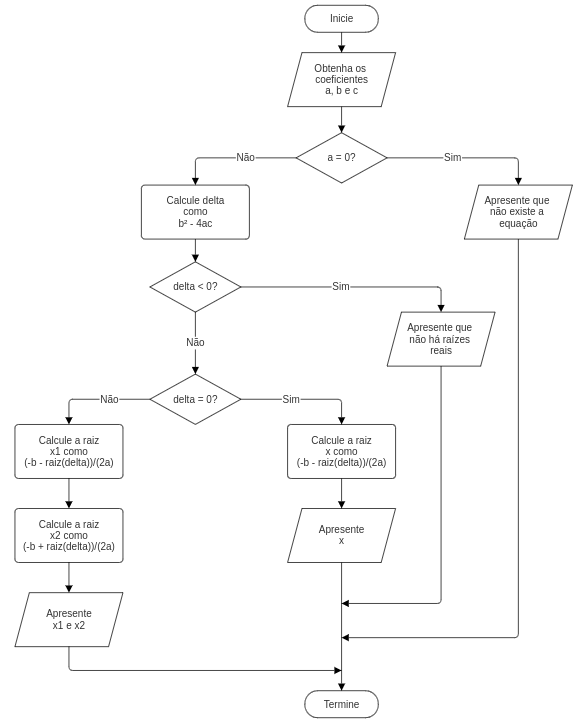
\includegraphics[width=0.6\linewidth,height=\textheight,keepaspectratio]{figuras/fluxograma-raizes-equacao.png}

}

\end{figure}%

\subsection{Pseudocódigo}\label{pseudocuxf3digo}

Como alternativa aos fluxogramas, é bastante comum o emprego do chamado
pseudocódigo, o qual se assemelha a programas, mas é uma abstração da
solução. O Algoritmo~\ref{alg-pseudocodigo-raizes-equacao} é apresentado
na forma de pseudocódigo.

O Algoritmo~\ref{alg-pseudocodigo-raizes-equacao} se refere à mesma
solução lógica da Figura~\ref{fig-fluxograma-raizes-equacao}.

\begin{algorithm}
\caption{\label{alg-pseudocodigo-raizes-equacao}Pseudocódigo para o
cálculo e apresentação das raízes reais de uma equação de segundo grau.}
\begingroup%

\begin{algorithmic}
    \Description Cálculo e apresentação das raízes reais de uma equação de segundo grau na forma ${ax^2 + bx + c = 0}$
    \Require Os coeficientes $a$, $b$ e $c$ da equação
    \Ensure as raízes reais da equação; ou mensagem que a equação é inválida; ou mensagem que não há raízes reais
    \Statex{}
    \Statep{Obtenha os valores de $a$, $b$ e $c$}[Coeficientes da equação]
    \If{$a$ for igual a zero}
        \Statep{Apresente que a equação não é do segundo grau}
    \Else
        \Statep{Calcule o discriminante $\Delta$ como $b^2 - 4ac$}
        \If{$\Delta$ for negativo}[Não há raízes reais]
            \Statep{Apresente que não há raízes reais}
        \ElsIf{$\Delta$ for igual a zero}[Apenas uma raiz]
            \Statep{Calcule $x$ como $-\dfrac{b}{2a}$}
            \Statep{Apresente o valor de $x$}
        \Else[Duas raízes]
            \Statep{Calcule $x_1$ como $\dfrac{-b - \sqrt{\Delta}}{2a}$}
            \Statep{Calcule $x_2$ como $\dfrac{-b + \sqrt{\Delta}}{2a}$}
            \Statep{Apresente $x_1$ e $x_2$}
        \EndIf
    \EndIf 
\end{algorithmic}

\endgroup
\end{algorithm}

\section{Algoritmos e programas}\label{algoritmos-e-programas}

O Algoritmo~\ref{alg-pseudocodigo-conversao-celsius-fahrenheit} é um
algoritmo computacional simples com uma solução para a conversão de
temperaturas entre duas escalas termométricas: de graus Celsius para
Fahrenheit.

\begin{algorithm}
\caption{\label{alg-pseudocodigo-conversao-celsius-fahrenheit}Conversão
de graus Celsius para Fahrenheit.}
\begingroup%

\begin{algorithmic}
    \Description Conversão de escalas termométricas, de graus Celsius para Fahrenheit
    \Require O valor da temperatura em graus Celsius
    \Ensure O valor da temperatura em Fahrenheit
    \Statex{}
    \Statep{Obtenha \Id{celsius}}
    \Statep{Calcule \Id{fahrenheit} como $\dfrac{5}{9}\Id{celsius} + 32$}
    \Statep{Apresente \Id{fahrenheit}}
\end{algorithmic}

\endgroup
\end{algorithm}

Para exemplificar como esse algoritmo pode se tornar um programa, seguem
exemplos de sua implementação em algumas linguagens distintas, sendo
importante salientar a grande variação de formatos de comandos e da
estrutura de cada linguagem.

Pascal:

\begin{Shaded}
\begin{Highlighting}[]
\CommentTok{(*}
\CommentTok{Conversão de escalas termométricas, de graus Celsius para Fahrenheit}
\CommentTok{Requer: a temperatura em graus Celsius}
\CommentTok{Assegura: a temperatura em Fahrenheit}
\CommentTok{*)}
\KeywordTok{program}\NormalTok{ ConversaoTemperaturas;}
\KeywordTok{var}
\NormalTok{    Celsius, Fahrenheit: }\DataTypeTok{real}\NormalTok{;}
\KeywordTok{begin}
    \KeywordTok{read}\NormalTok{(Celsius);}
\NormalTok{    Fahrenheit := }\DecValTok{9}\NormalTok{ / }\DecValTok{5}\NormalTok{ * Celsius + }\DecValTok{32}\NormalTok{;}
    \KeywordTok{write}\NormalTok{(Fahrenheit:}\DecValTok{5}\NormalTok{:}\DecValTok{2}\NormalTok{);}
\KeywordTok{end}\NormalTok{.}
\end{Highlighting}
\end{Shaded}

Python:

\begin{Shaded}
\begin{Highlighting}[]
\CommentTok{\# Conversão de escalas termométricas, de graus Celsius para Fahrenheit}
\CommentTok{\# Pré{-}condição: a temperatura em graus Celsius}
\CommentTok{\# Pós{-}condição: a temperatura em Fahrenheit}

\NormalTok{celsius }\OperatorTok{=} \BuiltInTok{float}\NormalTok{(}\BuiltInTok{input}\NormalTok{())}
\NormalTok{fahrenheit }\OperatorTok{=} \DecValTok{9} \OperatorTok{/} \DecValTok{5} \OperatorTok{*}\NormalTok{ celsius }\OperatorTok{+} \DecValTok{32}
\BuiltInTok{print}\NormalTok{(}\SpecialStringTok{f"}\SpecialCharTok{\{}\NormalTok{fahrenheit}\SpecialCharTok{:.2f\}}\SpecialStringTok{"}\NormalTok{)}
\end{Highlighting}
\end{Shaded}

C:

\begin{Shaded}
\begin{Highlighting}[]
\CommentTok{/*}
\CommentTok{Conversão de escalas termométricas, de graus Celsius para Fahrenheit}
\CommentTok{Requer: a temperatura em graus Celsius}
\CommentTok{Assegura: a temperatura em Fahrenheit}
\CommentTok{*/}
\PreprocessorTok{\#include }\ImportTok{\textless{}stdio.h\textgreater{}}

\DataTypeTok{int}\NormalTok{ main}\OperatorTok{(}\DataTypeTok{void}\OperatorTok{)} \OperatorTok{\{}
    \DataTypeTok{char}\NormalTok{ entrada}\OperatorTok{[}\DecValTok{160}\OperatorTok{];}

\NormalTok{    fgets}\OperatorTok{(}\NormalTok{entrada}\OperatorTok{,} \KeywordTok{sizeof}\NormalTok{ entrada}\OperatorTok{,}\NormalTok{ stdin}\OperatorTok{);}
    \DataTypeTok{double}\NormalTok{ celsius}\OperatorTok{;}
\NormalTok{    sscanf}\OperatorTok{(}\NormalTok{entrada}\OperatorTok{,} \StringTok{"}\SpecialCharTok{\%ld}\StringTok{"}\OperatorTok{,} \OperatorTok{\&}\NormalTok{celsius}\OperatorTok{);}

    \DataTypeTok{double}\NormalTok{ fahrenheit }\OperatorTok{=} \OperatorTok{(}\DataTypeTok{double}\OperatorTok{)}\DecValTok{9} \OperatorTok{/} \DecValTok{5} \OperatorTok{*}\NormalTok{ celsius }\OperatorTok{+} \DecValTok{32}\OperatorTok{;}
\NormalTok{    printf}\OperatorTok{(}\StringTok{"}\SpecialCharTok{\%.2f}\StringTok{"}\OperatorTok{,}\NormalTok{ fahrenheit}\OperatorTok{);}

    \ControlFlowTok{return} \DecValTok{0}\OperatorTok{;}
\OperatorTok{\}}
\end{Highlighting}
\end{Shaded}

R:

\begin{Shaded}
\begin{Highlighting}[]
\CommentTok{\# Conversão de escalas termométricas, de graus Celsius para Fahrenheit}
\CommentTok{\# Pré{-}condição: a temperatura em graus Celsius}
\CommentTok{\# Pós{-}condição: a temperatura em Fahrenheit}

\NormalTok{celsius }\OtherTok{\textless{}{-}} \FunctionTok{as.numeric}\NormalTok{(}\FunctionTok{readline}\NormalTok{(}\StringTok{""}\NormalTok{))}
\NormalTok{fahrenheit }\OtherTok{\textless{}{-}}\NormalTok{ celsius }\SpecialCharTok{*} \DecValTok{9} \SpecialCharTok{/} \DecValTok{5} \SpecialCharTok{+} \DecValTok{32}
\FunctionTok{cat}\NormalTok{(fahrenheit, }\StringTok{"}\SpecialCharTok{\textbackslash{}n}\StringTok{"}\NormalTok{)}
\end{Highlighting}
\end{Shaded}

Java:

\begin{Shaded}
\begin{Highlighting}[]
\CommentTok{// Conversão de escalas termométricas, de graus Celsius para Fahrenheit}
\CommentTok{// Pré{-}condição: a temperatura em graus Celsius}
\CommentTok{// Pós{-}condição: a temperatura em Fahrenheit}

\KeywordTok{import} \ImportTok{java}\OperatorTok{.}\ImportTok{util}\OperatorTok{.}\ImportTok{Scanner}\OperatorTok{;}

\KeywordTok{public} \KeywordTok{class}\NormalTok{ ConversorTemperatura }\OperatorTok{\{}
    \KeywordTok{public} \DataTypeTok{static} \DataTypeTok{void} \FunctionTok{main}\OperatorTok{(}\BuiltInTok{String}\OperatorTok{[]}\NormalTok{ args}\OperatorTok{)} \OperatorTok{\{}
        \BuiltInTok{Scanner}\NormalTok{ scanner }\OperatorTok{=} \KeywordTok{new} \BuiltInTok{Scanner}\OperatorTok{(}\BuiltInTok{System}\OperatorTok{.}\FunctionTok{in}\OperatorTok{);}
        \DataTypeTok{double}\NormalTok{ celsius }\OperatorTok{=}\NormalTok{ scanner}\OperatorTok{.}\FunctionTok{nextDouble}\OperatorTok{();}

        \DataTypeTok{double}\NormalTok{ fahrenheit }\OperatorTok{=}\NormalTok{ celsius }\OperatorTok{*} \DecValTok{9} \OperatorTok{/} \DecValTok{5} \OperatorTok{+} \DecValTok{32}\OperatorTok{;}
        \BuiltInTok{System}\OperatorTok{.}\FunctionTok{out}\OperatorTok{.}\FunctionTok{println}\OperatorTok{(}\NormalTok{fahrenheit}\OperatorTok{);}
        
\NormalTok{        scanner}\OperatorTok{.}\FunctionTok{close}\OperatorTok{();}
    \OperatorTok{\}}
\OperatorTok{\}}
\end{Highlighting}
\end{Shaded}

Ada:

\begin{Shaded}
\begin{Highlighting}[]
\CommentTok{{-}{-} Conversão de escalas termométricas, de graus Celsius para Fahrenheit}
\CommentTok{{-}{-} Pré{-}condição: a temperatura em graus Celsius}
\CommentTok{{-}{-} Pós{-}condição: a temperatura em Fahrenheit}

\KeywordTok{with}\NormalTok{ Ada}\OperatorTok{.}\NormalTok{Text\_IO; }\KeywordTok{use}\NormalTok{ Ada}\OperatorTok{.}\NormalTok{Text\_IO;}

\KeywordTok{procedure}\NormalTok{ Conversor\_Temperatura }\KeywordTok{is}
\NormalTok{   Celsius }\OperatorTok{:} \DataTypeTok{Float}\NormalTok{;}
\NormalTok{   Fahrenheit }\OperatorTok{:} \DataTypeTok{Float}\NormalTok{;}

\KeywordTok{begin}
\NormalTok{   Get}\OperatorTok{(}\NormalTok{Item }\OperatorTok{=\textgreater{}}\NormalTok{ Celsius}\OperatorTok{)}\NormalTok{;}
\NormalTok{   Fahrenheit }\OperatorTok{:=}\NormalTok{ Celsius }\OperatorTok{*} \FloatTok{9.0} \OperatorTok{/} \FloatTok{5.0} \OperatorTok{+} \FloatTok{32.0}\NormalTok{;}
\NormalTok{   Put\_Line}\OperatorTok{(}\NormalTok{Float\textquotesingle{}Image}\OperatorTok{(}\NormalTok{Fahrenheit}\OperatorTok{))}\NormalTok{;}
\KeywordTok{end}\NormalTok{ Conversor\_Temperatura;}
\end{Highlighting}
\end{Shaded}

Lua:

\begin{Shaded}
\begin{Highlighting}[]
\CommentTok{{-}{-} Conversão de escalas termométricas, de graus Celsius para Fahrenheit}
\CommentTok{{-}{-} Pré{-}condição: a temperatura em graus Celsius}
\CommentTok{{-}{-} Pós{-}condição: a temperatura em Fahrenheit}

\KeywordTok{local} \VariableTok{celsius} \OperatorTok{=} \FunctionTok{tonumber}\OperatorTok{(}\FunctionTok{io.read}\OperatorTok{())}
\KeywordTok{local} \VariableTok{fahrenheit} \OperatorTok{=} \VariableTok{celsius} \OperatorTok{*} \DecValTok{9} \OperatorTok{/} \DecValTok{5} \OperatorTok{+} \DecValTok{32}
\FunctionTok{print}\OperatorTok{(}\VariableTok{fahrenheit}\OperatorTok{)}
\end{Highlighting}
\end{Shaded}

Existe, claramente, uma distância entre a solução (algoritmo) e sua
implementação (código da linguagem).

O principal conceito por trás dos algoritmos é ter uma solução mais
abstrata, a qual não se restringe aos detalhes que cada linguagem impõe
e, entretanto, apresenta uma solução simples de entender e objetiva
quanto a como o problema abordado é resolvido.

Este livro não aborda o desenvolvimento de algoritmos, porém faz uso
deles quando necessário, dada a inteção de deixar clara uma solução
antes de apresentar sua implementação em C. Esta estratégia visa
auxiliar o programador menos experiente ou com menor familiaridade com a
linguagem a identificar o que fazem as instruções do programa.

\part{Programação básica}

\chapter{Introdução à linguagem
C}\label{introduuxe7uxe3o-uxe0-linguagem-c}

Neste capítulo é feita a apresentação da linguagem C, um pouco de suas
origens e a evolução de sua especificação. Juntamente a essa introdução,
a compilação e os conceitos de código fonte, objeto e executável também
são tratados.

\section{Origens da linguagem C}\label{origens-da-linguagem-c}

Conhecer um pouco do caminho de uma das mais importantes linguagens de
programação deve trazer ao programador, de certa forma, uma sensação de
pertencimento e autoridade no uso dessa linguagem.

A inspiração da linguagem C veio das linguagens BCPL e B, ambas
projetadas para a implementação de sistemas operacionais. Muitos
elementos de C se originaram dessas linguagens.

C surgiu como uma linguagem de propósito geral que incorporava os
principais mecanismos de controle de fluxo, como condicionais e
estruturas de repetição, juntamente com estruturas de dados como
arranjos e registros. A linguagem não foi estruturada como tendo um alto
nível de abstração e não foca em nenhuma área de aplicação em
particular.

Dennis Ritchie projetou e implementou a linguagem C em um DEC~PDP-11, o
qual usava o sistema operacional UNIX. Na realidade, tanto o compilador
C quanto o próprio sistema operacional foram implementados em C. Esse
desenvolvimento ocorreu de 1969 a 1973. Também à época, compiladores C
já haviam sido implementados para executar em diversas outras máquinas,
como equipamentos IBM, Honeywell e Interdata.

Este histórico foi baseado em \textcite{richards1969},
\textcite{johnson1973}, \textcite{ritchie1978} e \textcite{ritchie1993}.

Segundo consulta ao índice de popularidade elaborado pela
TIOBE\footnote{TIOBE: \url{http://www.tiobe.com}.}, C permanece como uma
das linguagens de programação mais populares mundialmente, disputando os
primeiros lugares com Python, C++ e Java (dados de novembro de 2023).

\subsection{Padronização da
linguagem}\label{sec-padronizacao-da-linguagem}

Sem uma padronização \emph{de facto} da linguagem C nos anos seguintes a
sua criação, havia uma liberdade grande demais na implementação dos
diversos compiladores que apareceram. A especificação conhecida por
K\&R~C era, na ocasião, a única disponível.

De 1983 a 1989, o American National Standards Institute (ANSI) formou um
grupo de trabalho para a padronização da linguagem, estabelecendo, ao
final o padrão conhecido por C89 ou ANSI~C. Esse mesmo padrão foi
reeditado em 1990, com o rótulo C90, porém sem modificações relevantes
na especificação.

Uma extensão foi incorporada à especificação em 1995, com novas
definições e adições à biblioteca padrão. Este padrão foi chamado de
C95.

Modificações significativas na linguagem foram introduzidas no padrão
C99, finalizado em 1999 e adotado a partir do ano 2000. Merecem destaque
novos tipos de dados, como \texttt{long\ long} e \texttt{\_Bool}, a
incorporação de arranjos de comprimento definido durante a execução, a
inclusão de novos cabeçalhos de bibliotecas, a possibilidade de
comentários com \texttt{//}, a mistura de declarações e código e funções
\emph{inline}.

Em 2011 foi publicada a especificação C11, a qual provê suporte a
caracteres Unicode, expressões com tipos genéricos (\texttt{\_Generic})
e execução paralela multi-plataforma com \texttt{threads.h}.

O padrão atual para a linguagem C, no momento da escrita deste texto, é
o C17, publicado em 2018. O C17 não acrescenta novos recursos à
linguagem, porém corrige falhas na versão C11. A especificação C17
também é referenciada como C18.

Neste ano de 2023 é esperada a próxima edição do padrão da linguagem~C,
informalmente designado C23.

A especificação K\&R~C foi descrita em \textcite{ritchie1978}; as demais
especificações estão apropriadamente descritas em
\textcite{cprogramminglanguage}.

\section{Programa básico}\label{programa-buxe1sico}

Programar em C não é tão complexo, mas também não é tão natural. Muitos
aspectos básicos da linguagem requereriam, em teoria, um conhecimento
mais sólido sobre o que são variáveis, como estas existem na memória e
como podem ser manipuladas.

Em um primeiro momento, estes detalhes serão ignorados, visto que é
possível começar a programar e apenas aceitar que algumas coisas são
assim mesmo. Para estes detalhes, por enquanto, basta pensar ``não sei,
só sei que foi assim''\footnote{Como diria Chicó, em \emph{Auto da
  Compadecida}, peça de teatro de Ariano Suassuna também retratada em
  uma minissérie de televisão.}.

\subsection{Primeiro programa: um programa mínimo (e
inútil)}\label{sec-programa-minimo}

Para começar diferente, o primeiro programa exemplo não será o
\emph{Hello, world!}, amplamente utilizado na literatura e em tutoriais.
Ele será o código mínimo na linguagem que é válido e coerente. Por ser
mínimo, porém, não faz nada útil.

\begin{Shaded}
\begin{Highlighting}[]
\DataTypeTok{int}\NormalTok{ main}\OperatorTok{(}\DataTypeTok{void}\OperatorTok{)} \OperatorTok{\{}
    \ControlFlowTok{return} \DecValTok{0}\OperatorTok{;}
\OperatorTok{\}}
\end{Highlighting}
\end{Shaded}

Mesmo sendo minimalista, este código contém vários elementos
interessantes:

\begin{itemize}
\tightlist
\item
  A função \texttt{main} e seu bloco de comandos
\item
  O comando \texttt{return}
\end{itemize}

Um bloco de comandos é uma coleção de comandos delimitados por chaves. O
nome \texttt{main} é associado a esse bloco de comandos, que contém
apenas um comando simples (o \texttt{return\ 0;}) neste caso. Os tipos
\texttt{int} e \texttt{void} indicados não são relevantes neste momento.
Chamar o bloco de comandos de \emph{main} (principal) é obrigatório,
pois indica onde a execução do programa começa.

Neste exemplo, há um único comando dentro de \texttt{main}:
\texttt{return\ 0;}. Este comando indica que, ao ser terminado, o
programa devolve ao sistema operacional um valor inteiro, que é um
indicador que indica em que condições o programa encerrou sua execução.
Por convenção, o valor zero significa que a execução se encerrou sem
erros.

Ao ser compilado e executado, este programa apenas indica ao sistema
operacional que terminou sem erros.

\subsection{\texorpdfstring{Segundo programa: \emph{Hello,
world!}}{Segundo programa: Hello, world!}}\label{segundo-programa-hello-world}

O segundo exemplo expande o código anterior, agora para apresentar uma
mensagem na tela. Para isso, ele usa uma função chamada \texttt{printf},
responsável por apresentar uma saída formatada.

\begin{Shaded}
\begin{Highlighting}[]
\PreprocessorTok{\#include }\ImportTok{\textless{}stdio.h\textgreater{}}

\DataTypeTok{int}\NormalTok{ main}\OperatorTok{(}\DataTypeTok{void}\OperatorTok{)} \OperatorTok{\{}
\NormalTok{    printf}\OperatorTok{(}\StringTok{"Hello, world!}\SpecialCharTok{\textbackslash{}n}\StringTok{"}\OperatorTok{);}
    \ControlFlowTok{return} \DecValTok{0}\OperatorTok{;}
\OperatorTok{\}}
\end{Highlighting}
\end{Shaded}

\begin{Shaded}
\begin{Highlighting}[]
\NormalTok{Hello, world!}
\end{Highlighting}
\end{Shaded}

Este programa, além do \texttt{printf}, também usa a linha
\texttt{\#include\ \textless{}stdio.h\textgreater{}}. O arquivo
\texttt{stdio.h} é um arquivo de cabeçalho (\texttt{stdio} significa
\emph{standard input and output} e \texttt{.h} indica \emph{header}) e
contém informações sobre como o \texttt{printf} deve ser processado pelo
compilador. Este arquivo de cabeçalho descreve uma série de funções para
entradas e saídas feitas pelos programas.

O argumento do \texttt{printf} é o texto \emph{Hello, world!}. Em C,
textos são sempre especificados entre aspas duplas. No exemplo,
\texttt{\textbackslash{}n} é um indicador para mudar para a linha
seguinte.

Um outro detalhe no código ainda pode ser destacado: cada comando
simples é terminado com um ponto e vírgula, que é o caso tanto do
\texttt{printf} quanto do \texttt{return}.

Na sequência é apresentada a versão definitiva do código do \emph{Hello,
world!}.

\begin{Shaded}
\begin{Highlighting}[]
\CommentTok{/*}
\CommentTok{Programa "Hello, world": código exemplo do clássico primeiro programa em C}
\CommentTok{    que apenas apresenta uma mensagem de saudação na tela}
\CommentTok{Assegura: a apresentação da mensagem padrão "Hello, world"}
\CommentTok{*/}
\PreprocessorTok{\#include }\ImportTok{\textless{}stdio.h\textgreater{}}

\DataTypeTok{int}\NormalTok{ main}\OperatorTok{(}\DataTypeTok{void}\OperatorTok{)} \OperatorTok{\{}
\NormalTok{    printf}\OperatorTok{(}\StringTok{"Hello, world!}\SpecialCharTok{\textbackslash{}n}\StringTok{"}\OperatorTok{);}
    \ControlFlowTok{return} \DecValTok{0}\OperatorTok{;}
\OperatorTok{\}}
\end{Highlighting}
\end{Shaded}

\begin{Shaded}
\begin{Highlighting}[]
\NormalTok{Hello, world!}
\end{Highlighting}
\end{Shaded}

Esta versão acrescenta a documentação do código. Qualquer texto colocado
entre \texttt{/*} e \texttt{*/} é um comentário e é ignorado
completamente pelo compilador ao analisar o código fonte. Os comentários
não são para o compilador, mas para humanos que lerão o código do
programa.

Neste caso específico, o comentário tem a função de documentar o
propósito do código. Ele fornece uma descrição do propósito do código e
dá informações relevantes. O grau de detalhe depende sempre do contexto;
códigos simples podem ter documentação mais simples, enquanto programas
que fazem parte de um projeto compartilhado entre vários desenvolvedores
deve conter as informações necessárias para que todos da equipe os
compreendam.

\section{Comandos simples}\label{comandos-simples}

\index{comando!simples} Um componente estrutural da linguagem é o
chamado comando simples. Esse comando de caracteriza por uma instrução
individual no código do programa.

Os comandos simples seguem uma sintaxe também simples.

\begin{tcolorbox}[enhanced jigsaw, colback=white, arc=.35mm, colframe=quarto-callout-color-frame, toprule=.15mm, leftrule=.75mm, left=2mm, rightrule=.15mm, bottomrule=.15mm, opacityback=0, breakable]

\vspace{-3mm}\textbf{Comando simples}\vspace{3mm}

\emph{instrução} ;

\end{tcolorbox}

Nos exemplos dados, cada \texttt{printf} usado para apresentar uma
informação e também o \texttt{return\ 0} são comandos simples e, desta
forma, obrigatoriamente terminados com um ponto e vírgula. A execução do
\texttt{printf} é uma \emph{instrução}, assim como o término da execução
indicado pelo \texttt{return}.

Segue um exemplo simples de programa com alguns comandos simples.

\begin{Shaded}
\begin{Highlighting}[]
\CommentTok{/*}
\CommentTok{Apresentação de uma série de mensagens na tela}
\CommentTok{*/}
\PreprocessorTok{\#include }\ImportTok{\textless{}stdio.h\textgreater{}}

\DataTypeTok{int}\NormalTok{ main}\OperatorTok{(}\DataTypeTok{void}\OperatorTok{)} \OperatorTok{\{}
\NormalTok{    printf}\OperatorTok{(}\StringTok{"Bom dia! "}\OperatorTok{);}
\NormalTok{    printf}\OperatorTok{(}\StringTok{"Este é um exemplo de "}\OperatorTok{);}
\NormalTok{    printf}\OperatorTok{(}\StringTok{"vários comandos simples.}\SpecialCharTok{\textbackslash{}n}\StringTok{"}\OperatorTok{);}
\NormalTok{    printf}\OperatorTok{(}\StringTok{"Todos são execuções do printf e todos são finalizados com \textquotesingle{};\textquotesingle{}.}\SpecialCharTok{\textbackslash{}n}\StringTok{"}\OperatorTok{);}
\NormalTok{    printf}\OperatorTok{(}\StringTok{"O \textquotesingle{}return 0\textquotesingle{}, naturalmente, também é um comando simples.}\SpecialCharTok{\textbackslash{}n}\StringTok{"}\OperatorTok{);}

    \ControlFlowTok{return} \DecValTok{0}\OperatorTok{;}
\OperatorTok{\}}
\end{Highlighting}
\end{Shaded}

\begin{Shaded}
\begin{Highlighting}[]
\NormalTok{Bom dia! Este é um exemplo de vários comandos simples.}
\NormalTok{Todos são execuções do printf e todos são finalizados com \textquotesingle{};\textquotesingle{}.}
\NormalTok{O \textquotesingle{}return 0\textquotesingle{}, naturalmente, também é um comando simples.}
\end{Highlighting}
\end{Shaded}

\begin{tcolorbox}[enhanced jigsaw, arc=.35mm, bottomtitle=1mm, colbacktitle=quarto-callout-tip-color!10!white, title=\textcolor{quarto-callout-tip-color}{\faLightbulb}\hspace{0.5em}{Dica}, toprule=.15mm, left=2mm, opacityback=0, colback=white, colframe=quarto-callout-tip-color-frame, opacitybacktitle=0.6, bottomrule=.15mm, leftrule=.75mm, toptitle=1mm, coltitle=black, titlerule=0mm, rightrule=.15mm, breakable]

Embora a linguagem C não tenha objeções quando a escrever dois comandos
simples em uma única linha do programa, sugere-se forntemente que cada
comando tenha sua própria linha.

\end{tcolorbox}

\begin{tcolorbox}[enhanced jigsaw, arc=.35mm, bottomtitle=1mm, colbacktitle=quarto-callout-warning-color!10!white, title={Curiosidade}, toprule=.15mm, left=2mm, opacityback=0, colback=white, colframe=quarto-callout-warning-color-frame, opacitybacktitle=0.6, bottomrule=.15mm, leftrule=.75mm, toptitle=1mm, coltitle=black, titlerule=0mm, rightrule=.15mm, breakable]

Em C, existe a possibilidade de que o comando simples seja vazio. Para
especificá-lo, bastar inserir o ponto e vírgula.

\begin{Shaded}
\begin{Highlighting}[]
\NormalTok{    printf}\OperatorTok{(}\StringTok{"Um!"}\OperatorTok{);}
    \OperatorTok{;}  \CommentTok{// comando vazio que não faz nada...}
\NormalTok{    printf}\OperatorTok{(}\StringTok{"Dois!"}\OperatorTok{);}
\end{Highlighting}
\end{Shaded}

Resta pensar quando um comando que não faz nada pode ser útil.

\end{tcolorbox}

\section{Código fonte, objeto e
executável}\label{cuxf3digo-fonte-objeto-e-executuxe1vel}

Todos os programas em C são escritos em arquivos de texto simples, que
são os que não dão suporte a negrito e itálico, tipos de fonte ou
formatação de parágrafo, entre outros recursos. O código em C segue uma
sintaxe bastante específica e os programas escritos são chamados de
código fonte.

Para um programa escrito em C ser executado, primeiramente é necessário
que ele seja compilado. O compilador é um programa cuja atribuição
principal é analisar o código fonte, interpretando as letras, símbolos e
dígitos ali escritos e gerar o código objeto, que é o código compilado.
O código objeto é guardado em um arquivo e já não é mais legível por
humanos, já que contém as instruções que o processador é capaz de
entender e executar.

O código fonte, depois de compilado, leva a um código objeto que é
dependente da máquina. Assim, são produzidos códigos objeto específicos
para processadores x86, ARM ou outro. Para que um mesmo programa possa
ser executado em plataformas diferentes, é preciso que ele seja
compilado para cada plataforma alvo individualmente.

Há inúmeros compiladores disponíveis para C, como o GNU e o CLang, por
exemplo. Também há implementações de compiladores específicos para cada
plataforma de sistema operacional e e de processador. Ou seja, há um
compilador GNU para Windows executando em processadores x86 e outro para
Linux em um processador ARM. Cada compilador um possui suas próprias
regras internas, mas todos obedecem especificações rigorosas e
padronizadas. Desta forma, independente do hardware e do sistema
operacional, um mesmo código fonte, ao ser compilado e executado, produz
um mesmo resultado. Isso é uma regra e, para ela, naturalmente há
exceções.

Neste texto, a especificação conhecida como C17 (da ISO) é a adotada
para todas as implementações. Os programas são compilador usando o
compilador GNU em um sistema operacional Linux, tudo sobre um hardware
x86.

Finalmente, ainda há uma última etapa, na qual o código compilado é
colocado em um arquivo que o sistema operacional da vez consegue
carregar para a memória e colocá-lo em execução. Este é chamado de
código executável e também depende da plataforma.

Usualmente a etapa do código objeto é escondida de quem usa o compilador
e, aparentemente, do código fonte é gerado diretamente o executável. Na
prática, esse é o efeito final.

\subsection{\texorpdfstring{Compilação com o
\texttt{gcc}}{Compilação com o gcc}}\label{compilauxe7uxe3o-com-o-gcc}

Há uma diversidade de compiladores para a linguagem C, além de diversos
IDEs\footnote{Um ambiente de desenvolvimento integrado, ou
  \emph{integrated development environment} (IDE), é um programa que dá
  suporte para escrever programas, provendo um editor de texto dedicado,
  destaque de sintaxe (diferentes elementos do programa aparecem em
  cores diferenciadas), acesso ao compilador com o clique de um botão ou
  uma combinação simples no teclado.} com diferentes facilidades para
escrever códigos fonte. Há IDEs que podem ser instalados, como Visual
Studio Code\footnote{Visual Studio Code:
  \url{https://code.visualstudio.com}.}, Code::Blocks\footnote{Code::Blocks:
  \url{https://www.codeblocks.org}.}, Visual Studio\footnote{Visual
  Studio: \url{https://visualstudio.microsoft.com}.} ou
Eclipse\footnote{Eclipse: \url{https://www.eclipse.org}.}, por exemplo,
além das disponíveis \emph{online}, como GDB\footnote{GDB Online:
  \url{https://www.onlinegdb.com}.}, Programiz\footnote{Programiz:
  \url{https://www.programiz.com}.} ou Replit\footnote{Replit:
  \url{https://replit.com}.}.

Neste livro os programas foram compilados invocando no terminal o
compilador GNU GCC\footnote{Gnu Compiler Collection:
  \url{https://gcc.gnu.org}.} na versão mais recente disponível no
repositório oficial do Debian.

\begin{Shaded}
\begin{Highlighting}[]
\NormalTok{$ }\KeywordTok{gcc {-}{-}version}
\NormalTok{gcc (Ubuntu 13.3.0{-}6ubuntu2\textasciitilde{}24.04) 13.3.0}
\NormalTok{Copyright (C) 2023 Free Software Foundation, Inc.}
\NormalTok{This is free software; see the source for copying conditions.  There is NO}
\NormalTok{warranty; not even for MERCHANTABILITY or FITNESS FOR A PARTICULAR PURPOSE.}

\end{Highlighting}
\end{Shaded}

As opções \texttt{-Wall} e \texttt{-pedantic} são incluídas
automaticamente e ativam uma vasta gama de mensagens de erro e avisos
importantes, dando maior controle sobre o código executável que está
sendo gerado. A especificação C17 da linguagem C é adotada com a opção
\texttt{-std=c17} (Seção~\ref{sec-padronizacao-da-linguagem}).

\begin{Shaded}
\begin{Highlighting}[]
\BuiltInTok{alias}\NormalTok{ gcc=}\StringTok{\textquotesingle{}gcc {-}Wall {-}pedantic {-}std=c17\textquotesingle{}}
\end{Highlighting}
\end{Shaded}

Para exemplificar, considere um arquivo com nome \texttt{bom\_dia.c} com
código fonte seguinte.

\begin{Shaded}
\begin{Highlighting}[]
\CommentTok{/*}
\CommentTok{Apresentação um bom dia!}
\CommentTok{Assegura: uma mensagem de bom dia apresentada na tela}
\CommentTok{*/}
\PreprocessorTok{\#include }\ImportTok{\textless{}stdio.h\textgreater{}}

\DataTypeTok{int}\NormalTok{ main}\OperatorTok{(}\DataTypeTok{void}\OperatorTok{)} \OperatorTok{\{}
\NormalTok{    printf}\OperatorTok{(}\StringTok{"Bom dia! Que seu dia seja ótimo!}\SpecialCharTok{\textbackslash{}n}\StringTok{"}\OperatorTok{);}

    \ControlFlowTok{return} \DecValTok{0}\OperatorTok{;}
\OperatorTok{\}}
\end{Highlighting}
\end{Shaded}

Usando o comando \texttt{file} é possível ver (ou tentar ver) o tipo de
informação guardada em um arquivo. Para o caso do código fonte, o
arquivo é identificado como \emph{C source code}, ou seja, código fonte
em C.

\begin{Shaded}
\begin{Highlighting}[]
\NormalTok{$ }\KeywordTok{file bom\_dia.c}
\NormalTok{bom\_dia.c: C source, Unicode text, UTF{-}8 text}
\end{Highlighting}
\end{Shaded}

A compilação pode ser feita com o comando apresentado. A opção
\texttt{-o} permite nomear o arquivo executável que é criado.

\begin{Shaded}
\begin{Highlighting}[]
\NormalTok{$ }\KeywordTok{gcc {-}Wall {-}pedantic {-}std=c17 bom\_dia.c {-}o bom\_dia}
\end{Highlighting}
\end{Shaded}

Esse comando compila \texttt{bom\_dia.c} e gera o arquivo executável
\texttt{bom\_dia}. No caso de sucesso na compilação, o \texttt{gcc} não
apresenta saídas; apenas eventuais problemas são apresentados na tela.

\begin{Shaded}
\begin{Highlighting}[]
\NormalTok{$ }\KeywordTok{file bom\_dia}
\NormalTok{bom\_dia: ELF 64{-}bit LSB pie executable, x86{-}64, version 1 (SYSV), dynamically }
\NormalTok{linked, interpreter /lib64/ld{-}linux{-}x86{-}64.so.2, }
\NormalTok{BuildID[sha1]=87d67e99709397eb27df650972aaab8300baf796, for GNU/Linux 3.2.0, }
\NormalTok{not stripped}
\end{Highlighting}
\end{Shaded}

A execução de \texttt{file}, nesse caso, apresenta muita informação. A
relevante, neste momento, é que o arquivo contém um \emph{ELF 64-bit LSB
pie executable}, o que quer dizer que é um programa executável.

Na sequência é apresentada a execução do programa \texttt{bom\_dia}.

\begin{Shaded}
\begin{Highlighting}[]
\NormalTok{$ }\KeywordTok{./bom\_dia}
\NormalTok{Bom dia! Que seu dia seja ótimo!}
\end{Highlighting}
\end{Shaded}

\subsection{Erros de sintaxe}\label{erros-de-sintaxe}

Sendo uma linguagem de programação, os comandos são sempre analisados de
forma rígida. A falta de um parêntese, um espaço no lugar errado ou uma
grafia errada (como \texttt{prinft}, por exemplo) já dá margem para o
compilador reclamar que algo está errado e se recusar a gerar o
executável. Esses são os erros de sintaxe e é função do compilador
encontrá-los.

O programador deve aprender a ler as mensagens de erro produzidas pelo
compilador e interpretá-las, permitindo a remoção dos erros sintáticos.

Como exemplo, segue uma versão incorreta do programa exemplo. Nela,
``acidentalmente'' o ponto e vírgula foi esquecido.

\begin{Shaded}
\begin{Highlighting}[]
\CommentTok{/*}
\CommentTok{Programa "Hello, world": código exemplo do clássico primeiro programa em C}
\CommentTok{    que apenas apresenta uma mensagem de saudação na tela}
\CommentTok{Assegura: a apresentação da mensagem padrão "Hello, world"}
\CommentTok{*/}
\PreprocessorTok{\#include }\ImportTok{\textless{}stdio.h\textgreater{}}

\DataTypeTok{int}\NormalTok{ main}\OperatorTok{(}\DataTypeTok{void}\OperatorTok{)} \OperatorTok{\{}
\NormalTok{    printf}\OperatorTok{(}\StringTok{"Hello, world!}\SpecialCharTok{\textbackslash{}n}\StringTok{"}\OperatorTok{)}
    \ControlFlowTok{return} \DecValTok{0}\OperatorTok{;}
\OperatorTok{\}}
\end{Highlighting}
\end{Shaded}

\begin{Shaded}
\begin{Highlighting}[]
\NormalTok{main.c: In function ‘main’:}
\NormalTok{main.c:9:30: error: expected ‘;’ before ‘return’}
\NormalTok{    9 |     printf("Hello, world!\textbackslash{}n")}
\NormalTok{      |                              \^{}}
\NormalTok{      |                              ;}
\NormalTok{   10 |     return 0;}
\NormalTok{      |     \textasciitilde{}\textasciitilde{}\textasciitilde{}\textasciitilde{}\textasciitilde{}\textasciitilde{}                    }
\end{Highlighting}
\end{Shaded}

A mensagem de erro aponta em que linha e coluna deveria haver um ponto e
vírgula.

Os erros são apresentados conforme o compilador consegue detectar,
apresentando mensagens tão boas quanto possível. Além disso, uma única
falha pode desencadear uma sequência de erros, como no exemplo seguinte,
na qual apenas faltou fechar as aspas no argumento da função
\texttt{printf}.

\begin{Shaded}
\begin{Highlighting}[]
\CommentTok{/*}
\CommentTok{Programa "Hello, world": código exemplo do clássico primeiro programa em C}
\CommentTok{    que apenas apresenta uma mensagem de saudação na tela}
\CommentTok{Assegura: a apresentação da mensagem padrão "Hello, world"}
\CommentTok{*/}
\PreprocessorTok{\#include }\ImportTok{\textless{}stdio.h\textgreater{}}

\DataTypeTok{int}\NormalTok{ main}\OperatorTok{(}\DataTypeTok{void}\OperatorTok{)} \OperatorTok{\{}
\NormalTok{    printf}\OperatorTok{(}\StringTok{"Hello, world!}\SpecialCharTok{\textbackslash{}n}\StringTok{);}
    \ControlFlowTok{return} \DecValTok{0}\OperatorTok{;}
\OperatorTok{\}}
\end{Highlighting}
\end{Shaded}

\begin{Shaded}
\begin{Highlighting}[]
\NormalTok{main.c: In function ‘main’:}
\NormalTok{main.c:9:12: warning: missing terminating " character}
\NormalTok{    9 |     printf("Hello, world!\textbackslash{}n);}
\NormalTok{      |            \^{}}
\NormalTok{main.c:9:12: error: missing terminating " character}
\NormalTok{    9 |     printf("Hello, world!\textbackslash{}n);}
\NormalTok{      |            \^{}\textasciitilde{}\textasciitilde{}\textasciitilde{}\textasciitilde{}\textasciitilde{}\textasciitilde{}\textasciitilde{}\textasciitilde{}\textasciitilde{}\textasciitilde{}\textasciitilde{}\textasciitilde{}\textasciitilde{}\textasciitilde{}\textasciitilde{}\textasciitilde{}\textasciitilde{}}
\NormalTok{main.c:10:5: error: expected expression before ‘return’}
\NormalTok{   10 |     return 0;}
\NormalTok{      |     \^{}\textasciitilde{}\textasciitilde{}\textasciitilde{}\textasciitilde{}\textasciitilde{}}
\NormalTok{main.c:10:14: error: expected ‘;’ before ‘\}’ token}
\NormalTok{   10 |     return 0;}
\NormalTok{      |              \^{}}
\NormalTok{      |              ;}
\NormalTok{   11 | \}}
\NormalTok{      | \textasciitilde{}             }
\end{Highlighting}
\end{Shaded}

\subsection{Erros de lógica}\label{erros-de-luxf3gica}

Um programa pode ser compilado e gerar o executável sem erros ou
qualquer tipo de aviso que o compilador esteja ajustado para dar. Mas
apesar disso, a execução não produz o resultado desejado. Neste caso,
mesmo com a sintaxe correta, as instruções contém um erro (uma falha de
cálculo, uma comparação equivocada) que invalida o programa. Esse são os
erros de lógica e, desta vez, cabe ao programador encontrá-los e
corrigi-los.

A evitação de erros de lógica é considerada ao longo de todo o livro.

\chapter{Tipos de dados da linguagem C}\label{sec-tipos-de-dados}

Qualquer linguagem de programação, dentre as milhares existentes, têm
como premissa a manipulação e a transformação de dados. Esta parte do
texto trata de como dados são representados em computação e faz uma
apresentação dos principais tipos de dados usados na linguagem~C.

A ilustração dos tipos de dados, suas limitações e principais
características envolvem, adicionamente, a apresentação da função
\texttt{printf}, responsável por apresentar os dados do programa para o
usuário.

\section{Representação de dados}\label{sec-representacao-de-dados}

Em computação, as informações são estruturadas em bits. A forma mais
básica de circuitos eletrônicos representarem algo é pela ausência ou
presença de corrente elétrica. Assim, um bit é uma parte do circuito que
indica ``desligado'' ou ``ligado'', ``sem corrente elétrica'' ou ``com
corrente elétrica'', ``ausente'' ou ``presente'' ou, simplificadamente,
``zero'' ou ``um''. O uso dos valores binários 0 e 1 é a forma
tradicional de se representar um bit.

Para serem usados de forma prática, os bits são sempre organizados em
sequências de comprimento oito. O grupo de oito bits é chamado de byte.
Nos sistemas computacionais, os circuitos responsáveis por armazenar os
bytes são chamados de memória. Esta é usualmente medida em gigabytes,
sendo cada gigabyte correspondente a 1.073.741.824~bytes
(2\textsuperscript{30}).

Cada byte, com seus oito bits, pode assumir os valores 00000000,
00000001, 00000010, 000000011\ldots{} até 11111111. São
2\textsuperscript{8} possíveis combinações.

Programas manipulam dados, como nomes de localidades, taxas de câmbio,
velocidade de veículos, listas de espera e tantos outros. Para
representar os dados, programas usam essa memória estruturada em bytes.
Tanto as instruções que serão executadas pelo processador quanto os
dados precisam ser representados com bytes.

Para representar um dado qualquer, portanto, é preciso fazer seu
mapeamento para bytes.

A letra \texttt{A} é usualmente representada pelo byte 01000001 e o
símbolo \texttt{!}, pelo 00100001. Essas escolhas foram arbitrárias e o
mapeamento do conjunto básico de caracteres pode ser consultado em uma
tabela chamada de \emph{American Standard Code for Information
Interchange}, ou tabela ASCII\footnote{Existem outras estratégias para
  representação de caracteres, principalmente para incorporar
  acentuações (como \texttt{ñ} do espanhol), caracteres particulares
  (\texttt{ß} do alemão) ou ainda caracteres como os japoneses e
  hebraicos.}. Textos são representados por sequências de bytes
representando os caracteres.

Números inteiros são frequentemente representados por uma certa
quantidade fixa de bytes consecutivos. Assim, considerando-se quatro
bytes para um inteiro, é possível associar a sequência 00000000 00000000
00000000 00000000 ao valor zero, 00000000 00000000 00000000 00000001 ao
valor 1 e assim, sucessivamente, até 11111111 11111111 11111111
11111111, que equivaleria a 4.294.967.295 (ou 2\textsuperscript{32}-1).
Números negativos separam o primeiro bit para indicar o sinal (0~é
positivo, 1~é negativo) e os demais 31~bits seriam usados para
representar os diversos valores, indo de -2.147.483.648 a 2.147.483.647
considerando-se os quatro bytes. Naturalmente, quanto mais bytes, maior
o intervalo de valores representados.

Outros tipos de valores, como números reais, valores lógicos e endereços
internos da memória também escolhem uma estratégia para representar seus
valores usando um mapeamento adequado para um ou mais bytes.

\section{Constantes e seus tipos}\label{sec-constantes-e-seus-tipos}

Tendo em vista que quaisquer dados (números, textos ou qualquer outro)
usam bytes para serem representados, a linguagem C também designa uma
codificação específica para os valores ao interpretar um código fonte.

Nos programas em C, valores explícitos no código, como um texto ou um
valor numérico, é chamado de valor constante. O texto clássico expresso
por \texttt{"Hello,\ world!"} é uma constante literal (textual). Em C,
as constantes com sequências de caracteres são sempre expressas
usando-se aspas duplas.

O código seguinte visa apresentar como saída o valor de \(\pi\), que foi
(grosseiramente) aproximando no código fonte para 3,1416.

\begin{Shaded}
\begin{Highlighting}[]
\CommentTok{/*}
\CommentTok{Apresentação do valor aproximado de pi}
\CommentTok{*/}
\PreprocessorTok{\#include }\ImportTok{\textless{}stdio.h\textgreater{}}

\DataTypeTok{int}\NormalTok{ main}\OperatorTok{(}\DataTypeTok{void}\OperatorTok{)} \OperatorTok{\{}
\NormalTok{    printf}\OperatorTok{(}\StringTok{"pi vale, aproximadamente, }\SpecialCharTok{\%g\textbackslash{}n}\StringTok{"}\OperatorTok{,} \FloatTok{3.1416}\OperatorTok{);}
    \ControlFlowTok{return} \DecValTok{0}\OperatorTok{;}
\OperatorTok{\}}
\end{Highlighting}
\end{Shaded}

\begin{Shaded}
\begin{Highlighting}[]
\NormalTok{pi vale, aproximadamente, 3.1416}
\end{Highlighting}
\end{Shaded}

O comando \texttt{printf} possui dois parâmetros. O primeiro é uma
constante textual com o que deve ser apresentado (elemento obrigatório
da função); o segundo é um valor real expresso na forma de uma constante
(\texttt{3.1416}). O símbolo \texttt{\%g} é um indicador de local usado
para valores reais, ou seja ele representa onde o valor 3,1416 será
inserido no texto.

A constante \texttt{3.1416} (expressa usando o ponto como separador
decimal) possui, em C, o tipo \texttt{double}. Esse tipo corresponde a
uma representação de precisão dupla, seguindo o padrão IEC~60559.
Qualquer constante real em C é representada por um \texttt{double},
exceto quando explicitamente indicado de outra forma.

Constantes inteiras expressas em base 10 são representadas pelo tipo
\texttt{int}, que tem mínimo de 16~bits, embora implementações atuais
comumente usem 32~bits. Com o mínimo de bits, os valores representados
vão de -32.768 a 32.767; já com 32~bits a variação é de -2.147.483.648 a
2.147.483.647. Desta forma, dependendo da implementação do compilador,
os limites podem variar consideravelmente. As constantes inteiras seguem
essa regra, exceto quando declaradas explicitamente com um tipo
específico.

Caso uma constante inteira exceda a capacidade de representação de um
\texttt{int}, um \texttt{long\ int} é usado em seu lugar, partindo de um
mínimo de 32~bits. Essa escolha é transparente para o programador.

\begin{Shaded}
\begin{Highlighting}[]
\CommentTok{/*}
\CommentTok{Apresentação do valor de 5234 elevado ao cubo}
\CommentTok{*/}
\PreprocessorTok{\#include }\ImportTok{\textless{}stdio.h\textgreater{}}

\DataTypeTok{int}\NormalTok{ main}\OperatorTok{(}\DataTypeTok{void}\OperatorTok{)} \OperatorTok{\{}
\NormalTok{    printf}\OperatorTok{(}\StringTok{"O cubo de }\SpecialCharTok{\%d}\StringTok{ é igual a }\SpecialCharTok{\%ld\textbackslash{}n}\StringTok{"}\OperatorTok{,} \DecValTok{5234}\OperatorTok{,} \DecValTok{143384152904}\OperatorTok{);}
    \ControlFlowTok{return} \DecValTok{0}\OperatorTok{;}
\OperatorTok{\}}
\end{Highlighting}
\end{Shaded}

\begin{Shaded}
\begin{Highlighting}[]
\NormalTok{O cubo de 5234 é igual a 143384152904}
\end{Highlighting}
\end{Shaded}

Neste programa, o \texttt{printf} usa a especificação \texttt{\%d},
significando um \texttt{int} apresentado na base 10 (decimal). A
especificação \texttt{\%ld} é usada para um \texttt{long\ int} expresso
em decimal. Os valores são substituídos na ordem em que aparecem no
\texttt{printf}.

Particularmente no compilador usado para produzir esse exemplo, o valor
5.234 pode ser representado em um \texttt{int} e escrito com
\texttt{\%d}; já 143.384.152.904 (5.234\textsuperscript{3}) necessitou
de mais bits e foi automaticamente promovido para um \texttt{long\ int},
cuja especificação de formato é \texttt{\%ld}. O compilador poderá
apresentar um aviso caso o valor maior tente ser escrito apenas com
\texttt{\%d}, embora o executável seja gerado e o resultado apresentado
seja incorreto.

Da mesma forma que há especificadores para valores numéricos, há também
para valores textuais.

\begin{Shaded}
\begin{Highlighting}[]
\CommentTok{/*}
\CommentTok{Apresentação de valores textuais}
\CommentTok{*/}
\PreprocessorTok{\#include }\ImportTok{\textless{}stdio.h\textgreater{}}

\DataTypeTok{int}\NormalTok{ main}\OperatorTok{(}\DataTypeTok{void}\OperatorTok{)} \OperatorTok{\{}
\NormalTok{    printf}\OperatorTok{(}\StringTok{"}\SpecialCharTok{\%s}\StringTok{ é primo de }\SpecialCharTok{\%s\textbackslash{}n}\StringTok{"}\OperatorTok{,} \StringTok{"Nereu"}\OperatorTok{,} \StringTok{"Eutália"}\OperatorTok{);}
\NormalTok{    printf}\OperatorTok{(}\StringTok{"}\SpecialCharTok{\%s}\StringTok{ é prima de }\SpecialCharTok{\%s\textbackslash{}n}\StringTok{"}\OperatorTok{,} \StringTok{"Eutália"}\OperatorTok{,} \StringTok{"Nereu"}\OperatorTok{);}
\NormalTok{    printf}\OperatorTok{(}\StringTok{"}\SpecialCharTok{\%s}\StringTok{ começa com a letra }\SpecialCharTok{\%c\textbackslash{}n}\StringTok{"}\OperatorTok{,} \StringTok{"Yolanda"}\OperatorTok{,} \CharTok{\textquotesingle{}Y\textquotesingle{}}\OperatorTok{);}

    \ControlFlowTok{return} \DecValTok{0}\OperatorTok{;}
\OperatorTok{\}}
\end{Highlighting}
\end{Shaded}

\begin{Shaded}
\begin{Highlighting}[]
\NormalTok{Nereu é primo de Eutália}
\NormalTok{Eutália é prima de Nereu}
\NormalTok{Yolanda começa com a letra Y}
\end{Highlighting}
\end{Shaded}

\index{char@\texttt{char}} A indicação \texttt{\%s} é compatível com
textos de comprimento variado, ou seja, cadeias de caracteres. Por outro
lado, C define um tipo específico para um único caractere: o tipo
\texttt{char}. Ele usa oito bits (mínimo), ou seja, um byte, e é
representado por aspas simples:
\texttt{\textquotesingle{}Y\textquotesingle{}}. Para caracteres simples
do tipo \texttt{char}, usa-se a especificação de formato \texttt{\%c}.

A diferença entre \texttt{"Y"} e
\texttt{\textquotesingle{}Y\textquotesingle{}} é abordada em mais
detalhes no Capítulo~\ref{sec-dados-textuais}.

\section{\texorpdfstring{Mais sobre o
\texttt{printf}}{Mais sobre o printf}}\label{mais-sobre-o-printf}

O nome \texttt{printf} vem de \emph{print formatted}, ou seja, apresente
algo de forma formatada. O uso desta função requer o carregamento do
arquivo de cabeçalho \texttt{stdio.h}.

A função apresenta um texto na saída padrão (a tela do terminal) e este
deve ser o primeiro parâmetro. Além de apresentar o texto, a função
também faz conversões de valores, usando os marcadores iniciados com
\texttt{\%}. Por exemplo, \texttt{\%d} é usado para um valor inteiro
decimal, \texttt{\%g} para apresentar um valor real e \texttt{\%s} é
usado para apresentar valores textuais, chamados cadeias de caracteres
ou \emph{strings}. Outro elemento de formatação são os caracteres
especiais como \texttt{\textbackslash{}n}, que indica a mudança de
linha, \texttt{\textbackslash{}t}, que é uma tabulação similar à dos
editores de texto, ou ainda \texttt{\textbackslash{}"}, que indica aspas
duplas.

Cada marcador com o símbolo \texttt{\%} é substituído em ordem. Assim,
se houver várias substituições, cada uma delas é feita sucessivamente.

\begin{Shaded}
\begin{Highlighting}[]
\CommentTok{/*}
\CommentTok{Exemplo de escrita de vários valores}
\CommentTok{*/}
\PreprocessorTok{\#include }\ImportTok{\textless{}stdio.h\textgreater{}}

\DataTypeTok{int}\NormalTok{ main}\OperatorTok{(}\DataTypeTok{void}\OperatorTok{)} \OperatorTok{\{}
\NormalTok{    printf}\OperatorTok{(}\StringTok{"Meu nome é }\SpecialCharTok{\%s}\StringTok{, nasci em }\SpecialCharTok{\%d}\StringTok{ e ganho R$ }\SpecialCharTok{\%g}\StringTok{ de salário.}\SpecialCharTok{\textbackslash{}n}\StringTok{"}\OperatorTok{,}
        \StringTok{"Fulano"}\OperatorTok{,} \DecValTok{2003}\OperatorTok{,} \FloatTok{2512.17}\OperatorTok{);}

    \ControlFlowTok{return} \DecValTok{0}\OperatorTok{;}
\OperatorTok{\}}
\end{Highlighting}
\end{Shaded}

\begin{Shaded}
\begin{Highlighting}[]
\NormalTok{Meu nome é Fulano, nasci em 2003 e ganho R$ 2512.17 de salário.}
\end{Highlighting}
\end{Shaded}

Para valores inteiros, segue um exemplo para a escrita do valor de uma
expressão usando variações de formato. Algumas opções diferentes de
escrita são acrescentadas.

\begin{Shaded}
\begin{Highlighting}[]
\CommentTok{/*}
\CommentTok{Exemplo de escrita de valores inteiros}
\CommentTok{*/}
\PreprocessorTok{\#include }\ImportTok{\textless{}stdio.h\textgreater{}}

\DataTypeTok{int}\NormalTok{ main}\OperatorTok{(}\DataTypeTok{void}\OperatorTok{)} \OperatorTok{\{}
\NormalTok{    printf}\OperatorTok{(}\StringTok{"Um valor inteiro    : }\SpecialCharTok{\%d\textbackslash{}n}\StringTok{"}\OperatorTok{,} \DecValTok{481}\OperatorTok{);}
\NormalTok{    printf}\OperatorTok{(}\StringTok{"Outro valor inteiro : }\SpecialCharTok{\%8d\textbackslash{}n}\StringTok{"}\OperatorTok{,} \DecValTok{481}\OperatorTok{);}
\NormalTok{    printf}\OperatorTok{(}\StringTok{"E mais outro        : }\SpecialCharTok{\%08d\textbackslash{}n}\StringTok{"}\OperatorTok{,} \DecValTok{481}\OperatorTok{);}

    \ControlFlowTok{return} \DecValTok{0}\OperatorTok{;}
\OperatorTok{\}}
\end{Highlighting}
\end{Shaded}

\begin{Shaded}
\begin{Highlighting}[]
\NormalTok{Um valor inteiro    : 481}
\NormalTok{Outro valor inteiro :      481}
\NormalTok{E mais outro        : 00000481}
\end{Highlighting}
\end{Shaded}

Quando um número inteiro é inserido entre o \texttt{\%} e o \texttt{d},
como em \texttt{\%8d}, e reservado um espaço fixo para o inteiro, que é
formatado à direita. No exemplo, como o valor escrito possui três
dígitos, antes dele são acrescentados cinco espaços para, no total,
preencher as oito posições especificadas. No caso de \texttt{\%08d}, o
dígito \texttt{0} indica que os espaços faltantes devem ser preenchidos
com o dígito zero.

No caso de valores reais, o formato \texttt{\%g} é uma representação que
busca a ``melhor'' forma de se apresentar um valor, seguindo um
algoritmo interno.

\begin{Shaded}
\begin{Highlighting}[]
\CommentTok{/*}
\CommentTok{Exemplo de escrita de valores reais com \%g}
\CommentTok{*/}
\PreprocessorTok{\#include }\ImportTok{\textless{}stdio.h\textgreater{}}

\DataTypeTok{int}\NormalTok{ main}\OperatorTok{(}\DataTypeTok{void}\OperatorTok{)} \OperatorTok{\{}
\NormalTok{    printf}\OperatorTok{(}\StringTok{"Um valor real    : }\SpecialCharTok{\%g\textbackslash{}n}\StringTok{"}\OperatorTok{,} \FloatTok{23.0}\OperatorTok{);}
\NormalTok{    printf}\OperatorTok{(}\StringTok{"Outro valor real : }\SpecialCharTok{\%g\textbackslash{}n}\StringTok{"}\OperatorTok{,} \FloatTok{163778837773.32998827}\OperatorTok{);}
\NormalTok{    printf}\OperatorTok{(}\StringTok{"E mais outro     : }\SpecialCharTok{\%g\textbackslash{}n}\StringTok{"}\OperatorTok{,} \FloatTok{3.3}\OperatorTok{/}\FloatTok{1234567.8}\OperatorTok{);}
\NormalTok{    printf}\OperatorTok{(}\StringTok{"E um último      : }\SpecialCharTok{\%g\textbackslash{}n}\StringTok{"}\OperatorTok{,} \FloatTok{1.23432624324}\OperatorTok{);}

    \ControlFlowTok{return} \DecValTok{0}\OperatorTok{;}
\OperatorTok{\}}
\end{Highlighting}
\end{Shaded}

\begin{Shaded}
\begin{Highlighting}[]
\NormalTok{Um valor real    : 23}
\NormalTok{Outro valor real : 1.63779e+11}
\NormalTok{E mais outro     : 2.673e{-}06}
\NormalTok{E um último      : 1.23433}
\end{Highlighting}
\end{Shaded}

Neste programa, o valor 23,0, como não possui casas decimais, é mostrado
como se fosse um valor inteiro. Os outros dois valores usam a notação
científica para deixar a escrita mais concisa, lembrando que
\texttt{1.63779e+11} equivale a
1,63779~\(\times\)~10\textsuperscript{11} e \texttt{2.673e-07}, a
2,673~\(\times\)~10\textsuperscript{-7}. O último exemplo mostra um
arredondamento do valor escrito.

É possível acrescentar ao \texttt{\%g} o comprimento total que o valor
deve ter (\texttt{\%10g} para 10 espaços), o número de casas decimais
que serão apresentadas (\texttt{\%.5g} para cinco decimais), além de
outras opções.

Além da especificação \texttt{\%g}, é possível usar \texttt{\%f} (nunca
usa notação científica) ou \texttt{\%e} (sempre notação científica) para
valores reais.

Finalmente, ainda há especificações para apresentação de endereços de
memória (\texttt{\%p}) e valores inteiros nas bases hexadecimal
(\texttt{\%x}) e octal (\texttt{\%o}).

\begin{Shaded}
\begin{Highlighting}[]
\CommentTok{/*}
\CommentTok{Exemplo de escrita alguns formatos de apresentação}
\CommentTok{*/}
\PreprocessorTok{\#include }\ImportTok{\textless{}stdio.h\textgreater{}}

\DataTypeTok{int}\NormalTok{ main}\OperatorTok{(}\DataTypeTok{void}\OperatorTok{)} \OperatorTok{\{}
\NormalTok{    printf}\OperatorTok{(}\StringTok{"O decimal }\SpecialCharTok{\%d}\StringTok{ pode ser escrito }\SpecialCharTok{\%x}\StringTok{ (hexadecimal) ou }\SpecialCharTok{\%o}\StringTok{ (octal).}\SpecialCharTok{\textbackslash{}n}\StringTok{"}\OperatorTok{,}
        \DecValTok{125}\OperatorTok{,} \DecValTok{125}\OperatorTok{,} \DecValTok{125}\OperatorTok{);}
\NormalTok{    printf}\OperatorTok{(}\StringTok{"Este é o endereço nulo: }\SpecialCharTok{\%p\textbackslash{}n}\StringTok{"}\OperatorTok{,}\NormalTok{ NULL}\OperatorTok{);}

    \ControlFlowTok{return} \DecValTok{0}\OperatorTok{;}
\OperatorTok{\}}
\end{Highlighting}
\end{Shaded}

\begin{Shaded}
\begin{Highlighting}[]
\NormalTok{O decimal 125 pode ser escrito 7d (hexadecimal) ou 175 (octal).}
\NormalTok{Este é o endereço nulo: (nil)}
\end{Highlighting}
\end{Shaded}

\section{Constantes com tipo
explícito}\label{sec-constante-com-tipo-explicito}

As constantes expressas em C possuem tipos automáticos ligados à ela,
como apresentado na Seção~\ref{sec-constantes-e-seus-tipos}. A
linguagem, porém, permite escrever um valor constante e associar a ele
um tipo específico.

\begin{Shaded}
\begin{Highlighting}[]
\CommentTok{/*}
\CommentTok{Exemplos de constantes com tipo explícito}
\CommentTok{*/}
\PreprocessorTok{\#include }\ImportTok{\textless{}stdio.h\textgreater{}}

\DataTypeTok{int}\NormalTok{ main}\OperatorTok{(}\DataTypeTok{void}\OperatorTok{)} \OperatorTok{\{}
\NormalTok{    printf}\OperatorTok{(}\StringTok{"Este }\SpecialCharTok{\%d}\StringTok{ é int, mas este }\SpecialCharTok{\%ld}\StringTok{ é long int}\SpecialCharTok{\textbackslash{}n}\StringTok{"}\OperatorTok{,} \DecValTok{10}\OperatorTok{,} \DecValTok{10}\BuiltInTok{L}\OperatorTok{);}
\NormalTok{    printf}\OperatorTok{(}\StringTok{"Este }\SpecialCharTok{\%u}\StringTok{ é um unsigned int}\SpecialCharTok{\textbackslash{}n}\StringTok{"}\OperatorTok{,} \DecValTok{10}\BuiltInTok{U}\OperatorTok{);}

\NormalTok{    printf}\OperatorTok{(}\StringTok{"A diferença entre }\SpecialCharTok{\%g}\StringTok{ (precisão dupla) e }\SpecialCharTok{\%g}\StringTok{ (simples) é }\SpecialCharTok{\%g\textbackslash{}n}\StringTok{"}\OperatorTok{,}
        \FloatTok{1e{-}7}\OperatorTok{,} \FloatTok{1e{-}7}\BuiltInTok{f}\OperatorTok{,} \FloatTok{1e{-}7} \OperatorTok{{-}} \FloatTok{1e{-}7}\BuiltInTok{f}\OperatorTok{);}

    \ControlFlowTok{return} \DecValTok{0}\OperatorTok{;}
\OperatorTok{\}}
\end{Highlighting}
\end{Shaded}

\begin{Shaded}
\begin{Highlighting}[]
\NormalTok{Este 10 é int, mas este 10 é long int}
\NormalTok{Este 10 é um unsigned int}
\NormalTok{A diferença entre 1e{-}07 (precisão dupla) e 1e{-}07 (simples) é {-}1.16861e{-}15}
\end{Highlighting}
\end{Shaded}

\section{Hexadecimal e octal}\label{hexadecimal-e-octal}

As constantes inteiras são, usualmente, escritas usando a base 10. A
linguagem C permite, além desta, escrever constantes na base oito
(octal) e 16 (hexadecimal). O uso dessas bases é prático quando quando a
linguagem é usada para manipulação em nível baixo, ou seja, no nível dos
bits.

\begin{Shaded}
\begin{Highlighting}[]
\CommentTok{/*}
\CommentTok{Exemplos de constantes em hexadecimal e em octal}
\CommentTok{Constante hexadecimais se iniciam com 0x}
\CommentTok{Valores em octal são expressos iniciando o número com zero}
\CommentTok{*/}
\PreprocessorTok{\#include }\ImportTok{\textless{}stdio.h\textgreater{}}

\DataTypeTok{int}\NormalTok{ main}\OperatorTok{(}\DataTypeTok{void}\OperatorTok{)} \OperatorTok{\{}
\NormalTok{    printf}\OperatorTok{(}\StringTok{"Três maneiras de escrever }\SpecialCharTok{\%d}\StringTok{: }\SpecialCharTok{\%d}\StringTok{ e }\SpecialCharTok{\%d\textbackslash{}n}\StringTok{"}\OperatorTok{,} \DecValTok{10}\OperatorTok{,} \BaseNTok{0xA}\OperatorTok{,} \BaseNTok{012}\OperatorTok{);}
\NormalTok{    printf}\OperatorTok{(}\StringTok{"Três maneiras de escrever }\SpecialCharTok{\%x}\StringTok{: }\SpecialCharTok{\%x}\StringTok{ e }\SpecialCharTok{\%x\textbackslash{}n}\StringTok{"}\OperatorTok{,} \DecValTok{10}\OperatorTok{,} \BaseNTok{0xA}\OperatorTok{,} \BaseNTok{012}\OperatorTok{);}
\NormalTok{    printf}\OperatorTok{(}\StringTok{"Três maneiras de escrever }\SpecialCharTok{\%o}\StringTok{: }\SpecialCharTok{\%o}\StringTok{ e }\SpecialCharTok{\%o\textbackslash{}n}\StringTok{"}\OperatorTok{,} \DecValTok{10}\OperatorTok{,} \BaseNTok{0xA}\OperatorTok{,} \BaseNTok{012}\OperatorTok{);}

    \ControlFlowTok{return} \DecValTok{0}\OperatorTok{;}
\OperatorTok{\}}
\end{Highlighting}
\end{Shaded}

\begin{Shaded}
\begin{Highlighting}[]
\NormalTok{Três maneiras de escrever 10: 10 e 10}
\NormalTok{Três maneiras de escrever a: a e a}
\NormalTok{Três maneiras de escrever 12: 12 e 12}
\end{Highlighting}
\end{Shaded}

\chapter{Variáveis e leituras em C}\label{sec-variaveis-e-leitura}

Um programa em C lida com dados, que podem ser de diferentes tipos, como
\texttt{int}, \texttt{long\ int} ou \texttt{double}, por exemplo. Neste
capítulo são apresentados onde os dados são armazenados nos programas
(variáveis), seus nomes (identificadores) e como guardar e substituir os
valores desses dados (atribuição e leitura).

\section{Variáveis, declarações e
atribuição}\label{variuxe1veis-declarauxe7uxf5es-e-atribuiuxe7uxe3o}

Conforme abordado na Seção~\ref{sec-representacao-de-dados}, qualquer
informação precisa ser mapeada para bytes para poder ser utilizada em um
sistema computacional.

Para que um programa faça sua tarefa de resolver um dado problema, é
preciso que ele tenha acesso à memória e sua representação. Quase na
totalidade das linguagens de programação, uma área da memória na qual
está guardado um dado é referenciado por um nome arbitrário. Por
exemplo, se o ano de um evento é um dado que precisa ser guardado, os
bytes reservados para o armazenamento dessa informação é referenciado
por um identificador. E dado que o conteúdo da memória possa
eventualmente ser modificado, a esse armazenamento é dado o nome de
variável, no sentido de mutável.

\index{variável} Assim, uma variável corresponde a uma área da memória
principal e os bytes que a compõe são referenciados por um
identificador.

O programa seguinte exemplifica o uso de duas variáveis para o
armazenamento de valores de temperatura.

\begin{Shaded}
\begin{Highlighting}[]
\CommentTok{/*}
\CommentTok{Conversão de escalas termométricas, de graus Celsius para Fahrenheit}
\CommentTok{*/}
\PreprocessorTok{\#include }\ImportTok{\textless{}stdio.h\textgreater{}}

\DataTypeTok{int}\NormalTok{ main}\OperatorTok{(}\DataTypeTok{void}\OperatorTok{)} \OperatorTok{\{}
    \DataTypeTok{double}\NormalTok{ celsius }\OperatorTok{=} \FloatTok{25.5}\OperatorTok{;} 
    \DataTypeTok{double}\NormalTok{ fahrenheit }\OperatorTok{=} \FloatTok{1.8} \OperatorTok{*}\NormalTok{ celsius }\OperatorTok{+} \DecValTok{32}\OperatorTok{;}

\NormalTok{    printf}\OperatorTok{(}\StringTok{"}\SpecialCharTok{\%g}\StringTok{ graus Celsius = }\SpecialCharTok{\%g}\StringTok{ Fahrenheit}\SpecialCharTok{\textbackslash{}n}\StringTok{"}\OperatorTok{,}\NormalTok{ celsius}\OperatorTok{,}\NormalTok{ fahrenheit}\OperatorTok{);}

    \ControlFlowTok{return} \DecValTok{0}\OperatorTok{;}
\OperatorTok{\}}
\end{Highlighting}
\end{Shaded}

\begin{Shaded}
\begin{Highlighting}[]
\NormalTok{25.5 graus Celsius = 77.9 Fahrenheit}
\end{Highlighting}
\end{Shaded}

A variável cujo identificador é \texttt{celsius} armazena valores reais
usando o tipo \texttt{double}. Ela representa alguns bytes na memória
principal na qual o valor de 25,5ºC é representado. Uma segunda variável
do tipo \texttt{double} também é usada para armazenar outro valor real.
Neste caso, o valor armazenado é um cálculo que envolve a primeira
variável e equivale à conversão da escala Celsius para Fahrenheit
(notando que o operador \texttt{*} denota a multiplicação). O
identificador desta segunda variável é \texttt{fahrenheit}. Ambos os
nomes (identificadores) foram escolhidos pelo programador à sua
conveniência.

Há pontos importantes neste programa:

\begin{itemize}
\tightlist
\item
  Há a declaração de duas variáveis;
\item
  Existem valores atribuídos a ambas;
\item
  O valor armazenado nas variáveis é consultado.
\end{itemize}

A primeira variável, \texttt{celsius}, é declarada precedendo-se seu
identificador por seu tipo, que, no caso, é \texttt{double}. Valores
reais, via de regra, devem usar o tipo \texttt{double} como tipo para a
representação e armazenamento.

\begin{Shaded}
\begin{Highlighting}[]
\DataTypeTok{double}\NormalTok{ celsius }\OperatorTok{=} \FloatTok{25.5}\OperatorTok{;} 
\end{Highlighting}
\end{Shaded}

O sinal de igual é o operador de atribuição. Ele indica que o valor à
direita (o valor \texttt{25.5}, que é um \texttt{double}) será
armazenado na área de memória reservada para a variável. Assim, a
variável é criada (declaração) e tem um valor atribuído a ela (com o
\texttt{=}) na mesma linha de código. Estas duas ações são finalizadas
por um ponto e vírgula.

O mesmo ocorre com a segunda variável, que é declarada e a ela é
atribuído um valor resultante de uma expressão que envolve uma
multiplicação (\texttt{*}) e uma soma (\texttt{+}).

\begin{Shaded}
\begin{Highlighting}[]
\DataTypeTok{double}\NormalTok{ fahrenheit }\OperatorTok{=} \FloatTok{1.8} \OperatorTok{*}\NormalTok{ celsius }\OperatorTok{+} \DecValTok{32}\OperatorTok{;}
\end{Highlighting}
\end{Shaded}

A diferença aqui é que o valor atribuído à variável, isto é, armazenado
nela, é o resultado de uma expressão aritmética cujo objetivo é a
conversão entre as unidades de temperatura. Outra diferença é que a
expressão usa o valor de \texttt{celsius}, ou seja, ela usa o conteúdo
armazenado nessa variável específica.

Deste modo, é importante salientar que, por meio do identificador de uma
variável, um conteúdo pode ser armazenado nela e também esse valor pode
ser consultado para uso.

Por fim, vale ainda comentar que na função \texttt{printf} os valores
armazenados nas duas variáveis são novamente consultados para serem
convertidos para uma representação textual e apresentados.

\section{Identificadores}\label{identificadores}

Nas linguagens de programação, muitos de seus elementos possuem nomes,
chamados de identificadores. O nome dado a uma variável é seu
identificador; \texttt{main} é o identificador da função por onde o
programa em C começa sua execução.

\index{identificador} Um identificador é uma sequência de caracteres
usada como nome. Existem palavras reservadas na linguagem, como
\texttt{void}, \texttt{return}, \texttt{int} e \texttt{double}, entre
outras, que não podem ser usadas como identificadores. Até agora, foram
usados nos exemplos identificadores para variáveis (\texttt{celsius}) e
funções (\texttt{printf}).

Um identificador válido na linguagem~C é formado exclusivamente por
letras, dígitos e pela sublinha (\texttt{\_}), nunca se iniciando com um
dígito. A Tabela~\ref{tbl-identificadores-e-validades} apresenta
exemplos.

\begin{table}

\caption{\label{tbl-identificadores-e-validades}Identificadores e sua
validade.}

\begin{minipage}{0.50\linewidth}

\begin{longtable}[]{@{}lc@{}}
\caption{Identificadores válidos.}\tabularnewline
\toprule\noalign{}
Identificador & Validade \\
\midrule\noalign{}
\endfirsthead
\toprule\noalign{}
Identificador & Validade \\
\midrule\noalign{}
\endhead
\bottomrule\noalign{}
\endlastfoot
\texttt{nome} & sim \\
\texttt{idade} & sim \\
\texttt{salario\_medio} & sim \\
\texttt{prefixo1} & sim \\
\texttt{prefixo2} & sim \\
\texttt{massa\_kg} & sim \\
\texttt{a1b2c3d4\_\_} & sim \\
\texttt{\_\_estado\_\_} & sim \\
\end{longtable}

\end{minipage}%
%
\begin{minipage}{0.50\linewidth}

\begin{longtable}[]{@{}lc@{}}
\caption{Identificadores inválidos.}\tabularnewline
\toprule\noalign{}
Identificador & Validade \\
\midrule\noalign{}
\endfirsthead
\toprule\noalign{}
Identificador & Validade \\
\midrule\noalign{}
\endhead
\bottomrule\noalign{}
\endlastfoot
\texttt{2pi} & não (inicia com dígito) \\
\texttt{salario-medio} & não (hífen presente) \\
\texttt{km/h} & não (barra presente) \\
\texttt{massa\ total} & não (espaço presente) \\
\texttt{nota.geral} & não (ponto presente) \\
\texttt{total:geral} & não (dois pontos presente) \\
\texttt{valor\textasciitilde{}} & não (til presente) \\
\texttt{montante\_r\$} & não (cifrão presente) \\
\end{longtable}

\end{minipage}%

\end{table}%

As letras podem ser maiúsculas ou minúsculas, como \texttt{valor},
\texttt{Idade} e \texttt{ponto\_A}, por exemplo. O jargão da computação
para referenciar maiúsculas e minúsculas é caso. A linguagem C tem
identificadores sensíveis ao caso: \texttt{total}, \texttt{Total} e
\texttt{TOTAL} são identificadores distintos e podem coexistir.

A escolha dos identificadores é responsabilidade do programador.

\subsection{Estilo}\label{estilo}

Nos programas apresentados neste livro, todos os identificadores de
variáveis e de funções são escritos em \emph{snake case}, que é um
estilo de escrita. No \emph{snake case}, todas as letras usadas são
minúsculas e, quando um identificador é composto de duas ou mais
palavras, é usada a sublinha para separá-las.

Essa regra é seguida mesmo quando os nomes possuem sua combinação de
maiúsculas e minúsculas característicos. Desta forma, o armazenamento do
CPF usará uma variável \texttt{cpf}, um cálculo envolvendo o pH usará
\texttt{ph} ou a temperatura em Fahrenheit usará \texttt{fahrenheit}.

Esse padrão não é necessariamente adotado pelas bibliotecas da
linguagem, que usam abreviações e combinações de estilo próprias e
independentes. Como exemplos, não é usado \texttt{print\_formatted}, mas
\texttt{printf}, e na manipulação de caracteres há uma função chamada
\texttt{strcat}, que significa \emph{string concatenation} (sim,
\emph{concatenation} é abreviada para \emph{cat}).

\begin{tcolorbox}[enhanced jigsaw, arc=.35mm, bottomtitle=1mm, colbacktitle=quarto-callout-tip-color!10!white, title=\textcolor{quarto-callout-tip-color}{\faLightbulb}\hspace{0.5em}{Dica}, toprule=.15mm, left=2mm, opacityback=0, colback=white, colframe=quarto-callout-tip-color-frame, opacitybacktitle=0.6, bottomrule=.15mm, leftrule=.75mm, toptitle=1mm, coltitle=black, titlerule=0mm, rightrule=.15mm, breakable]

A aderência a um padrão no formato dos identificadores, qualquer que ela
seja, é muito importante para códigos claros e compreensíveis. Uma vez
escolhido um padrão, este deve ser mantido constante em todo o código.

\end{tcolorbox}

Os estilos usados nos programas implementados neste material estão
descritos no \textbf{?@sec-guia-de-estilo}.

\begin{tcolorbox}[enhanced jigsaw, arc=.35mm, bottomtitle=1mm, colbacktitle=quarto-callout-tip-color!10!white, title=\textcolor{quarto-callout-tip-color}{\faLightbulb}\hspace{0.5em}{Dica}, toprule=.15mm, left=2mm, opacityback=0, colback=white, colframe=quarto-callout-tip-color-frame, opacitybacktitle=0.6, bottomrule=.15mm, leftrule=.75mm, toptitle=1mm, coltitle=black, titlerule=0mm, rightrule=.15mm, breakable]

A versões mais atuais das especificações para a linguagem C permitem o
uso de caracteres acentuados nos identificadores. Essa é uma prática de
uso raro, porém.

\begin{Shaded}
\begin{Highlighting}[]
\CommentTok{/*}
\CommentTok{Aumento de salário}
\CommentTok{*/}
\PreprocessorTok{\#include }\ImportTok{\textless{}stdio.h\textgreater{}}

\DataTypeTok{int}\NormalTok{ main}\OperatorTok{(}\DataTypeTok{void}\OperatorTok{)} \OperatorTok{\{}
    \DataTypeTok{double}\NormalTok{ salário\_atual }\OperatorTok{=} \FloatTok{3500.00}\OperatorTok{;}
    \DataTypeTok{double}\NormalTok{ porcentagem\_aumento }\OperatorTok{=} \FloatTok{0.15}\OperatorTok{;}  \CommentTok{// 15\%}

\NormalTok{    printf}\OperatorTok{(}\StringTok{"Salário anterior: }\SpecialCharTok{\%.2f}\StringTok{.}\SpecialCharTok{\textbackslash{}n}\StringTok{"}\OperatorTok{,}\NormalTok{ salário\_atual}\OperatorTok{);}

\NormalTok{    salário\_atual }\OperatorTok{=}\NormalTok{ salário\_atual }\OperatorTok{*} \OperatorTok{(}\DecValTok{1} \OperatorTok{+}\NormalTok{ porcentagem\_aumento}\OperatorTok{);}
\NormalTok{    printf}\OperatorTok{(}\StringTok{"Salário novo: }\SpecialCharTok{\%.2f}\StringTok{.}\SpecialCharTok{\textbackslash{}n}\StringTok{"}\OperatorTok{,}\NormalTok{ salário\_atual}\OperatorTok{);}

    \ControlFlowTok{return} \DecValTok{0}\OperatorTok{;}
\OperatorTok{\}}
\end{Highlighting}
\end{Shaded}

\begin{Shaded}
\begin{Highlighting}[]
\NormalTok{Salário anterior: 3500.00.}
\NormalTok{Salário novo: 4025.00.}
\end{Highlighting}
\end{Shaded}

Fica registrada uma recomendação de que somente caracteres ASCII simples
sejam usados para os identificadores. A manutenção do código por
terceiros, por exemplo, pode se tornar complicada se outros
programadores, com configurações de teclado diferentes, simplesmente não
conseguirem digitar o nome de uma variável, como um código escrito em
tcheco com uma variável chamada \texttt{stáří} (idade).

\end{tcolorbox}

\subsection{Identificadores
significativos}\label{identificadores-significativos}

Em programas bem escritos a clareza é importante. O compilador não se
importa com o nome escolhido para uma variável; essa escolha é para os
humanos que leem o código fonte. A escolha de bons nomes ajuda a
entender melhor o que o comandos fazem e, em consequência, permitem a
identificação de erros, a correção dessas falhas e a incorporação de
novas funcionalidades.

A regra básica para escolher um nome de variável é deixar claro o que
ela contém. A opção por um ou outro nome depende bastante do contexto e
é nesse contexto que deve haver clareza. Como um exemplo, uma variável
chamada \texttt{nível} pode conter um valor numérico correspondente ao
nível de um reservatório ou então ser uma valor textual com valores
esperados \texttt{"fácil"}, \texttt{"médio"} ou \texttt{"difícil"}.

Há uma tendência natural (e bem comum) de associar as variáveis dos
programas às variáveis da matemática, o que leva a escolha de variáveis
com identificadores genéricos e não significativos, como \texttt{x},
\texttt{t} ou \texttt{a}. Em geral, se uma variável possui uma única
letra, essa escolha não é uma boa opção. Há, porém, exceções.

\begin{tcolorbox}[enhanced jigsaw, arc=.35mm, bottomtitle=1mm, colbacktitle=quarto-callout-tip-color!10!white, title=\textcolor{quarto-callout-tip-color}{\faLightbulb}\hspace{0.5em}{Dica}, toprule=.15mm, left=2mm, opacityback=0, colback=white, colframe=quarto-callout-tip-color-frame, opacitybacktitle=0.6, bottomrule=.15mm, leftrule=.75mm, toptitle=1mm, coltitle=black, titlerule=0mm, rightrule=.15mm, breakable]

Se um programador precisar explicar, de alguma forma, o que uma variável
contém, é porque o identificador dela foi mal escolhido.

\end{tcolorbox}

Ao longo do livro, os programas usam variáveis com nomes significativos.
Muitas vezes os nomes são longos, o que pode levar o programador a ter
preguiça de digitá-los. Felizmente, os IDEs modernos possuem recursos de
auto-completar as digitações, que eliminam essa dificuldade.

Um problema de identificadores muito longos é que as linhas de código
também ficam muito longas. Abreviações nos nomes podem ser empregadas,
porém de forma criteriosa. Se \texttt{temperatura} é uma escolha clara
para guardar um valor de temperatura, \texttt{temp} também pode ser.
Porém \texttt{temp} é uma abreviação comum para um valor temporário e,
em um contexto de temperaturas, não deve ser empregado.

\begin{tcolorbox}[enhanced jigsaw, arc=.35mm, bottomtitle=1mm, colbacktitle=quarto-callout-tip-color!10!white, title=\textcolor{quarto-callout-tip-color}{\faLightbulb}\hspace{0.5em}{Dica}, toprule=.15mm, left=2mm, opacityback=0, colback=white, colframe=quarto-callout-tip-color-frame, opacitybacktitle=0.6, bottomrule=.15mm, leftrule=.75mm, toptitle=1mm, coltitle=black, titlerule=0mm, rightrule=.15mm, breakable]

A decisão do comprimento de um identificador envolve clareza do código e
a facilidade de visualização do código fonte por um humano. O
programador deve balancear esses e quaisquer outros aspectos, sempre com
o objetivo de tornar o código o mais inteligível possível.

\end{tcolorbox}

Uma amostra de um código com identificadores pobremente escolhidos é
apresentando na sequência. A ausência de documentação é proposital neste
caso.

\begin{Shaded}
\begin{Highlighting}[]
\PreprocessorTok{\#include }\ImportTok{\textless{}stdio.h\textgreater{}}

\DataTypeTok{int}\NormalTok{ main}\OperatorTok{(}\DataTypeTok{void}\OperatorTok{)} \OperatorTok{\{}
    \DataTypeTok{int}\NormalTok{ i }\OperatorTok{=} \DecValTok{57}\OperatorTok{;}
    \DataTypeTok{int}\NormalTok{ a }\OperatorTok{=} \DecValTok{1967}\OperatorTok{;}

    \DataTypeTok{int}\NormalTok{ e }\OperatorTok{=}\NormalTok{ a }\OperatorTok{+}\NormalTok{ i}\OperatorTok{;}
\NormalTok{    printf}\OperatorTok{(}\StringTok{"}\SpecialCharTok{\%d}\StringTok{ ou }\SpecialCharTok{\%d\textbackslash{}n}\StringTok{"}\OperatorTok{,}\NormalTok{ e}\OperatorTok{,}\NormalTok{ e }\OperatorTok{+} \DecValTok{1}\OperatorTok{);}

    \ControlFlowTok{return} \DecValTok{0}\OperatorTok{;}
\OperatorTok{\}}
\end{Highlighting}
\end{Shaded}

\begin{Shaded}
\begin{Highlighting}[]
\NormalTok{2024 ou 2025}
\end{Highlighting}
\end{Shaded}

Segue agora uma nova versão do mesmo código, para o qual o compilador
gera resultados idênticos (e provavelmente códigos executáveis iguais
também).

\begin{Shaded}
\begin{Highlighting}[]
\PreprocessorTok{\#include }\ImportTok{\textless{}stdio.h\textgreater{}}

\DataTypeTok{int}\NormalTok{ main}\OperatorTok{(}\DataTypeTok{void}\OperatorTok{)} \OperatorTok{\{}
    \DataTypeTok{int}\NormalTok{ idade }\OperatorTok{=} \DecValTok{10}\OperatorTok{;}
    \DataTypeTok{int}\NormalTok{ ano\_nascimento }\OperatorTok{=} \DecValTok{2013}\OperatorTok{;}

    \DataTypeTok{int}\NormalTok{ estimativa\_ano\_atual }\OperatorTok{=}\NormalTok{ ano\_nascimento }\OperatorTok{+}\NormalTok{ idade}\OperatorTok{;}
\NormalTok{    printf}\OperatorTok{(}\StringTok{"}\SpecialCharTok{\%d}\StringTok{ ou }\SpecialCharTok{\%d\textbackslash{}n}\StringTok{"}\OperatorTok{,}\NormalTok{ estimativa\_ano\_atual}\OperatorTok{,}\NormalTok{ estimativa\_ano\_atual }\OperatorTok{+} \DecValTok{1}\OperatorTok{);}

    \ControlFlowTok{return} \DecValTok{0}\OperatorTok{;}
\OperatorTok{\}}
\end{Highlighting}
\end{Shaded}

\begin{Shaded}
\begin{Highlighting}[]
\NormalTok{2023 ou 2024}
\end{Highlighting}
\end{Shaded}

Há claramente uma maior compreensão do propósito do programa nesta
segunda versão. Nomes significativos ajudam a entender melhor o contexto
como um todo.

Segue, para fins didáticos, a versão final do código.

\begin{Shaded}
\begin{Highlighting}[]
\CommentTok{/*}
\CommentTok{Estimativa do ano atual dadas a idade e o ano de nascimento de uma pessoa.}
\CommentTok{Duas estimativas são feitas, pois o ano corrente depende se a pessoa fez ou }
\CommentTok{não aniversário nesse ano.}
\CommentTok{*/}
\PreprocessorTok{\#include }\ImportTok{\textless{}stdio.h\textgreater{}}

\DataTypeTok{int}\NormalTok{ main}\OperatorTok{(}\DataTypeTok{void}\OperatorTok{)} \OperatorTok{\{}
    \DataTypeTok{int}\NormalTok{ idade }\OperatorTok{=} \DecValTok{10}\OperatorTok{;}
    \DataTypeTok{int}\NormalTok{ ano\_nascimento }\OperatorTok{=} \DecValTok{2013}\OperatorTok{;}

    \DataTypeTok{int}\NormalTok{ estimativa\_ano\_atual }\OperatorTok{=}\NormalTok{ ano\_nascimento }\OperatorTok{+}\NormalTok{ idade}\OperatorTok{;}
\NormalTok{    printf}\OperatorTok{(}\StringTok{"}\SpecialCharTok{\%d}\StringTok{ ou }\SpecialCharTok{\%d\textbackslash{}n}\StringTok{"}\OperatorTok{,}\NormalTok{ estimativa\_ano\_atual}\OperatorTok{,}\NormalTok{ estimativa\_ano\_atual }\OperatorTok{+} \DecValTok{1}\OperatorTok{);}

    \ControlFlowTok{return} \DecValTok{0}\OperatorTok{;}
\OperatorTok{\}}
\end{Highlighting}
\end{Shaded}

\begin{Shaded}
\begin{Highlighting}[]
\NormalTok{2023 ou 2024}
\end{Highlighting}
\end{Shaded}

\section{Mais sobre declarações de
variáveis}\label{sec-mais-sobre-declaracoes-de-variaveis}

Na prática, a atribuição a uma variável não é sempre necessária quando
uma declaração é feita e, portanto, pode ser suprimida. Uma declaração
simples de uma variável pode ser feita como se segue.

\begin{Shaded}
\begin{Highlighting}[]
\CommentTok{/*}
\CommentTok{Escrevendo o valor de pi com cinco casas decimais}
\CommentTok{*/}
\PreprocessorTok{\#include }\ImportTok{\textless{}stdio.h\textgreater{}}

\DataTypeTok{int}\NormalTok{ main}\OperatorTok{(}\DataTypeTok{void}\OperatorTok{)} \OperatorTok{\{}
    \DataTypeTok{double}\NormalTok{ pi}\OperatorTok{;}
    
\NormalTok{    pi }\OperatorTok{=} \FloatTok{3.141592654}\OperatorTok{;}
\NormalTok{    printf}\OperatorTok{(}\StringTok{"pi = }\SpecialCharTok{\%.5f\textbackslash{}n}\StringTok{"}\OperatorTok{,}\NormalTok{ pi}\OperatorTok{);}

    \ControlFlowTok{return} \DecValTok{0}\OperatorTok{;}
\OperatorTok{\}}
\end{Highlighting}
\end{Shaded}

\begin{Shaded}
\begin{Highlighting}[]
\NormalTok{pi = 3.14159}
\end{Highlighting}
\end{Shaded}

A variável \texttt{pi} é criada com valor indefinido, mas antes de ser
usada no \texttt{printf} tem um valor apropriado atribuído a ela. Sem a
atribuição, o conteúdo da variável é considerado indeterminado e,
portanto, não deve ser usado antes de se garantir uma atribuição
prévia\footnote{Mais detalhes sobre valores iniciais de variáveis são
  apresentados no Capítulo~\ref{sec-regras-de-escopo-com-modularizacao}.}.

\index{declaração} A declaração segue o formato seguinte.

\begin{tcolorbox}[enhanced jigsaw, colback=white, arc=.35mm, colframe=quarto-callout-color-frame, toprule=.15mm, leftrule=.75mm, left=2mm, rightrule=.15mm, bottomrule=.15mm, opacityback=0, breakable]

\vspace{-3mm}\textbf{Declaração de variáveis}\vspace{3mm}

\emph{especificação\_tipo} \emph{lista\_especificação\_identificador} ;

\end{tcolorbox}

O tipo base da variável, a \emph{especificação\_tipo}, é o primeiro
elemento de uma declaração e é indicado por um tipo já existentes, como
\texttt{int}, \texttt{long\ int} ou \texttt{double}, por exemplo. A
\emph{lista\_especificação\_identificador} é uma relação de
especificações de identificador separados por vírgulas. O ponto e
vírgula é obrigatório para indicar o término de uma declaração.

O exemplo seguinte apresenta declarações de variáveis simples, sem
atribuição conjugada.

\begin{Shaded}
\begin{Highlighting}[]
\DataTypeTok{int}\NormalTok{ idade}\OperatorTok{;}
\DataTypeTok{int}\NormalTok{ ano}\OperatorTok{;}
\end{Highlighting}
\end{Shaded}

De forma equivalente, essa declaração poderia ser expressa como se
segue.

\begin{Shaded}
\begin{Highlighting}[]
\DataTypeTok{int}\NormalTok{ idade}\OperatorTok{,}\NormalTok{ ano}\OperatorTok{;}
\end{Highlighting}
\end{Shaded}

Qualquer uma das duas formas podem ser usadas.

\begin{tcolorbox}[enhanced jigsaw, arc=.35mm, bottomtitle=1mm, colbacktitle=quarto-callout-tip-color!10!white, title=\textcolor{quarto-callout-tip-color}{\faLightbulb}\hspace{0.5em}{Dica}, toprule=.15mm, left=2mm, opacityback=0, colback=white, colframe=quarto-callout-tip-color-frame, opacitybacktitle=0.6, bottomrule=.15mm, leftrule=.75mm, toptitle=1mm, coltitle=black, titlerule=0mm, rightrule=.15mm, breakable]

Uma fonte de erro comum é o uso do valor de uma variável para a qual
nenhuma atribuição ainda foi feita, pois seu conteúdo não pode ser
previsto.

O programa seguinte exemplifica esse problema.

\begin{Shaded}
\begin{Highlighting}[]
\CommentTok{/* }
\CommentTok{Exemplo de uso de uma variável sem valor previamente atribuído}
\CommentTok{*/}
\PreprocessorTok{\#include }\ImportTok{\textless{}stdio.h\textgreater{}}

\DataTypeTok{int}\NormalTok{ main}\OperatorTok{(}\DataTypeTok{void}\OperatorTok{)} \OperatorTok{\{}
    \DataTypeTok{double}\NormalTok{ valor}\OperatorTok{;}
\NormalTok{    printf}\OperatorTok{(}\StringTok{"valor: }\SpecialCharTok{\%g\textbackslash{}n}\StringTok{"}\OperatorTok{,}\NormalTok{ valor}\OperatorTok{);}

    \ControlFlowTok{return} \DecValTok{0}\OperatorTok{;}
\OperatorTok{\}}
\end{Highlighting}
\end{Shaded}

\begin{Shaded}
\begin{Highlighting}[]
\NormalTok{valor: 6.9532e{-}310}
\end{Highlighting}
\end{Shaded}

O valor que é apresentado é efetivamente o conteúdo da variável dado
pelos bytes que estão na memória. A saída produzida pelo programa é
imprevisível.

\end{tcolorbox}

Na declaração, segundo conveniência, cada variável declarada pode ter
sua própria atribuição.

\begin{Shaded}
\begin{Highlighting}[]
\DataTypeTok{int}\NormalTok{ dia }\OperatorTok{=} \DecValTok{7}\OperatorTok{,}\NormalTok{ mes }\OperatorTok{=} \DecValTok{9}\OperatorTok{,}\NormalTok{ ano }\OperatorTok{=} \DecValTok{1822}\OperatorTok{;}
\DataTypeTok{double}\NormalTok{ salario\_inicial }\OperatorTok{=} \FloatTok{4321.12}\OperatorTok{,}\NormalTok{ salario\_final}\OperatorTok{;}
\end{Highlighting}
\end{Shaded}

Neste exemplo, cada uma das três variáveis \texttt{int} são declaradas
já com valores iniciais. Para as variáveis \texttt{double}, apenas
\texttt{salario\_inicial} possui atribuição, enquanto
\texttt{salario\_final} permanece sem iniciação.

Nos programas em C, todas as variáveis que forem usadas precisam ser
declaradas.

\section{Mais sobre atribuições}\label{mais-sobre-atribuiuxe7uxf5es}

\index{atribuição} A atribuição de um valor a uma variável utiliza a
sintaxe seguinte.

\begin{tcolorbox}[enhanced jigsaw, colback=white, arc=.35mm, colframe=quarto-callout-color-frame, toprule=.15mm, leftrule=.75mm, left=2mm, rightrule=.15mm, bottomrule=.15mm, opacityback=0, breakable]

\vspace{-3mm}\textbf{Atribuição}\vspace{3mm}

\emph{expressão\_esquerda} \texttt{=} \emph{expressão\_direita}

\end{tcolorbox}

Na atribuição, \emph{expressão\_esquerda} indica onde será armazenado o
valor resultante de \emph{expressão\_direita}. Para realizar essa
operação, inicialmente a \emph{expressão\_direita} é completamente
avaliada e, obtido o valor resultante, a \emph{expressão\_esquerda} é
considerada para indicar o local de armazenamento na memória. Em geral,
\emph{expressão\_esquerda} é somente um identificador de uma variável,
enquanto \emph{expressão\_direita} pode ser qualquer expressão cujo
resultado tenha tipo compatível.

No exemplo seguinte, para cada das duas atribuições, tanto a variável
que é usada como local de armazenamento quanto o valor final da
expressão que é atribuído a ela são do tipo \texttt{double}.

\begin{Shaded}
\begin{Highlighting}[]
\DataTypeTok{double}\NormalTok{ valor\_cheio}\OperatorTok{,}\NormalTok{ valor\_reduzido}\OperatorTok{;}

\NormalTok{valor\_cheio }\OperatorTok{=} \FloatTok{417.8}\OperatorTok{;}
\NormalTok{valor\_reduzido }\OperatorTok{=}\NormalTok{ valor\_cheio }\OperatorTok{/} \DecValTok{3}\OperatorTok{;}
\end{Highlighting}
\end{Shaded}

Ambas as atribuições são caracterizadas como comandos simples e, assim,
devem ser terminadas com pontos e vírgulas.

\begin{tcolorbox}[enhanced jigsaw, arc=.35mm, bottomtitle=1mm, colbacktitle=quarto-callout-tip-color!10!white, title=\textcolor{quarto-callout-tip-color}{\faLightbulb}\hspace{0.5em}{Dica}, toprule=.15mm, left=2mm, opacityback=0, colback=white, colframe=quarto-callout-tip-color-frame, opacitybacktitle=0.6, bottomrule=.15mm, leftrule=.75mm, toptitle=1mm, coltitle=black, titlerule=0mm, rightrule=.15mm, breakable]

A atribuição de um valor a uma variável somente deve ser feita se ele
for essencial. Uma atribuição desnecessária ou irrelevante pode
prejudicar o entendimento do código.

\begin{Shaded}
\begin{Highlighting}[]
\CommentTok{/* }
\CommentTok{Apresentação de um cálculo simples}
\CommentTok{*/}
\PreprocessorTok{\#include }\ImportTok{\textless{}stdio.h\textgreater{}}

\DataTypeTok{int}\NormalTok{ main}\OperatorTok{(}\DataTypeTok{void}\OperatorTok{)} \OperatorTok{\{}
    \DataTypeTok{double}\NormalTok{ fator1 }\OperatorTok{=} \FloatTok{1.2}\OperatorTok{;}
    \DataTypeTok{double}\NormalTok{ fator2 }\OperatorTok{=} \FloatTok{4.8}\OperatorTok{;}
    \DataTypeTok{double}\NormalTok{ resultado }\OperatorTok{=} \DecValTok{0}\OperatorTok{;}  \CommentTok{// atribuição irrelevante}

\NormalTok{    resultado }\OperatorTok{=}\NormalTok{ fator1 }\OperatorTok{*}\NormalTok{ fator2}\OperatorTok{;}
\NormalTok{    printf}\OperatorTok{(}\StringTok{"}\SpecialCharTok{\%g}\StringTok{ * }\SpecialCharTok{\%g}\StringTok{ = }\SpecialCharTok{\%g\textbackslash{}n}\StringTok{"}\OperatorTok{,}\NormalTok{ fator1}\OperatorTok{,}\NormalTok{ fator2}\OperatorTok{,}\NormalTok{ resultado}\OperatorTok{);}

    \ControlFlowTok{return} \DecValTok{0}\OperatorTok{;}
\OperatorTok{\}}
\end{Highlighting}
\end{Shaded}

\begin{Shaded}
\begin{Highlighting}[]
\NormalTok{1.2 * 4.8 = 5.76}
\end{Highlighting}
\end{Shaded}

Nesse programa, a atribuição de zero para \texttt{resultado} é
irrelevante, pois esse valor será substituído logo na sequência. É
curioso notar que poderia ser \texttt{resultado\ =\ -1.2e14} e o
programa funcionaria normalmente.

Neste caso, apenas a declaração simples da variável deve ser feita.

\end{tcolorbox}

\section{Leitura para programas
interativos}\label{leitura-para-programas-interativos}

Até o momento, a manipulação de variáveis foi exemplificada apenas com
atribuições diretas, o que torna o programa demasiadamente restrito. Por
exemplo, no exemplo de conversão de Celsius para Fahrenheit, o programa
não precisaria fazer as contas nem usar variáveis, pois como tudo é
fixo, bastaria conter o comando seguinte e o resultado seria
precisamente o mesmo.

\begin{Shaded}
\begin{Highlighting}[]
\NormalTok{printf}\OperatorTok{(}\StringTok{"25.5 graus Celsius = 77.9 Fahrenheit}\SpecialCharTok{\textbackslash{}n}\StringTok{"}\OperatorTok{);}
\end{Highlighting}
\end{Shaded}

Tornar os programas mais úteis, então, requer escrever códigos mais
gerais, como para converter qualquer temperatura em graus Celsius para
Fahrenheit. Para isso, o programa precisa obter qual o valor que deve
ser convertido e isso não pode ser feito por uma atribuição.

Quando um programa obtém um dado externo ao código, esse processo é
chamado de leitura. Desta forma, um programa geralmente faz a leitura de
dados, realiza um processamento com eles e escreve os resultados.

A leitura do que o usuário digita em um terminal usualmente opera em
duas etapas. Na primeira, o usuário digita seu texto (podendo
eventualmente apagar um erro de digitação) e, quando tiver terminado,
ele pressiona a tecla \texttt{ENTER}. Aí se inicia a segunda etapa, que
consiste em repassar para o programa todos os caracteres digitados,
incluindo a mudança de linha (\texttt{\textbackslash{}n}) produzida pelo
\texttt{ENTER}.

\subsection{\texorpdfstring{Leitura conteúdo textual com
\texttt{fgets}}{Leitura conteúdo textual com fgets}}\label{sec-leitura-de-valores-textuais}

No programa seguinte, um nome é solicitado pelo programa e, em seguida,
apresentado de volta juntamente com uma saudação.

\begin{Shaded}
\begin{Highlighting}[]
\CommentTok{/* }
\CommentTok{Saudação}
\CommentTok{*/}
\PreprocessorTok{\#include }\ImportTok{\textless{}stdio.h\textgreater{}}

\DataTypeTok{int}\NormalTok{ main}\OperatorTok{(}\DataTypeTok{void}\OperatorTok{)} \OperatorTok{\{}
\NormalTok{    printf}\OperatorTok{(}\StringTok{"Digite seu nome: "}\OperatorTok{);}

    \DataTypeTok{char}\NormalTok{ nome}\OperatorTok{[}\DecValTok{80}\OperatorTok{];}
\NormalTok{    fgets}\OperatorTok{(}\NormalTok{nome}\OperatorTok{,} \KeywordTok{sizeof}\NormalTok{ nome}\OperatorTok{,}\NormalTok{ stdin}\OperatorTok{);}

\NormalTok{    printf}\OperatorTok{(}\StringTok{"Olá, }\SpecialCharTok{\%s}\StringTok{!}\SpecialCharTok{\textbackslash{}n}\StringTok{"}\OperatorTok{,}\NormalTok{ nome}\OperatorTok{);}

    \ControlFlowTok{return} \DecValTok{0}\OperatorTok{;}
\OperatorTok{\}}
\end{Highlighting}
\end{Shaded}

\begin{Shaded}
\begin{Highlighting}[]
\NormalTok{Digite seu nome: }\KeywordTok{Alfonso Cardoso}
\NormalTok{Olá, Alfonso Cardoso}
\NormalTok{!}
\end{Highlighting}
\end{Shaded}

Uma variável \emph{string} é usada para o armazenamento de cadeias de
caracteres. Em C, o tipo básico \texttt{char} é usado para indicar uma
único caractere; porém, como textos são sequências de caracteres
(letras, dígitos, pontuações), os colchetes colocados depois do
identificador \texttt{nome} indicam o comprimento máximo de caracteres
que a variável suporta. No caso, o programa pode armazenar até 80
caracteres, o que é suficiente para um nome.

A função \texttt{fgets} (\texttt{stdio.h}) copia o que o usuário digitou
no terminal, byte a byte, para a cadeia de caracteres. Esta função
possui três parâmetros: o primeiro é para onde os dados digitados serão
copiados (variável \texttt{nome}), o segundo é o comprimento da memória
disponível para copiar (\texttt{sizeof\ nome}) e, por final, o último
que é \texttt{stdin}, que é o fluxo de bytes vindo do teclado.

Na execução do programa anterior, é possível notar que a exclamação é
apresentada na linha de baixo, logo depois do nome. A razão para isso é
que o \texttt{ENTER} também é passado ao programa. Assim, para que se
obtenha apenas o nome, é preciso remover esse
\texttt{\textbackslash{}n}. Essa ação é feita substituindo-se a mudança
de linha por um caractere nulo (\texttt{\textbackslash{}0}).

\begin{Shaded}
\begin{Highlighting}[]
\CommentTok{/* }
\CommentTok{Saudação}
\CommentTok{*/}
\PreprocessorTok{\#include }\ImportTok{\textless{}stdio.h\textgreater{}}
\PreprocessorTok{\#include }\ImportTok{\textless{}string.h\textgreater{}}\PreprocessorTok{  }\CommentTok{// para strlen}

\DataTypeTok{int}\NormalTok{ main}\OperatorTok{(}\DataTypeTok{void}\OperatorTok{)} \OperatorTok{\{}
\NormalTok{    printf}\OperatorTok{(}\StringTok{"Digite seu nome: "}\OperatorTok{);}

    \DataTypeTok{char}\NormalTok{ nome}\OperatorTok{[}\DecValTok{80}\OperatorTok{];}
\NormalTok{    fgets}\OperatorTok{(}\NormalTok{nome}\OperatorTok{,} \KeywordTok{sizeof}\NormalTok{ nome}\OperatorTok{,}\NormalTok{ stdin}\OperatorTok{);}
\NormalTok{    nome}\OperatorTok{[}\NormalTok{strlen}\OperatorTok{(}\NormalTok{nome}\OperatorTok{)} \OperatorTok{{-}} \DecValTok{1}\OperatorTok{]} \OperatorTok{=} \CharTok{\textquotesingle{}}\SpecialCharTok{\textbackslash{}0}\CharTok{\textquotesingle{}}\OperatorTok{;}  \CommentTok{// sobrepõe \textquotesingle{}\textbackslash{}0\textquotesingle{} ao \textquotesingle{}\textbackslash{}n\textquotesingle{}}

\NormalTok{    printf}\OperatorTok{(}\StringTok{"Olá, }\SpecialCharTok{\%s}\StringTok{!}\SpecialCharTok{\textbackslash{}n}\StringTok{"}\OperatorTok{,}\NormalTok{ nome}\OperatorTok{);}

    \ControlFlowTok{return} \DecValTok{0}\OperatorTok{;}
\OperatorTok{\}}
\end{Highlighting}
\end{Shaded}

\begin{Shaded}
\begin{Highlighting}[]
\NormalTok{Digite seu nome: }\KeywordTok{Alfonso Cardoso}
\NormalTok{Olá, Alfonso Cardoso!}
\end{Highlighting}
\end{Shaded}

O comando
\texttt{nome{[}strlen(nome)\ -\ 1{]}\ =\ \textquotesingle{}\textbackslash{}0\textquotesingle{}}
determina a posição do \texttt{\textbackslash{}n} usando o comprimento
do texto digitado dado por \texttt{strlen} e atribui ali o
\texttt{\textbackslash{}0}. É importante notar que
\texttt{\textquotesingle{}\textbackslash{}0\textquotesingle{}} é escrito
usando aspas simples, pois é um único caractere. Esses aspectos são
abordados em mais detalhes no Capítulo~\ref{sec-dados-textuais}.

\subsection{Leitura de valores
numéricos}\label{leitura-de-valores-numuxe9ricos}

Toda digitação provida pelo usuário e passada ao programa é textual.
Como exemplo, se o usuário digita 10 como entrada, o programa recebe os
caracteres \texttt{1}, \texttt{0} e o \texttt{ENTER}, ou seja,
\texttt{"10\textbackslash{}n"}. Para transformar essa sequência de
caracteres em um \texttt{int}, por exemplo, é preciso convertê-la.

A função \texttt{sscanf} pode ser usada para diversas conversões, pois
ela analisa os caracteres e os interpreta adequadamente.

Para exemplificar a leitura de dados numéricos, considere o problema de
estimar qual é o ano atual baseado na idade de uma pessoa e de seu ano
de nascimento. O cálculo é simples, apesar da resposta depender se a
pessoa já fez ou não aniversário no ano atual. Desta forma, o
Algoritmo~\ref{alg-estimativa-ano-atual} dá os dois possíveis
resultados.

\begin{algorithm}
\caption{\label{alg-estimativa-ano-atual}Determinação do ano atual
baseado na idade e no ano de nascimento de uma pessoa.}
\begingroup%

%| title: Determinação do ano atual baseado na idade e no ano de nascimento de uma pessoa.
%| label: #alg-estimativa-ano-atual

\begin{algorithmic}
    \Description Determinação do ano atual com base na idade e do ano de nascimento de uma pessoa
    \Require A idade e o ano de nascimento de uma pessoa
    \Ensure As duas possibilidades do ano corrente, considerando se a pessoa já fez ou não aniversário
    \Statex{}
    \Statep{Obtenha \Id{idade} e \Id{ano\_nascimento}}
    \Statep{Calcule \Id{ano\_estimado} como ${\Id{idade} + \Id{ano\_nascimento}}$}
    \Statep{Apresente \Id{ano\_estimado} e $\Id{ano\_estimado} + 1$ como possibilidades}
\end{algorithmic}

\endgroup
\end{algorithm}

\begin{Shaded}
\begin{Highlighting}[]
\CommentTok{/*}
\CommentTok{Determinação do ano atual com base na idade e do ano de nascimento de uma}
\CommentTok{    pessoa}
\CommentTok{Requer: A idade e o ano de nascimento de uma pessoa}
\CommentTok{Assegura: As duas possibilidades do ano corrente, considerando se a}
\CommentTok{    pessoa já fez ou não aniversário}
\CommentTok{*/}
\PreprocessorTok{\#include }\ImportTok{\textless{}stdio.h\textgreater{}}

\DataTypeTok{int}\NormalTok{ main}\OperatorTok{(}\DataTypeTok{void}\OperatorTok{)} \OperatorTok{\{}
    \DataTypeTok{char}\NormalTok{ entrada}\OperatorTok{[}\DecValTok{160}\OperatorTok{];}

\NormalTok{    printf}\OperatorTok{(}\StringTok{"Qual sua idade? "}\OperatorTok{);}
\NormalTok{    fgets}\OperatorTok{(}\NormalTok{entrada}\OperatorTok{,} \KeywordTok{sizeof}\NormalTok{ entrada}\OperatorTok{,}\NormalTok{ stdin}\OperatorTok{);}
    \DataTypeTok{int}\NormalTok{ idade}\OperatorTok{;}
\NormalTok{    sscanf}\OperatorTok{(}\NormalTok{entrada}\OperatorTok{,} \StringTok{"}\SpecialCharTok{\%d}\StringTok{"}\OperatorTok{,} \OperatorTok{\&}\NormalTok{idade}\OperatorTok{);}

\NormalTok{    printf}\OperatorTok{(}\StringTok{"Que ano você nasceu? "}\OperatorTok{);}
\NormalTok{    fgets}\OperatorTok{(}\NormalTok{entrada}\OperatorTok{,} \KeywordTok{sizeof}\NormalTok{ entrada}\OperatorTok{,}\NormalTok{ stdin}\OperatorTok{);}
    \DataTypeTok{int}\NormalTok{ ano\_nascimento}\OperatorTok{;}
\NormalTok{    sscanf}\OperatorTok{(}\NormalTok{entrada}\OperatorTok{,} \StringTok{"}\SpecialCharTok{\%d}\StringTok{"}\OperatorTok{,} \OperatorTok{\&}\NormalTok{ano\_nascimento}\OperatorTok{);}

    \DataTypeTok{int}\NormalTok{ estimativa\_ano\_atual }\OperatorTok{=}\NormalTok{ ano\_nascimento }\OperatorTok{+}\NormalTok{ idade}\OperatorTok{;}
\NormalTok{    printf}\OperatorTok{(}\StringTok{"Se você já fez aniversário este ano, estamos em }\SpecialCharTok{\%d}\StringTok{.}\SpecialCharTok{\textbackslash{}n}\StringTok{"}\OperatorTok{,}
\NormalTok{        estimativa\_ano\_atual}\OperatorTok{);}
\NormalTok{    printf}\OperatorTok{(}\StringTok{"Se não, o ano é }\SpecialCharTok{\%d}\StringTok{.}\SpecialCharTok{\textbackslash{}n}\StringTok{"}\OperatorTok{,}\NormalTok{ estimativa\_ano\_atual }\OperatorTok{+} \DecValTok{1}\OperatorTok{);}
\NormalTok{    printf}\OperatorTok{(}\StringTok{"Bem, este é meu chute...}\SpecialCharTok{\textbackslash{}n}\StringTok{"}\OperatorTok{);}

    \ControlFlowTok{return} \DecValTok{0}\OperatorTok{;}
\OperatorTok{\}}
\end{Highlighting}
\end{Shaded}

\begin{Shaded}
\begin{Highlighting}[]
\NormalTok{Qual sua idade? }\KeywordTok{20}
\NormalTok{Que ano você nasceu? }\KeywordTok{2003}
\NormalTok{Se você já fez aniversário este ano, estamos em 2023.}
\NormalTok{Se não, o ano é 2024.}
\NormalTok{Bem, este é meu chute...}
\end{Highlighting}
\end{Shaded}

A linha que merece atenção neste programa é a que segue.

\begin{Shaded}
\begin{Highlighting}[]
\NormalTok{sscanf}\OperatorTok{(}\NormalTok{entrada}\OperatorTok{,} \StringTok{"}\SpecialCharTok{\%d}\StringTok{"}\OperatorTok{,} \OperatorTok{\&}\NormalTok{idade}\OperatorTok{);}
\end{Highlighting}
\end{Shaded}

A função \texttt{sscanf} faz uma varredura na variável \texttt{entrada}
(seu primeiro parâmetro), buscando um valor inteiro escrito em decimal
(\texttt{\%d}). Se achar o valor, faz a interpretação adequada e coloca
o valor na variável inteira \texttt{idade}. É importante neste caso que
a função precisa saber onde a variável está na memória e, assim, o
operador \texttt{\&}, que significa algo como ``o local onde está'', é
obrigatório. A linha de comando pode ser, então, lida da seguinte forma:
``procure no texto contido em \texttt{entrada} um valor no formato
\texttt{\%d} e o armazene na memória onde está a variável
\texttt{idade}''.

Para o ano de nascimento o procedimento é exatamente igual e a variável
entrada é reaproveitada para fazer a segunda leitura.

Uma observação relevante é que, na interpretação da linha pela busca do
valor inteiro, o \texttt{sscanf} ignora qualquer texto em branco antes
dos dígitos numéricos esperados, como espaços e tabulações. Ele também
encerra a interpretação ao encontrar qualquer coisa que não seja
compatível com o tipo buscado e, desta forma, o
\texttt{\textbackslash{}n} no final de \texttt{entrada} é
automaticamente ignorado.

Segue novo exemplo, com leituras simples, agora usando valores reais
armazenados em variáveis \texttt{double}.

\begin{Shaded}
\begin{Highlighting}[]
\CommentTok{/*}
\CommentTok{Leitura de variáveis do tipo double}
\CommentTok{*/}
\PreprocessorTok{\#include }\ImportTok{\textless{}stdio.h\textgreater{}}

\DataTypeTok{int}\NormalTok{ main}\OperatorTok{(}\DataTypeTok{void}\OperatorTok{)} \OperatorTok{\{}
    \DataTypeTok{char}\NormalTok{ entrada}\OperatorTok{[}\DecValTok{160}\OperatorTok{];}

\NormalTok{    printf}\OperatorTok{(}\StringTok{"Digite um valor real: "}\OperatorTok{);}
\NormalTok{    fgets}\OperatorTok{(}\NormalTok{entrada}\OperatorTok{,} \KeywordTok{sizeof}\NormalTok{ entrada}\OperatorTok{,}\NormalTok{ stdin}\OperatorTok{);}
    \DataTypeTok{double}\NormalTok{ valor1}\OperatorTok{;}
\NormalTok{    sscanf}\OperatorTok{(}\NormalTok{entrada}\OperatorTok{,} \StringTok{"}\SpecialCharTok{\%lf}\StringTok{"}\OperatorTok{,} \OperatorTok{\&}\NormalTok{valor1}\OperatorTok{);}

\NormalTok{    printf}\OperatorTok{(}\StringTok{"Digite outro valor real: "}\OperatorTok{);}
\NormalTok{    fgets}\OperatorTok{(}\NormalTok{entrada}\OperatorTok{,} \KeywordTok{sizeof}\NormalTok{ entrada}\OperatorTok{,}\NormalTok{ stdin}\OperatorTok{);}
    \DataTypeTok{double}\NormalTok{ valor2}\OperatorTok{;}
\NormalTok{    sscanf}\OperatorTok{(}\NormalTok{entrada}\OperatorTok{,} \StringTok{"}\SpecialCharTok{\%lf}\StringTok{"}\OperatorTok{,} \OperatorTok{\&}\NormalTok{valor2}\OperatorTok{);}

\NormalTok{    printf}\OperatorTok{(}\StringTok{"}\SpecialCharTok{\%g}\StringTok{ + }\SpecialCharTok{\%g}\StringTok{ = }\SpecialCharTok{\%g\textbackslash{}n}\StringTok{"}\OperatorTok{,}\NormalTok{ valor1}\OperatorTok{,}\NormalTok{ valor2}\OperatorTok{,}\NormalTok{ valor1 }\OperatorTok{+}\NormalTok{ valor2}\OperatorTok{);}

    \ControlFlowTok{return} \DecValTok{0}\OperatorTok{;}
\OperatorTok{\}}
\end{Highlighting}
\end{Shaded}

\begin{Shaded}
\begin{Highlighting}[]
\NormalTok{Digite um valor real: }\KeywordTok{872.2}
\NormalTok{Digite outro valor real: }\KeywordTok{1.03e5}
\NormalTok{872.2 + 103000 = 103872}
\end{Highlighting}
\end{Shaded}

Valores do tipo \texttt{double} usam a especificação de formato
\texttt{\%lf} (\texttt{\%g} só é usado no \texttt{printf}) e a
interpretação é feita agora pela busca de qualquer combinação que possa
ser interpretada como um valor real válido, incluindo a notação
científica usada no exemplo.

\subsection{Leitura de um único
caractere}\label{leitura-de-um-uxfanico-caractere}

A função \texttt{fgets}, por si só, obtém o texto digitado no terminal.
O filtro para que apenas o primeiro caractere seja capturado em uma
variável do tipo \texttt{char} pode ser feito também com o
\texttt{sscanf} usando-se o indicador de formato \texttt{\%c}.

\begin{Shaded}
\begin{Highlighting}[]
\CommentTok{/*}
\CommentTok{Leitura de um valor em uma variável do tipo char com sscanf}
\CommentTok{*/}
\PreprocessorTok{\#include }\ImportTok{\textless{}stdio.h\textgreater{}}

\DataTypeTok{int}\NormalTok{ main}\OperatorTok{(}\DataTypeTok{void}\OperatorTok{)} \OperatorTok{\{}
    \DataTypeTok{char}\NormalTok{ entrada}\OperatorTok{[}\DecValTok{160}\OperatorTok{];}

\NormalTok{    printf}\OperatorTok{(}\StringTok{"Digite um caractere: "}\OperatorTok{);}
\NormalTok{    fgets}\OperatorTok{(}\NormalTok{entrada}\OperatorTok{,} \KeywordTok{sizeof}\NormalTok{ entrada}\OperatorTok{,}\NormalTok{ stdin}\OperatorTok{);}

    \DataTypeTok{char}\NormalTok{ caractere}\OperatorTok{;}
\NormalTok{    sscanf}\OperatorTok{(}\NormalTok{entrada}\OperatorTok{,} \StringTok{"}\SpecialCharTok{\%c}\StringTok{"}\OperatorTok{,} \OperatorTok{\&}\NormalTok{caractere}\OperatorTok{);}
\NormalTok{    printf}\OperatorTok{(}\StringTok{"O caractere digitado foi o }\SpecialCharTok{\%c\textbackslash{}n}\StringTok{"}\OperatorTok{,}\NormalTok{ caractere}\OperatorTok{);}
\NormalTok{    printf}\OperatorTok{(}\StringTok{"Seu código hexadecimal ASCII é }\SpecialCharTok{\%X\textbackslash{}n}\StringTok{"}\OperatorTok{,}\NormalTok{ caractere}\OperatorTok{);}

    \ControlFlowTok{return} \DecValTok{0}\OperatorTok{;}
\OperatorTok{\}}
\end{Highlighting}
\end{Shaded}

\begin{Shaded}
\begin{Highlighting}[]
\NormalTok{Digite um caractere: }\KeywordTok{M}
\NormalTok{O caractere digitado foi o M}
\NormalTok{Seu código hexadecimal ASCII é 4D}
\end{Highlighting}
\end{Shaded}

No exemplo, na variável \texttt{entrada} é armazenada a sequência
\texttt{M\textbackslash{}n}, ou seja o \texttt{M} digitado e o
\texttt{ENTER} usado para enviar a linha ao programa. Com o \texttt{\%c}
do \texttt{sscanf}, somente o primeiro caractere da entrada é
considerado, ignorando-se tudo o que existe depois dele. Na prática,
depois do \texttt{M} do exemplo poderiam vir quaisquer outros caracteres
e somente o primeiro é extraído de \texttt{entrada}.

Para este exemplo em particular, há uma forma mais simples e direta de
obter o primeiro caractere do que o usuário digitou. Isso é feito
explicitamente selecionando o primeiro caractere da variável:
\texttt{entrada{[}0{]}}.

\begin{Shaded}
\begin{Highlighting}[]
\CommentTok{/*}
\CommentTok{Leitura de um valor em uma variável do tipo char usando indexação da cadeia}
\CommentTok{de entrada}
\CommentTok{*/}
\PreprocessorTok{\#include }\ImportTok{\textless{}stdio.h\textgreater{}}

\DataTypeTok{int}\NormalTok{ main}\OperatorTok{(}\DataTypeTok{void}\OperatorTok{)} \OperatorTok{\{}
    \DataTypeTok{char}\NormalTok{ entrada}\OperatorTok{[}\DecValTok{160}\OperatorTok{];}

\NormalTok{    printf}\OperatorTok{(}\StringTok{"Digite um caractere: "}\OperatorTok{);}
\NormalTok{    fgets}\OperatorTok{(}\NormalTok{entrada}\OperatorTok{,} \KeywordTok{sizeof}\NormalTok{ entrada}\OperatorTok{,}\NormalTok{ stdin}\OperatorTok{);}

    \DataTypeTok{char}\NormalTok{ caractere }\OperatorTok{=}\NormalTok{ entrada}\OperatorTok{[}\DecValTok{0}\OperatorTok{];}
\NormalTok{    printf}\OperatorTok{(}\StringTok{"O caractere digitado foi o }\SpecialCharTok{\%c\textbackslash{}n}\StringTok{"}\OperatorTok{,}\NormalTok{ caractere}\OperatorTok{);}
\NormalTok{    printf}\OperatorTok{(}\StringTok{"Seu código hexadecimal ASCII é }\SpecialCharTok{\%X\textbackslash{}n}\StringTok{"}\OperatorTok{,}\NormalTok{ caractere}\OperatorTok{);}

    \ControlFlowTok{return} \DecValTok{0}\OperatorTok{;}
\OperatorTok{\}}
\end{Highlighting}
\end{Shaded}

\begin{Shaded}
\begin{Highlighting}[]
\NormalTok{Digite um caractere: }\KeywordTok{m}
\NormalTok{O caractere digitado foi o m}
\NormalTok{Seu código hexadecimal ASCII é 6D}
\end{Highlighting}
\end{Shaded}

Esta última versão é, na opinião do autor, mais simples e direta,
superando a leitura a obtenção do caractere com o \texttt{sscanf}.

\subsection{Várias leituras em uma única
linha}\label{vuxe1rias-leituras-em-uma-uxfanica-linha}

É bastante comum, em programas que processam dados, que uma linha possa
conter mais que um valor. Desta forma, é preciso indicar ao
\texttt{sscanf} para varrer a cadeia de entrada por mais que um valor.

O programa seguinte implementa o Algoritmo~\ref{alg-distancia-xy-origem}
e mostra a leitura de coordenadas em \(\mathbb{R}^2\). O programa
solicita os valores para \(x\) e para \(y\), mas ambos devem ser
digitados na mesma linha. Como resultado, o programa apresenta a
distância desse ponto à origem do sistema de coordenadas.

\begin{algorithm}
\caption{\label{alg-distancia-xy-origem}Distância de um ponto \((x, y)\)
à origem}
\begingroup%

%| title: Distância de um ponto $(x, y)$ à origem
%| label: #alg-distancia-xy-origem

\begin{algorithmic}
    \Description Cálculo da distância de um ponto em $\mathbb{R}^2$ à origem.
    \Require valores para $x$ e $y$
    \Ensure a distância de $(x, y)$ à origem
    \Statex{}
    \Statep{Obtenha $x$ e $y$}
    \Statep{Calcule \Id{distância} como $\sqrt{x^2 + y^2}$}
    \Statep{Apresente \Id{distância}}
\end{algorithmic}

\endgroup
\end{algorithm}

\begin{Shaded}
\begin{Highlighting}[]
\CommentTok{/*}
\CommentTok{Cálculo e apresentação da distância de um ponto em R\^{}2 à origem, tendo como}
\CommentTok{    entrada os valores das coordenadas x e y desse ponto}
\CommentTok{Requer: x e y}
\CommentTok{Assegura: a distância de (x, y) à (0, 0)}
\CommentTok{*/}
\PreprocessorTok{\#include }\ImportTok{\textless{}stdio.h\textgreater{}}
\PreprocessorTok{\#include }\ImportTok{\textless{}math.h\textgreater{}}\PreprocessorTok{  }\CommentTok{// para sqrt (raiz quadrada)}

\DataTypeTok{int}\NormalTok{ main}\OperatorTok{(}\DataTypeTok{void}\OperatorTok{)} \OperatorTok{\{}
    \DataTypeTok{char}\NormalTok{ entrada}\OperatorTok{[}\DecValTok{160}\OperatorTok{];}

\NormalTok{    printf}\OperatorTok{(}\StringTok{"Digite os valores de x e y: "}\OperatorTok{);}
\NormalTok{    fgets}\OperatorTok{(}\NormalTok{entrada}\OperatorTok{,} \KeywordTok{sizeof}\NormalTok{ entrada}\OperatorTok{,}\NormalTok{ stdin}\OperatorTok{);}

    \DataTypeTok{double}\NormalTok{ x}\OperatorTok{,}\NormalTok{ y}\OperatorTok{;}
\NormalTok{    sscanf}\OperatorTok{(}\NormalTok{entrada}\OperatorTok{,} \StringTok{"}\SpecialCharTok{\%lf\%lf}\StringTok{"}\OperatorTok{,} \OperatorTok{\&}\NormalTok{x}\OperatorTok{,} \OperatorTok{\&}\NormalTok{y}\OperatorTok{);}

    \DataTypeTok{double}\NormalTok{ distancia\_origem }\OperatorTok{=}\NormalTok{ sqrt}\OperatorTok{(}\NormalTok{x }\OperatorTok{*}\NormalTok{ x }\OperatorTok{+}\NormalTok{ y }\OperatorTok{*}\NormalTok{ y}\OperatorTok{);}
\NormalTok{    printf}\OperatorTok{(}\StringTok{"A distância de (}\SpecialCharTok{\%g}\StringTok{, }\SpecialCharTok{\%g}\StringTok{) a (0, 0) é }\SpecialCharTok{\%g}\StringTok{.}\SpecialCharTok{\textbackslash{}n}\StringTok{"}\OperatorTok{,}\NormalTok{ x}\OperatorTok{,}\NormalTok{ y}\OperatorTok{,}\NormalTok{ distancia\_origem}\OperatorTok{);}

    \ControlFlowTok{return} \DecValTok{0}\OperatorTok{;}
\OperatorTok{\}}
\end{Highlighting}
\end{Shaded}

\begin{Shaded}
\begin{Highlighting}[]
\NormalTok{Digite os valores de x e y: }\KeywordTok{3.2 {-}1.8}
\NormalTok{A distância de (3.2, {-}1.8) a (0, 0) é 3.67151.}
\end{Highlighting}
\end{Shaded}

Primeiramente é relevante destacar o uso da função \texttt{sqrt}
(\emph{square root}) para o cálculo da raiz quadrada, a qual está
especificada no arquivo de cabeçalho \texttt{math.h}, que deve ser
incluído no preâmbulo do código fonte. Para o cálculo do quadrado foi
usado o ``truque'' elementar que \({x^2 = x\cdot x}\). Além disso, como
biblioteca de funções matemáticas não é automaticamente incluída durante
a compilação, deve ser acrescentada a opção \texttt{-lm} (i.e., faça a
ligação, \emph{link}, com a biblioteca matemática \texttt{m}) no final
da linha de compilação com o \texttt{gcc}.

Voltando agora para leitura, o destaque é para a especificação de
formato \texttt{\%lf\%lf} usada no \texttt{sscanf}. Ela indica que dois
valores reais devem ser buscados em \texttt{entrada} e cada um deve ser
armazenado, respectivamente, nas variáveis \texttt{x} e \texttt{y},
ambas \texttt{double}. A ordem das variáveis deve corresponder à ordem
em que os valores são digitados. Como já apresentado, as leituras de
valores numéricos ignoram caracteres brancos antes de encontrar o valor
em si, de forma que espaços ou tabulações antes de cada \texttt{\%lf}
são descartadas na varredura da linha, o que significa que, na
digitação, a quantidade de espaços antes de cada valor é irrelevante. De
forma complementar, tudo o que não corresponder a um valor real que
apareça depois do segundo valor também é descartado.

A mistura de diferentes tipos em uma única linha também é possível, como
indica o exemplo na sequência.

\begin{Shaded}
\begin{Highlighting}[]
\CommentTok{/*}
\CommentTok{Exemplos de leituras de tipos diferentes em uma mesma linha}
\CommentTok{*/}
\PreprocessorTok{\#include }\ImportTok{\textless{}stdio.h\textgreater{}}

\DataTypeTok{int}\NormalTok{ main}\OperatorTok{(}\DataTypeTok{void}\OperatorTok{)} \OperatorTok{\{}
    \DataTypeTok{char}\NormalTok{ entrada}\OperatorTok{[}\DecValTok{160}\OperatorTok{];}
    \DataTypeTok{double}\NormalTok{ d}\OperatorTok{;}
    \DataTypeTok{int}\NormalTok{ i1}\OperatorTok{,}\NormalTok{ i2}\OperatorTok{;}
    \DataTypeTok{char}\NormalTok{ c}\OperatorTok{;}

\NormalTok{    printf}\OperatorTok{(}\StringTok{"Digite um inteiro e um real: "}\OperatorTok{);}
\NormalTok{    fgets}\OperatorTok{(}\NormalTok{entrada}\OperatorTok{,} \KeywordTok{sizeof}\NormalTok{ entrada}\OperatorTok{,}\NormalTok{ stdin}\OperatorTok{);}
\NormalTok{    sscanf}\OperatorTok{(}\NormalTok{entrada}\OperatorTok{,} \StringTok{"}\SpecialCharTok{\%d\%lf}\StringTok{"}\OperatorTok{,} \OperatorTok{\&}\NormalTok{i1}\OperatorTok{,} \OperatorTok{\&}\NormalTok{d}\OperatorTok{);}
\NormalTok{    printf}\OperatorTok{(}\StringTok{"O inteiro é }\SpecialCharTok{\%d}\StringTok{ e o o real é }\SpecialCharTok{\%g}\StringTok{.}\SpecialCharTok{\textbackslash{}n\textbackslash{}n}\StringTok{"}\OperatorTok{,}\NormalTok{ i1}\OperatorTok{,}\NormalTok{ d}\OperatorTok{);}

\NormalTok{    printf}\OperatorTok{(}\StringTok{"Digite um inteiro, um real e outro inteiro: "}\OperatorTok{);}
\NormalTok{    fgets}\OperatorTok{(}\NormalTok{entrada}\OperatorTok{,} \KeywordTok{sizeof}\NormalTok{ entrada}\OperatorTok{,}\NormalTok{ stdin}\OperatorTok{);}
\NormalTok{    sscanf}\OperatorTok{(}\NormalTok{entrada}\OperatorTok{,} \StringTok{"}\SpecialCharTok{\%d\%lf\%d}\StringTok{"}\OperatorTok{,} \OperatorTok{\&}\NormalTok{i1}\OperatorTok{,} \OperatorTok{\&}\NormalTok{d}\OperatorTok{,} \OperatorTok{\&}\NormalTok{i2}\OperatorTok{);}
\NormalTok{    printf}\OperatorTok{(}\StringTok{"Os inteiros são }\SpecialCharTok{\%d}\StringTok{ e }\SpecialCharTok{\%d}\StringTok{; o o real é }\SpecialCharTok{\%g}\StringTok{.}\SpecialCharTok{\textbackslash{}n\textbackslash{}n}\StringTok{"}\OperatorTok{,}\NormalTok{ i1}\OperatorTok{,}\NormalTok{ i2}\OperatorTok{,}\NormalTok{ d}\OperatorTok{);}

\NormalTok{    printf}\OperatorTok{(}\StringTok{"Digite um real seguido por um caractere: "}\OperatorTok{);}
\NormalTok{    fgets}\OperatorTok{(}\NormalTok{entrada}\OperatorTok{,} \KeywordTok{sizeof}\NormalTok{ entrada}\OperatorTok{,}\NormalTok{ stdin}\OperatorTok{);}
\NormalTok{    sscanf}\OperatorTok{(}\NormalTok{entrada}\OperatorTok{,} \StringTok{"}\SpecialCharTok{\%lf\%c}\StringTok{"}\OperatorTok{,} \OperatorTok{\&}\NormalTok{d}\OperatorTok{,} \OperatorTok{\&}\NormalTok{c}\OperatorTok{);}
\NormalTok{    printf}\OperatorTok{(}\StringTok{"O real é }\SpecialCharTok{\%g}\StringTok{ e o caractere é }\SpecialCharTok{\%c}\StringTok{.}\SpecialCharTok{\textbackslash{}n\textbackslash{}n}\StringTok{"}\OperatorTok{,}\NormalTok{ d}\OperatorTok{,}\NormalTok{ c}\OperatorTok{);}

    \ControlFlowTok{return} \DecValTok{0}\OperatorTok{;}
\OperatorTok{\}}
\end{Highlighting}
\end{Shaded}

\begin{Shaded}
\begin{Highlighting}[]
\NormalTok{Digite um inteiro e um real: }\KeywordTok{320 44.5}
\NormalTok{O inteiro é 320 e o o real é 44.5.}

\NormalTok{Digite um inteiro, um real e outro inteiro: }\KeywordTok{10 1.1 20}
\NormalTok{Os inteiros são 10 e 20; o o real é 1.1.}

\NormalTok{Digite um real seguido por um caractere: }\KeywordTok{0.125ee}
\NormalTok{O real é 0.125 e o caractere é e.}
\end{Highlighting}
\end{Shaded}

Existem, naturalmente e previsivelmente, limitações nas leituras. Por
exemplo, a última varredura usando \texttt{\%lf\%c} para obter um número
real e um caractere esbarra na capacidade de análise dos caracteres
digitados. Por exemplo, se o usuário digitar \texttt{0.1235A} é possível
separar o 0,125 da letra \texttt{A}; se for digitado \texttt{0.125\ A},
a variável \texttt{d} conterá o valor 0,125, mas \texttt{c} conterá o
espaço, que é o próximo caractere depois do número, sendo o
\texttt{A\textbackslash{}n} que sobram ignorados. Além disso, é
impossível com esse formato que o caractere seja um dígito, pois ele
seria interpretado como parte do número e não como o caractere depois do
número.

O contorno de tais limitações foge do escopo deste material.

\subsection{\texorpdfstring{Um pouco mais sobre o
\texttt{sscanf}}{Um pouco mais sobre o sscanf}}\label{um-pouco-mais-sobre-o-sscanf}

O objetivo da função \texttt{sscanf} é analisar uma cadeia de caracteres
procurando por padrões, os quais, reconhecidos adequadamente, são
convertidos para o tipo indicado e atribuído às variáveis indicadas por
seus endereços (razão do operador \texttt{\&} usado nos exemplos
diversos). Assim, ao se especificar \texttt{\%d\%d\%lf} o
\texttt{sscanf} espera encontrar dois inteiros e um real, nesta ordem.
Para sumarizar, a Tabela~\ref{tbl-formatos-sscanf} apresenta as
principais especificações de formato usadas no \texttt{sscanf}.

\begin{longtable}[]{@{}cc@{}}
\caption{Relação entre formatos e tipos utilizados pelo
\texttt{sscanf}.}\label{tbl-formatos-sscanf}\tabularnewline
\toprule\noalign{}
Especificação & Tipo associado \\
\midrule\noalign{}
\endfirsthead
\toprule\noalign{}
Especificação & Tipo associado \\
\midrule\noalign{}
\endhead
\bottomrule\noalign{}
\endlastfoot
\texttt{\%d} & \texttt{int} \\
\texttt{\%ld} & \texttt{long\ int} \\
\texttt{\%f} & \texttt{float} \\
\texttt{\%lf} & \texttt{double} \\
\texttt{\%c} & \texttt{char} \\
\texttt{\%s} & \texttt{char{[}}\(n\)\texttt{{]}} \\
\end{longtable}

\subsubsection{\texorpdfstring{Sobre os padrões interpretados no
\texttt{sscanf}}{Sobre os padrões interpretados no sscanf}}\label{sobre-os-padruxf5es-interpretados-no-sscanf}

O padrão especificado no segundo parâmetro da função \texttt{sscanf} é
muito mais poderoso do que apenas a busca por números ou caracteres.
Seguem alguns poucos exemplos sobre a versatilidade do \texttt{sscanf}
na sua interpretação.

\begin{Shaded}
\begin{Highlighting}[]
\CommentTok{/*}
\CommentTok{Cálculo e apresentação da distância de um ponto em R\^{}2 à origem, tendo como}
\CommentTok{    entrada os valores das coordenadas x e y desse ponto}
\CommentTok{Requer: o ponto (x, y)}
\CommentTok{Assegura: a distância de (x, y) à (0, 0)}
\CommentTok{*/}
\PreprocessorTok{\#include }\ImportTok{\textless{}stdio.h\textgreater{}}
\PreprocessorTok{\#include }\ImportTok{\textless{}math.h\textgreater{}}

\DataTypeTok{int}\NormalTok{ main}\OperatorTok{(}\DataTypeTok{void}\OperatorTok{)} \OperatorTok{\{}
    \DataTypeTok{char}\NormalTok{ entrada}\OperatorTok{[}\DecValTok{160}\OperatorTok{];}

\NormalTok{    printf}\OperatorTok{(}\StringTok{"Digite um ponto no formato (x, y): "}\OperatorTok{);}
\NormalTok{    fgets}\OperatorTok{(}\NormalTok{entrada}\OperatorTok{,} \KeywordTok{sizeof}\NormalTok{ entrada}\OperatorTok{,}\NormalTok{ stdin}\OperatorTok{);}

    \DataTypeTok{double}\NormalTok{ x}\OperatorTok{,}\NormalTok{ y}\OperatorTok{;}
\NormalTok{    sscanf}\OperatorTok{(}\NormalTok{entrada}\OperatorTok{,} \StringTok{"(}\SpecialCharTok{\%lf}\StringTok{,}\SpecialCharTok{\%lf}\StringTok{)"}\OperatorTok{,} \OperatorTok{\&}\NormalTok{x}\OperatorTok{,} \OperatorTok{\&}\NormalTok{y}\OperatorTok{);}

    \DataTypeTok{double}\NormalTok{ distancia\_origem }\OperatorTok{=}\NormalTok{ sqrt}\OperatorTok{(}\NormalTok{x }\OperatorTok{*}\NormalTok{ x }\OperatorTok{+}\NormalTok{ y }\OperatorTok{*}\NormalTok{ y}\OperatorTok{);}
\NormalTok{    printf}\OperatorTok{(}\StringTok{"A distância de (}\SpecialCharTok{\%g}\StringTok{, }\SpecialCharTok{\%g}\StringTok{) a (0, 0) é }\SpecialCharTok{\%g}\StringTok{.}\SpecialCharTok{\textbackslash{}n}\StringTok{"}\OperatorTok{,}\NormalTok{ x}\OperatorTok{,}\NormalTok{ y}\OperatorTok{,}\NormalTok{ distancia\_origem}\OperatorTok{);}

    \ControlFlowTok{return} \DecValTok{0}\OperatorTok{;}
\OperatorTok{\}}
\end{Highlighting}
\end{Shaded}

\begin{Shaded}
\begin{Highlighting}[]
\NormalTok{Digite um ponto no formato (x, y): }\KeywordTok{(3.2, {-}1.8)}
\NormalTok{A distância de (3.2, {-}1.8) a (0, 0) é 3.67151.}
\end{Highlighting}
\end{Shaded}

Este exemplo é uma releitura do programa que calcula a distância de um
ponto à raiz, com referência ao Algoritmo~\ref{alg-distancia-xy-origem}.
Nesta nova versão, a digitação da entrada deve seguir o formato
convencional de representação de um ponto no plano, ou seja, circundar
os valores com parênteses e usar uma vírgula para separar os \(x\) de
\(y\). O padrão que foi dado é \texttt{(\%lf,\%lf)}, o que significa que
a função espera, nesta sequência, um abre parênteses, um valor real, uma
vírgula, outro valor real e um fecha parênteses. O conteúdo
provavelmente não será interpretado corretamente se o padrão não for
completamente satisfeito.

O padrão de interpretação pode indicar que um dado valor será ignorado
da interpretação. Para isso, um asterisco deve ser adicionado logo
depois do símbolo \texttt{\%}. Por exemplo, \texttt{\%*lf} significa que
um valor real deve ser reconhecido, mas seu valor será descartado. O
exemplo seguinte mostra como, de uma linha com dois valores inteiros,
utilizar apenas o segundo.

\begin{Shaded}
\begin{Highlighting}[]
\CommentTok{/*}
\CommentTok{Leitura de uma linha com quatro inteiros, porém descartando o primeiro e}
\CommentTok{o terceiro}
\CommentTok{*/}
\PreprocessorTok{\#include }\ImportTok{\textless{}stdio.h\textgreater{}}

\DataTypeTok{int}\NormalTok{ main}\OperatorTok{(}\DataTypeTok{void}\OperatorTok{)} \OperatorTok{\{}
    \DataTypeTok{char}\NormalTok{ entrada}\OperatorTok{[}\DecValTok{160}\OperatorTok{];}

\NormalTok{    printf}\OperatorTok{(}\StringTok{"Digite quatro valores inteiros: "}\OperatorTok{);}
\NormalTok{    fgets}\OperatorTok{(}\NormalTok{entrada}\OperatorTok{,} \KeywordTok{sizeof}\NormalTok{ entrada}\OperatorTok{,}\NormalTok{ stdin}\OperatorTok{);}

    \DataTypeTok{int}\NormalTok{ segundo}\OperatorTok{,}\NormalTok{ quarto}\OperatorTok{;}
\NormalTok{    sscanf}\OperatorTok{(}\NormalTok{entrada}\OperatorTok{,} \StringTok{"}\SpecialCharTok{\%*d\%d\%*d\%d}\StringTok{"}\OperatorTok{,} \OperatorTok{\&}\NormalTok{segundo}\OperatorTok{,} \OperatorTok{\&}\NormalTok{quarto}\OperatorTok{);}

\NormalTok{    printf}\OperatorTok{(}\StringTok{"Valores de interesse: }\SpecialCharTok{\%d}\StringTok{ e }\SpecialCharTok{\%d}\StringTok{.}\SpecialCharTok{\textbackslash{}n}\StringTok{"}\OperatorTok{,}\NormalTok{ segundo}\OperatorTok{,}\NormalTok{ quarto}\OperatorTok{);}

    \ControlFlowTok{return} \DecValTok{0}\OperatorTok{;}
\OperatorTok{\}}
\end{Highlighting}
\end{Shaded}

\begin{Shaded}
\begin{Highlighting}[]
\NormalTok{Digite quatro valores inteiros: }\KeywordTok{6652 943 7609 {-}7}
\NormalTok{Valores de interesse: 943 e {-}7.}
\end{Highlighting}
\end{Shaded}

\subsubsection{Interpretação em bases decimal, octal e
hexadecimal}\label{interpretauxe7uxe3o-em-bases-decimal-octal-e-hexadecimal}

Além dos valores inteiros em decimal (\texttt{\%d}), é possível
interpretá-los nas bases 8 e 16. Nestes dois últimos casos, os valores
devem ser sempre positivos e, para tanto, o tipo da variável tem que ser
\texttt{unsigned\ int}, ou seja, um inteiro sem sinal.

\begin{Shaded}
\begin{Highlighting}[]
\CommentTok{/*}
\CommentTok{Leituras de valores inteiros nas bases decimal, octal e hexadecimal (10, 8}
\CommentTok{e 16, respectivamente)}
\CommentTok{*/}
\PreprocessorTok{\#include }\ImportTok{\textless{}stdio.h\textgreater{}}

\DataTypeTok{int}\NormalTok{ main}\OperatorTok{(}\DataTypeTok{void}\OperatorTok{)} \OperatorTok{\{}
    \DataTypeTok{char}\NormalTok{ entrada}\OperatorTok{[}\DecValTok{160}\OperatorTok{];}
    \DataTypeTok{unsigned} \DataTypeTok{int}\NormalTok{ valor}\OperatorTok{;}

\NormalTok{    printf}\OperatorTok{(}\StringTok{"Digite inteiro decimal: "}\OperatorTok{);}
\NormalTok{    fgets}\OperatorTok{(}\NormalTok{entrada}\OperatorTok{,} \KeywordTok{sizeof}\NormalTok{ entrada}\OperatorTok{,}\NormalTok{ stdin}\OperatorTok{);}
\NormalTok{    sscanf}\OperatorTok{(}\NormalTok{entrada}\OperatorTok{,} \StringTok{"}\SpecialCharTok{\%u}\StringTok{"}\OperatorTok{,} \OperatorTok{\&}\NormalTok{valor}\OperatorTok{);}
\NormalTok{    printf}\OperatorTok{(}\StringTok{"O valor é }\SpecialCharTok{\%d}\StringTok{(10), }\SpecialCharTok{\%o}\StringTok{(8) e }\SpecialCharTok{\%X}\StringTok{(16).}\SpecialCharTok{\textbackslash{}n\textbackslash{}n}\StringTok{"}\OperatorTok{,}\NormalTok{ valor}\OperatorTok{,}\NormalTok{ valor}\OperatorTok{,}\NormalTok{ valor}\OperatorTok{);}

\NormalTok{    printf}\OperatorTok{(}\StringTok{"Digite inteiro octal: "}\OperatorTok{);}
\NormalTok{    fgets}\OperatorTok{(}\NormalTok{entrada}\OperatorTok{,} \KeywordTok{sizeof}\NormalTok{ entrada}\OperatorTok{,}\NormalTok{ stdin}\OperatorTok{);}
\NormalTok{    sscanf}\OperatorTok{(}\NormalTok{entrada}\OperatorTok{,} \StringTok{"}\SpecialCharTok{\%o}\StringTok{"}\OperatorTok{,} \OperatorTok{\&}\NormalTok{valor}\OperatorTok{);}
\NormalTok{    printf}\OperatorTok{(}\StringTok{"O valor é }\SpecialCharTok{\%d}\StringTok{(10), }\SpecialCharTok{\%o}\StringTok{(8) e }\SpecialCharTok{\%X}\StringTok{(16).}\SpecialCharTok{\textbackslash{}n\textbackslash{}n}\StringTok{"}\OperatorTok{,}\NormalTok{ valor}\OperatorTok{,}\NormalTok{ valor}\OperatorTok{,}\NormalTok{ valor}\OperatorTok{);}

\NormalTok{    printf}\OperatorTok{(}\StringTok{"Digite inteiro hexadecimal: "}\OperatorTok{);}
\NormalTok{    fgets}\OperatorTok{(}\NormalTok{entrada}\OperatorTok{,} \KeywordTok{sizeof}\NormalTok{ entrada}\OperatorTok{,}\NormalTok{ stdin}\OperatorTok{);}
\NormalTok{    sscanf}\OperatorTok{(}\NormalTok{entrada}\OperatorTok{,} \StringTok{"}\SpecialCharTok{\%x}\StringTok{"}\OperatorTok{,} \OperatorTok{\&}\NormalTok{valor}\OperatorTok{);}
\NormalTok{    printf}\OperatorTok{(}\StringTok{"O valor é }\SpecialCharTok{\%d}\StringTok{(10), }\SpecialCharTok{\%o}\StringTok{(8) e }\SpecialCharTok{\%X}\StringTok{(16).}\SpecialCharTok{\textbackslash{}n\textbackslash{}n}\StringTok{"}\OperatorTok{,}\NormalTok{ valor}\OperatorTok{,}\NormalTok{ valor}\OperatorTok{,}\NormalTok{ valor}\OperatorTok{);}

    \ControlFlowTok{return} \DecValTok{0}\OperatorTok{;}
\OperatorTok{\}}
\end{Highlighting}
\end{Shaded}

\begin{Shaded}
\begin{Highlighting}[]
\NormalTok{Digite inteiro decimal: }\KeywordTok{63}
\NormalTok{O valor é 63(10), 77(8) e 3F(16).}

\NormalTok{Digite inteiro octal: }\KeywordTok{63}
\NormalTok{O valor é 51(10), 63(8) e 33(16).}

\NormalTok{Digite inteiro hexadecimal: }\KeywordTok{63}
\NormalTok{O valor é 99(10), 143(8) e 63(16).}
\end{Highlighting}
\end{Shaded}

Os dígitos 6 e 3 são dígitos válidos nas três bases exemplificadas e
63\textsubscript{10}, 63\textsubscript{8} e 63\textsubscript{16} têm sua
interpretação descrita na Tabela~\ref{tbl-63-em-bases-diferentes}. A
conversão do valor digitado depende do formato expresso no
\texttt{sscanf}: decimal (\texttt{\%d}), octal (\texttt{\%o}) ou
hexadecimal (\texttt{\%x}). A escolha de um dos formatos invalida a
interpretação dos outros dois.

\begin{longtable}[]{@{}
  >{\centering\arraybackslash}p{(\linewidth - 4\tabcolsep) * \real{0.0909}}
  >{\centering\arraybackslash}p{(\linewidth - 4\tabcolsep) * \real{0.5303}}
  >{\centering\arraybackslash}p{(\linewidth - 4\tabcolsep) * \real{0.3788}}@{}}
\caption{Interpretação dos dígitos 63 nas bases decimal, octal e
hexadecimal.}\label{tbl-63-em-bases-diferentes}\tabularnewline
\toprule\noalign{}
\begin{minipage}[b]{\linewidth}\centering
Valor
\end{minipage} & \begin{minipage}[b]{\linewidth}\centering
Interpretação
\end{minipage} & \begin{minipage}[b]{\linewidth}\centering
Valor decimal equivalente
\end{minipage} \\
\midrule\noalign{}
\endfirsthead
\toprule\noalign{}
\begin{minipage}[b]{\linewidth}\centering
Valor
\end{minipage} & \begin{minipage}[b]{\linewidth}\centering
Interpretação
\end{minipage} & \begin{minipage}[b]{\linewidth}\centering
Valor decimal equivalente
\end{minipage} \\
\midrule\noalign{}
\endhead
\bottomrule\noalign{}
\endlastfoot
63\textsubscript{10} & 6 \(\times\) 10\textsuperscript{1} + 3 \(\times\)
10\textsuperscript{0} & 63 \\
63\textsubscript{8} & 6 \(\times\) 8\textsuperscript{1} + 3 \(\times\)
8\textsuperscript{0} & 51 \\
63\textsubscript{16} & 6 \(\times\) 16\textsuperscript{1} + 3 \(\times\)
16\textsuperscript{0} & 99 \\
\end{longtable}

É possível dar liberdade ao usuário na escolha da base que será usada. A
especificação de formato \texttt{\%i} significa um valor inteiro,
independente da base. Valores decimais são, como esperado, interpretados
como decimais; valores iniciados com 0 são interpretados como números
octais e os precedidos da sequência \texttt{0x} são considerados na base
16.

\begin{Shaded}
\begin{Highlighting}[]
\CommentTok{/*}
\CommentTok{Leituras genérica de valores inteiros}
\CommentTok{*/}
\PreprocessorTok{\#include }\ImportTok{\textless{}stdio.h\textgreater{}}

\DataTypeTok{int}\NormalTok{ main}\OperatorTok{(}\DataTypeTok{void}\OperatorTok{)} \OperatorTok{\{}
    \DataTypeTok{char}\NormalTok{ entrada}\OperatorTok{[}\DecValTok{160}\OperatorTok{];}
    \DataTypeTok{int}\NormalTok{ valor}\OperatorTok{;}

\NormalTok{    printf}\OperatorTok{(}\StringTok{"Digite inteiro: "}\OperatorTok{);}
\NormalTok{    fgets}\OperatorTok{(}\NormalTok{entrada}\OperatorTok{,} \KeywordTok{sizeof}\NormalTok{ entrada}\OperatorTok{,}\NormalTok{ stdin}\OperatorTok{);}
\NormalTok{    sscanf}\OperatorTok{(}\NormalTok{entrada}\OperatorTok{,} \StringTok{"}\SpecialCharTok{\%i}\StringTok{"}\OperatorTok{,} \OperatorTok{\&}\NormalTok{valor}\OperatorTok{);}
\NormalTok{    printf}\OperatorTok{(}\StringTok{"O valor é }\SpecialCharTok{\%d}\StringTok{(10), }\SpecialCharTok{\%o}\StringTok{(8) e }\SpecialCharTok{\%X}\StringTok{(16).}\SpecialCharTok{\textbackslash{}n\textbackslash{}n}\StringTok{"}\OperatorTok{,}\NormalTok{ valor}\OperatorTok{,}\NormalTok{ valor}\OperatorTok{,}\NormalTok{ valor}\OperatorTok{);}

\NormalTok{    printf}\OperatorTok{(}\StringTok{"Digite inteiro: "}\OperatorTok{);}
\NormalTok{    fgets}\OperatorTok{(}\NormalTok{entrada}\OperatorTok{,} \KeywordTok{sizeof}\NormalTok{ entrada}\OperatorTok{,}\NormalTok{ stdin}\OperatorTok{);}
\NormalTok{    sscanf}\OperatorTok{(}\NormalTok{entrada}\OperatorTok{,} \StringTok{"}\SpecialCharTok{\%i}\StringTok{"}\OperatorTok{,} \OperatorTok{\&}\NormalTok{valor}\OperatorTok{);}
\NormalTok{    printf}\OperatorTok{(}\StringTok{"O valor é }\SpecialCharTok{\%d}\StringTok{(10), }\SpecialCharTok{\%o}\StringTok{(8) e }\SpecialCharTok{\%X}\StringTok{(16).}\SpecialCharTok{\textbackslash{}n\textbackslash{}n}\StringTok{"}\OperatorTok{,}\NormalTok{ valor}\OperatorTok{,}\NormalTok{ valor}\OperatorTok{,}\NormalTok{ valor}\OperatorTok{);}

\NormalTok{    printf}\OperatorTok{(}\StringTok{"Digite inteiro: "}\OperatorTok{);}
\NormalTok{    fgets}\OperatorTok{(}\NormalTok{entrada}\OperatorTok{,} \KeywordTok{sizeof}\NormalTok{ entrada}\OperatorTok{,}\NormalTok{ stdin}\OperatorTok{);}
\NormalTok{    sscanf}\OperatorTok{(}\NormalTok{entrada}\OperatorTok{,} \StringTok{"}\SpecialCharTok{\%i}\StringTok{"}\OperatorTok{,} \OperatorTok{\&}\NormalTok{valor}\OperatorTok{);}
\NormalTok{    printf}\OperatorTok{(}\StringTok{"O valor é }\SpecialCharTok{\%d}\StringTok{(10), }\SpecialCharTok{\%o}\StringTok{(8) e }\SpecialCharTok{\%X}\StringTok{(16).}\SpecialCharTok{\textbackslash{}n\textbackslash{}n}\StringTok{"}\OperatorTok{,}\NormalTok{ valor}\OperatorTok{,}\NormalTok{ valor}\OperatorTok{,}\NormalTok{ valor}\OperatorTok{);}

    \ControlFlowTok{return} \DecValTok{0}\OperatorTok{;}
\OperatorTok{\}}
\end{Highlighting}
\end{Shaded}

\begin{Shaded}
\begin{Highlighting}[]
\NormalTok{Digite inteiro: }\KeywordTok{63}
\NormalTok{O valor é 63(10), 77(8) e 3F(16).}

\NormalTok{Digite inteiro: }\KeywordTok{063}
\NormalTok{O valor é 51(10), 63(8) e 33(16).}

\NormalTok{Digite inteiro: }\KeywordTok{0x63}
\NormalTok{O valor é 99(10), 143(8) e 63(16).}
\end{Highlighting}
\end{Shaded}

Neste exemplo, \texttt{63} é o decimal 63, \texttt{063} é
63\textsubscript{8} e \texttt{0x63} é 63\textsubscript{16}.

\subsubsection{Erros de interpretação do
padrão}\label{erros-de-interpretauxe7uxe3o-do-padruxe3o}

A função \texttt{sscanf} é capaz de interpretar corretamente um valor
numérico tanto quanto o valor faça sentido. Se houver um erro na
interpretação, a análise da varredura é interrompida e o valores
corretamente convertidos são atribuídos às respectivas variáveis; as
variáveis restantes não têm seu valor modificado.

O exemplo seguinte apresenta a situação de duas leituras

\begin{Shaded}
\begin{Highlighting}[]
\CommentTok{/*}
\CommentTok{Leituras corretas e incorretas}
\CommentTok{*/}
\PreprocessorTok{\#include }\ImportTok{\textless{}stdio.h\textgreater{}}

\DataTypeTok{int}\NormalTok{ main}\OperatorTok{(}\DataTypeTok{void}\OperatorTok{)} \OperatorTok{\{}
    \DataTypeTok{char}\NormalTok{ entrada}\OperatorTok{[}\DecValTok{160}\OperatorTok{];}

    \CommentTok{// Valores iniciais}
    \DataTypeTok{int}\NormalTok{ i1 }\OperatorTok{=} \DecValTok{1}\OperatorTok{,}\NormalTok{ i2 }\OperatorTok{=} \DecValTok{2}\OperatorTok{,}\NormalTok{ i3 }\OperatorTok{=} \DecValTok{3}\OperatorTok{,}\NormalTok{ i4 }\OperatorTok{=} \DecValTok{4}\OperatorTok{;}
\NormalTok{    printf}\OperatorTok{(}\StringTok{"i1 = }\SpecialCharTok{\%d}\StringTok{; i2 = }\SpecialCharTok{\%d}\StringTok{; i3 = }\SpecialCharTok{\%d}\StringTok{; i4 = }\SpecialCharTok{\%d}\StringTok{.}\SpecialCharTok{\textbackslash{}n\textbackslash{}n}\StringTok{"}\OperatorTok{,}\NormalTok{ i1}\OperatorTok{,}\NormalTok{ i2}\OperatorTok{,}\NormalTok{ i3}\OperatorTok{,}\NormalTok{ i4}\OperatorTok{);}

    \CommentTok{// Leitura 1}
\NormalTok{    printf}\OperatorTok{(}\StringTok{"Digite os valores para i1, i2, i3 e i4: "}\OperatorTok{);}
\NormalTok{    fgets}\OperatorTok{(}\NormalTok{entrada}\OperatorTok{,} \KeywordTok{sizeof}\NormalTok{ entrada}\OperatorTok{,}\NormalTok{ stdin}\OperatorTok{);}
\NormalTok{    sscanf}\OperatorTok{(}\NormalTok{entrada}\OperatorTok{,} \StringTok{"}\SpecialCharTok{\%d\%d\%d\%d}\StringTok{"}\OperatorTok{,} \OperatorTok{\&}\NormalTok{i1}\OperatorTok{,} \OperatorTok{\&}\NormalTok{i2}\OperatorTok{,} \OperatorTok{\&}\NormalTok{i3}\OperatorTok{,} \OperatorTok{\&}\NormalTok{i4}\OperatorTok{);}
\NormalTok{    printf}\OperatorTok{(}\StringTok{"i1 = }\SpecialCharTok{\%d}\StringTok{; i2 = }\SpecialCharTok{\%d}\StringTok{; i3 = }\SpecialCharTok{\%d}\StringTok{; i4 = }\SpecialCharTok{\%d}\StringTok{.}\SpecialCharTok{\textbackslash{}n\textbackslash{}n}\StringTok{"}\OperatorTok{,}\NormalTok{ i1}\OperatorTok{,}\NormalTok{ i2}\OperatorTok{,}\NormalTok{ i3}\OperatorTok{,}\NormalTok{ i4}\OperatorTok{);}

    \CommentTok{// Leitura 2}
\NormalTok{    printf}\OperatorTok{(}\StringTok{"Digite os valores para i1, i2, i3 e i4: "}\OperatorTok{);}
\NormalTok{    fgets}\OperatorTok{(}\NormalTok{entrada}\OperatorTok{,} \KeywordTok{sizeof}\NormalTok{ entrada}\OperatorTok{,}\NormalTok{ stdin}\OperatorTok{);}
\NormalTok{    sscanf}\OperatorTok{(}\NormalTok{entrada}\OperatorTok{,} \StringTok{"}\SpecialCharTok{\%d\%d\%d\%d}\StringTok{"}\OperatorTok{,} \OperatorTok{\&}\NormalTok{i1}\OperatorTok{,} \OperatorTok{\&}\NormalTok{i2}\OperatorTok{,} \OperatorTok{\&}\NormalTok{i3}\OperatorTok{,} \OperatorTok{\&}\NormalTok{i4}\OperatorTok{);}
\NormalTok{    printf}\OperatorTok{(}\StringTok{"i1 = }\SpecialCharTok{\%d}\StringTok{; i2 = }\SpecialCharTok{\%d}\StringTok{; i3 = }\SpecialCharTok{\%d}\StringTok{; i4 = }\SpecialCharTok{\%d}\StringTok{.}\SpecialCharTok{\textbackslash{}n\textbackslash{}n}\StringTok{"}\OperatorTok{,}\NormalTok{ i1}\OperatorTok{,}\NormalTok{ i2}\OperatorTok{,}\NormalTok{ i3}\OperatorTok{,}\NormalTok{ i4}\OperatorTok{);}

    \ControlFlowTok{return} \DecValTok{0}\OperatorTok{;}
\OperatorTok{\}}
\end{Highlighting}
\end{Shaded}

\begin{Shaded}
\begin{Highlighting}[]
\NormalTok{i1 = 1; i2 = 2; i3 = 3; i4 = 4.}

\NormalTok{Digite os valores para i1, i2, i3 e i4: }\KeywordTok{10 20 30 40}
\NormalTok{i1 = 10; i2 = 20; i3 = 30; i4 = 40.}

\NormalTok{Digite os valores para i1, i2, i3 e i4: }\KeywordTok{100 200 abc 400}
\NormalTok{i1 = 100; i2 = 200; i3 = 30; i4 = 40.}
\end{Highlighting}
\end{Shaded}

Na primeira leitura do programa, todos os valores são lidos corretamente
e todas as atribuições são feitas. Na segunda leitura a varredura falha
ao encontrar \texttt{abc} quando um número inteiro era esperado. Com o
erro na interpretação, apenas \texttt{i1} e \texttt{i2} são atualizados,
enquanto \texttt{i3} e \texttt{i4} não têm seus valores modificados.

\subsubsection{\texorpdfstring{\texttt{sscanf} é uma função e tem valor
de
retorno}{sscanf é uma função e tem valor de retorno}}\label{sscanf-uxe9-uma-funuxe7uxe3o-e-tem-valor-de-retorno}

Embora frequentemente usada como um comando simples, \texttt{sscanf} é,
na realidade, uma função que retorna o número de leituras corretamente
realizadas. Com essa característica, é possível contornar erros de
leitura e deixar o código mais robusto.

\begin{Shaded}
\begin{Highlighting}[]
\CommentTok{/*}
\CommentTok{Verificação de leituras corretas}
\CommentTok{*/}
\PreprocessorTok{\#include }\ImportTok{\textless{}stdio.h\textgreater{}}

\DataTypeTok{int}\NormalTok{ main}\OperatorTok{(}\DataTypeTok{void}\OperatorTok{)} \OperatorTok{\{}
    \DataTypeTok{char}\NormalTok{ entrada}\OperatorTok{[}\DecValTok{160}\OperatorTok{];}

\NormalTok{    printf}\OperatorTok{(}\StringTok{"Digite os valores para i1, i2, i3 e i4: "}\OperatorTok{);}
\NormalTok{    fgets}\OperatorTok{(}\NormalTok{entrada}\OperatorTok{,} \KeywordTok{sizeof}\NormalTok{ entrada}\OperatorTok{,}\NormalTok{ stdin}\OperatorTok{);}
    \DataTypeTok{int}\NormalTok{ i1}\OperatorTok{,}\NormalTok{ i2}\OperatorTok{,}\NormalTok{ i3}\OperatorTok{,}\NormalTok{ i4}\OperatorTok{;}
    \DataTypeTok{int}\NormalTok{ numero\_atribuicoes }\OperatorTok{=}\NormalTok{ sscanf}\OperatorTok{(}\NormalTok{entrada}\OperatorTok{,} \StringTok{"}\SpecialCharTok{\%d\%d\%d\%d}\StringTok{"}\OperatorTok{,} \OperatorTok{\&}\NormalTok{i1}\OperatorTok{,} \OperatorTok{\&}\NormalTok{i2}\OperatorTok{,} \OperatorTok{\&}\NormalTok{i3}\OperatorTok{,} \OperatorTok{\&}\NormalTok{i4}\OperatorTok{);}
\NormalTok{    printf}\OperatorTok{(}\StringTok{"i1 = }\SpecialCharTok{\%d}\StringTok{; i2 = }\SpecialCharTok{\%d}\StringTok{; i3 = }\SpecialCharTok{\%d}\StringTok{; i4 = }\SpecialCharTok{\%d}\StringTok{.}\SpecialCharTok{\textbackslash{}n\textbackslash{}n}\StringTok{"}\OperatorTok{,}\NormalTok{ i1}\OperatorTok{,}\NormalTok{ i2}\OperatorTok{,}\NormalTok{ i3}\OperatorTok{,}\NormalTok{ i4}\OperatorTok{);}
\NormalTok{    printf}\OperatorTok{(}\StringTok{"Na leitura feita, }\SpecialCharTok{\%d}\StringTok{ valores foram corretamente lidos.}\SpecialCharTok{\textbackslash{}n}\StringTok{"}\OperatorTok{,}
\NormalTok{        numero\_atribuicoes}\OperatorTok{);}

    \ControlFlowTok{return} \DecValTok{0}\OperatorTok{;}
\OperatorTok{\}}
\end{Highlighting}
\end{Shaded}

\begin{Shaded}
\begin{Highlighting}[]
\NormalTok{Digite os valores para i1, i2, i3 e i4: }\KeywordTok{10 20 abc 40}
\NormalTok{i1 = 10; i2 = 20; i3 = {-}1; i4 = 64.}

\NormalTok{Na leitura feita, 2 valores foram corretamente lidos.}
\end{Highlighting}
\end{Shaded}

Com apenas dois valores corretamente lidos, a execução do programa
mostra que os valores originais de \texttt{i3} e \texttt{i4} são
preservados. Essas variáveis recaem na categoria variáveis não
iniciadas, como exemplificado em uma das dicas da
Seção~\ref{sec-mais-sobre-declaracoes-de-variaveis}.

\section{\texorpdfstring{Ressalvas quanto ao
\texttt{scanf}}{Ressalvas quanto ao scanf}}\label{ressalvas-quanto-ao-scanf}

Em grande parte do material disponível em páginas na Internet é comum
que a leitura use a função \texttt{scanf} no lugar de um \texttt{fgets}
seguido de um \texttt{sscanf}. O objetivo da função \texttt{scanf} é
aplicar as especificações de formato diretamente na entrada de dados,
sem usar a variável \texttt{entrada} como nos exemplos apresentados.

Essa prática de usar diretamente \texttt{scanf} leva a uma dificuldade
muito grande quando leituras de cadeias de caracteres e de valores
numéricos, visto que essa função varre o que foi digitado, porém mantém
o que ainda não foi analisado. O próprio manual do \texttt{scanf}
apresenta o conteúdo seguinte.

\begin{Shaded}
\begin{Highlighting}[]
\NormalTok{The scanf() family  of functions scans input like sscanf(3), but read}
\NormalTok{from a FILE.  It is very difficult to use  these  functions  correctly,}
\NormalTok{and  it  is preferable to read entire lines with fgets(3) or getline(3)}
\NormalTok{and parse them later with sscanf(3) or more specialized functions  such}
\NormalTok{as strtol(3).}
\end{Highlighting}
\end{Shaded}

Traduzindo livremente as partes mais relevantes: ``é muito difícil usar
essas funções corretamente''; ``é preferível ler linhas inteiras com
\texttt{fgets} (\ldots) e analisá-las com \texttt{sscanf} (\ldots)''. Em
outras palavras, o uso de \texttt{scanf} diretamente exige conhecimento
mais detalhado de como o fluxo de entrada é tratado e, desta forma, foi
substituído por outros comandos, conforme a recomendação do próprio
manual.

\index{getline@\texttt{getline}} \index{strtol@\texttt{strtol}} O texto
também dá como alternativas \texttt{getline} (muito similar a
\texttt{fgets}), e \texttt{strtol} (com os mesmos objetivos de
\texttt{sscanf}). A função \texttt{getline} tem os mesmos parâmetros de
\texttt{fgets} e pode ser usada sem seu lugar, mas tem vantagens quando
se usa memória alocada dinamicamente. Por sua vez, \texttt{strtol} é
também interessante, mas exige o uso de ponteiros e o entendimento de
endereçamento de memória.

O emprego de \texttt{getline} e \texttt{strtol} em substituição a
\texttt{fgets} e \texttt{sscanf} é uma sugestão interessante para quando
os conceitos de alocação dinâmica de memória e ponteiros fizerem parte
dos conhecimentos do programador. Ponteiros são tratados no
Capítulo~\ref{sec-enderecamento-de-memoria-e-ponteiros}, enquanto o
\textbf{?@sec-alocacao-dinamica-de-memoria} aborda a alocação dinâmica
de memória.

\section{\texorpdfstring{Sobre a função
\texttt{gets}}{Sobre a função gets}}\label{sobre-a-funuxe7uxe3o-gets}

\index{gets@\texttt{gets}} Infelizmente, quando se procura por
informações sobre leitura de dados em C nos diversos mecanismos de
busca, ainda são comuns os exemplos usando a função \texttt{gets}. Esta
função é uma ``versão simplificada'' de \texttt{fgets} que não precisa
informar o espaço de memória disponível para a leitura nem requer a
especificação do \texttt{stdin}, que é usado automaticamente.

O problema desta função é exatamente a falta de especificação da área de
memória disponível, pois a leitura não respeita qualquer limite e pode
sobrescrever outras áreas importantes da memória, modificando
indiretamente outras variáveis e até as instruções que serão executadas.

O exemplo seguinte mostra o uso, a compilação e o resultado de uma
leitura usando \texttt{gets}.

\begin{Shaded}
\begin{Highlighting}[]
\CommentTok{/*}
\CommentTok{Leitura de um texto com gets}
\CommentTok{*/}
\PreprocessorTok{\#include }\ImportTok{\textless{}stdio.h\textgreater{}}

\DataTypeTok{int}\NormalTok{ main}\OperatorTok{(}\DataTypeTok{void}\OperatorTok{)} \OperatorTok{\{}
    \DataTypeTok{char}\NormalTok{ entrada}\OperatorTok{[}\DecValTok{160}\OperatorTok{];}

\NormalTok{    printf}\OperatorTok{(}\StringTok{"Digite algo: "}\OperatorTok{);}
\NormalTok{    gets}\OperatorTok{(}\NormalTok{entrada}\OperatorTok{);}
\NormalTok{    printf}\OperatorTok{(}\StringTok{"Você digitou: \textquotesingle{}}\SpecialCharTok{\%s}\StringTok{\textquotesingle{}}\SpecialCharTok{\textbackslash{}n}\StringTok{"}\OperatorTok{,}\NormalTok{ entrada}\OperatorTok{);}

    \ControlFlowTok{return} \DecValTok{0}\OperatorTok{;}
\OperatorTok{\}}
\end{Highlighting}
\end{Shaded}

\begin{Shaded}
\begin{Highlighting}[]
\NormalTok{main.c: In function ‘main’:}
\NormalTok{main.c:10:5: warning: implicit declaration of function ‘gets’; did you }
\NormalTok{mean ‘fgets’? [{-}Wimplicit{-}function{-}declaration]}
\NormalTok{   10 |     gets(entrada);}
\NormalTok{      |     \^{}\textasciitilde{}\textasciitilde{}\textasciitilde{}}
\NormalTok{      |     fgets}
\NormalTok{/usr/bin/ld: /tmp/ccqNHLlj.o: na função "main":}
\NormalTok{main.c:(.text+0x42): aviso: the \textasciigrave{}gets\textquotesingle{} function is dangerous and should not }
\NormalTok{be used.}
\end{Highlighting}
\end{Shaded}

\begin{Shaded}
\begin{Highlighting}[]
\NormalTok{Digite algo: }\KeywordTok{C é legal, mas não é simples...}
\NormalTok{Você digitou: \textquotesingle{}C é legal, mas não é simples...\textquotesingle{}}
\end{Highlighting}
\end{Shaded}

Da compilação desse programa, o destaque é feito para a linha com o
aviso: ``a função \texttt{gets} é perigosa e não deve ser usada''.

Além dessa recomendação do próprio compilador, há ainda no manual da
função o trecho reproduzido na sequência. Nesse segmento do texto, o
destaque é para a sentença: ``nunca use esta função''.

\begin{Shaded}
\begin{Highlighting}[]
\NormalTok{DESCRIPTION}
\NormalTok{       Never use this function.}

\NormalTok{       gets()  reads  a  line from stdin into the buffer pointed to by s until}
\NormalTok{       either a terminating newline or EOF, which it replaces with a null byte}
\NormalTok{       (\textquotesingle{}\textbackslash{}0\textquotesingle{}).  No check for buffer overrun is performed (see BUGS below).}
\end{Highlighting}
\end{Shaded}

Para deixar bem claras as consequências dessa função, considere o
programa seguinte. Nele, o tamanho disponível para \texttt{entrada} é de
20~bytes, o que limita o texto máximo a 19. Também foi acrescentada uma
variável inteira, usada apenas para ilustrar o problema.

\begin{Shaded}
\begin{Highlighting}[]
\CommentTok{/*}
\CommentTok{Leitura de um texto com gets}
\CommentTok{*/}
\PreprocessorTok{\#include }\ImportTok{\textless{}stdio.h\textgreater{}}

\DataTypeTok{int}\NormalTok{ main}\OperatorTok{(}\DataTypeTok{void}\OperatorTok{)} \OperatorTok{\{}
    \DataTypeTok{char}\NormalTok{ entrada}\OperatorTok{[}\DecValTok{20}\OperatorTok{];}
    \DataTypeTok{int}\NormalTok{ valor }\OperatorTok{=} \DecValTok{10}\OperatorTok{;}

\NormalTok{    printf}\OperatorTok{(}\StringTok{"\textquotesingle{}valor\textquotesingle{} vale }\SpecialCharTok{\%d\textbackslash{}n}\StringTok{"}\OperatorTok{,}\NormalTok{ valor}\OperatorTok{);}
\NormalTok{    printf}\OperatorTok{(}\StringTok{"Digite algo: "}\OperatorTok{);}
\NormalTok{    gets}\OperatorTok{(}\NormalTok{entrada}\OperatorTok{);}
\NormalTok{    printf}\OperatorTok{(}\StringTok{"Você digitou: \textquotesingle{}}\SpecialCharTok{\%s}\StringTok{\textquotesingle{}}\SpecialCharTok{\textbackslash{}n}\StringTok{"}\OperatorTok{,}\NormalTok{ entrada}\OperatorTok{);}
\NormalTok{    printf}\OperatorTok{(}\StringTok{"\textquotesingle{}valor\textquotesingle{} vale }\SpecialCharTok{\%d\textbackslash{}n}\StringTok{"}\OperatorTok{,}\NormalTok{ valor}\OperatorTok{);}

    \ControlFlowTok{return} \DecValTok{0}\OperatorTok{;}
\OperatorTok{\}}
\end{Highlighting}
\end{Shaded}

\begin{Shaded}
\begin{Highlighting}[]
\NormalTok{main.c: In function ‘main’:}
\NormalTok{main.c:12:5: warning: implicit declaration of function ‘gets’; did you }
\NormalTok{mean ‘fgets’? [{-}Wimplicit{-}function{-}declaration]}
\NormalTok{   12 |     gets(entrada);}
\NormalTok{      |     \^{}\textasciitilde{}\textasciitilde{}\textasciitilde{}}
\NormalTok{      |     fgets}
\NormalTok{/usr/bin/ld: /tmp/ccrJcfJ2.o: na função "main":}
\NormalTok{main.c:(.text+0x5c): aviso: the \textasciigrave{}gets\textquotesingle{} function is dangerous and should not }
\NormalTok{be used.}
\end{Highlighting}
\end{Shaded}

\begin{Shaded}
\begin{Highlighting}[]
\NormalTok{*** stack smashing detected ***: terminated}
\NormalTok{Killed}

\NormalTok{[Programa encerrado com código 137]}
\end{Highlighting}
\end{Shaded}

É importante reparar que o código permite, inadvertidamente, que a
variável inteira \texttt{valor} tenha seus bytes modificados pela
insegurança de \texttt{gets}. Dado que não há verificação do espaço
disponível para armazenar a leitura, os bytes digitados pelo usuário
ultrapassam os 20~bytes de \texttt{entrada} e destroem os bytes de
\texttt{valor}. Este programa aparentemente não tem problemas, até que
uma entrada seja maior que o espaço disponível.

A conclusão simples e prática desta seção é, portanto, não usar
\texttt{gets}. Nunca.

\chapter{Expressões aritméticas de
C}\label{expressuxf5es-aritmuxe9ticas-de-c}

Uma coisa que um computador consegue fazer com eficiência são contas e
faz isso muito rapidamente. Nesta parte são tratados os principais
aspectos dos cálculos feitos por programas escritos em~C.

Uma expressão aritmética é aquela que envolve valores numéricos e, pelo
uso operadores, produzem um resultado também numérico. Um exemplo de uma
expressão aritmética é o cálculo do discriminante \({b^2 - 4ac}\),
referente a uma equação de segundo grau \({ax^2 + bx + c = 0}\)
(\(a\neq 0\)).

\section{Operadores aritméticos}\label{operadores-aritmuxe9ticos}

A linguagem C dispõe dos operadores aritméticos tradicionais para soma,
subtração, multiplicação e divisão. Como na matemática, os operadores
possuem prioridades entre si, sendo que multiplicações e divisões tem
precedência sobre somas e subtrações. Os operadores aritméticos são
apresentados na Tabela~\ref{tbl-operadores-aritmeticos}.

\begin{longtable}[]{@{}
  >{\centering\arraybackslash}p{(\linewidth - 8\tabcolsep) * \real{0.1494}}
  >{\raggedright\arraybackslash}p{(\linewidth - 8\tabcolsep) * \real{0.4713}}
  >{\centering\arraybackslash}p{(\linewidth - 8\tabcolsep) * \real{0.1264}}
  >{\centering\arraybackslash}p{(\linewidth - 8\tabcolsep) * \real{0.0805}}
  >{\centering\arraybackslash}p{(\linewidth - 8\tabcolsep) * \real{0.1724}}@{}}
\caption{Operadores aritméticos. A ordem precedência vai de 1 (maior
precedência) a 3 (menor precedência). A associatividade pode ser da
esquerda para a direita (\(\rightarrow\)) ou da direita para a esquerda
(\(\leftarrow\)).}\label{tbl-operadores-aritmeticos}\tabularnewline
\toprule\noalign{}
\begin{minipage}[b]{\linewidth}\centering
Operador
\end{minipage} & \begin{minipage}[b]{\linewidth}\raggedright
Descrição
\end{minipage} & \begin{minipage}[b]{\linewidth}\centering
Precedência
\end{minipage} & \begin{minipage}[b]{\linewidth}\centering
Sintaxe
\end{minipage} & \begin{minipage}[b]{\linewidth}\centering
Associatividade
\end{minipage} \\
\midrule\noalign{}
\endfirsthead
\toprule\noalign{}
\begin{minipage}[b]{\linewidth}\centering
Operador
\end{minipage} & \begin{minipage}[b]{\linewidth}\raggedright
Descrição
\end{minipage} & \begin{minipage}[b]{\linewidth}\centering
Precedência
\end{minipage} & \begin{minipage}[b]{\linewidth}\centering
Sintaxe
\end{minipage} & \begin{minipage}[b]{\linewidth}\centering
Associatividade
\end{minipage} \\
\midrule\noalign{}
\endhead
\bottomrule\noalign{}
\endlastfoot
\texttt{+} (unário) & Mantém o sinal do operando seguinte & 1 &
\texttt{+a} & \(\leftarrow\) \\
\texttt{-} (unário) & Alteração do sinal do operando seguinte & 1 &
\texttt{-a} & \(\leftarrow\) \\
\texttt{*} & Multiplicação de dois operandos & 2 & \texttt{a\ *\ b} &
\(\rightarrow\) \\
\texttt{/} & Divisão do operando esquerdo pelo direito & 2 &
\texttt{a\ /\ b} & \(\rightarrow\) \\
\texttt{\%} & Módulo do operando direito pelo esquerdo & 2 &
\texttt{a\ \%\ b} & \(\rightarrow\) \\
\texttt{+} (binário) & Soma de dois operandos & 3 & \texttt{a\ +\ b} &
\(\rightarrow\) \\
\texttt{-} (binário) & Subtração do operando direito do esquerdo & 3 &
\texttt{a\ -\ b} & \(\rightarrow\) \\
\end{longtable}

O programa seguinte exemplifica o uso dos operadores para valores
inteiros.

\begin{Shaded}
\begin{Highlighting}[]
\CommentTok{/*}
\CommentTok{Operadores aritméticos com argumentos inteiros}
\CommentTok{*/}
\PreprocessorTok{\#include }\ImportTok{\textless{}stdio.h\textgreater{}}

\DataTypeTok{int}\NormalTok{ main}\OperatorTok{(}\DataTypeTok{void}\OperatorTok{)} \OperatorTok{\{}
    \DataTypeTok{int}\NormalTok{ operando1 }\OperatorTok{=} \DecValTok{15}\OperatorTok{;}
    \DataTypeTok{int}\NormalTok{ operando2 }\OperatorTok{=} \DecValTok{6}\OperatorTok{;}

\NormalTok{    printf}\OperatorTok{(}\StringTok{"Operandos em uso: op1 = }\SpecialCharTok{\%d}\StringTok{ e op2 = }\SpecialCharTok{\%d}\StringTok{.}\SpecialCharTok{\textbackslash{}n}\StringTok{"}\OperatorTok{,}\NormalTok{ operando1}\OperatorTok{,}\NormalTok{ operando2}\OperatorTok{);}
\NormalTok{    printf}\OperatorTok{(}\StringTok{"+op1 = }\SpecialCharTok{\%d\textbackslash{}n}\StringTok{"}\OperatorTok{,} \OperatorTok{+}\NormalTok{operando1}\OperatorTok{);}
\NormalTok{    printf}\OperatorTok{(}\StringTok{"{-}op1 = }\SpecialCharTok{\%d\textbackslash{}n}\StringTok{"}\OperatorTok{,} \OperatorTok{{-}}\NormalTok{operando1}\OperatorTok{);}
\NormalTok{    printf}\OperatorTok{(}\StringTok{"op1 * op2 = }\SpecialCharTok{\%d\textbackslash{}n}\StringTok{"}\OperatorTok{,}\NormalTok{ operando1 }\OperatorTok{*}\NormalTok{ operando2}\OperatorTok{);}
\NormalTok{    printf}\OperatorTok{(}\StringTok{"op1 / op2 = }\SpecialCharTok{\%d\textbackslash{}n}\StringTok{"}\OperatorTok{,}\NormalTok{ operando1 }\OperatorTok{/}\NormalTok{ operando2}\OperatorTok{);}
\NormalTok{    printf}\OperatorTok{(}\StringTok{"op1 + op2 = }\SpecialCharTok{\%d\textbackslash{}n}\StringTok{"}\OperatorTok{,}\NormalTok{ operando1 }\OperatorTok{+}\NormalTok{ operando2}\OperatorTok{);}
\NormalTok{    printf}\OperatorTok{(}\StringTok{"op1 {-} op2 = }\SpecialCharTok{\%d\textbackslash{}n}\StringTok{"}\OperatorTok{,}\NormalTok{ operando1 }\OperatorTok{{-}}\NormalTok{ operando2}\OperatorTok{);}
\NormalTok{    printf}\OperatorTok{(}\StringTok{"op1 }\SpecialCharTok{\%\%}\StringTok{ op2 = }\SpecialCharTok{\%d\textbackslash{}n}\StringTok{"}\OperatorTok{,}\NormalTok{ operando1 }\OperatorTok{\%}\NormalTok{ operando2}\OperatorTok{);}

    \ControlFlowTok{return} \DecValTok{0}\OperatorTok{;}
\OperatorTok{\}}
\end{Highlighting}
\end{Shaded}

\begin{Shaded}
\begin{Highlighting}[]
\NormalTok{Operandos em uso: op1 = 15 e op2 = 6.}
\NormalTok{+op1 = 15}
\NormalTok{{-}op1 = {-}15}
\NormalTok{op1 * op2 = 90}
\NormalTok{op1 / op2 = 2}
\NormalTok{op1 + op2 = 21}
\NormalTok{op1 {-} op2 = 9}
\NormalTok{op1 \% op2 = 3}
\end{Highlighting}
\end{Shaded}

O resultado da execução é, em grande parte, o esperado. Há, porém, um
detalhe importante relativo à divisão. Seria esperado que a expressão
\texttt{15\ /\ 6} resultasse em aproximadamente 2,14286, porém o
resultado foi 2. Em C, a divisão de um inteiro por outro resulta em
outro inteiro; a parte decimal resultante da divisão é ignorada. Desta
forma, \texttt{3\ /\ 2} é igual a 1, \texttt{20\ /\ 6},
\texttt{32\ /\ 6} é calculado como 5 e \texttt{999\ /\ 1000} resulta em
zero. Não são feitos arredondamentos; a parte inteira é truncada.

O operador \texttt{\%} é o não tão conhecido operador modular, escrito
\(k\)~mod~\(n\), e que corresponde ao resto da divisão de \(k\) por
\(n\). No exemplo, \texttt{15\ \%\ 6} é o resto da divisão de 15 por 6,
ou seja, 3.

A multiplicação é indicada pelo \texttt{*}, que deve sempre ser
explícito. Nas equações matemáticas, a ausência do operador é
imediatamente associada à multiplicação (\(xy\) significa \(x\)
multiplicado por \(y\)). Em~C, deve-se sempre escrever \texttt{x\ *\ y}.

\begin{tcolorbox}[enhanced jigsaw, arc=.35mm, bottomtitle=1mm, colbacktitle=quarto-callout-note-color!10!white, title={Aritmética modular}, toprule=.15mm, left=2mm, opacityback=0, colback=white, colframe=quarto-callout-note-color-frame, opacitybacktitle=0.6, bottomrule=.15mm, leftrule=.75mm, toptitle=1mm, coltitle=black, titlerule=0mm, rightrule=.15mm, breakable]

A aritmética modular, que é um sistema para inteiros, corresponde
números cíclicos. Para módulo 3, por exemplo, os números são
sequencialmente 0,~1,~2,~0,~1,~2,~0,\ldots, ciclicamente. Assim, para se
chegar ao 7, a sequência seria 1,~2,~0,~1,~2,~0,~1. Nesta contagem,
3~\(\equiv\)~0~(mod~3), pois ambos chegam ao zero no final. Ainda tem-se
1~\(\equiv\)~4~(mod~3), 2~\(\equiv\)~5~(mod~3) e 2~\(\equiv\)~8~(mod~3),
por exemplo.

Um exemplo prático de contagem modular é o relógio de 12 horas, que
inicia às 0h e, quando chegaria às 12h, volta a contar do zero
novamente. Se o relógio marca, por exemplo, 9h, depois de cinco horas
ele marcará 2h, pois opera mod~12. Ou seja,
(9~+~5)~\(\equiv\)~2~(mod~12).

O operador módulo, denotado por \(k\)~mod~\(n\), corresponde a um
inteiro único \(r\) tal que 0~\({\leq r \leq n}\) e
\(r \equiv n\)~(mod~\(n\)).

A consequência prática e útil da operação modular na computação é que,
para valores inteiros positivos, \texttt{a\ \%\ b} corresponde ao resto
da divisão inteira de \texttt{a} por \texttt{b}. Assim,
\texttt{8546\ \%\ 43} resulta em 32, ou seja, 8546 dividido por 43 é 198
com resto~32.

\end{tcolorbox}

Na sequência é apresentado um programa usando os operadores aritméticos
com dados do tipo \texttt{double}.

\begin{Shaded}
\begin{Highlighting}[]
\CommentTok{/*}
\CommentTok{Operadores aritméticos com argumentos inteiros}
\CommentTok{*/}
\PreprocessorTok{\#include }\ImportTok{\textless{}stdio.h\textgreater{}}

\DataTypeTok{int}\NormalTok{ main}\OperatorTok{(}\DataTypeTok{void}\OperatorTok{)} \OperatorTok{\{}
    \DataTypeTok{double}\NormalTok{ operando1 }\OperatorTok{=} \FloatTok{12.5}\OperatorTok{;}
    \DataTypeTok{double}\NormalTok{ operando2 }\OperatorTok{=} \FloatTok{3.8}\OperatorTok{;}

\NormalTok{    printf}\OperatorTok{(}\StringTok{"Operandos em uso: op1 = }\SpecialCharTok{\%g}\StringTok{ e op2 = }\SpecialCharTok{\%g}\StringTok{.}\SpecialCharTok{\textbackslash{}n}\StringTok{"}\OperatorTok{,}\NormalTok{ operando1}\OperatorTok{,}\NormalTok{ operando2}\OperatorTok{);}
\NormalTok{    printf}\OperatorTok{(}\StringTok{"+op1 = }\SpecialCharTok{\%g\textbackslash{}n}\StringTok{"}\OperatorTok{,} \OperatorTok{+}\NormalTok{operando1}\OperatorTok{);}
\NormalTok{    printf}\OperatorTok{(}\StringTok{"{-}op1 = }\SpecialCharTok{\%g\textbackslash{}n}\StringTok{"}\OperatorTok{,} \OperatorTok{{-}}\NormalTok{operando1}\OperatorTok{);}
\NormalTok{    printf}\OperatorTok{(}\StringTok{"op1 * op2 = }\SpecialCharTok{\%g\textbackslash{}n}\StringTok{"}\OperatorTok{,}\NormalTok{ operando1 }\OperatorTok{*}\NormalTok{ operando2}\OperatorTok{);}
\NormalTok{    printf}\OperatorTok{(}\StringTok{"op1 / op2 = }\SpecialCharTok{\%g\textbackslash{}n}\StringTok{"}\OperatorTok{,}\NormalTok{ operando1 }\OperatorTok{/}\NormalTok{ operando2}\OperatorTok{);}
\NormalTok{    printf}\OperatorTok{(}\StringTok{"op1 + op2 = }\SpecialCharTok{\%g\textbackslash{}n}\StringTok{"}\OperatorTok{,}\NormalTok{ operando1 }\OperatorTok{+}\NormalTok{ operando2}\OperatorTok{);}
\NormalTok{    printf}\OperatorTok{(}\StringTok{"op1 {-} op2 = }\SpecialCharTok{\%g\textbackslash{}n}\StringTok{"}\OperatorTok{,}\NormalTok{ operando1 }\OperatorTok{{-}}\NormalTok{ operando2}\OperatorTok{);}

    \ControlFlowTok{return} \DecValTok{0}\OperatorTok{;}
\OperatorTok{\}}
\end{Highlighting}
\end{Shaded}

\begin{Shaded}
\begin{Highlighting}[]
\NormalTok{Operandos em uso: op1 = 12.5 e op2 = 3.8.}
\NormalTok{+op1 = 12.5}
\NormalTok{{-}op1 = {-}12.5}
\NormalTok{op1 * op2 = 47.5}
\NormalTok{op1 / op2 = 3.28947}
\NormalTok{op1 + op2 = 16.3}
\NormalTok{op1 {-} op2 = 8.7}
\end{Highlighting}
\end{Shaded}

Quando os operadores são usados em valores reais (\texttt{double}), os
resultados são os esperados da matemática. Como a aritmética modular é
aplicada exclusivamente a valores inteiros, o operador \texttt{\%} é
inválido quando os operandos são \texttt{double}.

\subsection{Ordem de avaliação}\label{ordem-de-avaliauxe7uxe3o}

A ordem de avaliação de uma expressão aritmética em C pode ser
traiçoeira. Embora, em grande parte das vezes, o valor de uma expressão
seja direto, há um não tão pequeno número de situações em que o
programador pode se equivocar.

Para avaliar uma expressão, o compilador usa os seguintes passos de
decisão:

\begin{enumerate}
\tightlist
\item
  Para operadores com precedências diferentes, a ordem da precedência é
  seguida;
\item
  Para operadores de mesma precedência, a associatividade é seguida.
\end{enumerate}

Por exemplo, na expressão \texttt{a\ +\ b\ *\ c}, \texttt{b\ *\ c} é
avaliado primeiro, sendo a soma realizada em um segundo momento.

Para a expressão \texttt{a\ *\ b\ *\ c\ +\ d\ *\ e}, a ordem de
avaliação é:

\begin{enumerate}
\tightlist
\item
  Primeiro ocorre a multiplicação de \texttt{a} por \texttt{b}, gerando
  um resultado intermediário \(r_1\);
\item
  Depois, \(r_1\) é multiplicado por \texttt{c} (\(r_2\));
\item
  Como a multiplicação tem precedência sobre a soma, \texttt{d} e
  \texttt{e} são multiplicados (\(r_3\));
\item
  Por fim, \(r_2\) e \(r_3\) são somados.
\end{enumerate}

A ordem de avaliação, portanto, é
\texttt{(((a\ *\ b)\ *\ c)\ +\ (d\ *\ e))}, embora se saiba que a ordem
de multiplicação dos três primeiros termos não interfira no resultado.

Felizmente, para os operadores de soma, subtração e multiplicação, a
ordem seguida pelo compilador é normalmente a esperada.

Quando há uma divisão, uma margem para erros acaba se apresentando. Como
exemplo, pode-se considerar a expressão \texttt{a\ *\ b\ /\ c\ *\ d}, na
qual todos os operadores possuem a mesma ordem de precedência, mas
diferentes ordens de avaliação levam a resultados distintos. Para este
caso, a ordem de avaliação é:

\begin{enumerate}
\tightlist
\item
  É feita inicialmente a multiplicação de \texttt{a} por \texttt{b}
  (\(r_1\));
\item
  Em seguida, \(r_1\) é dividido por \texttt{c}, resultando \(r_2\);
\item
  Por último, é feita a multiplicação de \(r_2\) por \texttt{d}, gerando
  o resultado final.
\end{enumerate}

A ordem de avaliação segue a associatividade dos operadores de mesma
precedência, que neste caso é da esquerda para a direita. Assim,
\texttt{a\ *\ b\ /\ c\ *\ d} é avaliado como
\texttt{(((a\ *\ b)\ /\ c)\ *\ d)}.

\subsection{Quebra da ordem de precedência e da
associatividade}\label{quebra-da-ordem-de-preceduxeancia-e-da-associatividade}

Conhecido o procedimento usado pelo compilador para avaliar uma
expressão aritmética, fica expressa a necessidade de, por vezes,
escolher uma ordem diferente. A linguagem C usa os parênteses para
definir a ordem de avaliação. Um exemplo importante e simples é o
cálculo media: \texttt{(v1\ +\ v2)/2}. Sem os parênteses, apenas
\texttt{v2} seria dividido por 2.

Apenas parênteses são usados nas expressões, pois colchetes e chaves
servem a outros propósitos na linguagem.

Considerando a, título de exemplo, que uma variável real
\texttt{discriminante} contenha o valor \(b^2 - 4ac\) correspondente a
uma equação de segundo grau \({ax^2 + bx + c = {}}\)~0 (\(a \neq\)~0), a
Tabela~\ref{tbl-tentativas-raiz-equacao} mostra tentativas de escrever o
cálculo de uma das raízes da equação, considerando que o discriminante
seja não negativo.

\begin{longtable}[]{@{}
  >{\centering\arraybackslash}p{(\linewidth - 4\tabcolsep) * \real{0.4750}}
  >{\centering\arraybackslash}p{(\linewidth - 4\tabcolsep) * \real{0.4125}}
  >{\centering\arraybackslash}p{(\linewidth - 4\tabcolsep) * \real{0.1125}}@{}}
\caption{Exemplos de tentativas de código para calcular uma raiz de uma
equação de segundo grau com discriminante
\(\Delta \geq 0\).}\label{tbl-tentativas-raiz-equacao}\tabularnewline
\toprule\noalign{}
\begin{minipage}[b]{\linewidth}\centering
Expressão do código
\end{minipage} & \begin{minipage}[b]{\linewidth}\centering
Expressão equivalente
\end{minipage} & \begin{minipage}[b]{\linewidth}\centering
Resultado
\end{minipage} \\
\midrule\noalign{}
\endfirsthead
\toprule\noalign{}
\begin{minipage}[b]{\linewidth}\centering
Expressão do código
\end{minipage} & \begin{minipage}[b]{\linewidth}\centering
Expressão equivalente
\end{minipage} & \begin{minipage}[b]{\linewidth}\centering
Resultado
\end{minipage} \\
\midrule\noalign{}
\endhead
\bottomrule\noalign{}
\endlastfoot
\texttt{-b\ -\ sqrt(discriminante)\ /\ 2\ *\ a} &
\(-b - \dfrac{\sqrt{\Delta}}{2} a\) & Incorreto \\
\texttt{-b\ -\ sqrt(discriminante)\ /\ (2\ *\ a)} &
\(-b - \dfrac{\sqrt{\Delta}}{2a}\) & Incorreto \\
\texttt{(-b\ -\ sqrt(discriminante))\ /\ 2\ *\ a} &
\(\dfrac{-b - \sqrt{\Delta}}{2} a\) & Incorreto \\
\texttt{(-b\ -\ sqrt(discriminante))\ \ /\ \ 2*a} &
\(\dfrac{-b - \sqrt{\Delta}}{2} a\) & Incorreto \\
\texttt{(-b\ -\ sqrt(discriminante))\ /\ (2\ *\ a)} &
\(\dfrac{-b - \sqrt{\Delta}}{2a}\) & Correto \\
\texttt{(-b\ -\ sqrt(discriminante))\ /\ 2\ /\ a} &
\(\dfrac{-b - \sqrt{\Delta}}{2a}\) & Correto \\
\end{longtable}

\begin{tcolorbox}[enhanced jigsaw, arc=.35mm, bottomtitle=1mm, colbacktitle=quarto-callout-tip-color!10!white, title=\textcolor{quarto-callout-tip-color}{\faLightbulb}\hspace{0.5em}{Dica}, toprule=.15mm, left=2mm, opacityback=0, colback=white, colframe=quarto-callout-tip-color-frame, opacitybacktitle=0.6, bottomrule=.15mm, leftrule=.75mm, toptitle=1mm, coltitle=black, titlerule=0mm, rightrule=.15mm, breakable]

Em C, o compilador ignora os espaços entre os operadores. A ordem que
vale é a da precedência, em primeiro lugar, e da associatividade, para
precedências iguais. Dessa forma, é indiferente para o compilador
escrever \texttt{a/b*c}, \texttt{a\ /\ b\ *\ c} ou \texttt{a\ /\ b*c},
pois todas serão avaliadas \texttt{((a\ /\ b)\ *\ c)}.

Mesmo que desnecessário, muitas vezes o uso dos parênteses para deixar
clara a ordem de avaliação que o programador deseja ajuda na
legibilidade e entendimento do código fonte.

Por exemplo, é comum, no lugar de elevar um valor ao quadrado, usar a
multiplicação dele por ele mesmo. Uma expressão que usa esse recurso,
por exemplo, seria \(a^2(b+c)^2\), que poderia ser escrita
\texttt{(a\ *\ a)\ *\ ((b\ +\ c)\ *\ (b\ +\ c))}, mesmo que
\texttt{a\ *\ a\ *\ (b\ +\ c)\ *\ (b\ +\ c)} seja exatamente
equivalente. Os parênteses servem apenas para ênfase.

\end{tcolorbox}

\section{Expressões inteiras vs.~reais (promoção de
tipo)}\label{expressuxf5es-inteiras-vs.-reais-promouxe7uxe3o-de-tipo}

As expressões aritméticas envolvem valores numéricos, mas C pode tratar
de forma diferente valores numéricos inteiros (\texttt{int}) e reais
(\texttt{double}). Um exemplo é a divisão, que resulta em valores
diferentes para \texttt{18/7} e \texttt{18.0/7.0}, por exemplo, ou o
operador modular \texttt{\%}, que não pode ser usado para valores reais.

Para iniciar o entendimento de como expressões com tipos diferentes são
tratadas, o exemplo da conversão de temperaturas do
Algoritmo~\ref{alg-pseudocodigo-conversao-celsius-fahrenheit} é
revisitado.

\begin{Shaded}
\begin{Highlighting}[]
\CommentTok{/* }
\CommentTok{Conversão de escalas termométricas, de graus Celsius para Fahrenheit}
\CommentTok{Requer: valor da temperatura em graus Celsius}
\CommentTok{Assegura: valor da temperatura em Fahrenheit}
\CommentTok{*/}
\PreprocessorTok{\#include }\ImportTok{\textless{}stdio.h\textgreater{}}

\DataTypeTok{int}\NormalTok{ main}\OperatorTok{(}\DataTypeTok{void}\OperatorTok{)} \OperatorTok{\{}
    \DataTypeTok{char}\NormalTok{ entrada}\OperatorTok{[}\DecValTok{160}\OperatorTok{];}

\NormalTok{    printf}\OperatorTok{(}\StringTok{"Temperatura em Celsius: "}\OperatorTok{);}
\NormalTok{    fgets}\OperatorTok{(}\NormalTok{entrada}\OperatorTok{,} \KeywordTok{sizeof}\NormalTok{ entrada}\OperatorTok{,}\NormalTok{ stdin}\OperatorTok{);}
    \DataTypeTok{double}\NormalTok{ temperatura\_celsius}\OperatorTok{;}
\NormalTok{    sscanf}\OperatorTok{(}\NormalTok{entrada}\OperatorTok{,} \StringTok{"}\SpecialCharTok{\%lf}\StringTok{"}\OperatorTok{,} \OperatorTok{\&}\NormalTok{temperatura\_celsius}\OperatorTok{);}

    \DataTypeTok{double}\NormalTok{ temperatura\_fahrenheit }\OperatorTok{=} \FloatTok{1.8} \OperatorTok{*}\NormalTok{ temperatura\_celsius }\OperatorTok{+} \DecValTok{32}\OperatorTok{;}
\NormalTok{    printf}\OperatorTok{(}\StringTok{"}\SpecialCharTok{\%g}\StringTok{ graus Celsius = }\SpecialCharTok{\%g}\StringTok{ Fahrenheit.}\SpecialCharTok{\textbackslash{}n}\StringTok{"}\OperatorTok{,}\NormalTok{ temperatura\_celsius}\OperatorTok{,}
\NormalTok{        temperatura\_fahrenheit}\OperatorTok{);}

    \ControlFlowTok{return} \DecValTok{0}\OperatorTok{;}
\OperatorTok{\}}
\end{Highlighting}
\end{Shaded}

\begin{Shaded}
\begin{Highlighting}[]
\NormalTok{Temperatura em Celsius: }\KeywordTok{23.5}
\NormalTok{23.5 graus Celsius = 74.3 Fahrenheit.}
\end{Highlighting}
\end{Shaded}

O interesse neste programa está na expressão que faz a conversão de
escalas termométricas.

\begin{Shaded}
\begin{Highlighting}[]
\DataTypeTok{double}\NormalTok{ temperatura\_fahrenheit }\OperatorTok{=} \FloatTok{1.8} \OperatorTok{*}\NormalTok{ temperatura\_celsius }\OperatorTok{+} \DecValTok{32}\OperatorTok{;}
\end{Highlighting}
\end{Shaded}

A expressão multiplica um valor \texttt{double}, o 1,8 por outro também
\texttt{double}, resultando em um valor intermediário que mantém o tipo
dos operandos. Em seguida, o valor 32 é somado, mas esse valor é do tipo
\texttt{int}.

A questão é que claramente \texttt{int} somado com \texttt{int} resulta
em \texttt{int} e, de modo análogo, a soma de \texttt{double} resulta em
\texttt{double}. Como o compilador pode, então, lidar com a soma de um
\texttt{double} com um \texttt{int}?

Quando uma expressão envolve tipos diferentes, um mecanismo conhecido
como promoção de tipo é empregado. A promoção segue o princípio de que,
se os tipos são diferentes, o ``menor'' deve ser promovido ao tipo do
``maior''. Neste caso, ``menor'' e ``maior'' se referem à capacidade de
armazenamento dos tipos envolvidos. Assim, um \texttt{double} é
considerado ``maior'' (mais abrangente) que um \texttt{int} (mais
restrito). Essa análise é feita a cada operação.

Retornando ao caso da soma de um \texttt{double} com um \texttt{int},
primeiramente o \texttt{int} é convertido para \texttt{double} e, então,
a soma é feita, resultando evidentemente em \texttt{double}.

Muitas vezes a expressão usada para a conversão de Celsius para
Fahrenheit é dada na forma \({t_f = \frac{9}{5}t_c + 32}\). Usando-se
essa configuração, talvez fosse possível substituir a linha do cálculo
no programa pela versão seguinte.

\begin{Shaded}
\begin{Highlighting}[]
\DataTypeTok{double}\NormalTok{ temperatura\_fahrenheit }\OperatorTok{=} \DecValTok{9} \OperatorTok{/} \DecValTok{5} \OperatorTok{*}\NormalTok{ temperatura\_celsius }\OperatorTok{+} \DecValTok{32}\OperatorTok{;}  \CommentTok{// incorreta!}
\end{Highlighting}
\end{Shaded}

Essa expressão apresenta um erro no cálculo. Considerando-se que a
divisão e a multiplicação possuem a mesma precedência, a expressão é
avaliada da esquerda para a direita, de forma que \texttt{9\ /\ 5} é
calculada primeiro, para então multiplicar por
\texttt{temperatura\_celsius}. O problema é que \texttt{9\ /\ 5} é igual
a 1, pois ambos os operadores são inteiros. Da forma que está escrita, o
valor efetivamente atribuído é
\texttt{1\ *\ temperatura\_celsius\ +\ 32}.

É nítida a consequência da ordem das operações no resultado final, o que
leva a uma nova versão para a expressão.

\begin{Shaded}
\begin{Highlighting}[]
\DataTypeTok{double}\NormalTok{ temperatura\_fahrenheit }\OperatorTok{=}\NormalTok{ temperatura\_celsius }\OperatorTok{*} \DecValTok{9} \OperatorTok{/} \DecValTok{5} \OperatorTok{+} \DecValTok{32}\OperatorTok{;}  \CommentTok{// correta!}
\end{Highlighting}
\end{Shaded}

Seguindo a ordem de avaliação, a primeira operação realizada é a
multiplicação de \texttt{temperatura\_celsius} por 9, sendo o primeiro
operando \texttt{double} e o segundo, \texttt{int}. Aplicada a promoção
do 9 para 9.0, a multiplicação é feita, com um resultado do tipo
\texttt{double}. Quando é feita a divisão por 5, novamente o segundo
operando é promovido (de 5 para 5.0) e novamente se obtém um resultado
\texttt{double}. Finalmente a soma é feita, havendo uma nova promoção
(do 32), obtendo-se o resultado final. É importante notar que o problema
da divisão inteira foi evitado, uma vez que, em nenhum momento, a
divisão teve que lidar com dois valores \texttt{int}.

Um novo exemplo segue, o qual tem que lidar com conversões de tipo. O
programa implementa o Algoritmo~\ref{alg-porcentagem-pesquisa-simples}.

\begin{algorithm}
\caption{\label{alg-porcentagem-pesquisa-simples}Cálculo de porcentagens
considerando o montante de votos.}
\begingroup%

%| title: Cálculo de porcentagens considerando o montante de votos.
%| label: #alg-porcentagem-pesquisa-simples

\begin{algorithmic}
    \Description Cálculo simples de porcentagens em uma pesquisa com as seguintes possibilidades de resposta: sim, não e não sei. A pergunta feita é irrelevante.
    \Require a quantidade de votos \textit{sim}, \textit{não} e \textit{não sei}
    \Ensure as porcentagens, exibidas no intervalo [0, 1], de cada opção de voto

    \Statep{Obtenha $\Id{quantidade}_\Id{sim}$, $\Id{quantidade}_\Id{não}$ e $\Id{quantidade}_\Id{não sei}$}
    \Statep{Calcule a porcentagem de cada categoria dividindo o número de votos da categoria pelo total de votos}
    \Statep{Apresente as quantidade e porcentagens para cada categoria}
\end{algorithmic}

\endgroup
\end{algorithm}

\begin{Shaded}
\begin{Highlighting}[]
\CommentTok{/*}
\CommentTok{Cálculo simples de porcentagens em uma pesquisa com as seguintes }
\CommentTok{    possibilidades de resposta: sim, não e não sei. A pergunta feita é}
\CommentTok{    irrelevante.}
\CommentTok{Requer: a quantidade de votos sim, não e não sei.}
\CommentTok{Assegura: as quantidades de votos e respectivas as porcentagens,}
\CommentTok{    exibidas no intervalo [0, 1], de cada opção de voto}
\CommentTok{*/}
\PreprocessorTok{\#include }\ImportTok{\textless{}stdio.h\textgreater{}}

\DataTypeTok{int}\NormalTok{ main}\OperatorTok{(}\DataTypeTok{void}\OperatorTok{)} \OperatorTok{\{}
    \DataTypeTok{char}\NormalTok{ entrada}\OperatorTok{[}\DecValTok{160}\OperatorTok{];}

    \CommentTok{// Obtenção das quantidades}
\NormalTok{    printf}\OperatorTok{(}\StringTok{"Número de respostas SIM: "}\OperatorTok{);}
\NormalTok{    fgets}\OperatorTok{(}\NormalTok{entrada}\OperatorTok{,} \KeywordTok{sizeof}\NormalTok{ entrada}\OperatorTok{,}\NormalTok{ stdin}\OperatorTok{);}
    \DataTypeTok{int}\NormalTok{ quant\_votos\_sim}\OperatorTok{;}
\NormalTok{    sscanf}\OperatorTok{(}\NormalTok{entrada}\OperatorTok{,} \StringTok{"}\SpecialCharTok{\%d}\StringTok{"}\OperatorTok{,} \OperatorTok{\&}\NormalTok{quant\_votos\_sim}\OperatorTok{);}

\NormalTok{    printf}\OperatorTok{(}\StringTok{"Número de respostas NÃO: "}\OperatorTok{);}
\NormalTok{    fgets}\OperatorTok{(}\NormalTok{entrada}\OperatorTok{,} \KeywordTok{sizeof}\NormalTok{ entrada}\OperatorTok{,}\NormalTok{ stdin}\OperatorTok{);}
    \DataTypeTok{int}\NormalTok{ quant\_votos\_nao}\OperatorTok{;}
\NormalTok{    sscanf}\OperatorTok{(}\NormalTok{entrada}\OperatorTok{,} \StringTok{"}\SpecialCharTok{\%d}\StringTok{"}\OperatorTok{,} \OperatorTok{\&}\NormalTok{quant\_votos\_nao}\OperatorTok{);}

\NormalTok{    printf}\OperatorTok{(}\StringTok{"Número de respostas NÃO SEI: "}\OperatorTok{);}
\NormalTok{    fgets}\OperatorTok{(}\NormalTok{entrada}\OperatorTok{,} \KeywordTok{sizeof}\NormalTok{ entrada}\OperatorTok{,}\NormalTok{ stdin}\OperatorTok{);}
    \DataTypeTok{int}\NormalTok{ quant\_votos\_nao\_sei}\OperatorTok{;}
\NormalTok{    sscanf}\OperatorTok{(}\NormalTok{entrada}\OperatorTok{,} \StringTok{"}\SpecialCharTok{\%d}\StringTok{"}\OperatorTok{,} \OperatorTok{\&}\NormalTok{quant\_votos\_nao\_sei}\OperatorTok{);}

    \CommentTok{// Cálculo das porcentagens (COM ERROS)}
    \DataTypeTok{int}\NormalTok{ quant\_total }\OperatorTok{=}\NormalTok{ quant\_votos\_sim }\OperatorTok{+}\NormalTok{ quant\_votos\_nao }\OperatorTok{+}\NormalTok{ quant\_votos\_nao\_sei}\OperatorTok{;}

    \DataTypeTok{double}\NormalTok{ porcentagem\_sim }\OperatorTok{=}\NormalTok{ quant\_votos\_sim }\OperatorTok{/}\NormalTok{ quant\_total}\OperatorTok{;}
    \DataTypeTok{double}\NormalTok{ porcentagem\_nao }\OperatorTok{=}\NormalTok{ quant\_votos\_nao }\OperatorTok{/}\NormalTok{ quant\_total}\OperatorTok{;}
    \DataTypeTok{double}\NormalTok{ porcentagem\_nao\_sei }\OperatorTok{=}\NormalTok{ quant\_votos\_nao\_sei }\OperatorTok{/}\NormalTok{ quant\_total}\OperatorTok{;}

    \CommentTok{// Resultados}
\NormalTok{    printf}\OperatorTok{(}\StringTok{"Sim: }\SpecialCharTok{\%d}\StringTok{ votos (}\SpecialCharTok{\%.2f}\StringTok{).}\SpecialCharTok{\textbackslash{}n}\StringTok{"}\OperatorTok{,}\NormalTok{ quant\_votos\_sim}\OperatorTok{,}\NormalTok{ porcentagem\_sim}\OperatorTok{);}
\NormalTok{    printf}\OperatorTok{(}\StringTok{"Não: }\SpecialCharTok{\%d}\StringTok{ votos (}\SpecialCharTok{\%.2f}\StringTok{).}\SpecialCharTok{\textbackslash{}n}\StringTok{"}\OperatorTok{,}\NormalTok{ quant\_votos\_nao}\OperatorTok{,}\NormalTok{ porcentagem\_nao}\OperatorTok{);}
\NormalTok{    printf}\OperatorTok{(}\StringTok{"Não sei: }\SpecialCharTok{\%d}\StringTok{ votos (}\SpecialCharTok{\%.2f}\StringTok{).}\SpecialCharTok{\textbackslash{}n}\StringTok{"}\OperatorTok{,}\NormalTok{ quant\_votos\_nao\_sei}\OperatorTok{,}
\NormalTok{           porcentagem\_nao\_sei}\OperatorTok{);}

    \ControlFlowTok{return} \DecValTok{0}\OperatorTok{;}
\OperatorTok{\}}
\end{Highlighting}
\end{Shaded}

\begin{Shaded}
\begin{Highlighting}[]
\NormalTok{Número de respostas SIM: }\KeywordTok{852}
\NormalTok{Número de respostas NÃO: }\KeywordTok{432}
\NormalTok{Número de respostas NÃO SEI: }\KeywordTok{73}
\NormalTok{Sim: 852 votos (0.00).}
\NormalTok{Não: 432 votos (0.00).}
\NormalTok{Não sei: 73 votos (0.00).}
\end{Highlighting}
\end{Shaded}

O exemplo mostra que todas as porcentagens foram calculadas como zero e
o problema é a divisão de dois inteiros. A divisão inteira ocorre antes
da atribuição, pois toda a expressão já foi calculada. Mesmo com um
resultado inteiro, há uma promoção para \texttt{double} ao se fazer a
atribuição, dado o tipo da variável.

Agora o problema é fazer com que a divisão de dois inteiros resulte em
um valor real. Para isso pode ser empregada uma promoção de tipo
explícita, usando o que é chamado \emph{type cast} em C. Um \emph{cast}
de tipo é indicado pelo tipo desejado colocado entre parênteses antes do
valor. Por exemplo, ao se escrever \texttt{(double)10}, o valor 10 é
convertido para \texttt{double}; a expressão \texttt{(int)valor}
converte o conteúdo armazenado na variável para \texttt{int}. O
\emph{cast} é sempre aplicado ao item imediamente seguinte na expressão,
sendo que em \texttt{(double)valor\_inteiro1\ +\ valor\_inteiro2},
apenas \texttt{valor\_inteiro1} é afetado pelo modificador de tipo.

Usando-se essa modificação de tipo, segue uma versão corrigida do
programa.

\begin{Shaded}
\begin{Highlighting}[]
\CommentTok{/*}
\CommentTok{Cálculo simples de porcentagens em uma pesquisa com as seguintes }
\CommentTok{    possibilidades de resposta: sim, não e não sei. A pergunta feita é}
\CommentTok{    irrelevante.}
\CommentTok{Requer: a quantidade de votos sim, não e não sei.}
\CommentTok{Assegura: as quantidades de votos e respectivas as porcentagens,}
\CommentTok{    exibidas no intervalo [0, 1], de cada opção de voto}
\CommentTok{*/}
\PreprocessorTok{\#include }\ImportTok{\textless{}stdio.h\textgreater{}}

\DataTypeTok{int}\NormalTok{ main}\OperatorTok{(}\DataTypeTok{void}\OperatorTok{)} \OperatorTok{\{}
    \DataTypeTok{char}\NormalTok{ entrada}\OperatorTok{[}\DecValTok{160}\OperatorTok{];}

    \CommentTok{// Obtenção das quantidades}
\NormalTok{    printf}\OperatorTok{(}\StringTok{"Número de respostas SIM: "}\OperatorTok{);}
\NormalTok{    fgets}\OperatorTok{(}\NormalTok{entrada}\OperatorTok{,} \KeywordTok{sizeof}\NormalTok{ entrada}\OperatorTok{,}\NormalTok{ stdin}\OperatorTok{);}
    \DataTypeTok{int}\NormalTok{ quant\_votos\_sim}\OperatorTok{;}
\NormalTok{    sscanf}\OperatorTok{(}\NormalTok{entrada}\OperatorTok{,} \StringTok{"}\SpecialCharTok{\%d}\StringTok{"}\OperatorTok{,} \OperatorTok{\&}\NormalTok{quant\_votos\_sim}\OperatorTok{);}

\NormalTok{    printf}\OperatorTok{(}\StringTok{"Número de respostas NÃO: "}\OperatorTok{);}
\NormalTok{    fgets}\OperatorTok{(}\NormalTok{entrada}\OperatorTok{,} \KeywordTok{sizeof}\NormalTok{ entrada}\OperatorTok{,}\NormalTok{ stdin}\OperatorTok{);}
    \DataTypeTok{int}\NormalTok{ quant\_votos\_nao}\OperatorTok{;}
\NormalTok{    sscanf}\OperatorTok{(}\NormalTok{entrada}\OperatorTok{,} \StringTok{"}\SpecialCharTok{\%d}\StringTok{"}\OperatorTok{,} \OperatorTok{\&}\NormalTok{quant\_votos\_nao}\OperatorTok{);}

\NormalTok{    printf}\OperatorTok{(}\StringTok{"Número de respostas NÃO SEI: "}\OperatorTok{);}
\NormalTok{    fgets}\OperatorTok{(}\NormalTok{entrada}\OperatorTok{,} \KeywordTok{sizeof}\NormalTok{ entrada}\OperatorTok{,}\NormalTok{ stdin}\OperatorTok{);}
    \DataTypeTok{int}\NormalTok{ quant\_votos\_nao\_sei}\OperatorTok{;}
\NormalTok{    sscanf}\OperatorTok{(}\NormalTok{entrada}\OperatorTok{,} \StringTok{"}\SpecialCharTok{\%d}\StringTok{"}\OperatorTok{,} \OperatorTok{\&}\NormalTok{quant\_votos\_nao\_sei}\OperatorTok{);}

    \CommentTok{// Cálculo das porcentagens}
    \DataTypeTok{int}\NormalTok{ quant\_total }\OperatorTok{=}\NormalTok{ quant\_votos\_sim }\OperatorTok{+}\NormalTok{ quant\_votos\_nao }\OperatorTok{+}\NormalTok{ quant\_votos\_nao\_sei}\OperatorTok{;}

    \DataTypeTok{double}\NormalTok{ porcentagem\_sim }\OperatorTok{=} \OperatorTok{(}\DataTypeTok{double}\OperatorTok{)}\NormalTok{quant\_votos\_sim }\OperatorTok{/}\NormalTok{ quant\_total}\OperatorTok{;}
    \DataTypeTok{double}\NormalTok{ porcentagem\_nao }\OperatorTok{=} \OperatorTok{(}\DataTypeTok{double}\OperatorTok{)}\NormalTok{quant\_votos\_nao }\OperatorTok{/}\NormalTok{ quant\_total}\OperatorTok{;}
    \DataTypeTok{double}\NormalTok{ porcentagem\_nao\_sei }\OperatorTok{=} \OperatorTok{(}\DataTypeTok{double}\OperatorTok{)}\NormalTok{quant\_votos\_nao\_sei }\OperatorTok{/}\NormalTok{ quant\_total}\OperatorTok{;}

    \CommentTok{// Resultados}
\NormalTok{    printf}\OperatorTok{(}\StringTok{"Sim: }\SpecialCharTok{\%d}\StringTok{ votos (}\SpecialCharTok{\%.2f}\StringTok{).}\SpecialCharTok{\textbackslash{}n}\StringTok{"}\OperatorTok{,}\NormalTok{ quant\_votos\_sim}\OperatorTok{,}\NormalTok{ porcentagem\_sim}\OperatorTok{);}
\NormalTok{    printf}\OperatorTok{(}\StringTok{"Não: }\SpecialCharTok{\%d}\StringTok{ votos (}\SpecialCharTok{\%.2f}\StringTok{).}\SpecialCharTok{\textbackslash{}n}\StringTok{"}\OperatorTok{,}\NormalTok{ quant\_votos\_nao}\OperatorTok{,}\NormalTok{ porcentagem\_nao}\OperatorTok{);}
\NormalTok{    printf}\OperatorTok{(}\StringTok{"Não sei: }\SpecialCharTok{\%d}\StringTok{ votos (}\SpecialCharTok{\%.2f}\StringTok{).}\SpecialCharTok{\textbackslash{}n}\StringTok{"}\OperatorTok{,}\NormalTok{ quant\_votos\_nao\_sei}\OperatorTok{,}
\NormalTok{           porcentagem\_nao\_sei}\OperatorTok{);}

    \ControlFlowTok{return} \DecValTok{0}\OperatorTok{;}
\OperatorTok{\}}
\end{Highlighting}
\end{Shaded}

\begin{Shaded}
\begin{Highlighting}[]
\NormalTok{Número de respostas SIM: }\KeywordTok{852}
\NormalTok{Número de respostas NÃO: }\KeywordTok{432}
\NormalTok{Número de respostas NÃO SEI: }\KeywordTok{73}
\NormalTok{Sim: 852 votos (0.63).}
\NormalTok{Não: 432 votos (0.32).}
\NormalTok{Não sei: 73 votos (0.05).}
\end{Highlighting}
\end{Shaded}

Neste caso, vale o comentário de que em
\texttt{(double)quant\_votos\_sim\ /\ quant\_total} somente a primeira
variável é explicitamente promovida a \texttt{double}, sendo que a
segunda é promovida em função da realização da divisão.

Uma estratégia comum é o uso do elemento neutro para forçar o resultado
desejado. Essa alternativa permitiria escrever, por exemplo
\texttt{1.0\ *\ quant\_votos\_sim\ /\ quant\_total}. O autor tem como
opinião que o uso do \emph{cast} de tipo explícito é mais elegante,
embora o resultado seja equivalente.

\begin{tcolorbox}[enhanced jigsaw, arc=.35mm, bottomtitle=1mm, colbacktitle=quarto-callout-tip-color!10!white, title=\textcolor{quarto-callout-tip-color}{\faLightbulb}\hspace{0.5em}{Dica}, toprule=.15mm, left=2mm, opacityback=0, colback=white, colframe=quarto-callout-tip-color-frame, opacitybacktitle=0.6, bottomrule=.15mm, leftrule=.75mm, toptitle=1mm, coltitle=black, titlerule=0mm, rightrule=.15mm, breakable]

Em uma expressão aritmética que tenha uma divisão, sempre é preciso
atenção quanto ao tipo dos operandos para que se tenha certeza que o
resultado seja corretamente calculado.

\end{tcolorbox}

Algumas conversões são comuns nas atribuições e, em geral, passam
despercebidas. Considerando-se as atribuições abaixo, as conversões
implícitas fazem sentido.

\begin{Shaded}
\begin{Highlighting}[]
\DataTypeTok{double}\NormalTok{ d1 }\OperatorTok{=} \DecValTok{0}\OperatorTok{;}
\DataTypeTok{double}\NormalTok{ d2 }\OperatorTok{=} \DecValTok{10}\OperatorTok{;}
\end{Highlighting}
\end{Shaded}

As constantes \texttt{0} e \texttt{10} são intrinsecamente inteiras, mas
devido à variável ser real, ambas são promovidas antes da atribuição.
Não há necessidade, por exemplo, de se escrever \texttt{d1\ =\ 0.0}.

Como mencionado, também é possível converter um valor mais abrangente,
como um \texttt{double} para um menos abrangente, como o \texttt{int}.
Segue um exemplo.

\begin{Shaded}
\begin{Highlighting}[]
\CommentTok{/*}
\CommentTok{Exemplo de conversão de double para inteiro}
\CommentTok{*/}
\PreprocessorTok{\#include }\ImportTok{\textless{}stdio.h\textgreater{}}

\DataTypeTok{int}\NormalTok{ main}\OperatorTok{(}\DataTypeTok{void}\OperatorTok{)} \OperatorTok{\{}
    \DataTypeTok{double}\NormalTok{ d }\OperatorTok{=} \FloatTok{3.75}\OperatorTok{;}

    \DataTypeTok{int}\NormalTok{ i1 }\OperatorTok{=} \DecValTok{2} \OperatorTok{*} \OperatorTok{(}\DataTypeTok{int}\OperatorTok{)}\NormalTok{d}\OperatorTok{;}
    \DataTypeTok{int}\NormalTok{ i2 }\OperatorTok{=} \DecValTok{2} \OperatorTok{*}\NormalTok{ d}\OperatorTok{;}

\NormalTok{    printf}\OperatorTok{(}\StringTok{"i1 = }\SpecialCharTok{\%d}\StringTok{ e i2 = }\SpecialCharTok{\%d}\StringTok{.}\SpecialCharTok{\textbackslash{}n}\StringTok{"}\OperatorTok{,}\NormalTok{ i1}\OperatorTok{,}\NormalTok{ i2}\OperatorTok{);}

    \ControlFlowTok{return} \DecValTok{0}\OperatorTok{;}
\OperatorTok{\}}
\end{Highlighting}
\end{Shaded}

\begin{Shaded}
\begin{Highlighting}[]
\NormalTok{i1 = 6 e i2 = 7.}
\end{Highlighting}
\end{Shaded}

Para a variável \texttt{i1}, primeiro a parte decimal de \texttt{d} é
eliminada e o resultado é multiplicado por 2. Já para \texttt{i2},
primeiro é feita a multiplicação de 2 por \texttt{d} e somente então o
resultado é truncado.

A noção de promoção de tipo é valida não somente de \texttt{int} para
\texttt{double}, mas entre quaisquer outros tipos específicos.

\begin{Shaded}
\begin{Highlighting}[]
\CommentTok{/*}
\CommentTok{Exemplo de conversão entre double e float}
\CommentTok{*/}
\PreprocessorTok{\#include }\ImportTok{\textless{}stdio.h\textgreater{}}

\DataTypeTok{int}\NormalTok{ main}\OperatorTok{(}\DataTypeTok{void}\OperatorTok{)} \OperatorTok{\{}
    \DataTypeTok{float}\NormalTok{ f }\OperatorTok{=} \FloatTok{3.75}\OperatorTok{;}
    \DataTypeTok{double}\NormalTok{ d }\OperatorTok{=} \DecValTok{2} \OperatorTok{*}\NormalTok{ f}\OperatorTok{;}

\NormalTok{    printf}\OperatorTok{(}\StringTok{"f = }\SpecialCharTok{\%g}\StringTok{ e d = }\SpecialCharTok{\%g}\StringTok{.}\SpecialCharTok{\textbackslash{}n}\StringTok{"}\OperatorTok{,}\NormalTok{ f}\OperatorTok{,}\NormalTok{ d}\OperatorTok{);}

    \ControlFlowTok{return} \DecValTok{0}\OperatorTok{;}
\OperatorTok{\}}
\end{Highlighting}
\end{Shaded}

\begin{Shaded}
\begin{Highlighting}[]
\NormalTok{f = 3.75 e d = 7.5.}
\end{Highlighting}
\end{Shaded}

Neste programa, \texttt{d} é \texttt{double}e \texttt{f} possui de
precisão simples \texttt{float}. Na atribuição para \texttt{f} deve-se
notar que \texttt{3.74} é \texttt{double}, o qual é ``reduzido'' para
\texttt{float} antes da atribuição. Já na atribuição para \texttt{d},
\texttt{f} é promovida para \texttt{double} ao ser multiplicada por 2
(que é \texttt{double}).

Um programa que ilustra promoções entre inteiros é apresentada na
sequência.

\begin{Shaded}
\begin{Highlighting}[]
\CommentTok{/*}
\CommentTok{Exemplo de conversão entre variações de inteiros}
\CommentTok{*/}
\PreprocessorTok{\#include }\ImportTok{\textless{}stdio.h\textgreater{}}

\DataTypeTok{int}\NormalTok{ main}\OperatorTok{(}\DataTypeTok{void}\OperatorTok{)} \OperatorTok{\{}
    \DataTypeTok{int}\NormalTok{ i }\OperatorTok{=} \DecValTok{2000000000}\OperatorTok{;}
    \DataTypeTok{long} \DataTypeTok{int}\NormalTok{ li}\OperatorTok{;}

\NormalTok{    li }\OperatorTok{=} \DecValTok{4} \OperatorTok{*}\NormalTok{ i}\OperatorTok{;}
\NormalTok{    printf}\OperatorTok{(}\StringTok{"}\SpecialCharTok{\%ld}\StringTok{.}\SpecialCharTok{\textbackslash{}n}\StringTok{"}\OperatorTok{,}\NormalTok{ li}\OperatorTok{);}

\NormalTok{    li }\OperatorTok{=} \DecValTok{4}\BuiltInTok{L} \OperatorTok{*}\NormalTok{ i}\OperatorTok{;}
\NormalTok{    printf}\OperatorTok{(}\StringTok{"}\SpecialCharTok{\%ld}\StringTok{.}\SpecialCharTok{\textbackslash{}n}\StringTok{"}\OperatorTok{,}\NormalTok{ li}\OperatorTok{);}

    \ControlFlowTok{return} \DecValTok{0}\OperatorTok{;}
\OperatorTok{\}}
\end{Highlighting}
\end{Shaded}

\begin{Shaded}
\begin{Highlighting}[]
\NormalTok{{-}589934592.}
\NormalTok{8000000000.}
\end{Highlighting}
\end{Shaded}

\index{transbordo} \index{overflow@\textit{overflow}} Nesse programa, o
valor 2.000.000.000 é intencionalmente grande, pois chega quase ao
limite de representação para valores do tipo \texttt{int} e, quando
multiplicado por 4 certamente causará um transbordo de bits
(\emph{overflow})\footnote{Há um transbordo quando o resultado de uma
  operação precisa de mais bits que o tipo tem disponível, corrompendo a
  representação por causa dos bits perdidos.}. A operação
\texttt{4\ *\ i} multiplica dois valores \texttt{int} e o resultado
transborda, produzindo um valor incorreto. Quando a operação feita é
\texttt{4L\ *\ i}, o valor \texttt{4L} é uma constante
\texttt{long\ int} e a multiplicação primeiro promove \texttt{i} para
\texttt{long\ int} e o resultado agora tem seus bits comportados pela
representação.

\section{funções matemáticas}\label{funuxe7uxf5es-matemuxe1ticas}

Existe um arquivo de cabeçalho chamado \texttt{math.h}, o qual define a
interface a uma série de funções matemáticas, como radiciação,
potenciação e logaritmos, entre outras. O uso das funções requer a
inclusão do cabeçalho no código fonte.

\begin{Shaded}
\begin{Highlighting}[]
\PreprocessorTok{\#include }\ImportTok{\textless{}math.h\textgreater{}}
\end{Highlighting}
\end{Shaded}

Na Tabela~\ref{tbl-funcoes-math-h} são apresentadas algumas das
principais funções matemáticas disponíveis. Os argumentos da função são
sempre especificados usando-se parênteses e, caso haja mais que um
parâmetro, eles são separados por vírgulas. Quando uma função é usada, o
tipo de dado usado na expressão é o indicado por seu tipo de retorno.

Como um exemplo específico, a função \texttt{pow} aceita dois
argumentos, ambos do tipo \texttt{double}: \texttt{pow(1.5,\ 2.3)}
indica o cálculo de 1,5\textsuperscript{2,3}. Se essa função for usada
em uma expressão como \texttt{pow(1.5,\ 2.3)\ -\ 10}, a subtração vê o
operando à esquerda como \texttt{double} (tipo de retorno da função) e o
à esquerda como \texttt{int}, fazendo a promoção devida antes de gerar o
resultado.

\begin{longtable}[]{@{}
  >{\raggedright\arraybackslash}p{(\linewidth - 4\tabcolsep) * \real{0.3012}}
  >{\centering\arraybackslash}p{(\linewidth - 4\tabcolsep) * \real{0.1807}}
  >{\raggedright\arraybackslash}p{(\linewidth - 4\tabcolsep) * \real{0.5181}}@{}}
\caption{Algumas funções matemáticas importantes disponibilizadas por
meio de \texttt{math.h}.}\label{tbl-funcoes-math-h}\tabularnewline
\toprule\noalign{}
\begin{minipage}[b]{\linewidth}\raggedright
Função
\end{minipage} & \begin{minipage}[b]{\linewidth}\centering
Tipo de retorno
\end{minipage} & \begin{minipage}[b]{\linewidth}\raggedright
Descrição
\end{minipage} \\
\midrule\noalign{}
\endfirsthead
\toprule\noalign{}
\begin{minipage}[b]{\linewidth}\raggedright
Função
\end{minipage} & \begin{minipage}[b]{\linewidth}\centering
Tipo de retorno
\end{minipage} & \begin{minipage}[b]{\linewidth}\raggedright
Descrição
\end{minipage} \\
\midrule\noalign{}
\endhead
\bottomrule\noalign{}
\endlastfoot
\texttt{sin(double\ x)} & \texttt{double} & Retorna o seno de \(x\) (em
radianos). \\
\texttt{cos(double\ x)} & \texttt{double} & Retorna o cosseno de \(x\)
(em radianos). \\
\texttt{tan(double\ x)} & \texttt{double} & Retorna tangente de \(x\)
(em radianos). \\
\texttt{exp(double\ x)} & \texttt{double} & Retorna \(e^x\). \\
\texttt{log(double\ x)} & \texttt{double} & Retorna \(\log_e x\). \\
\texttt{log10(double\ x)} & \texttt{double} & Retorna
\(\log_{10} x\). \\
\texttt{sqrt(double\ x)} & \texttt{double} & Retorna \(\sqrt{x}\). \\
\texttt{fabs(double\ x)} & \texttt{double} & Retorna \(\lvert x \rvert\)
(valor absoluto). \\
\texttt{pow(double\ x,\ double\ y)} & \texttt{double} & Retorna
\(x^y\). \\
\end{longtable}

Os parâmetros e valor de retorno da função são, em geral, do tipo
\texttt{double}. Há versões para outros tipos, como o valor absoluto
dado por \texttt{fabsf}, que aceita e retorna \texttt{float}, e a raiz
quadrada calculada com \texttt{sqrtl}, que aceita e retorna
\texttt{long\ double}.

Para uso das funções matemáticas, a biblioteca matemática tem que ser
conectada ao código executável, de forma que a opção \texttt{-lm}
(``\emph{link to the math library}'') tem que ser acrescentada às opções
de compilação.

\begin{Shaded}
\begin{Highlighting}[]
\FunctionTok{gcc}\NormalTok{ main.c }\AttributeTok{{-}lm}
\end{Highlighting}
\end{Shaded}

\begin{Shaded}
\begin{Highlighting}[]
\CommentTok{/* }
\CommentTok{Distância entre dois pontos no plano}
\CommentTok{*/}
\PreprocessorTok{\#include }\ImportTok{\textless{}stdio.h\textgreater{}}
\PreprocessorTok{\#include }\ImportTok{\textless{}math.h\textgreater{}}

\DataTypeTok{int}\NormalTok{ main}\OperatorTok{(}\DataTypeTok{void}\OperatorTok{)} \OperatorTok{\{}
    \DataTypeTok{char}\NormalTok{ entrada}\OperatorTok{[}\DecValTok{160}\OperatorTok{];}

\NormalTok{    printf}\OperatorTok{(}\StringTok{"X e Y para P1: "}\OperatorTok{);}
\NormalTok{    fgets}\OperatorTok{(}\NormalTok{entrada}\OperatorTok{,} \KeywordTok{sizeof}\NormalTok{ entrada}\OperatorTok{,}\NormalTok{ stdin}\OperatorTok{);}
    \DataTypeTok{double}\NormalTok{ x1}\OperatorTok{,}\NormalTok{ y1}\OperatorTok{;}
\NormalTok{    sscanf}\OperatorTok{(}\NormalTok{entrada}\OperatorTok{,} \StringTok{"}\SpecialCharTok{\%lf\%lf}\StringTok{"}\OperatorTok{,} \OperatorTok{\&}\NormalTok{x1}\OperatorTok{,} \OperatorTok{\&}\NormalTok{y1}\OperatorTok{);}
    
\NormalTok{    printf}\OperatorTok{(}\StringTok{"X e Y para P2: "}\OperatorTok{);}
\NormalTok{    fgets}\OperatorTok{(}\NormalTok{entrada}\OperatorTok{,} \KeywordTok{sizeof}\NormalTok{ entrada}\OperatorTok{,}\NormalTok{ stdin}\OperatorTok{);}
    \DataTypeTok{double}\NormalTok{ x2}\OperatorTok{,}\NormalTok{ y2}\OperatorTok{;}
\NormalTok{    sscanf}\OperatorTok{(}\NormalTok{entrada}\OperatorTok{,} \StringTok{"}\SpecialCharTok{\%lf\%lf}\StringTok{"}\OperatorTok{,} \OperatorTok{\&}\NormalTok{x2}\OperatorTok{,} \OperatorTok{\&}\NormalTok{y2}\OperatorTok{);}
    
    \DataTypeTok{double}\NormalTok{ distancia }\OperatorTok{=}\NormalTok{ sqrt}\OperatorTok{(}\NormalTok{pow}\OperatorTok{(}\NormalTok{x1 }\OperatorTok{{-}}\NormalTok{ x2}\OperatorTok{,} \DecValTok{2}\OperatorTok{)} \OperatorTok{+}\NormalTok{ pow}\OperatorTok{(}\NormalTok{y1 }\OperatorTok{{-}}\NormalTok{ y2}\OperatorTok{,} \DecValTok{2}\OperatorTok{));}
\NormalTok{    printf}\OperatorTok{(}\StringTok{"D[(}\SpecialCharTok{\%g}\StringTok{, }\SpecialCharTok{\%g}\StringTok{), (}\SpecialCharTok{\%g}\StringTok{, }\SpecialCharTok{\%g}\StringTok{)] = }\SpecialCharTok{\%g}\StringTok{.}\SpecialCharTok{\textbackslash{}n}\StringTok{"}\OperatorTok{,}\NormalTok{ x1}\OperatorTok{,}\NormalTok{ y1}\OperatorTok{,}\NormalTok{ x2}\OperatorTok{,}\NormalTok{ y2}\OperatorTok{,}\NormalTok{ distancia}\OperatorTok{);}

    \ControlFlowTok{return} \DecValTok{0}\OperatorTok{;}
\OperatorTok{\}}
\end{Highlighting}
\end{Shaded}

\begin{Shaded}
\begin{Highlighting}[]
\NormalTok{X e Y para P1: }\KeywordTok{1.5 4.7}
\NormalTok{X e Y para P2: }\KeywordTok{{-}3.2 0.5}
\NormalTok{D[(1.5, 4.7), ({-}3.2, 0.5)] = 6.30317.}
\end{Highlighting}
\end{Shaded}

Como as conversões de tipo são um tópico importante nesta seção do
texto, é interessante identificar que, ao elevar ao quadrado com a
função \texttt{pow}, para o segundo argumento foi usado \texttt{2} (que
é \texttt{int}) e a função espera um \texttt{double}; neste caso o
\texttt{int} é automaticamente promovido para \texttt{double} ao ser
chamada a função.

\section{Atribuições são
operadores}\label{atribuiuxe7uxf5es-suxe3o-operadores}

Da mesma forma que \texttt{+} ou \texttt{/} são operadores, também é a
atribuição com \texttt{=}. Ao se escrever \texttt{valor\ =\ 10}, por
exemplo, o sinal de igual funciona como um operador com dois efeitos:

\begin{itemize}
\tightlist
\item
  O valor da expressão à direita do sinal é atribuído à variável
  indicada à esquerda;
\item
  Essa operação resulta no valor atribuído.
\end{itemize}

Embora possa parecer estranho em um primeiro momento, C admite que um
operador de atribuição possa ser usado em qualquer lugar onde caiba uma
expressão. O programa seguinte ilustra o uso desse recurso.

\begin{Shaded}
\begin{Highlighting}[]
\PreprocessorTok{\#include }\ImportTok{\textless{}stdio.h\textgreater{}}

\DataTypeTok{int}\NormalTok{ main}\OperatorTok{(}\DataTypeTok{void}\OperatorTok{)} \OperatorTok{\{}
    \DataTypeTok{int}\NormalTok{ valor1}\OperatorTok{,}\NormalTok{ valor2}\OperatorTok{;}

\NormalTok{    valor2 }\OperatorTok{=} \DecValTok{10} \OperatorTok{*} \OperatorTok{(}\NormalTok{valor1 }\OperatorTok{=} \DecValTok{5}\OperatorTok{);}
\NormalTok{    printf}\OperatorTok{(}\StringTok{"valor1 = }\SpecialCharTok{\%d}\StringTok{ e valor2 = }\SpecialCharTok{\%d}\StringTok{.}\SpecialCharTok{\textbackslash{}n}\StringTok{"}\OperatorTok{,}\NormalTok{ valor1}\OperatorTok{,}\NormalTok{ valor2}\OperatorTok{);}

    \ControlFlowTok{return} \DecValTok{0}\OperatorTok{;}
\OperatorTok{\}}
\end{Highlighting}
\end{Shaded}

\begin{Shaded}
\begin{Highlighting}[]
\NormalTok{valor1 = 5 e valor2 = 50.}
\end{Highlighting}
\end{Shaded}

\begin{tcolorbox}[enhanced jigsaw, arc=.35mm, bottomtitle=1mm, colbacktitle=quarto-callout-tip-color!10!white, title=\textcolor{quarto-callout-tip-color}{\faLightbulb}\hspace{0.5em}{Dica}, toprule=.15mm, left=2mm, opacityback=0, colback=white, colframe=quarto-callout-tip-color-frame, opacitybacktitle=0.6, bottomrule=.15mm, leftrule=.75mm, toptitle=1mm, coltitle=black, titlerule=0mm, rightrule=.15mm, breakable]

O uso de atribuições em locais inusitados deve ser evitado. Não é só
porque um determinado recurso funciona é que ele deva ser usado
indiscriminadamente. A clareza do código deve sempre ser uma prioridade.

\end{tcolorbox}

\chapter{C: expressões relacionais e
lógicas}\label{c-expressuxf5es-relacionais-e-luxf3gicas}

Além de expressões aritméticas, há outros dois tipos de expressões
relevantes, ambas tratadas neste capítulo: relacionais e lógicas.

\section{Expressões relacionais}\label{expressuxf5es-relacionais}

Uma expressão relacional é a que compara (i.e., relaciona) valores.
Assim, para determinar de um valor é maior que zero, usa-se uma
expressão relacional: \texttt{valor\ \textgreater{}\ 0}.

As expressões relacionais resultam em valores lógicos: verdadeiro ou
falso. Em C, é possível introduzir a noção de algumas expressões
relacionais por meio do programa seguinte.

\begin{Shaded}
\begin{Highlighting}[]
\CommentTok{/*}
\CommentTok{Ilustração de expressões relacionais}
\CommentTok{*/}
\PreprocessorTok{\#include }\ImportTok{\textless{}stdio.h\textgreater{}}

\DataTypeTok{int}\NormalTok{ main}\OperatorTok{(}\DataTypeTok{void}\OperatorTok{)} \OperatorTok{\{}
    \DataTypeTok{char}\NormalTok{ entrada}\OperatorTok{[}\DecValTok{160}\OperatorTok{];}
\NormalTok{    printf}\OperatorTok{(}\StringTok{"Digite dois valores inteiros: "}\OperatorTok{);}
\NormalTok{    fgets}\OperatorTok{(}\NormalTok{entrada}\OperatorTok{,} \KeywordTok{sizeof}\NormalTok{ entrada}\OperatorTok{,}\NormalTok{ stdin}\OperatorTok{);}
    \DataTypeTok{int}\NormalTok{ valor1}\OperatorTok{,}\NormalTok{ valor2}\OperatorTok{;}
\NormalTok{    sscanf}\OperatorTok{(}\NormalTok{entrada}\OperatorTok{,} \StringTok{"}\SpecialCharTok{\%d\%d}\StringTok{"}\OperatorTok{,} \OperatorTok{\&}\NormalTok{valor1}\OperatorTok{,} \OperatorTok{\&}\NormalTok{valor2}\OperatorTok{);}

\NormalTok{    printf}\OperatorTok{(}\StringTok{"}\SpecialCharTok{\%d}\StringTok{ == }\SpecialCharTok{\%d}\StringTok{? }\SpecialCharTok{\%d}\StringTok{.}\SpecialCharTok{\textbackslash{}n}\StringTok{"}\OperatorTok{,}\NormalTok{ valor1}\OperatorTok{,}\NormalTok{ valor2}\OperatorTok{,}\NormalTok{ valor1 }\OperatorTok{==}\NormalTok{ valor2}\OperatorTok{);}
\NormalTok{    printf}\OperatorTok{(}\StringTok{"}\SpecialCharTok{\%d}\StringTok{ != }\SpecialCharTok{\%d}\StringTok{? }\SpecialCharTok{\%d}\StringTok{.}\SpecialCharTok{\textbackslash{}n}\StringTok{"}\OperatorTok{,}\NormalTok{ valor1}\OperatorTok{,}\NormalTok{ valor2}\OperatorTok{,}\NormalTok{ valor1 }\OperatorTok{!=}\NormalTok{ valor2}\OperatorTok{);}
\NormalTok{    printf}\OperatorTok{(}\StringTok{"}\SpecialCharTok{\%d}\StringTok{ \textless{} }\SpecialCharTok{\%d}\StringTok{?  }\SpecialCharTok{\%d}\StringTok{.}\SpecialCharTok{\textbackslash{}n}\StringTok{"}\OperatorTok{,}\NormalTok{ valor1}\OperatorTok{,}\NormalTok{ valor2}\OperatorTok{,}\NormalTok{ valor1 }\OperatorTok{\textless{}}\NormalTok{ valor2}\OperatorTok{);}
\NormalTok{    printf}\OperatorTok{(}\StringTok{"}\SpecialCharTok{\%d}\StringTok{ \textgreater{} }\SpecialCharTok{\%d}\StringTok{?  }\SpecialCharTok{\%d}\StringTok{.}\SpecialCharTok{\textbackslash{}n}\StringTok{"}\OperatorTok{,}\NormalTok{ valor1}\OperatorTok{,}\NormalTok{ valor2}\OperatorTok{,}\NormalTok{ valor1 }\OperatorTok{\textgreater{}}\NormalTok{ valor2}\OperatorTok{);}
\NormalTok{    printf}\OperatorTok{(}\StringTok{"}\SpecialCharTok{\%d}\StringTok{ \textless{}= }\SpecialCharTok{\%d}\StringTok{? }\SpecialCharTok{\%d}\StringTok{.}\SpecialCharTok{\textbackslash{}n}\StringTok{"}\OperatorTok{,}\NormalTok{ valor1}\OperatorTok{,}\NormalTok{ valor2}\OperatorTok{,}\NormalTok{ valor1 }\OperatorTok{\textless{}=}\NormalTok{ valor2}\OperatorTok{);}
\NormalTok{    printf}\OperatorTok{(}\StringTok{"}\SpecialCharTok{\%d}\StringTok{ \textgreater{}= }\SpecialCharTok{\%d}\StringTok{? }\SpecialCharTok{\%d}\StringTok{.}\SpecialCharTok{\textbackslash{}n}\StringTok{"}\OperatorTok{,}\NormalTok{ valor1}\OperatorTok{,}\NormalTok{ valor2}\OperatorTok{,}\NormalTok{ valor1 }\OperatorTok{\textgreater{}=}\NormalTok{ valor2}\OperatorTok{);}

    \ControlFlowTok{return} \DecValTok{0}\OperatorTok{;}
\OperatorTok{\}}
\end{Highlighting}
\end{Shaded}

\begin{Shaded}
\begin{Highlighting}[]
\NormalTok{Digite dois valores inteiros: }\KeywordTok{27 12}
\NormalTok{27 == 12? 0.}
\NormalTok{27 != 12? 1.}
\NormalTok{27 \textless{} 12?  0.}
\NormalTok{27 \textgreater{} 12?  1.}
\NormalTok{27 \textless{}= 12? 0.}
\NormalTok{27 \textgreater{}= 12? 1.}
\end{Highlighting}
\end{Shaded}

O resultado de uma operação relacional é um valor inteiro (tipo
\texttt{int}, escrito com \texttt{\%d}), podendo ser apenas dois
valores: 0 se a condição é falsa ou 1, se for verdadeira. Com essa
informação é possível interpretar corretamente a saída produzida pelo
programa, embora essa saída não seja apropriada para um usuário comum.

Outro ponto a observar observar são os operadores relacionais em si.
Alguns são de fácil compreensão, outros nem tanto. A
Tabela~\ref{tbl-operadores-relacionais} apresenta os operadores
relacionais da linguagem e seus significados.

\begin{longtable}[]{@{}cl@{}}
\caption{Operadores relacionais da linguagem
C.}\label{tbl-operadores-relacionais}\tabularnewline
\toprule\noalign{}
Operador & Significado \\
\midrule\noalign{}
\endfirsthead
\toprule\noalign{}
Operador & Significado \\
\midrule\noalign{}
\endhead
\bottomrule\noalign{}
\endlastfoot
\texttt{==} & Igual \\
\texttt{!=} & Diferente \\
\texttt{\textless{}} & Menor que \\
\texttt{\textgreater{}} & Maior que \\
\texttt{\textless{}=} & Menor ou igual \\
\texttt{\textgreater{}=} & Maior ou igual \\
\end{longtable}

Pela ordem de precedência das operações, todas as expressões aritméticas
são avaliadas antes dos operadores relacionais. Desse modo, ao se
escrever \texttt{2\ *\ valor1\ \textless{}\ 3\ *\ valor2}, as duas
multiplicações são realizadas antes da comparação, o que é bastante
intuitivo.

Um problema prático interessante e simples é a verificação se alguém
está ``bem de vida''. No Brasil, uma pessoa é considerada pertencente à
classe~A (a de maior renda) se tiver renda familiar mensal acima de
20~salários mínimos.

O Algoritmo~\ref{alg-classe-a} mostra uma solução que determina se uma
renda familiar mensal fornecida pertence ou não à classe~A. A
verificação é feita por uma comparação de valores e é usada uma variável
lógica para guardar o resultado. A saída esperada do algoritmo é
verdadeiro ou falso apenas.

\begin{algorithm}
\caption{\label{alg-classe-a}Determinação de uma dada renda mensal
familiar caracteriza o pertencimento à classe A.}
\begingroup%

%| title: Determinação de uma dada renda mensal familiar caracteriza o pertencimento à classe A.
%| label: #alg-classe-a

\begin{algorithmic}
    \Description Determinação se uma renda familiar mensal é classificada como classe A no Brail; Classe A: 20 salários mínimos de% R\$1.412,00 (valor de janeiro de 2024)
    \Require o valor da renda familiar
    \Ensure \True\ se se enquadrar na classe A; \False\ se não
    \Statex{}
    \Statep{Obtenha \Id{renda}}
    \Statep{Calcule \Id{é\_classe\_a} como $\Id{renda} > 28240,00$}[$20\times\mbox{R\$}1412$ (janeiro/2024)]
    \Statep{Apresente \Id{é\_classe\_a}}
\end{algorithmic}

\endgroup
\end{algorithm}

Este algoritmo pode ser implementado em C conforme o código seguinte.

\begin{Shaded}
\begin{Highlighting}[]
\CommentTok{/*}
\CommentTok{Determinação se uma renda familiar mensal é classificada como classe A no}
\CommentTok{    Brasil; Classe A: 20 salários mínimos de R\textbackslash{}$1.412,00 (valor de janeiro}
\CommentTok{    de 2024)}
\CommentTok{Requer: o valor da renda familiar}
\CommentTok{Assegura: verdadeiro se se enquadrar na classe A; falso se não}
\CommentTok{*/}
\PreprocessorTok{\#include }\ImportTok{\textless{}stdio.h\textgreater{}}

\DataTypeTok{int}\NormalTok{ main}\OperatorTok{(}\DataTypeTok{void}\OperatorTok{)} \OperatorTok{\{}
    \DataTypeTok{char}\NormalTok{ entrada}\OperatorTok{[}\DecValTok{160}\OperatorTok{];}

\NormalTok{    printf}\OperatorTok{(}\StringTok{"Digite o valor da renda mensal familiar: "}\OperatorTok{);}
\NormalTok{    fgets}\OperatorTok{(}\NormalTok{entrada}\OperatorTok{,} \KeywordTok{sizeof}\NormalTok{ entrada}\OperatorTok{,}\NormalTok{ stdin}\OperatorTok{);}
    \DataTypeTok{double}\NormalTok{ renda\_familiar}\OperatorTok{;}
\NormalTok{    sscanf}\OperatorTok{(}\NormalTok{entrada}\OperatorTok{,} \StringTok{"}\SpecialCharTok{\%lf}\StringTok{"}\OperatorTok{,} \OperatorTok{\&}\NormalTok{renda\_familiar}\OperatorTok{);}

    \DataTypeTok{\_Bool}\NormalTok{ eh\_classe\_a }\OperatorTok{=}\NormalTok{ renda\_familiar }\OperatorTok{\textgreater{}} \DecValTok{20} \OperatorTok{*} \FloatTok{1412.00}\OperatorTok{;}  \CommentTok{// mínimo em 1/2024}

\NormalTok{    printf}\OperatorTok{(}\StringTok{"Sua família é classe A? }\SpecialCharTok{\%d\textbackslash{}n}\StringTok{"}\OperatorTok{,}\NormalTok{ eh\_classe\_a}\OperatorTok{);}

    \ControlFlowTok{return} \DecValTok{0}\OperatorTok{;}
\OperatorTok{\}}
\end{Highlighting}
\end{Shaded}

\begin{Shaded}
\begin{Highlighting}[]
\NormalTok{Digite o valor da renda mensal familiar: }\KeywordTok{15000}
\NormalTok{Sua família é classe A? 0}
\end{Highlighting}
\end{Shaded}

A variável \texttt{eh\_classe\_a} é declarada para guardar o resultado
da comparação e ela é do tipo \texttt{\_Bool}, que guarda um valor
inteiro 0 ou 1, seguindo o padrão de representação da linguagem.

\begin{tcolorbox}[enhanced jigsaw, arc=.35mm, bottomtitle=1mm, colbacktitle=quarto-callout-tip-color!10!white, title=\textcolor{quarto-callout-tip-color}{\faLightbulb}\hspace{0.5em}{Dica}, toprule=.15mm, left=2mm, opacityback=0, colback=white, colframe=quarto-callout-tip-color-frame, opacitybacktitle=0.6, bottomrule=.15mm, leftrule=.75mm, toptitle=1mm, coltitle=black, titlerule=0mm, rightrule=.15mm, breakable]

As variáveis que armazenam valores lógicos são usadas de forma
diferenciada das numéricas, por exemplo. Em consequência disso, os
identificadores usados também devem ser diferenciados.

Uma recomendação importante para as variáveis lógicas é que possuam um
verbo no nome. Assim, bons identificadores para variáveis lógicas são
\texttt{existe\_taxa}, \texttt{possui\_filhos} ou \texttt{eh\_divisor},
por exemplo.

Vale notar que, embora \texttt{filhos} possa ser usada com significando
se tem ou não filhos, não é óbvio que a variável seja mesmo um valor
lógico, pois poderia conter, por exemplo, o número de filhos. E, assim,
a clareza volta a ser um ponto relevante na escrita dos programas.

\end{tcolorbox}

\subsection{\texorpdfstring{Afinal, \texttt{\_Bool} ou
\texttt{bool}?}{Afinal, \_Bool ou bool?}}\label{afinal-_bool-ou-bool}

A linguagem C, no início, não possuía um tipo lógico específico. Eram
empregadas variáveis do tipo \texttt{int} para representar tanto os
valores realmente inteiros (como idades ou contadores) quanto para
valores lógicos. Assim, para o programador com alguma experiência, não é
estranha essa mistura de significados nos códigos mais antigo e também
nos novos.

Como não havia a necessidade de uma variável lógica, a palavra
\texttt{bool} nunca foi reservada para a linguagem e poderia ser usada
livremente nos programas. Em decorrência de uma posterior criação do
tipo booliano, reservar uma palavra poderia implicar a reescrita em
massa dos códigos já existentes. Dessa forma, a palavra-chave escolhida
for \texttt{\_Bool}.

Para os programas para os quais não haveria conflito, foi incluída à
biblioteca padrão o arquivo de cabeçalho \texttt{stdbool.h}, o qual
define \texttt{bool} como um novo nome para \texttt{\_Bool}. Além do
novo nome, também define \texttt{true} e \texttt{false} para serem
usados no lugar de 1 e 0, respectivamente.

A modificação do programa para usar essas definições é pequena, bastando
incluir o arquivo de cabeçalhos e modificar o tipo na declaração da
variável.

\begin{Shaded}
\begin{Highlighting}[]
\PreprocessorTok{\#include }\ImportTok{\textless{}stdbool.h\textgreater{}}
\end{Highlighting}
\end{Shaded}

\begin{Shaded}
\begin{Highlighting}[]
\DataTypeTok{bool}\NormalTok{ eh\_classe\_a }\OperatorTok{=}\NormalTok{ renda\_familiar }\OperatorTok{\textgreater{}} \DecValTok{20} \OperatorTok{*} \FloatTok{1412.00}\OperatorTok{;}
\end{Highlighting}
\end{Shaded}

A forma de escrita usando \texttt{bool} parece, para o autor, a forma
mais natural de declaração, pois segue um padrão visual similar ao dos
outros tipos. Este será empregado ao longo do texto.

Antes de apresentar a versão final do código, agora com o cabeçalho
\texttt{stdbool.h}, é interessante notar que existe em C uma construção
que pode ser usada neste programa para melhorar a apresentação do
resultado. Esse elemento é conhecido como condicional ternário.

\begin{tcolorbox}[enhanced jigsaw, colback=white, arc=.35mm, colframe=quarto-callout-color-frame, toprule=.15mm, leftrule=.75mm, left=2mm, rightrule=.15mm, bottomrule=.15mm, opacityback=0, breakable]

\vspace{-3mm}\textbf{Operador condicional ternário}\vspace{3mm}

\emph{expressão\_lógica} \texttt{?} \emph{resultado\_verdadeiro}
\texttt{:} \emph{resultado\_falso}

\end{tcolorbox}

Esse condicional, assim como os aritméticos e os relacionais, resultam
em um valor dependente de seus operandos. Neste caso, há três operandos
e dois operadores: \texttt{?} e \texttt{:}. Se o valor de
\emph{expressão\_lógica} for verdadeiro, então o resultado final da
expressão é o valor \emph{resultado\_verdadeiro} e, caso contrário, o
resultado é \emph{resultado\_falso}.

Segue um exemplo simples desse condicional ternário.

\begin{Shaded}
\begin{Highlighting}[]
\DataTypeTok{int}\NormalTok{ a }\OperatorTok{=} \DecValTok{20}\OperatorTok{;}
\DataTypeTok{int}\NormalTok{ b }\OperatorTok{=} \DecValTok{12}\OperatorTok{;}

\DataTypeTok{int}\NormalTok{ maior }\OperatorTok{=}\NormalTok{ a }\OperatorTok{\textgreater{}}\NormalTok{ b }\OperatorTok{?}\NormalTok{ a }\OperatorTok{:}\NormalTok{ b}\OperatorTok{;}
\end{Highlighting}
\end{Shaded}

Na atribuição a \texttt{maior}, a \emph{expressão\_lógica} do
condicional ternário é \texttt{a\ \textgreater{}\ b}. Se o resultado
dessa expressão for verdadeiro, então o valor de \texttt{a} é o
resultado atribuído a \texttt{maior}. Se o valor de \texttt{a} for menor
ou igual ao de \texttt{b}, o resultado final será \texttt{b}.

Não há restrições dos tipos de dados que podem ser usados como resultado
do condicional ternário e o programa usa cadeias de caracteres como
resultado.

\begin{Shaded}
\begin{Highlighting}[]
\CommentTok{/*}
\CommentTok{Determinação se uma renda familiar mensal é classificada como classe A no}
\CommentTok{    Brasil; Classe A: 20 salários mínimos de R\textbackslash{}$1.412,00 (valor de janeiro}
\CommentTok{    de 2024)}
\CommentTok{Requer: o valor da renda familiar}
\CommentTok{Assegura: verdadeiro se se enquadrar na classe A; falso se não}
\CommentTok{*/}
\PreprocessorTok{\#include }\ImportTok{\textless{}stdio.h\textgreater{}}
\PreprocessorTok{\#include }\ImportTok{\textless{}stdbool.h\textgreater{}}

\DataTypeTok{int}\NormalTok{ main}\OperatorTok{(}\DataTypeTok{void}\OperatorTok{)} \OperatorTok{\{}
    \DataTypeTok{char}\NormalTok{ entrada}\OperatorTok{[}\DecValTok{160}\OperatorTok{];}

\NormalTok{    printf}\OperatorTok{(}\StringTok{"Digite o valor da renda mensal familiar: "}\OperatorTok{);}
\NormalTok{    fgets}\OperatorTok{(}\NormalTok{entrada}\OperatorTok{,} \KeywordTok{sizeof}\NormalTok{ entrada}\OperatorTok{,}\NormalTok{ stdin}\OperatorTok{);}
    \DataTypeTok{double}\NormalTok{ renda\_familiar}\OperatorTok{;}
\NormalTok{    sscanf}\OperatorTok{(}\NormalTok{entrada}\OperatorTok{,} \StringTok{"}\SpecialCharTok{\%lf}\StringTok{"}\OperatorTok{,} \OperatorTok{\&}\NormalTok{renda\_familiar}\OperatorTok{);}

    \DataTypeTok{bool}\NormalTok{ eh\_classe\_a }\OperatorTok{=}\NormalTok{ renda\_familiar }\OperatorTok{\textgreater{}} \DecValTok{20} \OperatorTok{*} \FloatTok{1412.00}\OperatorTok{;}  \CommentTok{// mínimo em 1/2024}

\NormalTok{    printf}\OperatorTok{(}\StringTok{"Sua família }\SpecialCharTok{\%s}\StringTok{ classe A!}\SpecialCharTok{\textbackslash{}n}\StringTok{"}\OperatorTok{,}\NormalTok{ eh\_classe\_a }\OperatorTok{?} \StringTok{"é"} \OperatorTok{:} \StringTok{"não é"}\OperatorTok{);}

    \ControlFlowTok{return} \DecValTok{0}\OperatorTok{;}
\OperatorTok{\}}
\end{Highlighting}
\end{Shaded}

\begin{Shaded}
\begin{Highlighting}[]
\NormalTok{Digite o valor da renda mensal familiar: }\KeywordTok{30000}
\NormalTok{Sua família é classe A!}
\end{Highlighting}
\end{Shaded}

As modificações para o uso de \texttt{bool} foram feitas e, para o
condicional ternário, se \texttt{eh\_classe\_a} for verdadeiro, o
resultado é o texto \texttt{"é"} e, se não for, \texttt{"não\ é"}. Um
desses dois valores ocupará o lugar do \texttt{\%s} no texto do
\texttt{printf}.

\section{Expressões lógicas}\label{expressuxf5es-luxf3gicas}

Neste tópico serão detalhadas as expressões lógicas, as quais foram
usadas nos exemplos anteriores mas não foram explicadas completamente.

Uma expressão lógica é uma expressão que resulta em verdadeiro ou falso
pela combinação de expressões lógicas. Existem apenas três operadores
lógicos: {\AlgLanguageSet{quarto}{key = {e}}\Keyword[quarto]{key}},
{\AlgLanguageSet{quarto}{key = {ou}}\Keyword[quarto]{key}} e
{\AlgLanguageSet{quarto}{key = {não}}\Keyword[quarto]{key}}.

A combinação com o operador de disjunção
{\AlgLanguageSet{quarto}{key = {e}}\Keyword[quarto]{key}} somente
resulta em verdadeiro quando os dois operandos forem verdadeiros e, caso
contrário, em falso. O conceito desse operador pode ser exemplificado
por ``há isenção de tarifa se o cliente possuir cartão de crédito e o
volume de aplicações for superior a R\$100.000,00''. Nessa situação,
apenas ter o cartão de crédito ou apenas ter aplicações suficientes não
dá direito ao desconto. O resultado somente é verdadeiro se ambas as
condições forem satisfeitas simultaneamente.

O {\AlgLanguageSet{quarto}{key = {ou}}\Keyword[quarto]{key}} é o
operador de conjunção, que resulta em verdadeiro se qualquer um de seus
operadores for verdadeiro, sendo falso apenas quando ambos forem falsos.
Por exemplo, ``a pessoa tem direito a meia entrada no baile se for sócio
do clube ou se for estudante''. Este é o caso em que o resultado é falso
apenas para os não sócios e os não estudantes.

O operador {\AlgLanguageSet{quarto}{key = {não}}\Keyword[quarto]{key}} é
a negação, apenas invertendo o resultado. Não verdadeiro é falso e não
falso é verdadeiro. Como exemplo, em ``se não estiver chovendo, vou
sair'', a situação de chuva é verdadeira, o resultado é falso, o que
impede a saída da pessoa.

Em C, a operação
{\AlgLanguageSet{quarto}{key = {e}}\Keyword[quarto]{key}} é indicada
pelo operador \texttt{\&\&},
{\AlgLanguageSet{quarto}{key = {ou}}\Keyword[quarto]{key}} usa
\texttt{\textbar{}\textbar{}} e
{\AlgLanguageSet{quarto}{key = {não}}\Keyword[quarto]{key}} é o operador
unário \texttt{!}. As combinações possíveis de resultados são
apresentadas na Tabela~\ref{tbl-tabela-verdade-operadores-logicos},
chamada de tabela verdade.

\begin{longtable}[]{@{}
  >{\centering\arraybackslash}p{(\linewidth - 10\tabcolsep) * \real{0.1667}}
  >{\centering\arraybackslash}p{(\linewidth - 10\tabcolsep) * \real{0.1667}}
  >{\centering\arraybackslash}p{(\linewidth - 10\tabcolsep) * \real{0.1667}}
  >{\centering\arraybackslash}p{(\linewidth - 10\tabcolsep) * \real{0.1667}}
  >{\centering\arraybackslash}p{(\linewidth - 10\tabcolsep) * \real{0.1667}}
  >{\centering\arraybackslash}p{(\linewidth - 10\tabcolsep) * \real{0.1667}}@{}}
\caption{Tabela verdade para os operadores \texttt{\&\&}
({\AlgLanguageSet{quarto}{key = {e}}\Keyword[quarto]{key}}),
\texttt{\textbar{}\textbar{}}
({\AlgLanguageSet{quarto}{key = {ou}}\Keyword[quarto]{key}}) e
\texttt{!}
({\AlgLanguageSet{quarto}{key = {não}}\Keyword[quarto]{key}}).}\label{tbl-tabela-verdade-operadores-logicos}\tabularnewline
\toprule\noalign{}
\begin{minipage}[b]{\linewidth}\centering
\texttt{e1}
\end{minipage} & \begin{minipage}[b]{\linewidth}\centering
\texttt{e2}
\end{minipage} & \begin{minipage}[b]{\linewidth}\centering
\texttt{e1\ \&\&\ e2}
\end{minipage} & \begin{minipage}[b]{\linewidth}\centering
\texttt{e1\ \textbar{}\textbar{}\ e2}
\end{minipage} & \begin{minipage}[b]{\linewidth}\centering
\texttt{!e1}
\end{minipage} & \begin{minipage}[b]{\linewidth}\centering
\texttt{!e2}
\end{minipage} \\
\midrule\noalign{}
\endfirsthead
\toprule\noalign{}
\begin{minipage}[b]{\linewidth}\centering
\texttt{e1}
\end{minipage} & \begin{minipage}[b]{\linewidth}\centering
\texttt{e2}
\end{minipage} & \begin{minipage}[b]{\linewidth}\centering
\texttt{e1\ \&\&\ e2}
\end{minipage} & \begin{minipage}[b]{\linewidth}\centering
\texttt{e1\ \textbar{}\textbar{}\ e2}
\end{minipage} & \begin{minipage}[b]{\linewidth}\centering
\texttt{!e1}
\end{minipage} & \begin{minipage}[b]{\linewidth}\centering
\texttt{!e2}
\end{minipage} \\
\midrule\noalign{}
\endhead
\bottomrule\noalign{}
\endlastfoot
falso & falso & falso & falso & verdadeiro & verdadeiro \\
falso & verdadeiro & falso & verdadeiro & verdadeiro & falso \\
verdadeiro & falso & falso & verdadeiro & falso & verdadeiro \\
verdadeiro & verdadeiro & verdadeiro & verdadeiro & falso & falso \\
\end{longtable}

Como os demais operadores, há também uma ordem de precedência quando são
usados operadores lógicos. O de maior precedência é o \texttt{!},
seguido pelo \texttt{\&\&} e, por último, \texttt{\textbar{}\textbar{}}.
A quebra da precedência é feita com o uso de parênteses. Seguem exemplos
de expressões e como são avaliadas (usando-se parênteses adicionais para
reforçar a ordem).

\begin{Shaded}
\begin{Highlighting}[]
\NormalTok{a }\OperatorTok{\textgreater{}}\NormalTok{ b }\OperatorTok{\&\&}\NormalTok{ a }\OperatorTok{!=} \DecValTok{0} \OperatorTok{||}\NormalTok{ b }\OperatorTok{!=} \DecValTok{0}  \CommentTok{// ((a \textgreater{} b \&\& a != 0) || b != 0)}
\end{Highlighting}
\end{Shaded}

\begin{Shaded}
\begin{Highlighting}[]
\NormalTok{a }\OperatorTok{!=} \DecValTok{0} \OperatorTok{||}\NormalTok{ b }\OperatorTok{!=} \DecValTok{0} \OperatorTok{\&\&}\NormalTok{ a }\OperatorTok{\textgreater{}}\NormalTok{ b  }\CommentTok{// (a != 0 || (b != 0 \&\& a \textgreater{} b))}
\end{Highlighting}
\end{Shaded}

\begin{Shaded}
\begin{Highlighting}[]
\CommentTok{// assumindo{-}se v1 e v2 como variáveis com valores lógicos}
\OperatorTok{!}\NormalTok{v1 }\OperatorTok{\&\&}\NormalTok{ v2  }\CommentTok{// ((!v1) \&\& v2)}
\end{Highlighting}
\end{Shaded}

\begin{Shaded}
\begin{Highlighting}[]
\OperatorTok{!}\NormalTok{v1 }\OperatorTok{\&\&} \OperatorTok{!}\NormalTok{v2  }\CommentTok{// ((!v1) \&\& (!v2))}
\end{Highlighting}
\end{Shaded}

\begin{tcolorbox}[enhanced jigsaw, arc=.35mm, bottomtitle=1mm, colbacktitle=quarto-callout-warning-color!10!white, title=\textcolor{quarto-callout-warning-color}{\faExclamationTriangle}\hspace{0.5em}{Curiosidade}, toprule=.15mm, left=2mm, opacityback=0, colback=white, colframe=quarto-callout-warning-color-frame, opacitybacktitle=0.6, bottomrule=.15mm, leftrule=.75mm, toptitle=1mm, coltitle=black, titlerule=0mm, rightrule=.15mm, breakable]

Existe uma operação chamada
{\AlgLanguageSet{quarto}{key = {ou exclusivo}}\Keyword[quarto]{key}},
que diferentemente do
{\AlgLanguageSet{quarto}{key = {ou}}\Keyword[quarto]{key}}, resulta
verdadeiro se apenas um dos dois operandos for verdadeiro, mas não os
dois. Para se obter esse resultado, a seguinte expressão pode ser usada.

\begin{Shaded}
\begin{Highlighting}[]
\CommentTok{// assumindo{-}se v1 e v2 como variáveis com valores lógicos}
\OperatorTok{!(}\NormalTok{v1 }\OperatorTok{\&\&}\NormalTok{ v2}\OperatorTok{)} \OperatorTok{\&\&} \OperatorTok{(}\NormalTok{v1 }\OperatorTok{||}\NormalTok{ v2}\OperatorTok{)}
\end{Highlighting}
\end{Shaded}

A opção que segue é também equivalente.

\begin{Shaded}
\begin{Highlighting}[]
\OperatorTok{(}\NormalTok{v1 }\OperatorTok{\&\&} \OperatorTok{!}\NormalTok{v2}\OperatorTok{)} \OperatorTok{||} \OperatorTok{(!}\NormalTok{v1 }\OperatorTok{\&\&}\NormalTok{ v2}\OperatorTok{)}
\end{Highlighting}
\end{Shaded}

Note-se que os parênteses nesta última expressão servem apenas para
ênfase e são desnecessários dada a ordem de precedência dos operadores.

\end{tcolorbox}

\subsection{Relações matemáticas ternárias e
sucessivas}\label{sec-relacoes-ternarias}

No cotidiano é comum usar expressões ternárias como 0~\(< x <\)~10 para
indicar que \(x\) está em um determinado intervalo. Em C é preciso
cuidado com tais expressões, pois cada expressão relacional resulta em
um valor inteiro.

Por exemplo, a expressão \texttt{0\ \textless{}\ valor\ \textless{}\ 10}
é avaliada na seguinte ordem, considerando-se \texttt{valor} contendo
20:

\begin{enumerate}
\tightlist
\item
  \texttt{(0\ \textless{}\ valor)\ \textless{}\ 10}: avaliação que
  ocorre da esquerda para a direita;
\item
  \texttt{1\ \textless{}\ 10}: substituição do resultado intermediário
  na expressão;
\item
  \texttt{1}: o resultado final é verdadeiro.
\end{enumerate}

Porém 0~\textless~20~\textless~10 é esperado que resulte em falso.

Expressões ternárias em C não são possíveis e, assim, devem ser escritas
como uma combinação de expressões binárias. A expressão deve ser
escrita: \texttt{0\ \textless{}\ valor\ \&\&\ valor\ \textless{}\ 10},
sendo que o \texttt{\&\&} significa ``e''. O modo com que as expressões
relacionais são avaliadas e o uso de valores inteiros como resultado
levam à necessidade de que expressões sejam escritas, muitas vezes, de
forma extensa.

Estendendo esse conceito, matematicamente se pode escrever
\(a = b = c = d\), por exemplo. Em C, a expressão requer expressões
relacionais isoladas combinadas com operadores lógicos. Assim,
\texttt{a\ ==\ b\ \&\&\ b\ ==\ c\ \&\ c\ ==\ d} é uma expressão
equivalente. Seguem exemplos.

\begin{Shaded}
\begin{Highlighting}[]
\NormalTok{a }\OperatorTok{==}\NormalTok{ b }\OperatorTok{\&\&}\NormalTok{ b }\OperatorTok{==}\NormalTok{ c }\OperatorTok{\&\&}\NormalTok{ c }\OperatorTok{==}\NormalTok{ d  }\CommentTok{// a = b = c = d}
\NormalTok{a }\OperatorTok{\textless{}}\NormalTok{ b }\OperatorTok{\&\&}\NormalTok{ b }\OperatorTok{\textless{}}\NormalTok{ c }\OperatorTok{\&\&}\NormalTok{ c }\OperatorTok{\textless{}}\NormalTok{ d     }\CommentTok{// a \textless{} b \textless{} c \textless{} d}
\NormalTok{a }\OperatorTok{==}\NormalTok{ b }\OperatorTok{\&\&}\NormalTok{ b }\OperatorTok{\textless{}}\NormalTok{ c             }\CommentTok{// a = b \textless{} c}
\end{Highlighting}
\end{Shaded}

\subsection{Comparações com vários
valores}\label{comparauxe7uxf5es-com-vuxe1rios-valores}

Outra questão que surgem com frequência é a verificação de uma variável
com uma série de valores. Este é o caso, por exemplo, para verificar se
uma variável inteira \texttt{mes} é um dos meses com 31~dias, ou seja,
se \({m \in \{ 1, 3, 5, 7, 8, 10, 12 \}}\). Não é incomum que
programados iniciantes tentem fazer essa comparação como se segue.

\begin{Shaded}
\begin{Highlighting}[]
\NormalTok{mes }\OperatorTok{==} \DecValTok{1} \OperatorTok{||} \DecValTok{3} \OperatorTok{||} \DecValTok{5} \OperatorTok{||} \DecValTok{7} \OperatorTok{||} \DecValTok{8} \OperatorTok{||} \DecValTok{10} \OperatorTok{||} \DecValTok{12}  \CommentTok{// incorreto!}
\end{Highlighting}
\end{Shaded}

Essa expressão, pelas regras da linguagem, primeiro avalia se
\texttt{mes\ ==\ 1} e esse resultado é 0 ou 1. A próxima comparação
verifica, portanto, \texttt{0\ \textbar{}\textbar{}\ 3} ou
\texttt{1\ \textbar{}\textbar{}\ 3}, o que resulta em 1, qualquer que
seja o valor obtido na primeira comparação. É importante lembrar que o
valor falso está associado ao 0, enquanto qualquer valor não nulo é
verdadeiro. A expressão acima significa, na prática, ``mês igual a 1 ou
verdadeiro ou verdadeiro ou verdadeiro\ldots{}'', o que é sempre
verdadeiro, ou seja, 1.

O ajuste necessário para essa expressão é individualizar as comparações
e a comparação seguinte produz o resultado desejado.

\begin{Shaded}
\begin{Highlighting}[]
\NormalTok{mes }\OperatorTok{==} \DecValTok{1} \OperatorTok{||}\NormalTok{ mes }\OperatorTok{==} \DecValTok{3} \OperatorTok{||}\NormalTok{ mes }\OperatorTok{==} \DecValTok{5} \OperatorTok{||}\NormalTok{ mes }\OperatorTok{==} \DecValTok{7} \OperatorTok{||}\NormalTok{  mes }\OperatorTok{==} \DecValTok{8} \OperatorTok{||}
\NormalTok{    mes }\OperatorTok{==} \DecValTok{10} \OperatorTok{||}\NormalTok{ mes }\OperatorTok{==} \DecValTok{12}  \CommentTok{// OK!}
\end{Highlighting}
\end{Shaded}

\begin{tcolorbox}[enhanced jigsaw, arc=.35mm, bottomtitle=1mm, colbacktitle=quarto-callout-tip-color!10!white, title=\textcolor{quarto-callout-tip-color}{\faLightbulb}\hspace{0.5em}{Dica}, toprule=.15mm, left=2mm, opacityback=0, colback=white, colframe=quarto-callout-tip-color-frame, opacitybacktitle=0.6, bottomrule=.15mm, leftrule=.75mm, toptitle=1mm, coltitle=black, titlerule=0mm, rightrule=.15mm, breakable]

Elaborar expressões lógicas requer prática e atenção. Nem sempre as
verificações são óbvias e testar a avaliação da expressão passo a passo
pode ser uma estratégia muito interessante ou até necessária.

\end{tcolorbox}

\section{Ordem de precedência entre operadores relacionais e
lógicos}\label{ordem-de-preceduxeancia-entre-operadores-relacionais-e-luxf3gicos}

A linguagem C estabelece um padrão curioso (e potencialmente confuso)
para ordem de precedência dos operadores relacionais e lógicos. A regra
geral é que operações relacionais sejam feitas antes das lógicas, ou
seja, comparações antes das combinações com
{\AlgLanguageSet{quarto}{key = {e}}\Keyword[quarto]{key}} e
{\AlgLanguageSet{quarto}{key = {ou}}\Keyword[quarto]{key}}. Isso é
verdade, exceto para o
{\AlgLanguageSet{quarto}{key = {não}}\Keyword[quarto]{key}}. Em C, o
operador \texttt{!} tem precedência sobre os operadores relacionais.

Com exemplo o trecho de código seguinte pode ser considerado.

\begin{Shaded}
\begin{Highlighting}[]
\DataTypeTok{int}\NormalTok{ a }\OperatorTok{=} \DecValTok{1}\OperatorTok{;}
\DataTypeTok{int}\NormalTok{ b }\OperatorTok{=} \DecValTok{2}\OperatorTok{;}
\DataTypeTok{int}\NormalTok{ c }\OperatorTok{=} \DecValTok{0}\OperatorTok{;}

\DataTypeTok{bool}\NormalTok{ r }\OperatorTok{=}\NormalTok{ a }\OperatorTok{\textgreater{}}\NormalTok{ b }\OperatorTok{\&\&} \OperatorTok{!}\NormalTok{ b }\OperatorTok{\textgreater{}=}\NormalTok{ c}\OperatorTok{;}
\end{Highlighting}
\end{Shaded}

É importante observar que, embora \texttt{b} tenha valor 2, ao ser
avaliado \texttt{!\ b\ \textgreater{}\ c} a primeira operação é
\texttt{!b}. Como todo valor diferente de zero é verdadeiro, \texttt{!b}
é falso e, portanto, igual a 0. Assim, a expressão se torna equivalente
a \texttt{0\ \textgreater{}=\ c}, o que resulta em verdadeiro, uma vez
\texttt{c} também é zero.

A ordem é, portanto:

\begin{enumerate}
\tightlist
\item
  O operador \texttt{!};
\item
  Os operadores relacionais;
\item
  O operador \texttt{\&\&};
\item
  O operador \texttt{\textbar{}\textbar{}}.
\end{enumerate}

\section{Exemplos práticos}\label{exemplos-pruxe1ticos}

Esta seção cobre exemplos diversos de implementações que usam expressões
relacionais e lógicas em problemas diretos, com maior ou menor grau de
complexidade.

\subsection{Verificação de cédulas
válidas}\label{verificauxe7uxe3o-de-cuxe9dulas-vuxe1lidas}

Este é um exemplo para determinar se um determinado valor é ou não um
valor de cédula válido. Atualmente no Brasil, há cédulas e moedas usadas
sendo usada cotidianamente no comércio. As cédulas em papel possuem
valores de face de 2, 5, 10, 20, 50, 100 e 200 reais.

Assim, é proposto o Algoritmo~\ref{alg-cedula-valida} para determinar se
um valor qualquer é ou não o valor de face de uma cédula brasileira.

\begin{algorithm}
\caption{\label{alg-cedula-valida}Determinação se um valor é um valor de
face de uma cédula brasileira.}
\begingroup%

%| title: Determinação se um valor é um valor de face de uma cédula brasileira.
%| label: #alg-cedula-valida
\begin{algorithmic}
    \Description Verificação se um dado valor inteiro qualquer é ou não um valor de face válido entre as cédulas do Brasil
    \Require um valor inteiro qualquer
    \Ensure \True\ se o valor corresponder a uma das cédulas ou \False\ se não corresponder
    \Statex{}
    \Statep{Obtenha \Id{valor\_de\_face}}
    \Statep{Faça \Id{é\_válido} verdadeiro se e somente se ${\Id{valor\_de\_face} \in \{ 2, 5, 10, 20, 50, 100, 200\}}$}[senão é falso]
    \Statep{Apresente \Id{é\_válido}}
\end{algorithmic}

\endgroup
\end{algorithm}

O programa seguinte codifica esse algoritmo.

\begin{Shaded}
\begin{Highlighting}[]
\CommentTok{/*}
\CommentTok{Verificação se um dado valor inteiro qualquer é ou não um valor de face}
\CommentTok{    válido entre as cédulas do Brasil}
\CommentTok{Requer: um valor inteiro qualquer}
\CommentTok{Assegura: verdadeiro se o valor corresponder a uma das cédulas; falso}
\CommentTok{    caso contrário}
\CommentTok{*/}
\PreprocessorTok{\#include }\ImportTok{\textless{}stdio.h\textgreater{}}
\PreprocessorTok{\#include }\ImportTok{\textless{}stdbool.h\textgreater{}}

\DataTypeTok{int}\NormalTok{ main}\OperatorTok{(}\DataTypeTok{void}\OperatorTok{)} \OperatorTok{\{}
    \DataTypeTok{char}\NormalTok{ entrada}\OperatorTok{[}\DecValTok{160}\OperatorTok{];}

\NormalTok{    printf}\OperatorTok{(}\StringTok{"Digite um valor inteiro para verificação de cédula: "}\OperatorTok{);}
\NormalTok{    fgets}\OperatorTok{(}\NormalTok{entrada}\OperatorTok{,} \KeywordTok{sizeof}\NormalTok{ entrada}\OperatorTok{,}\NormalTok{ stdin}\OperatorTok{);}
    \DataTypeTok{int}\NormalTok{ valor\_candidato}\OperatorTok{;}
\NormalTok{    sscanf}\OperatorTok{(}\NormalTok{entrada}\OperatorTok{,} \StringTok{"}\SpecialCharTok{\%d}\StringTok{"}\OperatorTok{,} \OperatorTok{\&}\NormalTok{valor\_candidato}\OperatorTok{);}

    \DataTypeTok{bool}\NormalTok{ eh\_valido }\OperatorTok{=}\NormalTok{ valor\_candidato }\OperatorTok{==} \DecValTok{2} \OperatorTok{||}\NormalTok{ valor\_candidato }\OperatorTok{==} \DecValTok{5} \OperatorTok{||}
\NormalTok{                        valor\_candidato }\OperatorTok{==} \DecValTok{10} \OperatorTok{||}\NormalTok{ valor\_candidato }\OperatorTok{==} \DecValTok{20} \OperatorTok{||}
\NormalTok{                        valor\_candidato }\OperatorTok{==} \DecValTok{50} \OperatorTok{||}\NormalTok{ valor\_candidato }\OperatorTok{==} \DecValTok{100} \OperatorTok{||}
\NormalTok{                        valor\_candidato }\OperatorTok{==} \DecValTok{200}\OperatorTok{;}

\NormalTok{    printf}\OperatorTok{(}\StringTok{"O valor }\SpecialCharTok{\%d}\StringTok{ é }\SpecialCharTok{\%s}\StringTok{.}\SpecialCharTok{\textbackslash{}n}\StringTok{"}\OperatorTok{,}\NormalTok{ valor\_candidato}\OperatorTok{,}
\NormalTok{        eh\_valido }\OperatorTok{?} \StringTok{"válido"} \OperatorTok{:} \StringTok{"inválido"}\OperatorTok{);}

    \ControlFlowTok{return} \DecValTok{0}\OperatorTok{;}
\OperatorTok{\}}
\end{Highlighting}
\end{Shaded}

\begin{Shaded}
\begin{Highlighting}[]
\NormalTok{Digite um valor inteiro para verificação de cédula: }\KeywordTok{100}
\NormalTok{O valor 100 é válido.}
\end{Highlighting}
\end{Shaded}

\subsection{Verificação de aprovação em
disciplina}\label{verificauxe7uxe3o-de-aprovauxe7uxe3o-em-disciplina}

Considerando-se que a aprovação de um aluno em uma disciplina exija que
ele tenha média maior ou superior a~6 e que sua frequência não seja
inferior a 75\%, o problema que deve ser resolvido é determinar se um
aluno foi ou não aprovado. Para determinar média final, há duas notas e
deve ser calculada sua média. Para a frequência, estão disponíveis o
número de faltas e o número total de aulas. Assim, é proposto como
solução o Algoritmo~\ref{alg-media-e-frequencia}.

\begin{algorithm}
\caption{\label{alg-media-e-frequencia}Verificação da aprovação ou
reprovação de um aluno em função de notas e frequência.}
\begingroup%

%| title: Verificação da aprovação ou reprovação de um aluno em função de notas e frequência.
%| label: #alg-media-e-frequencia
\begin{algorithmic}
    \Description Determinação de aprovação em disciplina em função da média de duas notas e frequência baseada no número de faltas e número de aulas
    \Require duas notas de provas, número de faltas e número de aulas
    \Ensure A média, a frequência e \True\ ou \False\ conforme aprovado ou reprovado
    \Statex{}
    \Statep{Obtenha $\Id{nota}_1$ e $\Id{nota}_2$}
    \Statep{Calcule \Id{média} como  $\dfrac{\Id{nota}_1 + \Id{nota}_1}{2}$}
    \Statep{Calcule \Id{tem\_média} como $\Id{média} \geq 6$}
    \Statex
    \Statep{Obtenha $n_\Id{faltas}$ e $n_\Id{aulas}$}
    \Statep{Calcule \Id{frequência} $\dfrac{n_\Id{aulas} - n_\Id{faltas}}{n_\Id{aulas}}$}
    \Statep{Calcule \Id{tem\_pouca\_frequência} como $\Id{frequência} < 0,75$}
    \Statex
    \Statep{Calcule \Id{tem\_aprovação} como \Id{tem\_média} e não \Id{tem\_pouca\_frequência}}
    \Statep{Apresente \Id{média}, \Id{frequência} e \Id{tem\_aprovação}}
\end{algorithmic}

\endgroup
\end{algorithm}

A implementação é apresentada na sequência.

\begin{Shaded}
\begin{Highlighting}[]
\CommentTok{/*}
\CommentTok{Determinação de aprovação em disciplina em função da média de duas notas e frequência baseada no número de faltas e número de aulas}
\CommentTok{Requer: duas notas de provas, número de faltas e número de aulas}
\CommentTok{Assegura: A média, a frequência e verdadeiro/falso conforme aprovado ou reprovado}
\CommentTok{*/}
\PreprocessorTok{\#include }\ImportTok{\textless{}stdio.h\textgreater{}}
\PreprocessorTok{\#include }\ImportTok{\textless{}stdbool.h\textgreater{}}

\DataTypeTok{int}\NormalTok{ main}\OperatorTok{(}\DataTypeTok{void}\OperatorTok{)} \OperatorTok{\{}
    \DataTypeTok{char}\NormalTok{ entrada}\OperatorTok{[}\DecValTok{160}\OperatorTok{];}

    \CommentTok{// Média}
\NormalTok{    printf}\OperatorTok{(}\StringTok{"Digite as duas notas de provas: "}\OperatorTok{);}
\NormalTok{    fgets}\OperatorTok{(}\NormalTok{entrada}\OperatorTok{,} \KeywordTok{sizeof}\NormalTok{ entrada}\OperatorTok{,}\NormalTok{ stdin}\OperatorTok{);}
    \DataTypeTok{double}\NormalTok{ nota1}\OperatorTok{,}\NormalTok{ nota2}\OperatorTok{;}
\NormalTok{    sscanf}\OperatorTok{(}\NormalTok{entrada}\OperatorTok{,} \StringTok{"}\SpecialCharTok{\%lf\%lf}\StringTok{"}\OperatorTok{,} \OperatorTok{\&}\NormalTok{nota1}\OperatorTok{,} \OperatorTok{\&}\NormalTok{nota2}\OperatorTok{);}
    \DataTypeTok{double}\NormalTok{ media }\OperatorTok{=} \OperatorTok{(}\NormalTok{nota1 }\OperatorTok{+}\NormalTok{ nota2}\OperatorTok{)} \OperatorTok{/} \DecValTok{2}\OperatorTok{;}
    \DataTypeTok{bool}\NormalTok{ tem\_media }\OperatorTok{=}\NormalTok{ media }\OperatorTok{\textgreater{}=} \DecValTok{6}\OperatorTok{;}

    \CommentTok{// Frequência}
\NormalTok{    printf}\OperatorTok{(}\StringTok{"Digite o número de faltas e o de aulas: "}\OperatorTok{);}
\NormalTok{    fgets}\OperatorTok{(}\NormalTok{entrada}\OperatorTok{,} \KeywordTok{sizeof}\NormalTok{ entrada}\OperatorTok{,}\NormalTok{ stdin}\OperatorTok{);}
    \DataTypeTok{int}\NormalTok{ numero\_faltas}\OperatorTok{,}\NormalTok{ numero\_aulas}\OperatorTok{;}
\NormalTok{    sscanf}\OperatorTok{(}\NormalTok{entrada}\OperatorTok{,} \StringTok{"}\SpecialCharTok{\%d\%d}\StringTok{"}\OperatorTok{,} \OperatorTok{\&}\NormalTok{numero\_faltas}\OperatorTok{,} \OperatorTok{\&}\NormalTok{numero\_aulas}\OperatorTok{);}
    \DataTypeTok{double}\NormalTok{ frequencia }\OperatorTok{=} \OperatorTok{(}\DataTypeTok{double}\OperatorTok{)} \OperatorTok{(}\NormalTok{numero\_aulas }\OperatorTok{{-}}\NormalTok{ numero\_faltas}\OperatorTok{)} \OperatorTok{/}\NormalTok{ numero\_aulas}\OperatorTok{;}
    \DataTypeTok{bool}\NormalTok{ tem\_pouca\_frequencia }\OperatorTok{=}\NormalTok{ frequencia }\OperatorTok{\textless{}} \FloatTok{0.75}\OperatorTok{;}

    \CommentTok{// Aprovação/reprovação e resultado}
    \DataTypeTok{bool}\NormalTok{ tem\_aprovacao }\OperatorTok{=}\NormalTok{ tem\_media }\OperatorTok{\&\&} \OperatorTok{!}\NormalTok{tem\_pouca\_frequencia}\OperatorTok{;}
\NormalTok{    printf}\OperatorTok{(}\StringTok{"Média: }\SpecialCharTok{\%.1f}\StringTok{; frequência: }\SpecialCharTok{\%.1f\%\%}\StringTok{.}\SpecialCharTok{\textbackslash{}n}\StringTok{"}\OperatorTok{,}\NormalTok{ media}\OperatorTok{,} \DecValTok{100} \OperatorTok{*}\NormalTok{ frequencia}\OperatorTok{);}
\NormalTok{    printf}\OperatorTok{(}\StringTok{"Situação: }\SpecialCharTok{\%s}\StringTok{.}\SpecialCharTok{\textbackslash{}n}\StringTok{"}\OperatorTok{,}\NormalTok{ tem\_aprovacao }\OperatorTok{?} \StringTok{"aprovado"} \OperatorTok{:} \StringTok{"reprovado"}\OperatorTok{);}

    \ControlFlowTok{return} \DecValTok{0}\OperatorTok{;}
\OperatorTok{\}}
\end{Highlighting}
\end{Shaded}

\begin{Shaded}
\begin{Highlighting}[]
\NormalTok{Digite as duas notas de provas: }\KeywordTok{5.8 9.1}
\NormalTok{Digite o número de faltas e o de aulas: }\KeywordTok{8 30}
\NormalTok{Média: 7.4; frequência: 73.3\%.}
\NormalTok{Situação: reprovado.}
\end{Highlighting}
\end{Shaded}

Este programa usa variáveis lógicas para as diversas condições. Um
detalhe interessante é a variável \texttt{tem\_pouca\_frequencia}, a
qual indica que a frequência não é suficiente para aprovação. Na
verificação final, é usado o operador
{\AlgLanguageSet{quarto}{key = {não}}\Keyword[quarto]{key}} para negar
essa condição e conceder a aprovação: \texttt{!tem\_pouca\_frequencia}
(i.e., ``não tem pouca frequência'').

O operador \texttt{!} é pouco usado juntamente com expressões
relacionais, pois escrever \texttt{a\ \textless{}=\ b} é melhor que
\texttt{!(a\ \textgreater{}\ b)}. Por outro lado, se existem uma
variável \texttt{detectou\_problema}, é mais natural negar escrevendo
\texttt{detectou\_problema} ou \texttt{!detectou\_problema}.

\begin{tcolorbox}[enhanced jigsaw, arc=.35mm, bottomtitle=1mm, colbacktitle=quarto-callout-tip-color!10!white, title=\textcolor{quarto-callout-tip-color}{\faLightbulb}\hspace{0.5em}{Dica}, toprule=.15mm, left=2mm, opacityback=0, colback=white, colframe=quarto-callout-tip-color-frame, opacitybacktitle=0.6, bottomrule=.15mm, leftrule=.75mm, toptitle=1mm, coltitle=black, titlerule=0mm, rightrule=.15mm, breakable]

Operadores lógicos nunca devem ser comparados com os valores
\texttt{true} e \texttt{false}, como exemplificado na sequência.

\begin{Shaded}
\begin{Highlighting}[]
\NormalTok{tem\_aprovacao }\OperatorTok{?} \StringTok{"aprovado"} \OperatorTok{:} \StringTok{"reprovado"}           \CommentTok{// bom!}
\NormalTok{tem\_aprovacao }\OperatorTok{==} \KeywordTok{true} \OperatorTok{?} \StringTok{"aprovado"} \OperatorTok{:} \StringTok{"reprovado"}   \CommentTok{// ruim e desnecessário!}
\NormalTok{tem\_aprovacao }\OperatorTok{!=} \KeywordTok{false} \OperatorTok{?} \StringTok{"aprovado"} \OperatorTok{:} \StringTok{"reprovado"}  \CommentTok{// pior ainda!}
\end{Highlighting}
\end{Shaded}

Pode-se considerar que comparar uma variável com \texttt{true} ou
\texttt{false} faz tanto sentido como escrever
\texttt{(a\ \textgreater{}\ b)\ ==\ true}.

\end{tcolorbox}

\subsection{Verificação de existência de
triângulo}\label{verificauxe7uxe3o-de-existuxeancia-de-triuxe2ngulo}

Para ilustrar tanto as expressões como o uso de valores lógicos, o
problema de verificar se três segmentos de reta podem ser os lados de um
triângulo é apresentado. Um triângulo não pode ser formado caso um dos
segmentos seja maior ou igual à soma dos outros dois, situação em que o
triângulo ``não fecha''. Seguem a solução no
Algoritmo~\ref{alg-triangulo-valido-logico} e sua implementação em C.

\begin{algorithm}
\caption{\label{alg-triangulo-valido-logico}Verificação se três
segmentos de reta podem ou não formar um triângulo}
\begingroup%

%| title: Verificação se três segmentos de reta podem ou não formar um triângulo
%| label: #alg-triangulo-valido-logico

\begin{algorithmic}
    \Description Verificação se três segmentos de reta com determinados comprimentos podem ou não formar um triângulo
    \Require os comprimentos $l_1$, $l_2$ e $l_3$ dos segmentos de reta
    \Ensure \True\ se podem formar um triângulo; \False\ caso contrário
    \Statex{}
    \Statep{Obtenha os comprimentos $l_1$, $l_2$ e $l_3$}
    \Statep{Calcule $\triangle_\Id{válido}$ como ${l_1 < l_2 + l_3}$ e ${l_2 < l_1 + l_3}$ e ${l_3 < l_1 + l_2}$}[verdadeiro ou falso]
    \Statep{Apresente $\triangle_\Id{válido}$}
\end{algorithmic}

\endgroup
\end{algorithm}

\begin{Shaded}
\begin{Highlighting}[]
\CommentTok{/*}
\CommentTok{Verificação se três segmentos de reta com determinados comprimentos podem}
\CommentTok{    ou não formar um triângulo}
\CommentTok{Requer: os comprimentos $l\_1$, $l\_2$ e $l\_3$ dos segmentos de reta}
\CommentTok{Assegura: Verdadeiro se podem formar um triângulo; falso caso contrário}
\CommentTok{*/}
\PreprocessorTok{\#include }\ImportTok{\textless{}stdio.h\textgreater{}}
\PreprocessorTok{\#include }\ImportTok{\textless{}stdbool.h\textgreater{}}

\DataTypeTok{int}\NormalTok{ main}\OperatorTok{(}\DataTypeTok{void}\OperatorTok{)} \OperatorTok{\{}
    \DataTypeTok{char}\NormalTok{ entrada}\OperatorTok{[}\DecValTok{160}\OperatorTok{];}

\NormalTok{    printf}\OperatorTok{(}\StringTok{"Digite os comprimentos dos segmentos de reta: "}\OperatorTok{);}
\NormalTok{    fgets}\OperatorTok{(}\NormalTok{entrada}\OperatorTok{,} \KeywordTok{sizeof}\NormalTok{ entrada}\OperatorTok{,}\NormalTok{ stdin}\OperatorTok{);}
    \DataTypeTok{double}\NormalTok{ lado1}\OperatorTok{,}\NormalTok{ lado2}\OperatorTok{,}\NormalTok{ lado3}\OperatorTok{;}
\NormalTok{    sscanf}\OperatorTok{(}\NormalTok{entrada}\OperatorTok{,} \StringTok{"}\SpecialCharTok{\%lf\%lf\%lf}\StringTok{"}\OperatorTok{,} \OperatorTok{\&}\NormalTok{lado1}\OperatorTok{,} \OperatorTok{\&}\NormalTok{lado2}\OperatorTok{,} \OperatorTok{\&}\NormalTok{lado3}\OperatorTok{);}

    \DataTypeTok{bool}\NormalTok{ triangulo\_eh\_valido }\OperatorTok{=}\NormalTok{ lado1 }\OperatorTok{\textless{}}\NormalTok{ lado2 }\OperatorTok{+}\NormalTok{ lado3 }\OperatorTok{\&\&}\NormalTok{ lado2 }\OperatorTok{\textless{}}\NormalTok{ lado1 }\OperatorTok{+}\NormalTok{ lado3 }\OperatorTok{\&\&}
\NormalTok{            lado3 }\OperatorTok{\textless{}}\NormalTok{ lado1 }\OperatorTok{+}\NormalTok{ lado2}\OperatorTok{;}

\NormalTok{    printf}\OperatorTok{(}\StringTok{"Triângulo }\SpecialCharTok{\%s}\StringTok{.}\SpecialCharTok{\textbackslash{}n}\StringTok{"}\OperatorTok{,}\NormalTok{ triangulo\_eh\_valido }\OperatorTok{?} \StringTok{"válido"} \OperatorTok{:} \StringTok{"inválido"}\OperatorTok{);}

    \ControlFlowTok{return} \DecValTok{0}\OperatorTok{;}
\OperatorTok{\}}
\end{Highlighting}
\end{Shaded}

\begin{Shaded}
\begin{Highlighting}[]
\NormalTok{Digite os comprimentos dos segmentos de reta: }\KeywordTok{3 4 5}
\NormalTok{Triângulo válido.}
\end{Highlighting}
\end{Shaded}

Neste programa, a variável \texttt{triangulo\_eh\_valido} é usada como
uma variável lógica.

\subsection{Verificação de validade de uma
data}\label{verificauxe7uxe3o-de-validade-de-uma-data}

Como exemplo com expressões lógicas, segue um algoritmo para determinar
se valores para dia, mês e ano formam uma data válida
(Algoritmo~\ref{alg-data-valida}). Os valores formam uma data válida se
o valor do dia estiver dentro do intervalo do mês e o ano for diferente
de zero\footnote{O calendário da era cristã (\emph{Anno Domini}, ou ano
  do Senhor) se inicia com o ano 1 DC e anos antes de Cristo se iniciam
  com 1 AC. Não há ano zero.}. A solução desconsidera anos bissextos, de
forma que fevereiro considera apenas 28 dias. Também considera que
valores negativos para um ano indicam AC (antes de Cristo).

\begin{algorithm}
\caption{\label{alg-data-valida}Determinação se valores inteiros para
dia, mês e ano formam uma data válida.}
\begingroup%

%| title: Determinação se valores inteiros para dia, mês e ano formam uma data válida.
%| label: #alg-data-valida

\begin{algorithmic}
    \Description Determinação se valores inteiros para dia, mês e ano formam uma data válida, desconsiderando anos bissextos e entendendo anos negativos como AC
    \Require \Id{dia}, \Id{mês} e \Id{ano} inteiros
    \Ensure \True\ se os valores formarem uma data válida; \False\ caso contrário
    \Statex{}
    \Statep{Obtenha \Id{dia}, \Id{mês} e \Id{ano}}
    \Statep{Calcule \Id{data\_válida} com a expressão
        $\Id{ano} \neq 0$ e $\Id{dia} > 0$ e $\Id{mês} > 0$ e
        ($\Id{dia} \leq 28$ e $\Id{mês} == 2$ ou
        $\Id{dia} \leq 31$ e $\Id{mês} \in \{ 1, 3, 5, 7, 8, 10, 12 \}$ ou
        $\Id{dia} \leq 30$ e $\Id{mês} \in \{ 4, 6, 9, 11 \})$%
    }
    \Statep{Apresente o valor de \Id{data\_válida}}
\end{algorithmic}

\endgroup
\end{algorithm}

\begin{Shaded}
\begin{Highlighting}[]
\CommentTok{/*}
\CommentTok{Determinação se valores inteiros para dia, mês e ano formam uma data}
\CommentTok{válida,desconsiderando anos bissextos e entendendo anos negativos como AC}
\CommentTok{Requer: valores inteiros para dia, mês e ano}
\CommentTok{Assegura: verdadeiro se a data é válida ou falso caso contrário}
\CommentTok{*/}
\PreprocessorTok{\#include }\ImportTok{\textless{}stdio.h\textgreater{}}
\PreprocessorTok{\#include }\ImportTok{\textless{}stdbool.h\textgreater{}}

\DataTypeTok{int}\NormalTok{ main}\OperatorTok{(}\DataTypeTok{void}\OperatorTok{)} \OperatorTok{\{}
    \DataTypeTok{char}\NormalTok{ entrada}\OperatorTok{[}\DecValTok{160}\OperatorTok{];}
    
\NormalTok{    printf}\OperatorTok{(}\StringTok{"Digite os valores para dia, mês e ano: "}\OperatorTok{);}
\NormalTok{    fgets}\OperatorTok{(}\NormalTok{entrada}\OperatorTok{,} \KeywordTok{sizeof}\NormalTok{ entrada}\OperatorTok{,}\NormalTok{ stdin}\OperatorTok{);}
    \DataTypeTok{int}\NormalTok{ dia}\OperatorTok{,}\NormalTok{ mes}\OperatorTok{,}\NormalTok{ ano}\OperatorTok{;}
\NormalTok{    sscanf}\OperatorTok{(}\NormalTok{entrada}\OperatorTok{,} \StringTok{"}\SpecialCharTok{\%d\%d\%d}\StringTok{"}\OperatorTok{,} \OperatorTok{\&}\NormalTok{dia}\OperatorTok{,} \OperatorTok{\&}\NormalTok{mes}\OperatorTok{,} \OperatorTok{\&}\NormalTok{ano}\OperatorTok{);}

    \DataTypeTok{bool}\NormalTok{ data\_valida }\OperatorTok{=}\NormalTok{ dia }\OperatorTok{\textgreater{}} \DecValTok{0} \OperatorTok{\&\&}\NormalTok{ mes }\OperatorTok{\textgreater{}} \DecValTok{0} \OperatorTok{\&\&}\NormalTok{ ano }\OperatorTok{!=} \DecValTok{0} \OperatorTok{\&\&} \OperatorTok{(}
\NormalTok{            dia }\OperatorTok{\textless{}=} \DecValTok{28} \OperatorTok{\&\&}\NormalTok{ mes }\OperatorTok{==} \DecValTok{2} \OperatorTok{||}
\NormalTok{            dia }\OperatorTok{\textless{}=} \DecValTok{31} \OperatorTok{\&\&} \OperatorTok{(}\NormalTok{mes }\OperatorTok{==} \DecValTok{1} \OperatorTok{||}\NormalTok{ mes }\OperatorTok{==} \DecValTok{3} \OperatorTok{||}\NormalTok{ mes }\OperatorTok{==} \DecValTok{5} \OperatorTok{||}\NormalTok{ mes }\OperatorTok{==} \DecValTok{7} \OperatorTok{||}
\NormalTok{                mes }\OperatorTok{==} \DecValTok{8} \OperatorTok{||}\NormalTok{ mes }\OperatorTok{==} \DecValTok{10} \OperatorTok{||}\NormalTok{ mes }\OperatorTok{==} \DecValTok{12}\OperatorTok{)} \OperatorTok{||}
\NormalTok{            dia }\OperatorTok{\textless{}=} \DecValTok{30} \OperatorTok{\&\&} \OperatorTok{(}\NormalTok{mes }\OperatorTok{==} \DecValTok{4} \OperatorTok{||}\NormalTok{ mes }\OperatorTok{==} \DecValTok{6} \OperatorTok{||}\NormalTok{ mes }\OperatorTok{==} \DecValTok{9} \OperatorTok{||}\NormalTok{ mes }\OperatorTok{==} \DecValTok{11}\OperatorTok{)}
        \OperatorTok{);}

\NormalTok{    printf}\OperatorTok{(}\StringTok{"}\SpecialCharTok{\%02d}\StringTok{/}\SpecialCharTok{\%02d}\StringTok{/}\SpecialCharTok{\%04d}\StringTok{ é }\SpecialCharTok{\%s}\StringTok{.}\SpecialCharTok{\textbackslash{}n}\StringTok{"}\OperatorTok{,}\NormalTok{ dia}\OperatorTok{,}\NormalTok{ mes}\OperatorTok{,}\NormalTok{ ano}\OperatorTok{,} 
\NormalTok{        data\_valida }\OperatorTok{?} \StringTok{"válida"} \OperatorTok{:} \StringTok{"inválida"}\OperatorTok{);}

    \ControlFlowTok{return} \DecValTok{0}\OperatorTok{;}
\OperatorTok{\}}
\end{Highlighting}
\end{Shaded}

\begin{Shaded}
\begin{Highlighting}[]
\NormalTok{Digite os valores para dia, mês e ano: }\KeywordTok{30 2 2050}
\NormalTok{30/02/2050 é inválida.}
\end{Highlighting}
\end{Shaded}

Embora a ordem de precedência dos operadores permita escrever as
expressões usando apenas os parênteses somente necessário, é usual que
expressões mais longas usem o recurso dos parênteses para dar maior
clareza à expressão. Um desses casos é envolver o \texttt{\&\&} com
parênteses, mesmo sabendo-se que o \texttt{\textbar{}\textbar{}} será
avaliado posteriormente. O programa de verificação de datas é escrito
lançando mão dessa estratégia.

\begin{Shaded}
\begin{Highlighting}[]
\CommentTok{/*}
\CommentTok{Determinação se valores inteiros para dia, mês e ano formam uma data}
\CommentTok{    válida,desconsiderando anos bissextos e entendendo anos negativos}
\CommentTok{    como AC}
\CommentTok{Requer: valores inteiros para dia, mês e ano}
\CommentTok{Assegura: verdadeiro se a data é válida ou falso caso contrário}
\CommentTok{*/}
\PreprocessorTok{\#include }\ImportTok{\textless{}stdio.h\textgreater{}}
\PreprocessorTok{\#include }\ImportTok{\textless{}stdbool.h\textgreater{}}

\DataTypeTok{int}\NormalTok{ main}\OperatorTok{(}\DataTypeTok{void}\OperatorTok{)} \OperatorTok{\{}
    \DataTypeTok{char}\NormalTok{ entrada}\OperatorTok{[}\DecValTok{160}\OperatorTok{];}
    
\NormalTok{    printf}\OperatorTok{(}\StringTok{"Digite os valores para dia, mês e ano: "}\OperatorTok{);}
\NormalTok{    fgets}\OperatorTok{(}\NormalTok{entrada}\OperatorTok{,} \KeywordTok{sizeof}\NormalTok{ entrada}\OperatorTok{,}\NormalTok{ stdin}\OperatorTok{);}
    \DataTypeTok{int}\NormalTok{ dia}\OperatorTok{,}\NormalTok{ mes}\OperatorTok{,}\NormalTok{ ano}\OperatorTok{;}
\NormalTok{    sscanf}\OperatorTok{(}\NormalTok{entrada}\OperatorTok{,} \StringTok{"}\SpecialCharTok{\%d\%d\%d}\StringTok{"}\OperatorTok{,} \OperatorTok{\&}\NormalTok{dia}\OperatorTok{,} \OperatorTok{\&}\NormalTok{mes}\OperatorTok{,} \OperatorTok{\&}\NormalTok{ano}\OperatorTok{);}

    \DataTypeTok{bool}\NormalTok{ data\_valida }\OperatorTok{=}\NormalTok{ dia }\OperatorTok{\textgreater{}} \DecValTok{0} \OperatorTok{\&\&}\NormalTok{ mes }\OperatorTok{\textgreater{}} \DecValTok{0} \OperatorTok{\&\&}\NormalTok{ ano }\OperatorTok{!=} \DecValTok{0} \OperatorTok{\&\&} \OperatorTok{(}
            \OperatorTok{(}\NormalTok{dia }\OperatorTok{\textless{}=} \DecValTok{28} \OperatorTok{\&\&}\NormalTok{ mes }\OperatorTok{==} \DecValTok{2}\OperatorTok{)} \OperatorTok{||}
            \OperatorTok{(}\NormalTok{dia }\OperatorTok{\textless{}=} \DecValTok{31} \OperatorTok{\&\&} \OperatorTok{(}\NormalTok{mes }\OperatorTok{==} \DecValTok{1} \OperatorTok{||}\NormalTok{ mes }\OperatorTok{==} \DecValTok{3} \OperatorTok{||}\NormalTok{ mes }\OperatorTok{==} \DecValTok{5} \OperatorTok{||}\NormalTok{ mes }\OperatorTok{==} \DecValTok{7} \OperatorTok{||}
\NormalTok{                mes }\OperatorTok{==} \DecValTok{8} \OperatorTok{||}\NormalTok{ mes }\OperatorTok{==} \DecValTok{10} \OperatorTok{||}\NormalTok{ mes }\OperatorTok{==} \DecValTok{12}\OperatorTok{))} \OperatorTok{||}
            \OperatorTok{(}\NormalTok{dia }\OperatorTok{\textless{}=} \DecValTok{30} \OperatorTok{\&\&} \OperatorTok{(}\NormalTok{mes }\OperatorTok{==} \DecValTok{4} \OperatorTok{||}\NormalTok{ mes }\OperatorTok{==} \DecValTok{6} \OperatorTok{||}\NormalTok{ mes }\OperatorTok{==} \DecValTok{9} \OperatorTok{||}\NormalTok{ mes }\OperatorTok{==} \DecValTok{11}\OperatorTok{))}
        \OperatorTok{);}

\NormalTok{    printf}\OperatorTok{(}\StringTok{"}\SpecialCharTok{\%02d}\StringTok{/}\SpecialCharTok{\%02d}\StringTok{/}\SpecialCharTok{\%04d}\StringTok{ é }\SpecialCharTok{\%s}\StringTok{.}\SpecialCharTok{\textbackslash{}n}\StringTok{"}\OperatorTok{,}\NormalTok{ dia}\OperatorTok{,}\NormalTok{ mes}\OperatorTok{,}\NormalTok{ ano}\OperatorTok{,} 
\NormalTok{        data\_valida }\OperatorTok{?} \StringTok{"válida"} \OperatorTok{:} \StringTok{"inválida"}\OperatorTok{);}

    \ControlFlowTok{return} \DecValTok{0}\OperatorTok{;}
\OperatorTok{\}}
\end{Highlighting}
\end{Shaded}

\begin{Shaded}
\begin{Highlighting}[]
\NormalTok{Digite os valores para dia, mês e ano: }\KeywordTok{18 12 1892}
\NormalTok{18/12/1892 é válida.}
\end{Highlighting}
\end{Shaded}

\subsection{Mais sobre valores lógicos em
C}\label{mais-sobre-valores-luxf3gicos-em-c}

Como já exposto no início do capítulo, se um valor for igual a zero ele
é considerado falso e se for diferente de zero é verdadeiro. A questão é
que, na linguagem C, isso é válido para qualquer valor e não somente os
do tipo \texttt{bool} e inteiros.

Para exemplificar, o programa abaixo pode ser considerado.

\begin{Shaded}
\begin{Highlighting}[]
\CommentTok{/*}
\CommentTok{Exemplo de programa com negação de valor double}
\CommentTok{*/}
\PreprocessorTok{\#include }\ImportTok{\textless{}stdio.h\textgreater{}}
\PreprocessorTok{\#include }\ImportTok{\textless{}stdbool.h\textgreater{}}

\DataTypeTok{int}\NormalTok{ main}\OperatorTok{(}\DataTypeTok{void}\OperatorTok{)} \OperatorTok{\{}
    \DataTypeTok{char}\NormalTok{ entrada}\OperatorTok{[}\DecValTok{160}\OperatorTok{];}

\NormalTok{    printf}\OperatorTok{(}\StringTok{"Digite um valor real: "}\OperatorTok{);}
\NormalTok{    fgets}\OperatorTok{(}\NormalTok{entrada}\OperatorTok{,} \KeywordTok{sizeof}\NormalTok{ entrada}\OperatorTok{,}\NormalTok{ stdin}\OperatorTok{);}
    \DataTypeTok{double}\NormalTok{ d}\OperatorTok{;}
\NormalTok{    sscanf}\OperatorTok{(}\NormalTok{entrada}\OperatorTok{,} \StringTok{"}\SpecialCharTok{\%lf}\StringTok{"}\OperatorTok{,} \OperatorTok{\&}\NormalTok{d}\OperatorTok{);}

    \DataTypeTok{bool}\NormalTok{ r }\OperatorTok{=} \OperatorTok{!}\NormalTok{d}\OperatorTok{;}

\NormalTok{    printf}\OperatorTok{(}\StringTok{"r é }\SpecialCharTok{\%s}\StringTok{.}\SpecialCharTok{\textbackslash{}n}\StringTok{"}\OperatorTok{,}\NormalTok{ r }\OperatorTok{?} \StringTok{"verdadeiro"} \OperatorTok{:} \StringTok{"falso"}\OperatorTok{);}
    \ControlFlowTok{return} \DecValTok{0}\OperatorTok{;}
\OperatorTok{\}}
\end{Highlighting}
\end{Shaded}

\begin{Shaded}
\begin{Highlighting}[]
\NormalTok{Digite um valor real: }\KeywordTok{0.0}
\NormalTok{r é verdadeiro.}
\end{Highlighting}
\end{Shaded}

Se o valor digitado para \texttt{d} for igual a zero, \texttt{!d} é 1;
se for diferente de zero, \texttt{r} receberá 0. Para a linguagem, é
irrelevante que \texttt{d} seja \texttt{double}.

Segue mais um exemplo.

\begin{Shaded}
\begin{Highlighting}[]
\CommentTok{/*}
\CommentTok{Exemplo de programa com negação de valor double}
\CommentTok{*/}
\PreprocessorTok{\#include }\ImportTok{\textless{}stdio.h\textgreater{}}
\PreprocessorTok{\#include }\ImportTok{\textless{}stdbool.h\textgreater{}}

\DataTypeTok{int}\NormalTok{ main}\OperatorTok{(}\DataTypeTok{void}\OperatorTok{)} \OperatorTok{\{}
    \DataTypeTok{char}\NormalTok{ entrada}\OperatorTok{[}\DecValTok{160}\OperatorTok{];}

\NormalTok{    printf}\OperatorTok{(}\StringTok{"Digite um valor real: "}\OperatorTok{);}
\NormalTok{    fgets}\OperatorTok{(}\NormalTok{entrada}\OperatorTok{,} \KeywordTok{sizeof}\NormalTok{ entrada}\OperatorTok{,}\NormalTok{ stdin}\OperatorTok{);}
    \DataTypeTok{double}\NormalTok{ d}\OperatorTok{;}
\NormalTok{    sscanf}\OperatorTok{(}\NormalTok{entrada}\OperatorTok{,} \StringTok{"}\SpecialCharTok{\%lf}\StringTok{"}\OperatorTok{,} \OperatorTok{\&}\NormalTok{d}\OperatorTok{);}

\NormalTok{    printf}\OperatorTok{(}\StringTok{"O valor digitado é }\SpecialCharTok{\%s}\StringTok{ zero.}\SpecialCharTok{\textbackslash{}n}\StringTok{"}\OperatorTok{,}\NormalTok{ d }\OperatorTok{?} \StringTok{"diferente de"} \OperatorTok{:} \StringTok{"igual a"}\OperatorTok{);}
    \ControlFlowTok{return} \DecValTok{0}\OperatorTok{;}
\OperatorTok{\}}
\end{Highlighting}
\end{Shaded}

\begin{Shaded}
\begin{Highlighting}[]
\NormalTok{Digite um valor real: }\KeywordTok{5.2}
\NormalTok{O valor digitado é diferente de zero.}
\end{Highlighting}
\end{Shaded}

Neste programa, o condicional ternário é escrito
\texttt{d\ ?\ "diferente\ de"\ :\ "igual\ a"}. Se \texttt{d} for zero, a
expressão é assumida como falsa; se não for, é verdadeira.

\begin{tcolorbox}[enhanced jigsaw, arc=.35mm, bottomtitle=1mm, colbacktitle=quarto-callout-caution-color!10!white, title=\textcolor{quarto-callout-caution-color}{\faFire}\hspace{0.5em}{Cuidado}, toprule=.15mm, left=2mm, opacityback=0, colback=white, colframe=quarto-callout-caution-color-frame, opacitybacktitle=0.6, bottomrule=.15mm, leftrule=.75mm, toptitle=1mm, coltitle=black, titlerule=0mm, rightrule=.15mm, breakable]

Não é uma boa prática usar um valor que não seja lógico como se assim
fosse. A escrita do código deve deixar claro o que é o que.

Por exemplo, mesmo que \texttt{2\ *\ i\ -\ 1\ ?\ "Ok"\ :\ "Não\ ok"}
funcione, resultando em \texttt{"Ok"} sempre que \texttt{2\ *\ i\ -\ 1}
for diferente de zero, deve-se sempre escrever
\texttt{2\ *\ i\ -\ 1\ !=\ 0\ ?\ "Ok"\ :\ "Não\ ok"}, já que a operação
aritmética não é, em si, uma expressão lógica.

\end{tcolorbox}

\part{Controle de fluxo simples}

\chapter{\texorpdfstring{Execução condicional com
\texttt{if}}{Execução condicional com if}}\label{execuuxe7uxe3o-condicional-com-if}

A maioria dos programas requer que alguns comandos apenas sejam
executados em algumas condições e isso é chamado, naturalmente, de
execução condicional.

A principal estrutura na linguagem~C para determinar se determinados
comandos são ou não executados é o \texttt{if}. Esta estrutura é o
assunto deste capítulo.

\section{\texorpdfstring{A estrutura condicional
\texttt{if}}{A estrutura condicional if}}\label{a-estrutura-condicional-if}

Para introduzir a estrutura condicional é apresentado um programa que
implementa o Algoritmo~\ref{alg-escrita-nao-decrescente}.

\begin{algorithm}
\caption{\label{alg-escrita-nao-decrescente}Apresentação de dois valores
reais em ordem não decrescente.}
\begingroup%

%| title: Apresentação de dois valores reais em ordem não decrescente.
%| label: #alg-escrita-nao-decrescente

\begin{algorithmic}
    \Description Apresentação de dois valores reais quaisquer em ordem não decrescente.
    \Require $v_1, v_2 \in \mathbb{R}$
    \Ensure $v_1 \leq v_2$
    \Statex{}
    \Statep{Obtenha $v_1$ e $v_2$}
    \If{$v_2 < v_1$}
        \Statep{Troque o valor $v_1$ com o de $v_2$}
    \EndIf
    \Statep{Apresente $v_1$ e $v_2$}
\end{algorithmic}

\endgroup
\end{algorithm}

A codificação em C deste algoritmo pode ser feita como se segue.

\begin{Shaded}
\begin{Highlighting}[]
\CommentTok{/*}
\CommentTok{Apresentação de dois valores em ordem não decrescente}
\CommentTok{Requer: dois valores reais v1 e v2}
\CommentTok{Assegura: v1 \textless{}= v2}
\CommentTok{*/}
\PreprocessorTok{\#include }\ImportTok{\textless{}stdio.h\textgreater{}}

\DataTypeTok{int}\NormalTok{ main}\OperatorTok{(}\DataTypeTok{void}\OperatorTok{)} \OperatorTok{\{}
    \DataTypeTok{char}\NormalTok{ entrada}\OperatorTok{[}\DecValTok{160}\OperatorTok{];}

\NormalTok{    printf}\OperatorTok{(}\StringTok{"Digite dois valores reais: "}\OperatorTok{);}
\NormalTok{    fgets}\OperatorTok{(}\NormalTok{entrada}\OperatorTok{,} \KeywordTok{sizeof}\NormalTok{ entrada}\OperatorTok{,}\NormalTok{ stdin}\OperatorTok{);}
    \DataTypeTok{double}\NormalTok{ v1}\OperatorTok{,}\NormalTok{ v2}\OperatorTok{;}
\NormalTok{    sscanf}\OperatorTok{(}\NormalTok{entrada}\OperatorTok{,} \StringTok{"}\SpecialCharTok{\%lf\%lf}\StringTok{"}\OperatorTok{,} \OperatorTok{\&}\NormalTok{v1}\OperatorTok{,} \OperatorTok{\&}\NormalTok{v2}\OperatorTok{);}

    \ControlFlowTok{if}\OperatorTok{(}\NormalTok{v2 }\OperatorTok{\textless{}}\NormalTok{ v1}\OperatorTok{)} \OperatorTok{\{}
        \DataTypeTok{double}\NormalTok{ temporario }\OperatorTok{=}\NormalTok{ v1}\OperatorTok{;}
\NormalTok{        v1 }\OperatorTok{=}\NormalTok{ v2}\OperatorTok{;}
\NormalTok{        v2 }\OperatorTok{=}\NormalTok{ temporario}\OperatorTok{;}
    \OperatorTok{\}}

\NormalTok{    printf}\OperatorTok{(}\StringTok{"Valores em ordem não decrescente: }\SpecialCharTok{\%g}\StringTok{ e }\SpecialCharTok{\%g}\StringTok{.}\SpecialCharTok{\textbackslash{}n}\StringTok{"}\OperatorTok{,}\NormalTok{ v1}\OperatorTok{,}\NormalTok{ v2}\OperatorTok{);}
    
    \ControlFlowTok{return} \DecValTok{0}\OperatorTok{;}
\OperatorTok{\}}
\end{Highlighting}
\end{Shaded}

\begin{Shaded}
\begin{Highlighting}[]
\NormalTok{Digite dois valores reais: }\KeywordTok{4.5 1.3}
\NormalTok{Valores em ordem não decrescente: 1.3 e 4.5.}
\end{Highlighting}
\end{Shaded}

A estratégia da implementação é a mesma do algoritmo, que opta por fazer
a troca dos valores (e isso requer o uso de uma variável temporária
auxiliar). As três instruções que realizam a troca somente são
executadas quando \texttt{v2} for menor que \texttt{v1} e ignoradas se
isso não for verdade

É importante ressaltar que as chaves agrupam as três atribuições do
\texttt{if}, de forma que todos os comandos ficam condicionados. O uso
das chaves para agrupar comandos cria um comando composto, o qual pode
ser usado no lugar de qualquer comando simples.

Em C, a estrutura básica do \texttt{if} se estabelece conforme destacado
na sequência.

\begin{tcolorbox}[enhanced jigsaw, colback=white, arc=.35mm, colframe=quarto-callout-color-frame, toprule=.15mm, leftrule=.75mm, left=2mm, rightrule=.15mm, bottomrule=.15mm, opacityback=0, breakable]

\vspace{-3mm}\textbf{Estrutura \texttt{if} básica}\vspace{3mm}

\texttt{if\ (} \emph{condição} \texttt{)} \emph{comando}

\end{tcolorbox}

A \emph{condição} é uma expressão que deve resultar em verdadeiro ou
falso. Somente se a condição for verdadeira \emph{comando} é executado.
O \emph{comando}, por sua vez, pode ser tanto um comando simples
(terminado com ponto e vírgula) ou um comando composto (usando chaves).

Seguem dois exemplos válidos de estruturas \texttt{if}: a primeira usa
um comando simples e, na segunda, um comando composto contendo apenas um
comando simples. É interessante observar que o ponto e vírgula ocorre
apenas no final do comando simples, enquanto comandos compostos não usam
esse terminador depois do fecha chaves.

\begin{Shaded}
\begin{Highlighting}[]
\ControlFlowTok{if}\OperatorTok{(}\NormalTok{valor }\OperatorTok{\textless{}} \DecValTok{0}\OperatorTok{)}
\NormalTok{    valor }\OperatorTok{=} \OperatorTok{{-}}\NormalTok{valor}\OperatorTok{;} \CommentTok{// torna positivo}
\end{Highlighting}
\end{Shaded}

\begin{Shaded}
\begin{Highlighting}[]
\ControlFlowTok{if}\OperatorTok{(}\NormalTok{valor }\OperatorTok{\textless{}} \DecValTok{0}\OperatorTok{)} \OperatorTok{\{}
\NormalTok{    valor }\OperatorTok{=} \OperatorTok{{-}}\NormalTok{valor}\OperatorTok{;} \CommentTok{// torna positivo}
\OperatorTok{\}}
\end{Highlighting}
\end{Shaded}

\section{\texorpdfstring{\texttt{if} +
\texttt{else}}{if + else}}\label{if-else}

A cláusula \texttt{else} pode ser adicionada ao \texttt{if} para indicar
uma ação a ser feita caso a condição de teste seja avaliada como falsa.

\begin{tcolorbox}[enhanced jigsaw, colback=white, arc=.35mm, colframe=quarto-callout-color-frame, toprule=.15mm, leftrule=.75mm, left=2mm, rightrule=.15mm, bottomrule=.15mm, opacityback=0, breakable]

\vspace{-3mm}\textbf{Estrutura \texttt{if} completa}\vspace{3mm}

\texttt{if\ (} \emph{condição} \texttt{)} \emph{comando\_verdade}
\texttt{else} \emph{comando\_falso}

\end{tcolorbox}

Como exemplo, considere o problema de determinar o peso (massa) ideal de
uma pessoa baseada em seu sexo biológico. Para o sexo feminino, o peso
em quilogramas é dado pela expressão 62,1\(h\)~ -~ 44,7, sendo \(h\) a
altura da pessoa em metros; para o masculino, o cálculo é
72,7\(h\)~-~58. Seguem a solução algorítmica e uma implementação em C
para esse problema.

\begin{algorithm}
\caption{\label{alg-estimativa-peso-ideal}Estimativa do peso ideal
conforme sexo biológico e altura.}
\begingroup%

%| title: Estimativa do peso ideal conforme sexo biológico e altura.
%| label: #alg-estimativa-peso-ideal
\begin{algorithmic}
    \Description Cálculo estimado da massa ideal de uma pessoa baseada em seu sexo biológico e sua altura
    \Require o sexo biológico (masculino ou feminino) e a altura em metros
    \Ensure a massa ideal da pessoa
    \Statex{}
    \Statep{Obtenha o sexo biológico e a altura}
    \If{sexo for feminino}
        \Statep{Calcule \Id{massa\_ideal} como $62,1h -44,7$}[feminino]
    \Else
        \Statep{Calcule \Id{massa\_ideal} como $72,7h - 58$}[masculino]
    \EndIf
    \Statep{Apresente \Id{massa\_ideal}}
\end{algorithmic}

\endgroup
\end{algorithm}

\begin{Shaded}
\begin{Highlighting}[]
\CommentTok{/*}
\CommentTok{Cálculo estimado da massa ideal de uma pessoa baseada em seu sexo biológico}
\CommentTok{    e sua altura}
\CommentTok{Requer: o sexo biológico (masculino ou feminino) e a altura em metros}
\CommentTok{Assegura: a massa ideal da pessoa apresentada (kg)}
\CommentTok{*/}
\PreprocessorTok{\#include }\ImportTok{\textless{}stdio.h\textgreater{}}

\DataTypeTok{int}\NormalTok{ main}\OperatorTok{(}\DataTypeTok{void}\OperatorTok{)} \OperatorTok{\{}
    \DataTypeTok{char}\NormalTok{ entrada}\OperatorTok{[}\DecValTok{160}\OperatorTok{];}

\NormalTok{    printf}\OperatorTok{(}\StringTok{"Digite o sexo (M ou F) e a altura em quilogramas: "}\OperatorTok{);}
\NormalTok{    fgets}\OperatorTok{(}\NormalTok{entrada}\OperatorTok{,} \KeywordTok{sizeof}\NormalTok{ entrada}\OperatorTok{,}\NormalTok{ stdin}\OperatorTok{);}
    \DataTypeTok{char}\NormalTok{ sexo}\OperatorTok{;}
    \DataTypeTok{double}\NormalTok{ altura}\OperatorTok{;}
\NormalTok{    sscanf}\OperatorTok{(}\NormalTok{entrada}\OperatorTok{,} \StringTok{"}\SpecialCharTok{\%c\%lf}\StringTok{"}\OperatorTok{,} \OperatorTok{\&}\NormalTok{sexo}\OperatorTok{,} \OperatorTok{\&}\NormalTok{altura}\OperatorTok{);}

    \DataTypeTok{double}\NormalTok{ massa\_ideal}\OperatorTok{;}
    \ControlFlowTok{if}\OperatorTok{(}\NormalTok{sexo }\OperatorTok{==} \CharTok{\textquotesingle{}F\textquotesingle{}}\OperatorTok{)}
\NormalTok{        massa\_ideal }\OperatorTok{=} \FloatTok{62.1} \OperatorTok{*}\NormalTok{ altura }\OperatorTok{{-}} \FloatTok{44.7}\OperatorTok{;}  \CommentTok{// feminino}
    \ControlFlowTok{else}
\NormalTok{        massa\_ideal }\OperatorTok{=} \FloatTok{72.7} \OperatorTok{*}\NormalTok{ altura }\OperatorTok{{-}} \DecValTok{58}\OperatorTok{;}  \CommentTok{// masculino}

\NormalTok{    printf}\OperatorTok{(}\StringTok{"Massa ideal: }\SpecialCharTok{\%.1f}\StringTok{kg."}\OperatorTok{,}\NormalTok{ massa\_ideal}\OperatorTok{);}

    \ControlFlowTok{return} \DecValTok{0}\OperatorTok{;}
\OperatorTok{\}}
\end{Highlighting}
\end{Shaded}

\begin{Shaded}
\begin{Highlighting}[]
\NormalTok{Digite o sexo (M ou F) e a altura em quilogramas: }\KeywordTok{F 1.68}
\NormalTok{Massa ideal: 59.6kg.}
\end{Highlighting}
\end{Shaded}

Neste há dois caminhos possíveis: o cálculo como sexo biológico feminino
ou masculino. Pela especificação do problema, apenas \texttt{M} ou
\texttt{F} são entradas válidas, o que permitiu associar ao
\texttt{else}, inequivocamente, o valor \texttt{M}. Em C, vale o
destaque que \texttt{=} é usado para a atribuição, sendo que a
comparação de igualdade é feita com~\texttt{==}.

Em relação ao \texttt{if}, tanto no caso verdadeiro quanto no falso
foram inseridos comandos simples.

Como exemplo adicional, um algoritmo para classificar um triângulo como
equilátero, escaleno ou isósceles a partir do comprimento de seus lados
é apresentado no Algoritmo~\ref{alg-classificacao-triangulo-lados}.

\begin{algorithm}
\caption{\label{alg-classificacao-triangulo-lados}Classificação de um
triângulo em relação aos comprimentos de seus lados}
\begingroup%

%| title: Classificação de um triângulo em relação aos comprimentos de seus lados
%| label: #alg-classificacao-triangulo-lados

\begin{algorithmic}
    \Description Classificação de um triângulo em relação aos comprimentos de seus lados
    \Require Os comprimentos $l_1$, $l_2$ e $l_3$ dos lados de um triângulo válido
    \Ensure uma classificação em equilátero, escaleno ou isósceles
    \Statex{}
    \Statep{Obtenha os valores dos lados $l_1$, $l_2$ e $l_3$}
    \If{$l_1 = l_2 = l3$}
        \Statep{Faça \Id{classificação} igual a equilátero}
    \ElsIf{$l_1 = l_2$ ou $l_2 = l_3$ ou $l_1 = l_3$}
        \Statep{Faça \Id{classificação} igual a isósceles}
    \Else
        \Statep{Faça \Id{classificação} igual a escaleno}
    \EndIf
    \Statep{Apresente \Id{classificação}}
\end{algorithmic}

\endgroup
\end{algorithm}

Em C, a codificação pode ser expressa na forma seguinte.

\begin{Shaded}
\begin{Highlighting}[]
\PreprocessorTok{\#include }\ImportTok{\textless{}stdio.h\textgreater{}}
\CommentTok{/*}
\CommentTok{Classificação de um triângulo em relação aos comprimentos de seus lados}
\CommentTok{Requer: Os comprimentos dos lados de um triângulo válido}
\CommentTok{Assegura: uma classificação em equilátero, escaleno ou isósceles}
\CommentTok{*/}
\DataTypeTok{int}\NormalTok{ main}\OperatorTok{(}\DataTypeTok{void}\OperatorTok{)} \OperatorTok{\{}
    \DataTypeTok{char}\NormalTok{ entrada}\OperatorTok{[}\DecValTok{160}\OperatorTok{];}

\NormalTok{    printf}\OperatorTok{(}\StringTok{"Digites os comprimentos dos lados de um triângulo: "}\OperatorTok{);}
\NormalTok{    fgets}\OperatorTok{(}\NormalTok{entrada}\OperatorTok{,} \KeywordTok{sizeof}\NormalTok{ entrada}\OperatorTok{,}\NormalTok{ stdin}\OperatorTok{);}
    \DataTypeTok{double}\NormalTok{ lado1}\OperatorTok{,}\NormalTok{ lado2}\OperatorTok{,}\NormalTok{ lado3}\OperatorTok{;}
\NormalTok{    sscanf}\OperatorTok{(}\NormalTok{entrada}\OperatorTok{,} \StringTok{"}\SpecialCharTok{\%lf\%lf\%lf}\StringTok{"}\OperatorTok{,} \OperatorTok{\&}\NormalTok{lado1}\OperatorTok{,} \OperatorTok{\&}\NormalTok{lado2}\OperatorTok{,} \OperatorTok{\&}\NormalTok{lado3}\OperatorTok{);}

    \DataTypeTok{char} \OperatorTok{*}\NormalTok{classificacao}\OperatorTok{;}
    \ControlFlowTok{if}\OperatorTok{(}\NormalTok{lado1 }\OperatorTok{==}\NormalTok{ lado2 }\OperatorTok{\&\&}\NormalTok{ lado2 }\OperatorTok{==}\NormalTok{ lado3}\OperatorTok{)}
\NormalTok{        classificacao }\OperatorTok{=} \StringTok{"equilátero"}\OperatorTok{;}
    \ControlFlowTok{else} \ControlFlowTok{if}\OperatorTok{(}\NormalTok{lado1 }\OperatorTok{==}\NormalTok{ lado2 }\OperatorTok{||}\NormalTok{ lado2 }\OperatorTok{==}\NormalTok{ lado3 }\OperatorTok{||}\NormalTok{ lado1 }\OperatorTok{==}\NormalTok{ lado3}\OperatorTok{)}
\NormalTok{        classificacao }\OperatorTok{=} \StringTok{"escaleno"}\OperatorTok{;}
    \ControlFlowTok{else}
\NormalTok{        classificacao }\OperatorTok{=} \StringTok{"isósceles"}\OperatorTok{;}

\NormalTok{    printf}\OperatorTok{(}\StringTok{"O triângulo é }\SpecialCharTok{\%s}\StringTok{.}\SpecialCharTok{\textbackslash{}n}\StringTok{"}\OperatorTok{,}\NormalTok{ classificacao}\OperatorTok{);}

    \ControlFlowTok{return} \DecValTok{0}\OperatorTok{;}
\OperatorTok{\}}
\end{Highlighting}
\end{Shaded}

\begin{Shaded}
\begin{Highlighting}[]
\NormalTok{Digites os comprimentos dos lados de um triângulo: }\KeywordTok{9.1 4.3 9.1}
\NormalTok{O triângulo é escaleno.}
\end{Highlighting}
\end{Shaded}

O programa usa comandos simples para as atribuições, o que dispensa os
comandos compostos com as chaves. Na lógica da solução inicialmente
verificada a hipótese dos três lados iguais (equilátero). Caso essa
verificação dê falso, então há pelo menos um lado diferente e isso leva
ao segundo \texttt{if}, que verifica a hipótese de haver algum par de
lados de mesmo comprimento.

Este programa, além do \texttt{if} e algumas operações lógicas com
\textbf{e} e \textbf{ou}, também usa uma variável \texttt{classificacao}
declarada como do tipo \texttt{char\ *}. Quando são feitas atribuições
como as usadas no exemplo a esse tipo de variável, é feita apenas uma
referência à constante e não uma atribuição convencional, na qual uma
cópia do texto é guardada na variável. A manipulação de cadeias de
caracteres em C é, para se bem dizer, chata e difícil. Como ela não é
tão natural, acaba exigindo conhecimento de outros elementos da
linguagem. O Capítulo~\ref{sec-dados-textuais} aborda esse tema com mais
detalhes.

\begin{tcolorbox}[enhanced jigsaw, arc=.35mm, bottomtitle=1mm, colbacktitle=quarto-callout-tip-color!10!white, title=\textcolor{quarto-callout-tip-color}{\faLightbulb}\hspace{0.5em}{Dica}, toprule=.15mm, left=2mm, opacityback=0, colback=white, colframe=quarto-callout-tip-color-frame, opacitybacktitle=0.6, bottomrule=.15mm, leftrule=.75mm, toptitle=1mm, coltitle=black, titlerule=0mm, rightrule=.15mm, breakable]

Nas comparações com valores \texttt{double} resultantes de expressões
aritméticas, nunca se deve verificar pela igualdade. Os valores reais
são armazenados com precisão limitada. É conveniente o uso uma
tolerância nessas comparações.

\begin{Shaded}
\begin{Highlighting}[]
\CommentTok{/* }
\CommentTok{Ilustração do problema de precisão nas operações com double}
\CommentTok{*/}
\PreprocessorTok{\#include }\ImportTok{\textless{}stdio.h\textgreater{}}
\PreprocessorTok{\#include }\ImportTok{\textless{}math.h\textgreater{}}

\DataTypeTok{int}\NormalTok{ main}\OperatorTok{(}\DataTypeTok{void}\OperatorTok{)} \OperatorTok{\{}
    \DataTypeTok{double}\NormalTok{ a }\OperatorTok{=} \FloatTok{40.96}\OperatorTok{;}
    \DataTypeTok{double}\NormalTok{ b }\OperatorTok{=} \FloatTok{6.4} \OperatorTok{*} \FloatTok{6.4}\OperatorTok{;}  \CommentTok{// 40.96}

    \CommentTok{// Opção ruim}
    \ControlFlowTok{if}\OperatorTok{(}\NormalTok{a }\OperatorTok{==}\NormalTok{ b}\OperatorTok{)}
\NormalTok{        printf}\OperatorTok{(}\StringTok{"}\SpecialCharTok{\%g}\StringTok{ == }\SpecialCharTok{\%g}\StringTok{.}\SpecialCharTok{\textbackslash{}n}\StringTok{"}\OperatorTok{,}\NormalTok{ a}\OperatorTok{,}\NormalTok{ b}\OperatorTok{);}
    \ControlFlowTok{else} \OperatorTok{\{}
\NormalTok{        printf}\OperatorTok{(}\StringTok{"}\SpecialCharTok{\%g}\StringTok{ != }\SpecialCharTok{\%g}\StringTok{.  :{-}(}\SpecialCharTok{\textbackslash{}n}\StringTok{"}\OperatorTok{,}\NormalTok{ a}\OperatorTok{,}\NormalTok{ b}\OperatorTok{);}
\NormalTok{        printf}\OperatorTok{(}\StringTok{"Diferença: }\SpecialCharTok{\%g}\StringTok{.}\SpecialCharTok{\textbackslash{}n\textbackslash{}n}\StringTok{"}\OperatorTok{,}\NormalTok{ a }\OperatorTok{{-}}\NormalTok{ b}\OperatorTok{);}
    \OperatorTok{\}}

    \CommentTok{// Opção melhor, contornando o problema}
    \ControlFlowTok{if}\OperatorTok{(}\NormalTok{fabs}\OperatorTok{(}\NormalTok{a }\OperatorTok{{-}}\NormalTok{ b}\OperatorTok{)} \OperatorTok{\textless{}} \FloatTok{1e{-}5}\OperatorTok{)}  \CommentTok{// cinco casas decimais...}
\NormalTok{        printf}\OperatorTok{(}\StringTok{"}\SpecialCharTok{\%g}\StringTok{ == }\SpecialCharTok{\%g}\StringTok{. (o suficiente!)}\SpecialCharTok{\textbackslash{}n}\StringTok{"}\OperatorTok{,}\NormalTok{ a}\OperatorTok{,}\NormalTok{ b}\OperatorTok{);}
    \ControlFlowTok{else} \OperatorTok{\{}
\NormalTok{        printf}\OperatorTok{(}\StringTok{"}\SpecialCharTok{\%g}\StringTok{ != }\SpecialCharTok{\%g}\StringTok{.  :{-}(}\SpecialCharTok{\textbackslash{}n}\StringTok{"}\OperatorTok{,}\NormalTok{ a}\OperatorTok{,}\NormalTok{ b}\OperatorTok{);}
\NormalTok{        printf}\OperatorTok{(}\StringTok{"Diferença: }\SpecialCharTok{\%g}\StringTok{.}\SpecialCharTok{\textbackslash{}n\textbackslash{}n}\StringTok{"}\OperatorTok{,}\NormalTok{ a }\OperatorTok{{-}}\NormalTok{ b}\OperatorTok{);}
    \OperatorTok{\}}

    \ControlFlowTok{return} \DecValTok{0}\OperatorTok{;}
\OperatorTok{\}}
\end{Highlighting}
\end{Shaded}

\begin{Shaded}
\begin{Highlighting}[]
\NormalTok{40.96 != 40.96.  :{-}(}
\NormalTok{Diferença: {-}7.10543e{-}15.}

\NormalTok{40.96 == 40.96. (o suficiente!)}
\end{Highlighting}
\end{Shaded}

Neste programa, se a diferença for menor que 0,00001 (segundo
\texttt{if}), então os valores são considerados iguais. A tolerância, é
claro, depende do contexto do problema.

\end{tcolorbox}

Como um último exemplo, segue o algoritmo para o cálculo das raízes
reais de uma equação de segundo grau \({ax^2 + bx + c = 0}\) dados seus
coeficientes (Algoritmo~\ref{alg-pseudocodigo-raizes-equacao},
apresentado no Capítulo~\ref{sec-nocoes-de-algoritmos}).

Sua codificação em C pode ser apresentada conforme se segue.

\begin{Shaded}
\begin{Highlighting}[]
\CommentTok{/*}
\CommentTok{Cálculo e apresentação das raízes reais de uma equação de segundo grau na}
\CommentTok{    forma ax\^{}2 + bx + c = 0}
\CommentTok{Requer: Os coeficientes a, b e c da equação}
\CommentTok{Assegura: as raízes reais da equação; ou mensagem que a equação é}
\CommentTok{    inválida; ou mensagem que não há raízes reais}
\CommentTok{*/}
\PreprocessorTok{\#include }\ImportTok{\textless{}stdio.h\textgreater{}}
\PreprocessorTok{\#include }\ImportTok{\textless{}math.h\textgreater{}}

\DataTypeTok{int}\NormalTok{ main}\OperatorTok{(}\DataTypeTok{void}\OperatorTok{)} \OperatorTok{\{}
    \DataTypeTok{char}\NormalTok{ entrada}\OperatorTok{[}\DecValTok{160}\OperatorTok{];}

\NormalTok{    printf}\OperatorTok{(}\StringTok{"Digite os valores de a, b e c da equação: "}\OperatorTok{);}
\NormalTok{    fgets}\OperatorTok{(}\NormalTok{entrada}\OperatorTok{,} \KeywordTok{sizeof}\NormalTok{ entrada}\OperatorTok{,}\NormalTok{ stdin}\OperatorTok{);}
    \DataTypeTok{double}\NormalTok{ a}\OperatorTok{,}\NormalTok{ b}\OperatorTok{,}\NormalTok{ c}\OperatorTok{;}
\NormalTok{    sscanf}\OperatorTok{(}\NormalTok{entrada}\OperatorTok{,} \StringTok{"}\SpecialCharTok{\%lf\%lf\%lf}\StringTok{"}\OperatorTok{,} \OperatorTok{\&}\NormalTok{a}\OperatorTok{,} \OperatorTok{\&}\NormalTok{b}\OperatorTok{,} \OperatorTok{\&}\NormalTok{c}\OperatorTok{);}

    \ControlFlowTok{if}\OperatorTok{(}\NormalTok{a }\OperatorTok{==} \DecValTok{0}\OperatorTok{)}
\NormalTok{        printf}\OperatorTok{(}\StringTok{"Não é equação do segundo grau (a = 0).}\SpecialCharTok{\textbackslash{}n}\StringTok{"}\OperatorTok{);}
    \ControlFlowTok{else} \OperatorTok{\{}
        \DataTypeTok{double}\NormalTok{ discriminante }\OperatorTok{=}\NormalTok{ pow}\OperatorTok{(}\NormalTok{b}\OperatorTok{,} \DecValTok{2}\OperatorTok{)} \OperatorTok{{-}} \DecValTok{4} \OperatorTok{*}\NormalTok{ a }\OperatorTok{*}\NormalTok{ c}\OperatorTok{;}
        \ControlFlowTok{if}\OperatorTok{(}\NormalTok{discriminante }\OperatorTok{\textless{}} \DecValTok{0}\OperatorTok{)}
\NormalTok{            printf}\OperatorTok{(}\StringTok{"A equação não possui raízes reais.}\SpecialCharTok{\textbackslash{}n}\StringTok{"}\OperatorTok{);}
        \ControlFlowTok{else} \ControlFlowTok{if}\OperatorTok{(}\NormalTok{discriminante }\OperatorTok{\textless{}} \FloatTok{1.0e{-}10}\OperatorTok{)} \OperatorTok{\{}  \CommentTok{// tolerância: \textless{} 1.0e{-}10 é "zero"}
            \CommentTok{// Uma raiz real}
            \DataTypeTok{double}\NormalTok{ x }\OperatorTok{=} \OperatorTok{{-}}\NormalTok{b }\OperatorTok{/} \OperatorTok{(}\DecValTok{2} \OperatorTok{*}\NormalTok{ a}\OperatorTok{);}
\NormalTok{            printf}\OperatorTok{(}\StringTok{"Uma raiz: }\SpecialCharTok{\%g}\StringTok{.}\SpecialCharTok{\textbackslash{}n}\StringTok{"}\OperatorTok{,}\NormalTok{ x}\OperatorTok{);}
        \OperatorTok{\}}
        \ControlFlowTok{else} \OperatorTok{\{}
            \CommentTok{// Duas raízes reais}
            \DataTypeTok{double}\NormalTok{ x1 }\OperatorTok{=} \OperatorTok{({-}}\NormalTok{b }\OperatorTok{{-}}\NormalTok{ sqrt}\OperatorTok{(}\NormalTok{discriminante}\OperatorTok{))} \OperatorTok{/} \OperatorTok{(}\DecValTok{2} \OperatorTok{*}\NormalTok{ a}\OperatorTok{);}
            \DataTypeTok{double}\NormalTok{ x2 }\OperatorTok{=} \OperatorTok{({-}}\NormalTok{b }\OperatorTok{+}\NormalTok{ sqrt}\OperatorTok{(}\NormalTok{discriminante}\OperatorTok{))} \OperatorTok{/} \OperatorTok{(}\DecValTok{2} \OperatorTok{*}\NormalTok{ a}\OperatorTok{);}
\NormalTok{            printf}\OperatorTok{(}\StringTok{"Raízes reais: }\SpecialCharTok{\%g}\StringTok{ e }\SpecialCharTok{\%g}\StringTok{.}\SpecialCharTok{\textbackslash{}n}\StringTok{"}\OperatorTok{,}\NormalTok{ x1}\OperatorTok{,}\NormalTok{ x2}\OperatorTok{);}
        \OperatorTok{\}}
    \OperatorTok{\}}

    \ControlFlowTok{return} \DecValTok{0}\OperatorTok{;}
\OperatorTok{\}}
\end{Highlighting}
\end{Shaded}

\begin{Shaded}
\begin{Highlighting}[]
\NormalTok{Digite os valores de a, b e c da equação: }\KeywordTok{1 {-}5.9 7.14}
\NormalTok{Raízes reais: 1.7 e 4.2.}
\end{Highlighting}
\end{Shaded}

\section{\texorpdfstring{De quem é esse
\texttt{else}?}{De quem é esse else?}}\label{de-quem-uxe9-esse-else}

Um ponto relevante quando se usa \texttt{if} dentro de \texttt{if} é a
quem pertence um determinado \texttt{else}. Para considerar esse
problema é apresentado um código em C.

\begin{Shaded}
\begin{Highlighting}[]
\CommentTok{/*}
\CommentTok{Ilustração do problema do else pendente}
\CommentTok{*/}
\PreprocessorTok{\#include }\ImportTok{\textless{}stdio.h\textgreater{}}

\DataTypeTok{int}\NormalTok{ main}\OperatorTok{(}\DataTypeTok{void}\OperatorTok{)} \OperatorTok{\{}
    \DataTypeTok{int}\NormalTok{ i }\OperatorTok{=} \DecValTok{0}\OperatorTok{;}
    \DataTypeTok{int}\NormalTok{ j }\OperatorTok{=} \DecValTok{0}\OperatorTok{;}

    \DataTypeTok{int}\NormalTok{ k }\OperatorTok{=} \DecValTok{5}\OperatorTok{;}

    \ControlFlowTok{if}\OperatorTok{(}\NormalTok{k }\OperatorTok{\textgreater{}} \DecValTok{10}\OperatorTok{)}
        \ControlFlowTok{if} \OperatorTok{(}\NormalTok{k }\OperatorTok{\textgreater{}} \DecValTok{20}\OperatorTok{)}
\NormalTok{            i }\OperatorTok{=} \DecValTok{10}\OperatorTok{;}
    \ControlFlowTok{else} 
\NormalTok{        j }\OperatorTok{=} \DecValTok{10}\OperatorTok{;}

\NormalTok{    printf}\OperatorTok{(}\StringTok{"i = }\SpecialCharTok{\%d}\StringTok{ e j = }\SpecialCharTok{\%d}\StringTok{.}\SpecialCharTok{\textbackslash{}n}\StringTok{"}\OperatorTok{,}\NormalTok{ i}\OperatorTok{,}\NormalTok{ j}\OperatorTok{);}
    
    \ControlFlowTok{return} \DecValTok{0}\OperatorTok{;}
\OperatorTok{\}}
\end{Highlighting}
\end{Shaded}

\begin{Shaded}
\begin{Highlighting}[]
\NormalTok{i = 0 e j = 0.}
\end{Highlighting}
\end{Shaded}

A intenção do código seria fazer \texttt{j\ =\ 10} para valores de
\texttt{k} menores ou iguais a 10. Porém, apesar da organização visual
sugerir que o else pertence ao \texttt{if(k\ \textgreater{}\ 10)}, ele
se liga ao \texttt{if(k\ \textgreater{}\ 20)}. Assim, independentemente
da disposição dos comandos no codigo fonte, o programa será sempre
interpretado como se segue. E, neste caso, o primeiro \texttt{if} não
possui \texttt{else}.

\begin{Shaded}
\begin{Highlighting}[]
\CommentTok{/*}
\CommentTok{Ilustração do problema do else pendente}
\CommentTok{*/}
\PreprocessorTok{\#include }\ImportTok{\textless{}stdio.h\textgreater{}}

\DataTypeTok{int}\NormalTok{ main}\OperatorTok{(}\DataTypeTok{void}\OperatorTok{)} \OperatorTok{\{}
    \DataTypeTok{int}\NormalTok{ i }\OperatorTok{=} \DecValTok{0}\OperatorTok{;}
    \DataTypeTok{int}\NormalTok{ j }\OperatorTok{=} \DecValTok{0}\OperatorTok{;}

    \DataTypeTok{int}\NormalTok{ k }\OperatorTok{=} \DecValTok{5}\OperatorTok{;}

    \ControlFlowTok{if}\OperatorTok{(}\NormalTok{k }\OperatorTok{\textgreater{}} \DecValTok{10}\OperatorTok{)}
        \ControlFlowTok{if} \OperatorTok{(}\NormalTok{k }\OperatorTok{\textgreater{}} \DecValTok{20}\OperatorTok{)}
\NormalTok{            i }\OperatorTok{=} \DecValTok{10}\OperatorTok{;}
        \ControlFlowTok{else} 
\NormalTok{            j }\OperatorTok{=} \DecValTok{10}\OperatorTok{;}

\NormalTok{    printf}\OperatorTok{(}\StringTok{"i = }\SpecialCharTok{\%d}\StringTok{ e j = }\SpecialCharTok{\%d}\StringTok{.}\SpecialCharTok{\textbackslash{}n}\StringTok{"}\OperatorTok{,}\NormalTok{ i}\OperatorTok{,}\NormalTok{ j}\OperatorTok{);}
    
    \ControlFlowTok{return} \DecValTok{0}\OperatorTok{;}
\OperatorTok{\}}
\end{Highlighting}
\end{Shaded}

O \texttt{else} sempre se ligará ao \texttt{if} mais próximo da
sequência das instruções. Para resolver esse problema do exemplo, é
preciso isolar o \texttt{if} mais interno, colocando-o em um bloco,
formando um comando composto.

O resultado é apresentado na sequência.

\begin{Shaded}
\begin{Highlighting}[]
\CommentTok{/*}
\CommentTok{Ilustração do problema do else pendente}
\CommentTok{*/}
\PreprocessorTok{\#include }\ImportTok{\textless{}stdio.h\textgreater{}}

\DataTypeTok{int}\NormalTok{ main}\OperatorTok{(}\DataTypeTok{void}\OperatorTok{)} \OperatorTok{\{}
    \DataTypeTok{int}\NormalTok{ i }\OperatorTok{=} \DecValTok{0}\OperatorTok{;}
    \DataTypeTok{int}\NormalTok{ j }\OperatorTok{=} \DecValTok{0}\OperatorTok{;}

    \DataTypeTok{int}\NormalTok{ k }\OperatorTok{=} \DecValTok{5}\OperatorTok{;}

    \ControlFlowTok{if}\OperatorTok{(}\NormalTok{k }\OperatorTok{\textgreater{}} \DecValTok{10}\OperatorTok{)} \OperatorTok{\{}
        \ControlFlowTok{if} \OperatorTok{(}\NormalTok{k }\OperatorTok{\textgreater{}} \DecValTok{20}\OperatorTok{)}
\NormalTok{            i }\OperatorTok{=} \DecValTok{10}\OperatorTok{;}
    \OperatorTok{\}}
    \ControlFlowTok{else} 
\NormalTok{        j }\OperatorTok{=} \DecValTok{10}\OperatorTok{;}

\NormalTok{    printf}\OperatorTok{(}\StringTok{"i = }\SpecialCharTok{\%d}\StringTok{ e j = }\SpecialCharTok{\%d}\StringTok{.}\SpecialCharTok{\textbackslash{}n}\StringTok{"}\OperatorTok{,}\NormalTok{ i}\OperatorTok{,}\NormalTok{ j}\OperatorTok{);}
    
    \ControlFlowTok{return} \DecValTok{0}\OperatorTok{;}
\OperatorTok{\}}
\end{Highlighting}
\end{Shaded}

\begin{Shaded}
\begin{Highlighting}[]
\NormalTok{i = 0 e j = 10.}
\end{Highlighting}
\end{Shaded}

É ainda interessante notar que, caso o
\texttt{if(k\ \textgreater{}\ 20)} tivesse seu próprio \texttt{else}, a
ambiguidade desapareceria e o comando composto seria desnecessário.

\begin{Shaded}
\begin{Highlighting}[]
\CommentTok{/*}
\CommentTok{Ilustração do problema do else pendente}
\CommentTok{*/}
\PreprocessorTok{\#include }\ImportTok{\textless{}stdio.h\textgreater{}}

\DataTypeTok{int}\NormalTok{ main}\OperatorTok{(}\DataTypeTok{void}\OperatorTok{)} \OperatorTok{\{}
    \DataTypeTok{int}\NormalTok{ i }\OperatorTok{=} \DecValTok{0}\OperatorTok{;}
    \DataTypeTok{int}\NormalTok{ j }\OperatorTok{=} \DecValTok{0}\OperatorTok{;}

    \DataTypeTok{int}\NormalTok{ k }\OperatorTok{=} \DecValTok{15}\OperatorTok{;}

    \ControlFlowTok{if}\OperatorTok{(}\NormalTok{k }\OperatorTok{\textgreater{}} \DecValTok{10}\OperatorTok{)} 
        \ControlFlowTok{if} \OperatorTok{(}\NormalTok{k }\OperatorTok{\textgreater{}} \DecValTok{20}\OperatorTok{)}
\NormalTok{            i }\OperatorTok{=} \DecValTok{10}\OperatorTok{;}
        \ControlFlowTok{else}
\NormalTok{            i }\OperatorTok{=} \DecValTok{20}\OperatorTok{;}
    \ControlFlowTok{else} 
\NormalTok{        j }\OperatorTok{=} \DecValTok{10}\OperatorTok{;}

\NormalTok{    printf}\OperatorTok{(}\StringTok{"i = }\SpecialCharTok{\%d}\StringTok{ e j = }\SpecialCharTok{\%d}\StringTok{.}\SpecialCharTok{\textbackslash{}n}\StringTok{"}\OperatorTok{,}\NormalTok{ i}\OperatorTok{,}\NormalTok{ j}\OperatorTok{);}
    
    \ControlFlowTok{return} \DecValTok{0}\OperatorTok{;}
\OperatorTok{\}}
\end{Highlighting}
\end{Shaded}

\begin{Shaded}
\begin{Highlighting}[]
\NormalTok{i = 20 e j = 0.}
\end{Highlighting}
\end{Shaded}

\begin{tcolorbox}[enhanced jigsaw, arc=.35mm, bottomtitle=1mm, colbacktitle=quarto-callout-tip-color!10!white, title=\textcolor{quarto-callout-tip-color}{\faLightbulb}\hspace{0.5em}{Dica}, toprule=.15mm, left=2mm, opacityback=0, colback=white, colframe=quarto-callout-tip-color-frame, opacitybacktitle=0.6, bottomrule=.15mm, leftrule=.75mm, toptitle=1mm, coltitle=black, titlerule=0mm, rightrule=.15mm, breakable]

A manutenção da organização visual do código com as indentações corretas
ajuda na identificação dos erros.

\end{tcolorbox}

\chapter{\texorpdfstring{Execução condicional com
\texttt{switch}}{Execução condicional com switch}}\label{execuuxe7uxe3o-condicional-com-switch}

A linguagem C provê, além do \texttt{if}, uma segunda estrutura para
execução condicional: o \texttt{switch}.

\section{\texorpdfstring{Entendendo o
\texttt{switch}}{Entendendo o switch}}\label{sec-entendendo-o-switch}

O \texttt{switch} é uma estrutura da linguagem usada para estabelecer
uma sequência de instruções.

\begin{tcolorbox}[enhanced jigsaw, colback=white, arc=.35mm, colframe=quarto-callout-color-frame, toprule=.15mm, leftrule=.75mm, left=2mm, rightrule=.15mm, bottomrule=.15mm, opacityback=0, breakable]

\vspace{-3mm}\textbf{Estrutura \texttt{switch}}\vspace{3mm}

\texttt{switch\ (} \emph{expressão} \texttt{)} \emph{comando}

\end{tcolorbox}

A \emph{expressão} é qualquer expressão que resulte em um valor escalar,
como \texttt{int}, \texttt{char} ou mesmo \texttt{bool}. Por sua vez,
\emph{comando} é um bloco delimitado com chaves com uma lista de
comandos que serão executados condicionalmente.

O trecho de código seguinte ilustra a estrutura do \texttt{switch} com
vários chamadas para a função \texttt{printf}. A variável \texttt{valor}
pode ser um \texttt{int}, por exemplo.

\begin{Shaded}
\begin{Highlighting}[]
\ControlFlowTok{switch}\OperatorTok{(}\NormalTok{valor}\OperatorTok{)} \OperatorTok{\{}
\NormalTok{    printf}\OperatorTok{(}\StringTok{"A}\SpecialCharTok{\textbackslash{}n}\StringTok{"}\OperatorTok{);}
\NormalTok{    printf}\OperatorTok{(}\StringTok{"B}\SpecialCharTok{\textbackslash{}n}\StringTok{"}\OperatorTok{);}
\NormalTok{    printf}\OperatorTok{(}\StringTok{"C}\SpecialCharTok{\textbackslash{}n}\StringTok{"}\OperatorTok{);}
\NormalTok{    printf}\OperatorTok{(}\StringTok{"D}\SpecialCharTok{\textbackslash{}n}\StringTok{"}\OperatorTok{);}
\NormalTok{    printf}\OperatorTok{(}\StringTok{"E}\SpecialCharTok{\textbackslash{}n}\StringTok{"}\OperatorTok{);}
\NormalTok{    printf}\OperatorTok{(}\StringTok{"F}\SpecialCharTok{\textbackslash{}n}\StringTok{"}\OperatorTok{);}
\NormalTok{    printf}\OperatorTok{(}\StringTok{"G}\SpecialCharTok{\textbackslash{}n}\StringTok{"}\OperatorTok{);}
\NormalTok{    printf}\OperatorTok{(}\StringTok{"H}\SpecialCharTok{\textbackslash{}n}\StringTok{"}\OperatorTok{);}
\NormalTok{    printf}\OperatorTok{(}\StringTok{"I}\SpecialCharTok{\textbackslash{}n}\StringTok{"}\OperatorTok{);}
\OperatorTok{\}}
\end{Highlighting}
\end{Shaded}

Esse código, do jeito que está apresentado, não terá nenhum de seus
comandos executados. A especificação para que algo seja executado é
feito por rótulos que indicam em que posição da sequência se inicia a
execução.

Os rótulos são especificados com \texttt{case}.

\begin{tcolorbox}[enhanced jigsaw, colback=white, arc=.35mm, colframe=quarto-callout-color-frame, toprule=.15mm, leftrule=.75mm, left=2mm, rightrule=.15mm, bottomrule=.15mm, opacityback=0, breakable]

\vspace{-3mm}\textbf{Estrutura da rotulação com \texttt{case}}\vspace{3mm}

\texttt{case} \emph{constante} \texttt{:}

\end{tcolorbox}

Segue a lista de comandos com rótulos inseridos. Esses rótulos são as
constantes 1, 3 e~10.

\begin{Shaded}
\begin{Highlighting}[]
    \ControlFlowTok{switch} \OperatorTok{(}\NormalTok{valor}\OperatorTok{)} \OperatorTok{\{}
        \ControlFlowTok{case} \DecValTok{1}\OperatorTok{:}
\NormalTok{            printf}\OperatorTok{(}\StringTok{"A}\SpecialCharTok{\textbackslash{}n}\StringTok{"}\OperatorTok{);}
\NormalTok{            printf}\OperatorTok{(}\StringTok{"B}\SpecialCharTok{\textbackslash{}n}\StringTok{"}\OperatorTok{);}
\NormalTok{            printf}\OperatorTok{(}\StringTok{"C}\SpecialCharTok{\textbackslash{}n}\StringTok{"}\OperatorTok{);}
\NormalTok{            printf}\OperatorTok{(}\StringTok{"D}\SpecialCharTok{\textbackslash{}n}\StringTok{"}\OperatorTok{);}
        \ControlFlowTok{case} \DecValTok{3}\OperatorTok{:}
\NormalTok{            printf}\OperatorTok{(}\StringTok{"E}\SpecialCharTok{\textbackslash{}n}\StringTok{"}\OperatorTok{);}
\NormalTok{            printf}\OperatorTok{(}\StringTok{"F}\SpecialCharTok{\textbackslash{}n}\StringTok{"}\OperatorTok{);}
\NormalTok{            printf}\OperatorTok{(}\StringTok{"G}\SpecialCharTok{\textbackslash{}n}\StringTok{"}\OperatorTok{);}
        \ControlFlowTok{case} \DecValTok{10}\OperatorTok{:}
\NormalTok{            printf}\OperatorTok{(}\StringTok{"H}\SpecialCharTok{\textbackslash{}n}\StringTok{"}\OperatorTok{);}
\NormalTok{            printf}\OperatorTok{(}\StringTok{"I}\SpecialCharTok{\textbackslash{}n}\StringTok{"}\OperatorTok{);}
    \OperatorTok{\}}
\end{Highlighting}
\end{Shaded}

Para essa organização, o funcionamento do \texttt{switch} avalia a
expressão (variável \texttt{valor}) e inicia a execução da lista de
comandos a partir do \texttt{case} em que houver igualdade.

Assim, se \texttt{valor} for igual a 1, todos os \texttt{printf} são
executados; se for igual a 3, a execução se inicia no
\texttt{printf("E\textbackslash{}n")} e vai até o final; e se for igual
a 10, somente H e I são escritos. Para qualquer outro valor, nada é
escrito, pois não existe o rótulo indicando em que posição da lista
começa a execução.

O programa seguinte contém a implementação completa do exemplo
apresentado.

\begin{Shaded}
\begin{Highlighting}[]
\CommentTok{/*}
\CommentTok{Exemplo de escolha de execução com switch}
\CommentTok{*/}
\PreprocessorTok{\#include }\ImportTok{\textless{}stdio.h\textgreater{}}

\DataTypeTok{int}\NormalTok{ main}\OperatorTok{(}\DataTypeTok{void}\OperatorTok{)} \OperatorTok{\{}
    \DataTypeTok{char}\NormalTok{ entrada}\OperatorTok{[}\DecValTok{160}\OperatorTok{];}

\NormalTok{    printf}\OperatorTok{(}\StringTok{"Digite um valor inteiro: "}\OperatorTok{);}
\NormalTok{    fgets}\OperatorTok{(}\NormalTok{entrada}\OperatorTok{,} \KeywordTok{sizeof}\NormalTok{ entrada}\OperatorTok{,}\NormalTok{ stdin}\OperatorTok{);}
    \DataTypeTok{int}\NormalTok{ valor}\OperatorTok{;}
\NormalTok{    sscanf}\OperatorTok{(}\NormalTok{entrada}\OperatorTok{,} \StringTok{"}\SpecialCharTok{\%d}\StringTok{"}\OperatorTok{,} \OperatorTok{\&}\NormalTok{valor}\OperatorTok{);}

    \ControlFlowTok{switch} \OperatorTok{(}\NormalTok{valor}\OperatorTok{)} \OperatorTok{\{}
        \ControlFlowTok{case} \DecValTok{1}\OperatorTok{:}
\NormalTok{            printf}\OperatorTok{(}\StringTok{"A}\SpecialCharTok{\textbackslash{}n}\StringTok{"}\OperatorTok{);}
\NormalTok{            printf}\OperatorTok{(}\StringTok{"B}\SpecialCharTok{\textbackslash{}n}\StringTok{"}\OperatorTok{);}
\NormalTok{            printf}\OperatorTok{(}\StringTok{"C}\SpecialCharTok{\textbackslash{}n}\StringTok{"}\OperatorTok{);}
\NormalTok{            printf}\OperatorTok{(}\StringTok{"D}\SpecialCharTok{\textbackslash{}n}\StringTok{"}\OperatorTok{);}
        \ControlFlowTok{case} \DecValTok{3}\OperatorTok{:}
\NormalTok{            printf}\OperatorTok{(}\StringTok{"E}\SpecialCharTok{\textbackslash{}n}\StringTok{"}\OperatorTok{);}
\NormalTok{            printf}\OperatorTok{(}\StringTok{"F}\SpecialCharTok{\textbackslash{}n}\StringTok{"}\OperatorTok{);}
\NormalTok{            printf}\OperatorTok{(}\StringTok{"G}\SpecialCharTok{\textbackslash{}n}\StringTok{"}\OperatorTok{);}
        \ControlFlowTok{case} \DecValTok{10}\OperatorTok{:}
\NormalTok{            printf}\OperatorTok{(}\StringTok{"H}\SpecialCharTok{\textbackslash{}n}\StringTok{"}\OperatorTok{);}
\NormalTok{            printf}\OperatorTok{(}\StringTok{"I}\SpecialCharTok{\textbackslash{}n}\StringTok{"}\OperatorTok{);}
    \OperatorTok{\}}

    \ControlFlowTok{return} \DecValTok{0}\OperatorTok{;}
\OperatorTok{\}}
\end{Highlighting}
\end{Shaded}

\begin{Shaded}
\begin{Highlighting}[]
\NormalTok{Digite um valor inteiro: }\KeywordTok{3}
\NormalTok{E}
\NormalTok{F}
\NormalTok{G}
\NormalTok{H}
\NormalTok{I}
\end{Highlighting}
\end{Shaded}

O conceito da estrutura \texttt{switch} é ter uma lista de comandos e,
por meio dos rótulos, indicam em que posição da lista se inicia a
execução.

Para ter um último exemplo de como essa estrutura de seleção funciona, é
adicionada uma cláusula \texttt{default}, que indica que, se não houver
nenhum rótulo coincidente, é nesse ponto que a execução se inicia.

\begin{Shaded}
\begin{Highlighting}[]
\CommentTok{/*}
\CommentTok{Exemplo de escolha de execução com switch}
\CommentTok{*/}
\PreprocessorTok{\#include }\ImportTok{\textless{}stdio.h\textgreater{}}

\DataTypeTok{int}\NormalTok{ main}\OperatorTok{(}\DataTypeTok{void}\OperatorTok{)} \OperatorTok{\{}
    \DataTypeTok{char}\NormalTok{ entrada}\OperatorTok{[}\DecValTok{160}\OperatorTok{];}

\NormalTok{    printf}\OperatorTok{(}\StringTok{"Digite um valor inteiro: "}\OperatorTok{);}
\NormalTok{    fgets}\OperatorTok{(}\NormalTok{entrada}\OperatorTok{,} \KeywordTok{sizeof}\NormalTok{ entrada}\OperatorTok{,}\NormalTok{ stdin}\OperatorTok{);}
    \DataTypeTok{int}\NormalTok{ valor}\OperatorTok{;}
\NormalTok{    sscanf}\OperatorTok{(}\NormalTok{entrada}\OperatorTok{,} \StringTok{"}\SpecialCharTok{\%d}\StringTok{"}\OperatorTok{,} \OperatorTok{\&}\NormalTok{valor}\OperatorTok{);}

    \ControlFlowTok{switch} \OperatorTok{(}\NormalTok{valor}\OperatorTok{)} \OperatorTok{\{}
        \ControlFlowTok{case} \DecValTok{1}\OperatorTok{:}
\NormalTok{            printf}\OperatorTok{(}\StringTok{"A}\SpecialCharTok{\textbackslash{}n}\StringTok{"}\OperatorTok{);}
\NormalTok{            printf}\OperatorTok{(}\StringTok{"B}\SpecialCharTok{\textbackslash{}n}\StringTok{"}\OperatorTok{);}
\NormalTok{            printf}\OperatorTok{(}\StringTok{"C}\SpecialCharTok{\textbackslash{}n}\StringTok{"}\OperatorTok{);}
\NormalTok{            printf}\OperatorTok{(}\StringTok{"D}\SpecialCharTok{\textbackslash{}n}\StringTok{"}\OperatorTok{);}
        \ControlFlowTok{case} \DecValTok{3}\OperatorTok{:}
\NormalTok{            printf}\OperatorTok{(}\StringTok{"E}\SpecialCharTok{\textbackslash{}n}\StringTok{"}\OperatorTok{);}
\NormalTok{            printf}\OperatorTok{(}\StringTok{"F}\SpecialCharTok{\textbackslash{}n}\StringTok{"}\OperatorTok{);}
\NormalTok{            printf}\OperatorTok{(}\StringTok{"G}\SpecialCharTok{\textbackslash{}n}\StringTok{"}\OperatorTok{);}
        \ControlFlowTok{case} \DecValTok{10}\OperatorTok{:}
\NormalTok{            printf}\OperatorTok{(}\StringTok{"H}\SpecialCharTok{\textbackslash{}n}\StringTok{"}\OperatorTok{);}
\NormalTok{            printf}\OperatorTok{(}\StringTok{"I}\SpecialCharTok{\textbackslash{}n}\StringTok{"}\OperatorTok{);}
        \ControlFlowTok{default}\OperatorTok{:}
\NormalTok{            printf}\OperatorTok{(}\StringTok{"Y}\SpecialCharTok{\textbackslash{}n}\StringTok{"}\OperatorTok{);}
\NormalTok{            printf}\OperatorTok{(}\StringTok{"Z}\SpecialCharTok{\textbackslash{}n}\StringTok{"}\OperatorTok{);}
    \OperatorTok{\}}

    \ControlFlowTok{return} \DecValTok{0}\OperatorTok{;}
\OperatorTok{\}}
\end{Highlighting}
\end{Shaded}

\begin{Shaded}
\begin{Highlighting}[]
\NormalTok{Digite um valor inteiro: }\KeywordTok{4}
\NormalTok{Y}
\NormalTok{Z}
\end{Highlighting}
\end{Shaded}

Talvez sejam raros os casos em que um problema consiga usar o
\texttt{switch} conforme apresentado até o momento, visto que a lista de
comandos é sempre executada até o final.

Dessa forma, é comum a inserção de uma interrupção na sequência de
comandos e, para isso, é usada a instrução \texttt{break}. O exemplo
seguinte é uma nova versão do programa, agora limitando até onde a lista
executa.

Quando um \texttt{break} é encontrado, o \texttt{switch} é interrompido
naquele ponto.

\begin{Shaded}
\begin{Highlighting}[]
\CommentTok{/*}
\CommentTok{Exemplo de escolha de execução com switch}
\CommentTok{*/}
\PreprocessorTok{\#include }\ImportTok{\textless{}stdio.h\textgreater{}}

\DataTypeTok{int}\NormalTok{ main}\OperatorTok{(}\DataTypeTok{void}\OperatorTok{)} \OperatorTok{\{}
    \DataTypeTok{char}\NormalTok{ entrada}\OperatorTok{[}\DecValTok{160}\OperatorTok{];}

\NormalTok{    printf}\OperatorTok{(}\StringTok{"Digite um valor inteiro: "}\OperatorTok{);}
\NormalTok{    fgets}\OperatorTok{(}\NormalTok{entrada}\OperatorTok{,} \KeywordTok{sizeof}\NormalTok{ entrada}\OperatorTok{,}\NormalTok{ stdin}\OperatorTok{);}
    \DataTypeTok{int}\NormalTok{ valor}\OperatorTok{;}
\NormalTok{    sscanf}\OperatorTok{(}\NormalTok{entrada}\OperatorTok{,} \StringTok{"}\SpecialCharTok{\%d}\StringTok{"}\OperatorTok{,} \OperatorTok{\&}\NormalTok{valor}\OperatorTok{);}

    \ControlFlowTok{switch} \OperatorTok{(}\NormalTok{valor}\OperatorTok{)} \OperatorTok{\{}
        \ControlFlowTok{case} \DecValTok{1}\OperatorTok{:}
\NormalTok{            printf}\OperatorTok{(}\StringTok{"A}\SpecialCharTok{\textbackslash{}n}\StringTok{"}\OperatorTok{);}
\NormalTok{            printf}\OperatorTok{(}\StringTok{"B}\SpecialCharTok{\textbackslash{}n}\StringTok{"}\OperatorTok{);}
\NormalTok{            printf}\OperatorTok{(}\StringTok{"C}\SpecialCharTok{\textbackslash{}n}\StringTok{"}\OperatorTok{);}
\NormalTok{            printf}\OperatorTok{(}\StringTok{"D}\SpecialCharTok{\textbackslash{}n}\StringTok{"}\OperatorTok{);}
            \ControlFlowTok{break}\OperatorTok{;}
        \ControlFlowTok{case} \DecValTok{3}\OperatorTok{:}
\NormalTok{            printf}\OperatorTok{(}\StringTok{"E}\SpecialCharTok{\textbackslash{}n}\StringTok{"}\OperatorTok{);}
\NormalTok{            printf}\OperatorTok{(}\StringTok{"F}\SpecialCharTok{\textbackslash{}n}\StringTok{"}\OperatorTok{);}
\NormalTok{            printf}\OperatorTok{(}\StringTok{"G}\SpecialCharTok{\textbackslash{}n}\StringTok{"}\OperatorTok{);}
            \ControlFlowTok{break}\OperatorTok{;}
        \ControlFlowTok{case} \DecValTok{10}\OperatorTok{:}
\NormalTok{            printf}\OperatorTok{(}\StringTok{"H}\SpecialCharTok{\textbackslash{}n}\StringTok{"}\OperatorTok{);}
\NormalTok{            printf}\OperatorTok{(}\StringTok{"I}\SpecialCharTok{\textbackslash{}n}\StringTok{"}\OperatorTok{);}
            \ControlFlowTok{break}\OperatorTok{;}
        \ControlFlowTok{default}\OperatorTok{:}
\NormalTok{            printf}\OperatorTok{(}\StringTok{"Y}\SpecialCharTok{\textbackslash{}n}\StringTok{"}\OperatorTok{);}
\NormalTok{            printf}\OperatorTok{(}\StringTok{"Z}\SpecialCharTok{\textbackslash{}n}\StringTok{"}\OperatorTok{);}
    \OperatorTok{\}}

    \ControlFlowTok{return} \DecValTok{0}\OperatorTok{;}
\OperatorTok{\}}
\end{Highlighting}
\end{Shaded}

\begin{Shaded}
\begin{Highlighting}[]
\NormalTok{Digite um valor inteiro: }\KeywordTok{1}
\NormalTok{A}
\NormalTok{B}
\NormalTok{C}
\NormalTok{D}
\end{Highlighting}
\end{Shaded}

Nesta versão, a mais completa e usual, mostra como, dependendo de um
dado valor, apenas uma lista específica de instruções é executada.

Para um exemplo mais prático, pode ser o problema de ler uma expressão
com dois operandos e um operador aritmético simples e apresentar o
resultado (Algoritmo~\ref{alg-operandos-e-operador}).

\begin{algorithm}[H]
\caption{\label{alg-operandos-e-operador}Cálculo de uma expressão
aritmética simples a partir dos operandos e do operador.}
\begingroup%

%| title: Cálculo de uma expressão aritmética simples a partir dos operandos e do operador.
%| label: @alg-operandos-e-operador
%| pdf-float: false

\begin{algorithmic}
    \Description Realização de uma operação aritmética simples dados os operandos e o operador
    \Require dois operandos e um operador
    \Ensure o resultado da operação ou mensagem se o operador for desconhecido
    \Statex{}
    \Statep{Obtenha $\Id{operando}_1$, \Id{operador} e $\Id{operando}_2$}
    \Statex
    \Statep{Faça \Id{é\_operador\_válido} igual a \True}
    \If{\Id{operador} for \texttt{+}}
        \Statep{Calcule \Id{resultado} como ${\Id{operando}_1 + \Id{operando}_2}$}
    \ElsIf{\Id{operador} for \texttt{-}}
        \Statep{Calcule \Id{resultado} como ${\Id{operando}_1 - \Id{operando}_2}$}
    \ElsIf{\Id{operador} for \texttt{*}}
        \Statep{Calcule \Id{resultado} como ${\Id{operando}_1 \cdot \Id{operando}_2}$}
    \ElsIf{\Id{operador} for \texttt{/}}
        \Statep{Calcule \Id{resultado} como ${\Id{operando}_1 / \Id{operando}_2}$}
    \Else
        \Statep{Faça \Id{é\_operador\_válido} igual a \False}
    \EndIf
    \Statex
    \If{\Id{é\_operador\_válido}}
        \Statep{Apresente o \Id{resultado}}
    \Else
        \Statep{Apresente mensagem de operador inválido}
    \EndIf

\end{algorithmic}

\endgroup
\end{algorithm}

\begin{Shaded}
\begin{Highlighting}[]
\CommentTok{/*}
\CommentTok{Realização de uma operação aritmética simples dados os operandos e o}
\CommentTok{    operador}
\CommentTok{Requer: operando1, operador e operando2}
\CommentTok{Assegura: o resultado da operação ou mensagem se o operador for}
\CommentTok{    desconhecido}
\CommentTok{*/}
\PreprocessorTok{\#include }\ImportTok{\textless{}stdio.h\textgreater{}}
\PreprocessorTok{\#include }\ImportTok{\textless{}stdbool.h\textgreater{}}

\DataTypeTok{int}\NormalTok{ main}\OperatorTok{(}\DataTypeTok{void}\OperatorTok{)} \OperatorTok{\{}
    \DataTypeTok{char}\NormalTok{ entrada}\OperatorTok{[}\DecValTok{160}\OperatorTok{];}

\NormalTok{    printf}\OperatorTok{(}\StringTok{"Digite uma operação aritmética (sem espaços): "}\OperatorTok{);}
\NormalTok{    fgets}\OperatorTok{(}\NormalTok{entrada}\OperatorTok{,} \KeywordTok{sizeof}\NormalTok{ entrada}\OperatorTok{,}\NormalTok{ stdin}\OperatorTok{);}
    \DataTypeTok{double}\NormalTok{ operando1}\OperatorTok{,}\NormalTok{ operando2}\OperatorTok{;}
    \DataTypeTok{char}\NormalTok{ operador}\OperatorTok{;}
\NormalTok{    sscanf}\OperatorTok{(}\NormalTok{entrada}\OperatorTok{,} \StringTok{"}\SpecialCharTok{\%lf\%c\%lf}\StringTok{"}\OperatorTok{,} \OperatorTok{\&}\NormalTok{operando1}\OperatorTok{,} \OperatorTok{\&}\NormalTok{operador}\OperatorTok{,} \OperatorTok{\&}\NormalTok{operando2}\OperatorTok{);}

    \DataTypeTok{double}\NormalTok{ resultado}\OperatorTok{;}
    \DataTypeTok{bool}\NormalTok{ eh\_operador\_valido }\OperatorTok{=} \KeywordTok{true}\OperatorTok{;}
    \ControlFlowTok{switch} \OperatorTok{(}\NormalTok{operador}\OperatorTok{)} \OperatorTok{\{}
        \ControlFlowTok{case} \CharTok{\textquotesingle{}+\textquotesingle{}}\OperatorTok{:}
\NormalTok{            resultado }\OperatorTok{=}\NormalTok{ operando1 }\OperatorTok{+}\NormalTok{ operando2}\OperatorTok{;}
            \ControlFlowTok{break}\OperatorTok{;}
        \ControlFlowTok{case} \CharTok{\textquotesingle{}{-}\textquotesingle{}}\OperatorTok{:}
\NormalTok{            resultado }\OperatorTok{=}\NormalTok{ operando1 }\OperatorTok{{-}}\NormalTok{ operando2}\OperatorTok{;}
            \ControlFlowTok{break}\OperatorTok{;}
        \ControlFlowTok{case} \CharTok{\textquotesingle{}*\textquotesingle{}}\OperatorTok{:}
\NormalTok{            resultado }\OperatorTok{=}\NormalTok{ operando1 }\OperatorTok{*}\NormalTok{ operando2}\OperatorTok{;}
            \ControlFlowTok{break}\OperatorTok{;}
        \ControlFlowTok{case} \CharTok{\textquotesingle{}/\textquotesingle{}}\OperatorTok{:}
\NormalTok{            resultado }\OperatorTok{=}\NormalTok{ operando1 }\OperatorTok{/}\NormalTok{ operando2}\OperatorTok{;}
            \ControlFlowTok{break}\OperatorTok{;}
        \ControlFlowTok{default}\OperatorTok{:}
\NormalTok{            eh\_operador\_valido }\OperatorTok{=} \KeywordTok{false}\OperatorTok{;}
    \OperatorTok{\}}

    \ControlFlowTok{if} \OperatorTok{(}\NormalTok{eh\_operador\_valido}\OperatorTok{)}
\NormalTok{        printf}\OperatorTok{(}\StringTok{"}\SpecialCharTok{\%g}\StringTok{ }\SpecialCharTok{\%c}\StringTok{ }\SpecialCharTok{\%g}\StringTok{ = }\SpecialCharTok{\%g}\StringTok{.}\SpecialCharTok{\textbackslash{}n}\StringTok{"}\OperatorTok{,}\NormalTok{ operando1}\OperatorTok{,}\NormalTok{ operador}\OperatorTok{,}\NormalTok{ operando2}\OperatorTok{,}\NormalTok{ resultado}\OperatorTok{);}
    \ControlFlowTok{else}
\NormalTok{        printf}\OperatorTok{(}\StringTok{"Operador não reconhecido.}\SpecialCharTok{\textbackslash{}n}\StringTok{"}\OperatorTok{);}

    \ControlFlowTok{return} \DecValTok{0}\OperatorTok{;}
\OperatorTok{\}}
\end{Highlighting}
\end{Shaded}

\begin{Shaded}
\begin{Highlighting}[]
\NormalTok{Digite uma operação aritmética (sem espaços): }\KeywordTok{1.75*{-}3.1}
\NormalTok{1.75 * {-}3.1 = {-}5.425.}
\end{Highlighting}
\end{Shaded}

\section{\texorpdfstring{Limitações do
\texttt{switch}}{Limitações do switch}}\label{limitauxe7uxf5es-do-switch}

Embora bastante útil, o \texttt{switch} serve apenas para comparações de
igualdade, não permitindo verificações de intervalos, por exemplo.

Outra limitação é que a expressão usada tem que ser inteira ou
\texttt{char}. Valores reais não podem ser usados.

\part{Organização geral do código}

\chapter{Escopo básico de
declarações}\label{escopo-buxe1sico-de-declarauxe7uxf5es}

Os códigos fonte em C permitem muitas declarações, como as de variáveis.
Este capítulo trata da declaração de variáveis e onde são válidas, além
de introduzir superficialmente outras declarações da linguagem.

\section{Declarações e validade}\label{sec-declaracoes-e-validade}

O primeiro ponto é, em princípio, bastante intuitivo: para usar uma
variável é preciso declará-la antes desse uso. Portanto, a validade de
uma variável depende de onde, no código fonte, sua declaração aparece.

O programa seguinte pode ser considerado para exemplificar as validades.

\begin{Shaded}
\begin{Highlighting}[numbers=left,,]
\CommentTok{/*}
\CommentTok{Conversões de distância de metros para centímetros, pés, jardas e polegadas}
\CommentTok{Requer: uma distância em metros}
\CommentTok{Assegura: O valor equivalente em centímetros, pés, jardas e polegadas}
\CommentTok{*/}
\PreprocessorTok{\#include }\ImportTok{\textless{}stdio.h\textgreater{}}

\DataTypeTok{int}\NormalTok{ main}\OperatorTok{(}\DataTypeTok{void}\OperatorTok{)} \OperatorTok{\{}
    \DataTypeTok{char}\NormalTok{ entrada}\OperatorTok{[}\DecValTok{160}\OperatorTok{];}

\NormalTok{    printf}\OperatorTok{(}\StringTok{"Digite uma distância em metros: "}\OperatorTok{);}
\NormalTok{    fgets}\OperatorTok{(}\NormalTok{entrada}\OperatorTok{,} \KeywordTok{sizeof}\NormalTok{ entrada}\OperatorTok{,}\NormalTok{ stdin}\OperatorTok{);}
    \DataTypeTok{double}\NormalTok{ em\_metros}\OperatorTok{;}
\NormalTok{    sscanf}\OperatorTok{(}\NormalTok{entrada}\OperatorTok{,} \StringTok{"}\SpecialCharTok{\%lf}\StringTok{"}\OperatorTok{,} \OperatorTok{\&}\NormalTok{em\_metros}\OperatorTok{);}

    \CommentTok{// Centímetros}
    \DataTypeTok{double}\NormalTok{ em\_centimetros }\OperatorTok{=}\NormalTok{ em\_metros }\OperatorTok{*} \DecValTok{100}\OperatorTok{;}
\NormalTok{    printf}\OperatorTok{(}\StringTok{"\textgreater{} }\SpecialCharTok{\%.1lf}\StringTok{m = }\SpecialCharTok{\%.1f}\StringTok{cm}\SpecialCharTok{\textbackslash{}n}\StringTok{"}\OperatorTok{,}\NormalTok{ em\_metros}\OperatorTok{,}\NormalTok{ em\_centimetros}\OperatorTok{);}

    \CommentTok{// Pés}
    \DataTypeTok{double}\NormalTok{ em\_pes }\OperatorTok{=}\NormalTok{ em\_metros }\OperatorTok{*} \FloatTok{3.281}\OperatorTok{;}
\NormalTok{    printf}\OperatorTok{(}\StringTok{"\textgreater{} }\SpecialCharTok{\%.1lf}\StringTok{m = }\SpecialCharTok{\%.1f}\StringTok{ pés}\SpecialCharTok{\textbackslash{}n}\StringTok{"}\OperatorTok{,}\NormalTok{ em\_metros}\OperatorTok{,}\NormalTok{ em\_pes}\OperatorTok{);}

    \CommentTok{// Jardas}
    \DataTypeTok{double}\NormalTok{ em\_jardas }\OperatorTok{=}\NormalTok{ em\_metros }\OperatorTok{*} \FloatTok{1.094}\OperatorTok{;}
\NormalTok{    printf}\OperatorTok{(}\StringTok{"\textgreater{} }\SpecialCharTok{\%.1lf}\StringTok{m = }\SpecialCharTok{\%.1f}\StringTok{ jardas}\SpecialCharTok{\textbackslash{}n}\StringTok{"}\OperatorTok{,}\NormalTok{ em\_metros}\OperatorTok{,}\NormalTok{ em\_jardas}\OperatorTok{);}

    \CommentTok{// Centímetros}
    \DataTypeTok{double}\NormalTok{ em\_polegadas }\OperatorTok{=}\NormalTok{ em\_metros }\OperatorTok{*} \FloatTok{39.37}\OperatorTok{;}
\NormalTok{    printf}\OperatorTok{(}\StringTok{"\textgreater{} }\SpecialCharTok{\%.1lf}\StringTok{m = }\SpecialCharTok{\%.1f}\StringTok{ polegadas}\SpecialCharTok{\textbackslash{}n}\StringTok{"}\OperatorTok{,}\NormalTok{ em\_metros}\OperatorTok{,}\NormalTok{ em\_polegadas}\OperatorTok{);}

    \ControlFlowTok{return} \DecValTok{0}\OperatorTok{;}
\OperatorTok{\}}
\CommentTok{// Fim do código fonte}
\end{Highlighting}
\end{Shaded}

\begin{Shaded}
\begin{Highlighting}[]
\NormalTok{Digite uma distância em metros: }\KeywordTok{300}
\NormalTok{\textgreater{} 300.0m = 30000.0cm}
\NormalTok{\textgreater{} 300.0m = 984.3 pés}
\NormalTok{\textgreater{} 300.0m = 328.2 jardas}
\NormalTok{\textgreater{} 300.0m = 11811.0 polegadas}
\end{Highlighting}
\end{Shaded}

Neste programa, a variável entrada existe desde a linha~9 e é válida até
a linha~33. A variável \texttt{em\_metros} inicia sua validade na
linha~13, \texttt{em\_pes} na linha~21, \texttt{em\_jardas} na~25 e
\texttt{em\_polegadas} na~29 e, para todas, a validade termina na
linha~33.

Note-se que, porém, que nenhuma variável é válida na linha~34, depois do
encerramento do bloco do \texttt{main}. As variáveis são válidas apenas
dentro do bloco onde foram declaradas. E é importante destacar que um
bloco de comandos é aquele iniciado por \texttt{\{} e finalizado por
\texttt{\}}.

\begin{tcolorbox}[enhanced jigsaw, arc=.35mm, bottomtitle=1mm, colbacktitle=quarto-callout-tip-color!10!white, title=\textcolor{quarto-callout-tip-color}{\faLightbulb}\hspace{0.5em}{Dica}, toprule=.15mm, left=2mm, opacityback=0, colback=white, colframe=quarto-callout-tip-color-frame, opacitybacktitle=0.6, bottomrule=.15mm, leftrule=.75mm, toptitle=1mm, coltitle=black, titlerule=0mm, rightrule=.15mm, breakable]

É indicado que a declaração de uma variável seja feita o mais próximo
possível de seu uso, o que promove clareza de padronização ao programa.

\end{tcolorbox}

O programa que implementa o Algoritmo~\ref{alg-escrita-nao-decrescente}
é reproduzido na sequência.

\begin{Shaded}
\begin{Highlighting}[numbers=left,,]
\CommentTok{/*}
\CommentTok{Apresentação de dois valores em ordem não decrescente}
\CommentTok{Requer: dois valores reais v1 e v2}
\CommentTok{Assegura: v1 \textless{}= v2}
\CommentTok{*/}
\PreprocessorTok{\#include }\ImportTok{\textless{}stdio.h\textgreater{}}

\DataTypeTok{int}\NormalTok{ main}\OperatorTok{(}\DataTypeTok{void}\OperatorTok{)} \OperatorTok{\{}
    \DataTypeTok{char}\NormalTok{ entrada}\OperatorTok{[}\DecValTok{160}\OperatorTok{];}

\NormalTok{    printf}\OperatorTok{(}\StringTok{"Digite dois valores reais: "}\OperatorTok{);}
\NormalTok{    fgets}\OperatorTok{(}\NormalTok{entrada}\OperatorTok{,} \KeywordTok{sizeof}\NormalTok{ entrada}\OperatorTok{,}\NormalTok{ stdin}\OperatorTok{);}
    \DataTypeTok{double}\NormalTok{ v1}\OperatorTok{,}\NormalTok{ v2}\OperatorTok{;}
\NormalTok{    sscanf}\OperatorTok{(}\NormalTok{entrada}\OperatorTok{,} \StringTok{"}\SpecialCharTok{\%lf\%lf}\StringTok{"}\OperatorTok{,} \OperatorTok{\&}\NormalTok{v1}\OperatorTok{,} \OperatorTok{\&}\NormalTok{v2}\OperatorTok{);}

    \ControlFlowTok{if}\OperatorTok{(}\NormalTok{v2 }\OperatorTok{\textless{}}\NormalTok{ v1}\OperatorTok{)} \OperatorTok{\{}
        \DataTypeTok{double}\NormalTok{ temporario }\OperatorTok{=}\NormalTok{ v1}\OperatorTok{;}
\NormalTok{        v1 }\OperatorTok{=}\NormalTok{ v2}\OperatorTok{;}
\NormalTok{        v2 }\OperatorTok{=}\NormalTok{ temporario}\OperatorTok{;}
    \OperatorTok{\}}

\NormalTok{    printf}\OperatorTok{(}\StringTok{"Valores em ordem não decrescente: }\SpecialCharTok{\%g}\StringTok{ e }\SpecialCharTok{\%g}\StringTok{.}\SpecialCharTok{\textbackslash{}n}\StringTok{"}\OperatorTok{,}\NormalTok{ v1}\OperatorTok{,}\NormalTok{ v2}\OperatorTok{);}
    
    \ControlFlowTok{return} \DecValTok{0}\OperatorTok{;}
\OperatorTok{\}}
\end{Highlighting}
\end{Shaded}

O ponto de destaque desse código é a variável \texttt{temporario} usada
para troca de valores. Ela é declarada dentro de um bloco de comandos,
formando o comando composto condicionado pelo \texttt{if}. Sua validade
é efêmera, pois é válida apenas da linha~18 até a~21, quando o bloco é
encerrado. A tentativa de referenciar \texttt{temporario} fora do bloco
do \texttt{if} gera um erro de identificador não declarado.

Nesse ponto específico do programa, é relevante perceber que a utilidade
de \texttt{temporario} é apenas local e não há qualquer necessidade de
que seja declarada como válida em todo o bloco do \texttt{main}.

\begin{tcolorbox}[enhanced jigsaw, arc=.35mm, bottomtitle=1mm, colbacktitle=quarto-callout-tip-color!10!white, title=\textcolor{quarto-callout-tip-color}{\faLightbulb}\hspace{0.5em}{Dica}, toprule=.15mm, left=2mm, opacityback=0, colback=white, colframe=quarto-callout-tip-color-frame, opacitybacktitle=0.6, bottomrule=.15mm, leftrule=.75mm, toptitle=1mm, coltitle=black, titlerule=0mm, rightrule=.15mm, breakable]

Váriáveis com uso localizado devem ser declaradas apenas dentro do bloco
onde são úteis, evitando que tenham validade fora dessa abrangência.

\end{tcolorbox}

\subsection{Duplicidade de
identificadores}\label{duplicidade-de-identificadores}

Não é possível o uso do mesmo identificador no mesmo escopo de
abrangência. Segue um exemplo simples que ilustra o problema.

\begin{Shaded}
\begin{Highlighting}[]
\CommentTok{/*}
\CommentTok{Exemplo de declaração repetida de um identificador no mesmo escopo}
\CommentTok{*/}
\PreprocessorTok{\#include }\ImportTok{\textless{}stdio.h\textgreater{}}

\DataTypeTok{int}\NormalTok{ main}\OperatorTok{(}\DataTypeTok{void}\OperatorTok{)} \OperatorTok{\{}
    \DataTypeTok{int}\NormalTok{ valor }\OperatorTok{=} \DecValTok{10}\OperatorTok{;}
\NormalTok{    printf}\OperatorTok{(}\StringTok{"valor: }\SpecialCharTok{\%d}\StringTok{.}\SpecialCharTok{\textbackslash{}n}\StringTok{"}\OperatorTok{,}\NormalTok{ valor}\OperatorTok{);}
    
    \DataTypeTok{int}\NormalTok{ valor }\OperatorTok{=} \DecValTok{100}\OperatorTok{;}
\NormalTok{    printf}\OperatorTok{(}\StringTok{"valor: }\SpecialCharTok{\%d}\StringTok{.}\SpecialCharTok{\textbackslash{}n}\StringTok{"}\OperatorTok{,}\NormalTok{ valor}\OperatorTok{);}
    
    \ControlFlowTok{return} \DecValTok{0}\OperatorTok{;}
\OperatorTok{\}}
\end{Highlighting}
\end{Shaded}

\begin{Shaded}
\begin{Highlighting}[]
\NormalTok{main.c: In function ‘main’:}
\NormalTok{main.c:10:9: error: redefinition of ‘valor’}
\NormalTok{   10 |     int valor = 100;}
\NormalTok{      |         \^{}\textasciitilde{}\textasciitilde{}\textasciitilde{}\textasciitilde{}}
\NormalTok{main.c:7:9: note: previous definition of ‘valor’ with type ‘int’}
\NormalTok{    7 |     int valor = 10;}
\NormalTok{      |         \^{}\textasciitilde{}\textasciitilde{}\textasciitilde{}\textasciitilde{}}
\end{Highlighting}
\end{Shaded}

Há, porém, a possibilidade de que um mesmo identificador seja usado em
um novo escopo, valendo a regra que sempre a declaração ``mais local'' é
a válida.

\begin{Shaded}
\begin{Highlighting}[]
\CommentTok{/*}
\CommentTok{Exemplo de declaração repetida de um identificador em escopos diferentes}
\CommentTok{*/}
\PreprocessorTok{\#include }\ImportTok{\textless{}stdio.h\textgreater{}}

\DataTypeTok{int}\NormalTok{ main}\OperatorTok{(}\DataTypeTok{void}\OperatorTok{)} \OperatorTok{\{}
    \DataTypeTok{int}\NormalTok{ valor }\OperatorTok{=} \DecValTok{10}\OperatorTok{;}
\NormalTok{    printf}\OperatorTok{(}\StringTok{"valor: }\SpecialCharTok{\%d}\StringTok{ (antes do if).}\SpecialCharTok{\textbackslash{}n}\StringTok{"}\OperatorTok{,}\NormalTok{ valor}\OperatorTok{);}
    
    \ControlFlowTok{if} \OperatorTok{(}\NormalTok{valor }\OperatorTok{==} \DecValTok{10}\OperatorTok{)\{}
        \DataTypeTok{int}\NormalTok{ valor }\OperatorTok{=} \DecValTok{100}\OperatorTok{;}
\NormalTok{        printf}\OperatorTok{(}\StringTok{"valor: }\SpecialCharTok{\%d}\StringTok{ (dentro do if).}\SpecialCharTok{\textbackslash{}n}\StringTok{"}\OperatorTok{,}\NormalTok{ valor}\OperatorTok{);}
    \OperatorTok{\}}

\NormalTok{    printf}\OperatorTok{(}\StringTok{"valor: }\SpecialCharTok{\%d}\StringTok{ (depois do if).}\SpecialCharTok{\textbackslash{}n}\StringTok{"}\OperatorTok{,}\NormalTok{ valor}\OperatorTok{);}

    \ControlFlowTok{return} \DecValTok{0}\OperatorTok{;}
\OperatorTok{\}}
\end{Highlighting}
\end{Shaded}

\begin{Shaded}
\begin{Highlighting}[]
\NormalTok{valor: 10 (antes do if).}
\NormalTok{valor: 100 (dentro do if).}
\NormalTok{valor: 10 (depois do if).}
\end{Highlighting}
\end{Shaded}

Nesse programa, uma variável chamada \texttt{valor} é criada dentro do
bloco de comandos do condicional \texttt{if} e sua validade é apenas
local, apesar de uma declaração mais externa de \texttt{valor} existir.
Dentro do bloco, apenas a variável \texttt{valor} interna pode ser
utilizada, apesar de \texttt{valor} externo continuar existindo.
Declarações mais locais obscurecem a visão de identificadores mais
externos com mesmo nome.

Apesar de isso ser possível de ser feito, não é uma boa prática
redeclarar identificadores, visto que a clareza fica severamente
comprometida.

\begin{tcolorbox}[enhanced jigsaw, arc=.35mm, bottomtitle=1mm, colbacktitle=quarto-callout-tip-color!10!white, title=\textcolor{quarto-callout-tip-color}{\faLightbulb}\hspace{0.5em}{Dica}, toprule=.15mm, left=2mm, opacityback=0, colback=white, colframe=quarto-callout-tip-color-frame, opacitybacktitle=0.6, bottomrule=.15mm, leftrule=.75mm, toptitle=1mm, coltitle=black, titlerule=0mm, rightrule=.15mm, breakable]

O uso não justificado de um mesmo identificador em escopos diferentes,
porém próximos, dificulta a compreensão do código e pode levar a erros
difíceis de serem localizados e corrigidos.

O uso de identificadores iguais, porém, é válido e será usado em
contextos nos quais a multiplicidade de um mesmo nome seja favorável à
clareza ao invés de prejudicial.

\end{tcolorbox}

Como outro exemplo, o programa seguinte replica a necessidade de
escrever dois valores em ordem não decrescente, porém havendo dois
valores inteiros e dois valores reais.

\begin{Shaded}
\begin{Highlighting}[]
\CommentTok{/*}
\CommentTok{Apresentação de dois valores em ordem não decrescente}
\CommentTok{Requer:  dois valores inteiros vi1 e vi2 e dois valores reais vr1 e vr2}
\CommentTok{Assegura: vi1 \textless{}= vi2 e vr1 \textless{}= vr2}
\CommentTok{*/}
\PreprocessorTok{\#include }\ImportTok{\textless{}stdio.h\textgreater{}}

\DataTypeTok{int}\NormalTok{ main}\OperatorTok{(}\DataTypeTok{void}\OperatorTok{)} \OperatorTok{\{}
    \DataTypeTok{char}\NormalTok{ entrada}\OperatorTok{[}\DecValTok{160}\OperatorTok{];}

    \CommentTok{// Obtenção dos valores}
\NormalTok{    printf}\OperatorTok{(}\StringTok{"Digite dois valores inteiros: "}\OperatorTok{);}
\NormalTok{    fgets}\OperatorTok{(}\NormalTok{entrada}\OperatorTok{,} \KeywordTok{sizeof}\NormalTok{ entrada}\OperatorTok{,}\NormalTok{ stdin}\OperatorTok{);}
    \DataTypeTok{int}\NormalTok{ v\_int\_1}\OperatorTok{,}\NormalTok{ v\_int\_2}\OperatorTok{;}
\NormalTok{    sscanf}\OperatorTok{(}\NormalTok{entrada}\OperatorTok{,} \StringTok{"}\SpecialCharTok{\%d\%d}\StringTok{"}\OperatorTok{,} \OperatorTok{\&}\NormalTok{v\_int\_1}\OperatorTok{,} \OperatorTok{\&}\NormalTok{v\_int\_2}\OperatorTok{);}

\NormalTok{    printf}\OperatorTok{(}\StringTok{"Digite dois valores reais: "}\OperatorTok{);}
\NormalTok{    fgets}\OperatorTok{(}\NormalTok{entrada}\OperatorTok{,} \KeywordTok{sizeof}\NormalTok{ entrada}\OperatorTok{,}\NormalTok{ stdin}\OperatorTok{);}
    \DataTypeTok{double}\NormalTok{ v\_real\_1}\OperatorTok{,}\NormalTok{ v\_real\_2}\OperatorTok{;}
\NormalTok{    sscanf}\OperatorTok{(}\NormalTok{entrada}\OperatorTok{,} \StringTok{"}\SpecialCharTok{\%lf\%lf}\StringTok{"}\OperatorTok{,} \OperatorTok{\&}\NormalTok{v\_real\_1}\OperatorTok{,} \OperatorTok{\&}\NormalTok{v\_real\_2}\OperatorTok{);}

    \CommentTok{// Verificação da ordem}
    \ControlFlowTok{if} \OperatorTok{(}\NormalTok{v\_int\_2 }\OperatorTok{\textless{}}\NormalTok{ v\_int\_1}\OperatorTok{)} \OperatorTok{\{}
        \DataTypeTok{int}\NormalTok{ temporario }\OperatorTok{=}\NormalTok{ v\_int\_1}\OperatorTok{;}
\NormalTok{        v\_int\_1 }\OperatorTok{=}\NormalTok{ v\_int\_2}\OperatorTok{;}
\NormalTok{        v\_int\_2 }\OperatorTok{=}\NormalTok{ temporario}\OperatorTok{;}
    \OperatorTok{\}}

    \ControlFlowTok{if} \OperatorTok{(}\NormalTok{v\_real\_2 }\OperatorTok{\textless{}}\NormalTok{ v\_real\_1}\OperatorTok{)} \OperatorTok{\{}
        \DataTypeTok{double}\NormalTok{ temporario }\OperatorTok{=}\NormalTok{ v\_real\_1}\OperatorTok{;}
\NormalTok{        v\_real\_1 }\OperatorTok{=}\NormalTok{ v\_real\_2}\OperatorTok{;}
\NormalTok{        v\_real\_2 }\OperatorTok{=}\NormalTok{ temporario}\OperatorTok{;}
    \OperatorTok{\}}

    \CommentTok{// Apresentação de resultados}
\NormalTok{    printf}\OperatorTok{(}\StringTok{"Valores inteiros em ordem não decrescente: }\SpecialCharTok{\%d}\StringTok{ e }\SpecialCharTok{\%d}\StringTok{.}\SpecialCharTok{\textbackslash{}n}\StringTok{"}\OperatorTok{,}
\NormalTok{           v\_int\_1}\OperatorTok{,}\NormalTok{ v\_int\_2}\OperatorTok{);}
\NormalTok{    printf}\OperatorTok{(}\StringTok{"Valores reais em ordem não decrescente: }\SpecialCharTok{\%g}\StringTok{ e }\SpecialCharTok{\%g}\StringTok{.}\SpecialCharTok{\textbackslash{}n}\StringTok{"}\OperatorTok{,}
\NormalTok{           v\_real\_1}\OperatorTok{,}\NormalTok{ v\_real\_2}\OperatorTok{);}

    \ControlFlowTok{return} \DecValTok{0}\OperatorTok{;}
\OperatorTok{\}}
\end{Highlighting}
\end{Shaded}

\begin{Shaded}
\begin{Highlighting}[]
\NormalTok{Digite dois valores inteiros: }\KeywordTok{300 200}
\NormalTok{Digite dois valores reais: }\KeywordTok{118.2 302.75}
\NormalTok{Valores inteiros em ordem não decrescente: 200 e 300.}
\NormalTok{Valores reais em ordem não decrescente: 118.2 e 302.75.}
\end{Highlighting}
\end{Shaded}

É interessante observar que há duas variáveis chamadas
\texttt{temporario} existindo em momentos distintos do programa. Não há,
porém, problemas com essa duplicidade de uso, uma vez que suas
existências são muito localizadas e não se misturam. Naturalmente cabe
ao programador optar ou não por usar nomes distintos.

\section{Outras declarações da
linguagem}\label{outras-declarauxe7uxf5es-da-linguagem}

Um programa não declara apenas variáveis. A própria linha
\texttt{int\ main(void)} dos programas é uma declaração da função
\texttt{main}. Sem essa declaração, o sistema operacional não teria como
saber por qual instrução começar a execução. Além disso, dentro de
\texttt{stdio.h}, por exemplo, estão declarados protótipos das funções
\texttt{printf}, \texttt{sscanf}, \texttt{fgets} e etc. Desta forma,
depois do \texttt{\#include} essas funções passam a ser conhecidas e
podem ser corretamente usadas.

Uma visão completa de declarações e regras de escopo é tratada no
Capítulo~\ref{sec-regras-de-escopo-com-modularizacao}.

Este programa seguinte ilustra uma das grandes vantagens das declarações
locais suplantarem as declarações mais externas existentes.

\begin{Shaded}
\begin{Highlighting}[]
\CommentTok{/*}
\CommentTok{Exemplo de declaração de uma variável lógica}
\CommentTok{*/}
\PreprocessorTok{\#include }\ImportTok{\textless{}stdio.h\textgreater{}}
\PreprocessorTok{\#include }\ImportTok{\textless{}stdbool.h\textgreater{}}

\DataTypeTok{int}\NormalTok{ main}\OperatorTok{(}\DataTypeTok{void}\OperatorTok{)} \OperatorTok{\{}
    \DataTypeTok{bool}\NormalTok{ remove }\OperatorTok{=} \KeywordTok{false}\OperatorTok{;}
\NormalTok{    printf}\OperatorTok{(}\StringTok{"Vai remover? }\SpecialCharTok{\%s}\StringTok{!}\SpecialCharTok{\textbackslash{}n}\StringTok{"}\OperatorTok{,}\NormalTok{ remove }\OperatorTok{?} \StringTok{"SIM"} \OperatorTok{:} \StringTok{"NÃO"}\OperatorTok{);}

    \ControlFlowTok{return} \DecValTok{0}\OperatorTok{;}
\OperatorTok{\}}
\end{Highlighting}
\end{Shaded}

\begin{Shaded}
\begin{Highlighting}[]
\NormalTok{Vai remover? NÃO!}
\end{Highlighting}
\end{Shaded}

A declaração deste código cria uma variável lógica chamada
\texttt{remove}, a qual é usada sem erros. Porém, em \texttt{stdlib.h} é
declarada uma função \texttt{remove} (em inglês, do verbo \emph{to
remove}) que pode ser usada para apagar um arquivo. A sobreposição dos
identificadores permite ter um código simples, funcional e claro sem
conflito com outras declarações preexistentes.

\chapter{Organização do código
fonte}\label{sec-organizacao-do-codigo-fonte}

\textcite{abelson1996} escreveram uma vez que ``programas devem ser
escritos para que humanos os leiam e para que, somente como
consequência, máquinas os executem''\footnote{Tradução livre de
  ``\emph{programs must be written for people to read, and only
  incidentally for machines to execute}''.}. Em outras palavras,
compiladores não ligam para como os programas são escritos, para os
nomes das variáveis nem para o bom ou mau gosto do programador.
Programas apenas são compilados e executados.

\section{Documentação}\label{documentauxe7uxe3o}

A primeira etapa para se ter um bom código fonte passa longe do código~C
em si. Ela consiste em ter, no início do código, um comentário com a
descrição do conteúdo do arquivo.

\index{documentação} Esse comentário estabelece a documentação do código
e deve conter uma descrição de seu propósito e de seu contexto, bem como
as condições necessárias para sua utilização e execução. Seguem, a
título de exemplo, documentações encontradas no Github\footnote{Github:
  \url{https://github.com}.}.

Arquivo \texttt{sysctl.c}\footnote{\url{https://github.com/libos-nuse/net-next-nuse/blob/46e2206969943ba3fb87441dee0b433624daf35c/arch/lib/sysctl.c}.}:

\begin{Shaded}
\begin{Highlighting}[]
\CommentTok{/*}
\CommentTok{ * sysctl wrapper for library version of Linux kernel}
\CommentTok{ * Copyright (c) 2015 INRIA, Hajime Tazaki}
\CommentTok{ *}
\CommentTok{ * Author: Mathieu Lacage \textless{}mathieu.lacage@gmail.com\textgreater{}}
\CommentTok{ *         Hajime Tazaki \textless{}tazaki@sfc.wide.ad.jp\textgreater{}}
\CommentTok{ */}
\end{Highlighting}
\end{Shaded}

Arquivo \texttt{ubsan.c}\footnote{\url{https://github.com/KSPP/linux/blob/e0756cfc7d7cd08c98a53b6009c091a3f6a50be6/lib/ubsan.c}.}

\begin{Shaded}
\begin{Highlighting}[]
\CommentTok{// }\AnnotationTok{SPDX{-}License{-}Identifier:}\CommentTok{ GPL{-}2.0{-}only}
\CommentTok{/*}
\CommentTok{ * UBSAN error reporting functions}
\CommentTok{ *}
\CommentTok{ * Copyright (c) 2014 Samsung Electronics Co., Ltd.}
\CommentTok{ * Author: Andrey Ryabinin \textless{}ryabinin.a.a@gmail.com\textgreater{}}
\CommentTok{ */}
\end{Highlighting}
\end{Shaded}

Arquivo \texttt{seg6.py}\footnote{\url{https://github.com/linux-wpan/linux-wpan-next/blob/107bc0aa95ca572df42da43c30a2079266e992e4/net/ipv6/seg6.c}.}:

\begin{Shaded}
\begin{Highlighting}[]
\CommentTok{/*}
\CommentTok{ *  SR{-}IPv6 implementation}
\CommentTok{ *}
\CommentTok{ *  Author:}
\CommentTok{ *  David Lebrun \textless{}david.lebrun@uclouvain.be\textgreater{}}
\CommentTok{ *}
\CommentTok{ *}
\CommentTok{ *  This program is free software; you can redistribute it and/or}
\CommentTok{ *    modify it under the terms of the GNU General Public License}
\CommentTok{ *    as published by the Free Software Foundation; either version}
\CommentTok{ *    2 of the License, or (at your option) any later version.}
\CommentTok{ */}
\end{Highlighting}
\end{Shaded}

Arquivo
\texttt{writing\_a\_custom\_training\_loop\_in\_tensorflow.py}\footnote{\url{https://github.com/keras-team/keras/blob/419973ee15ecd0e2d085e077399ce3bd5437df15/guides/writing_a_custom_training_loop_in_tensorflow.py}.}
(em Python):

\begin{Shaded}
\begin{Highlighting}[]
\CommentTok{"""}
\CommentTok{Title: Writing a training loop from scratch in TensorFlow}
\CommentTok{Author: [fchollet](https://twitter.com/fchollet)}
\CommentTok{Date created: 2019/03/01}
\CommentTok{Last modified: 2023/06/25}
\CommentTok{Description: Writing low{-}level training \& evaluation loops in TensorFlow.}
\CommentTok{Accelerator: None}
\CommentTok{"""}
\end{Highlighting}
\end{Shaded}

O conteúdo e o nível de detalhe de cada comentário depende do
programador, das regras da empresa em que trabalha ou da equipe
envolvida, entre outros muitos fatores.

Neste livro, os programas são sempre precedidos por um comentário
contendo:

\begin{itemize}
\tightlist
\item
  O propósito do programa;
\item
  As pré e pós-condições a que o código atende.
\end{itemize}

Segue um exemplo simples desta forma de documentação.

\begin{Shaded}
\begin{Highlighting}[]
\CommentTok{/*}
\CommentTok{Cálculo de juros compostos}
\CommentTok{Requer: o capital investido, a taxa de juros (a.m.) e o tempo}
\CommentTok{    de investimento em meses}
\CommentTok{Assegura: o montante final da transação}
\CommentTok{*/}
\end{Highlighting}
\end{Shaded}

Com base nessa descrição, que é relativamente simples, não é necessário
olhar os comandos do programa para se saber a que ele se propõe, o que
ele requer para ser executado e qual o resultado que apresentará ao
final.

\section{Organização visual}\label{organizauxe7uxe3o-visual}

O código fonte de um programa é escrito para que outros programadores
(ou seja, pessoas) leiam e entendam os comandos e a intenção do
programador.

Segue um programa em C válido. Sua qualidade, entretanto, é discutível e
é apenas uma nova versão do código que implementa o
Algoritmo~\ref{alg-pseudocodigo-raizes-equacao}.

\begin{Shaded}
\begin{Highlighting}[]
\CommentTok{/*}
\CommentTok{Cálculo e apresentação das raízes reais de uma equação de segundo grau na}
\CommentTok{    forma ax\^{}2 + bx + c = 0}
\CommentTok{Requer: Os coeficientes a, b e c da equação}
\CommentTok{Assegura: as raízes reais da equação; ou mensagem que a equação é}
\CommentTok{    inválida; ou mensagem que não há raízes reais}
\CommentTok{*/}
\PreprocessorTok{\#include }\ImportTok{\textless{}stdio.h\textgreater{}}
\PreprocessorTok{\#include }\ImportTok{\textless{}math.h\textgreater{}}
\DataTypeTok{int}\NormalTok{ main}\OperatorTok{(}\DataTypeTok{void}\OperatorTok{)} \OperatorTok{\{} \DataTypeTok{char}\NormalTok{ entrada}\OperatorTok{[}\DecValTok{160}\OperatorTok{];}\NormalTok{printf}\OperatorTok{(}
\StringTok{"Digite os valores de a, b e c da equação: "}\OperatorTok{);}\NormalTok{ fgets}\OperatorTok{(}\NormalTok{entrada}\OperatorTok{,} \KeywordTok{sizeof}
\NormalTok{entrada}

\OperatorTok{,}\NormalTok{ stdin}\OperatorTok{);} \DataTypeTok{double}\NormalTok{ a}\OperatorTok{,}\NormalTok{ b}\OperatorTok{,}\NormalTok{           c}\OperatorTok{;}\NormalTok{ sscanf}\OperatorTok{(}\NormalTok{entrada}
\OperatorTok{,}    \StringTok{"}\SpecialCharTok{\%lf\%lf\%lf}\StringTok{"} \OperatorTok{,} \OperatorTok{\&}\NormalTok{    a}\OperatorTok{,} \OperatorTok{\&}\NormalTok{b}\OperatorTok{,} \OperatorTok{\&}
\NormalTok{c}\OperatorTok{);}
\ControlFlowTok{if}\OperatorTok{(}\NormalTok{a }\OperatorTok{==} \DecValTok{0}\OperatorTok{)}\NormalTok{ printf}\OperatorTok{(}             \StringTok{"Não é equação do segundo grau (a = 0).}\SpecialCharTok{\textbackslash{}n}\StringTok{"}    \OperatorTok{)}

\OperatorTok{;} \ControlFlowTok{else} \OperatorTok{\{} \DataTypeTok{double}\NormalTok{ discriminante }\OperatorTok{=}\NormalTok{ pow}
\OperatorTok{(}
\NormalTok{b}
                                                                             \OperatorTok{,}
\DecValTok{2}\OperatorTok{)} \OperatorTok{{-}} \DecValTok{4} \OperatorTok{*}\NormalTok{ a }\OperatorTok{*}\NormalTok{ c}\OperatorTok{;} \ControlFlowTok{if}\OperatorTok{(}\NormalTok{discriminante }\OperatorTok{\textless{}}
\DecValTok{0}\OperatorTok{)}\NormalTok{ printf}\OperatorTok{(}\StringTok{"A equação não possui raízes reais.}\SpecialCharTok{\textbackslash{}n}\StringTok{"}\OperatorTok{);}
\ControlFlowTok{else}
\ControlFlowTok{if}
\OperatorTok{(}\NormalTok{discriminante }\OperatorTok{\textless{}} \FloatTok{1.0e{-}10}\OperatorTok{)} \OperatorTok{\{}  \DataTypeTok{double}\NormalTok{ x }\OperatorTok{=} \OperatorTok{{-}}\NormalTok{b }\OperatorTok{/} \OperatorTok{(}\DecValTok{2}\OperatorTok{*}\NormalTok{    a}
            \OperatorTok{);}\NormalTok{ printf}\OperatorTok{(}\StringTok{"Uma raiz: }\SpecialCharTok{\%g}\StringTok{.}\SpecialCharTok{\textbackslash{}n}\StringTok{"}\OperatorTok{,}\NormalTok{ x}\OperatorTok{);} \OperatorTok{\}} \ControlFlowTok{else} \OperatorTok{\{} \DataTypeTok{double}\NormalTok{ x1 }\OperatorTok{=} \OperatorTok{({-}}\NormalTok{b }\OperatorTok{{-}}
\NormalTok{            sqrt}\OperatorTok{(}\NormalTok{discriminante}\OperatorTok{))} \OperatorTok{/} \OperatorTok{(}\DecValTok{2} \OperatorTok{*}\NormalTok{ a}\OperatorTok{);} \DataTypeTok{double}\NormalTok{ x2 }\OperatorTok{=} \OperatorTok{({-}}\NormalTok{b }\OperatorTok{+} 
\NormalTok{sqrt}\OperatorTok{(}\NormalTok{discriminante}\OperatorTok{))}
            \OperatorTok{/} \OperatorTok{(}\DecValTok{2} \OperatorTok{*}\NormalTok{ a}\OperatorTok{);}\NormalTok{ printf}\OperatorTok{(}\StringTok{"Raízes reais: }\SpecialCharTok{\%g}\StringTok{ e }\SpecialCharTok{\%g}\StringTok{.}\SpecialCharTok{\textbackslash{}n}\StringTok{"}\OperatorTok{,}\NormalTok{ x1}

\OperatorTok{,}
 
\NormalTok{ x2}\OperatorTok{);\}\}}\ControlFlowTok{return}
 \DecValTok{0}\OperatorTok{;\}}
\end{Highlighting}
\end{Shaded}

\begin{Shaded}
\begin{Highlighting}[]
\NormalTok{Digite os valores de a, b e c da equação: }\KeywordTok{{-}2 10 13}
\NormalTok{Raízes reais: 6.07071 e {-}1.07071.}
\end{Highlighting}
\end{Shaded}

Para ilustrar a dificuldade que o código, mesmo correto na sua lógica e
sintaxe, proporciona quando é mal escrito, considere o problema de
localizar a vírgula na expressão \texttt{pow(b,\ 2)} que calcula \(b^2\)
para o discriminante.

Se a ordem dos comandos estiver correta, o compilador entende o que tem
que ser feito e gera o código executável sem problemas ou dificuldades.
Porém, caso o compilador aponte um erro como seguinte, qual seria a
dificuldade de encontrar o problema?

\begin{verbatim}
main.c: In function ‘main’:
main.c:28:62: warning: unused variable ‘x1’ [-Wunused-variable]
   28 |             ); printf("Uma raiz: %g.\n", x); } else { double x1 = (-b -
      |                                                              ^~
main.c:31:59: error: ‘x1’ undeclared (first use in this function);
      |              did you mean ‘x2’?
   31 |             / (2 * a); printf("Raízes reais: %g e %g.\n", x1
      |                                                           ^~
      |                                                           x2
main.c:31:59: note: each undeclared identifier is reported only once for each
                    function it appears in
main.c: At top level:
main.c:35:8: error: expected identifier or ‘(’ before ‘return’
   35 |  x2);}}return
      |        ^~~~~~
main.c:36:4: error: expected identifier or ‘(’ before ‘}’ token
   36 |  0;}
      |    ^
\end{verbatim}

O erro acima foi causado apenas por um \texttt{\}} inserido no lugar
errado. Todas as outras mensagens são decorrentes desta falha na
interpretação, a qual impede a sequência da análise e gera uma cascata
de erros.

Em suma, os programas são para as pessoas lerem.

No \textbf{?@sec-guia-de-estilo} são apresentadas as orientações de
escrita seguidas neste livro, mas as seções seguintes introduzem os
pontos iniciais, justificando suas importâncias.

A escrita de um bom programa em C recai, necessariamente, na organização
visual do código, ou seja, pela disposição espacial dos comandos,
instruções e pontuações ao longo do código.

\section{Indentação}\label{indentauxe7uxe3o}

A indentação é o espaço dado da margem esquerda até o comando e ela
serve para indicar a hierarquia dos comandos. Esse recurso visual é
essencial para um bom programa e tem sido consistentemente usado em
todos os exemplos de programas dados.

Segue o exemplo simples de um programa que faz conversões de unidades de
distância.

\begin{Shaded}
\begin{Highlighting}[]
\CommentTok{/*}
\CommentTok{Conversões de distância de metros para centímetros, pés, jardas e polegadas}
\CommentTok{Requer: uma distância em metros}
\CommentTok{Assegura: O valor equivalente em centímetros, pés, jardas e polegadas}
\CommentTok{*/}
\PreprocessorTok{\#include }\ImportTok{\textless{}stdio.h\textgreater{}}
\DataTypeTok{int}\NormalTok{ main}\OperatorTok{(}\DataTypeTok{void}\OperatorTok{)} \OperatorTok{\{}
\DataTypeTok{char}\NormalTok{ entrada}\OperatorTok{[}\DecValTok{160}\OperatorTok{];}
\NormalTok{printf}\OperatorTok{(}\StringTok{"Digite uma distância em metros: "}\OperatorTok{);}
\NormalTok{fgets}\OperatorTok{(}\NormalTok{entrada}\OperatorTok{,} \KeywordTok{sizeof}\NormalTok{ entrada}\OperatorTok{,}\NormalTok{ stdin}\OperatorTok{);}
\DataTypeTok{double}\NormalTok{ em\_metros}\OperatorTok{;}
\NormalTok{sscanf}\OperatorTok{(}\NormalTok{entrada}\OperatorTok{,} \StringTok{"}\SpecialCharTok{\%lf}\StringTok{"}\OperatorTok{,} \OperatorTok{\&}\NormalTok{em\_metros}\OperatorTok{);}
\DataTypeTok{double}\NormalTok{ em\_centimetros }\OperatorTok{=}\NormalTok{ em\_metros }\OperatorTok{*} \DecValTok{100}\OperatorTok{;}
\NormalTok{printf}\OperatorTok{(}\StringTok{"\textgreater{} }\SpecialCharTok{\%.1lf}\StringTok{m = }\SpecialCharTok{\%.1f}\StringTok{cm}\SpecialCharTok{\textbackslash{}n}\StringTok{"}\OperatorTok{,}\NormalTok{ em\_metros}\OperatorTok{,}\NormalTok{ em\_centimetros}\OperatorTok{);}
\DataTypeTok{double}\NormalTok{ em\_pes }\OperatorTok{=}\NormalTok{ em\_metros }\OperatorTok{*} \FloatTok{3.281}\OperatorTok{;}
\NormalTok{printf}\OperatorTok{(}\StringTok{"\textgreater{} }\SpecialCharTok{\%.1lf}\StringTok{m = }\SpecialCharTok{\%.1f}\StringTok{ pés}\SpecialCharTok{\textbackslash{}n}\StringTok{"}\OperatorTok{,}\NormalTok{ em\_metros}\OperatorTok{,}\NormalTok{ em\_pes}\OperatorTok{);}
\DataTypeTok{double}\NormalTok{ em\_jardas }\OperatorTok{=}\NormalTok{ em\_metros }\OperatorTok{*} \FloatTok{1.094}\OperatorTok{;}
\NormalTok{printf}\OperatorTok{(}\StringTok{"\textgreater{} }\SpecialCharTok{\%.1lf}\StringTok{m = }\SpecialCharTok{\%.1f}\StringTok{ jardas}\SpecialCharTok{\textbackslash{}n}\StringTok{"}\OperatorTok{,}\NormalTok{ em\_metros}\OperatorTok{,}\NormalTok{ em\_jardas}\OperatorTok{);}
\DataTypeTok{double}\NormalTok{ em\_polegadas }\OperatorTok{=}\NormalTok{ em\_metros }\OperatorTok{*} \FloatTok{39.37}\OperatorTok{;}
\NormalTok{printf}\OperatorTok{(}\StringTok{"\textgreater{} }\SpecialCharTok{\%.1lf}\StringTok{m = }\SpecialCharTok{\%.1f}\StringTok{ polegadas}\SpecialCharTok{\textbackslash{}n}\StringTok{"}\OperatorTok{,}\NormalTok{ em\_metros}\OperatorTok{,}\NormalTok{ em\_polegadas}\OperatorTok{);}
\ControlFlowTok{return} \DecValTok{0}\OperatorTok{;}
\OperatorTok{\}}
\end{Highlighting}
\end{Shaded}

O código acima é apresentando sem indentações e isso dificulta enxergar
os comandos e até a abrangência do \texttt{main}. O acréscimo da
indentação indica um nível para os comandos contidos no bloco da função
principal e isso leva à versão seguinte do programa.

\begin{Shaded}
\begin{Highlighting}[]
\CommentTok{/*}
\CommentTok{Conversões de distância de metros para centímetros, pés, jardas e polegadas}
\CommentTok{Requer: uma distância em metros}
\CommentTok{Assegura: O valor equivalente em centímetros, pés, jardas e polegadas}
\CommentTok{*/}
\PreprocessorTok{\#include }\ImportTok{\textless{}stdio.h\textgreater{}}
\DataTypeTok{int}\NormalTok{ main}\OperatorTok{(}\DataTypeTok{void}\OperatorTok{)} \OperatorTok{\{}
    \DataTypeTok{char}\NormalTok{ entrada}\OperatorTok{[}\DecValTok{160}\OperatorTok{];}
\NormalTok{    printf}\OperatorTok{(}\StringTok{"Digite uma distância em metros: "}\OperatorTok{);}
\NormalTok{    fgets}\OperatorTok{(}\NormalTok{entrada}\OperatorTok{,} \KeywordTok{sizeof}\NormalTok{ entrada}\OperatorTok{,}\NormalTok{ stdin}\OperatorTok{);}
    \DataTypeTok{double}\NormalTok{ em\_metros}\OperatorTok{;}
\NormalTok{    sscanf}\OperatorTok{(}\NormalTok{entrada}\OperatorTok{,} \StringTok{"}\SpecialCharTok{\%lf}\StringTok{"}\OperatorTok{,} \OperatorTok{\&}\NormalTok{em\_metros}\OperatorTok{);}
    \DataTypeTok{double}\NormalTok{ em\_centimetros }\OperatorTok{=}\NormalTok{ em\_metros }\OperatorTok{*} \DecValTok{100}\OperatorTok{;}
\NormalTok{    printf}\OperatorTok{(}\StringTok{"\textgreater{} }\SpecialCharTok{\%.1lf}\StringTok{m = }\SpecialCharTok{\%.1f}\StringTok{cm}\SpecialCharTok{\textbackslash{}n}\StringTok{"}\OperatorTok{,}\NormalTok{ em\_metros}\OperatorTok{,}\NormalTok{ em\_centimetros}\OperatorTok{);}
    \DataTypeTok{double}\NormalTok{ em\_pes }\OperatorTok{=}\NormalTok{ em\_metros }\OperatorTok{*} \FloatTok{3.281}\OperatorTok{;}
\NormalTok{    printf}\OperatorTok{(}\StringTok{"\textgreater{} }\SpecialCharTok{\%.1lf}\StringTok{m = }\SpecialCharTok{\%.1f}\StringTok{ pés}\SpecialCharTok{\textbackslash{}n}\StringTok{"}\OperatorTok{,}\NormalTok{ em\_metros}\OperatorTok{,}\NormalTok{ em\_pes}\OperatorTok{);}
    \DataTypeTok{double}\NormalTok{ em\_jardas }\OperatorTok{=}\NormalTok{ em\_metros }\OperatorTok{*} \FloatTok{1.094}\OperatorTok{;}
\NormalTok{    printf}\OperatorTok{(}\StringTok{"\textgreater{} }\SpecialCharTok{\%.1lf}\StringTok{m = }\SpecialCharTok{\%.1f}\StringTok{ jardas}\SpecialCharTok{\textbackslash{}n}\StringTok{"}\OperatorTok{,}\NormalTok{ em\_metros}\OperatorTok{,}\NormalTok{ em\_jardas}\OperatorTok{);}
    \DataTypeTok{double}\NormalTok{ em\_polegadas }\OperatorTok{=}\NormalTok{ em\_metros }\OperatorTok{*} \FloatTok{39.37}\OperatorTok{;}
\NormalTok{    printf}\OperatorTok{(}\StringTok{"\textgreater{} }\SpecialCharTok{\%.1lf}\StringTok{m = }\SpecialCharTok{\%.1f}\StringTok{ polegadas}\SpecialCharTok{\textbackslash{}n}\StringTok{"}\OperatorTok{,}\NormalTok{ em\_metros}\OperatorTok{,}\NormalTok{ em\_polegadas}\OperatorTok{);}
    \ControlFlowTok{return} \DecValTok{0}\OperatorTok{;}
\OperatorTok{\}}
\end{Highlighting}
\end{Shaded}

A indentação tem que ser constante para um mesmo nível de comandos, o
que leva a que comandos de mesmo nível sempre se iniciem na mesma
coluna.

No exemplo seguinte há problemas com a declaração da variável
\texttt{entrada}, que deveria estar indentada, e também com o conjunto
de comandos que realizam as conversões. Neste último caso, estes
comandos parecem estar de alguma forma ``subordinados'' aos comandos
anteriores, o que não o caso.

\begin{Shaded}
\begin{Highlighting}[]
\CommentTok{/*}
\CommentTok{Conversões de distância de metros para centímetros, pés, jardas e polegadas}
\CommentTok{Requer: uma distância em metros}
\CommentTok{Assegura: O valor equivalente em centímetros, pés, jardas e polegadas}
\CommentTok{*/}
\PreprocessorTok{\#include }\ImportTok{\textless{}stdio.h\textgreater{}}
\DataTypeTok{int}\NormalTok{ main}\OperatorTok{(}\DataTypeTok{void}\OperatorTok{)} \OperatorTok{\{}
\DataTypeTok{char}\NormalTok{ entrada}\OperatorTok{[}\DecValTok{160}\OperatorTok{];}
\NormalTok{    printf}\OperatorTok{(}\StringTok{"Digite uma distância em metros: "}\OperatorTok{);}
\NormalTok{    fgets}\OperatorTok{(}\NormalTok{entrada}\OperatorTok{,} \KeywordTok{sizeof}\NormalTok{ entrada}\OperatorTok{,}\NormalTok{ stdin}\OperatorTok{);}
    \DataTypeTok{double}\NormalTok{ em\_metros}\OperatorTok{;}
\NormalTok{    sscanf}\OperatorTok{(}\NormalTok{entrada}\OperatorTok{,} \StringTok{"}\SpecialCharTok{\%lf}\StringTok{"}\OperatorTok{,} \OperatorTok{\&}\NormalTok{em\_metros}\OperatorTok{);}
        \DataTypeTok{double}\NormalTok{ em\_centimetros }\OperatorTok{=}\NormalTok{ em\_metros }\OperatorTok{*} \DecValTok{100}\OperatorTok{;}
\NormalTok{        printf}\OperatorTok{(}\StringTok{"\textgreater{} }\SpecialCharTok{\%.1lf}\StringTok{m = }\SpecialCharTok{\%.1f}\StringTok{cm}\SpecialCharTok{\textbackslash{}n}\StringTok{"}\OperatorTok{,}\NormalTok{ em\_metros}\OperatorTok{,}\NormalTok{ em\_centimetros}\OperatorTok{);}
        \DataTypeTok{double}\NormalTok{ em\_pes }\OperatorTok{=}\NormalTok{ em\_metros }\OperatorTok{*} \FloatTok{3.281}\OperatorTok{;}
\NormalTok{        printf}\OperatorTok{(}\StringTok{"\textgreater{} }\SpecialCharTok{\%.1lf}\StringTok{m = }\SpecialCharTok{\%.1f}\StringTok{ pés}\SpecialCharTok{\textbackslash{}n}\StringTok{"}\OperatorTok{,}\NormalTok{ em\_metros}\OperatorTok{,}\NormalTok{ em\_pes}\OperatorTok{);}
        \DataTypeTok{double}\NormalTok{ em\_jardas }\OperatorTok{=}\NormalTok{ em\_metros }\OperatorTok{*} \FloatTok{1.094}\OperatorTok{;}
\NormalTok{        printf}\OperatorTok{(}\StringTok{"\textgreater{} }\SpecialCharTok{\%.1lf}\StringTok{m = }\SpecialCharTok{\%.1f}\StringTok{ jardas}\SpecialCharTok{\textbackslash{}n}\StringTok{"}\OperatorTok{,}\NormalTok{ em\_metros}\OperatorTok{,}\NormalTok{ em\_jardas}\OperatorTok{);}
        \DataTypeTok{double}\NormalTok{ em\_polegadas }\OperatorTok{=}\NormalTok{ em\_metros }\OperatorTok{*} \FloatTok{39.37}\OperatorTok{;}
\NormalTok{        printf}\OperatorTok{(}\StringTok{"\textgreater{} }\SpecialCharTok{\%.1lf}\StringTok{m = }\SpecialCharTok{\%.1f}\StringTok{ polegadas}\SpecialCharTok{\textbackslash{}n}\StringTok{"}\OperatorTok{,}\NormalTok{ em\_metros}\OperatorTok{,}\NormalTok{ em\_polegadas}\OperatorTok{);}
    \ControlFlowTok{return} \DecValTok{0}\OperatorTok{;}
\OperatorTok{\}}
\end{Highlighting}
\end{Shaded}

Segue, por fim, um último péssimo exemplo de indentação, no qual
transparece o desleixo do programador.

\begin{Shaded}
\begin{Highlighting}[]
\CommentTok{/*}
\CommentTok{Conversões de distância de metros para centímetros, pés, jardas e polegadas}
\CommentTok{Requer: uma distância em metros}
\CommentTok{Assegura: O valor equivalente em centímetros, pés, jardas e polegadas}
\CommentTok{*/}
\PreprocessorTok{\#include }\ImportTok{\textless{}stdio.h\textgreater{}}
\DataTypeTok{int}\NormalTok{ main}\OperatorTok{(}\DataTypeTok{void}\OperatorTok{)} \OperatorTok{\{}
 \DataTypeTok{char}\NormalTok{ entrada}\OperatorTok{[}\DecValTok{160}\OperatorTok{];}
\NormalTok{    printf}\OperatorTok{(}\StringTok{"Digite uma distância em metros: "}\OperatorTok{);}
\NormalTok{   fgets}\OperatorTok{(}\NormalTok{entrada}\OperatorTok{,} \KeywordTok{sizeof}\NormalTok{ entrada}\OperatorTok{,}\NormalTok{ stdin}\OperatorTok{);}
  \DataTypeTok{double}\NormalTok{ em\_metros}\OperatorTok{;}
\NormalTok{    sscanf}\OperatorTok{(}\NormalTok{entrada}\OperatorTok{,} \StringTok{"}\SpecialCharTok{\%lf}\StringTok{"}\OperatorTok{,} \OperatorTok{\&}\NormalTok{em\_metros}\OperatorTok{);}
        \DataTypeTok{double}\NormalTok{ em\_centimetros }\OperatorTok{=}\NormalTok{ em\_metros }\OperatorTok{*} \DecValTok{100}\OperatorTok{;}
\NormalTok{       printf}\OperatorTok{(}\StringTok{"\textgreater{} }\SpecialCharTok{\%.1lf}\StringTok{m = }\SpecialCharTok{\%.1f}\StringTok{cm}\SpecialCharTok{\textbackslash{}n}\StringTok{"}\OperatorTok{,}\NormalTok{ em\_metros}\OperatorTok{,}\NormalTok{ em\_centimetros}\OperatorTok{);}
       \DataTypeTok{double}\NormalTok{ em\_pes }\OperatorTok{=}\NormalTok{ em\_metros }\OperatorTok{*} \FloatTok{3.281}\OperatorTok{;}
\NormalTok{       printf}\OperatorTok{(}\StringTok{"\textgreater{} }\SpecialCharTok{\%.1lf}\StringTok{m = }\SpecialCharTok{\%.1f}\StringTok{ pés}\SpecialCharTok{\textbackslash{}n}\StringTok{"}\OperatorTok{,}\NormalTok{ em\_metros}\OperatorTok{,}\NormalTok{ em\_pes}\OperatorTok{);}
          \DataTypeTok{double}\NormalTok{ em\_jardas }\OperatorTok{=}\NormalTok{ em\_metros }\OperatorTok{*} \FloatTok{1.094}\OperatorTok{;}
\NormalTok{        printf}\OperatorTok{(}\StringTok{"\textgreater{} }\SpecialCharTok{\%.1lf}\StringTok{m = }\SpecialCharTok{\%.1f}\StringTok{ jardas}\SpecialCharTok{\textbackslash{}n}\StringTok{"}\OperatorTok{,}\NormalTok{ em\_metros}\OperatorTok{,}\NormalTok{ em\_jardas}\OperatorTok{);}
     \DataTypeTok{double}\NormalTok{ em\_polegadas }\OperatorTok{=}\NormalTok{ em\_metros }\OperatorTok{*} \FloatTok{39.37}\OperatorTok{;}
\NormalTok{        printf}\OperatorTok{(}\StringTok{"\textgreater{} }\SpecialCharTok{\%.1lf}\StringTok{m = }\SpecialCharTok{\%.1f}\StringTok{ polegadas}\SpecialCharTok{\textbackslash{}n}\StringTok{"}\OperatorTok{,}\NormalTok{ em\_metros}\OperatorTok{,}\NormalTok{ em\_polegadas}\OperatorTok{);}
  \ControlFlowTok{return} \DecValTok{0}\OperatorTok{;}
\OperatorTok{\}}
\end{Highlighting}
\end{Shaded}

\section{Linhas de espaçamento}\label{linhas-de-espauxe7amento}

Outro ponto que auxilia uma melhor visualização do código é o uso de
linhas em branco, cuja função é separar as diferentes tarefas que o
programa tem que cumprir.

É apresentado na sequência o programa de conversão de unidades de
distância com o acréscimo de linhas em branco.

\begin{Shaded}
\begin{Highlighting}[]
\CommentTok{/*}
\CommentTok{Conversões de distância de metros para centímetros, pés, jardas e polegadas}
\CommentTok{Requer: uma distância em metros}
\CommentTok{Assegura: O valor equivalente em centímetros, pés, jardas e polegadas}
\CommentTok{*/}
\PreprocessorTok{\#include }\ImportTok{\textless{}stdio.h\textgreater{}}

\DataTypeTok{int}\NormalTok{ main}\OperatorTok{(}\DataTypeTok{void}\OperatorTok{)} \OperatorTok{\{}
    \DataTypeTok{char}\NormalTok{ entrada}\OperatorTok{[}\DecValTok{160}\OperatorTok{];}

\NormalTok{    printf}\OperatorTok{(}\StringTok{"Digite uma distância em metros: "}\OperatorTok{);}
\NormalTok{    fgets}\OperatorTok{(}\NormalTok{entrada}\OperatorTok{,} \KeywordTok{sizeof}\NormalTok{ entrada}\OperatorTok{,}\NormalTok{ stdin}\OperatorTok{);}
    \DataTypeTok{double}\NormalTok{ em\_metros}\OperatorTok{;}
\NormalTok{    sscanf}\OperatorTok{(}\NormalTok{entrada}\OperatorTok{,} \StringTok{"}\SpecialCharTok{\%lf}\StringTok{"}\OperatorTok{,} \OperatorTok{\&}\NormalTok{em\_metros}\OperatorTok{);}

    \DataTypeTok{double}\NormalTok{ em\_centimetros }\OperatorTok{=}\NormalTok{ em\_metros }\OperatorTok{*} \DecValTok{100}\OperatorTok{;}
\NormalTok{    printf}\OperatorTok{(}\StringTok{"\textgreater{} }\SpecialCharTok{\%.1lf}\StringTok{m = }\SpecialCharTok{\%.1f}\StringTok{cm}\SpecialCharTok{\textbackslash{}n}\StringTok{"}\OperatorTok{,}\NormalTok{ em\_metros}\OperatorTok{,}\NormalTok{ em\_centimetros}\OperatorTok{);}

    \DataTypeTok{double}\NormalTok{ em\_pes }\OperatorTok{=}\NormalTok{ em\_metros }\OperatorTok{*} \FloatTok{3.281}\OperatorTok{;}
\NormalTok{    printf}\OperatorTok{(}\StringTok{"\textgreater{} }\SpecialCharTok{\%.1lf}\StringTok{m = }\SpecialCharTok{\%.1f}\StringTok{ pés}\SpecialCharTok{\textbackslash{}n}\StringTok{"}\OperatorTok{,}\NormalTok{ em\_metros}\OperatorTok{,}\NormalTok{ em\_pes}\OperatorTok{);}

    \DataTypeTok{double}\NormalTok{ em\_jardas }\OperatorTok{=}\NormalTok{ em\_metros }\OperatorTok{*} \FloatTok{1.094}\OperatorTok{;}
\NormalTok{    printf}\OperatorTok{(}\StringTok{"\textgreater{} }\SpecialCharTok{\%.1lf}\StringTok{m = }\SpecialCharTok{\%.1f}\StringTok{ jardas}\SpecialCharTok{\textbackslash{}n}\StringTok{"}\OperatorTok{,}\NormalTok{ em\_metros}\OperatorTok{,}\NormalTok{ em\_jardas}\OperatorTok{);}

    \DataTypeTok{double}\NormalTok{ em\_polegadas }\OperatorTok{=}\NormalTok{ em\_metros }\OperatorTok{*} \FloatTok{39.37}\OperatorTok{;}
\NormalTok{    printf}\OperatorTok{(}\StringTok{"\textgreater{} }\SpecialCharTok{\%.1lf}\StringTok{m = }\SpecialCharTok{\%.1f}\StringTok{ polegadas}\SpecialCharTok{\textbackslash{}n}\StringTok{"}\OperatorTok{,}\NormalTok{ em\_metros}\OperatorTok{,}\NormalTok{ em\_polegadas}\OperatorTok{);}

    \ControlFlowTok{return} \DecValTok{0}\OperatorTok{;}
\OperatorTok{\}}
\end{Highlighting}
\end{Shaded}

Uma linha em branco deve ser incluída para separar as linhas com
\texttt{\#include} do início da função \texttt{main}, o que dá destaque
a esta função.

Foram introduzidas linhas em branco dentro do \texttt{main} para isolar,
primeiramente, os comandos que fazem a leitura da distância em metros,
incluindo mensagem, leitura, declaração da variável e conversão para
\texttt{double}. Todos estes comandos são, em essência, ``obtenha a
distância em metros''.

Outros blocos que são agrupados são os de cada uma das conversões, com
declaração de variável e a escrita do resultado.

Por último aparece o indicador de sucesso da execução:
\texttt{return\ 0}, também destacado dos demais comandos.

\begin{tcolorbox}[enhanced jigsaw, arc=.35mm, bottomtitle=1mm, colbacktitle=quarto-callout-tip-color!10!white, title=\textcolor{quarto-callout-tip-color}{\faLightbulb}\hspace{0.5em}{Dica}, toprule=.15mm, left=2mm, opacityback=0, colback=white, colframe=quarto-callout-tip-color-frame, opacitybacktitle=0.6, bottomrule=.15mm, leftrule=.75mm, toptitle=1mm, coltitle=black, titlerule=0mm, rightrule=.15mm, breakable]

As linhas em branco devem ser, via de regra, apenas uma, devendo ser
evitadas duas ou mais linhas separando os grupos de comandos.

\end{tcolorbox}

O agrupamento de comandos depende do programador, de forma que o mesmo
código possa ter sua organização conforme o exemplo seguinte.

\begin{Shaded}
\begin{Highlighting}[]
\CommentTok{/*}
\CommentTok{Conversões de distância de metros para centímetros, pés, jardas e polegadas}
\CommentTok{Requer: uma distância em metros}
\CommentTok{Assegura: O valor equivalente em centímetros, pés, jardas e polegadas}
\CommentTok{*/}
\PreprocessorTok{\#include }\ImportTok{\textless{}stdio.h\textgreater{}}

\DataTypeTok{int}\NormalTok{ main}\OperatorTok{(}\DataTypeTok{void}\OperatorTok{)} \OperatorTok{\{}
    \DataTypeTok{char}\NormalTok{ entrada}\OperatorTok{[}\DecValTok{160}\OperatorTok{];}

\NormalTok{    printf}\OperatorTok{(}\StringTok{"Digite uma distância em metros: "}\OperatorTok{);}
\NormalTok{    fgets}\OperatorTok{(}\NormalTok{entrada}\OperatorTok{,} \KeywordTok{sizeof}\NormalTok{ entrada}\OperatorTok{,}\NormalTok{ stdin}\OperatorTok{);}
    \DataTypeTok{double}\NormalTok{ em\_metros}\OperatorTok{;}
\NormalTok{    sscanf}\OperatorTok{(}\NormalTok{entrada}\OperatorTok{,} \StringTok{"}\SpecialCharTok{\%lf}\StringTok{"}\OperatorTok{,} \OperatorTok{\&}\NormalTok{em\_metros}\OperatorTok{);}

    \DataTypeTok{double}\NormalTok{ em\_centimetros }\OperatorTok{=}\NormalTok{ em\_metros }\OperatorTok{*} \DecValTok{100}\OperatorTok{;}
    \DataTypeTok{double}\NormalTok{ em\_pes }\OperatorTok{=}\NormalTok{ em\_metros }\OperatorTok{*} \FloatTok{3.281}\OperatorTok{;}
    \DataTypeTok{double}\NormalTok{ em\_jardas }\OperatorTok{=}\NormalTok{ em\_metros }\OperatorTok{*} \FloatTok{1.094}\OperatorTok{;}
    \DataTypeTok{double}\NormalTok{ em\_polegadas }\OperatorTok{=}\NormalTok{ em\_metros }\OperatorTok{*} \FloatTok{39.37}\OperatorTok{;}
 
\NormalTok{    printf}\OperatorTok{(}\StringTok{"\textgreater{} }\SpecialCharTok{\%.1lf}\StringTok{m = }\SpecialCharTok{\%.1f}\StringTok{cm}\SpecialCharTok{\textbackslash{}n}\StringTok{"}\OperatorTok{,}\NormalTok{ em\_metros}\OperatorTok{,}\NormalTok{ em\_centimetros}\OperatorTok{);}
\NormalTok{    printf}\OperatorTok{(}\StringTok{"\textgreater{} }\SpecialCharTok{\%.1lf}\StringTok{m = }\SpecialCharTok{\%.1f}\StringTok{ pés}\SpecialCharTok{\textbackslash{}n}\StringTok{"}\OperatorTok{,}\NormalTok{ em\_metros}\OperatorTok{,}\NormalTok{ em\_pes}\OperatorTok{);}
\NormalTok{    printf}\OperatorTok{(}\StringTok{"\textgreater{} }\SpecialCharTok{\%.1lf}\StringTok{m = }\SpecialCharTok{\%.1f}\StringTok{ jardas}\SpecialCharTok{\textbackslash{}n}\StringTok{"}\OperatorTok{,}\NormalTok{ em\_metros}\OperatorTok{,}\NormalTok{ em\_jardas}\OperatorTok{);}
\NormalTok{    printf}\OperatorTok{(}\StringTok{"\textgreater{} }\SpecialCharTok{\%.1lf}\StringTok{m = }\SpecialCharTok{\%.1f}\StringTok{ polegadas}\SpecialCharTok{\textbackslash{}n}\StringTok{"}\OperatorTok{,}\NormalTok{ em\_metros}\OperatorTok{,}\NormalTok{ em\_polegadas}\OperatorTok{);}

    \ControlFlowTok{return} \DecValTok{0}\OperatorTok{;}
\OperatorTok{\}}
\end{Highlighting}
\end{Shaded}

Neste caso, o agrupamento se refere à leitura, seguida pelos cálculos e
finalizada pelas apresentações dos resultados.

\section{Um comando por linha}\label{um-comando-por-linha}

Uma regra básica de clareza é separar os comandos de forma que cada um
fique em sua própria linha.

Como exemplo, o programa de conversão de distâncias foi reescrito de
forma a violar essa regra e é apresentado na sequência.

\begin{Shaded}
\begin{Highlighting}[]
\CommentTok{/*}
\CommentTok{Conversões de distância de metros para centímetros, pés, jardas e polegadas}
\CommentTok{Requer: uma distância em metros}
\CommentTok{Assegura: O valor equivalente em centímetros, pés, jardas e polegadas}
\CommentTok{*/}
\PreprocessorTok{\#include }\ImportTok{\textless{}stdio.h\textgreater{}}

\DataTypeTok{int}\NormalTok{ main}\OperatorTok{(}\DataTypeTok{void}\OperatorTok{)} \OperatorTok{\{}
    \DataTypeTok{char}\NormalTok{ entrada}\OperatorTok{[}\DecValTok{160}\OperatorTok{];}

\NormalTok{    printf}\OperatorTok{(}\StringTok{"Digite uma distância em metros: "}\OperatorTok{);}\NormalTok{ fgets}\OperatorTok{(}\NormalTok{entrada}\OperatorTok{,}
          \KeywordTok{sizeof}\NormalTok{ entrada}\OperatorTok{,}\NormalTok{ stdin}\OperatorTok{);}
    \DataTypeTok{double}\NormalTok{ em\_metros}\OperatorTok{;}\NormalTok{ sscanf}\OperatorTok{(}\NormalTok{entrada}\OperatorTok{,} \StringTok{"}\SpecialCharTok{\%lf}\StringTok{"}\OperatorTok{,} \OperatorTok{\&}\NormalTok{em\_metros}\OperatorTok{);}

    \DataTypeTok{double}\NormalTok{ em\_centimetros }\OperatorTok{=}\NormalTok{ em\_metros }\OperatorTok{*} \DecValTok{100}\OperatorTok{;} \DataTypeTok{double}\NormalTok{ em\_pes }\OperatorTok{=}\NormalTok{ em\_metros }\OperatorTok{*}
        \FloatTok{3.281}\OperatorTok{;} \DataTypeTok{double}\NormalTok{ em\_jardas }\OperatorTok{=}\NormalTok{ em\_metros }\OperatorTok{*} \FloatTok{1.094}\OperatorTok{;} \DataTypeTok{double}\NormalTok{ em\_polegadas}
        \OperatorTok{=}\NormalTok{ em\_metros }\OperatorTok{*} \FloatTok{39.37}\OperatorTok{;}

\NormalTok{    printf}\OperatorTok{(}\StringTok{"\textgreater{} }\SpecialCharTok{\%.1lf}\StringTok{m = }\SpecialCharTok{\%.1f}\StringTok{cm}\SpecialCharTok{\textbackslash{}n}\StringTok{\textgreater{} }\SpecialCharTok{\%.1lf}\StringTok{m = }\SpecialCharTok{\%.1f}\StringTok{ pés}\SpecialCharTok{\textbackslash{}n}\StringTok{"}\OperatorTok{,}\NormalTok{ em\_metros}\OperatorTok{,}
\NormalTok{           em\_centimetros}\OperatorTok{,}\NormalTok{ em\_metros}\OperatorTok{,}\NormalTok{ em\_pes}\OperatorTok{);}
\NormalTok{    printf}\OperatorTok{(}\StringTok{"\textgreater{} }\SpecialCharTok{\%.1lf}\StringTok{m = }\SpecialCharTok{\%.1f}\StringTok{ jardas}\SpecialCharTok{\textbackslash{}n}\StringTok{"}\OperatorTok{,}\NormalTok{ em\_metros}\OperatorTok{,}\NormalTok{ em\_jardas}\OperatorTok{);}\NormalTok{ printf}\OperatorTok{(}
        \StringTok{"\textgreater{} }\SpecialCharTok{\%.1lf}\StringTok{m = }\SpecialCharTok{\%.1f}\StringTok{ polegadas}\SpecialCharTok{\textbackslash{}n}\StringTok{"}\OperatorTok{,}\NormalTok{ em\_metros}\OperatorTok{,}\NormalTok{ em\_polegadas}\OperatorTok{);}

    \ControlFlowTok{return} \DecValTok{0}\OperatorTok{;}
\OperatorTok{\}}
\end{Highlighting}
\end{Shaded}

Essa versão coloca alguns comandos e declarações individuas em uma mesma
linha, o que está sintaticamente correto, mas dificulta a visão dos
limites entre os diversos elementos.

É importante lembrar que quando os problemas se tornam mais complexos, o
código será mais longo e com mais nuances, assim como terá maior número
de variáveis. Nesta situação, mais preciosa essa recomendação se torna.

\section{Padronização de
identificadores}\label{padronizauxe7uxe3o-de-identificadores}

Os identificadores usados para as variáveis e demais elementos da
linguagem devem ser significativos. Além disso, também devem seguir um
mesmo padrão ao longo do código.

O entendimento de um programa pode ser prejudicado se houver uma
variável chamada \texttt{salario\_inicial} e o salário final for
indicado por outra com nome \texttt{s\_final}. O uso de
\texttt{salario\_final} é, sem dúvidas, mais consistente.

Da mesma forma, em um mesmo programa há variáveis como
\texttt{taxa\_juros}, \texttt{montante\_final} e \texttt{saldo\_atual}
juntamente com outras como \texttt{tx\_br}, \texttt{tx\_liq},
\texttt{sf} e \texttt{p}, por exemplo. As abreviações excessivas não
estabelecem um padrão minimamente compatível em contraposição aos nomes
mais explícitos.

Nada disso implica em que não possa haver abreviações, desde que atendem
à legibilidade. Se em um aplicação há variáveis para diversas taxas
diferentes, o uso de \texttt{tx\_inicial} e \texttt{tx\_inercial} são
razoáveis para o contexto. Porém todas devem prefixadas com
\texttt{tx\_}, sem misturas o prefixo \texttt{taxas\_}.

\section{Localização da declaração de
variáveis}\label{localizauxe7uxe3o-da-declarauxe7uxe3o-de-variuxe1veis}

Embora uma variável possa ser declarada em inúmeras localizações dentro
de um código fonte e ainda mantê-lo correto e coerente, é preciso
reforçar que o local em que as declarações ocorrem favorecem o
entendimento do propósito do programa e de sua lógica. Este tema é
abordado de maneira rápida na Seção~\ref{sec-declaracoes-e-validade}.

Por hábitos ``ancestrais'', de quando a linguagem C não admitia a
mistura entre declarações e código, ainda persiste a prática de declarar
todas as variáveis juntas no início do bloco. Assim, nas versões
iniciais da linguagem os programas deveriam necessariamente declarar
todas suas variáveis antes da primeira linha que tivesse um comando ou
chamada de função. Segue um exemplo.

\begin{Shaded}
\begin{Highlighting}[]
\CommentTok{/*}
\CommentTok{Conversões de distância de metros para centímetros, pés, jardas e polegadas}
\CommentTok{Requer: uma distância em metros}
\CommentTok{Assegura: O valor equivalente em centímetros, pés, jardas e polegadas}
\CommentTok{*/}
\PreprocessorTok{\#include }\ImportTok{\textless{}stdio.h\textgreater{}}

\DataTypeTok{int}\NormalTok{ main}\OperatorTok{(}\DataTypeTok{void}\OperatorTok{)} \OperatorTok{\{}
    \DataTypeTok{char}\NormalTok{ entrada}\OperatorTok{[}\DecValTok{160}\OperatorTok{];}
    \DataTypeTok{double}\NormalTok{ em\_metros}\OperatorTok{,}\NormalTok{ em\_centimetros}\OperatorTok{,}\NormalTok{ em\_pes}\OperatorTok{,}\NormalTok{ em\_jardas}\OperatorTok{,}\NormalTok{ em\_polegadas}\OperatorTok{;}

\NormalTok{    printf}\OperatorTok{(}\StringTok{"Digite uma distância em metros: "}\OperatorTok{);}
\NormalTok{    fgets}\OperatorTok{(}\NormalTok{entrada}\OperatorTok{,} \KeywordTok{sizeof}\NormalTok{ entrada}\OperatorTok{,}\NormalTok{ stdin}\OperatorTok{);}
\NormalTok{    sscanf}\OperatorTok{(}\NormalTok{entrada}\OperatorTok{,} \StringTok{"}\SpecialCharTok{\%lf}\StringTok{"}\OperatorTok{,} \OperatorTok{\&}\NormalTok{em\_metros}\OperatorTok{);}

\NormalTok{    em\_centimetros }\OperatorTok{=}\NormalTok{ em\_metros }\OperatorTok{*} \DecValTok{100}\OperatorTok{;}
\NormalTok{    em\_pes }\OperatorTok{=}\NormalTok{ em\_metros }\OperatorTok{*} \FloatTok{3.281}\OperatorTok{;}
\NormalTok{    em\_jardas }\OperatorTok{=}\NormalTok{ em\_metros }\OperatorTok{*} \FloatTok{1.094}\OperatorTok{;}
\NormalTok{    em\_polegadas }\OperatorTok{=}\NormalTok{ em\_metros }\OperatorTok{*} \FloatTok{39.37}\OperatorTok{;}

 
\NormalTok{    printf}\OperatorTok{(}\StringTok{"\textgreater{} }\SpecialCharTok{\%.1lf}\StringTok{m = }\SpecialCharTok{\%.1f}\StringTok{cm}\SpecialCharTok{\textbackslash{}n}\StringTok{"}\OperatorTok{,}\NormalTok{ em\_metros}\OperatorTok{,}\NormalTok{ em\_centimetros}\OperatorTok{);}
\NormalTok{    printf}\OperatorTok{(}\StringTok{"\textgreater{} }\SpecialCharTok{\%.1lf}\StringTok{m = }\SpecialCharTok{\%.1f}\StringTok{ pés}\SpecialCharTok{\textbackslash{}n}\StringTok{"}\OperatorTok{,}\NormalTok{ em\_metros}\OperatorTok{,}\NormalTok{ em\_pes}\OperatorTok{);}
\NormalTok{    printf}\OperatorTok{(}\StringTok{"\textgreater{} }\SpecialCharTok{\%.1lf}\StringTok{m = }\SpecialCharTok{\%.1f}\StringTok{ jardas}\SpecialCharTok{\textbackslash{}n}\StringTok{"}\OperatorTok{,}\NormalTok{ em\_metros}\OperatorTok{,}\NormalTok{ em\_jardas}\OperatorTok{);}
\NormalTok{    printf}\OperatorTok{(}\StringTok{"\textgreater{} }\SpecialCharTok{\%.1lf}\StringTok{m = }\SpecialCharTok{\%.1f}\StringTok{ polegadas}\SpecialCharTok{\textbackslash{}n}\StringTok{"}\OperatorTok{,}\NormalTok{ em\_metros}\OperatorTok{,}\NormalTok{ em\_polegadas}\OperatorTok{);}

    \ControlFlowTok{return} \DecValTok{0}\OperatorTok{;}
\OperatorTok{\}}
\end{Highlighting}
\end{Shaded}

\begin{Shaded}
\begin{Highlighting}[]
\NormalTok{Digite uma distância em metros: }\KeywordTok{1.0}
\NormalTok{\textgreater{} 1.0m = 100.0cm}
\NormalTok{\textgreater{} 1.0m = 3.3 pés}
\NormalTok{\textgreater{} 1.0m = 1.1 jardas}
\NormalTok{\textgreater{} 1.0m = 39.4 polegadas}
\end{Highlighting}
\end{Shaded}

O impacto para programas simples não é, em geral, grande. À medida que o
número de linhas cresce, juntamente à complexidade da solução
implementada, o ``amontoado'' de declarações no começo do programa
prejudica a legibilidade. Muitas vezes, por exemplo, é preciso verificar
se uma variável tem o tipo necessário e fazer as adequações pode trazer
impactos não previstos. Por exemplo, ao alterar uma declaração de
\texttt{int} para \texttt{long\ int} pode afetar não somente a variável
de interesse, mas outras declaradas juntas.

\section{Alinhamento dos finais de
bloco}\label{alinhamento-dos-finais-de-bloco}

As chaves da função \texttt{main} estabelecem o bloco da função
principal e inclui as declarações e os comandos que formam o programa.
Um bloco de comandos, na forma de um comando composto, é muitas vezes
necessário para incluir mais que um comando dentro de um condicional,
por exemplo.

Não é incomum que, em programas em C, venha uma sequência de vários
fechamentos de bloco, ou seja, vários \texttt{\}}. Segue um programa que
calcula as raízes de uma equação \({ax^2 + bx + c = 0}\)
(\({\forall a, b, c}\)), mesmo que a equação se reduza a forma linear.

\begin{Shaded}
\begin{Highlighting}[]
\CommentTok{/*}
\CommentTok{Determinação das raízes reais de uma equação ax\^{}2 + bx + c = 0, sem restrições}
\CommentTok{    aos coeficientes a, b, ou c}
\CommentTok{Pré{-}condições: Os valores dos coeficientes a, b e C}
\CommentTok{Pós{-}condições: uma ou duas raízes reais ou mensagem indicando que não há}
\CommentTok{    raízes reais}

\CommentTok{Quando a é zero, a equação é tratada como linear; caso contrário, é}
\CommentTok{quadrática. Divisões por zero são tratadas pela divisão de double, ou}
\CommentTok{seja, podendo resultar em \textquotesingle{}not a number\textquotesingle{} ou +{-}inf.}
\CommentTok{*/}
\PreprocessorTok{\#include }\ImportTok{\textless{}stdio.h\textgreater{}}
\PreprocessorTok{\#include }\ImportTok{\textless{}math.h\textgreater{}}

\DataTypeTok{int}\NormalTok{ main}\OperatorTok{(}\DataTypeTok{void}\OperatorTok{)} \OperatorTok{\{}
    \DataTypeTok{char}\NormalTok{ entrada}\OperatorTok{[}\DecValTok{160}\OperatorTok{];}

\NormalTok{    printf}\OperatorTok{(}\StringTok{"Considere uma equação ax\^{}2 + bx + c = 0.}\SpecialCharTok{\textbackslash{}n}\StringTok{"}
           \StringTok{"Digite os valores a, b e c da equação: "}\OperatorTok{);}
\NormalTok{    fgets}\OperatorTok{(}\NormalTok{entrada}\OperatorTok{,} \KeywordTok{sizeof}\NormalTok{ entrada}\OperatorTok{,}\NormalTok{ stdin}\OperatorTok{);}
    \DataTypeTok{double}\NormalTok{ a}\OperatorTok{,}\NormalTok{ b}\OperatorTok{,}\NormalTok{ c}\OperatorTok{;}
\NormalTok{    sscanf}\OperatorTok{(}\NormalTok{entrada}\OperatorTok{,} \StringTok{"}\SpecialCharTok{\%lf\%lf\%lf}\StringTok{"}\OperatorTok{,} \OperatorTok{\&}\NormalTok{a}\OperatorTok{,} \OperatorTok{\&}\NormalTok{b}\OperatorTok{,} \OperatorTok{\&}\NormalTok{c}\OperatorTok{);}

    \ControlFlowTok{if} \OperatorTok{(}\NormalTok{a }\OperatorTok{==} \DecValTok{0}\OperatorTok{)} \OperatorTok{\{}
        \CommentTok{// Equação do primeiro grau}
        \DataTypeTok{double}\NormalTok{ x }\OperatorTok{=} \OperatorTok{{-}}\NormalTok{c }\OperatorTok{/}\NormalTok{ b}\OperatorTok{;}  
\NormalTok{        printf}\OperatorTok{(}\StringTok{"Raiz: }\SpecialCharTok{\%g}\StringTok{.}\SpecialCharTok{\textbackslash{}n}\StringTok{"}\OperatorTok{,}\NormalTok{ x}\OperatorTok{);}
    \OperatorTok{\}}
    \ControlFlowTok{else} \OperatorTok{\{}
        \CommentTok{// Equação do segundo grau}
        \DataTypeTok{double}\NormalTok{ discriminante }\OperatorTok{=}\NormalTok{ pow}\OperatorTok{(}\NormalTok{b}\OperatorTok{,} \DecValTok{2}\OperatorTok{)} \OperatorTok{{-}} \DecValTok{4} \OperatorTok{*}\NormalTok{ a }\OperatorTok{*}\NormalTok{ c}\OperatorTok{;}

        \CommentTok{// Determina o número de raízes reais}
        \ControlFlowTok{if} \OperatorTok{(}\NormalTok{discriminante }\OperatorTok{\textless{}} \DecValTok{0}\OperatorTok{)}
\NormalTok{            printf}\OperatorTok{(}\StringTok{"Não há raízes reais.}\SpecialCharTok{\textbackslash{}n}\StringTok{"}\OperatorTok{);}
        \ControlFlowTok{else} \ControlFlowTok{if} \OperatorTok{(}\NormalTok{discriminante }\OperatorTok{\textless{}} \FloatTok{1e{-}5}\OperatorTok{)} \OperatorTok{\{}  \CommentTok{// quase zero}
            \CommentTok{// Raíz única}
            \DataTypeTok{double}\NormalTok{ x }\OperatorTok{=} \OperatorTok{{-}}\NormalTok{b }\OperatorTok{/} \OperatorTok{(}\DecValTok{2} \OperatorTok{*}\NormalTok{ a}\OperatorTok{);}
\NormalTok{            printf}\OperatorTok{(}\StringTok{"Raíz: }\SpecialCharTok{\%g}\StringTok{.}\SpecialCharTok{\textbackslash{}n}\StringTok{"}\OperatorTok{,}\NormalTok{ x}\OperatorTok{);}
        \OperatorTok{\}}
        \ControlFlowTok{else} \OperatorTok{\{}
            \CommentTok{// Duas raízes distintas}
            \DataTypeTok{double}\NormalTok{ x1 }\OperatorTok{=} \OperatorTok{({-}}\NormalTok{b }\OperatorTok{{-}}\NormalTok{ sqrt}\OperatorTok{(}\NormalTok{discriminante}\OperatorTok{))} \OperatorTok{/} \OperatorTok{(}\DecValTok{2} \OperatorTok{*}\NormalTok{ a}\OperatorTok{);}
            \DataTypeTok{double}\NormalTok{ x2 }\OperatorTok{=} \OperatorTok{({-}}\NormalTok{b }\OperatorTok{+}\NormalTok{ sqrt}\OperatorTok{(}\NormalTok{discriminante}\OperatorTok{))} \OperatorTok{/} \OperatorTok{(}\DecValTok{2} \OperatorTok{*}\NormalTok{ a}\OperatorTok{);}
            \ControlFlowTok{if} \OperatorTok{(}\NormalTok{x2 }\OperatorTok{\textless{}}\NormalTok{ x1}\OperatorTok{)} \OperatorTok{\{} \CommentTok{// ordem não decrescente}
                \DataTypeTok{double}\NormalTok{ temporario }\OperatorTok{=}\NormalTok{ x1}\OperatorTok{;}
\NormalTok{                x1 }\OperatorTok{=}\NormalTok{ x2}\OperatorTok{;}
\NormalTok{                x2 }\OperatorTok{=}\NormalTok{ temporario}\OperatorTok{;}
            \OperatorTok{\}}
\NormalTok{            printf}\OperatorTok{(}\StringTok{"Raízes: }\SpecialCharTok{\%g}\StringTok{ e }\SpecialCharTok{\%g}\StringTok{.}\SpecialCharTok{\textbackslash{}n}\StringTok{"}\OperatorTok{,}\NormalTok{ x1}\OperatorTok{,}\NormalTok{ x2}\OperatorTok{);}
        \OperatorTok{\}}
    \OperatorTok{\}}

    \ControlFlowTok{return} \DecValTok{0}\OperatorTok{;}
\OperatorTok{\}}
\end{Highlighting}
\end{Shaded}

\begin{Shaded}
\begin{Highlighting}[]
\NormalTok{Considere uma equação ax\^{}2 + bx + c = 0.}
\NormalTok{Digite os valores a, b e c da equação: }\KeywordTok{{-}6 5 28}
\NormalTok{Raízes: {-}1.7834 e 2.61673.}
\end{Highlighting}
\end{Shaded}

É necessário que todos os fechamentos de bloco sejam, de alguma forma,
alinhados a sua abertura. Esse alinhamento é essencial para localizar,
por exemplo, um \texttt{\}} que foi esquecido.

Nos programas apresentados neste livro, os blocos de comandos compostos
são sempre iniciados na linha da estrutura que o utiliza, como um
\texttt{if}, por exemplo.

\begin{Shaded}
\begin{Highlighting}[]
\ControlFlowTok{if}\OperatorTok{(}\NormalTok{a }\OperatorTok{\textgreater{}} \DecValTok{0}\OperatorTok{)} \OperatorTok{\{}
    \CommentTok{// Instruções...}
\OperatorTok{\}}
\ControlFlowTok{else} \OperatorTok{\{}
    \CommentTok{// Outras instruções...}
\OperatorTok{\}}
\end{Highlighting}
\end{Shaded}

Desta forma, o fim do bloco fica com a mesma indentação da estrutura que
o iniciou.

Por questões de estilo (\textbf{?@sec-guia-de-estilo}), há programadores
que preferem que as chaves sejam abertas na linha consecutiva. Isso
naturalmente não é um problema, desde que o padrão seja mantido para
todo o código. Na sequência são apresentadas variações do posicionamento
das chaves, porém em todas o alinhamento de indentação é mantido.

\begin{Shaded}
\begin{Highlighting}[]
\ControlFlowTok{if}\OperatorTok{(}\NormalTok{a }\OperatorTok{\textgreater{}} \DecValTok{0}\OperatorTok{)}
\OperatorTok{\{}
    \CommentTok{// Instruções...}
\OperatorTok{\}}
\ControlFlowTok{else}
\OperatorTok{\{}
    \CommentTok{// Outras instruções...}
\OperatorTok{\}}
\end{Highlighting}
\end{Shaded}

\begin{Shaded}
\begin{Highlighting}[]
\ControlFlowTok{if}\OperatorTok{(}\NormalTok{a }\OperatorTok{\textgreater{}} \DecValTok{0}\OperatorTok{)} \OperatorTok{\{}
    \CommentTok{// Instruções...}
\OperatorTok{\}} \ControlFlowTok{else} \OperatorTok{\{}
    \CommentTok{// Outras instruções...}
\OperatorTok{\}}
\end{Highlighting}
\end{Shaded}

Como contra exemplo, na sequência é apresentado o programa anterior
usando uma ``indentação alternativa'', que alinha o \texttt{\}} com seu
respectivo \texttt{\}}, qualquer que seja sua posição. É preciso
observer que o resultado quebra a visualização do código e dificulta
exatamente saber onde termina cada bloco.

\begin{Shaded}
\begin{Highlighting}[]
\CommentTok{/*}
\CommentTok{Determinação das raízes reais de uma equação ax\^{}2 + bx + c = 0, sem restrições}
\CommentTok{    aos coeficientes a, b, ou c}
\CommentTok{Pré{-}condições: Os valores dos coeficientes a, b e C}
\CommentTok{Pós{-}condições: uma ou duas raízes reais ou mensagem indicando que não há}
\CommentTok{    raízes reais}

\CommentTok{Quando a é zero, a equação é tratada como linear; caso contrário, é}
\CommentTok{quadrática. Divisões por zero são tratadas pela divisão de double, ou}
\CommentTok{seja, podendo resultar em \textquotesingle{}not a number\textquotesingle{} ou +{-}inf.}
\CommentTok{*/}
\PreprocessorTok{\#include }\ImportTok{\textless{}stdio.h\textgreater{}}
\PreprocessorTok{\#include }\ImportTok{\textless{}math.h\textgreater{}}

\DataTypeTok{int}\NormalTok{ main}\OperatorTok{(}\DataTypeTok{void}\OperatorTok{)} \OperatorTok{\{}
    \DataTypeTok{char}\NormalTok{ entrada}\OperatorTok{[}\DecValTok{160}\OperatorTok{];}

\NormalTok{    printf}\OperatorTok{(}\StringTok{"Considere uma equação ax\^{}2 + bx + c = 0.}\SpecialCharTok{\textbackslash{}n}\StringTok{"}
           \StringTok{"Digite os valores a, b e c da equação: "}\OperatorTok{);}
\NormalTok{    fgets}\OperatorTok{(}\NormalTok{entrada}\OperatorTok{,} \KeywordTok{sizeof}\NormalTok{ entrada}\OperatorTok{,}\NormalTok{ stdin}\OperatorTok{);}
    \DataTypeTok{double}\NormalTok{ a}\OperatorTok{,}\NormalTok{ b}\OperatorTok{,}\NormalTok{ c}\OperatorTok{;}
\NormalTok{    sscanf}\OperatorTok{(}\NormalTok{entrada}\OperatorTok{,} \StringTok{"}\SpecialCharTok{\%lf\%lf\%lf}\StringTok{"}\OperatorTok{,} \OperatorTok{\&}\NormalTok{a}\OperatorTok{,} \OperatorTok{\&}\NormalTok{b}\OperatorTok{,} \OperatorTok{\&}\NormalTok{c}\OperatorTok{);}

    \ControlFlowTok{if} \OperatorTok{(}\NormalTok{a }\OperatorTok{==} \DecValTok{0}\OperatorTok{)} \OperatorTok{\{}
        \CommentTok{// Equação do primeiro grau}
        \DataTypeTok{double}\NormalTok{ x }\OperatorTok{=} \OperatorTok{{-}}\NormalTok{c }\OperatorTok{/}\NormalTok{ b}\OperatorTok{;}  
\NormalTok{        printf}\OperatorTok{(}\StringTok{"Raiz: }\SpecialCharTok{\%g}\StringTok{.}\SpecialCharTok{\textbackslash{}n}\StringTok{"}\OperatorTok{,}\NormalTok{ x}\OperatorTok{);}
                \OperatorTok{\}}
    \ControlFlowTok{else} \OperatorTok{\{}
        \CommentTok{// Equação do segundo grau}
        \DataTypeTok{double}\NormalTok{ discriminante }\OperatorTok{=}\NormalTok{ pow}\OperatorTok{(}\NormalTok{b}\OperatorTok{,} \DecValTok{2}\OperatorTok{)} \OperatorTok{{-}} \DecValTok{4} \OperatorTok{*}\NormalTok{ a }\OperatorTok{*}\NormalTok{ c}\OperatorTok{;}

        \CommentTok{// Determina o número de raízes reais}
        \ControlFlowTok{if} \OperatorTok{(}\NormalTok{discriminante }\OperatorTok{\textless{}} \DecValTok{0}\OperatorTok{)} 
\NormalTok{            printf}\OperatorTok{(}\StringTok{"Não há raízes reais.}\SpecialCharTok{\textbackslash{}n}\StringTok{"}\OperatorTok{);}
        \ControlFlowTok{else} \ControlFlowTok{if} \OperatorTok{(}\NormalTok{discriminante }\OperatorTok{\textless{}} \FloatTok{1e{-}5}\OperatorTok{)} \OperatorTok{\{}  \CommentTok{// quase zero}
            \CommentTok{// Raíz única}
            \DataTypeTok{double}\NormalTok{ x }\OperatorTok{=} \OperatorTok{{-}}\NormalTok{b }\OperatorTok{/} \OperatorTok{(}\DecValTok{2} \OperatorTok{*}\NormalTok{ a}\OperatorTok{);}
\NormalTok{            printf}\OperatorTok{(}\StringTok{"Raíz: }\SpecialCharTok{\%g}\StringTok{.}\SpecialCharTok{\textbackslash{}n}\StringTok{"}\OperatorTok{,}\NormalTok{ x}\OperatorTok{);}
                                       \OperatorTok{\}}
        \ControlFlowTok{else} \OperatorTok{\{}
            \CommentTok{// Duas raízes distintas}
            \DataTypeTok{double}\NormalTok{ x1 }\OperatorTok{=} \OperatorTok{({-}}\NormalTok{b }\OperatorTok{{-}}\NormalTok{ sqrt}\OperatorTok{(}\NormalTok{discriminante}\OperatorTok{))} \OperatorTok{/} \OperatorTok{(}\DecValTok{2} \OperatorTok{*}\NormalTok{ a}\OperatorTok{);}
            \DataTypeTok{double}\NormalTok{ x2 }\OperatorTok{=} \OperatorTok{({-}}\NormalTok{b }\OperatorTok{+}\NormalTok{ sqrt}\OperatorTok{(}\NormalTok{discriminante}\OperatorTok{))} \OperatorTok{/} \OperatorTok{(}\DecValTok{2} \OperatorTok{*}\NormalTok{ a}\OperatorTok{);}
            \ControlFlowTok{if} \OperatorTok{(}\NormalTok{x2 }\OperatorTok{\textless{}}\NormalTok{ x1}\OperatorTok{)} \OperatorTok{\{} \CommentTok{// ordem não decrescente}
                \DataTypeTok{double}\NormalTok{ temporario }\OperatorTok{=}\NormalTok{ x1}\OperatorTok{;}
\NormalTok{                x1 }\OperatorTok{=}\NormalTok{ x2}\OperatorTok{;}
\NormalTok{                x2 }\OperatorTok{=}\NormalTok{ temporario}\OperatorTok{;}
                         \OperatorTok{\}}
\NormalTok{            printf}\OperatorTok{(}\StringTok{"Raízes: }\SpecialCharTok{\%g}\StringTok{ e }\SpecialCharTok{\%g}\StringTok{.}\SpecialCharTok{\textbackslash{}n}\StringTok{"}\OperatorTok{,}\NormalTok{ x1}\OperatorTok{,}\NormalTok{ x2}\OperatorTok{);}
             \OperatorTok{\}}
         \OperatorTok{\}}

    \ControlFlowTok{return} \DecValTok{0}\OperatorTok{;}
               \OperatorTok{\}}
\end{Highlighting}
\end{Shaded}

\begin{Shaded}
\begin{Highlighting}[]
\NormalTok{Considere uma equação ax\^{}2 + bx + c = 0.}
\NormalTok{Digite os valores a, b e c da equação: }\KeywordTok{{-}6 5 28}
\NormalTok{Raízes: {-}1.7834 e 2.61673.}
\end{Highlighting}
\end{Shaded}

\begin{tcolorbox}[enhanced jigsaw, arc=.35mm, bottomtitle=1mm, colbacktitle=quarto-callout-tip-color!10!white, title=\textcolor{quarto-callout-tip-color}{\faLightbulb}\hspace{0.5em}{Dica}, toprule=.15mm, left=2mm, opacityback=0, colback=white, colframe=quarto-callout-tip-color-frame, opacitybacktitle=0.6, bottomrule=.15mm, leftrule=.75mm, toptitle=1mm, coltitle=black, titlerule=0mm, rightrule=.15mm, breakable]

A maioria dos editores de programas atualmente já provê, ao digitar, uma
alinhamento adequado das chaves, o que facilita a digitação. É preciso
cuidar para que a própria edição do código não acabe com o alinhamento
inadvertidamente.

\end{tcolorbox}

\begin{tcolorbox}[enhanced jigsaw, arc=.35mm, bottomtitle=1mm, colbacktitle=quarto-callout-tip-color!10!white, title=\textcolor{quarto-callout-tip-color}{\faLightbulb}\hspace{0.5em}{Dica}, toprule=.15mm, left=2mm, opacityback=0, colback=white, colframe=quarto-callout-tip-color-frame, opacitybacktitle=0.6, bottomrule=.15mm, leftrule=.75mm, toptitle=1mm, coltitle=black, titlerule=0mm, rightrule=.15mm, breakable]

O auto-formatador é um recurso muito comum aos IDEs de programação. O
uso desse recurso pode ser amplamente empregado!

\end{tcolorbox}

\section{Comentários}\label{comentuxe1rios}

Comentários devem ser esparsos e minimalistas no programa. Um programa
que precisa de muitos comentário é porque o código não está bem escrito.
A versão seguinte do programa do peso ideal inclui apenas dois
comentários considerados pertinentes. Eles apenas guiam o humano que lê
o código para que localize facilmente o significado dos dois cálculos.

\begin{Shaded}
\begin{Highlighting}[]
\CommentTok{/*}
\CommentTok{Cálculo estimado da massa ideal de uma pessoa baseada em seu sexo biológico}
\CommentTok{e sua altura}
\CommentTok{Requer: o sexo biológico (masculino ou feminino) e a altura em metros}
\CommentTok{Assegura: a massa ideal da pessoa apresentada (kg)}
\CommentTok{*/}
\PreprocessorTok{\#include }\ImportTok{\textless{}stdio.h\textgreater{}}

\DataTypeTok{int}\NormalTok{ main}\OperatorTok{(}\DataTypeTok{void}\OperatorTok{)} \OperatorTok{\{}
    \DataTypeTok{char}\NormalTok{ entrada}\OperatorTok{[}\DecValTok{160}\OperatorTok{];}

\NormalTok{    printf}\OperatorTok{(}\StringTok{"Digite o sexo (M ou F) e a altura em quilogramas: "}\OperatorTok{);}
\NormalTok{    fgets}\OperatorTok{(}\NormalTok{entrada}\OperatorTok{,} \KeywordTok{sizeof}\NormalTok{ entrada}\OperatorTok{,}\NormalTok{ stdin}\OperatorTok{);}
    \DataTypeTok{char}\NormalTok{ sexo}\OperatorTok{;}
    \DataTypeTok{double}\NormalTok{ altura}\OperatorTok{;}
\NormalTok{    sscanf}\OperatorTok{(}\NormalTok{entrada}\OperatorTok{,} \StringTok{"}\SpecialCharTok{\%c\%lf}\StringTok{"}\OperatorTok{,} \OperatorTok{\&}\NormalTok{sexo}\OperatorTok{,} \OperatorTok{\&}\NormalTok{altura}\OperatorTok{);}

    \DataTypeTok{double}\NormalTok{ massa\_ideal}\OperatorTok{;}
    \ControlFlowTok{if}\OperatorTok{(}\NormalTok{sexo }\OperatorTok{==} \CharTok{\textquotesingle{}F\textquotesingle{}}\OperatorTok{)}
\NormalTok{        massa\_ideal }\OperatorTok{=} \FloatTok{62.1} \OperatorTok{*}\NormalTok{ altura }\OperatorTok{{-}} \FloatTok{44.7}\OperatorTok{;}  \CommentTok{// feminino}
    \ControlFlowTok{else}
\NormalTok{        massa\_ideal }\OperatorTok{=} \FloatTok{72.7} \OperatorTok{*}\NormalTok{ altura }\OperatorTok{{-}} \DecValTok{58}\OperatorTok{;}  \CommentTok{// masculino}

\NormalTok{    printf}\OperatorTok{(}\StringTok{"Massa ideal: }\SpecialCharTok{\%.1f}\StringTok{kg."}\OperatorTok{,}\NormalTok{ massa\_ideal}\OperatorTok{);}

    \ControlFlowTok{return} \DecValTok{0}\OperatorTok{;}
\OperatorTok{\}}
\end{Highlighting}
\end{Shaded}

Embora a comparação
\texttt{sexo\ ==\ \textquotesingle{}F\textquotesingle{}} seja
suficiente, não custa nem atrapalha indicar a diferença entre as duas
fórmulas.

Em nível próximo ao exagero, considerando-se um programa curto como
esse, ainda é possível ter comentários indicando a razão dos
agrupamentos de comandos.

\begin{Shaded}
\begin{Highlighting}[]
\CommentTok{/*}
\CommentTok{Cálculo estimado da massa ideal de uma pessoa baseada em seu sexo biológico}
\CommentTok{e sua altura}
\CommentTok{Requer: o sexo biológico (masculino ou feminino) e a altura em metros}
\CommentTok{Assegura: a massa ideal da pessoa apresentada (kg)}
\CommentTok{*/}
\PreprocessorTok{\#include }\ImportTok{\textless{}stdio.h\textgreater{}}

\DataTypeTok{int}\NormalTok{ main}\OperatorTok{(}\DataTypeTok{void}\OperatorTok{)} \OperatorTok{\{}
    \DataTypeTok{char}\NormalTok{ entrada}\OperatorTok{[}\DecValTok{160}\OperatorTok{];}

    \CommentTok{// Obtenção de sexo biológico e altura}
\NormalTok{    printf}\OperatorTok{(}\StringTok{"Digite o sexo (M ou F) e a altura em quilogramas: "}\OperatorTok{);}
\NormalTok{    fgets}\OperatorTok{(}\NormalTok{entrada}\OperatorTok{,} \KeywordTok{sizeof}\NormalTok{ entrada}\OperatorTok{,}\NormalTok{ stdin}\OperatorTok{);}
    \DataTypeTok{char}\NormalTok{ sexo}\OperatorTok{;}
    \DataTypeTok{double}\NormalTok{ altura}\OperatorTok{;}
\NormalTok{    sscanf}\OperatorTok{(}\NormalTok{entrada}\OperatorTok{,} \StringTok{"}\SpecialCharTok{\%c\%lf}\StringTok{"}\OperatorTok{,} \OperatorTok{\&}\NormalTok{sexo}\OperatorTok{,} \OperatorTok{\&}\NormalTok{altura}\OperatorTok{);}

    \CommentTok{// Cálculo da massa ideal}
    \DataTypeTok{double}\NormalTok{ massa\_ideal}\OperatorTok{;}
    \ControlFlowTok{if}\OperatorTok{(}\NormalTok{sexo }\OperatorTok{==} \CharTok{\textquotesingle{}F\textquotesingle{}}\OperatorTok{)}
\NormalTok{        massa\_ideal }\OperatorTok{=} \FloatTok{62.1} \OperatorTok{*}\NormalTok{ altura }\OperatorTok{{-}} \FloatTok{44.7}\OperatorTok{;}  \CommentTok{// feminino}
    \ControlFlowTok{else}
\NormalTok{        massa\_ideal }\OperatorTok{=} \FloatTok{72.7} \OperatorTok{*}\NormalTok{ altura }\OperatorTok{{-}} \DecValTok{58}\OperatorTok{;}  \CommentTok{// masculino}

    \CommentTok{// Apresentação do resultado}
\NormalTok{    printf}\OperatorTok{(}\StringTok{"Massa ideal: }\SpecialCharTok{\%.1f}\StringTok{kg."}\OperatorTok{,}\NormalTok{ massa\_ideal}\OperatorTok{);}

    \ControlFlowTok{return} \DecValTok{0}\OperatorTok{;}
\OperatorTok{\}}
\end{Highlighting}
\end{Shaded}

\begin{tcolorbox}[enhanced jigsaw, arc=.35mm, bottomtitle=1mm, colbacktitle=quarto-callout-caution-color!10!white, title=\textcolor{quarto-callout-caution-color}{\faFire}\hspace{0.5em}{Cuidado}, toprule=.15mm, left=2mm, opacityback=0, colback=white, colframe=quarto-callout-caution-color-frame, opacitybacktitle=0.6, bottomrule=.15mm, leftrule=.75mm, toptitle=1mm, coltitle=black, titlerule=0mm, rightrule=.15mm, breakable]

É importante não ``supercomentar'' um programa. O excesso de comentários
tende a tornar o código ilegível.

O exemplo seguinte pertence à classe ``não faça assim''.

\begin{Shaded}
\begin{Highlighting}[]
\CommentTok{/*}
\CommentTok{Cálculo estimado da massa ideal de uma pessoa baseada em seu sexo biológico}
\CommentTok{e sua altura}
\CommentTok{Requer: o sexo biológico (masculino ou feminino) e a altura em metros}
\CommentTok{Assegura: a massa ideal da pessoa apresentada (kg)}
\CommentTok{*/}

\CommentTok{// Inclusão dos arquivos de cabeçalho}
\PreprocessorTok{\#include }\ImportTok{\textless{}stdio.h\textgreater{}}\PreprocessorTok{  }\CommentTok{// funções de entrada e saída}

\CommentTok{// Programa principal}
\DataTypeTok{int}\NormalTok{ main}\OperatorTok{(}\DataTypeTok{void}\OperatorTok{)} \OperatorTok{\{}
    \CommentTok{// Variável para a leitura da linha}
    \DataTypeTok{char}\NormalTok{ entrada}\OperatorTok{[}\DecValTok{160}\OperatorTok{];}

    \CommentTok{// Obtenção de sexo biológico e altura}
\NormalTok{    printf}\OperatorTok{(}\StringTok{"Digite o sexo (M ou F) e a altura em quilogramas: "}\OperatorTok{);}
\NormalTok{    fgets}\OperatorTok{(}\NormalTok{entrada}\OperatorTok{,} \KeywordTok{sizeof}\NormalTok{ entrada}\OperatorTok{,}\NormalTok{ stdin}\OperatorTok{);}  \CommentTok{// leitura da linha digitada}
    \CommentTok{// Declaração das variáveis de entrada}
    \DataTypeTok{char}\NormalTok{ sexo}\OperatorTok{;}  \CommentTok{// para o sexo biológico}
    \DataTypeTok{double}\NormalTok{ altura}\OperatorTok{;}  \CommentTok{// para a altura da pessoa}
    \CommentTok{// Conversão da linha para obtenção dos valores}
\NormalTok{    sscanf}\OperatorTok{(}\NormalTok{entrada}\OperatorTok{,} \StringTok{"}\SpecialCharTok{\%c\%lf}\StringTok{"}\OperatorTok{,} \OperatorTok{\&}\NormalTok{sexo}\OperatorTok{,} \OperatorTok{\&}\NormalTok{altura}\OperatorTok{);}

    \CommentTok{// Declaração da massa ideal}
    \DataTypeTok{double}\NormalTok{ massa\_ideal}\OperatorTok{;}

    \CommentTok{// Verificação do cálculo conforme feminino ou masculino}
    \CommentTok{// (se o sexo for diferente de \textquotesingle{}F\textquotesingle{}, assume que seja \textquotesingle{}M\textquotesingle{})}
    \ControlFlowTok{if}\OperatorTok{(}\NormalTok{sexo }\OperatorTok{==} \CharTok{\textquotesingle{}F\textquotesingle{}}\OperatorTok{)}
        \CommentTok{// Realização do cálculo para o sexo feminino}
\NormalTok{        massa\_ideal }\OperatorTok{=} \FloatTok{62.1} \OperatorTok{*}\NormalTok{ altura }\OperatorTok{{-}} \FloatTok{44.7}\OperatorTok{;}
    \ControlFlowTok{else}
        \CommentTok{// Realização do cálculo para o sexto masculino}
\NormalTok{        massa\_ideal }\OperatorTok{=} \FloatTok{72.7} \OperatorTok{*}\NormalTok{ altura }\OperatorTok{{-}} \DecValTok{58}\OperatorTok{;}

    \CommentTok{// Apresentação do resultado}
\NormalTok{    printf}\OperatorTok{(}\StringTok{"Massa ideal: }\SpecialCharTok{\%.1f}\StringTok{kg."}\OperatorTok{,}\NormalTok{ massa\_ideal}\OperatorTok{);}  \CommentTok{// massa ideal em kg}

    \CommentTok{// Indicação de término do programa com sucesso}
    \ControlFlowTok{return} \DecValTok{0}\OperatorTok{;}
\OperatorTok{\}}
\end{Highlighting}
\end{Shaded}

Nesta versão, há comentários óbvios (como em
\texttt{double\ altura;\ \ //\ para\ a\ altura\ da\ pessoa}) e até a
visualização da estrutura do \texttt{if}, que é simples, fica um tanto
comprometida com o excesso de informações.

\end{tcolorbox}

\section{Organização consistente do
código}\label{organizauxe7uxe3o-consistente-do-cuxf3digo}

A organização do código deve ser consistente. As conversões de distância
podem usar um programa correto, porém inconsistente quanto a sua
organização. Essa é uma situação que deve ser firmemente evitada.

\begin{Shaded}
\begin{Highlighting}[]
\CommentTok{/*}
\CommentTok{Conversões de distância de metros para centímetros, pés, jardas e polegadas}
\CommentTok{Requer: uma distância em metros}
\CommentTok{Assegura: O valor equivalente em centímetros, pés, jardas e polegadas}
\CommentTok{*/}
\PreprocessorTok{\#include }\ImportTok{\textless{}stdio.h\textgreater{}}

\DataTypeTok{int}\NormalTok{ main}\OperatorTok{(}\DataTypeTok{void}\OperatorTok{)} \OperatorTok{\{}
    \DataTypeTok{char}\NormalTok{ entrada}\OperatorTok{[}\DecValTok{160}\OperatorTok{];}

    \DataTypeTok{double}\NormalTok{ em\_centimetros}\OperatorTok{;}
\NormalTok{    printf}\OperatorTok{(}\StringTok{"Digite uma distância em metros: "}\OperatorTok{);}
\NormalTok{    fgets}\OperatorTok{(}\NormalTok{entrada}\OperatorTok{,} \KeywordTok{sizeof}\NormalTok{ entrada}\OperatorTok{,}\NormalTok{ stdin}\OperatorTok{);}
    \DataTypeTok{double}\NormalTok{ em\_metros}\OperatorTok{;}
\NormalTok{    sscanf}\OperatorTok{(}\NormalTok{entrada}\OperatorTok{,} \StringTok{"}\SpecialCharTok{\%lf}\StringTok{"}\OperatorTok{,} \OperatorTok{\&}\NormalTok{em\_metros}\OperatorTok{);}

\NormalTok{    em\_centimetros }\OperatorTok{=}\NormalTok{ em\_metros }\OperatorTok{*} \DecValTok{100}\OperatorTok{;}
    \DataTypeTok{double}\NormalTok{ em\_pes }\OperatorTok{=}\NormalTok{ em\_metros }\OperatorTok{*} \FloatTok{3.281}\OperatorTok{;}
 
\NormalTok{    printf}\OperatorTok{(}\StringTok{"\textgreater{} }\SpecialCharTok{\%.1lf}\StringTok{m = }\SpecialCharTok{\%.1f}\StringTok{cm}\SpecialCharTok{\textbackslash{}n}\StringTok{"}\OperatorTok{,}\NormalTok{ em\_metros}\OperatorTok{,}\NormalTok{ em\_centimetros}\OperatorTok{);}
\NormalTok{    printf}\OperatorTok{(}\StringTok{"\textgreater{} }\SpecialCharTok{\%.1lf}\StringTok{m = }\SpecialCharTok{\%.1f}\StringTok{ pés}\SpecialCharTok{\textbackslash{}n}\StringTok{"}\OperatorTok{,}\NormalTok{ em\_metros}\OperatorTok{,}\NormalTok{ em\_pes}\OperatorTok{);}

    \DataTypeTok{double}\NormalTok{ em\_jardas }\OperatorTok{=}\NormalTok{ em\_metros }\OperatorTok{*} \FloatTok{1.094}\OperatorTok{,}\NormalTok{ em\_polegadas}\OperatorTok{;}
\NormalTok{    printf}\OperatorTok{(}\StringTok{"\textgreater{} }\SpecialCharTok{\%.1lf}\StringTok{m = }\SpecialCharTok{\%.1f}\StringTok{ jardas}\SpecialCharTok{\textbackslash{}n}\StringTok{"}\OperatorTok{,}\NormalTok{ em\_metros}\OperatorTok{,}\NormalTok{ em\_jardas}\OperatorTok{);}

\NormalTok{    em\_polegadas }\OperatorTok{=}\NormalTok{ em\_metros }\OperatorTok{*} \FloatTok{39.37}\OperatorTok{;}
\NormalTok{    printf}\OperatorTok{(}\StringTok{"\textgreater{} }\SpecialCharTok{\%.1lf}\StringTok{m = }\SpecialCharTok{\%.1f}\StringTok{ polegadas}\SpecialCharTok{\textbackslash{}n}\StringTok{"}\OperatorTok{,}\NormalTok{ em\_metros}\OperatorTok{,}\NormalTok{ em\_polegadas}\OperatorTok{);}

    \ControlFlowTok{return} \DecValTok{0}\OperatorTok{;}
\OperatorTok{\}}
\end{Highlighting}
\end{Shaded}

\begin{Shaded}
\begin{Highlighting}[]
\NormalTok{Digite uma distância em metros: }\KeywordTok{10}
\NormalTok{\textgreater{} 10.0m = 1000.0cm}
\NormalTok{\textgreater{} 10.0m = 32.8 pés}
\NormalTok{\textgreater{} 10.0m = 10.9 jardas}
\NormalTok{\textgreater{} 10.0m = 393.7 polegadas}
\end{Highlighting}
\end{Shaded}

Neste programa pode ser até complicado localizar em que momento houve a
declaração da variável \texttt{em\_polegadas}, por exemplo.

\part{Controle de repetição do fluxo}

\chapter{\texorpdfstring{Repetições com
\texttt{while}}{Repetições com while}}\label{sec-repeticoes-com-while}

A linguagem C permite laços de repetição usando \texttt{while},
\texttt{for} e \texttt{do\ while}. Neste capítulo a estrutura e aspectos
lógicos do \texttt{while} são apresentados. O \texttt{for} é abordado no
Capítulo~\ref{sec-repeticoes-com-for} e o \texttt{do\ while}, no
Capítulo~\ref{sec-repeticoes-com-do-while}.

\section{\texorpdfstring{A estrutura de repetição
\texttt{while}}{A estrutura de repetição while}}\label{a-estrutura-de-repetiuxe7uxe3o-while}

A estrutura de repetição que o \texttt{while} implementa pode ser
chamada de indefinida, pois o número de repetições depende de uma
condição que se altera ao longo do tempo. Sua estrutura é apresentada na
sequência.

\index{while@\texttt{while}}

\begin{tcolorbox}[enhanced jigsaw, colback=white, arc=.35mm, colframe=quarto-callout-color-frame, toprule=.15mm, leftrule=.75mm, left=2mm, rightrule=.15mm, bottomrule=.15mm, opacityback=0, breakable]

\vspace{-3mm}\textbf{Estrutura do \texttt{while}}\vspace{3mm}

\texttt{while} \texttt{(} \emph{expressão\_lógica} \texttt{)}
\emph{comando}

\end{tcolorbox}

O uso dessa estrutura é intuitivo: enquanto a \emph{expressão\_lógica}
for avaliada como verdadeira, o \emph{comando} é executado. Este último
pode ser um comando simples terminado em ponto e vírgula ou um comando
composto delimitado por chaves.

O \texttt{while} sempre testa a condição antes de iniciar cada execução,
o que leva à possibilidade que nada seja repetido se a condição já for
falsa previamente. Caso a condição seja verdadeira, todo os comandos
condicionados são executados antes de ser feita nova verificação.

Para que a estrutura de repetição em si faça sentido, em \emph{comando}
deve haver alguma alteração que leve a condição a se tornar falsa em
algum momento.

Segue um exemplo simples de uso do \texttt{while} na forma de um
programa que implementa o
Algoritmo~\ref{alg-conversao-pressao-com-sentinela}.

\begin{algorithm}[H]
\caption{\label{alg-conversao-pressao-com-sentinela}Conversão de
unidades de pressão para uma sequência de valores.}
\begingroup%

%| title: Conversão de unidades de pressão para uma sequência de valores.
%| label: #alg-conversao-pressao-com-sentinela
\begin{algorithmic}
    \Description Conversão de uma sequência de valores de pressão dadas em mmHg para atm, usando um valor nulo como sentinela
    \Require Uma sequência potencialmente vazia de valores de pressão (mmHg) não nulos seguidos por um valor sentinela nulo
    \Ensure O valor de cada medida de pressão convertido para atm
    \Statex{}
    \Statep{Obtenha $\Id{pressão}_\Id{mmHg}$}[primeiro valor da entrada]
    \While{$\Id{pressão}_\Id{mmHg}$ não for zero}[verificação se é sentinela]
        \Statep{Calcule $\Id{pressão}_\Id{atm}$ como $\frac{1}{760}\times\Id{pressão}_\Id{mmHg}$}
        \Statep{Apresente $\Id{pressão}_\Id{atm}$}
        \Statex
        \Statep{Obtenha $\Id{pressão}_\Id{mmHg}$}[próximo valor da sequência]
    \EndWhile
\end{algorithmic}

\endgroup
\end{algorithm}

A implementação desse algoritmo em C pode ser dada como o código
seguinte.

\begin{Shaded}
\begin{Highlighting}[]
\CommentTok{/*}
\CommentTok{Conversão de uma sequência de valores de pressão dadas em mmHg para atm,}
\CommentTok{    usando um valor nulo como sentinela}
\CommentTok{Requer: Uma sequência potencialmente vazia de valores de pressão (mmHg)}
\CommentTok{    não nulos seguidos por um valor sentinela nulo}
\CommentTok{Assegura: O valor de cada medida de pressão convertido para atm}
\CommentTok{*/}
\PreprocessorTok{\#include }\ImportTok{\textless{}stdio.h\textgreater{}}

\DataTypeTok{int}\NormalTok{ main}\OperatorTok{(}\DataTypeTok{void}\OperatorTok{)} \OperatorTok{\{}
    \DataTypeTok{char}\NormalTok{ entrada}\OperatorTok{[}\DecValTok{160}\OperatorTok{];}

\NormalTok{    printf}\OperatorTok{(}\StringTok{"Digite o valor da pressão (mmHg) ou 0 para terminar: "}\OperatorTok{);}
\NormalTok{    fgets}\OperatorTok{(}\NormalTok{entrada}\OperatorTok{,} \KeywordTok{sizeof}\NormalTok{ entrada}\OperatorTok{,}\NormalTok{ stdin}\OperatorTok{);}
    \DataTypeTok{double}\NormalTok{ pressao\_mmhg}\OperatorTok{;}
\NormalTok{    sscanf}\OperatorTok{(}\NormalTok{entrada}\OperatorTok{,} \StringTok{"}\SpecialCharTok{\%lf}\StringTok{"}\OperatorTok{,} \OperatorTok{\&}\NormalTok{pressao\_mmhg}\OperatorTok{);}

    \ControlFlowTok{while} \OperatorTok{(}\NormalTok{pressao\_mmhg }\OperatorTok{!=} \DecValTok{0}\OperatorTok{)} \OperatorTok{\{}
        \DataTypeTok{double}\NormalTok{ pressao\_atm }\OperatorTok{=}\NormalTok{ pressao\_mmhg }\OperatorTok{/} \DecValTok{760}\OperatorTok{;}
\NormalTok{        printf}\OperatorTok{(}\StringTok{"Pressão em ATM: }\SpecialCharTok{\%.2f}\StringTok{.}\SpecialCharTok{\textbackslash{}n}\StringTok{"}\OperatorTok{,}\NormalTok{ pressao\_atm}\OperatorTok{);}

\NormalTok{        printf}\OperatorTok{(}\StringTok{"Digite o valor da pressão (mmHg) ou 0 para terminar: "}\OperatorTok{);}
\NormalTok{        fgets}\OperatorTok{(}\NormalTok{entrada}\OperatorTok{,} \KeywordTok{sizeof}\NormalTok{ entrada}\OperatorTok{,}\NormalTok{ stdin}\OperatorTok{);}
\NormalTok{        sscanf}\OperatorTok{(}\NormalTok{entrada}\OperatorTok{,} \StringTok{"}\SpecialCharTok{\%lf}\StringTok{"}\OperatorTok{,} \OperatorTok{\&}\NormalTok{pressao\_mmhg}\OperatorTok{);}
    \OperatorTok{\}}

    \ControlFlowTok{return} \DecValTok{0}\OperatorTok{;}
\OperatorTok{\}}
\end{Highlighting}
\end{Shaded}

\begin{Shaded}
\begin{Highlighting}[]
\NormalTok{Digite o valor da pressão (mmHg) ou 0 para terminar: }\KeywordTok{500}
\NormalTok{Pressão em ATM: 0.66.}
\NormalTok{Digite o valor da pressão (mmHg) ou 0 para terminar: }\KeywordTok{1000}
\NormalTok{Pressão em ATM: 1.32.}
\NormalTok{Digite o valor da pressão (mmHg) ou 0 para terminar: }\KeywordTok{2565.26}
\NormalTok{Pressão em ATM: 3.38.}
\NormalTok{Digite o valor da pressão (mmHg) ou 0 para terminar: }\KeywordTok{760.0}
\NormalTok{Pressão em ATM: 1.00.}
\NormalTok{Digite o valor da pressão (mmHg) ou 0 para terminar: }\KeywordTok{0}
\end{Highlighting}
\end{Shaded}

O mapeamento do Algoritmo~\ref{alg-conversao-pressao-com-sentinela}
para~C é bastante direto. Inicialmente é feita a primeira leitura, que
pode ser tanto um valor válido quanto o valor sentinela e, em seguida, é
feito o teste. Sendo bem sucedida a verificação (i.e, não é o
sentinela), é feita apresentado o resultado da conversão de unidade e
solicitado o próximo valor da sequência. Este ciclo de verificação e
execução é repetido, sendo encerrado quando a verificação se torna falsa
e \texttt{return\ 0} é finalmente executado.

Se a sequência for vazia e na entrada de dados constar apenas o valor
sentinela, a condição do \texttt{while} falha já na primeira tentativa e
o programa se encerra sem que nenhuma conversão seja feita.

Outro ponto curioso sobre a implementação é a verificação de igualdade
feita com um valor \texttt{double}. Neste caso, a tolerância não é
necessária, pois \texttt{pressao\_mmhg} não é o resultado calculado e,
portanto, quando for digitado o valor nulo, a conversão será exata.

Para outro exemplo, segue um algoritmo para contabilização do resultado
de uma pesquisa, que considera

\section{\texorpdfstring{O \texttt{double} nas verificações do
\texttt{while}}{O double nas verificações do while}}\label{o-double-nas-verificauxe7uxf5es-do-while}

Um cuidado essencial ao programador são as verificações que, embora
façam sentido no código, falham por conta da precisão dos tipos
numéricos reais, como \texttt{double} ou \texttt{float}.

Para exemplificar essa questão, o trecho de código seguinte pode ser
considerado.

\begin{Shaded}
\begin{Highlighting}[]
\DataTypeTok{double}\NormalTok{ a }\OperatorTok{=} \DecValTok{0}\OperatorTok{;}
\ControlFlowTok{while} \OperatorTok{(}\NormalTok{a }\OperatorTok{!=} \DecValTok{1}\OperatorTok{)} \OperatorTok{\{}
\NormalTok{    printf}\OperatorTok{(}\StringTok{"a = }\SpecialCharTok{\%g}\StringTok{.}\SpecialCharTok{\textbackslash{}n}\StringTok{"}\OperatorTok{,}\NormalTok{ a}\OperatorTok{);}
\NormalTok{    a }\OperatorTok{+=} \FloatTok{0.1}\OperatorTok{;}
\OperatorTok{\}}
\end{Highlighting}
\end{Shaded}

Essa repetição nunca termina, pois \texttt{a} nunca será igual a 1. Na
precisão dupla que o \texttt{double} proporciona, o valor mais próximo
de 0,1 é, na realidade, 0.100000000000000005551115123126. Assim, quando
se espera que a variável tenha valor 1, ha uma diferença de
1,11022~\(\times\)~10\textsuperscript{-6} pelos erros acumulados.

Assim, salvaguardas devem ser adotadas para evitar essas ocorrências.

No exemplo dado, uma solução seria interromper a repetição caso o valor
de \texttt{a} ultrapassasse 1.

\begin{Shaded}
\begin{Highlighting}[]
\DataTypeTok{double}\NormalTok{ a }\OperatorTok{=} \DecValTok{0}\OperatorTok{;}
\ControlFlowTok{while} \OperatorTok{(}\NormalTok{a }\OperatorTok{\textless{}=} \DecValTok{1}\OperatorTok{)} \OperatorTok{\{}  \CommentTok{// garantia de não ultrapassar o limite}
\NormalTok{    printf}\OperatorTok{(}\StringTok{"a = }\SpecialCharTok{\%g}\StringTok{.}\SpecialCharTok{\textbackslash{}n}\StringTok{"}\OperatorTok{,}\NormalTok{ a}\OperatorTok{);}
\NormalTok{    a }\OperatorTok{+=} \FloatTok{0.1}\OperatorTok{;}
\OperatorTok{\}}
\end{Highlighting}
\end{Shaded}

Outra alternativa é o estabelecimento de uma tolerância.

\begin{Shaded}
\begin{Highlighting}[]
\DataTypeTok{double}\NormalTok{ a }\OperatorTok{=} \DecValTok{0}\OperatorTok{;}
\ControlFlowTok{while} \OperatorTok{(}\NormalTok{fabs}\OperatorTok{(}\NormalTok{a }\OperatorTok{{-}} \DecValTok{1}\OperatorTok{)} \OperatorTok{\textless{}} \FloatTok{0.00001}\OperatorTok{)} \OperatorTok{\{}  \CommentTok{// considera próximo o suficiente}
\NormalTok{    printf}\OperatorTok{(}\StringTok{"a = }\SpecialCharTok{\%g}\StringTok{.}\SpecialCharTok{\textbackslash{}n}\StringTok{"}\OperatorTok{,}\NormalTok{ a}\OperatorTok{);}
\NormalTok{    a }\OperatorTok{+=} \FloatTok{0.1}\OperatorTok{;}
\OperatorTok{\}}
\end{Highlighting}
\end{Shaded}

\begin{tcolorbox}[enhanced jigsaw, arc=.35mm, bottomtitle=1mm, colbacktitle=quarto-callout-note-color!10!white, title=\textcolor{quarto-callout-note-color}{\faInfo}\hspace{0.5em}{Curiosidade}, toprule=.15mm, left=2mm, opacityback=0, colback=white, colframe=quarto-callout-note-color-frame, opacitybacktitle=0.6, bottomrule=.15mm, leftrule=.75mm, toptitle=1mm, coltitle=black, titlerule=0mm, rightrule=.15mm, breakable]

No exemplo de incremento desta seção foi destacado que 0,1 não tem
representação exata em um \texttt{double}. O valor 0,25, porém, é exato.
Nesse caso, o código seguinte funcionaria conforme o esperado.

\begin{Shaded}
\begin{Highlighting}[]
\DataTypeTok{double}\NormalTok{ a }\OperatorTok{=} \DecValTok{0}\OperatorTok{;}
\ControlFlowTok{while} \OperatorTok{(}\NormalTok{a }\OperatorTok{!=} \DecValTok{1}\OperatorTok{)} \OperatorTok{\{}
\NormalTok{    printf}\OperatorTok{(}\StringTok{"a = }\SpecialCharTok{\%g}\StringTok{.}\SpecialCharTok{\textbackslash{}n}\StringTok{"}\OperatorTok{,}\NormalTok{ a}\OperatorTok{);}
\NormalTok{    a }\OperatorTok{+=} \FloatTok{0.25}\OperatorTok{;}
\OperatorTok{\}}
\end{Highlighting}
\end{Shaded}

Mesmo assim, recomenda-se fortemente que a igualdade ou desigualdade não
seja empregada. O uso de \texttt{while\ (a\ \textless{}=\ 1)} deve ser
usado mesmo neste caso.

\end{tcolorbox}

\section{Repetições baseadas na
entrada}\label{repetiuxe7uxf5es-baseadas-na-entrada}

Muitas das repetições nos programas são necessárias para processar uma
sequência de dados de entrada. De forma geral, o \texttt{while} é usado
quando não se conhece a quantidade de repetições que serão executadas,
relacionadas neste caso ao número de dados que servirão como entrada
para o programa.

Nesse contexto, há duas formas importantes para a entrada, uma usando um
valor sentinela (que indica o fim dos dados) e outra que reconhece que
os dados acabaram por si, em um indicador explícito.

\subsection{Entrada com sentinela}\label{entrada-com-sentinela}

Uma forma comum de entrada de dados é o uso de um valor sentinela que
indica o fim dos dados. O programa seguinte apresenta uma sequência de
leituras para a soma de valores inteiros maiores que zero, usando o
valor nulo como sentinela para indicar o fim dos dados.

\begin{Shaded}
\begin{Highlighting}[]
\CommentTok{/*}
\CommentTok{Exemplo de leitura de valores inteiros positivos, usando o zero como sentinela}
\CommentTok{*/}
\PreprocessorTok{\#include }\ImportTok{\textless{}stdio.h\textgreater{}}

\DataTypeTok{int}\NormalTok{ main}\OperatorTok{(}\DataTypeTok{void}\OperatorTok{)} \OperatorTok{\{}
    \DataTypeTok{char}\NormalTok{ entrada}\OperatorTok{[}\DecValTok{160}\OperatorTok{];}

\NormalTok{    printf}\OperatorTok{(}\StringTok{"Digite um valor inteiro positivo ou zero para terminar: "}\OperatorTok{);}
\NormalTok{    fgets}\OperatorTok{(}\NormalTok{entrada}\OperatorTok{,} \KeywordTok{sizeof}\NormalTok{ entrada}\OperatorTok{,}\NormalTok{ stdin}\OperatorTok{);}
    \DataTypeTok{int}\NormalTok{ valor}\OperatorTok{;}
\NormalTok{    sscanf}\OperatorTok{(}\NormalTok{entrada}\OperatorTok{,} \StringTok{"}\SpecialCharTok{\%d}\StringTok{"}\OperatorTok{,} \OperatorTok{\&}\NormalTok{valor}\OperatorTok{);}

    \ControlFlowTok{while} \OperatorTok{(}\NormalTok{valor }\OperatorTok{!=} \DecValTok{0}\OperatorTok{)} \OperatorTok{\{}
\NormalTok{        printf}\OperatorTok{(}\StringTok{"Valor digitado: }\SpecialCharTok{\%d}\StringTok{.}\SpecialCharTok{\textbackslash{}n}\StringTok{"}\OperatorTok{,}\NormalTok{ valor}\OperatorTok{);}

\NormalTok{        printf}\OperatorTok{(}\StringTok{"Digite um valor inteiro positivo ou zero para terminar: "}\OperatorTok{);}
\NormalTok{        fgets}\OperatorTok{(}\NormalTok{entrada}\OperatorTok{,} \KeywordTok{sizeof}\NormalTok{ entrada}\OperatorTok{,}\NormalTok{ stdin}\OperatorTok{);}
\NormalTok{        sscanf}\OperatorTok{(}\NormalTok{entrada}\OperatorTok{,} \StringTok{"}\SpecialCharTok{\%d}\StringTok{"}\OperatorTok{,} \OperatorTok{\&}\NormalTok{valor}\OperatorTok{);}
    \OperatorTok{\}}
\NormalTok{    printf}\OperatorTok{(}\StringTok{"Encerrado!}\SpecialCharTok{\textbackslash{}n}\StringTok{"}\OperatorTok{);}

    \ControlFlowTok{return} \DecValTok{0}\OperatorTok{;}
\OperatorTok{\}}
\end{Highlighting}
\end{Shaded}

\begin{Shaded}
\begin{Highlighting}[]
\NormalTok{Digite um valor inteiro positivo ou zero para terminar: }\KeywordTok{12}
\NormalTok{Valor digitado: 12.}
\NormalTok{Digite um valor inteiro positivo ou zero para terminar: }\KeywordTok{26}
\NormalTok{Valor digitado: 26.}
\NormalTok{Digite um valor inteiro positivo ou zero para terminar: }\KeywordTok{13}
\NormalTok{Valor digitado: 13.}
\NormalTok{Digite um valor inteiro positivo ou zero para terminar: }\KeywordTok{3}
\NormalTok{Valor digitado: 3.}
\NormalTok{Digite um valor inteiro positivo ou zero para terminar: }\KeywordTok{20}
\NormalTok{Valor digitado: 20.}
\NormalTok{Digite um valor inteiro positivo ou zero para terminar: }\KeywordTok{0}
\NormalTok{Encerrado!}
\end{Highlighting}
\end{Shaded}

Não é incomum o programador optar por expandir o conceito do valor
sentinela. Sem prejuízo aos propósitos do programa original, o
programador poderia usar na condição do \texttt{while} a a expressão
\texttt{valor\ \textgreater{}\ 0}, o que incluiria qualquer valor
negativo como sentinela.

\subsection{Detecção do encerramento do fluxo de
entrada}\label{detecuxe7uxe3o-do-encerramento-do-fluxo-de-entrada}

Outra alternativa para indicar o fim da sequência de dados é o
encerramento da entrada em si. Em sistemas Linux, ao se digitar
\texttt{Ctrl-D} em uma linha vazia é indicado ao programa que a entrada
de dados foi encerrada. No Windows, o equivalente é digitar
\texttt{Ctrl-Z} seguido de \texttt{ENTER}.

Uma leitura com função \texttt{fgets} é capaz de entender o encerramento
dos dados. Essa função, como outras funções, retorna um valor
resultante, o qual tem sido sistematicamente ignorado. Como exemplo, os
comandos seguintes fazem uma leitura e apresentam o resultado lido.
Neste caso, o valor de retorno do \texttt{fgets} é ignorado.

\begin{Shaded}
\begin{Highlighting}[]
\DataTypeTok{char}\NormalTok{ entrada}\OperatorTok{[}\DecValTok{160}\OperatorTok{];}
\NormalTok{fgets}\OperatorTok{(}\NormalTok{entrada}\OperatorTok{,} \KeywordTok{sizeof}\NormalTok{ entrada}\OperatorTok{,}\NormalTok{ stdin}\OperatorTok{);}
\NormalTok{printf}\OperatorTok{(}\StringTok{"}\SpecialCharTok{\%s}\StringTok{"}\OperatorTok{,}\NormalTok{ entrada}\OperatorTok{);}
\end{Highlighting}
\end{Shaded}

Entretanto, essa função retorna um valor que pode ser verificado. O
valor \texttt{NULL} é retornado em caso de erro. Assim, com uma
verificação extra, a leitura da linha poderia ser escrita conforme
apresentado na sequência.

\begin{Shaded}
\begin{Highlighting}[]
\DataTypeTok{char}\NormalTok{ entrada}\OperatorTok{[}\DecValTok{160}\OperatorTok{];}
\ControlFlowTok{if} \OperatorTok{(}\NormalTok{fgets}\OperatorTok{(}\NormalTok{entrada}\OperatorTok{,} \KeywordTok{sizeof}\NormalTok{ entrada}\OperatorTok{,}\NormalTok{ stdin}\OperatorTok{)} \OperatorTok{!=}\NormalTok{ NULL}\OperatorTok{)}
\NormalTok{    printf}\OperatorTok{(}\StringTok{"}\SpecialCharTok{\%s}\StringTok{"}\OperatorTok{,}\NormalTok{ entrada}\OperatorTok{);}
\ControlFlowTok{else}
\NormalTok{    printf}\OperatorTok{(}\StringTok{"Houve algum problema com a leitura.}\SpecialCharTok{\textbackslash{}n}\StringTok{"}\OperatorTok{);}
\end{Highlighting}
\end{Shaded}

O ``problema'' mais comum da falha na leitura é o fim do fluxo de
entrada. Assim, um programa pode usar essa verificação para repetir a
leitura condicionalmente. O programa seguinte exemplifica leituras de
linha de texto e contagem do número de linhas\footnote{O texto digitado
  como exemplo foi extraído de Dom Casmurro, de Machado de Assis, obtido
  em
  \url{http://www.educadores.diaadia.pr.gov.br/arquivos/File/2010/literatura/obras_completas_literatura_brasileira_e_portuguesa/MACHADO_ASSIS/DCASMURRO/CASMURRO5.HTM}.}.

\begin{Shaded}
\begin{Highlighting}[]
\CommentTok{/*}
\CommentTok{Contagem do número de linhas no fluxo de entrada}
\CommentTok{Requer: uma sequência de linhas de texto}
\CommentTok{Assegura: a apresentação do número de linhas desse texto}
\CommentTok{*/}
\PreprocessorTok{\#include }\ImportTok{\textless{}stdio.h\textgreater{}}

\DataTypeTok{int}\NormalTok{ main}\OperatorTok{(}\DataTypeTok{void}\OperatorTok{)} \OperatorTok{\{}
    \DataTypeTok{char}\NormalTok{ entrada}\OperatorTok{[}\DecValTok{160}\OperatorTok{];}

\NormalTok{    printf}\OperatorTok{(}\StringTok{"Digite seu texto linha a linha (Ctrl{-}D) para terminar.}\SpecialCharTok{\textbackslash{}n}\StringTok{"}\OperatorTok{);}
    \DataTypeTok{int}\NormalTok{ contador\_linhas }\OperatorTok{=} \DecValTok{0}\OperatorTok{;}
    \ControlFlowTok{while} \OperatorTok{(}\NormalTok{fgets}\OperatorTok{(}\NormalTok{entrada}\OperatorTok{,} \KeywordTok{sizeof}\NormalTok{ entrada}\OperatorTok{,}\NormalTok{ stdin}\OperatorTok{)} \OperatorTok{!=}\NormalTok{ NULL}\OperatorTok{)}
\NormalTok{        contador\_linhas}\OperatorTok{++;}

\NormalTok{    printf}\OperatorTok{(}\StringTok{"Número de linhas: }\SpecialCharTok{\%d}\StringTok{.}\SpecialCharTok{\textbackslash{}n}\StringTok{"}\OperatorTok{,}\NormalTok{ contador\_linhas}\OperatorTok{);}

    \ControlFlowTok{return} \DecValTok{0}\OperatorTok{;}
\OperatorTok{\}}
\end{Highlighting}
\end{Shaded}

\begin{Shaded}
\begin{Highlighting}[]
\NormalTok{Digite seu texto linha a linha (Ctrl{-}D) para terminar.}
\KeywordTok{CAPITULO V }
\KeywordTok{O AGREGADO }
\KeywordTok{}
\KeywordTok{Nem sempre ia naquele passo vagaroso e rígido. Também se descompunha em }
\KeywordTok{acionados, era muita vez rápido e lépido nos movimentos, tao natural nesta como }
\KeywordTok{naquela maneira. Outrossim, ria largo, se era preciso, de um grande riso sem }
\KeywordTok{vontade, mas comunicativo, a tal ponto as bochechas, os dentes, os olhos, toda a }
\KeywordTok{cara, toda a pessoa, todo o mundo pareciam rir nele. Nos lances graves, }
\KeywordTok{gravíssimo.}
\NormalTok{Número de linhas: 9.}
\end{Highlighting}
\end{Shaded}

\begin{tcolorbox}[enhanced jigsaw, arc=.35mm, bottomtitle=1mm, colbacktitle=quarto-callout-tip-color!10!white, title=\textcolor{quarto-callout-tip-color}{\faLightbulb}\hspace{0.5em}{Dica}, toprule=.15mm, left=2mm, opacityback=0, colback=white, colframe=quarto-callout-tip-color-frame, opacitybacktitle=0.6, bottomrule=.15mm, leftrule=.75mm, toptitle=1mm, coltitle=black, titlerule=0mm, rightrule=.15mm, breakable]

As funções de leitura, quando detectam o fim do fluxo de entrada
associado a \texttt{stdin}, ignoram entradas subsequentes. Assim, depois
de terminada uma sequência com \texttt{Ctrl-D}, outras chamadas a
\texttt{fgets} são ignoradas. Isso acontece devido a um controle do
fluxo feito pelo sistema operacional. Entretanto, é possível retomar a
leitura com \texttt{clearerr}, que limpa o indicador de fim de fluxo.

\begin{Shaded}
\begin{Highlighting}[]
\CommentTok{/*}
\CommentTok{Contagem do número de linhas no fluxo de entrada}
\CommentTok{Requer: uma sequência de linhas de texto}
\CommentTok{Assegura: a apresentação do número de linhas desse texto}
\CommentTok{*/}
\PreprocessorTok{\#include }\ImportTok{\textless{}stdio.h\textgreater{}}
\PreprocessorTok{\#include }\ImportTok{\textless{}string.h\textgreater{}}

\DataTypeTok{int}\NormalTok{ main}\OperatorTok{(}\DataTypeTok{void}\OperatorTok{)} \OperatorTok{\{}
    \DataTypeTok{char}\NormalTok{ entrada}\OperatorTok{[}\DecValTok{160}\OperatorTok{];}

\NormalTok{    printf}\OperatorTok{(}\StringTok{"Digite seu texto linha a linha (Ctrl{-}D) para terminar.}\SpecialCharTok{\textbackslash{}n}\StringTok{"}\OperatorTok{);}
    \DataTypeTok{int}\NormalTok{ contador\_linhas }\OperatorTok{=} \DecValTok{0}\OperatorTok{;}
    \ControlFlowTok{while} \OperatorTok{(}\NormalTok{fgets}\OperatorTok{(}\NormalTok{entrada}\OperatorTok{,} \KeywordTok{sizeof}\NormalTok{ entrada}\OperatorTok{,}\NormalTok{ stdin}\OperatorTok{)} \OperatorTok{!=}\NormalTok{ NULL}\OperatorTok{)}
\NormalTok{        contador\_linhas}\OperatorTok{++;}

\NormalTok{    printf}\OperatorTok{(}\StringTok{"Número de linhas: }\SpecialCharTok{\%d}\StringTok{.}\SpecialCharTok{\textbackslash{}n}\StringTok{"}\OperatorTok{,}\NormalTok{ contador\_linhas}\OperatorTok{);}

    \CommentTok{// Reassumindo a leitura de stdin}
\NormalTok{    clearerr}\OperatorTok{(}\NormalTok{stdin}\OperatorTok{);}
\NormalTok{    printf}\OperatorTok{(}\StringTok{"Digite seu nome: "}\OperatorTok{);}
    \DataTypeTok{char}\NormalTok{ nome}\OperatorTok{[}\DecValTok{80}\OperatorTok{];}
\NormalTok{    fgets}\OperatorTok{(}\NormalTok{nome}\OperatorTok{,} \KeywordTok{sizeof}\NormalTok{ nome}\OperatorTok{,}\NormalTok{ stdin}\OperatorTok{);}
\NormalTok{    nome}\OperatorTok{[}\NormalTok{strlen}\OperatorTok{(}\NormalTok{nome}\OperatorTok{)} \OperatorTok{{-}} \DecValTok{1}\OperatorTok{]} \OperatorTok{=} \CharTok{\textquotesingle{}}\SpecialCharTok{\textbackslash{}0}\CharTok{\textquotesingle{}}\OperatorTok{;}  \CommentTok{// eliminação do \textbackslash{}n}
\NormalTok{    printf}\OperatorTok{(}\StringTok{"Obrigado, }\SpecialCharTok{\%s}\StringTok{, por sua digitação!}\SpecialCharTok{\textbackslash{}n}\StringTok{"}\OperatorTok{,}\NormalTok{ nome}\OperatorTok{);}

    \ControlFlowTok{return} \DecValTok{0}\OperatorTok{;}
\OperatorTok{\}}
\end{Highlighting}
\end{Shaded}

Sem a chamada a \texttt{clearerr}, a leitura do nome é ignorada.

\end{tcolorbox}

\section{Exemplos}\label{exemplos}

Esta seção apresenta alguns exemplos mais realistas do uso do
\texttt{while} na codificação de alguns algoritmos.

\subsection{Contagem regressiva}\label{contagem-regressiva}

Um exemplo simples de repetição com \texttt{while} é apresentado na
sequência. O programa implementa um cronômetro regressivo simples e
segue o Algoritmo~\ref{alg-cronometro-regressivo}.

\begin{algorithm}[H]
\caption{\label{alg-cronometro-regressivo}Contagem regressiva segundo a
segundo}
\begingroup%

%| title: Contagem regressiva segundo a segundo
%| label: #alg-cronometro-regressivo
\begin{algorithmic}
    \Description Realiza a contagem regressiva para um tempo determinado
    \Require o tempo total para contagem
    \Ensure a apresentação de uma contagem regressiva e mensagem de finalização
    \Statex{}
    \Statep{Obtenha o tempo de contagem}
    \While{o tempo for maior ou igual a zero}
        \Statep{Apresente o tempo restante}
        \Statep{Aguarde 1s}
        \Statep{Reduza tempo de contagem em 1s}
    \EndWhile
    \Statep{Apresente uma mensagem de término da contagem}
\end{algorithmic}

\endgroup
\end{algorithm}

\begin{Shaded}
\begin{Highlighting}[]
\CommentTok{/*}
\CommentTok{Realiza a contagem regressiva para um tempo determinado}
\CommentTok{Requer: o tempo para contagem (inteiro)}
\CommentTok{Assegura: a apresentação de uma contagem regressiva e mensagem de finalização}
\CommentTok{*/}
\PreprocessorTok{\#include }\ImportTok{\textless{}stdio.h\textgreater{}}
\PreprocessorTok{\#include }\ImportTok{\textless{}unistd.h\textgreater{}}

\DataTypeTok{int}\NormalTok{ main}\OperatorTok{(}\DataTypeTok{void}\OperatorTok{)} \OperatorTok{\{}
    \DataTypeTok{char}\NormalTok{ entrada}\OperatorTok{[}\DecValTok{160}\OperatorTok{];}

\NormalTok{    printf}\OperatorTok{(}\StringTok{"Digite o tempo para contagem.}\SpecialCharTok{\textbackslash{}n}\StringTok{"}
           \StringTok{"Exemplos: \textquotesingle{}10\textquotesingle{} ou \textquotesingle{}10s\textquotesingle{} para 10s, \textquotesingle{}3m\textquotesingle{} para 3 minutos "}
           \StringTok{"ou \textquotesingle{}5h\textquotesingle{} para 5 horas.}\SpecialCharTok{\textbackslash{}n}\StringTok{"}
           \StringTok{"Tempo: "}\OperatorTok{);}
\NormalTok{    fgets}\OperatorTok{(}\NormalTok{entrada}\OperatorTok{,} \KeywordTok{sizeof}\NormalTok{ entrada}\OperatorTok{,}\NormalTok{ stdin}\OperatorTok{);}
    \DataTypeTok{int}\NormalTok{ tempo\_restante}\OperatorTok{;}
    \DataTypeTok{char}\NormalTok{ unidade\_tempo }\OperatorTok{=} \CharTok{\textquotesingle{}s\textquotesingle{}}\OperatorTok{;}  \CommentTok{// padrão: segundos}
\NormalTok{    sscanf}\OperatorTok{(}\NormalTok{entrada}\OperatorTok{,} \StringTok{"}\SpecialCharTok{\%d\%c}\StringTok{"}\OperatorTok{,} \OperatorTok{\&}\NormalTok{tempo\_restante}\OperatorTok{,} \OperatorTok{\&}\NormalTok{unidade\_tempo}\OperatorTok{);}

    \CommentTok{// Conversão de unidades se necessário; senão considera segundos}
    \ControlFlowTok{switch} \OperatorTok{(}\NormalTok{unidade\_tempo}\OperatorTok{)} \OperatorTok{\{}
        \ControlFlowTok{case} \CharTok{\textquotesingle{}h\textquotesingle{}}\OperatorTok{:}  \CommentTok{// horas}
\NormalTok{            tempo\_restante }\OperatorTok{=}\NormalTok{ tempo\_restante }\OperatorTok{*} \DecValTok{3600}\OperatorTok{;}
            \ControlFlowTok{break}\OperatorTok{;}
        \ControlFlowTok{case} \CharTok{\textquotesingle{}m\textquotesingle{}}\OperatorTok{:}  \CommentTok{// minutos}
\NormalTok{            tempo\_restante }\OperatorTok{=}\NormalTok{ tempo\_restante }\OperatorTok{*} \DecValTok{60}\OperatorTok{;}
            \ControlFlowTok{break}\OperatorTok{;}
    \OperatorTok{\}}

    \CommentTok{// Contagem}
\NormalTok{    printf}\OperatorTok{(}\StringTok{"Contagem para }\SpecialCharTok{\%d}\StringTok{ segundo(s):}\SpecialCharTok{\textbackslash{}n}\StringTok{"}\OperatorTok{,}\NormalTok{ tempo\_restante}\OperatorTok{);}
    \ControlFlowTok{while} \OperatorTok{(}\NormalTok{tempo\_restante }\OperatorTok{\textgreater{}=} \DecValTok{0}\OperatorTok{)} \OperatorTok{\{}
        \DataTypeTok{int}\NormalTok{ tempo\_horas }\OperatorTok{=}\NormalTok{ tempo\_restante }\OperatorTok{/} \DecValTok{3600}\OperatorTok{;}
        \DataTypeTok{int}\NormalTok{ tempo\_minutos }\OperatorTok{=} \OperatorTok{(}\NormalTok{tempo\_restante }\OperatorTok{{-}}\NormalTok{ tempo\_horas }\OperatorTok{*} \DecValTok{3600}\OperatorTok{)} \OperatorTok{/} \DecValTok{60}\OperatorTok{;}
        \DataTypeTok{int}\NormalTok{ tempo\_segundos }\OperatorTok{=}\NormalTok{ tempo\_restante }\OperatorTok{\%} \DecValTok{60}\OperatorTok{;}
\NormalTok{        printf}\OperatorTok{(}\StringTok{"\textgreater{} Tempo restante: }\SpecialCharTok{\%02d}\StringTok{h }\SpecialCharTok{\%02d}\StringTok{min }\SpecialCharTok{\%02d}\StringTok{s}\SpecialCharTok{\textbackslash{}r}\StringTok{"}\OperatorTok{,}\NormalTok{ tempo\_horas}\OperatorTok{,}
\NormalTok{               tempo\_minutos}\OperatorTok{,}\NormalTok{ tempo\_segundos}\OperatorTok{);}
\NormalTok{        fflush}\OperatorTok{(}\NormalTok{stdout}\OperatorTok{);}

\NormalTok{        sleep}\OperatorTok{(}\DecValTok{1}\OperatorTok{);}  \CommentTok{// aguarda 1 segundo}
\NormalTok{        tempo\_restante}\OperatorTok{{-}{-};}
    \OperatorTok{\}}
\NormalTok{    printf}\OperatorTok{(}\StringTok{"}\SpecialCharTok{\textbackslash{}n}\StringTok{Obrigado pela paciência!}\SpecialCharTok{\textbackslash{}n}\StringTok{"}\OperatorTok{);}

    \ControlFlowTok{return} \DecValTok{0}\OperatorTok{;}
\OperatorTok{\}}
\end{Highlighting}
\end{Shaded}

Este código usa o \texttt{while} para a contagem regressiva. A cada
execução, é apresentando o valor do cronômetro (dado por
\texttt{tempo\_restante}) e esse tempo é decrescido de um segundo. A
chamada \texttt{sleep(1)} (declarada em \texttt{unistd.h}) suspende a
execução do processo por um segundo antes de retomar a contagem.

Valem ainda dois comentários sobre esse programa. O primeiro é sobre o
uso de \texttt{\textbackslash{}r} ao apresentar o cronômetro. Esse
caractere faz com que o cursor do terminal volte para o início da linha
sem passar para a linha de baixo e, assim, o próximo \texttt{printf}
sobrescreve o horário anterior, atualizando-o. O outro ponto é o uso da
função \texttt{fflush(stdout)} (incluído via \texttt{stdio.h}), a qual
faz com que o texto escrito pelo programa seja imediatamente colocado no
terminal. Sem ele, há atrasos na escrita e o contador parece irregular.

O programa de contagem regressiva não é preciso. Ele se baseia em
intervalos de um segundo, mas a cada repetição outras operações são
feitas. A longo prazo, o cronômetro ficará atrasado em relação ao tempo
real. Este programa é para ser um mero exemplo da repetição e não tem
maiores pretensões.

\subsection{Atualização de saldo}\label{atualizauxe7uxe3o-de-saldo}

Um saldo bancário tem um valor inicial e, dependendo de uma série de
transações de crédito ou débito, o montante é modificado. Esta é a
proposta do Algoritmo~\ref{alg-atualizacao-de-saldo}.

\begin{algorithm}[H]
\caption{\label{alg-atualizacao-de-saldo}Atualização de saldo bancário a
partir de créditos e débitos.}
\begingroup%

%| title: Atualização de saldo bancário a partir de créditos e débitos.
%| label: #alg-atualizacao-de-saldo

\begin{algorithmic}
    \Description Atualização de um saldo bancário a partir de uma sequência de movimentações de crédito ou débito ocorridas em um período
    \Require o saldo inicial e uma sequência de transações compostas pelo valor da transação e indicador se é crédito ou débito
    \Ensure a apresentação do saldo atualizado
    \Statex{}
    \Statep{Obtenha o saldo inicial}
    \While{existem transações para serem processadas}
        \Statep{Obtenha o tipo da transação}[tipo = crédito ou débito]
        \Statep{Obtenha o valor da transação}
        \Statep{Atualize o valor do saldo de acordo com a transação}
    \EndWhile
    \Statep{Apreente o saldo atualizado}
\end{algorithmic}

\endgroup
\end{algorithm}

A implementação em C apresentada na sequência considera que cada
transação é entrada expressando o tipo da transação com \texttt{C} para
crédito ou \texttt{D} para débito em uma linha e o valor monetário em
outra. Não há valor sentinela para finalizar a entrada e o programa
assume que o encerramento do fluxo de entrada implica no fim dos dados.

\begin{Shaded}
\begin{Highlighting}[]
\CommentTok{/*}
\CommentTok{Atualização de um saldo bancário a partir de uma sequência de movimentações de crédito ou débito ocorridas em um período}
\CommentTok{Requer: o saldo inicial e uma sequência de transações, cada um fazendo indicando separadamente o tipo \textquotesingle{}C\textquotesingle{} ou \textquotesingle{}D\textquotesingle{} (crédito ou débito) e o valor}
\CommentTok{Assegura: a apresentação do saldo atualizado}

\CommentTok{Transações não reconhecidas são rejeitadas}
\CommentTok{*/}
\PreprocessorTok{\#include }\ImportTok{\textless{}stdio.h\textgreater{}}

\DataTypeTok{int}\NormalTok{ main}\OperatorTok{(}\DataTypeTok{void}\OperatorTok{)} \OperatorTok{\{}
    \DataTypeTok{char}\NormalTok{ entrada}\OperatorTok{[}\DecValTok{160}\OperatorTok{];}

    \CommentTok{// Obtenção do saldo inicial}
\NormalTok{    printf}\OperatorTok{(}\StringTok{"Digite o saldo inicial: "}\OperatorTok{);}
\NormalTok{    fgets}\OperatorTok{(}\NormalTok{entrada}\OperatorTok{,} \KeywordTok{sizeof}\NormalTok{ entrada}\OperatorTok{,}\NormalTok{ stdin}\OperatorTok{);}
    \DataTypeTok{double}\NormalTok{ saldo}\OperatorTok{;}
\NormalTok{    sscanf}\OperatorTok{(}\NormalTok{entrada}\OperatorTok{,} \StringTok{"}\SpecialCharTok{\%lf}\StringTok{"}\OperatorTok{,} \OperatorTok{\&}\NormalTok{saldo}\OperatorTok{);}

    \CommentTok{// Atualização do saldo de acordo com as transações}
\NormalTok{    printf}\OperatorTok{(}\StringTok{"Digite Ctrl{-}D (Linux) ou Ctrl{-}Z (Windows) para encerrar.}\SpecialCharTok{\textbackslash{}n\textbackslash{}n}\StringTok{"}
           \StringTok{"Tipo (C ou D): "}\OperatorTok{);}
    \ControlFlowTok{while} \OperatorTok{(}\NormalTok{fgets}\OperatorTok{(}\NormalTok{entrada}\OperatorTok{,} \KeywordTok{sizeof}\NormalTok{ entrada}\OperatorTok{,}\NormalTok{ stdin}\OperatorTok{)} \OperatorTok{!=}\NormalTok{ NULL}\OperatorTok{)} \OperatorTok{\{}  \CommentTok{// leitura do tipo}
        \DataTypeTok{char}\NormalTok{ tipo\_transacao }\OperatorTok{=} \CharTok{\textquotesingle{}*\textquotesingle{}}\OperatorTok{;}  \CommentTok{// \textquotesingle{}*\textquotesingle{} = inválido}
\NormalTok{        sscanf}\OperatorTok{(}\NormalTok{entrada}\OperatorTok{,} \StringTok{"}\SpecialCharTok{\%c}\StringTok{"}\OperatorTok{,} \OperatorTok{\&}\NormalTok{tipo\_transacao}\OperatorTok{);}

\NormalTok{        printf}\OperatorTok{(}\StringTok{"Valor: R$ "}\OperatorTok{);}
        \DataTypeTok{double}\NormalTok{ valor\_transacao}\OperatorTok{;}
\NormalTok{        fgets}\OperatorTok{(}\NormalTok{entrada}\OperatorTok{,} \KeywordTok{sizeof}\NormalTok{ entrada}\OperatorTok{,}\NormalTok{ stdin}\OperatorTok{);}  \CommentTok{// leitura do valor}
\NormalTok{        sscanf}\OperatorTok{(}\NormalTok{entrada}\OperatorTok{,} \StringTok{"}\SpecialCharTok{\%lf}\StringTok{"}\OperatorTok{,} \OperatorTok{\&}\NormalTok{valor\_transacao}\OperatorTok{);}

        \ControlFlowTok{switch} \OperatorTok{(}\NormalTok{tipo\_transacao}\OperatorTok{)} \OperatorTok{\{}
            \ControlFlowTok{case} \CharTok{\textquotesingle{}C\textquotesingle{}}\OperatorTok{:}
\NormalTok{                saldo }\OperatorTok{+=}\NormalTok{ valor\_transacao}\OperatorTok{;}
                \ControlFlowTok{break}\OperatorTok{;}
            \ControlFlowTok{case} \CharTok{\textquotesingle{}D\textquotesingle{}}\OperatorTok{:}
\NormalTok{                saldo }\OperatorTok{{-}=}\NormalTok{ valor\_transacao}\OperatorTok{;}
                \ControlFlowTok{break}\OperatorTok{;}
            \ControlFlowTok{default}\OperatorTok{:}
\NormalTok{                printf}\OperatorTok{(}\StringTok{"Transação não reconhecida (}\SpecialCharTok{\%c}\StringTok{).}\SpecialCharTok{\textbackslash{}n}\StringTok{"}\OperatorTok{,}\NormalTok{ tipo\_transacao}\OperatorTok{);}
        \OperatorTok{\}}

\NormalTok{        printf}\OperatorTok{(}\StringTok{"Tipo (C ou D): "}\OperatorTok{);}  \CommentTok{// próxima transação}
    \OperatorTok{\}}

    \CommentTok{// Apresentação do saldo atualizado}
\NormalTok{    printf}\OperatorTok{(}\StringTok{"}\SpecialCharTok{\textbackslash{}n}\StringTok{Saldo final: R$ }\SpecialCharTok{\%.2f}\StringTok{.}\SpecialCharTok{\textbackslash{}n}\StringTok{"}\OperatorTok{,}\NormalTok{ saldo}\OperatorTok{);}

    \ControlFlowTok{return} \DecValTok{0}\OperatorTok{;}
\OperatorTok{\}}
\end{Highlighting}
\end{Shaded}

\begin{Shaded}
\begin{Highlighting}[]
\NormalTok{Digite o saldo inicial: }\KeywordTok{5800.00}
\NormalTok{Digite Ctrl{-}D (Linux) ou Ctrl{-}Z (Windows) para encerrar.}

\NormalTok{Tipo (C ou D): }\KeywordTok{D}
\NormalTok{Valor: R$ }\KeywordTok{300.00}
\NormalTok{Tipo (C ou D): }\KeywordTok{C}
\NormalTok{Valor: R$ }\KeywordTok{82.50}
\NormalTok{Tipo (C ou D): }\KeywordTok{C}
\NormalTok{Valor: R$ }\KeywordTok{181.00}
\NormalTok{Tipo (C ou D): }\KeywordTok{D}
\NormalTok{Valor: R$ }\KeywordTok{1.25}
\NormalTok{Tipo (C ou D): }\KeywordTok{D}
\NormalTok{Valor: R$ }\KeywordTok{789.42}
\NormalTok{Tipo (C ou D): }
\NormalTok{Saldo final: R$ 4972.83.}
\end{Highlighting}
\end{Shaded}

\chapter{\texorpdfstring{Repetições com
\texttt{for}}{Repetições com for}}\label{sec-repeticoes-com-for}

A linguagem C permite laços de repetição, sendo um deles dado pelo
\texttt{for}. Neste capítulo essa estrutura é abordada.

\section{\texorpdfstring{A estrutura de repetição
\texttt{for}}{A estrutura de repetição for}}\label{a-estrutura-de-repetiuxe7uxe3o-for}

O \texttt{for} é um comando usado para repetições definidas, ou seja,
para as quais o número de vezes que os comandos serão executados já é
conhecida. Por exemplo, se houver um dado disponível para cada hora do
dia, sabe-se de antemão que há 24~dados e uma repetição com esse número
de vezes pode ser empregado.

\index{for@\texttt{for}}

\begin{tcolorbox}[enhanced jigsaw, colback=white, arc=.35mm, colframe=quarto-callout-color-frame, toprule=.15mm, leftrule=.75mm, left=2mm, rightrule=.15mm, bottomrule=.15mm, opacityback=0, breakable]

\vspace{-3mm}\textbf{Estrutura do \texttt{for}}\vspace{3mm}

\texttt{for} \texttt{(} \emph{iniciação} \texttt{;}
\emph{condição\_de\_continuidade} \texttt{;} \emph{incremento}
\texttt{)} \emph{comando}

\end{tcolorbox}

Na linha das demais estruturas de fluxo, também o \texttt{for} admite a
repetição de um único \emph{comando}, que pode ser simples ou composto.
Suas demais partes são:

\begin{itemize}
\tightlist
\item
  A \emph{iniciação}, a qual é composta pela atribuição inicial e é
  executada uma única vez antes das repetições;
\item
  A \emph{condição\_de\_continuidade}, cujo valor verdadeiro é condição
  para iniciar uma execução de \emph{comando};
\item
  O \emph{incremento}, o qual é usado para atualizar o valor da variável
  usada no laço.
\end{itemize}

O seguinte trecho de código pode ser usado como exemplo.

\begin{Shaded}
\begin{Highlighting}[]
\ControlFlowTok{for} \OperatorTok{(}\DataTypeTok{int}\NormalTok{ i }\OperatorTok{=} \DecValTok{0}\OperatorTok{;}\NormalTok{ i }\OperatorTok{\textless{}} \DecValTok{10}\OperatorTok{;}\NormalTok{ i}\OperatorTok{++)}
\NormalTok{    printf}\OperatorTok{(}\StringTok{"}\SpecialCharTok{\%d}\StringTok{ "}\OperatorTok{,}\NormalTok{ i}\OperatorTok{);}
\end{Highlighting}
\end{Shaded}

Ele pode ser considerado como ``para \texttt{i} variando de 0 até 9'' em
um total de 10 repetições. A variável \texttt{i} é declarada dentro do
\texttt{for} e, como tal, possui validade apenas nesse escopo. Seu valor
inicial é zero e essa atribuição é feita antes das repetições. Antes de
qualquer repetição, a condição \texttt{i\ \textless{}\ 10} é avaliada e
o \texttt{printf} somente é executado se a condição for verdadeira.
Terminada a execução do comando do \texttt{for}, o incremento
\texttt{i++} é executado, alterando o valor de \texttt{i} antes da
próxima verificação de continuidade.

Em termos gerais, o \texttt{for} exemplificado é absolutamente
equivalente trecho seguinte.

\begin{Shaded}
\begin{Highlighting}[]
\OperatorTok{\{}
    \DataTypeTok{int}\NormalTok{ i }\OperatorTok{=} \DecValTok{0}\OperatorTok{;}  \CommentTok{// iniciação}
    \ControlFlowTok{while} \OperatorTok{(}\NormalTok{i }\OperatorTok{\textless{}} \DecValTok{10}\OperatorTok{)} \OperatorTok{\{}  \CommentTok{// condição de continuidade}
\NormalTok{        printf}\OperatorTok{(}\StringTok{"}\SpecialCharTok{\%d}\StringTok{ "}\OperatorTok{,}\NormalTok{ i}\OperatorTok{);}  \CommentTok{// comando}
\NormalTok{        i}\OperatorTok{++;}  \CommentTok{// incremento}
    \OperatorTok{\}}
\OperatorTok{\}}
\end{Highlighting}
\end{Shaded}

Observar que todo o código está dentro de um comando composto (entre
chaves) é importante, visto que \texttt{i} tem validade exclusiva dentro
do bloco de comandos.

Outros exemplos de repetição com \texttt{for} são apresentados na
sequência.

\begin{Shaded}
\begin{Highlighting}[]
\CommentTok{// contagem de 10 até 1}
\ControlFlowTok{for} \OperatorTok{(}\DataTypeTok{int}\NormalTok{ i }\OperatorTok{=} \DecValTok{10}\OperatorTok{;}\NormalTok{ i }\OperatorTok{\textgreater{}} \DecValTok{0}\OperatorTok{;}\NormalTok{ i}\OperatorTok{{-}{-})}
\NormalTok{    printf}\OperatorTok{(}\StringTok{"}\SpecialCharTok{\%d}\StringTok{ "}\OperatorTok{,}\NormalTok{ i}\OperatorTok{);}
\end{Highlighting}
\end{Shaded}

\begin{Shaded}
\begin{Highlighting}[]
\CommentTok{// contagem de 1 até 100}
\ControlFlowTok{for} \OperatorTok{(}\DataTypeTok{int}\NormalTok{ i }\OperatorTok{=} \DecValTok{1}\OperatorTok{;}\NormalTok{ i }\OperatorTok{\textless{}=} \DecValTok{100}\OperatorTok{;}\NormalTok{ i}\OperatorTok{++)}
\NormalTok{    printf}\OperatorTok{(}\StringTok{"}\SpecialCharTok{\%d}\StringTok{ "}\OperatorTok{,}\NormalTok{ i}\OperatorTok{);}
\end{Highlighting}
\end{Shaded}

\begin{Shaded}
\begin{Highlighting}[]
\CommentTok{// contagem de 0 a 1 de 0,1 em 0,1}
\ControlFlowTok{for} \OperatorTok{(}\DataTypeTok{double}\NormalTok{ i }\OperatorTok{=} \DecValTok{0}\OperatorTok{;}\NormalTok{ i }\OperatorTok{\textless{}=} \DecValTok{1}\OperatorTok{;}\NormalTok{ i }\OperatorTok{+=} \FloatTok{0.1}\OperatorTok{)}
\NormalTok{    printf}\OperatorTok{(}\StringTok{"}\SpecialCharTok{\%d}\StringTok{ "}\OperatorTok{,}\NormalTok{ i}\OperatorTok{);}
\end{Highlighting}
\end{Shaded}

\section{\texorpdfstring{\texttt{for} \emph{versus}
\texttt{while}}{for versus while}}\label{for-versus-while}

Conforme apresentado na seção anterior, a estrutura do \texttt{for}
equivale à de um \texttt{while}. A questão, então, é porque usar o
\texttt{for}?

A estrutura do \texttt{for} é um recurso vastamente utilizada nas
linguagens de programação e comum também no pseudocódigo. Como ela é
indicada para repetições já previsíveis, ter todas as informações
necessárias logo no início do comando ajuda a compreensão do propósito
do trecho de código.

Em princípio, ao se olhar a linha em que está o \texttt{for} já se tem
ideia de como começa e como termina. O uso do \texttt{while}, por sua
vez, indica uma imprevisibilidade do término, o que leva um eventual
leitor do programa a procurar como os dados são modificados e como isso
afeta a condição da repetição.

\begin{tcolorbox}[enhanced jigsaw, arc=.35mm, bottomtitle=1mm, colbacktitle=quarto-callout-tip-color!10!white, title=\textcolor{quarto-callout-tip-color}{\faLightbulb}\hspace{0.5em}{Dica}, toprule=.15mm, left=2mm, opacityback=0, colback=white, colframe=quarto-callout-tip-color-frame, opacitybacktitle=0.6, bottomrule=.15mm, leftrule=.75mm, toptitle=1mm, coltitle=black, titlerule=0mm, rightrule=.15mm, breakable]

Não se deve usar um \texttt{for} para substituir um \texttt{while} nem
um \texttt{while}para substituir um \texttt{for}.

Quando o número de repetições é conhecido, o \texttt{for} deve ser
empregado; se esse número estiver em aberto, a melhor opção é o
\texttt{while}.

Porém, não é incomum o uso do \texttt{while} em repetições definidas.

Um discussão mais ampla sobre o uso do \texttt{for}, complementando esta
dica, está na seção Capítulo~\ref{sec-desvirtuacao-das-repeticoes}.

\end{tcolorbox}

\section{Repetições baseadas na
entrada}\label{repetiuxe7uxf5es-baseadas-na-entrada-1}

Uma forma de se processar uma sequência de valores é prefixá-la com a
quantidade de valores de entrada. Assim, se existirem 25~dados para
serem processados, o valor 25 é introduzido antes dos dados, o que
viabiliza ter, antes da repetição, o número de vezes de execução e,
assim, usar o \texttt{for} adequadamente e com clareza.

Segue um exemplo simples de um programa que apresenta os primeiros \(n\)
números ímpares naturais.

\begin{Shaded}
\begin{Highlighting}[]
\CommentTok{/*}
\CommentTok{Apresentação dos n primeiros números naturais ímpares}
\CommentTok{Requer: a quantidade n}
\CommentTok{Assegura: a apresentação dos n primeiros números ímpares}
\CommentTok{*/}
\PreprocessorTok{\#include }\ImportTok{\textless{}stdio.h\textgreater{}}

\DataTypeTok{int}\NormalTok{ main}\OperatorTok{(}\DataTypeTok{void}\OperatorTok{)} \OperatorTok{\{}
    \DataTypeTok{char}\NormalTok{ entrada}\OperatorTok{[}\DecValTok{160}\OperatorTok{];}

\NormalTok{    printf}\OperatorTok{(}\StringTok{"Digite a quantidade desejada de ímpares: "}\OperatorTok{);}
\NormalTok{    fgets}\OperatorTok{(}\NormalTok{entrada}\OperatorTok{,} \KeywordTok{sizeof}\NormalTok{ entrada}\OperatorTok{,}\NormalTok{ stdin}\OperatorTok{);}
    \DataTypeTok{int}\NormalTok{ quantidade}\OperatorTok{;}
\NormalTok{    sscanf}\OperatorTok{(}\NormalTok{entrada}\OperatorTok{,} \StringTok{"}\SpecialCharTok{\%d}\StringTok{"}\OperatorTok{,} \OperatorTok{\&}\NormalTok{quantidade}\OperatorTok{);}

    \ControlFlowTok{for}\OperatorTok{(}\DataTypeTok{int}\NormalTok{ i }\OperatorTok{=} \DecValTok{0}\OperatorTok{;}\NormalTok{ i }\OperatorTok{\textless{}}\NormalTok{ quantidade}\OperatorTok{;}\NormalTok{ i}\OperatorTok{++)}
\NormalTok{        printf}\OperatorTok{(}\StringTok{"}\SpecialCharTok{\%d}\StringTok{ "}\OperatorTok{,} \DecValTok{2} \OperatorTok{*}\NormalTok{ i }\OperatorTok{+} \DecValTok{1}\OperatorTok{);}
\NormalTok{    printf}\OperatorTok{(}\StringTok{"}\SpecialCharTok{\textbackslash{}n}\StringTok{"}\OperatorTok{);}

    \ControlFlowTok{return} \DecValTok{0}\OperatorTok{;}
\OperatorTok{\}}
\end{Highlighting}
\end{Shaded}

\begin{Shaded}
\begin{Highlighting}[]
\NormalTok{Digite a quantidade desejada de ímpares: }\KeywordTok{12}
\NormalTok{1 3 5 7 9 11 13 15 17 19 21 23 }
\end{Highlighting}
\end{Shaded}

\section{Exemplos}\label{exemplos-1}

Nesta seção são apresentados alguns exemplos de programas simples com
repetições para as quais o \texttt{for} é a escolha mais direta.

\subsection{Média de 24 temperaturas}\label{muxe9dia-de-24-temperaturas}

Na linha do exemplo das temperaturas hora a hora é apresentado o
Algoritmo~\ref{alg-temperaturas-diarias}, o qual determina a média das
temperaturas colhidas a cada hora de um dia.

\begin{algorithm}[H]
\caption{\label{alg-temperaturas-diarias}Cálculo da média das
temperaturas horárias de um dia}
\begingroup%

%| title: Cálculo da média das temperaturas horárias de um dia
%| label: #alg-temperaturas-diarias

\begin{algorithmic}
    \Description Cálculo da média de 24 medidas de temperatura colhidas hora a hora durante um dia
    \Require uma sequência de 24 temperaturas em Celsius
    \Ensure a média dessas temperaturas
    \Statex{}
    \For{$\Id{hora} \gets 0$ \To $23$}
        \Statep{Obtenha uma medida de temperatura}
        \Statep{Acumule essa medida em \Id{soma}}
    \EndFor
    \Statep{Calcule \Id{média} como $\frac{1}{24}\Id{soma}$}
    \Statep{Apresente \Id{média}}
\end{algorithmic}

\endgroup
\end{algorithm}

Segue, agora, a implementação desse algoritmo.

\begin{Shaded}
\begin{Highlighting}[]
\CommentTok{/*}
\CommentTok{Cálculo da média de 24 medidas de temperatura colhidas hora a hora durante um dia}
\CommentTok{Requer: uma sequência de 24 temperaturas em Celsius}
\CommentTok{Assegura: a média dessas temperaturas}
\CommentTok{*/}
\PreprocessorTok{\#include }\ImportTok{\textless{}stdio.h\textgreater{}}

\DataTypeTok{int}\NormalTok{ main}\OperatorTok{(}\DataTypeTok{void}\OperatorTok{)} \OperatorTok{\{}
\NormalTok{    printf}\OperatorTok{(}\StringTok{"Digite as temperaturas.}\SpecialCharTok{\textbackslash{}n}\StringTok{"}\OperatorTok{);}

    \DataTypeTok{double}\NormalTok{ soma\_temperaturas }\OperatorTok{=} \DecValTok{0}\OperatorTok{;}
    \ControlFlowTok{for} \OperatorTok{(}\DataTypeTok{int}\NormalTok{ hora }\OperatorTok{=} \DecValTok{0}\OperatorTok{;}\NormalTok{ hora }\OperatorTok{\textless{}} \DecValTok{24}\OperatorTok{;}\NormalTok{ hora}\OperatorTok{++)} \OperatorTok{\{}
        \DataTypeTok{char}\NormalTok{ entrada}\OperatorTok{[}\DecValTok{160}\OperatorTok{];}
\NormalTok{        printf}\OperatorTok{(}\StringTok{"Temperatura de }\SpecialCharTok{\%2d}\StringTok{h: "}\OperatorTok{,}\NormalTok{ hora}\OperatorTok{);}
\NormalTok{        fgets}\OperatorTok{(}\NormalTok{entrada}\OperatorTok{,} \KeywordTok{sizeof}\NormalTok{ entrada}\OperatorTok{,}\NormalTok{ stdin}\OperatorTok{);}
        \DataTypeTok{double}\NormalTok{ temperatura}\OperatorTok{;}
\NormalTok{        sscanf}\OperatorTok{(}\NormalTok{entrada}\OperatorTok{,} \StringTok{"}\SpecialCharTok{\%lf}\StringTok{"}\OperatorTok{,} \OperatorTok{\&}\NormalTok{temperatura}\OperatorTok{);}

\NormalTok{        soma\_temperaturas }\OperatorTok{+=}\NormalTok{ temperatura}\OperatorTok{;}
    \OperatorTok{\}}

\NormalTok{    printf}\OperatorTok{(}\StringTok{"Média diária: }\SpecialCharTok{\%.1f}\StringTok{ºC.}\SpecialCharTok{\textbackslash{}n}\StringTok{"}\OperatorTok{,}\NormalTok{ soma\_temperaturas }\OperatorTok{/} \DecValTok{24}\OperatorTok{);}

    \ControlFlowTok{return} \DecValTok{0}\OperatorTok{;}
\OperatorTok{\}}
\end{Highlighting}
\end{Shaded}

\begin{Shaded}
\begin{Highlighting}[]
\NormalTok{Digite as temperaturas.}
\NormalTok{Temperatura de  0h: }\KeywordTok{9.7}
\NormalTok{Temperatura de  1h: }\KeywordTok{9.6}
\NormalTok{Temperatura de  2h: }\KeywordTok{10.6}
\NormalTok{Temperatura de  3h: }\KeywordTok{8.1}
\NormalTok{Temperatura de  4h: }\KeywordTok{14.1}
\NormalTok{Temperatura de  5h: }\KeywordTok{14.5}
\NormalTok{Temperatura de  6h: }\KeywordTok{12.1}
\NormalTok{Temperatura de  7h: }\KeywordTok{18.2}
\NormalTok{Temperatura de  8h: }\KeywordTok{19.2}
\NormalTok{Temperatura de  9h: }\KeywordTok{20.7}
\NormalTok{Temperatura de 10h: }\KeywordTok{24.2}
\NormalTok{Temperatura de 11h: }\KeywordTok{24.5}
\NormalTok{Temperatura de 12h: }\KeywordTok{18.4}
\NormalTok{Temperatura de 13h: }\KeywordTok{23.1}
\NormalTok{Temperatura de 14h: }\KeywordTok{21.5}
\NormalTok{Temperatura de 15h: }\KeywordTok{21.9}
\NormalTok{Temperatura de 16h: }\KeywordTok{23.9}
\NormalTok{Temperatura de 17h: }\KeywordTok{23.7}
\NormalTok{Temperatura de 18h: }\KeywordTok{18.7}
\NormalTok{Temperatura de 19h: }\KeywordTok{20.4}
\NormalTok{Temperatura de 20h: }\KeywordTok{16.6}
\NormalTok{Temperatura de 21h: }\KeywordTok{14.2}
\NormalTok{Temperatura de 22h: }\KeywordTok{8.0}
\NormalTok{Temperatura de 23h: }\KeywordTok{9.5}
\NormalTok{Média diária: 16.9ºC.}
\end{Highlighting}
\end{Shaded}

\subsection{Áreas de triângulos}\label{uxe1reas-de-triuxe2ngulos}

O Algoritmo~\ref{alg-area-sequencia-triangulos} é uma proposta de nível
alto para a determinação da área de uma dada quantidade de triângulos. A
quantidade de áreas a serem calculadas é a primeira entrada esperada
pela solução.

\begin{algorithm}[H]
\caption{\label{alg-area-sequencia-triangulos}Cálculo da área de uma
sequência de triângulos.}
\begingroup%

%| title: Cálculo da área de uma sequência de triângulos.
%| label: #alg-area-sequencia-triangulos

\begin{algorithmic}
    \Description Cálculo da áea de diversos triângulos definidos pelas coordenadas em $\mathbb{R}^2$ de seus vértices
    \Require a quantidade de triângulos seguida pelas coordenadas $(x,y)$ de cada vértice do triângulo
    \Ensure a apresentação de cada área calculada
    \Statex{}
    \Statep{Obtenha a quantidade de triângulos}
    \ForEach{$i \gets 1$ \To quantidade de triângulos}
        \Statep{Obtenha as coordenadas dos vértices}
        \Statep{Calcule a área do triângulo}
        \Statep{Apresente a área calculada}
    \EndFor
\end{algorithmic}

\endgroup
\end{algorithm}

Para mais detalhes, segue a versão do
Algoritmo~\ref{alg-area-sequencia-triangulos} com menor grau de
abstração. Nesta versão optou-se por fazer o cálculo da área por
semiperímetro.

\begin{algorithm}[H]
\caption{\label{alg-area-sequencia-triangulos-refinado}Cálculo da área
de uma sequência de triângulos usando o semiperímetro.}
\begingroup%

%| title: Cálculo da área de uma sequência de triângulos usando o semiperímetro.
%| label: #alg-area-sequencia-triangulos-refinado

\begin{algorithmic}
    \Description Cálculo da área de diversos triângulos definidos pelas coordenadas em $\mathbb{R}^2$ de seus vértices
    \Require a quantidade de triângulos seguida pelas coordenadas $(x,y)$ de cada vértice do triângulo
    \Ensure a apresentação de cada área calculada
    \Statex{}
    \Statep{Obtenha a quantidade de triângulos}
    \ForEach{$i \gets 1$ \To quantidade de triângulos}
        \Statep{\Commentl{Obtenção das coordenadas dos vértices}}
        \Statep{Obtenha as coordenadas $(x_1, y_1)$, $(x_2, y_2)$ e $(x_3, y_3)$}
        \Statex
        \Statep{\Commentl{Cálculo da área do triângulo por semiperímetro}}
        \Statep{Calcule o lado $l_1$ como $\sqrt{(x_1 - x_2)^2 + (y_1 - y_2)^2}$}[distância $P_1 \rightarrow P_2$]
        \Statep{Calcule o lado $l_2$ como $\sqrt{(x_1 - x_3)^2 + (y_1 - y_3)^2}$}[distância $P_1 \rightarrow P_3$]
        \Statep{Calcule o lado $l_3$ como $\sqrt{(x_2 - x_3)^2 + (y_2 - y_3)^2}$}[distância $P_2 \rightarrow P_3$]
        \Statep{Calcule o semiperímetro $p$ como $\frac{l_1 + l_2 + l_3}{2}$}
        \Statep{Calule \Id{área} como $\sqrt{p(p - l_1)(p - l_2)(p - l_3)}$}
        \Statex
        \Statep{Apresente \Id{área}}
    \EndFor
\end{algorithmic}

\endgroup
\end{algorithm}

Uma implementação do
Algoritmo~\ref{alg-area-sequencia-triangulos-refinado} em C é
apresentada na sequência.

\begin{Shaded}
\begin{Highlighting}[]
\CommentTok{/*}
\CommentTok{Cálculo da área de diversos triângulos definidos pelas coordenadas em R\^{}2}
\CommentTok{    de seus vértices}
\CommentTok{Requer: a quantidade de triângulos seguida pelas coordenadas $(x,y)$ de}
\CommentTok{    cada vértice do triângulo}
\CommentTok{Assegura: a apresentação de cada área calculada}
\CommentTok{*/}
\PreprocessorTok{\#include }\ImportTok{\textless{}stdio.h\textgreater{}}
\PreprocessorTok{\#include }\ImportTok{\textless{}math.h\textgreater{}}

\DataTypeTok{int}\NormalTok{ main}\OperatorTok{(}\DataTypeTok{void}\OperatorTok{)} \OperatorTok{\{}
    \DataTypeTok{char}\NormalTok{ entrada}\OperatorTok{[}\DecValTok{160}\OperatorTok{];}

\NormalTok{    printf}\OperatorTok{(}\StringTok{"Digite a quantidade de triângulos: "}\OperatorTok{);}
\NormalTok{    fgets}\OperatorTok{(}\NormalTok{entrada}\OperatorTok{,} \KeywordTok{sizeof}\NormalTok{ entrada}\OperatorTok{,}\NormalTok{ stdin}\OperatorTok{);}
    \DataTypeTok{int}\NormalTok{ quantidade}\OperatorTok{;}
\NormalTok{    sscanf}\OperatorTok{(}\NormalTok{entrada}\OperatorTok{,} \StringTok{"}\SpecialCharTok{\%d}\StringTok{"}\OperatorTok{,} \OperatorTok{\&}\NormalTok{quantidade}\OperatorTok{);}

    \ControlFlowTok{for} \OperatorTok{(}\DataTypeTok{int}\NormalTok{ i }\OperatorTok{=} \DecValTok{1}\OperatorTok{;}\NormalTok{ i }\OperatorTok{\textless{}=}\NormalTok{ quantidade}\OperatorTok{;}\NormalTok{ i}\OperatorTok{++)} \OperatorTok{\{}
\NormalTok{        printf}\OperatorTok{(}\StringTok{"Triângulo }\SpecialCharTok{\%d}\StringTok{:}\SpecialCharTok{\textbackslash{}n}\StringTok{"}
               \StringTok{"Digite x e y do vértice 1: "}\OperatorTok{,}\NormalTok{ i}\OperatorTok{);}
\NormalTok{        fgets}\OperatorTok{(}\NormalTok{entrada}\OperatorTok{,} \KeywordTok{sizeof}\NormalTok{ entrada}\OperatorTok{,}\NormalTok{ stdin}\OperatorTok{);}
        \DataTypeTok{double}\NormalTok{ x1}\OperatorTok{,}\NormalTok{ y1}\OperatorTok{;}
\NormalTok{        sscanf}\OperatorTok{(}\NormalTok{entrada}\OperatorTok{,} \StringTok{"}\SpecialCharTok{\%lf\%lf}\StringTok{"}\OperatorTok{,} \OperatorTok{\&}\NormalTok{x1}\OperatorTok{,} \OperatorTok{\&}\NormalTok{y1}\OperatorTok{);}  \CommentTok{// (x1, y1)}
\NormalTok{        printf}\OperatorTok{(}\StringTok{"Digite x e y do vértice 2: "}\OperatorTok{);}
\NormalTok{        fgets}\OperatorTok{(}\NormalTok{entrada}\OperatorTok{,} \KeywordTok{sizeof}\NormalTok{ entrada}\OperatorTok{,}\NormalTok{ stdin}\OperatorTok{);}
        \DataTypeTok{double}\NormalTok{ x2}\OperatorTok{,}\NormalTok{ y2}\OperatorTok{;}
\NormalTok{        sscanf}\OperatorTok{(}\NormalTok{entrada}\OperatorTok{,} \StringTok{"}\SpecialCharTok{\%lf\%lf}\StringTok{"}\OperatorTok{,} \OperatorTok{\&}\NormalTok{x2}\OperatorTok{,} \OperatorTok{\&}\NormalTok{y2}\OperatorTok{);}  \CommentTok{// (x2, y2)}
\NormalTok{        printf}\OperatorTok{(}\StringTok{"Digite x e y do vértice 3: "}\OperatorTok{);}
\NormalTok{        fgets}\OperatorTok{(}\NormalTok{entrada}\OperatorTok{,} \KeywordTok{sizeof}\NormalTok{ entrada}\OperatorTok{,}\NormalTok{ stdin}\OperatorTok{);}
        \DataTypeTok{double}\NormalTok{ x3}\OperatorTok{,}\NormalTok{ y3}\OperatorTok{;}
\NormalTok{        sscanf}\OperatorTok{(}\NormalTok{entrada}\OperatorTok{,} \StringTok{"}\SpecialCharTok{\%lf\%lf}\StringTok{"}\OperatorTok{,} \OperatorTok{\&}\NormalTok{x3}\OperatorTok{,} \OperatorTok{\&}\NormalTok{y3}\OperatorTok{);}  \CommentTok{// (x3, y3)}

        \DataTypeTok{double}\NormalTok{ lado1 }\OperatorTok{=}\NormalTok{ sqrt}\OperatorTok{(}\NormalTok{pow}\OperatorTok{(}\NormalTok{x1 }\OperatorTok{{-}}\NormalTok{ x2}\OperatorTok{,} \DecValTok{2}\OperatorTok{)} \OperatorTok{+}\NormalTok{ pow}\OperatorTok{(}\NormalTok{y1 }\OperatorTok{{-}}\NormalTok{ y2}\OperatorTok{,} \DecValTok{2}\OperatorTok{));}
        \DataTypeTok{double}\NormalTok{ lado2 }\OperatorTok{=}\NormalTok{ sqrt}\OperatorTok{(}\NormalTok{pow}\OperatorTok{(}\NormalTok{x1 }\OperatorTok{{-}}\NormalTok{ x3}\OperatorTok{,} \DecValTok{2}\OperatorTok{)} \OperatorTok{+}\NormalTok{ pow}\OperatorTok{(}\NormalTok{y1 }\OperatorTok{{-}}\NormalTok{ y3}\OperatorTok{,} \DecValTok{2}\OperatorTok{));}
        \DataTypeTok{double}\NormalTok{ lado3 }\OperatorTok{=}\NormalTok{ sqrt}\OperatorTok{(}\NormalTok{pow}\OperatorTok{(}\NormalTok{x2 }\OperatorTok{{-}}\NormalTok{ x3}\OperatorTok{,} \DecValTok{2}\OperatorTok{)} \OperatorTok{+}\NormalTok{ pow}\OperatorTok{(}\NormalTok{y2 }\OperatorTok{{-}}\NormalTok{ y3}\OperatorTok{,} \DecValTok{2}\OperatorTok{));}
        \DataTypeTok{double}\NormalTok{ semiperimetro }\OperatorTok{=} \OperatorTok{(}\NormalTok{lado1 }\OperatorTok{+}\NormalTok{ lado2 }\OperatorTok{+}\NormalTok{ lado3}\OperatorTok{)} \OperatorTok{/} \DecValTok{2}\OperatorTok{;}

        \DataTypeTok{double}\NormalTok{ area }\OperatorTok{=}\NormalTok{ sqrt}\OperatorTok{(}\NormalTok{semiperimetro }\OperatorTok{*} \OperatorTok{(}\NormalTok{semiperimetro }\OperatorTok{{-}}\NormalTok{ lado1}\OperatorTok{)} \OperatorTok{*}
                           \OperatorTok{(}\NormalTok{semiperimetro }\OperatorTok{{-}}\NormalTok{ lado2}\OperatorTok{)} \OperatorTok{*} \OperatorTok{(}\NormalTok{semiperimetro }\OperatorTok{{-}}\NormalTok{ lado3}\OperatorTok{));}

\NormalTok{        printf}\OperatorTok{(}\StringTok{"Área do triângulo }\SpecialCharTok{\%d}\StringTok{: }\SpecialCharTok{\%.2f}\StringTok{.}\SpecialCharTok{\textbackslash{}n\textbackslash{}n}\StringTok{"}\OperatorTok{,}\NormalTok{ i}\OperatorTok{,}\NormalTok{ area}\OperatorTok{);}
    \OperatorTok{\}}

    \ControlFlowTok{return} \DecValTok{0}\OperatorTok{;}
\OperatorTok{\}}
\end{Highlighting}
\end{Shaded}

\begin{Shaded}
\begin{Highlighting}[]
\NormalTok{Digite a quantidade de triângulos: }\KeywordTok{2}
\NormalTok{Triângulo 1:}
\NormalTok{Digite x e y do vértice 1: }\KeywordTok{0 0}
\NormalTok{Digite x e y do vértice 2: }\KeywordTok{0 1}
\NormalTok{Digite x e y do vértice 3: }\KeywordTok{1 0}
\NormalTok{Área do triângulo 1: 0.50.}

\NormalTok{Triângulo 2:}
\NormalTok{Digite x e y do vértice 1: }\KeywordTok{{-}1.5 {-}1}
\NormalTok{Digite x e y do vértice 2: }\KeywordTok{1.5 {-}1}
\NormalTok{Digite x e y do vértice 3: }\KeywordTok{0 3.8}
\NormalTok{Área do triângulo 2: 7.20.}
\end{Highlighting}
\end{Shaded}

\subsection{Desenho de um ``círculo''}\label{desenho-de-um-cuxedrculo}

O programa seguinte mostra o aninhamento de dois laços \texttt{for}.
Cada um deles vai de -10 a 10 e a saída é um \texttt{*} caso a distância
ao ``centro'' seja menor que 10. No programa, ao invés de calcular
\({\sqrt{x^2 + y^2} \leq 10}\), optou-se por usar a expressão
equivalente \({x^2 + y^2 \leq 10^2}\), que não requer calcular a raiz
quadrada.

\begin{Shaded}
\begin{Highlighting}[]
\CommentTok{/*}
\CommentTok{Desenho de um círculo usando caracteres}
\CommentTok{Assegura: apresentação de um círculo tão razoável quanto possível}
\CommentTok{*/}
\PreprocessorTok{\#include }\ImportTok{\textless{}stdio.h\textgreater{}}

\DataTypeTok{int}\NormalTok{ main}\OperatorTok{(}\DataTypeTok{void}\OperatorTok{)} \OperatorTok{\{}
    \ControlFlowTok{for} \OperatorTok{(}\DataTypeTok{int}\NormalTok{ x }\OperatorTok{=} \OperatorTok{{-}}\DecValTok{10}\OperatorTok{;}\NormalTok{ x }\OperatorTok{\textless{}=} \DecValTok{10}\OperatorTok{;}\NormalTok{ x}\OperatorTok{++)} \OperatorTok{\{}
        \ControlFlowTok{for} \OperatorTok{(}\DataTypeTok{int}\NormalTok{ y }\OperatorTok{=} \OperatorTok{{-}}\DecValTok{10}\OperatorTok{;}\NormalTok{ y }\OperatorTok{\textless{}=} \DecValTok{10}\OperatorTok{;}\NormalTok{ y}\OperatorTok{++)}
            \ControlFlowTok{if} \OperatorTok{(}\NormalTok{x }\OperatorTok{*}\NormalTok{ x }\OperatorTok{+}\NormalTok{ y }\OperatorTok{*}\NormalTok{ y }\OperatorTok{\textless{}=} \DecValTok{100}\OperatorTok{)}  \CommentTok{// distância \textless{} 10}
\NormalTok{                printf}\OperatorTok{(}\StringTok{"XXX"}\OperatorTok{);}  \CommentTok{// no círculo}
            \ControlFlowTok{else}
\NormalTok{                printf}\OperatorTok{(}\StringTok{"   "}\OperatorTok{);}  \CommentTok{// fora do círculo}
\NormalTok{        printf}\OperatorTok{(}\StringTok{"}\SpecialCharTok{\textbackslash{}n}\StringTok{"}\OperatorTok{);}
    \OperatorTok{\}}

    \ControlFlowTok{return} \DecValTok{0}\OperatorTok{;}
\OperatorTok{\}}
\end{Highlighting}
\end{Shaded}

\begin{Shaded}
\begin{Highlighting}[]
\NormalTok{                              XXX                              }
\NormalTok{                  XXXXXXXXXXXXXXXXXXXXXXXXXXX                  }
\NormalTok{            XXXXXXXXXXXXXXXXXXXXXXXXXXXXXXXXXXXXXXX            }
\NormalTok{         XXXXXXXXXXXXXXXXXXXXXXXXXXXXXXXXXXXXXXXXXXXXX         }
\NormalTok{      XXXXXXXXXXXXXXXXXXXXXXXXXXXXXXXXXXXXXXXXXXXXXXXXXXX      }
\NormalTok{      XXXXXXXXXXXXXXXXXXXXXXXXXXXXXXXXXXXXXXXXXXXXXXXXXXX      }
\NormalTok{   XXXXXXXXXXXXXXXXXXXXXXXXXXXXXXXXXXXXXXXXXXXXXXXXXXXXXXXXX   }
\NormalTok{   XXXXXXXXXXXXXXXXXXXXXXXXXXXXXXXXXXXXXXXXXXXXXXXXXXXXXXXXX   }
\NormalTok{   XXXXXXXXXXXXXXXXXXXXXXXXXXXXXXXXXXXXXXXXXXXXXXXXXXXXXXXXX   }
\NormalTok{   XXXXXXXXXXXXXXXXXXXXXXXXXXXXXXXXXXXXXXXXXXXXXXXXXXXXXXXXX   }
\NormalTok{XXXXXXXXXXXXXXXXXXXXXXXXXXXXXXXXXXXXXXXXXXXXXXXXXXXXXXXXXXXXXXX}
\NormalTok{   XXXXXXXXXXXXXXXXXXXXXXXXXXXXXXXXXXXXXXXXXXXXXXXXXXXXXXXXX   }
\NormalTok{   XXXXXXXXXXXXXXXXXXXXXXXXXXXXXXXXXXXXXXXXXXXXXXXXXXXXXXXXX   }
\NormalTok{   XXXXXXXXXXXXXXXXXXXXXXXXXXXXXXXXXXXXXXXXXXXXXXXXXXXXXXXXX   }
\NormalTok{   XXXXXXXXXXXXXXXXXXXXXXXXXXXXXXXXXXXXXXXXXXXXXXXXXXXXXXXXX   }
\NormalTok{      XXXXXXXXXXXXXXXXXXXXXXXXXXXXXXXXXXXXXXXXXXXXXXXXXXX      }
\NormalTok{      XXXXXXXXXXXXXXXXXXXXXXXXXXXXXXXXXXXXXXXXXXXXXXXXXXX      }
\NormalTok{         XXXXXXXXXXXXXXXXXXXXXXXXXXXXXXXXXXXXXXXXXXXXX         }
\NormalTok{            XXXXXXXXXXXXXXXXXXXXXXXXXXXXXXXXXXXXXXX            }
\NormalTok{                  XXXXXXXXXXXXXXXXXXXXXXXXXXX                  }
\NormalTok{                              XXX                              }
\end{Highlighting}
\end{Shaded}

Como cada caractere escrito sempre tem altura maior que a largura,
optou-se por usar três caracteres para cada posição para tentar
compensar essa diferença e obter o ``círculo'' com menor distorção. A
escolha por três caracteres foi feita por tentativa e erro.

\chapter{\texorpdfstring{Repetições com
\texttt{do\ while}}{Repetições com do while}}\label{sec-repeticoes-com-do-while}

Este capítulo contempla a estrutura e aspectos lógicos do
\texttt{do\ while}, cuja função é executar comandos repetitivamente.

\section{\texorpdfstring{A estrutura de repetição
\texttt{do\ while}}{A estrutura de repetição do while}}\label{a-estrutura-de-repetiuxe7uxe3o-do-while}

O \texttt{do\ while} é uma estrutura de repetição condicional e, assim,
depende de uma dada condição para determinar se haverá ou não outra
repetição. Em oposição ao \texttt{while}
(Capítulo~\ref{sec-repeticoes-com-while}) e ao \texttt{for}
(Capítulo~\ref{sec-repeticoes-com-for}), o teste de continuidade é feito
depois da execução do comando.

\index{do while@\texttt{do while}}

\begin{tcolorbox}[enhanced jigsaw, colback=white, arc=.35mm, colframe=quarto-callout-color-frame, toprule=.15mm, leftrule=.75mm, left=2mm, rightrule=.15mm, bottomrule=.15mm, opacityback=0, breakable]

\texttt{do} \emph{comando} \texttt{while} \texttt{(}
\emph{condição\_de\_continuidade} \texttt{)} \texttt{;}

\end{tcolorbox}

Nessa estrutura de repetição, o primeiro passo é a execução de
\emph{comando} que, como nas demais estruturas, pode ser um comando
simples ou um bloco de comandos. Terminada a execução, a
\emph{condição\_de\_continuidade} é avaliada, seguindo para nova
repetição se for verdadeira ou encerrando \texttt{do\ while} se não for.

Assim, esta estrutura executa \emph{comando} pelo menos uma vez.

Para exemplificar, o trecho de código seguinte ilustra uma leitura de um
valor real garantindo que esteja no intervalo de 0 a 10 (inclusive).

\begin{Shaded}
\begin{Highlighting}[]
\CommentTok{/*}
\CommentTok{Leitura de valor com garantia de estar no intervalo [0, 10], com releitura}
\CommentTok{    se necessário}
\CommentTok{Requer: uma sequência de valores terminada por um no intervalo [0, 10]}
\CommentTok{Assegura: apresentação do último valores}
\CommentTok{*/}
\PreprocessorTok{\#include }\ImportTok{\textless{}stdio.h\textgreater{}}

\DataTypeTok{int}\NormalTok{ main}\OperatorTok{(}\DataTypeTok{void}\OperatorTok{)} \OperatorTok{\{}
    \DataTypeTok{double}\NormalTok{ valor}\OperatorTok{;}
    \ControlFlowTok{do} \OperatorTok{\{}
        \DataTypeTok{char}\NormalTok{ entrada}\OperatorTok{[}\DecValTok{160}\OperatorTok{];}
\NormalTok{        printf}\OperatorTok{(}\StringTok{"Digite um valor: "}\OperatorTok{);}
\NormalTok{        fgets}\OperatorTok{(}\NormalTok{entrada}\OperatorTok{,} \KeywordTok{sizeof}\NormalTok{ entrada}\OperatorTok{,}\NormalTok{ stdin}\OperatorTok{);}
\NormalTok{        sscanf}\OperatorTok{(}\NormalTok{entrada}\OperatorTok{,} \StringTok{"}\SpecialCharTok{\%lf}\StringTok{"}\OperatorTok{,} \OperatorTok{\&}\NormalTok{valor}\OperatorTok{);}
    \OperatorTok{\}} \ControlFlowTok{while} \OperatorTok{(}\NormalTok{valor }\OperatorTok{\textless{}} \DecValTok{0} \OperatorTok{||}\NormalTok{ valor }\OperatorTok{\textgreater{}} \DecValTok{10}\OperatorTok{);}

\NormalTok{    printf}\OperatorTok{(}\StringTok{"}\SpecialCharTok{\textbackslash{}n}\StringTok{Valor aceito: }\SpecialCharTok{\%g}\StringTok{.}\SpecialCharTok{\textbackslash{}n}\StringTok{"}\OperatorTok{,}\NormalTok{ valor}\OperatorTok{);}

    \ControlFlowTok{return} \DecValTok{0}\OperatorTok{;}
\OperatorTok{\}}
\end{Highlighting}
\end{Shaded}

\begin{Shaded}
\begin{Highlighting}[]
\NormalTok{Digite um valor: }\KeywordTok{12.2}
\NormalTok{Digite um valor: }\KeywordTok{{-}3.05}
\NormalTok{Digite um valor: }\KeywordTok{7.4}

\NormalTok{Valor aceito: 7.4.}
\end{Highlighting}
\end{Shaded}

A lógica da leitura é direta: faz a leitura e, caso não esteja no
intervalo especificado, faz a leitura novamente. Neste caso, a primeira
leitura é necessária e seu valor sempre é relevante.

Um detalhe relevante é o escopo das declaraçoes de variáveis: como
\texttt{entrada} é usada apenas localmente, é declarada dentro do bloco
de comandos do \texttt{do\ while}; \texttt{valor}, por sua vez, tem que
ser declarada fora (antes) do bloco, caso contrário não existiria para
ser escrita depois da repetição.

\begin{tcolorbox}[enhanced jigsaw, arc=.35mm, bottomtitle=1mm, colbacktitle=quarto-callout-warning-color!10!white, title=\textcolor{quarto-callout-warning-color}{\faExclamationTriangle}\hspace{0.5em}{Curiosidade}, toprule=.15mm, left=2mm, opacityback=0, colback=white, colframe=quarto-callout-warning-color-frame, opacitybacktitle=0.6, bottomrule=.15mm, leftrule=.75mm, toptitle=1mm, coltitle=black, titlerule=0mm, rightrule=.15mm, breakable]

Em um laço \texttt{do\ while}, as variáveis declaradas dentro do bloco
de comandos ficam tão restritas ao próprio bloco que não podem nem ser
acessadas na condição da repetição.

\begin{Shaded}
\begin{Highlighting}[]
\ControlFlowTok{do} \OperatorTok{\{}
    \DataTypeTok{bool}\NormalTok{ eh\_valido}\OperatorTok{;}  \CommentTok{// declaração interna}

    \OperatorTok{...}
\OperatorTok{\}} \ControlFlowTok{while} \OperatorTok{(}\NormalTok{eh\_valido}\OperatorTok{);}  \CommentTok{// \textasciigrave{}eh\_valido\textasciigrave{} não existe aqui...}
\end{Highlighting}
\end{Shaded}

\end{tcolorbox}

\section{Exemplos}\label{exemplos-2}

Nesta seção há alguns exemplos de programas que utilizam a estrutura de
repetição \texttt{do\ while}.

\subsection{Leitura de senha}\label{leitura-de-senha}

Este exemplo é de um programa que solicita uma senha para autorizar ou
não a execução. A senha é \emph{hardcoded} (i.e., fixa no código e nada
versátil) e há um limite de três tentativas.

\begin{Shaded}
\begin{Highlighting}[]
\CommentTok{/*}
\CommentTok{Processamento somente mediante senha}
\CommentTok{Requer: uma sequência de tentativas de senha terminada com a senha correta}
\CommentTok{    ou com comprimento máximo de três tentativas}
\CommentTok{Assegura: apresentação de mensagem autorizando ou negando acesso conforme a}
\CommentTok{    a senha esteja ou não correta}
\CommentTok{*/}
\PreprocessorTok{\#include }\ImportTok{\textless{}stdio.h\textgreater{}}
\PreprocessorTok{\#include }\ImportTok{\textless{}stdbool.h\textgreater{}}
\PreprocessorTok{\#include }\ImportTok{\textless{}string.h\textgreater{}}

\DataTypeTok{int}\NormalTok{ main}\OperatorTok{(}\DataTypeTok{void}\OperatorTok{)} \OperatorTok{\{}
    \DataTypeTok{bool}\NormalTok{ validou\_senha }\OperatorTok{=} \KeywordTok{false}\OperatorTok{;}
    \DataTypeTok{int}\NormalTok{ numero\_tentativas }\OperatorTok{=} \DecValTok{0}\OperatorTok{;}
    \ControlFlowTok{do} \OperatorTok{\{}
\NormalTok{        numero\_tentativas}\OperatorTok{++;}
\NormalTok{        printf}\OperatorTok{(}\StringTok{"Digite a senha: "}\OperatorTok{);}
        \DataTypeTok{char}\NormalTok{ senha}\OperatorTok{[}\DecValTok{160}\OperatorTok{];}
\NormalTok{        fgets}\OperatorTok{(}\NormalTok{senha}\OperatorTok{,} \KeywordTok{sizeof}\NormalTok{ senha}\OperatorTok{,}\NormalTok{ stdin}\OperatorTok{);}

\NormalTok{        validou\_senha }\OperatorTok{=}\NormalTok{ strcmp}\OperatorTok{(}\NormalTok{senha}\OperatorTok{,} \StringTok{"12345678}\SpecialCharTok{\textbackslash{}n}\StringTok{"}\OperatorTok{)} \OperatorTok{==} \DecValTok{0}\OperatorTok{;} \CommentTok{// é igual?}
    \OperatorTok{\}} \ControlFlowTok{while} \OperatorTok{(!}\NormalTok{validou\_senha }\OperatorTok{\&\&}\NormalTok{ numero\_tentativas }\OperatorTok{\textless{}} \DecValTok{3}\OperatorTok{);}

    \ControlFlowTok{if} \OperatorTok{(}\NormalTok{validou\_senha}\OperatorTok{)}
\NormalTok{        printf}\OperatorTok{(}\StringTok{"}\SpecialCharTok{\textbackslash{}n}\StringTok{Acesso autorizado.}\SpecialCharTok{\textbackslash{}n}\StringTok{"}\OperatorTok{);}
    \ControlFlowTok{else}
\NormalTok{        printf}\OperatorTok{(}\StringTok{"}\SpecialCharTok{\textbackslash{}n}\StringTok{Acesso negado.}\SpecialCharTok{\textbackslash{}n}\StringTok{*** Este problema será reportado.}\SpecialCharTok{\textbackslash{}n}\StringTok{"}\OperatorTok{);}

    \ControlFlowTok{return} \DecValTok{0}\OperatorTok{;}
\OperatorTok{\}}
\end{Highlighting}
\end{Shaded}

\begin{Shaded}
\begin{Highlighting}[]
\NormalTok{Digite a senha: }\KeywordTok{senha}
\NormalTok{Digite a senha: }\KeywordTok{senha123}
\NormalTok{Digite a senha: }\KeywordTok{123456}

\NormalTok{Acesso negado.}
\NormalTok{*** Este problema será reportado.}
\end{Highlighting}
\end{Shaded}

Neste código há o uso da função \texttt{strcmp}, declarada no arquivo de
cabeçalho \texttt{string.h}. Ela retorna zero se as duas cadeias de
caracteres passadas como parâmetro forem iguais\footnote{Manipulações de
  cadeias de caracteres são tratadas em detalhes no
  Capítulo~\ref{sec-dados-textuais}.}. Uma observação interessante é que
\texttt{senha} é declarada dentro do bloco do \texttt{do\ while}, uma
vez que ela não é necessária fora dele; o mesmo comentário não é válido
para \texttt{validou\_senha}.

\subsection{Pense em um número de 1 a
15.000!}\label{pense-em-um-nuxfamero-de-1-a-15.000}

O programa deste exemplo se propõe a adivinhar um número pensado pelo
usuário em no máximo 13~tentativas.

\begin{Shaded}
\begin{Highlighting}[]
\CommentTok{/*}
\CommentTok{Pense em um número de 1 até 15.000 para eu adivinhar qual é!}
\CommentTok{Requer: respostas do usuário dizendo se o valor é maior (+) ou menor ({-})}
\CommentTok{    que o número pensado}
\CommentTok{Assegura: a apresentação do número pensado pelo usuário em até 14 tentativas}
\CommentTok{*/}
\PreprocessorTok{\#include }\ImportTok{\textless{}stdio.h\textgreater{}}
\PreprocessorTok{\#include }\ImportTok{\textless{}stdbool.h\textgreater{}}
\PreprocessorTok{\#include }\ImportTok{\textless{}unistd.h\textgreater{}}

\DataTypeTok{int}\NormalTok{ main}\OperatorTok{(}\DataTypeTok{void}\OperatorTok{)} \OperatorTok{\{}
\NormalTok{    printf}\OperatorTok{(}\StringTok{"Pense em um número de 1 a 15000 e responda...}\SpecialCharTok{\textbackslash{}n}\StringTok{"}\OperatorTok{);}
\NormalTok{    sleep}\OperatorTok{(}\DecValTok{8}\OperatorTok{);}  \CommentTok{// 8s para pensar!}

    \DataTypeTok{int}\NormalTok{ inicio\_intervalo }\OperatorTok{=} \DecValTok{1}\OperatorTok{;}
    \DataTypeTok{int}\NormalTok{ fim\_intervalo }\OperatorTok{=} \DecValTok{15000}\OperatorTok{;}
    \DataTypeTok{int}\NormalTok{ numero\_tentativas }\OperatorTok{=} \DecValTok{0}\OperatorTok{;}
    \DataTypeTok{int}\NormalTok{ tentativa}\OperatorTok{;}
    \DataTypeTok{bool}\NormalTok{ acertei }\OperatorTok{=} \KeywordTok{false}\OperatorTok{;}
    \ControlFlowTok{do} \OperatorTok{\{}
\NormalTok{        numero\_tentativas}\OperatorTok{++;}
\NormalTok{        tentativa }\OperatorTok{=} \OperatorTok{(}\NormalTok{inicio\_intervalo }\OperatorTok{+}\NormalTok{ fim\_intervalo}\OperatorTok{)} \OperatorTok{/} \DecValTok{2}\OperatorTok{;}

\NormalTok{        printf}\OperatorTok{(}\StringTok{"É o }\SpecialCharTok{\%d}\StringTok{?}\SpecialCharTok{\textbackslash{}n}\StringTok{"}\OperatorTok{,}\NormalTok{ tentativa}\OperatorTok{);}
\NormalTok{        printf}\OperatorTok{(}\StringTok{"Responda + se o número for maior, {-} se for menor "}
               \StringTok{"ou = se eu acertei: "}\OperatorTok{);}
        \DataTypeTok{char}\NormalTok{ resposta}\OperatorTok{[}\DecValTok{160}\OperatorTok{];}
\NormalTok{        fgets}\OperatorTok{(}\NormalTok{resposta}\OperatorTok{,} \KeywordTok{sizeof}\NormalTok{ resposta}\OperatorTok{,}\NormalTok{ stdin}\OperatorTok{);}
        \ControlFlowTok{switch} \OperatorTok{(}\NormalTok{resposta}\OperatorTok{[}\DecValTok{0}\OperatorTok{])} \OperatorTok{\{}
            \ControlFlowTok{case} \CharTok{\textquotesingle{}+\textquotesingle{}}\OperatorTok{:}
\NormalTok{                inicio\_intervalo }\OperatorTok{=}\NormalTok{ tentativa }\OperatorTok{+} \DecValTok{1}\OperatorTok{;}  \CommentTok{// tentarei número maior}
                \ControlFlowTok{break}\OperatorTok{;}
            \ControlFlowTok{case} \CharTok{\textquotesingle{}{-}\textquotesingle{}}\OperatorTok{:}
\NormalTok{                fim\_intervalo }\OperatorTok{=}\NormalTok{ tentativa }\OperatorTok{{-}} \DecValTok{1}\OperatorTok{;}  \CommentTok{// tentarei número menor}
                \ControlFlowTok{break}\OperatorTok{;}
            \ControlFlowTok{case} \CharTok{\textquotesingle{}=\textquotesingle{}}\OperatorTok{:}
\NormalTok{                acertei }\OperatorTok{=} \KeywordTok{true}\OperatorTok{;}  \CommentTok{// UFA!}
                \ControlFlowTok{break}\OperatorTok{;}
            \ControlFlowTok{default}\OperatorTok{:}
\NormalTok{                printf}\OperatorTok{(}\StringTok{"Não entendi a resposta... tente de novo.}\SpecialCharTok{\textbackslash{}n}\StringTok{"}\OperatorTok{);}
\NormalTok{                numero\_tentativas}\OperatorTok{{-}{-};}  \CommentTok{// essa tentativa não conta!}
        \OperatorTok{\}}

        \ControlFlowTok{if} \OperatorTok{(!}\NormalTok{acertei}\OperatorTok{)} \OperatorTok{\{}
            \ControlFlowTok{if} \OperatorTok{(}\NormalTok{numero\_tentativas }\OperatorTok{==} \DecValTok{13}\OperatorTok{)}
\NormalTok{                printf}\OperatorTok{(}\StringTok{"Minha ÚLTIMA CHANCE!!!}\SpecialCharTok{\textbackslash{}n}\StringTok{"}\OperatorTok{);}
            \ControlFlowTok{else} \ControlFlowTok{if} \OperatorTok{(}\NormalTok{numero\_tentativas }\OperatorTok{\textgreater{}} \DecValTok{10}\OperatorTok{)}
\NormalTok{                printf}\OperatorTok{(}\StringTok{"Só tenho mais }\SpecialCharTok{\%d}\StringTok{ chances.. :{-}(}\SpecialCharTok{\textbackslash{}n}\StringTok{"}\OperatorTok{,}
                       \DecValTok{14} \OperatorTok{{-}}\NormalTok{ numero\_tentativas}\OperatorTok{);}
\NormalTok{            sleep}\OperatorTok{(}\FloatTok{0.7}\OperatorTok{);}  \CommentTok{// pausa leve de dramaticidade}
        \OperatorTok{\}}
    \OperatorTok{\}} \ControlFlowTok{while} \OperatorTok{(!}\NormalTok{acertei }\OperatorTok{\&\&}\NormalTok{ fim\_intervalo }\OperatorTok{\textgreater{}=}\NormalTok{ inicio\_intervalo}\OperatorTok{);}

    \ControlFlowTok{if} \OperatorTok{(}\NormalTok{acertei}\OperatorTok{)}
\NormalTok{        printf}\OperatorTok{(}\StringTok{"}\SpecialCharTok{\textbackslash{}n\textbackslash{}n}\StringTok{Beleza! Acertei em }\SpecialCharTok{\%d}\StringTok{ tentativas!}\SpecialCharTok{\textbackslash{}n}\StringTok{"}\OperatorTok{,}\NormalTok{ numero\_tentativas}\OperatorTok{);}
    \ControlFlowTok{else}
\NormalTok{        printf}\OperatorTok{(}\StringTok{"}\SpecialCharTok{\textbackslash{}n\textbackslash{}n}\StringTok{Hummmm! Algo de errado não está certo aqui...}\SpecialCharTok{\textbackslash{}n}\StringTok{"}
               \StringTok{"Suas respostas foram corretas?}\SpecialCharTok{\textbackslash{}n}\StringTok{"}\OperatorTok{);}

    \ControlFlowTok{return} \DecValTok{0}\OperatorTok{;}
\OperatorTok{\}}
\end{Highlighting}
\end{Shaded}

\begin{Shaded}
\begin{Highlighting}[]
\NormalTok{Pense em um número de 1 a 15000 e responda...}
\NormalTok{É o 7500?}
\NormalTok{Responda + se o número for maior, {-} se for menor ou = se eu acertei: }\KeywordTok{+}
\NormalTok{É o 11250?}
\NormalTok{Responda + se o número for maior, {-} se for menor ou = se eu acertei: }\KeywordTok{+}
\NormalTok{É o 13125?}
\NormalTok{Responda + se o número for maior, {-} se for menor ou = se eu acertei: }\KeywordTok{+}
\NormalTok{É o 14063?}
\NormalTok{Responda + se o número for maior, {-} se for menor ou = se eu acertei: }\KeywordTok{{-}}
\NormalTok{É o 13594?}
\NormalTok{Responda + se o número for maior, {-} se for menor ou = se eu acertei: }\KeywordTok{{-}}
\NormalTok{É o 13359?}
\NormalTok{Responda + se o número for maior, {-} se for menor ou = se eu acertei: }\KeywordTok{+}
\NormalTok{É o 13476?}
\NormalTok{Responda + se o número for maior, {-} se for menor ou = se eu acertei: }\KeywordTok{=}


\NormalTok{Beleza! Acertei em 7 tentativas!}
\end{Highlighting}
\end{Shaded}

\chapter{Arquivos texto}\label{arquivos-texto}

Todos os programas apresentados até o momento escrevem e leem texto,
usando o terminal como interface: tela para a apresentação de
informações e teclado para receber caracteres digitados.

Na escrita de um programa em C usando a função \texttt{printf}, a saída
é sempre um texto. Este texto pode ser explícito e direto, como o do
comando seguinte.

\begin{Shaded}
\begin{Highlighting}[]
\NormalTok{printf}\OperatorTok{(}\StringTok{"Digite um valor: "}\OperatorTok{);}
\end{Highlighting}
\end{Shaded}

Por outro lado, o texto escrito pode ser o resultante de uma conversão
do valor de uma variável, exemplificado na sequência.

\begin{Shaded}
\begin{Highlighting}[]
\DataTypeTok{double}\NormalTok{ d }\OperatorTok{=} \FloatTok{1.32143211}\OperatorTok{;}
\NormalTok{printf}\OperatorTok{(}\StringTok{"v = }\SpecialCharTok{\%.2f\textbackslash{}n}\StringTok{"}\OperatorTok{,}\NormalTok{ d}\OperatorTok{);}  \CommentTok{// 1.32}
\end{Highlighting}
\end{Shaded}

Neste último \texttt{printf}, a variável \texttt{d} contém um dado valor
representado internamente com o tipo \texttt{double}, mas a escrita é
uma representação textual desse valor. De acordo com o formato
\texttt{\%.2f}, a transformação do valor para texto gera a sequência de
caracteres \texttt{1}, \texttt{.}, \texttt{3} e \texttt{2}. A saída,
portanto, é texto.

A questão uso de texto também ocorre nas leituras. Os programas recebem
uma sequência de caracteres (texto) obtidas por \texttt{fgets}, mas um
eventual valor numérico digitado deve ser convertido para um tipo
\texttt{int} ou \texttt{double}, por exemplo. Assim, toda entrada para
os programas também tem sido exclusivamente no formato textual. Segue um
exemplo destacando a conversão.

\begin{Shaded}
\begin{Highlighting}[]
\DataTypeTok{char}\NormalTok{ entrada}\OperatorTok{[}\DecValTok{160}\OperatorTok{];}  \CommentTok{// texto}
\NormalTok{fgets}\OperatorTok{(}\NormalTok{entrada}\OperatorTok{,} \KeywordTok{sizeof}\NormalTok{ entrada}\OperatorTok{,}\NormalTok{ stdin}\OperatorTok{);}  \CommentTok{// obtém texto}
\DataTypeTok{double}\NormalTok{ d}\OperatorTok{;}
\NormalTok{sscanf}\OperatorTok{(}\NormalTok{entrada}\OperatorTok{,} \StringTok{"}\SpecialCharTok{\%lf}\StringTok{"}\OperatorTok{,} \OperatorTok{\&}\NormalTok{d}\OperatorTok{);}  \CommentTok{// converte o texto digitado para double}
\end{Highlighting}
\end{Shaded}

\section{Fluxos de entrada e saída}\label{fluxos-de-entrada-e-sauxedda}

Um programa em C recebe os caracteres digitados no terminal e produz
suas saídas também na tela do terminal. A sequencia de caracteres
digitados é denominada fluxo de entrada e o texto gerado é o fluxo de
saída.

Esta seção abordada os fluxos usuais do programa e introduz novos
fluxos, estes associados a arquivos.

\subsection{Entrada e saída padrão}\label{entrada-e-sauxedda-padruxe3o}

Durante a execução de um programa, ele é capaz de escrever e ler de um
terminal. O sistema operacional automaticamente associa as leituras a um
fluxo chamado de entrada padrão, conhecido por \emph{stdin} (de
\emph{standard input}). A saída, por seu turno, é associada à chamada
saída padrão, que é o fluxo \emph{stdout} (\emph{standard output}).

Ao executar um programa, \emph{stdout} é associada ao terminal e, assim,
todos as chamadas a \texttt{printf} produzem textos nesse terminal. De
forma similar, \emph{stdin} é também associada a esse terminal, de forma
que as digitações realizadas são transferidas para o programa (daí o
último argumento de \texttt{fgets} ser \texttt{stdin}).

\begin{tcolorbox}[enhanced jigsaw, arc=.35mm, bottomtitle=1mm, colbacktitle=quarto-callout-warning-color!10!white, title=\textcolor{quarto-callout-warning-color}{\faExclamationTriangle}\hspace{0.5em}{Curiosidade}, toprule=.15mm, left=2mm, opacityback=0, colback=white, colframe=quarto-callout-warning-color-frame, opacitybacktitle=0.6, bottomrule=.15mm, leftrule=.75mm, toptitle=1mm, coltitle=black, titlerule=0mm, rightrule=.15mm, breakable]

Existe, ainda, um segundo fluxo de saída chamado \emph{stderr}
(\emph{standard error}), que também é associado ao terminal e funciona
praticamente da mesma forma que \emph{stdout}.

\end{tcolorbox}

Para concluir, o programa em execução pega dados de um fluxo de entrada
e gera dados um fluxo de saída.

\subsection{Texto plano e outros fluxos de entrada e
saída}\label{texto-plano-e-outros-fluxos-de-entrada-e-sauxedda}

Nos fluxos de entrada e saída padrão, via de regra, são produzidos o que
se convencionou chamar de texto plano (ou texto simples). Esse texto
plano se refere apenas ao fluxo de caracteres convencionais, sem
atributos associados. Em outras palavras, o nem \texttt{fgets} nem
\texttt{printf} lidam com itálicos, negritos, espaçamento de linhas
entre parágrafos ou linhas centralizadas, para citar alguns exemplos de
formatação.

Quando um programa em C é escrito em um editor, ele é um texto plano. A
maioria dos IDEs coloca cores e negritos para destacar palavras chaves e
comentários, mas esse recurso é apenas visual e automático; essas
características não são salvas junto como o código fonte. Textos planos
são os produzidos em IDEs ou editores simples, como o GEdit ou o
Notepad.

Programas em C são capazes de gerenciar outros fluxos além de
\emph{stdin} e \emph{stdout}, os quais são manipulados como textos
planos. Esses novos fluxos são usualmente associados a arquivos, o que
permite que as leituras sejam feitas usando-se os caracteres armazenados
em um arquivo e, adicionalmente, que as saídas produzam textos
direcionados para outro arquivo.

O termo geral arquivo é usado para qualquer fluxo de dados de entrada ou
saída de um programa. Estranhamente, \emph{stdin} e \emph{stdout} são
tratados internamente também como arquivos.

\index{fprintf@\texttt{fprintf}} A função de escrita \texttt{printf}
escreve na saída padrão. Há uma outra função similar, a
\texttt{fprintf}, esta última permitindo especificar o fluxo para o qual
texto será enviado.

\begin{Shaded}
\begin{Highlighting}[]
\CommentTok{/*}
\CommentTok{*/}
\PreprocessorTok{\#include }\ImportTok{\textless{}stdio.h\textgreater{}}

\DataTypeTok{int}\NormalTok{ main}\OperatorTok{(}\DataTypeTok{void}\OperatorTok{)} \OperatorTok{\{}
    \CommentTok{// Duas saídas equivalente}
\NormalTok{    printf}\OperatorTok{(}\StringTok{"Hello, world!}\SpecialCharTok{\textbackslash{}n}\StringTok{"}\OperatorTok{);}  \CommentTok{// implicitamente envia para stdout}
\NormalTok{    fprintf}\OperatorTok{(}\NormalTok{stdout}\OperatorTok{,} \StringTok{"Hello, world!}\SpecialCharTok{\textbackslash{}n}\StringTok{"}\OperatorTok{);} \CommentTok{// explícito para stdout}

    \ControlFlowTok{return} \DecValTok{0}\OperatorTok{;}
\OperatorTok{\}}
\end{Highlighting}
\end{Shaded}

\begin{Shaded}
\begin{Highlighting}[]
\NormalTok{Hello, world!}
\NormalTok{Hello, world!}
\end{Highlighting}
\end{Shaded}

A função \texttt{fprintf} possui um novo parâmetro obrigatório, que é o
fluxo que será usado. Neste programa em particular, as duas instruções
possuem o mesmo efeito, pois ambas as funções estão associadas a
\emph{stdout}.

\section{Fluxo de escrita para
arquivo}\label{fluxo-de-escrita-para-arquivo}

Para a criação de um novo fluxo existe uma função em \texttt{stdio.h}
chamada \texttt{fopen}. Esta é uma função de chamada ao sistema
operacional, solicitando o acesso a um determinado arquivo.

Para entender mais facilmente a criação de um novo fluxo dados, o
programa seguinte parte do uso do fluxo convencional, ou seja, saída na
tela. O programa lê uma sequência de coordenadas em \(\mathbb{R}^2\) e
apresenta as coordenadas e sua distância à origem. Segue o programa com
entradas e saídas convencionais.

\begin{Shaded}
\begin{Highlighting}[]
\CommentTok{/*}
\CommentTok{Criação de um novo arquivo contendo dados digitados pelo usuário}
\CommentTok{Requer: uma sequência de pares de pontos (x, y), usando o ponto (0, 0) como}
\CommentTok{    valor sentinela}
\CommentTok{Ensure: a apresentação de cada ponto e de sua distância à origem}
\CommentTok{*/}
\PreprocessorTok{\#include }\ImportTok{\textless{}stdio.h\textgreater{}}
\PreprocessorTok{\#include }\ImportTok{\textless{}math.h\textgreater{}}

\DataTypeTok{int}\NormalTok{ main}\OperatorTok{(}\DataTypeTok{void}\OperatorTok{)} \OperatorTok{\{}
    \DataTypeTok{char}\NormalTok{ entrada}\OperatorTok{[}\DecValTok{160}\OperatorTok{];}

\NormalTok{    printf}\OperatorTok{(}\StringTok{"Digite x e y do ponto (ou 0 0  para terminar): "}\OperatorTok{);}
\NormalTok{    fgets}\OperatorTok{(}\NormalTok{entrada}\OperatorTok{,} \KeywordTok{sizeof}\NormalTok{ entrada}\OperatorTok{,}\NormalTok{ stdin}\OperatorTok{);}
    \DataTypeTok{double}\NormalTok{ x}\OperatorTok{,}\NormalTok{ y}\OperatorTok{;}
\NormalTok{    sscanf}\OperatorTok{(}\NormalTok{entrada}\OperatorTok{,} \StringTok{"}\SpecialCharTok{\%lf\%lf}\StringTok{"}\OperatorTok{,} \OperatorTok{\&}\NormalTok{x}\OperatorTok{,} \OperatorTok{\&}\NormalTok{y}\OperatorTok{);}
    \ControlFlowTok{while} \OperatorTok{(}\NormalTok{x }\OperatorTok{!=} \DecValTok{0} \OperatorTok{||}\NormalTok{ y }\OperatorTok{!=} \DecValTok{0}\OperatorTok{)} \OperatorTok{\{}
        \CommentTok{// Cálculo da distância à origem}
        \DataTypeTok{double}\NormalTok{ distancia\_origem }\OperatorTok{=}\NormalTok{ sqrt}\OperatorTok{(}\NormalTok{x }\OperatorTok{*}\NormalTok{ x }\OperatorTok{+}\NormalTok{ y }\OperatorTok{*}\NormalTok{ y}\OperatorTok{);}

        \CommentTok{// Escrita das informações no arquivo}
\NormalTok{        fprintf}\OperatorTok{(}\NormalTok{stdout}\OperatorTok{,} \StringTok{"(}\SpecialCharTok{\%.1f}\StringTok{, }\SpecialCharTok{\%.1f}\StringTok{) {-}{-}\textgreater{} }\SpecialCharTok{\%.1f\textbackslash{}n}\StringTok{"}\OperatorTok{,}\NormalTok{ x}\OperatorTok{,}\NormalTok{ y}\OperatorTok{,}\NormalTok{ distancia\_origem}\OperatorTok{);}

        \CommentTok{// Próximo (x, y)}
\NormalTok{        printf}\OperatorTok{(}\StringTok{"Digite x e y do ponto (ou 0 0  para terminar): "}\OperatorTok{);}
\NormalTok{        fgets}\OperatorTok{(}\NormalTok{entrada}\OperatorTok{,} \KeywordTok{sizeof}\NormalTok{ entrada}\OperatorTok{,}\NormalTok{ stdin}\OperatorTok{);}
\NormalTok{        sscanf}\OperatorTok{(}\NormalTok{entrada}\OperatorTok{,} \StringTok{"}\SpecialCharTok{\%lf\%lf}\StringTok{"}\OperatorTok{,} \OperatorTok{\&}\NormalTok{x}\OperatorTok{,} \OperatorTok{\&}\NormalTok{y}\OperatorTok{);}
    \OperatorTok{\}}

    \ControlFlowTok{return} \DecValTok{0}\OperatorTok{;}
\OperatorTok{\}}
\end{Highlighting}
\end{Shaded}

\begin{Shaded}
\begin{Highlighting}[]
\NormalTok{Digite x e y do ponto (ou 0 0  para terminar): }\KeywordTok{3 {-}2}
\NormalTok{(3.0, {-}2.0) {-}{-}\textgreater{} 3.6}
\NormalTok{Digite x e y do ponto (ou 0 0  para terminar): }\KeywordTok{1 {-}2}
\NormalTok{(1.0, {-}2.0) {-}{-}\textgreater{} 2.2}
\NormalTok{Digite x e y do ponto (ou 0 0  para terminar): }\KeywordTok{10 5}
\NormalTok{(10.0, 5.0) {-}{-}\textgreater{} 11.2}
\NormalTok{Digite x e y do ponto (ou 0 0  para terminar): }\KeywordTok{14.2 {-}14.2}
\NormalTok{(14.2, {-}14.2) {-}{-}\textgreater{} 20.1}
\NormalTok{Digite x e y do ponto (ou 0 0  para terminar): }\KeywordTok{0 0}
\end{Highlighting}
\end{Shaded}

Um ponto a se notar nesse programa é o uso da função \texttt{fprintf}
para realizar a escrita, mesmo quando o \texttt{printf} poderia ser
usado. Esse uso é proposital para identificar as alterações para mudar o
fluxo para um arquivo.

A nova versão do programa é apresentada na sequência, sendo que a saída
produzida pelo programa é gravada em um arquivo chamado
\texttt{distancias.txt}.

\begin{Shaded}
\begin{Highlighting}[numbers=left,,]
\CommentTok{/*}
\CommentTok{Criação de um novo arquivo contendo dados digitados pelo usuário}
\CommentTok{Requer: Uma sequência de pares de pontos (x, y), usando o ponto (0, 0) como}
\CommentTok{    valor sentinela}
\CommentTok{Ensure: um arquivo texto contendo, linha a linha, as coordenadas do ponto e}
\CommentTok{    suas distâncias à origem}
\CommentTok{*/}
\PreprocessorTok{\#include }\ImportTok{\textless{}stdio.h\textgreater{}}
\PreprocessorTok{\#include }\ImportTok{\textless{}math.h\textgreater{}}

\DataTypeTok{int}\NormalTok{ main}\OperatorTok{(}\DataTypeTok{void}\OperatorTok{)} \OperatorTok{\{}
    \DataTypeTok{char}\NormalTok{ entrada}\OperatorTok{[}\DecValTok{160}\OperatorTok{];}

    \CommentTok{// Criação do arquivo de saída}
    \DataTypeTok{FILE} \OperatorTok{*}\NormalTok{arquivo\_destino }\OperatorTok{=}\NormalTok{ fopen}\OperatorTok{(}\StringTok{"distancias.txt"}\OperatorTok{,} \StringTok{"w"}\OperatorTok{);}

    \ControlFlowTok{if} \OperatorTok{(}\NormalTok{arquivo\_destino }\OperatorTok{==}\NormalTok{ NULL}\OperatorTok{)}
\NormalTok{        printf}\OperatorTok{(}\StringTok{"Erro ao criar novo arquivo.}\SpecialCharTok{\textbackslash{}n}\StringTok{"}\OperatorTok{);}
    \ControlFlowTok{else} \OperatorTok{\{}
\NormalTok{        printf}\OperatorTok{(}\StringTok{"Digite x e y do ponto (ou 0 0  para terminar): "}\OperatorTok{);}
\NormalTok{        fgets}\OperatorTok{(}\NormalTok{entrada}\OperatorTok{,} \KeywordTok{sizeof}\NormalTok{ entrada}\OperatorTok{,}\NormalTok{ stdin}\OperatorTok{);}
        \DataTypeTok{double}\NormalTok{ x}\OperatorTok{,}\NormalTok{ y}\OperatorTok{;}
\NormalTok{        sscanf}\OperatorTok{(}\NormalTok{entrada}\OperatorTok{,} \StringTok{"}\SpecialCharTok{\%lf\%lf}\StringTok{"}\OperatorTok{,} \OperatorTok{\&}\NormalTok{x}\OperatorTok{,} \OperatorTok{\&}\NormalTok{y}\OperatorTok{);}
        \ControlFlowTok{while} \OperatorTok{(}\NormalTok{x }\OperatorTok{!=} \DecValTok{0} \OperatorTok{||}\NormalTok{ y }\OperatorTok{!=} \DecValTok{0}\OperatorTok{)} \OperatorTok{\{}
            \CommentTok{// Cálculo da distância à origem}
            \DataTypeTok{double}\NormalTok{ distancia\_origem }\OperatorTok{=}\NormalTok{ sqrt}\OperatorTok{(}\NormalTok{x }\OperatorTok{*}\NormalTok{ x }\OperatorTok{+}\NormalTok{ y }\OperatorTok{*}\NormalTok{ y}\OperatorTok{);}

            \CommentTok{// Escrita das informações no arquivo}
\NormalTok{            fprintf}\OperatorTok{(}\NormalTok{arquivo\_destino}\OperatorTok{,} \StringTok{"(}\SpecialCharTok{\%.1f}\StringTok{, }\SpecialCharTok{\%.1f}\StringTok{) {-}{-}\textgreater{} }\SpecialCharTok{\%.1f\textbackslash{}n}\StringTok{"}\OperatorTok{,}\NormalTok{ x}\OperatorTok{,}\NormalTok{ y}\OperatorTok{,}\NormalTok{ distancia\_origem}\OperatorTok{);}

            \CommentTok{// Próximo (x, y)}
\NormalTok{            printf}\OperatorTok{(}\StringTok{"Digite x e y do ponto (ou 0 0  para terminar): "}\OperatorTok{);}
\NormalTok{            fgets}\OperatorTok{(}\NormalTok{entrada}\OperatorTok{,} \KeywordTok{sizeof}\NormalTok{ entrada}\OperatorTok{,}\NormalTok{ stdin}\OperatorTok{);}
\NormalTok{            sscanf}\OperatorTok{(}\NormalTok{entrada}\OperatorTok{,} \StringTok{"}\SpecialCharTok{\%lf\%lf}\StringTok{"}\OperatorTok{,} \OperatorTok{\&}\NormalTok{x}\OperatorTok{,} \OperatorTok{\&}\NormalTok{y}\OperatorTok{);}
        \OperatorTok{\}}

        \CommentTok{// Encerramento do acesso ao arquivo}
\NormalTok{        fclose}\OperatorTok{(}\NormalTok{arquivo\_destino}\OperatorTok{);}
    \OperatorTok{\}}

    \ControlFlowTok{return} \DecValTok{0}\OperatorTok{;}
\OperatorTok{\}}
\end{Highlighting}
\end{Shaded}

\begin{Shaded}
\begin{Highlighting}[]
\NormalTok{Digite x e y do ponto (ou 0 0  para terminar): }\KeywordTok{3 {-}2}
\NormalTok{Digite x e y do ponto (ou 0 0  para terminar): }\KeywordTok{1 {-}2}
\NormalTok{Digite x e y do ponto (ou 0 0  para terminar): }\KeywordTok{10 5}
\NormalTok{Digite x e y do ponto (ou 0 0  para terminar): }\KeywordTok{14.2 {-}14.2}
\NormalTok{Digite x e y do ponto (ou 0 0  para terminar): }\KeywordTok{0 0}
\end{Highlighting}
\end{Shaded}

A primeira diferença entre essa versão e a original é especificação de
um arquivo, ou seja, um novo fluxo de dados. Essa especificação é feita
usando-se uma variável \texttt{arquivo\_destino} cujo tipo é
\texttt{FILE\ *}. A essa variável é atribuído o valor retornado pela
função \texttt{fopen}.

\begin{Shaded}
\begin{Highlighting}[]
\DataTypeTok{FILE} \OperatorTok{*}\NormalTok{arquivo\_destino }\OperatorTok{=}\NormalTok{ fopen}\OperatorTok{(}\StringTok{"distancias.txt"}\OperatorTok{,} \StringTok{"w"}\OperatorTok{);}
\end{Highlighting}
\end{Shaded}

Conforme apresentada no programa, essa função solicita ao sistema
operacional para criar um novo arquivo, o qual usará o nome
\texttt{distancias.txt}. Essa função não é infalível e o sistema
operacional pode, assim, negar a criação. Entre as razões para a criação
falhar podem ser citadas, a título de exemplo, que o programa tenha
autorização de criar um arquivo no diretório corrente ou que já exista
um arquivo com esse nome e ele seja protegido para não ser reescrito. No
caso de falha, a função retorno o valor \texttt{NULL}. O segundo
parâmetro, \texttt{"w"}, indica que o arquivo deve ser criado.

Assim, essa possibilidade de falha é tratada no programa, que verifica
se o valor retornado foi ou não \texttt{NULL}.

\begin{Shaded}
\begin{Highlighting}[]
\ControlFlowTok{if} \OperatorTok{(}\NormalTok{arquivo\_destino }\OperatorTok{==}\NormalTok{ NULL}\OperatorTok{)}
\NormalTok{    printf}\OperatorTok{(}\StringTok{"Erro ao criar novo arquivo.}\SpecialCharTok{\textbackslash{}n}\StringTok{"}\OperatorTok{);}  \CommentTok{// aqui houve erro}
\ControlFlowTok{else} \OperatorTok{\{}
    \CommentTok{// Aqui o arquivo foi criado com sucesso}
    \OperatorTok{...}
\OperatorTok{\}}
\end{Highlighting}
\end{Shaded}

A relação entre o arquivo real (armazenado em um disco rígido, por
exemplo) e o programa em C se dá por meio do valor retornado pela função
\texttt{fopen} e armazenado na variável \texttt{arquivo\_destino}. O
programa usa essa variável para indicar o que é feito e o sistema
operacional se encarrega de refletir os efeitos dos comandos no arquivo
real.

\index{arquivo!físico} \index{arquivo!lógico} O arquivo real é chamado
usualmente de arquivo físico, enquanto a variável associada a esse
arquivo é conhecida como arquivo lógico.

Se o arquivo de saída foi criado com sucesso, o programa segue para o
\texttt{else}, cujos comandos reproduzem as mesmas leituras do programa
original, incluindo as mesmas verificações e conversões. Nessa parte, a
primeira diferença está no comando \texttt{fprintf}, cujo primeiro
argumento é \texttt{arquivo\_destino}.

\begin{Shaded}
\begin{Highlighting}[]
\NormalTok{fprintf}\OperatorTok{(}\NormalTok{arquivo\_destino}\OperatorTok{,} \StringTok{"(}\SpecialCharTok{\%.1f}\StringTok{, }\SpecialCharTok{\%.1f}\StringTok{) {-}{-}\textgreater{} }\SpecialCharTok{\%.1f\textbackslash{}n}\StringTok{"}\OperatorTok{,}\NormalTok{ x}\OperatorTok{,}\NormalTok{ y}\OperatorTok{,}\NormalTok{ distancia\_origem}\OperatorTok{);}
\end{Highlighting}
\end{Shaded}

O texto que seria escrito no terminal é, agora, gravado no arquivo
\texttt{distancias.txt}, incluindo as formatações (\texttt{\%.f}) e
mudanças de linha (\texttt{\textbackslash{}n}).

Dessa forma, o arquivo de saída fica com o conteúdo apresentado na
sequência.

\begin{Shaded}
\begin{Highlighting}[]
\NormalTok{(3.0, {-}2.0) {-}{-}\textgreater{} 3.6}
\NormalTok{(1.0, {-}2.0) {-}{-}\textgreater{} 2.2}
\NormalTok{(10.0, 5.0) {-}{-}\textgreater{} 11.2}
\NormalTok{(14.2, {-}14.2) {-}{-}\textgreater{} 20.1}
\end{Highlighting}
\end{Shaded}

Há, finalmente, ainda uma diferença importante: depois de encerrada a
sequência de entrada, o arquivo é fechado com \texttt{fclose}.

\begin{Shaded}
\begin{Highlighting}[]
\NormalTok{fclose}\OperatorTok{(}\NormalTok{arquivo\_destino}\OperatorTok{);}
\end{Highlighting}
\end{Shaded}

Fechar um arquivo faz com que o sistema operacional grave todos os bytes
enviados para o arquivo, atualize suas informações de armazenamento
(tamanho, data de gravação etc.) e libere os recursos que o sistema
estava usando para controlar o acesso ao arquivo.

É importante notar que o arquivo somente é fechado caso tenha sido
aberto com sucesso. É por essa razão que o \texttt{fclose} está no bloco
de comandos condicionados no \texttt{else}.

\begin{tcolorbox}[enhanced jigsaw, arc=.35mm, bottomtitle=1mm, colbacktitle=quarto-callout-tip-color!10!white, title=\textcolor{quarto-callout-tip-color}{\faLightbulb}\hspace{0.5em}{Dica}, toprule=.15mm, left=2mm, opacityback=0, colback=white, colframe=quarto-callout-tip-color-frame, opacitybacktitle=0.6, bottomrule=.15mm, leftrule=.75mm, toptitle=1mm, coltitle=black, titlerule=0mm, rightrule=.15mm, breakable]

Em geral, quando um programa tem sua execução terminada, os arquivos
abertos por ele são automaticamente fechados.

Entretanto, é uma péssima prática não deixar o fechamento dos arquivos
explicitamente indicados no código. O uso do \texttt{fclose}, portanto,
é mandatório para um código de boa qualidade.

\end{tcolorbox}

\section{Fluxo de leitura}\label{sec-fluxo-de-leitura}

Da mesma forma que a saída textual de um programa pode ser direcionada a
um arquivo, criando um fluxo de escrita, também a entrada pode ser feita
de um arquivo, criando-se um fluxo de entrada.

Para exemplificar um fluxo de entrada, será considerado um arquivo
textual contendo dados sobre triângulos e retângulos. O arquivo conterá,
em sua primeira linha, um valor com a quantidade de figuras contidas no
arquivo. Para os triângulos há uma linha contendo o caractere T e seis
valores reais, cada par deles correspondendo às coordenadas \((x, y)\)
dos vértices do triângulo; para os retângulos, o caractere será R e há
apenas dois pontos (quatro valores) para referenciá-lo, correspondendo a
dois vértices opostos (os lados do retângulo são sempre considerados
paralelos aos eixos).

Para um exemplo inicial, pode ser considerado o arquivo seguinte, cujo
nome é \texttt{figuras.txt}. Esse arquivo pode ser criado com qualquer
editor de texto plano.

\begin{Shaded}
\begin{Highlighting}[]
\NormalTok{3}
\NormalTok{R 0.0 0.0 5.5 2.0}
\NormalTok{T {-}1.0 1.0 3.0 4.5 4 {-}0.5}
\NormalTok{R {-}1.2 5.2 2.2 3.1}
\end{Highlighting}
\end{Shaded}

Neste exemplo, o \texttt{3} indica que há três formas. A primeira é o
retângulo \(R_1\) da Figura~\ref{fig-retangulos-e-triangulos}; segue-se
o triângulo \(T\) e a última é o retângulo \(R_2\).

\begin{figure}[tb]

\caption{\label{fig-retangulos-e-triangulos}Três formas armazenadas em
arquivo segundo seus vértices.}

\centering{

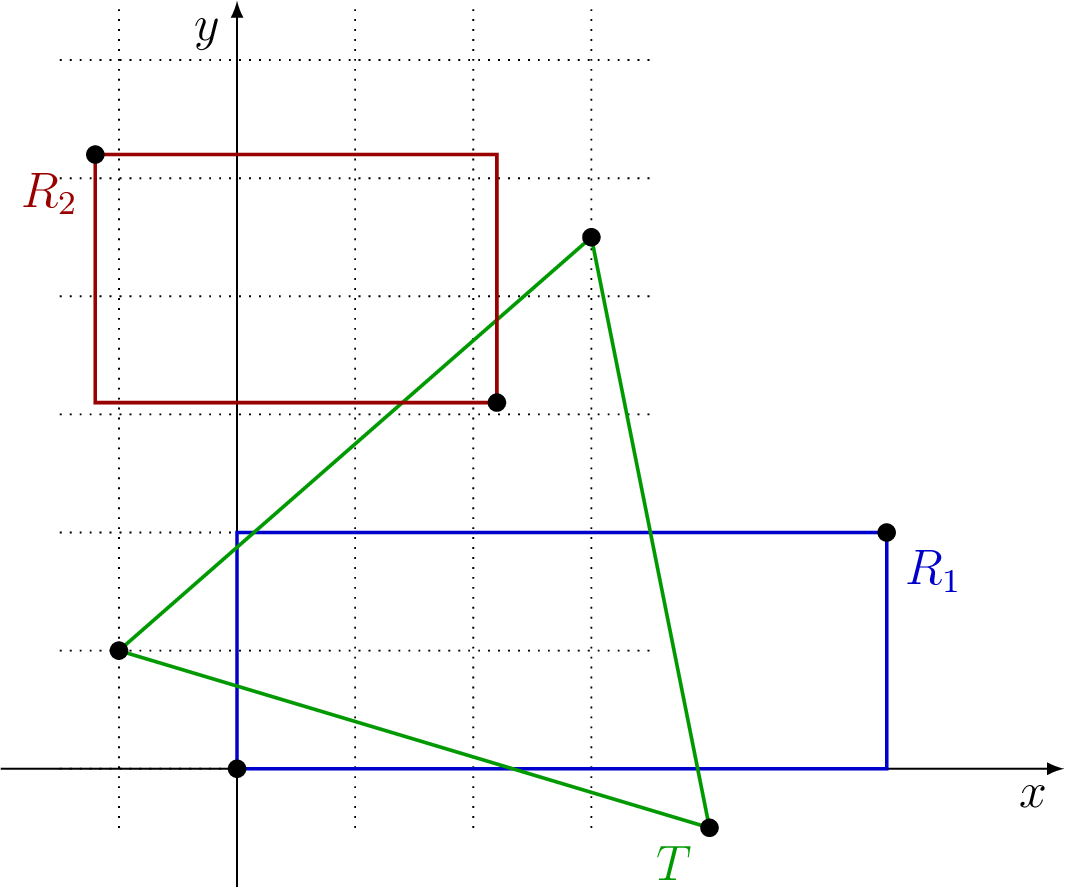
\includegraphics[width=0.6\linewidth,height=\textheight,keepaspectratio]{figuras/retangulos-e-triangulos.png}

}

\end{figure}%

Uma solução para processar os dados desse arquivo e apresentar as áreas
de cada figura é o
Algoritmo~\ref{alg-retangulos-e-triangulos-com-prefixacao}, apresentado
com nível alto de abstração.

\begin{algorithm}[H]
\caption{\label{alg-retangulos-e-triangulos-com-prefixacao}Processamento
de formas em arquivo com apresentação das suas áreas, com prefixação do
número de formas.}
\begingroup%

%| title: Processamento de formas em arquivo com apresentação das suas áreas, com prefixação do número de formas.
%| label: #alg-retangulos-e-triangulos-com-prefixacao

\begin{algorithmic}
    \Description Processamento de um arquivo de formas (triângulos e retângulos) para cálculo das áreas
    \Require arquivo texto com número de formas seguido de uma forma por linha: triângulo (letra T mais coordenadas de seus três vértices) ou retângulo (letra R e as coordenadas de dois vértices opostos)
    \Ensure a apresentação da área de cada forma
    \Statex{}
    \State{Obtenha \Id{número\_formas} do arquivo}
    \For{$i \gets 1$ \To \Id{número\_formas}}[primeira linha]
        \Statep{Obtenha uma forma}[uma linha]
        \If{a forma é um triângulo}
            \Statep{Calcule a área por semiperímetro}[triângulo]
        \Else
            \Statep{Calcule a área como base multiplicada por altura}[retângulo]
        \EndIf
        \Statep{apresente a área calculada}
    \EndFor
\end{algorithmic}

\endgroup
\end{algorithm}

A implementação desse algoritmo em C pode ser feita conforme o programa
seguinte. Nessa codificação, o arquivo lógico é dado pela variável
\texttt{arquivo\_formas}, associado ao arquivo físico
\texttt{figuras.txt}.

\begin{Shaded}
\begin{Highlighting}[]
\CommentTok{/*}
\CommentTok{Processamento de um arquivo de formas (triângulos e retângulos) para cálculo}
\CommentTok{    das áreas}
\CommentTok{Requer: arquivo texto com nome \textquotesingle{}figuras.txt\textquotesingle{}:}
\CommentTok{    na linha 1: número de formas}
\CommentTok{    nas linhas restantes, conforme a quantidade da linha 1:}
\CommentTok{        {-} OU a letra T mais coordenadas dos vértices do triângulo}
\CommentTok{        {-} OU a letra R e as coordenadas de dois vértices opostos do}
\CommentTok{            retângulo}
\CommentTok{Assegura: a apresentação da área de cada forma}
\CommentTok{*/}
\PreprocessorTok{\#include }\ImportTok{\textless{}stdio.h\textgreater{}}
\PreprocessorTok{\#include }\ImportTok{\textless{}math.h\textgreater{}}

\DataTypeTok{int}\NormalTok{ main}\OperatorTok{(}\DataTypeTok{void}\OperatorTok{)} \OperatorTok{\{}
    \DataTypeTok{FILE} \OperatorTok{*}\NormalTok{arquivo\_formas }\OperatorTok{=}\NormalTok{ fopen}\OperatorTok{(}\StringTok{"figuras.txt"}\OperatorTok{,} \StringTok{"r"}\OperatorTok{);}

    \ControlFlowTok{if} \OperatorTok{(}\NormalTok{arquivo\_formas }\OperatorTok{==}\NormalTok{ NULL}\OperatorTok{)} \OperatorTok{\{}
\NormalTok{        printf}\OperatorTok{(}\StringTok{"Falha ao abrir arquivo de formas.}\SpecialCharTok{\textbackslash{}n}\StringTok{"}\OperatorTok{);}
    \OperatorTok{\}}
    \ControlFlowTok{else} \OperatorTok{\{}
        \DataTypeTok{char}\NormalTok{ entrada}\OperatorTok{[}\DecValTok{160}\OperatorTok{];}
\NormalTok{        fgets}\OperatorTok{(}\NormalTok{entrada}\OperatorTok{,} \KeywordTok{sizeof}\NormalTok{ entrada}\OperatorTok{,}\NormalTok{ arquivo\_formas}\OperatorTok{);}
        \DataTypeTok{int}\NormalTok{ numero\_formas}\OperatorTok{;}
\NormalTok{        sscanf}\OperatorTok{(}\NormalTok{entrada}\OperatorTok{,} \StringTok{"}\SpecialCharTok{\%d}\StringTok{"}\OperatorTok{,} \OperatorTok{\&}\NormalTok{numero\_formas}\OperatorTok{);}

        \CommentTok{// Processamento das formas}
        \ControlFlowTok{for} \OperatorTok{(}\DataTypeTok{int}\NormalTok{ i }\OperatorTok{=} \DecValTok{0}\OperatorTok{;}\NormalTok{ i }\OperatorTok{\textless{}}\NormalTok{ numero\_formas}\OperatorTok{;}\NormalTok{ i}\OperatorTok{++)} \OperatorTok{\{}
            \CommentTok{// Obtenção da linha com a forma}
\NormalTok{            fgets}\OperatorTok{(}\NormalTok{entrada}\OperatorTok{,} \KeywordTok{sizeof}\NormalTok{ entrada}\OperatorTok{,}\NormalTok{ arquivo\_formas}\OperatorTok{);}
            \DataTypeTok{double}\NormalTok{ area}\OperatorTok{;}
            \ControlFlowTok{if} \OperatorTok{(}\NormalTok{entrada}\OperatorTok{[}\DecValTok{0}\OperatorTok{]} \OperatorTok{==} \CharTok{\textquotesingle{}T\textquotesingle{}}\OperatorTok{)} \OperatorTok{\{}
                \CommentTok{// Triângulo: área por semiperímetro}
                \DataTypeTok{double}\NormalTok{ x1}\OperatorTok{,}\NormalTok{ y1}\OperatorTok{,}\NormalTok{ x2}\OperatorTok{,}\NormalTok{ y2}\OperatorTok{,}\NormalTok{ x3}\OperatorTok{,}\NormalTok{ y3}\OperatorTok{;}
\NormalTok{                sscanf}\OperatorTok{(}\NormalTok{entrada}\OperatorTok{,} \StringTok{"}\SpecialCharTok{\%*c\%lf\%lf\%lf\%lf\%lf\%lf}\StringTok{"}\OperatorTok{,}
                       \OperatorTok{\&}\NormalTok{x1}\OperatorTok{,} \OperatorTok{\&}\NormalTok{y1}\OperatorTok{,} \OperatorTok{\&}\NormalTok{x2}\OperatorTok{,} \OperatorTok{\&}\NormalTok{y2}\OperatorTok{,} \OperatorTok{\&}\NormalTok{x3}\OperatorTok{,} \OperatorTok{\&}\NormalTok{y3}\OperatorTok{);}
                \DataTypeTok{double}\NormalTok{ lado1 }\OperatorTok{=}\NormalTok{ sqrt}\OperatorTok{(}\NormalTok{pow}\OperatorTok{(}\NormalTok{x1 }\OperatorTok{{-}}\NormalTok{ x2}\OperatorTok{,} \DecValTok{2}\OperatorTok{)} \OperatorTok{+}\NormalTok{ pow}\OperatorTok{(}\NormalTok{y1 }\OperatorTok{{-}}\NormalTok{ y2}\OperatorTok{,} \DecValTok{2}\OperatorTok{));}
                \DataTypeTok{double}\NormalTok{ lado2 }\OperatorTok{=}\NormalTok{ sqrt}\OperatorTok{(}\NormalTok{pow}\OperatorTok{(}\NormalTok{x1 }\OperatorTok{{-}}\NormalTok{ x3}\OperatorTok{,} \DecValTok{2}\OperatorTok{)} \OperatorTok{+}\NormalTok{ pow}\OperatorTok{(}\NormalTok{y1 }\OperatorTok{{-}}\NormalTok{ y3}\OperatorTok{,} \DecValTok{2}\OperatorTok{));}
                \DataTypeTok{double}\NormalTok{ lado3 }\OperatorTok{=}\NormalTok{ sqrt}\OperatorTok{(}\NormalTok{pow}\OperatorTok{(}\NormalTok{x2 }\OperatorTok{{-}}\NormalTok{ x3}\OperatorTok{,} \DecValTok{2}\OperatorTok{)} \OperatorTok{+}\NormalTok{ pow}\OperatorTok{(}\NormalTok{y2 }\OperatorTok{{-}}\NormalTok{ y3}\OperatorTok{,} \DecValTok{2}\OperatorTok{));}
                \DataTypeTok{double}\NormalTok{ semiperimetro }\OperatorTok{=} \OperatorTok{(}\NormalTok{lado1 }\OperatorTok{+}\NormalTok{ lado2 }\OperatorTok{+}\NormalTok{ lado3}\OperatorTok{)} \OperatorTok{/} \DecValTok{2}\OperatorTok{;}

\NormalTok{                area }\OperatorTok{=}\NormalTok{ sqrt}\OperatorTok{(}\NormalTok{semiperimetro }\OperatorTok{*} \OperatorTok{(}\NormalTok{semiperimetro }\OperatorTok{{-}}\NormalTok{ lado1}\OperatorTok{)} \OperatorTok{*}
                            \OperatorTok{(}\NormalTok{semiperimetro }\OperatorTok{{-}}\NormalTok{ lado2}\OperatorTok{)} \OperatorTok{*} \OperatorTok{(}\NormalTok{semiperimetro }\OperatorTok{{-}}\NormalTok{ lado3}\OperatorTok{));}
            \OperatorTok{\}}
            \ControlFlowTok{else} \OperatorTok{\{}
                \CommentTok{// Retângulo: ára por base x altura}
                \DataTypeTok{double}\NormalTok{ x1}\OperatorTok{,}\NormalTok{ y1}\OperatorTok{,}\NormalTok{ x2}\OperatorTok{,}\NormalTok{ y2}\OperatorTok{;}
\NormalTok{                sscanf}\OperatorTok{(}\NormalTok{entrada}\OperatorTok{,} \StringTok{"}\SpecialCharTok{\%*c\%lf\%lf\%lf\%lf}\StringTok{"}\OperatorTok{,} \OperatorTok{\&}\NormalTok{x1}\OperatorTok{,} \OperatorTok{\&}\NormalTok{y1}\OperatorTok{,} \OperatorTok{\&}\NormalTok{x2}\OperatorTok{,} \OperatorTok{\&}\NormalTok{y2}\OperatorTok{);}

\NormalTok{                area }\OperatorTok{=}\NormalTok{ fabs}\OperatorTok{(}\NormalTok{x2 }\OperatorTok{{-}}\NormalTok{ x1}\OperatorTok{)} \OperatorTok{*}\NormalTok{ fabs}\OperatorTok{(}\NormalTok{y2 }\OperatorTok{{-}}\NormalTok{ y1}\OperatorTok{);}
            \OperatorTok{\}}

\NormalTok{            printf}\OperatorTok{(}\StringTok{"}\SpecialCharTok{\%.2f\textbackslash{}n}\StringTok{"}\OperatorTok{,}\NormalTok{ area}\OperatorTok{);}
        \OperatorTok{\}}

\NormalTok{        fclose}\OperatorTok{(}\NormalTok{arquivo\_formas}\OperatorTok{);}
    \OperatorTok{\}}

    \ControlFlowTok{return} \DecValTok{0}\OperatorTok{;}
\OperatorTok{\}}
\end{Highlighting}
\end{Shaded}

\begin{Shaded}
\begin{Highlighting}[]
\NormalTok{11.00}
\NormalTok{11.75}
\NormalTok{7.14}
\end{Highlighting}
\end{Shaded}

A função \texttt{fopen} usa como parâmetros o nome do arquivo de formas
e o modo \texttt{"r"}, que indica acesso para leitura. Todas as leituras
são feitas linha a linha, usando a variável genérica \texttt{entrada}
para armazenamento temporário. Para o caso da primeira linha, a qual
contém apenas a quantidade de formas do arquivo, esse valor é obtido
pelo \texttt{sscanf} usando-se o formato \texttt{\%d}.

No caso das linhas de cada forma, cada uma delas é armazenada em
\texttt{entrada}, porém analisadas de forma diferente. Como o primeiro
caractere da linha indica sua forma, a decisão entre triângulo e
retângulo é feita com base em \texttt{entrada{[}0{]}}, que será
\texttt{T} ou \texttt{R}.

Com base no tipo da forma, a linha é analisada de forma separada. No
caso do triângulo, são esperados seis valores que formam as três
coordenadas dos vértices e, desse modo, o \texttt{sscanf} usa o padrão
de formato \texttt{\%*c\%lf\%lf\%lf\%lf}, que ignora o primeiro
caractere e faz a varredura procurando seis valores reais. Para o caso
do retângulo, no qual há apenas dois pontos, o padrão usado é
\texttt{\%*c\%lf\%lf\%lf\%lf}, o qual ignora o \texttt{R} e obtém os
quatro valores que formam as duas coordenadas dos vértices opostos.

Naturalmente, terminado o processamento do arquivo, \texttt{fclose} é
usado para liberar o sistema operacional de gerenciar o arquivo de
dados.

\section{Mais sobre a abertura e o fechamento de arquivos
texto}\label{mais-sobre-a-abertura-e-o-fechamento-de-arquivos-texto}

Nesta seção são reapresentadas as funções de manipulação de arquivos com
mais detalhamento sobre seu funcionamento e uso dos parâmetros.

\subsection{\texorpdfstring{A função
\texttt{fopen}}{A função fopen}}\label{a-funuxe7uxe3o-fopen}

A função de associação entre o programa e o arquivo real é a
\texttt{fopen}. Ela sempre possui dois parâmetros, sendo o primeiro a
indicação do nome do arquivo e o segundo, o modo de abertura.

O nome do arquivo é uma cadeia de caracteres que pode ser somente o nome
do arquivo, como \texttt{"figuras.txt"}, por exemplo. Nesse caso, o
arquivo físico é considerado em relação ao diretório corrente. O nome
pode indicar também o caminho: \texttt{"../figuras.txt"} indica o
arquivo no diretório pai (isto é, um acima do atual) e
\texttt{"/home/user/dados/figuras.txt"} dá o caminho absoluto e
independe do diretório corrente\footnote{No Linux, usado como plataforma
  para este livro, o separador de diretórios é a barra \texttt{/}. O
  mesmo ocorre para o MacOS. Em sistemas Windows, os caminhos usam a
  barra reversa \texttt{\textbackslash{}} e, como essa barra tem
  significado especial em C, é preciso indicar o caminho com o escape
  \texttt{\textbackslash{}\textbackslash{}}:
  \texttt{"..\textbackslash{}\textbackslash{}figuras.txt"} ou
  \texttt{C:\textbackslash{}\textbackslash{}User\textbackslash{}\textbackslash{}Documentos\textbackslash{}\textbackslash{}Dados\textbackslash{}\textbackslash{}figuras.txt}.}.

Em relação aos modos, como \texttt{"w"} ou \texttt{"r"} usados nos
exemplos, a Tabela~\ref{tbl-modos-arquivo-texto} sumariza como
funcionam.

\begin{longtable}[]{@{}
  >{\centering\arraybackslash}p{(\linewidth - 2\tabcolsep) * \real{0.0889}}
  >{\raggedright\arraybackslash}p{(\linewidth - 2\tabcolsep) * \real{0.9111}}@{}}
\caption{Modos do \texttt{fopen} para manipulação de arquivos
texto.}\label{tbl-modos-arquivo-texto}\tabularnewline
\toprule\noalign{}
\begin{minipage}[b]{\linewidth}\centering
{~~Modo~~}
\end{minipage} & \begin{minipage}[b]{\linewidth}\raggedright
Significado
\end{minipage} \\
\midrule\noalign{}
\endfirsthead
\toprule\noalign{}
\begin{minipage}[b]{\linewidth}\centering
{~~Modo~~}
\end{minipage} & \begin{minipage}[b]{\linewidth}\raggedright
Significado
\end{minipage} \\
\midrule\noalign{}
\endhead
\bottomrule\noalign{}
\endlastfoot
\texttt{"w"} & Prepara um arquivo somente para escrita, criando um
arquivo novo ou truncando o existente para tamanho zero. A posição
corrente é ajustada para o início do arquivo. \\
\texttt{"r"} & Prepara um arquivo somente para leitura. A posição
corrente é ajustada para o início do arquivo. \\
\texttt{"a"} & Prepara um arquivo somente para escrita. Se o arquivo já
existir, a posição corrente é ajustada para o final do arquivo; senão,
um novo arquivo é criado. \\
\end{longtable}

Arquivos texto são, via de regra, processados sequencialmente, do início
ao fim ou do início até um ponto de interesse qualquer. Raramente são
abertos para leitura e escrita, de forma que essa opção foi omitida da
lista apresentada.

A Tabela~\ref{tbl-modos-arquivo-texto} também introduz um elemento
importante, embora intuitivamente fácil de compreender: a posição
corrente. Esse termo é aplicado ao local no arquivo onde as operações de
leitura e escrita serão realizadas. Por exemplo, quando um arquivo é
aberto em modo \texttt{"r"}, a posição corrente está no início do
arquivo, que é o byte zero. A cada leitura, a posição corrente é
ajustada para o próximo byte que será lido.

Embora a posição corrente não seja diretamente usada pelo programador no
processamento sequencial do arquivo, um exemplo simples de programa
ilustra esse conceito.

\begin{Shaded}
\begin{Highlighting}[]
\CommentTok{/*}
\CommentTok{Escrita de algumas linhas de texto em um arquivo com acompanhamento da}
\CommentTok{    posição corrente de Escrita}
\CommentTok{Assegura: criação de arquivo \textquotesingle{}texto.txt\textquotesingle{} com algum texto e apresentação}
\CommentTok{    dos bytes usados em cada linha durante a escrita}
\CommentTok{*/}
\PreprocessorTok{\#include }\ImportTok{\textless{}stdio.h\textgreater{}}

\DataTypeTok{int}\NormalTok{ main}\OperatorTok{(}\DataTypeTok{void}\OperatorTok{)} \OperatorTok{\{}
    \DataTypeTok{FILE} \OperatorTok{*}\NormalTok{arquivo\_numeros }\OperatorTok{=}\NormalTok{ fopen}\OperatorTok{(}\StringTok{"texto.txt"}\OperatorTok{,} \StringTok{"w"}\OperatorTok{);}

    \ControlFlowTok{if} \OperatorTok{(}\NormalTok{arquivo\_numeros }\OperatorTok{==}\NormalTok{ NULL}\OperatorTok{)}
\NormalTok{        printf}\OperatorTok{(}\StringTok{"Falha ao criar arquivo de saída.}\SpecialCharTok{\textbackslash{}n}\StringTok{"}\OperatorTok{);}
    \ControlFlowTok{else} \OperatorTok{\{}
\NormalTok{        printf}\OperatorTok{(}\StringTok{"Primeira linha: bytes de }\SpecialCharTok{\%ld}\StringTok{"}\OperatorTok{,}\NormalTok{ ftell}\OperatorTok{(}\NormalTok{arquivo\_numeros}\OperatorTok{));}
\NormalTok{        fprintf}\OperatorTok{(}\NormalTok{arquivo\_numeros}\OperatorTok{,} \StringTok{"Primeira linha deste arquivo.}\SpecialCharTok{\textbackslash{}n}\StringTok{"}\OperatorTok{);}
\NormalTok{        printf}\OperatorTok{(}\StringTok{" a }\SpecialCharTok{\%ld}\StringTok{.}\SpecialCharTok{\textbackslash{}n}\StringTok{"}\OperatorTok{,}\NormalTok{ ftell}\OperatorTok{(}\NormalTok{arquivo\_numeros}\OperatorTok{)} \OperatorTok{{-}} \DecValTok{1}\OperatorTok{);}

\NormalTok{        printf}\OperatorTok{(}\StringTok{"Segunda linha: bytes de }\SpecialCharTok{\%ld}\StringTok{"}\OperatorTok{,}\NormalTok{ ftell}\OperatorTok{(}\NormalTok{arquivo\_numeros}\OperatorTok{));}
\NormalTok{        fprintf}\OperatorTok{(}\NormalTok{arquivo\_numeros}\OperatorTok{,} \StringTok{"Linha 2"}\OperatorTok{);}  \CommentTok{// escrita em duas etapas}
\NormalTok{        fprintf}\OperatorTok{(}\NormalTok{arquivo\_numeros}\OperatorTok{,} \StringTok{" segue aqui...}\SpecialCharTok{\textbackslash{}n}\StringTok{"}\OperatorTok{);}
\NormalTok{        printf}\OperatorTok{(}\StringTok{" a }\SpecialCharTok{\%ld}\StringTok{.}\SpecialCharTok{\textbackslash{}n}\StringTok{"}\OperatorTok{,}\NormalTok{ ftell}\OperatorTok{(}\NormalTok{arquivo\_numeros}\OperatorTok{)} \OperatorTok{{-}} \DecValTok{1}\OperatorTok{);}

\NormalTok{        printf}\OperatorTok{(}\StringTok{"Terceira linha: bytes de }\SpecialCharTok{\%ld}\StringTok{"}\OperatorTok{,}\NormalTok{ ftell}\OperatorTok{(}\NormalTok{arquivo\_numeros}\OperatorTok{));}
\NormalTok{        fprintf}\OperatorTok{(}\NormalTok{arquivo\_numeros}\OperatorTok{,} \StringTok{"Finalmente o fim do texto! (linha 3)"}\OperatorTok{);}
\NormalTok{        printf}\OperatorTok{(}\StringTok{" a }\SpecialCharTok{\%ld}\StringTok{.}\SpecialCharTok{\textbackslash{}n}\StringTok{"}\OperatorTok{,}\NormalTok{ ftell}\OperatorTok{(}\NormalTok{arquivo\_numeros}\OperatorTok{)} \OperatorTok{{-}} \DecValTok{1}\OperatorTok{);}

\NormalTok{        fclose}\OperatorTok{(}\NormalTok{arquivo\_numeros}\OperatorTok{);}
    \OperatorTok{\}}

    \ControlFlowTok{return} \DecValTok{0}\OperatorTok{;}
\OperatorTok{\}}
\end{Highlighting}
\end{Shaded}

\begin{Shaded}
\begin{Highlighting}[]
\NormalTok{Primeira linha: bytes de 0 a 29.}
\NormalTok{Segunda linha: bytes de 30 a 51.}
\NormalTok{Terceira linha: bytes de 52 a 87.}
\end{Highlighting}
\end{Shaded}

O conteúdo de \texttt{texto.txt} ficou como se segue.

\begin{Shaded}
\begin{Highlighting}[]
\NormalTok{Primeira linha deste arquivo.}
\NormalTok{Linha 2 segue aqui...}
\NormalTok{Finalmente o fim do texto! (linha 3)}
\end{Highlighting}
\end{Shaded}

Para visualização, a seguir é apresentado o conteúdo do arquivo com
16~bytes por linha. A primeira coluna é a contagem de caracteres
(primeira linha do \texttt{od} são os bytes de zero a 15), o que ajuda a
identificar a posição de cada caractere relativo a sua posição do
arquivo. Os valores \texttt{\textbackslash{}n} são as mudanças de linha
usuais\footnote{No Windows, a mudança de linha costuma ser indicada pela
  sequência \texttt{\textbackslash{}r\textbackslash{}n}, de modo que o
  conteúdo do arquivo pode diferir um pouco caso seja essa a plataforma
  usada para execução do programa.}. Vale a pena confrontar os valores
escritos pelo programa anterior com as posições reais do arquivo.

\begin{Shaded}
\begin{Highlighting}[]
\NormalTok{$ }\KeywordTok{od {-}Ad {-}tc texto.txt}
\NormalTok{0000000   P   r   i   m   e   i   r   a       l   i   n   h   a       d}
\NormalTok{0000016   e   s   t   e       a   r   q   u   i   v   o   .  \textbackslash{}n   L   i}
\NormalTok{0000032   n   h   a       2       s   e   g   u   e       a   q   u   i}
\NormalTok{0000048   .   .   .  \textbackslash{}n   F   i   n   a   l   m   e   n   t   e       o}
\NormalTok{0000064       f   i   m       d   o       t   e   x   t   o   !       (}
\NormalTok{0000080   l   i   n   h   a       3   )}
\NormalTok{0000088}
\end{Highlighting}
\end{Shaded}

O conceito da posição corrente também é válido para as leituras, que se
iniciam na posição zero (início do arquivo) e, após cada leitura, é
atualizada para o próximo byte que será lido em um próximo
\texttt{fgets}.

A ideia da posição em que ocorre a próxima operação de entrada ou saída
é a usada quando o modo \texttt{"a"} é usado no \texttt{fopen}. Nesse
caso, o arquivo é aberto para escrita, seu conteúdo (se existir) é
preservado e a posição corrente é colocada depois do último byte do
arquivo. Com isso, uma nova escrita no arquivo acrescentará texto ao seu
final.

Um \emph{log} é um arquivo usado para registrar eventos. Por exemplo,
sempre que um usuário entra no sistema ou quando um trabalho de
impressão é iniciado, cada evento é registrado no \emph{log}. O programa
seguinte, cada vez que executado, solicita uma linha de informação e a
grava em um arquivo de \emph{log}.

\begin{Shaded}
\begin{Highlighting}[]
\CommentTok{/*}
\CommentTok{Inserção de uma linha no arquivo de log \textquotesingle{}registro.log\textquotesingle{}}
\CommentTok{Requer: a digitação da linha de informação}
\CommentTok{Assegura: o acréscimo dessa linha no final do arquivo}
\CommentTok{*/}
\PreprocessorTok{\#include }\ImportTok{\textless{}stdio.h\textgreater{}}

\DataTypeTok{int}\NormalTok{ main}\OperatorTok{(}\DataTypeTok{void}\OperatorTok{)} \OperatorTok{\{}
    \DataTypeTok{FILE} \OperatorTok{*}\NormalTok{arquivo\_log }\OperatorTok{=}\NormalTok{ fopen}\OperatorTok{(}\StringTok{"registro.log"}\OperatorTok{,} \StringTok{"a"}\OperatorTok{);}

    \ControlFlowTok{if} \OperatorTok{(}\NormalTok{arquivo\_log }\OperatorTok{==}\NormalTok{ NULL}\OperatorTok{)}
\NormalTok{        printf}\OperatorTok{(}\StringTok{"Falha ao criar ou abrir arquivo de log.}\SpecialCharTok{\textbackslash{}n}\StringTok{"}\OperatorTok{);}
    \ControlFlowTok{else} \OperatorTok{\{}
\NormalTok{        printf}\OperatorTok{(}\StringTok{"Digite a informação a ser registrada:}\SpecialCharTok{\textbackslash{}n}\StringTok{\textgreater{} "}\OperatorTok{);}
        \DataTypeTok{char}\NormalTok{ linha\_de\_log}\OperatorTok{[}\DecValTok{160}\OperatorTok{];}
\NormalTok{        fgets}\OperatorTok{(}\NormalTok{linha\_de\_log}\OperatorTok{,} \KeywordTok{sizeof}\NormalTok{ linha\_de\_log}\OperatorTok{,}\NormalTok{ stdin}\OperatorTok{);}

\NormalTok{        fprintf}\OperatorTok{(}\NormalTok{arquivo\_log}\OperatorTok{,} \StringTok{"}\SpecialCharTok{\%s}\StringTok{"}\OperatorTok{,}\NormalTok{ linha\_de\_log}\OperatorTok{);}

\NormalTok{        fclose}\OperatorTok{(}\NormalTok{arquivo\_log}\OperatorTok{);}
    \OperatorTok{\}}

    \ControlFlowTok{return} \DecValTok{0}\OperatorTok{;}
\OperatorTok{\}}
\end{Highlighting}
\end{Shaded}

\begin{Shaded}
\begin{Highlighting}[]
\NormalTok{Digite a informação a ser registrada:}
\NormalTok{\textgreater{} }\KeywordTok{Primeiro registro do log.}
\end{Highlighting}
\end{Shaded}

Na primeira execução, o arquivo \texttt{registro.log} ainda não existe,
o que faz com que ele seja criado vazio. Então o programa solicita o
primeiro registro e o grava no arquivo.

A cada nova execução, uma linha é solicitada e adicionada ao final do
arquivo.

\begin{tcolorbox}[enhanced jigsaw, arc=.35mm, bottomtitle=1mm, colbacktitle=quarto-callout-warning-color!10!white, title=\textcolor{quarto-callout-warning-color}{\faExclamationTriangle}\hspace{0.5em}{Curiosidade}, toprule=.15mm, left=2mm, opacityback=0, colback=white, colframe=quarto-callout-warning-color-frame, opacitybacktitle=0.6, bottomrule=.15mm, leftrule=.75mm, toptitle=1mm, coltitle=black, titlerule=0mm, rightrule=.15mm, breakable]

Quando um arquivo é aberto apenas para escrita (\texttt{"w"} e
\texttt{"a"}), tentativas de leitura desse arquivo são apenas ignoradas
sem gerar qualquer erro. De forma similar, ao se tentar escrever em um
arquivo aberto com \texttt{"r"}, a escrita não é feita e nenhum erro é
indicado.

\end{tcolorbox}

\subsection{\texorpdfstring{A função
\texttt{fclose}}{A função fclose}}\label{a-funuxe7uxe3o-fclose}

O encerramento do acesso ao arquivo é feito pela função \texttt{fclose},
para a qual é preciso passar como parâmetro a variável correspondente a
um arquivo aberto com sucesso. Uma vez fechado, nenhuma operação de
entrada ou saída para o arquivo é possível.

\section{\texorpdfstring{A função
\texttt{fprintf}}{A função fprintf}}\label{a-funuxe7uxe3o-fprintf}

\index{fprintf@\texttt{fprintf}|textbf} A escrita em um arquivo texto
com o \texttt{fprint} funciona de forma similar ao \texttt{print} na
tela. A função, inicialmente, processa a cadeia de caracteres de formato
e faz as conversões de formato, gerando o texto final. Então, esse texto
é gravado no arquivo. Enquanto \texttt{print} é sempre direcionado para
\emph{stdout}, \texttt{fprintf} permite escolher a qual fluxo de saída o
texto será enviado.

Como exemplo, pode ser considerado o programa seguinte, que cria um
arquivo com algumas operações com raiz quadrada.

\begin{Shaded}
\begin{Highlighting}[]
\CommentTok{/*}
\CommentTok{Criação de arquivo com valores de raízes quadradas}
\CommentTok{Assegura: criação de arquivo texto contendo valores de raízes}
\CommentTok{*/}
\PreprocessorTok{\#include }\ImportTok{\textless{}stdio.h\textgreater{}}
\PreprocessorTok{\#include }\ImportTok{\textless{}math.h\textgreater{}}

\DataTypeTok{int}\NormalTok{ main}\OperatorTok{(}\DataTypeTok{void}\OperatorTok{)} \OperatorTok{\{}
    \DataTypeTok{FILE} \OperatorTok{*}\NormalTok{arquivo\_raizes }\OperatorTok{=}\NormalTok{ fopen}\OperatorTok{(}\StringTok{"raizes.txt"}\OperatorTok{,} \StringTok{"w"}\OperatorTok{);}

    \ControlFlowTok{if} \OperatorTok{(}\NormalTok{arquivo\_raizes }\OperatorTok{==}\NormalTok{ NULL}\OperatorTok{)}
\NormalTok{        printf}\OperatorTok{(}\StringTok{"Falha ao criar arquivo.}\SpecialCharTok{\textbackslash{}n}\StringTok{"}\OperatorTok{);}
    \ControlFlowTok{else} \OperatorTok{\{}
        \ControlFlowTok{for} \OperatorTok{(}\DataTypeTok{double}\NormalTok{ x }\OperatorTok{=} \FloatTok{0.0}\OperatorTok{;}\NormalTok{ x }\OperatorTok{\textless{}=} \DecValTok{100}\OperatorTok{;}\NormalTok{ x }\OperatorTok{+=} \FloatTok{0.5}\OperatorTok{)}
\NormalTok{            fprintf}\OperatorTok{(}\NormalTok{arquivo\_raizes}\OperatorTok{,} \StringTok{"raiz(}\SpecialCharTok{\%.1f}\StringTok{) = }\SpecialCharTok{\%.3f\textbackslash{}n}\StringTok{"}\OperatorTok{,}\NormalTok{ x}\OperatorTok{,}\NormalTok{ sqrt}\OperatorTok{(}\NormalTok{x}\OperatorTok{));}

\NormalTok{        fclose}\OperatorTok{(}\NormalTok{arquivo\_raizes}\OperatorTok{);}
    \OperatorTok{\}}

    \ControlFlowTok{return} \DecValTok{0}\OperatorTok{;}
\OperatorTok{\}}
\end{Highlighting}
\end{Shaded}

O arquivo resultante da execução, \texttt{raizes.txt}, segue.

\begin{Shaded}
\begin{Highlighting}[]
\NormalTok{raiz(0.0) = 0.000}
\NormalTok{raiz(0.5) = 0.707}
\NormalTok{raiz(1.0) = 1.000}
\NormalTok{raiz(1.5) = 1.225}
\NormalTok{raiz(2.0) = 1.414}

\NormalTok{... [191 linhas omitidas]}

\NormalTok{raiz(98.0) = 9.899}
\NormalTok{raiz(98.5) = 9.925}
\NormalTok{raiz(99.0) = 9.950}
\NormalTok{raiz(99.5) = 9.975}
\NormalTok{raiz(100.0) = 10.000}
\end{Highlighting}
\end{Shaded}

Executada uma chamada de \texttt{fprint}, a escrita é feita a partir da
posição corrente, a qual é atualizada para o próximo byte depois do
último byte escrito.

\section{Leitura até o fim do
arquivo}\label{leitura-atuxe9-o-fim-do-arquivo}

Quando um arquivo contém dados, além da estratégia de prefixar os dados
com a quantidade (estratégia usada no
Algoritmo~\ref{alg-retangulos-e-triangulos-com-prefixacao}), é também
possível varrer o arquivo até encontrar seu final. O
Algoritmo~\ref{alg-retangulos-e-triangulos-sem-prefixacao} aborda esse
novo problema, ainda no contexto de um arquivo com formas triangulares e
retangulares.

\begin{algorithm}[H]
\caption{\label{alg-retangulos-e-triangulos-sem-prefixacao}Processamento
de formas em arquivo com apresentação das suas áreas, com uma forma por
linha.}
\begingroup%

%| title: Processamento de formas em arquivo com apresentação das suas áreas, com uma forma por linha.
%| label: #alg-retangulos-e-triangulos-sem-prefixacao

\begin{algorithmic}
    \Description Processamento de um arquivo de formas (triângulos e retângulos) para cálculo das áreas
    \Require arquivo texto contendo uma forma por linha: triângulo (letra T mais coordenadas de seus três vértices) ou retângulo (letra R e as coordenadas de dois vértices opostos)
    \Ensure a apresentação da área de cada forma
    \Statex{}
    \While{existem formas no arquivo}
        \Statep{Obtenha uma forma}[uma linha]
        \If{a forma é um triângulo}
            \Statep{Calcule a área por semiperímetro}[triângulo]
        \Else
            \Statep{Calcule a área como base multiplicada por altura}[retângulo]
        \EndIf
        \Statep{apresente a área calculada}
    \EndWhile
\end{algorithmic}

\endgroup
\end{algorithm}

A função \texttt{fgets} opera da mesma forma para um arquivo aberto
quanto para \texttt{stdin}, ou seja, os dados do arquivo são lidos para
uma variável do programa até que seja encontrado um final de linha
(\texttt{\textbackslash{}n}). O efeito prático é a leitura de uma linha
por vez.

Quando não há mais dados no arquivo para serem lidos, situação em que o
fim do arquivo foi atingido, o valor de retorno de \texttt{fgets} é
\texttt{NULL}. Assim, pela verificação do valor de retorno, é possível
verificar se se chegou ao fim dos dados.

O programa em C seguinte implementa do
Algoritmo~\ref{alg-retangulos-e-triangulos-sem-prefixacao}, verificando
se ainda há formas do arquivo analisando o valor de retorno de
\texttt{fgets}.

\begin{Shaded}
\begin{Highlighting}[]
\CommentTok{/*}
\CommentTok{Processamento de um arquivo de formas (triângulos e retângulos) para cálculo}
\CommentTok{    das áreas}
\CommentTok{Requer: arquivo texto com nome \textquotesingle{}figuras.txt\textquotesingle{} com cada linha contendo:}
\CommentTok{        {-} OU a letra T mais coordenadas dos vértices do triângulo}
\CommentTok{        {-} OU a letra R e as coordenadas de dois vértices opostos do}
\CommentTok{            retângulo}
\CommentTok{Assegura: a apresentação da área de cada forma}
\CommentTok{*/}
\PreprocessorTok{\#include }\ImportTok{\textless{}stdio.h\textgreater{}}
\PreprocessorTok{\#include }\ImportTok{\textless{}math.h\textgreater{}}

\DataTypeTok{int}\NormalTok{ main}\OperatorTok{(}\DataTypeTok{void}\OperatorTok{)} \OperatorTok{\{}
    \DataTypeTok{FILE} \OperatorTok{*}\NormalTok{arquivo\_formas }\OperatorTok{=}\NormalTok{ fopen}\OperatorTok{(}\StringTok{"figuras.txt"}\OperatorTok{,} \StringTok{"r"}\OperatorTok{);}

    \ControlFlowTok{if} \OperatorTok{(}\NormalTok{arquivo\_formas }\OperatorTok{==}\NormalTok{ NULL}\OperatorTok{)} \OperatorTok{\{}
\NormalTok{        printf}\OperatorTok{(}\StringTok{"Falha ao abrir arquivo de formas.}\SpecialCharTok{\textbackslash{}n}\StringTok{"}\OperatorTok{);}
    \OperatorTok{\}}
    \ControlFlowTok{else} \OperatorTok{\{}
        \DataTypeTok{char}\NormalTok{ forma}\OperatorTok{[}\DecValTok{160}\OperatorTok{];}
        \CommentTok{// Obtenção do número de formas}
        \ControlFlowTok{while} \OperatorTok{(}\NormalTok{fgets}\OperatorTok{(}\NormalTok{forma}\OperatorTok{,} \KeywordTok{sizeof}\NormalTok{ forma}\OperatorTok{,}\NormalTok{ arquivo\_formas}\OperatorTok{)} \OperatorTok{!=}\NormalTok{ NULL}\OperatorTok{)} \OperatorTok{\{}
            \DataTypeTok{double}\NormalTok{ area}\OperatorTok{;}
            \ControlFlowTok{if} \OperatorTok{(}\NormalTok{forma}\OperatorTok{[}\DecValTok{0}\OperatorTok{]} \OperatorTok{==} \CharTok{\textquotesingle{}T\textquotesingle{}}\OperatorTok{)} \OperatorTok{\{}
                \CommentTok{// Triângulo: área por semiperímetro}
                \DataTypeTok{double}\NormalTok{ x1}\OperatorTok{,}\NormalTok{ y1}\OperatorTok{,}\NormalTok{ x2}\OperatorTok{,}\NormalTok{ y2}\OperatorTok{,}\NormalTok{ x3}\OperatorTok{,}\NormalTok{ y3}\OperatorTok{;}
\NormalTok{                sscanf}\OperatorTok{(}\NormalTok{forma}\OperatorTok{,} \StringTok{"}\SpecialCharTok{\%*c\%lf\%lf\%lf\%lf\%lf\%lf}\StringTok{"}\OperatorTok{,}
                       \OperatorTok{\&}\NormalTok{x1}\OperatorTok{,} \OperatorTok{\&}\NormalTok{y1}\OperatorTok{,} \OperatorTok{\&}\NormalTok{x2}\OperatorTok{,} \OperatorTok{\&}\NormalTok{y2}\OperatorTok{,} \OperatorTok{\&}\NormalTok{x3}\OperatorTok{,} \OperatorTok{\&}\NormalTok{y3}\OperatorTok{);}
                \DataTypeTok{double}\NormalTok{ lado1 }\OperatorTok{=}\NormalTok{ sqrt}\OperatorTok{(}\NormalTok{pow}\OperatorTok{(}\NormalTok{x1 }\OperatorTok{{-}}\NormalTok{ x2}\OperatorTok{,} \DecValTok{2}\OperatorTok{)} \OperatorTok{+}\NormalTok{ pow}\OperatorTok{(}\NormalTok{y1 }\OperatorTok{{-}}\NormalTok{ y2}\OperatorTok{,} \DecValTok{2}\OperatorTok{));}
                \DataTypeTok{double}\NormalTok{ lado2 }\OperatorTok{=}\NormalTok{ sqrt}\OperatorTok{(}\NormalTok{pow}\OperatorTok{(}\NormalTok{x1 }\OperatorTok{{-}}\NormalTok{ x3}\OperatorTok{,} \DecValTok{2}\OperatorTok{)} \OperatorTok{+}\NormalTok{ pow}\OperatorTok{(}\NormalTok{y1 }\OperatorTok{{-}}\NormalTok{ y3}\OperatorTok{,} \DecValTok{2}\OperatorTok{));}
                \DataTypeTok{double}\NormalTok{ lado3 }\OperatorTok{=}\NormalTok{ sqrt}\OperatorTok{(}\NormalTok{pow}\OperatorTok{(}\NormalTok{x2 }\OperatorTok{{-}}\NormalTok{ x3}\OperatorTok{,} \DecValTok{2}\OperatorTok{)} \OperatorTok{+}\NormalTok{ pow}\OperatorTok{(}\NormalTok{y2 }\OperatorTok{{-}}\NormalTok{ y3}\OperatorTok{,} \DecValTok{2}\OperatorTok{));}
                \DataTypeTok{double}\NormalTok{ semiperimetro }\OperatorTok{=} \OperatorTok{(}\NormalTok{lado1 }\OperatorTok{+}\NormalTok{ lado2 }\OperatorTok{+}\NormalTok{ lado3}\OperatorTok{)} \OperatorTok{/} \DecValTok{2}\OperatorTok{;}

\NormalTok{                area }\OperatorTok{=}\NormalTok{ sqrt}\OperatorTok{(}\NormalTok{semiperimetro }\OperatorTok{*} \OperatorTok{(}\NormalTok{semiperimetro }\OperatorTok{{-}}\NormalTok{ lado1}\OperatorTok{)} \OperatorTok{*}
                            \OperatorTok{(}\NormalTok{semiperimetro }\OperatorTok{{-}}\NormalTok{ lado2}\OperatorTok{)} \OperatorTok{*} \OperatorTok{(}\NormalTok{semiperimetro }\OperatorTok{{-}}\NormalTok{ lado3}\OperatorTok{));}
            \OperatorTok{\}}
            \ControlFlowTok{else} \OperatorTok{\{}
                \CommentTok{// Retângulo: ára por base x altura}
                \DataTypeTok{double}\NormalTok{ x1}\OperatorTok{,}\NormalTok{ y1}\OperatorTok{,}\NormalTok{ x2}\OperatorTok{,}\NormalTok{ y2}\OperatorTok{;}
\NormalTok{                sscanf}\OperatorTok{(}\NormalTok{forma}\OperatorTok{,} \StringTok{"}\SpecialCharTok{\%*c\%lf\%lf\%lf\%lf}\StringTok{"}\OperatorTok{,} \OperatorTok{\&}\NormalTok{x1}\OperatorTok{,} \OperatorTok{\&}\NormalTok{y1}\OperatorTok{,} \OperatorTok{\&}\NormalTok{x2}\OperatorTok{,} \OperatorTok{\&}\NormalTok{y2}\OperatorTok{);}

\NormalTok{                area }\OperatorTok{=}\NormalTok{ fabs}\OperatorTok{(}\NormalTok{x2 }\OperatorTok{{-}}\NormalTok{ x1}\OperatorTok{)} \OperatorTok{*}\NormalTok{ fabs}\OperatorTok{(}\NormalTok{y2 }\OperatorTok{{-}}\NormalTok{ y1}\OperatorTok{);}
            \OperatorTok{\}}

\NormalTok{            printf}\OperatorTok{(}\StringTok{"}\SpecialCharTok{\%.2f\textbackslash{}n}\StringTok{"}\OperatorTok{,}\NormalTok{ area}\OperatorTok{);}
        \OperatorTok{\}}

\NormalTok{        fclose}\OperatorTok{(}\NormalTok{arquivo\_formas}\OperatorTok{);}
    \OperatorTok{\}}

    \ControlFlowTok{return} \DecValTok{0}\OperatorTok{;}
\OperatorTok{\}}
\end{Highlighting}
\end{Shaded}

\begin{Shaded}
\begin{Highlighting}[]
\NormalTok{11.00}
\NormalTok{11.75}
\NormalTok{7.14}
\NormalTok{1.00}
\NormalTok{4.00}
\NormalTok{0.50}
\end{Highlighting}
\end{Shaded}

O arquivo \texttt{figuras.txt} processado por esse programa contém o
conteúdo seguinte. Comparativamente ao usado na
Seção~\ref{sec-fluxo-de-leitura}, o formado de descrição de cada forma é
o mesmo, sendo que apenas a primeira linha contendo o número de formas
não existe.

\begin{Shaded}
\begin{Highlighting}[]
\NormalTok{R 0.0 0.0 5.5 2.0}
\NormalTok{T {-}1.0 1.0 3.0 4.5 4 {-}0.5}
\NormalTok{R {-}1.2 5.2 2.2 3.1}
\NormalTok{R 0 0 1 1}
\NormalTok{R {-}1 {-}1 1 1}
\NormalTok{T 0 0 0 1 1 0}
\end{Highlighting}
\end{Shaded}

Durante a execução, o resultado de \texttt{fgets} é checado a cada
início do \texttt{while}, até que retorne \texttt{NULL} e encerre a
repetição. A cada retorno válido, a área correspondente é calculada.

\section{\texorpdfstring{A função
\texttt{rewind}}{A função rewind}}\label{a-funuxe7uxe3o-rewind}

A palavra \emph{rewind} tem aqui o sentido de rebobinar e vem do tempo
em que os arquivos eram mantidos em fitas magnéticas e, para voltar para
o início do arquivo, era necessário retroceder fisicamente o carretel.
Para o contexto atual, rebobinar significa apenas retornar a posição
corrente para o byte zero, ou seja, o primeiro byte do arquivo.

A função \texttt{rewind} tem o significado de retornar o arquivo para a
primeira posição. Isso significa, por exemplo, que se um arquivo tem que
ser processado mais que uma vez, é possível fazer uma varredura até o
final e, então, retornar ao início e fazer nova leitura.

Um uso interessante de \texttt{rewind} é apresentado no
Algoritmo~\ref{alg-notas-maiores-que-a-media}.

\begin{algorithm}[H]
\caption{\label{alg-notas-maiores-que-a-media}Processamento de arquivo
de notas.}
\begingroup%

%| title: Processamento de arquivo de notas.
%| label: #alg-notas-maiores-que-a-media
\begin{algorithmic}
    \Description Processamento de um arquivo contendo notas de provas para determinação da quantidade de notas maiores que a média geral de notas
    \Require um arquivo texto contendo uma nota por linha, com mínimo de uma linha
    \Ensure a apresentação do número de notas maiores que a média de todas as notas
    \Statex{}
    \Statep{\Commentl{Cálculo da média geral}}
    \While{existem nota no arquivo}
        \Statep{Obtenha uma nota}
        \Statep{Acumule a nota em \Id{soma\_notas}}
        \Statep{Conte essa nota usando \Id{contador\_notas}}
    \EndWhile
    \Statep{Calcule a \Id{média} como ${\Id{soma\_notas}/\Id{contador\_notas}}$}
    \Statex
    \Statep{\Commentl{Contagem do número de notas maiores que a média calculada}}
    \Statep{Retorne ao início do arquivo}
    \While{existem nota no arquivo}
        \Statep{Obtenha uma nota}
        \Statep{Conte essa nota em \Id{contador\_maiores} apenas se ela for maior que \Id{média}}
    \EndWhile
    \Statex
    \Statep{\Commentl{Apresentação do resultado}}
    \Statep{Apresente o valor de \Id{contador\_maiores}}
\end{algorithmic}

\endgroup
\end{algorithm}

Esse problema requer duas passadas pelos valores das notas, uma vez que
a contagem dos valores maiores que a média precisa que a média já tenha
sido calculada e, para calcular a média, é preciso ter passado por todos
as notas. Assim, o arquivo é varrido sequencialmente somando-se as notas
e contando quantas são para, em seguida, calcular a média. Em um segundo
passo, o arquivo é varrido novamente desde o início, para, então, contar
a quantidade de notas maiores que a média.

Como arquivo de notas, segue uma possível versão de \texttt{notas.txt}.

\begin{Shaded}
\begin{Highlighting}[]
\NormalTok{5.4}
\NormalTok{3.4}
\NormalTok{5.6}
\NormalTok{9.8}
\NormalTok{5.0}
\NormalTok{3.8}
\NormalTok{4.4}
\NormalTok{4.9}
\NormalTok{2.5}
\NormalTok{4.8}
\NormalTok{4.9}
\end{Highlighting}
\end{Shaded}

A implementação em C para o processamento do arquivo é apresentada na
sequência.

\begin{Shaded}
\begin{Highlighting}[]
\CommentTok{/*}
\CommentTok{Determinação da quantidade de notas maiores que a média geral das notas}
\CommentTok{    em um arquivo de dados}
\CommentTok{Requer: arquivo texto com uma nota por linha}
\CommentTok{Assegura: a apresentação da quantidade notas maiores que a média geral}
\CommentTok{*/}
\PreprocessorTok{\#include }\ImportTok{\textless{}stdio.h\textgreater{}}

\DataTypeTok{int}\NormalTok{ main}\OperatorTok{(}\DataTypeTok{void}\OperatorTok{)} \OperatorTok{\{}
    \DataTypeTok{FILE} \OperatorTok{*}\NormalTok{arquivo\_notas }\OperatorTok{=}\NormalTok{ fopen}\OperatorTok{(}\StringTok{"notas.txt"}\OperatorTok{,} \StringTok{"r"}\OperatorTok{);}

    \ControlFlowTok{if} \OperatorTok{(}\NormalTok{arquivo\_notas }\OperatorTok{==}\NormalTok{ NULL}\OperatorTok{)} \OperatorTok{\{}
\NormalTok{        printf}\OperatorTok{(}\StringTok{"Falha ao abrir arquivo de notas.}\SpecialCharTok{\textbackslash{}n}\StringTok{"}\OperatorTok{);}
    \OperatorTok{\}}
    \ControlFlowTok{else} \OperatorTok{\{}
        \CommentTok{// Cálculo da média geral das notas}
        \DataTypeTok{char}\NormalTok{ entrada}\OperatorTok{[}\DecValTok{160}\OperatorTok{];}
        \DataTypeTok{double}\NormalTok{ soma\_notas }\OperatorTok{=} \DecValTok{0}\OperatorTok{;}
        \DataTypeTok{int}\NormalTok{ contador\_notas }\OperatorTok{=} \DecValTok{0}\OperatorTok{;}
        \ControlFlowTok{while} \OperatorTok{(}\NormalTok{fgets}\OperatorTok{(}\NormalTok{entrada}\OperatorTok{,} \KeywordTok{sizeof}\NormalTok{ entrada}\OperatorTok{,}\NormalTok{ arquivo\_notas}\OperatorTok{)} \OperatorTok{!=}\NormalTok{ NULL}\OperatorTok{)} \OperatorTok{\{}
            \DataTypeTok{double}\NormalTok{ nota}\OperatorTok{;}
\NormalTok{            sscanf}\OperatorTok{(}\NormalTok{entrada}\OperatorTok{,} \StringTok{"}\SpecialCharTok{\%lf}\StringTok{"}\OperatorTok{,} \OperatorTok{\&}\NormalTok{nota}\OperatorTok{);}
\NormalTok{            soma\_notas }\OperatorTok{+=}\NormalTok{ nota}\OperatorTok{;}
\NormalTok{            contador\_notas}\OperatorTok{++;}
        \OperatorTok{\}}
        \DataTypeTok{double}\NormalTok{ media }\OperatorTok{=}\NormalTok{ soma\_notas }\OperatorTok{/}\NormalTok{ contador\_notas}\OperatorTok{;}

        \CommentTok{// Contagem da quantidade de notas acima da média calculada}
\NormalTok{        rewind}\OperatorTok{(}\NormalTok{arquivo\_notas}\OperatorTok{);}  \CommentTok{// retorna ao início do arquivo}
        \DataTypeTok{int}\NormalTok{ contador\_maiores }\OperatorTok{=} \DecValTok{0}\OperatorTok{;}
        \ControlFlowTok{while} \OperatorTok{(}\NormalTok{fgets}\OperatorTok{(}\NormalTok{entrada}\OperatorTok{,} \KeywordTok{sizeof}\NormalTok{ entrada}\OperatorTok{,}\NormalTok{ arquivo\_notas}\OperatorTok{)} \OperatorTok{!=}\NormalTok{ NULL}\OperatorTok{)} \OperatorTok{\{}
            \DataTypeTok{double}\NormalTok{ nota}\OperatorTok{;}
\NormalTok{            sscanf}\OperatorTok{(}\NormalTok{entrada}\OperatorTok{,} \StringTok{"}\SpecialCharTok{\%lf}\StringTok{"}\OperatorTok{,} \OperatorTok{\&}\NormalTok{nota}\OperatorTok{);}
            \ControlFlowTok{if} \OperatorTok{(}\NormalTok{nota }\OperatorTok{\textgreater{}}\NormalTok{ media}\OperatorTok{)}
\NormalTok{                contador\_maiores}\OperatorTok{++;}
        \OperatorTok{\}}

\NormalTok{        fclose}\OperatorTok{(}\NormalTok{arquivo\_notas}\OperatorTok{);}

        \CommentTok{// Resultado}
\NormalTok{        printf}\OperatorTok{(}\StringTok{"}\SpecialCharTok{\%d}\StringTok{ notas maiores que }\SpecialCharTok{\%.1f}\StringTok{.}\SpecialCharTok{\textbackslash{}n}\StringTok{"}\OperatorTok{,}\NormalTok{ contador\_maiores}\OperatorTok{,}\NormalTok{ media}\OperatorTok{);}
    \OperatorTok{\}}

    \ControlFlowTok{return} \DecValTok{0}\OperatorTok{;}
\OperatorTok{\}}
\end{Highlighting}
\end{Shaded}

\begin{Shaded}
\begin{Highlighting}[]
\NormalTok{4 notas maiores que 5.0.}
\end{Highlighting}
\end{Shaded}

Sem o uso de \texttt{rewind}, o segundo \texttt{while} terminaria de
imediato, visto que a posição corrente já está no fim do arquivo e
qualquer nova leitura retornará \texttt{NULL} como resultado.

\section{\texorpdfstring{A traiçoeira função
\texttt{feof}}{A traiçoeira função feof}}\label{a-traiuxe7oeira-funuxe7uxe3o-feof}

\index{feof@\texttt{feof}} O nome ``\emph{feof}'' é composto pelo
\emph{f} inicial, como (quase) todas as funções que trabalham com
arquivos (\emph{files}), seguido de \emph{eof}, que significa \emph{end
of file}, ou fim de arquivo.

Porém, o uso correto dessa função requer entender tanto o que ela faz e
o que ela não faz. Apesar do nome, \texttt{feof} não verifica se o
arquivo chegou ao fim. Isso é o que ela não faz.

A função \texttt{feof} deve ser usada depois que uma operação de leitura
(\texttt{fgets}, por exemplo) tenta ser executada mas falha. Somente
depois dessa falha é que \texttt{feof} pode ser usada para verificar
porquê a função não foi bem sucedida. Assim, \texttt{feof} volta
verdadeiro quando a razão da falha foi tentar ler além do último dado do
arquivo.

A diferença parece sutil, mas não é. Para entender esse mecanismo, um
programa simples é usado para mostrar o que acontece na leitura de um
arquivo texto e como \texttt{feof} se comporta.

O arquivo usado para exemplo possui apenas duas linhas e é apresentado a
seguir.

\begin{Shaded}
\begin{Highlighting}[]
\NormalTok{Texto da primeira linha}
\NormalTok{E material para a segunda linha!}
\end{Highlighting}
\end{Shaded}

Esse arquivo possui duas linhas, ambas terminadas com
\texttt{\textbackslash{}n}, como pode ser observado ao se analisar mais
detalhadamente o conteúdo do arquivo.

\begin{Shaded}
\begin{Highlighting}[]
\NormalTok{$ }\KeywordTok{od {-}tc {-}Ad texto.txt}
\NormalTok{0000000   T   e   x   t   o       d   a       p   r   i   m   e   i   r}
\NormalTok{0000016   a       l   i   n   h   a  \textbackslash{}n   E       m   a   t   e   r   i}
\NormalTok{0000032   a   l       p   a   r   a       a       s   e   g   u   n   d}
\NormalTok{0000048   a       l   i   n   h   a   !  \textbackslash{}n}
\NormalTok{0000057}
\end{Highlighting}
\end{Shaded}

O programa usado para processar esse arquivo está apresentado na
sequência.

\begin{Shaded}
\begin{Highlighting}[]
\CommentTok{/*}
\CommentTok{Programa exemplo do comportamento da função feof}
\CommentTok{Assegura: a apresentação de informações relevantes ao longo da execução}
\CommentTok{*/}
\PreprocessorTok{\#include }\ImportTok{\textless{}stdio.h\textgreater{}}

\DataTypeTok{int}\NormalTok{ main}\OperatorTok{(}\DataTypeTok{void}\OperatorTok{)} \OperatorTok{\{}
    \DataTypeTok{FILE} \OperatorTok{*}\NormalTok{arquivo }\OperatorTok{=}\NormalTok{ fopen}\OperatorTok{(}\StringTok{"texto.txt"}\OperatorTok{,} \StringTok{"r"}\OperatorTok{);}

    \ControlFlowTok{if} \OperatorTok{(}\NormalTok{arquivo }\OperatorTok{==}\NormalTok{ NULL}\OperatorTok{)}
\NormalTok{        printf}\OperatorTok{(}\StringTok{"Falha ao abrir arquivo com texto."}\OperatorTok{);}
    \ControlFlowTok{else} \OperatorTok{\{}
        \DataTypeTok{char}\NormalTok{ linha}\OperatorTok{[}\DecValTok{160}\OperatorTok{];}

        \CommentTok{// Situação inicial}
\NormalTok{        printf}\OperatorTok{(}\StringTok{"Ao abrir o arquivo: feof = }\SpecialCharTok{\%c}\StringTok{.}\SpecialCharTok{\textbackslash{}n\textbackslash{}n}\StringTok{"}\OperatorTok{,}\NormalTok{ feof}\OperatorTok{(}\NormalTok{arquivo}\OperatorTok{)} \OperatorTok{?} \CharTok{\textquotesingle{}V\textquotesingle{}} \OperatorTok{:} \CharTok{\textquotesingle{}F\textquotesingle{}}\OperatorTok{);}

        \CommentTok{// Primeira leitura}
\NormalTok{        fgets}\OperatorTok{(}\NormalTok{linha}\OperatorTok{,} \KeywordTok{sizeof}\NormalTok{ linha}\OperatorTok{,}\NormalTok{ arquivo}\OperatorTok{);}
\NormalTok{        printf}\OperatorTok{(}\StringTok{"Primeira leitura: }\SpecialCharTok{\%s}\StringTok{"}\OperatorTok{,}\NormalTok{ linha}\OperatorTok{);}
\NormalTok{        printf}\OperatorTok{(}\StringTok{"Depois da 1ª leitura: feof = }\SpecialCharTok{\%c}\StringTok{.}\SpecialCharTok{\textbackslash{}n\textbackslash{}n}\StringTok{"}\OperatorTok{,}
\NormalTok{               feof}\OperatorTok{(}\NormalTok{arquivo}\OperatorTok{)} \OperatorTok{?} \CharTok{\textquotesingle{}V\textquotesingle{}} \OperatorTok{:} \CharTok{\textquotesingle{}F\textquotesingle{}}\OperatorTok{);}

        \CommentTok{// Segunda leitura}
\NormalTok{        fgets}\OperatorTok{(}\NormalTok{linha}\OperatorTok{,} \KeywordTok{sizeof}\NormalTok{ linha}\OperatorTok{,}\NormalTok{ arquivo}\OperatorTok{);}
\NormalTok{        printf}\OperatorTok{(}\StringTok{"Segunda leitura: }\SpecialCharTok{\%s}\StringTok{"}\OperatorTok{,}\NormalTok{ linha}\OperatorTok{);}
\NormalTok{        printf}\OperatorTok{(}\StringTok{"Depois da 2ª leitura: feof = }\SpecialCharTok{\%c}\StringTok{.}\SpecialCharTok{\textbackslash{}n\textbackslash{}n}\StringTok{"}\OperatorTok{,}
\NormalTok{               feof}\OperatorTok{(}\NormalTok{arquivo}\OperatorTok{)} \OperatorTok{?} \CharTok{\textquotesingle{}V\textquotesingle{}} \OperatorTok{:} \CharTok{\textquotesingle{}F\textquotesingle{}}\OperatorTok{);}

        \CommentTok{// Terceira leitura, que deve falhar}
\NormalTok{        fgets}\OperatorTok{(}\NormalTok{linha}\OperatorTok{,} \KeywordTok{sizeof}\NormalTok{ linha}\OperatorTok{,}\NormalTok{ arquivo}\OperatorTok{);}
\NormalTok{        printf}\OperatorTok{(}\StringTok{"Terceira leitura: }\SpecialCharTok{\%s}\StringTok{"}\OperatorTok{,}\NormalTok{ linha}\OperatorTok{);}
\NormalTok{        printf}\OperatorTok{(}\StringTok{"Depois da 3ª leitura: feof = }\SpecialCharTok{\%c}\StringTok{.}\SpecialCharTok{\textbackslash{}n\textbackslash{}n}\StringTok{"}\OperatorTok{,}
\NormalTok{               feof}\OperatorTok{(}\NormalTok{arquivo}\OperatorTok{)} \OperatorTok{?} \CharTok{\textquotesingle{}V\textquotesingle{}} \OperatorTok{:} \CharTok{\textquotesingle{}F\textquotesingle{}}\OperatorTok{);}

\NormalTok{        fclose}\OperatorTok{(}\NormalTok{arquivo}\OperatorTok{);}
    \OperatorTok{\}}
    \ControlFlowTok{return} \DecValTok{0}\OperatorTok{;}
\OperatorTok{\}}
\end{Highlighting}
\end{Shaded}

\begin{Shaded}
\begin{Highlighting}[]
\NormalTok{Ao abrir o arquivo: feof = F.}

\NormalTok{Primeira leitura: Texto da primeira linha}
\NormalTok{Depois da 1ª leitura: feof = F.}

\NormalTok{Segunda leitura: E material para a segunda linha!}
\NormalTok{Depois da 2ª leitura: feof = F.}

\NormalTok{Terceira leitura: E material para a segunda linha!}
\NormalTok{Depois da 3ª leitura: feof = V.}
\end{Highlighting}
\end{Shaded}

Como esperado, as duas primeiras execuções de \texttt{fgets} fazem as
leituras das duas primeiras linhas do arquivo e apresentam seu conteúdo
na tela. Como o arquivo \texttt{texto.txt} possui apenas essas duas
linhas, a terceira chamada a \texttt{fgets} falha, sendo o \texttt{NULL}
retornado ignorado no programa. Como a leitura falha, a variável
\texttt{linha} não é modificada e é por essa razão que a mensagem de
conteúdo da terceira leitura aparece igual ao da segunda.

Quanto à função \texttt{feof}, ela retorna falso (zero) logo ao abrir o
arquivo e também depois da primeira leitura. Na segunda execução de
\texttt{fgets}, a segunda linha é copiada para a variável \texttt{linha}
e efetivamente a posição corrente está no fim do arquivo. Entretanto,
como a leitura não foi além do fim do arquivo, \texttt{feof} ainda
retorna falso. Na terceira leitura, que é mal sucedida por não haver
mais o que ler do arquivo, o \texttt{fgets} não faz a leitura e, a
partir desse momento, \texttt{feof} começa a retornar verdadeiro (valor
não nulo), indicando que o problema foi tentar ler de um arquivo que já
havia terminado.

\begin{tcolorbox}[enhanced jigsaw, arc=.35mm, bottomtitle=1mm, colbacktitle=quarto-callout-caution-color!10!white, title=\textcolor{quarto-callout-caution-color}{\faFire}\hspace{0.5em}{Cuidado}, toprule=.15mm, left=2mm, opacityback=0, colback=white, colframe=quarto-callout-caution-color-frame, opacitybacktitle=0.6, bottomrule=.15mm, leftrule=.75mm, toptitle=1mm, coltitle=black, titlerule=0mm, rightrule=.15mm, breakable]

Por uma tendência em interpretar erroneamente o que \texttt{feof}
realmente verifica, não é incomum programas como o seguinte, que produz
um resultado insatisfatório.

Supondo a existência de um arquvio \texttt{inteiros.txt} com o conteúdo
seguinte, um programa se propõe a fazer a soma dos valores inteiros
contidos nele. Para este arquivo específico, o resultado esperado é 120.

\begin{Shaded}
\begin{Highlighting}[]
\NormalTok{20}
\NormalTok{50}
\NormalTok{30}
\NormalTok{20}
\end{Highlighting}
\end{Shaded}

Este arquivo possui um \texttt{\textbackslash{}n} no final de cada
linha. Como ilustra o comando seguinte.

\begin{Shaded}
\begin{Highlighting}[]
\NormalTok{$ }\KeywordTok{od {-}tc {-}Ad inteiros.txt}
\NormalTok{0000000   2   0  \textbackslash{}n   5   0  \textbackslash{}n   3   0  \textbackslash{}n   2   0  \textbackslash{}n}
\NormalTok{0000012}
\end{Highlighting}
\end{Shaded}

Segue, agora, o programa que tenta processar esse arquivo.

\begin{Shaded}
\begin{Highlighting}[]
\CommentTok{/*}
\CommentTok{Tentativa incorreta de somar os valores de um arquivo de inteiros}
\CommentTok{Requer: um arquivo com valores inteiros, um por linha}
\CommentTok{Assegura: a soma incorreta dos valores}
\CommentTok{*/}
\PreprocessorTok{\#include }\ImportTok{\textless{}stdio.h\textgreater{}}

\DataTypeTok{int}\NormalTok{ main}\OperatorTok{(}\DataTypeTok{void}\OperatorTok{)} \OperatorTok{\{}
    \DataTypeTok{FILE} \OperatorTok{*}\NormalTok{arquivo\_inteiros }\OperatorTok{=}\NormalTok{ fopen}\OperatorTok{(}\StringTok{"inteiros.txt"}\OperatorTok{,} \StringTok{"r"}\OperatorTok{);}

    \ControlFlowTok{if} \OperatorTok{(}\NormalTok{arquivo\_inteiros }\OperatorTok{==}\NormalTok{ NULL}\OperatorTok{)}
\NormalTok{        printf}\OperatorTok{(}\StringTok{"Falha ao abrir arquivo\_inteiros com os valores inteiros."}\OperatorTok{);}
    \ControlFlowTok{else} \OperatorTok{\{}
        \DataTypeTok{int}\NormalTok{ soma }\OperatorTok{=} \DecValTok{0}\OperatorTok{;}
        \ControlFlowTok{while} \OperatorTok{(!}\NormalTok{feof}\OperatorTok{(}\NormalTok{arquivo\_inteiros}\OperatorTok{))} \OperatorTok{\{}
            \CommentTok{// Obtenção do inteiro}
            \DataTypeTok{char}\NormalTok{ entrada}\OperatorTok{[}\DecValTok{160}\OperatorTok{];}
\NormalTok{            fgets}\OperatorTok{(}\NormalTok{entrada}\OperatorTok{,} \KeywordTok{sizeof}\NormalTok{ entrada}\OperatorTok{,}\NormalTok{ arquivo\_inteiros}\OperatorTok{);}
            \DataTypeTok{int}\NormalTok{ valor}\OperatorTok{;}
\NormalTok{            sscanf}\OperatorTok{(}\NormalTok{entrada}\OperatorTok{,} \StringTok{"}\SpecialCharTok{\%d}\StringTok{"}\OperatorTok{,} \OperatorTok{\&}\NormalTok{valor}\OperatorTok{);}

            \CommentTok{// Acumulação do valor}
\NormalTok{            soma }\OperatorTok{+=}\NormalTok{ valor}\OperatorTok{;}
        \OperatorTok{\}}

\NormalTok{        fclose}\OperatorTok{(}\NormalTok{arquivo\_inteiros}\OperatorTok{);}

\NormalTok{        printf}\OperatorTok{(}\StringTok{"Soma dos valores no arquivo: }\SpecialCharTok{\%d}\StringTok{.}\SpecialCharTok{\textbackslash{}n}\StringTok{"}\OperatorTok{,}\NormalTok{ soma}\OperatorTok{);}
    \OperatorTok{\}}
    
    \ControlFlowTok{return} \DecValTok{0}\OperatorTok{;}
\OperatorTok{\}}
\end{Highlighting}
\end{Shaded}

\begin{Shaded}
\begin{Highlighting}[]
\NormalTok{Soma dos valores no arquivo: 140.}
\end{Highlighting}
\end{Shaded}

O laço de repetição é baseado na verificação de \texttt{feof}. Porém,
essa função ainda retorna verdadeiro depois da leitura da última linha,
pois o \texttt{fgets} não tentou ler depois do fim do arquivo. A
consequência disso é que o \texttt{while} faz uma repetição a mais e o
último valor lido é somado mais uma vez.

Uma alternativa interessante é evitar o uso do \texttt{feof}, baseando
as decisões no resultado da função de leitura. Segue, assim, uma versão
robusta do programa para a soma dos valores do arquivo.

\begin{Shaded}
\begin{Highlighting}[]
\CommentTok{/*}
\CommentTok{Tentativa incorreta de somar os valores de um arquivo de inteiros}
\CommentTok{Requer: um arquivo com valores inteiros, um por linha}
\CommentTok{Assegura: a soma incorreta dos valores}
\CommentTok{*/}
\PreprocessorTok{\#include }\ImportTok{\textless{}stdio.h\textgreater{}}

\DataTypeTok{int}\NormalTok{ main}\OperatorTok{(}\DataTypeTok{void}\OperatorTok{)} \OperatorTok{\{}
    \DataTypeTok{FILE} \OperatorTok{*}\NormalTok{arquivo\_inteiros }\OperatorTok{=}\NormalTok{ fopen}\OperatorTok{(}\StringTok{"inteiros.txt"}\OperatorTok{,} \StringTok{"r"}\OperatorTok{);}

    \ControlFlowTok{if} \OperatorTok{(}\NormalTok{arquivo\_inteiros }\OperatorTok{==}\NormalTok{ NULL}\OperatorTok{)}
\NormalTok{        printf}\OperatorTok{(}\StringTok{"Falha ao abrir arquivo\_inteiros com os valores inteiros."}\OperatorTok{);}
    \ControlFlowTok{else} \OperatorTok{\{}
        \DataTypeTok{char}\NormalTok{ entrada}\OperatorTok{[}\DecValTok{160}\OperatorTok{];}
        
        \DataTypeTok{int}\NormalTok{ soma }\OperatorTok{=} \DecValTok{0}\OperatorTok{;}
        \ControlFlowTok{while} \OperatorTok{(}\NormalTok{fgets}\OperatorTok{(}\NormalTok{entrada}\OperatorTok{,} \KeywordTok{sizeof}\NormalTok{ entrada}\OperatorTok{,}\NormalTok{ arquivo\_inteiros}\OperatorTok{)} \OperatorTok{!=}\NormalTok{ NULL}\OperatorTok{)} \OperatorTok{\{}
            \DataTypeTok{int}\NormalTok{ valor}\OperatorTok{;}
\NormalTok{            sscanf}\OperatorTok{(}\NormalTok{entrada}\OperatorTok{,} \StringTok{"}\SpecialCharTok{\%d}\StringTok{"}\OperatorTok{,} \OperatorTok{\&}\NormalTok{valor}\OperatorTok{);}

\NormalTok{            soma }\OperatorTok{+=}\NormalTok{ valor}\OperatorTok{;}
        \OperatorTok{\}}

\NormalTok{        fclose}\OperatorTok{(}\NormalTok{arquivo\_inteiros}\OperatorTok{);}

\NormalTok{        printf}\OperatorTok{(}\StringTok{"Soma dos valores no arquivo: }\SpecialCharTok{\%d}\StringTok{.}\SpecialCharTok{\textbackslash{}n}\StringTok{"}\OperatorTok{,}\NormalTok{ soma}\OperatorTok{);}
    \OperatorTok{\}}

    \ControlFlowTok{return} \DecValTok{0}\OperatorTok{;}
\OperatorTok{\}}
\end{Highlighting}
\end{Shaded}

\begin{Shaded}
\begin{Highlighting}[]
\NormalTok{Soma dos valores no arquivo: 120.}
\end{Highlighting}
\end{Shaded}

\end{tcolorbox}

\chapter{Desvirtuação das
repetições}\label{sec-desvirtuacao-das-repeticoes}

A estrutura do \texttt{for}, embora seja bem objetiva indicando
iniciação, condição e incremento (seus três elementos de operação), ela
é bastante flexível do ponto de vista de seu uso pelo programador.

Um indicador dessa liberdade dada ao programador é que todos os
elementos são opcionais, além de permitirem outros elementos.

\subsection{Laços infinitos}\label{lauxe7os-infinitos}

Em termos de argumentos opcionais, o trecho de código seguinte pode ser
considerado.

\begin{Shaded}
\begin{Highlighting}[]
\ControlFlowTok{for} \OperatorTok{(;;)}
\NormalTok{    printf}\OperatorTok{(}\StringTok{"Faça algo!}\SpecialCharTok{\textbackslash{}n}\StringTok{"}\OperatorTok{);}
\end{Highlighting}
\end{Shaded}

Para esta repetição, não há iniciação, nem condição, nem incremento. Seu
comportamento, assim, funciona como um ``repita o comando para sempre'',
ou seja, um laço infinito.

\begin{tcolorbox}[enhanced jigsaw, arc=.35mm, bottomtitle=1mm, colbacktitle=quarto-callout-tip-color!10!white, title=\textcolor{quarto-callout-tip-color}{\faLightbulb}\hspace{0.5em}{Dica}, toprule=.15mm, left=2mm, opacityback=0, colback=white, colframe=quarto-callout-tip-color-frame, opacitybacktitle=0.6, bottomrule=.15mm, leftrule=.75mm, toptitle=1mm, coltitle=black, titlerule=0mm, rightrule=.15mm, breakable]

Laços infinitos, embora não se apresentem como uma solução algorítmica
em si, não são incomuns em programas. Por exemplo, o programa que
gerencia um aparelho eletrônico simples como um forno de micro-ondas não
foi feito para terminar: ele inicia ao se ligar o aparelho na tomada e
só para quando o plugue for retirado.

Embora o esquema \texttt{for\ (;;)} seja usado, recomenda-se que laços
infinitos usem \texttt{while\ (true)} para dar essa ênfase.

\end{tcolorbox}

Na prática, basta não ter a condição de continuidade especificada para
se ter a repetição infinita. Segue outro exemplo simples com repetições
infinitas usando o \texttt{for}, que faz a contagem cíclica de 0 a 9
(contagem modular).

\begin{Shaded}
\begin{Highlighting}[]
\ControlFlowTok{for} \OperatorTok{(}\DataTypeTok{int}\NormalTok{ i }\OperatorTok{=} \DecValTok{0}\OperatorTok{;;}\NormalTok{ i }\OperatorTok{=} \OperatorTok{(}\NormalTok{i }\OperatorTok{+} \DecValTok{1}\OperatorTok{)} \OperatorTok{\%} \DecValTok{10}\OperatorTok{)}
\NormalTok{    printf}\OperatorTok{(}\StringTok{"}\SpecialCharTok{\%d}\StringTok{ "}\OperatorTok{,}\NormalTok{ i}\OperatorTok{);}
\end{Highlighting}
\end{Shaded}

\subsection{\texorpdfstring{Término forçado
\texttt{for}}{Término forçado for}}\label{tuxe9rmino-foruxe7ado-for}

Enquanto se escreve um programa, o uso da repetição com \texttt{for}
intuitivamente indica que um determinado número de repetições vai
ocorrer. Muitos programadores deturpam essa percepção artificialmente
interrompendo a repetição.

Ao considerar o código seguinte, a expectativa é que a leitura seja
feita cinco vezes. Na repetição, porém, há um \texttt{if} que altera o
valor de \texttt{i} de forma a terminar a repetição.

\begin{Shaded}
\begin{Highlighting}[]
\CommentTok{/*}
\CommentTok{Leitura e apresentação de valores inteiros}
\CommentTok{Requer: uma sequência de até 5 valores inteiros não negativos ou uma}
\CommentTok{    sequência encerrada por um valor negativo}
\CommentTok{Assegura: a apresentação de cada valor lido na tela}
\CommentTok{*/}
\PreprocessorTok{\#include }\ImportTok{\textless{}stdio.h\textgreater{}}

\DataTypeTok{int}\NormalTok{ main}\OperatorTok{(}\DataTypeTok{void}\OperatorTok{)} \OperatorTok{\{}
\NormalTok{    printf}\OperatorTok{(}\StringTok{"Digite até 5 valores inteiros não negativos:}\SpecialCharTok{\textbackslash{}n}\StringTok{"}\OperatorTok{);}
    \ControlFlowTok{for}\OperatorTok{(}\DataTypeTok{int}\NormalTok{ i }\OperatorTok{=} \DecValTok{0}\OperatorTok{;}\NormalTok{ i }\OperatorTok{\textless{}} \DecValTok{5}\OperatorTok{;}\NormalTok{ i}\OperatorTok{++)} \OperatorTok{\{}
        \DataTypeTok{char}\NormalTok{ entrada}\OperatorTok{[}\DecValTok{160}\OperatorTok{];}
\NormalTok{        printf}\OperatorTok{(}\StringTok{"\textgreater{} "}\OperatorTok{);}
\NormalTok{        fgets}\OperatorTok{(}\NormalTok{entrada}\OperatorTok{,} \KeywordTok{sizeof}\NormalTok{ entrada}\OperatorTok{,}\NormalTok{ stdin}\OperatorTok{);}
        \DataTypeTok{int}\NormalTok{ valor}\OperatorTok{;}
\NormalTok{        sscanf}\OperatorTok{(}\NormalTok{entrada}\OperatorTok{,} \StringTok{"}\SpecialCharTok{\%d}\StringTok{"}\OperatorTok{,} \OperatorTok{\&}\NormalTok{valor}\OperatorTok{);}

\NormalTok{        printf}\OperatorTok{(}\StringTok{"  +{-}{-} digitado }\SpecialCharTok{\%d}\StringTok{.}\SpecialCharTok{\textbackslash{}n}\StringTok{"}\OperatorTok{,}\NormalTok{ valor}\OperatorTok{);}
        \ControlFlowTok{if} \OperatorTok{(}\NormalTok{valor }\OperatorTok{\textless{}} \DecValTok{0}\OperatorTok{)}
\NormalTok{            i }\OperatorTok{=} \DecValTok{5}\OperatorTok{;}
    \OperatorTok{\}}

    \ControlFlowTok{return} \DecValTok{0}\OperatorTok{;}
\OperatorTok{\}}
\end{Highlighting}
\end{Shaded}

\begin{Shaded}
\begin{Highlighting}[]
\NormalTok{Digite até 5 valores inteiros não negativos:}
\NormalTok{\textgreater{} }\KeywordTok{10}
\NormalTok{  +{-}{-} digitado 10.}
\NormalTok{\textgreater{} }\KeywordTok{0}
\NormalTok{  +{-}{-} digitado 0.}
\NormalTok{\textgreater{} }\KeywordTok{{-}5}
\NormalTok{  +{-}{-} digitado {-}5.}
\end{Highlighting}
\end{Shaded}

O programa não está incorreto no sentido de que encerra as leituras ao
encontrar um valor negativo. O problema é que esse encerramento
prematuro em função do valor lido é mascarado e exige por parte de outro
programador que analise os comandos uma atenção extra para entender que
um ``para \emph{i} de 1 até 5'' não será sempre de 1 a 5.

Em programas mais complexos e com mais variáveis, o uso desse expediente
de término forçado pode ficar mascarado o suficiente para que outro
programador, ao fazer uma modificação, sequer note essa possibilidade e
introduza um erro ou instabilidade no código.

Neste caso, como o número de vezes da repetição é variável, o código
ficaria mais claro usando o \texttt{do\ while}, por exemplo. Assim, não
há indução no código a um comportamento que o programa não tem e deixa
explícitas as duas condições de parada da repetição.

\begin{Shaded}
\begin{Highlighting}[]
\CommentTok{/*}
\CommentTok{Leitura e apresentação de valores inteiros}
\CommentTok{Requer: uma sequência de até 5 valores inteiros não negativos ou uma}
\CommentTok{    sequência encerrada por um valor negativo}
\CommentTok{Assegura: a apresentação de cada valor lido na tela}
\CommentTok{*/}
\PreprocessorTok{\#include }\ImportTok{\textless{}stdio.h\textgreater{}}

\DataTypeTok{int}\NormalTok{ main}\OperatorTok{(}\DataTypeTok{void}\OperatorTok{)} \OperatorTok{\{}
\NormalTok{    printf}\OperatorTok{(}\StringTok{"Digite até 5 valores inteiros não negativos:}\SpecialCharTok{\textbackslash{}n}\StringTok{"}\OperatorTok{);}
    \DataTypeTok{int}\NormalTok{ i }\OperatorTok{=} \DecValTok{0}\OperatorTok{;}
    \DataTypeTok{int}\NormalTok{ valor}\OperatorTok{;}
    \ControlFlowTok{do} \OperatorTok{\{}
        \DataTypeTok{char}\NormalTok{ entrada}\OperatorTok{[}\DecValTok{160}\OperatorTok{];}
\NormalTok{        printf}\OperatorTok{(}\StringTok{"\textgreater{} "}\OperatorTok{);}
\NormalTok{        fgets}\OperatorTok{(}\NormalTok{entrada}\OperatorTok{,} \KeywordTok{sizeof}\NormalTok{ entrada}\OperatorTok{,}\NormalTok{ stdin}\OperatorTok{);}
\NormalTok{        sscanf}\OperatorTok{(}\NormalTok{entrada}\OperatorTok{,} \StringTok{"}\SpecialCharTok{\%d}\StringTok{"}\OperatorTok{,} \OperatorTok{\&}\NormalTok{valor}\OperatorTok{);}

\NormalTok{        printf}\OperatorTok{(}\StringTok{"  +{-}{-} digitado }\SpecialCharTok{\%d}\StringTok{.}\SpecialCharTok{\textbackslash{}n}\StringTok{"}\OperatorTok{,}\NormalTok{ valor}\OperatorTok{);}
\NormalTok{        i}\OperatorTok{++;}
    \OperatorTok{\}} \ControlFlowTok{while} \OperatorTok{(}\NormalTok{valor }\OperatorTok{\textgreater{}=} \DecValTok{0} \OperatorTok{\&\&}\NormalTok{ i }\OperatorTok{\textless{}} \DecValTok{5}\OperatorTok{);}

    \ControlFlowTok{return} \DecValTok{0}\OperatorTok{;}
\OperatorTok{\}}
\end{Highlighting}
\end{Shaded}

\begin{Shaded}
\begin{Highlighting}[]
\NormalTok{Digite até 5 valores inteiros não negativos:}
\NormalTok{\textgreater{} }\KeywordTok{10}
\NormalTok{  +{-}{-} digitado 10.}
\NormalTok{\textgreater{} }\KeywordTok{0}
\NormalTok{  +{-}{-} digitado 0.}
\NormalTok{\textgreater{} }\KeywordTok{{-}5}
\NormalTok{  +{-}{-} digitado {-}5.}
\end{Highlighting}
\end{Shaded}

\section{\texorpdfstring{Laços \texttt{while} infinitos, mas nem
tanto}{Laços while infinitos, mas nem tanto}}\label{sec-while-infinito}

Não é incomum encontrar códigos em repositórios que utilizem falsos
laços infinitos. Segue um programa exemplo desse recurso.

\begin{Shaded}
\begin{Highlighting}[]
\CommentTok{/*}
\CommentTok{Leitura e apresentação de valores não negativos}
\CommentTok{Requer: uma sequência de 0 ou mais de inteiros não negativos seguida}
\CommentTok{    por um valor negativo usado como sentinela}
\CommentTok{Assegura: a apresentação de cada valor da sequência na tela}
\CommentTok{*/}
\PreprocessorTok{\#include }\ImportTok{\textless{}stdio.h\textgreater{}}
\PreprocessorTok{\#include }\ImportTok{\textless{}stdbool.h\textgreater{}}

\DataTypeTok{int}\NormalTok{ main}\OperatorTok{(}\DataTypeTok{void}\OperatorTok{)} \OperatorTok{\{}
    \ControlFlowTok{while} \OperatorTok{(}\KeywordTok{true}\OperatorTok{)} \OperatorTok{\{}
        \DataTypeTok{char}\NormalTok{ entrada}\OperatorTok{[}\DecValTok{160}\OperatorTok{];}
\NormalTok{        printf}\OperatorTok{(}\StringTok{"\textgreater{} "}\OperatorTok{);}
        \DataTypeTok{int}\NormalTok{ valor}\OperatorTok{;}
\NormalTok{        fgets}\OperatorTok{(}\NormalTok{entrada}\OperatorTok{,} \KeywordTok{sizeof}\NormalTok{ entrada}\OperatorTok{,}\NormalTok{ stdin}\OperatorTok{);}
\NormalTok{        sscanf}\OperatorTok{(}\NormalTok{entrada}\OperatorTok{,} \StringTok{"}\SpecialCharTok{\%d}\StringTok{"}\OperatorTok{,} \OperatorTok{\&}\NormalTok{valor}\OperatorTok{);}
        \ControlFlowTok{if} \OperatorTok{(}\NormalTok{valor }\OperatorTok{\textless{}} \DecValTok{0}\OperatorTok{)}
            \ControlFlowTok{break}\OperatorTok{;}

\NormalTok{        printf}\OperatorTok{(}\StringTok{"  +{-}{-} digitado }\SpecialCharTok{\%d}\StringTok{.}\SpecialCharTok{\textbackslash{}n}\StringTok{"}\OperatorTok{,}\NormalTok{ valor}\OperatorTok{);}
    \OperatorTok{\}}

    \ControlFlowTok{return} \DecValTok{0}\OperatorTok{;}
\OperatorTok{\}}
\end{Highlighting}
\end{Shaded}

\begin{Shaded}
\begin{Highlighting}[]
\NormalTok{\textgreater{} }\KeywordTok{12}
\NormalTok{  +{-}{-} digitado 12.}
\NormalTok{\textgreater{} }\KeywordTok{100}
\NormalTok{  +{-}{-} digitado 100.}
\NormalTok{\textgreater{} }\KeywordTok{18}
\NormalTok{  +{-}{-} digitado 18.}
\NormalTok{\textgreater{} }\KeywordTok{1}
\NormalTok{  +{-}{-} digitado 1.}
\NormalTok{\textgreater{} }\KeywordTok{{-}5}
\end{Highlighting}
\end{Shaded}

Embora o \texttt{while\ (true)} seja um indicador sutil de que talvez
não se espere uma repetição infinita, ele requer que o código seja
analisado para identificar onde a condição de parada ocorre. No
contexto, o comando \texttt{break} interrompe sumariamente a repetição,
desestruturando o código.

\begin{tcolorbox}[enhanced jigsaw, arc=.35mm, bottomtitle=1mm, colbacktitle=quarto-callout-tip-color!10!white, title=\textcolor{quarto-callout-tip-color}{\faLightbulb}\hspace{0.5em}{Dica}, toprule=.15mm, left=2mm, opacityback=0, colback=white, colframe=quarto-callout-tip-color-frame, opacitybacktitle=0.6, bottomrule=.15mm, leftrule=.75mm, toptitle=1mm, coltitle=black, titlerule=0mm, rightrule=.15mm, breakable]

Somente se deve usar o \texttt{brake} para interromper repetições quando
essa for realmente a melhor opção, ou seja, quando for uma exceção! Caso
contrário, o emprego de \texttt{while} e \texttt{do\ while} são opções
melhores.

\end{tcolorbox}

O programa seguinte é uma versão estruturado com a mesma funcionalidade
usando uma condição explícita no \texttt{while}.

\begin{Shaded}
\begin{Highlighting}[]
\CommentTok{/*}
\CommentTok{Leitura e apresentação de valores não negativos}
\CommentTok{Requer: uma sequência de 0 ou mais de inteiros não negativos seguida}
\CommentTok{    por um valor negativo usado como sentinela}
\CommentTok{Assegura: a apresentação de cada valor da sequência na tela}
\CommentTok{*/}
\PreprocessorTok{\#include }\ImportTok{\textless{}stdio.h\textgreater{}}

\DataTypeTok{int}\NormalTok{ main}\OperatorTok{(}\DataTypeTok{void}\OperatorTok{)} \OperatorTok{\{}
    \DataTypeTok{char}\NormalTok{ entrada}\OperatorTok{[}\DecValTok{160}\OperatorTok{];}

    \CommentTok{// Primeira leitura}
\NormalTok{    printf}\OperatorTok{(}\StringTok{"\textgreater{} "}\OperatorTok{);}
\NormalTok{    fgets}\OperatorTok{(}\NormalTok{entrada}\OperatorTok{,} \KeywordTok{sizeof}\NormalTok{ entrada}\OperatorTok{,}\NormalTok{ stdin}\OperatorTok{);}
    \DataTypeTok{int}\NormalTok{ valor}\OperatorTok{;}
\NormalTok{    sscanf}\OperatorTok{(}\NormalTok{entrada}\OperatorTok{,} \StringTok{"}\SpecialCharTok{\%d}\StringTok{"}\OperatorTok{,} \OperatorTok{\&}\NormalTok{valor}\OperatorTok{);}

    \ControlFlowTok{while} \OperatorTok{(}\NormalTok{valor }\OperatorTok{\textgreater{}=} \DecValTok{0}\OperatorTok{)} \OperatorTok{\{}
\NormalTok{        printf}\OperatorTok{(}\StringTok{"  +{-}{-} digitado }\SpecialCharTok{\%d}\StringTok{.}\SpecialCharTok{\textbackslash{}n}\StringTok{"}\OperatorTok{,}\NormalTok{ valor}\OperatorTok{);}

        \CommentTok{// Próxima leitura}
\NormalTok{        printf}\OperatorTok{(}\StringTok{"\textgreater{} "}\OperatorTok{);}
\NormalTok{        fgets}\OperatorTok{(}\NormalTok{entrada}\OperatorTok{,} \KeywordTok{sizeof}\NormalTok{ entrada}\OperatorTok{,}\NormalTok{ stdin}\OperatorTok{);}
\NormalTok{        sscanf}\OperatorTok{(}\NormalTok{entrada}\OperatorTok{,} \StringTok{"}\SpecialCharTok{\%d}\StringTok{"}\OperatorTok{,} \OperatorTok{\&}\NormalTok{valor}\OperatorTok{);}
    \OperatorTok{\}}

    \ControlFlowTok{return} \DecValTok{0}\OperatorTok{;}
\OperatorTok{\}}
\end{Highlighting}
\end{Shaded}

\begin{Shaded}
\begin{Highlighting}[]
\NormalTok{\textgreater{} }\KeywordTok{12}
\NormalTok{  +{-}{-} digitado 12.}
\NormalTok{\textgreater{} }\KeywordTok{100}
\NormalTok{  +{-}{-} digitado 100.}
\NormalTok{\textgreater{} }\KeywordTok{18}
\NormalTok{  +{-}{-} digitado 18.}
\NormalTok{\textgreater{} }\KeywordTok{1}
\NormalTok{  +{-}{-} digitado 1.}
\NormalTok{\textgreater{} }\KeywordTok{{-}5}
\end{Highlighting}
\end{Shaded}

Uma versão com \texttt{do\ while} é apresentada na sequência, com
destaque de que a apresentação do valor na tela é feita somente para
valores não negativos.

\begin{Shaded}
\begin{Highlighting}[]
\CommentTok{/*}
\CommentTok{Leitura e apresentação de valores não negativos}
\CommentTok{Requer: uma sequência de 0 ou mais de inteiros não negativos seguida}
\CommentTok{    por um valor negativo usado como sentinela}
\CommentTok{Assegura: a apresentação de cada valor da sequência na tela}
\CommentTok{*/}
\PreprocessorTok{\#include }\ImportTok{\textless{}stdio.h\textgreater{}}

\DataTypeTok{int}\NormalTok{ main}\OperatorTok{(}\DataTypeTok{void}\OperatorTok{)} \OperatorTok{\{}
    \DataTypeTok{char}\NormalTok{ entrada}\OperatorTok{[}\DecValTok{160}\OperatorTok{];}

    \DataTypeTok{int}\NormalTok{ valor}\OperatorTok{;}
    \ControlFlowTok{do} \OperatorTok{\{}
\NormalTok{        printf}\OperatorTok{(}\StringTok{"\textgreater{} "}\OperatorTok{);}
\NormalTok{        fgets}\OperatorTok{(}\NormalTok{entrada}\OperatorTok{,} \KeywordTok{sizeof}\NormalTok{ entrada}\OperatorTok{,}\NormalTok{ stdin}\OperatorTok{);}
\NormalTok{        sscanf}\OperatorTok{(}\NormalTok{entrada}\OperatorTok{,} \StringTok{"}\SpecialCharTok{\%d}\StringTok{"}\OperatorTok{,} \OperatorTok{\&}\NormalTok{valor}\OperatorTok{);}

        \ControlFlowTok{if} \OperatorTok{(}\NormalTok{valor }\OperatorTok{\textgreater{}=} \DecValTok{0}\OperatorTok{)}
\NormalTok{            printf}\OperatorTok{(}\StringTok{"  +{-}{-} digitado }\SpecialCharTok{\%d}\StringTok{.}\SpecialCharTok{\textbackslash{}n}\StringTok{"}\OperatorTok{,}\NormalTok{ valor}\OperatorTok{);}
    \OperatorTok{\}} \ControlFlowTok{while} \OperatorTok{(}\NormalTok{valor }\OperatorTok{\textgreater{}=} \DecValTok{0}\OperatorTok{);}

    \ControlFlowTok{return} \DecValTok{0}\OperatorTok{;}
\OperatorTok{\}}
\end{Highlighting}
\end{Shaded}

\begin{Shaded}
\begin{Highlighting}[]
\NormalTok{\textgreater{} }\KeywordTok{12}
\NormalTok{  +{-}{-} digitado 12.}
\NormalTok{\textgreater{} }\KeywordTok{100}
\NormalTok{  +{-}{-} digitado 100.}
\NormalTok{\textgreater{} }\KeywordTok{18}
\NormalTok{  +{-}{-} digitado 18.}
\NormalTok{\textgreater{} }\KeywordTok{1}
\NormalTok{  +{-}{-} digitado 1.}
\NormalTok{\textgreater{} }\KeywordTok{{-}5}
\end{Highlighting}
\end{Shaded}

\section{\texorpdfstring{O comando \texttt{break} nas
repetições}{O comando break nas repetições}}\label{o-comando-break-nas-repetiuxe7uxf5es}

O uso do \texttt{break} para encerrar repetições não é, em si, um erro
de programação ou uma falha em si. Em programas mais complexos, com
aninhamento de repetições, a indicação explícita de todas as condições
que mantém ou encerram uma repetição pode tornar o código difícil de
entender.

O impacto no código das interrupções sumárias com \texttt{break} podem
ser atenuadas usando-se um recurso de programação interessante:
variáveis lógicas. As variáveis lógicas acrescentam ao código uma
informação importante, que é o significado da variável dado por seu
nome.

Uma versão de um programa para a leitura de inteiros até encontrar um
valor negativo como o usado na Seção~\ref{sec-while-infinito} é
apresentado na sequência.

\begin{Shaded}
\begin{Highlighting}[]
\CommentTok{/*}
\CommentTok{Leitura e apresentação de valores não negativos}
\CommentTok{Requer: uma sequência de 0 ou mais de inteiros não negativos seguida}
\CommentTok{    por um valor negativo usado como sentinela}
\CommentTok{Assegura: a apresentação de cada valor da sequência na tela}
\CommentTok{*/}
\PreprocessorTok{\#include }\ImportTok{\textless{}stdio.h\textgreater{}}
\PreprocessorTok{\#include }\ImportTok{\textless{}stdbool.h\textgreater{}}

\DataTypeTok{int}\NormalTok{ main}\OperatorTok{(}\DataTypeTok{void}\OperatorTok{)} \OperatorTok{\{}
    \DataTypeTok{char}\NormalTok{ entrada}\OperatorTok{[}\DecValTok{160}\OperatorTok{];}

    \DataTypeTok{int}\NormalTok{ valor}\OperatorTok{;}
    \DataTypeTok{bool}\NormalTok{ encontrou\_sentinela }\OperatorTok{=} \KeywordTok{false}\OperatorTok{;}
    \ControlFlowTok{do} \OperatorTok{\{}
\NormalTok{        printf}\OperatorTok{(}\StringTok{"\textgreater{} "}\OperatorTok{);}
\NormalTok{        fgets}\OperatorTok{(}\NormalTok{entrada}\OperatorTok{,} \KeywordTok{sizeof}\NormalTok{ entrada}\OperatorTok{,}\NormalTok{ stdin}\OperatorTok{);}
\NormalTok{        sscanf}\OperatorTok{(}\NormalTok{entrada}\OperatorTok{,} \StringTok{"}\SpecialCharTok{\%d}\StringTok{"}\OperatorTok{,} \OperatorTok{\&}\NormalTok{valor}\OperatorTok{);}

        \ControlFlowTok{if} \OperatorTok{(}\NormalTok{valor }\OperatorTok{\textless{}} \DecValTok{0}\OperatorTok{)}
\NormalTok{            encontrou\_sentinela }\OperatorTok{=} \KeywordTok{true}\OperatorTok{;}
        \ControlFlowTok{else}
\NormalTok{            printf}\OperatorTok{(}\StringTok{"  +{-}{-} digitado }\SpecialCharTok{\%d}\StringTok{.}\SpecialCharTok{\textbackslash{}n}\StringTok{"}\OperatorTok{,}\NormalTok{ valor}\OperatorTok{);}
    \OperatorTok{\}} \ControlFlowTok{while} \OperatorTok{(!}\NormalTok{encontrou\_sentinela}\OperatorTok{);}

    \ControlFlowTok{return} \DecValTok{0}\OperatorTok{;}
\OperatorTok{\}}
\end{Highlighting}
\end{Shaded}

\begin{Shaded}
\begin{Highlighting}[]
\NormalTok{\textgreater{} }\KeywordTok{12}
\NormalTok{  +{-}{-} digitado 12.}
\NormalTok{\textgreater{} }\KeywordTok{100}
\NormalTok{  +{-}{-} digitado 100.}
\NormalTok{\textgreater{} }\KeywordTok{18}
\NormalTok{  +{-}{-} digitado 18.}
\NormalTok{\textgreater{} }\KeywordTok{1}
\NormalTok{  +{-}{-} digitado 1.}
\NormalTok{\textgreater{} }\KeywordTok{{-}5}
\end{Highlighting}
\end{Shaded}

Com o nome adequado, uma variável lógica somente acrescenta significado
ao código: o \texttt{do\ while}, por exemplo, pode ler entendido como
``faça a leitura e apresentação enquanto não encontrar sentinela''.

Para os programadores que evitam novas variáveis para economizar memória
(preocupação legítima!), sempre se deve também considerar a clareza do
código. Além disso, uma variável \texttt{bool} em uma máquina com 8GiB
de memória principal consome 0,0000002\% do total disponível\footnote{O
  cálculo considera que \texttt{sizeof\ (bool)} é um byte, valor usado
  pelo compilador durante a escrita desse livro.}.

\part{Cadeias de caracteres}

\chapter{Dados textuais em C}\label{sec-dados-textuais}

A linguagem C não é uma linguagem simples para trabalhar com cadeias de
caracteres, as chamadas \emph{strings}. O suporte para textos na
linguagem é feito por constantes inseridas diretamente no código ou
manipuladas em variáveis simples ou compostas do tipo \texttt{char}.

Este capítulo apresenta uma visão inicial das constantes textuais da
linguagem e como fazer referências a essas constantes.

\section{Revisitando as constantes
textuais}\label{revisitando-as-constantes-textuais}

No Capítulo~\ref{sec-tipos-de-dados} foram apresentados os principais
tipos de dados da linguagem~C, incluindo os dados textuais, mas ainda é
preciso complementar as informações sobre os tipos literais.

A linguagem C apresenta duas notações para especificar valores textuais.
A primeira é para caracteres únicos, como uma letra ou um símbolo de
pontuação, e é expressa usando aspas simples, como
\texttt{\textquotesingle{}A\textquotesingle{}} ou
\texttt{\textquotesingle{}@\textquotesingle{}}, por exemplo.

O programa seguinte ilustra três escritas usando o formato \texttt{\%c}
(caractere) para apresentar cada valor.

\begin{Shaded}
\begin{Highlighting}[]
\CommentTok{/*}
\CommentTok{Apresentação de caracteres simples}
\CommentTok{Assegura: escrita de caracteres únicos}
\CommentTok{*/}
\PreprocessorTok{\#include }\ImportTok{\textless{}stdio.h\textgreater{}}

\DataTypeTok{int}\NormalTok{ main}\OperatorTok{(}\DataTypeTok{void}\OperatorTok{)} \OperatorTok{\{}
\NormalTok{    printf}\OperatorTok{(}\StringTok{"Uma letra simples: }\SpecialCharTok{\%c}\StringTok{.}\SpecialCharTok{\textbackslash{}n}\StringTok{"}\OperatorTok{,} \CharTok{\textquotesingle{}f\textquotesingle{}}\OperatorTok{);}
\NormalTok{    printf}\OperatorTok{(}\StringTok{"Um símbolo de pontuação: }\SpecialCharTok{\%c}\StringTok{.}\SpecialCharTok{\textbackslash{}n}\StringTok{"}\OperatorTok{,} \CharTok{\textquotesingle{};\textquotesingle{}}\OperatorTok{);}
\NormalTok{    printf}\OperatorTok{(}\StringTok{"O espaço: }\SpecialCharTok{\%c}\StringTok{.}\SpecialCharTok{\textbackslash{}n}\StringTok{"}\OperatorTok{,} \CharTok{\textquotesingle{} \textquotesingle{}}\OperatorTok{);}

    \ControlFlowTok{return} \DecValTok{0}\OperatorTok{;}
\OperatorTok{\}}
\end{Highlighting}
\end{Shaded}

\begin{Shaded}
\begin{Highlighting}[]
\NormalTok{Uma letra simples: f.}
\NormalTok{Um símbolo de pontuação: ;.}
\NormalTok{O espaço:  .}
\end{Highlighting}
\end{Shaded}

A segunda forma de expressar constantes literais usa aspas duplas e
indica uma sequência de caracteres, como \texttt{"linguagem"} e
\texttt{"compilador\ gcc"}. O \texttt{printf} usa a especificação de
formato \texttt{\%s} para substituir cadeias de caracteres.

\begin{Shaded}
\begin{Highlighting}[]
\CommentTok{/*}
\CommentTok{Apresentação de cadeias de caracteres}
\CommentTok{Assegura: escrita de sequências de caracteres}
\CommentTok{*/}
\PreprocessorTok{\#include }\ImportTok{\textless{}stdio.h\textgreater{}}

\DataTypeTok{int}\NormalTok{ main}\OperatorTok{(}\DataTypeTok{void}\OperatorTok{)} \OperatorTok{\{}
\NormalTok{    printf}\OperatorTok{(}\StringTok{"Um texto: }\SpecialCharTok{\%s}\StringTok{.}\SpecialCharTok{\textbackslash{}n}\StringTok{"}\OperatorTok{,} \StringTok{"Era uma vez..."}\OperatorTok{);}
\NormalTok{    printf}\OperatorTok{(}\StringTok{"Texto com uma tabulação: }\SpecialCharTok{\%s\textbackslash{}n}\StringTok{"}\OperatorTok{,} \StringTok{"n =}\SpecialCharTok{\textbackslash{}t}\StringTok{20"}\OperatorTok{);}

    \ControlFlowTok{return} \DecValTok{0}\OperatorTok{;}
\OperatorTok{\}}
\end{Highlighting}
\end{Shaded}

\begin{Shaded}
\begin{Highlighting}[]
\NormalTok{Um texto: Era uma vez....}
\NormalTok{Texto com uma tabulação: n =	20}
\end{Highlighting}
\end{Shaded}

A principal diferença entre um caractere simples e uma cadeia de
caracteres é, além do evidente número de caracteres em si, é a
representação. Enquanto caracteres simples apenas são representados
apenas por um valor, a cadeia usa uma sequência de caracteres simples
seguida pelo terminador \texttt{\textbackslash{}0}, chamado caractere
nulo e que é representado com todos os bits iguais a zero. Na prática,
quando o compilador encontra uma constante como \texttt{"programa"} em
um código, ele armazena esse valor como
\texttt{programa\textbackslash{}0}, ou seja, sempre com um byte nulo
depois do texto em si. Para explicitar um pouco mais,
\texttt{\textquotesingle{}Y\textquotesingle{}} é só o \texttt{Y},
enquanto \texttt{"Y"} é \texttt{Y\textbackslash{}0}.

\section{\texorpdfstring{Armazenamento de caracteres simples: o tipo
\texttt{char}}{Armazenamento de caracteres simples: o tipo char}}\label{armazenamento-de-caracteres-simples-o-tipo-char}

Para criar uma variável para armazenar um único caractere deve ser usado
o tipo \texttt{char}. Segue um programa simples ilustrando o conceito.

\begin{Shaded}
\begin{Highlighting}[]
\CommentTok{/*}
\CommentTok{Armazenamento em um char}
\CommentTok{Assegura: escrita dos valores armazenados}
\CommentTok{*/}
\PreprocessorTok{\#include }\ImportTok{\textless{}stdio.h\textgreater{}}

\DataTypeTok{int}\NormalTok{ main}\OperatorTok{(}\DataTypeTok{void}\OperatorTok{)} \OperatorTok{\{}
    \DataTypeTok{char}\NormalTok{ pontuacao }\OperatorTok{=} \CharTok{\textquotesingle{}?\textquotesingle{}}\OperatorTok{;}
    \DataTypeTok{char}\NormalTok{ letra }\OperatorTok{=} \CharTok{\textquotesingle{}A\textquotesingle{}}\OperatorTok{;}

\NormalTok{    printf}\OperatorTok{(}\StringTok{"Qual é a letra}\SpecialCharTok{\%c}\StringTok{ Resposta: }\SpecialCharTok{\%c}\StringTok{!}\SpecialCharTok{\textbackslash{}n}\StringTok{"}\OperatorTok{,}\NormalTok{ pontuacao}\OperatorTok{,}\NormalTok{ letra}\OperatorTok{);}

\NormalTok{    printf}\OperatorTok{(}\StringTok{"Quantidade de bytes em um char: }\SpecialCharTok{\%zu}\StringTok{.}\SpecialCharTok{\textbackslash{}n}\StringTok{"}\OperatorTok{,} \KeywordTok{sizeof}\NormalTok{ letra}\OperatorTok{);}

    \ControlFlowTok{return} \DecValTok{0}\OperatorTok{;}
\OperatorTok{\}}
\end{Highlighting}
\end{Shaded}

\begin{Shaded}
\begin{Highlighting}[]
\NormalTok{Qual é a letra? Resposta: A!}
\NormalTok{Quantidade de bytes em um char: 1.}
\end{Highlighting}
\end{Shaded}

A linguagem C usa o tipo \texttt{char} para caracteres mas, na prática,
trata esse valor como um valor inteiro. Apenas a apresentação com o
\texttt{printf} é que escolhe usar o caractere como valor apresentado.

Seguem dois programas para mostrar que \texttt{char} e \texttt{int} são
muito próximos (mas não iguais!).

\begin{Shaded}
\begin{Highlighting}[]
\CommentTok{/*}
\CommentTok{Apresentação do char como caractere e como inteiro}
\CommentTok{Assegura: apresentação de um char e seu valor associado}
\CommentTok{*/}
\PreprocessorTok{\#include }\ImportTok{\textless{}stdio.h\textgreater{}}

\DataTypeTok{int}\NormalTok{ main}\OperatorTok{(}\DataTypeTok{void}\OperatorTok{)} \OperatorTok{\{}
    \DataTypeTok{char}\NormalTok{ letra }\OperatorTok{=} \CharTok{\textquotesingle{}Z\textquotesingle{}}\OperatorTok{;}
\NormalTok{    printf}\OperatorTok{(}\StringTok{"O caractere }\SpecialCharTok{\%c}\StringTok{ é armazenado usando o valor decimal }\SpecialCharTok{\%d}\StringTok{.}\SpecialCharTok{\textbackslash{}n}\StringTok{"}\OperatorTok{,}
\NormalTok{           letra}\OperatorTok{,}\NormalTok{ letra}\OperatorTok{);}

    \DataTypeTok{int}\NormalTok{ valor }\OperatorTok{=} \DecValTok{90}\OperatorTok{;}
\NormalTok{    printf}\OperatorTok{(}\StringTok{"O valor decimal }\SpecialCharTok{\%d}\StringTok{ pode ser visto como o caractere }\SpecialCharTok{\%c}\StringTok{.}\SpecialCharTok{\textbackslash{}n}\StringTok{"}\OperatorTok{,}
\NormalTok{            valor}\OperatorTok{,}\NormalTok{ valor}\OperatorTok{);}

    \ControlFlowTok{return} \DecValTok{0}\OperatorTok{;}
\OperatorTok{\}}
\end{Highlighting}
\end{Shaded}

\begin{Shaded}
\begin{Highlighting}[]
\NormalTok{O caractere Z é armazenado usando o valor decimal 90.}
\NormalTok{O valor decimal 90 pode ser visto como o caractere Z.}
\end{Highlighting}
\end{Shaded}

Nesse programa, o valor de \texttt{letra}, que é do tipo \texttt{char},
é apresentado usando-se tanto a interpretação como um caractere, com
\texttt{\%c}, quanto como um valor decimal, com \texttt{\%d}. O mesmo é
feito para a variável inteira \texttt{valor}. Nenhum erro ou aviso é
emitido pelo compilador.

\begin{Shaded}
\begin{Highlighting}[]
\CommentTok{/*}
\CommentTok{Apresentação de manipulações curiosas com char}
\CommentTok{Assegura: apresentação de resultados de manipulação}
\CommentTok{*/}
\PreprocessorTok{\#include }\ImportTok{\textless{}stdio.h\textgreater{}}

\DataTypeTok{int}\NormalTok{ main}\OperatorTok{(}\DataTypeTok{void}\OperatorTok{)} \OperatorTok{\{}
    \DataTypeTok{char}\NormalTok{ letra }\OperatorTok{=} \CharTok{\textquotesingle{}A\textquotesingle{}}\OperatorTok{;}
\NormalTok{    printf}\OperatorTok{(}\StringTok{"A letra atual é }\SpecialCharTok{\%c}\StringTok{. "}\OperatorTok{,}\NormalTok{ letra}\OperatorTok{);}
\NormalTok{    printf}\OperatorTok{(}\StringTok{"Depois dela vem o }\SpecialCharTok{\%c}\StringTok{.}\SpecialCharTok{\textbackslash{}n}\StringTok{"}\OperatorTok{,}\NormalTok{ letra }\OperatorTok{+} \DecValTok{1}\OperatorTok{);}

\NormalTok{    printf}\OperatorTok{(}\StringTok{"}\SpecialCharTok{\textbackslash{}n}\StringTok{Alfabeto minúsculo: "}\OperatorTok{);}
    \ControlFlowTok{for} \OperatorTok{(}\DataTypeTok{char}\NormalTok{ letra }\OperatorTok{=} \CharTok{\textquotesingle{}a\textquotesingle{}}\OperatorTok{;}\NormalTok{ letra }\OperatorTok{\textless{}=} \CharTok{\textquotesingle{}z\textquotesingle{}}\OperatorTok{;}\NormalTok{ letra}\OperatorTok{++)}
\NormalTok{        printf}\OperatorTok{(}\StringTok{"}\SpecialCharTok{\%c}\StringTok{"}\OperatorTok{,}\NormalTok{ letra}\OperatorTok{);}
\NormalTok{    printf}\OperatorTok{(}\StringTok{"}\SpecialCharTok{\textbackslash{}n}\StringTok{"}\OperatorTok{);}

\NormalTok{    printf}\OperatorTok{(}\StringTok{"Alfabeto maiúsculo: "}\OperatorTok{);}
    \ControlFlowTok{for} \OperatorTok{(}\DataTypeTok{char}\NormalTok{ letra }\OperatorTok{=} \CharTok{\textquotesingle{}A\textquotesingle{}}\OperatorTok{;}\NormalTok{ letra }\OperatorTok{\textless{}=} \CharTok{\textquotesingle{}Z\textquotesingle{}}\OperatorTok{;}\NormalTok{ letra}\OperatorTok{++)}
\NormalTok{        printf}\OperatorTok{(}\StringTok{"}\SpecialCharTok{\%c}\StringTok{"}\OperatorTok{,}\NormalTok{ letra}\OperatorTok{);}
\NormalTok{    printf}\OperatorTok{(}\StringTok{"}\SpecialCharTok{\textbackslash{}n}\StringTok{"}\OperatorTok{);}

\NormalTok{    printf}\OperatorTok{(}\StringTok{"}\SpecialCharTok{\textbackslash{}n}\StringTok{A quantidade de letras de }\SpecialCharTok{\%c}\StringTok{ até }\SpecialCharTok{\%c}\StringTok{ é }\SpecialCharTok{\%d}\StringTok{.}\SpecialCharTok{\textbackslash{}n}\StringTok{"}\OperatorTok{,}
           \CharTok{\textquotesingle{}H\textquotesingle{}}\OperatorTok{,} \CharTok{\textquotesingle{}T\textquotesingle{}}\OperatorTok{,} \CharTok{\textquotesingle{}T\textquotesingle{}} \OperatorTok{{-}} \CharTok{\textquotesingle{}H\textquotesingle{}} \OperatorTok{+} \DecValTok{1}\OperatorTok{);}

\NormalTok{    printf}\OperatorTok{(}\StringTok{"}\SpecialCharTok{\textbackslash{}n}\StringTok{A letra que fica no meio de }\SpecialCharTok{\%c}\StringTok{ e }\SpecialCharTok{\%c}\StringTok{ é }\SpecialCharTok{\%c}\StringTok{.}\SpecialCharTok{\textbackslash{}n}\StringTok{"}\OperatorTok{,}
           \CharTok{\textquotesingle{}G\textquotesingle{}}\OperatorTok{,} \CharTok{\textquotesingle{}K\textquotesingle{}}\OperatorTok{,} \OperatorTok{(}\CharTok{\textquotesingle{}G\textquotesingle{}} \OperatorTok{+} \CharTok{\textquotesingle{}K\textquotesingle{}}\OperatorTok{)} \OperatorTok{/} \DecValTok{2}\OperatorTok{);}

    \ControlFlowTok{return} \DecValTok{0}\OperatorTok{;}
\OperatorTok{\}}
\end{Highlighting}
\end{Shaded}

\begin{Shaded}
\begin{Highlighting}[]
\NormalTok{A letra atual é A. Depois dela vem o B.}

\NormalTok{Alfabeto minúsculo: abcdefghijklmnopqrstuvwxyz}
\NormalTok{Alfabeto maiúsculo: ABCDEFGHIJKLMNOPQRSTUVWXYZ}

\NormalTok{A quantidade de letras de H até T é 13.}

\NormalTok{A letra que fica no meio de G e K é I.}
\end{Highlighting}
\end{Shaded}

Reforçando a associação de \texttt{char} com um valor inteiro, o
programa exemplifica operações como \texttt{letra\ +\ 1} e incrementos
como \texttt{letra++}. Adicionalmente há ainda uma expressão
interessante:
\texttt{(\textquotesingle{}G\textquotesingle{}\ +\ \textquotesingle{}K\textquotesingle{})\ /\ 2},
que soma \texttt{\textquotesingle{}G\textquotesingle{}} (71) com de
\texttt{\textquotesingle{}K\textquotesingle{}} (75) e divide o resultado
por 2 (divisão inteira), resultando em 73, que é
\texttt{\textquotesingle{}I\textquotesingle{}}.

\begin{tcolorbox}[enhanced jigsaw, arc=.35mm, bottomtitle=1mm, colbacktitle=quarto-callout-warning-color!10!white, title=\textcolor{quarto-callout-warning-color}{\faExclamationTriangle}\hspace{0.5em}{Curiosidade}, toprule=.15mm, left=2mm, opacityback=0, colback=white, colframe=quarto-callout-warning-color-frame, opacitybacktitle=0.6, bottomrule=.15mm, leftrule=.75mm, toptitle=1mm, coltitle=black, titlerule=0mm, rightrule=.15mm, breakable]

Cada letra possui um valor específico associado a ela, assim como cada
um dos outros caracteres. Por exemplo,
\texttt{\textquotesingle{}A\textquotesingle{}} é o 65,
\texttt{\textquotesingle{}\textbackslash{}n\textquotesingle{}} é o 10 e
\texttt{\textquotesingle{}\ \textquotesingle{}} (espaço) é o 32.

Como esperado, se \texttt{\textquotesingle{}A\textquotesingle{}} é 65,
\texttt{\textquotesingle{}B\textquotesingle{}} é 66,
\texttt{\textquotesingle{}C\textquotesingle{}} é 67 e assim por diante.
Portanto, é possível verificar se \texttt{letra1\ \textless{}=\ letra2},
pois uma comparação de inteiros é feita.

Há um ``porém'' nessa história:
\texttt{\textquotesingle{}Z\textquotesingle{}} é 90, mas
\texttt{\textquotesingle{}a\textquotesingle{}} é 97. Na realidade, as
minúsculas se iniciam no 97 e vão até o 122. Isso gera uma situação
confusa, pois C tem certeza que
\texttt{\textquotesingle{}a\textquotesingle{}\ \textgreater{}\ \textquotesingle{}Z\textquotesingle{}}
é verdadeiro.

\end{tcolorbox}

\begin{tcolorbox}[enhanced jigsaw, arc=.35mm, bottomtitle=1mm, colbacktitle=quarto-callout-tip-color!10!white, title=\textcolor{quarto-callout-tip-color}{\faLightbulb}\hspace{0.5em}{Dica}, toprule=.15mm, left=2mm, opacityback=0, colback=white, colframe=quarto-callout-tip-color-frame, opacitybacktitle=0.6, bottomrule=.15mm, leftrule=.75mm, toptitle=1mm, coltitle=black, titlerule=0mm, rightrule=.15mm, breakable]

Embora haja um prejuízo quanto á clareza, o tipo \texttt{char} pode ser
usado como um ``pequeno inteiro'' de um byte de comprimento. Dessa
forma, usando o primeiro bit para indicar o sinal, uma variável desse
tipo guardaria valores de -128 a 127. Caso necessário, pode-se usar a
declaração de um \texttt{unsigned\ char} para ter valores de 0 até 255.

Para se ter programas mais claros, entretanto, mesmo nesse caso é melhor
usar os tipos de comprimento fixo definidos em \texttt{stdint.h}. Assim,
para se ter um inteiro com sinal de oito bits, o tipo seria
\texttt{int8\_t}, e poderia ser usado o \texttt{uint8\_t} para o mesmo
comprimento sem o sinal. O tipo \texttt{char} deve ser deixado de fato
apenas para caracteres. O uso de \texttt{stdint.h} é abordado no
\textbf{?@sec-arquivos-binarios}.

\end{tcolorbox}

\subsection{Caracteres acentuados}\label{sec-caracteres-acentuados}

Na década de 1960 cada sistema computacional usava sua própria tabela
para associar um dado caractere a um valor numérico. Para que os
diferentes sistemas pudessem trocar informações, foi elaborada em 1964
uma codificação padronizada denominada \emph{American Standard Code for
Information Interchange}, ou tabela ASCII. Essa tabela definia tanto os
caracteres de controle (\texttt{\textbackslash{}n} ou
\texttt{\textbackslash{}t}, por exemplo) quanto os caracteres legíveis
(letras, dígitos e pontuação).

Na prática, tanto os caracteres de controle quanto os símbolos legíveis
significativos poderiam ser representados com apenas sete bits. Em
sistemas com palavras de oito bits, o primeiro bit era usualmente zero,
de forma que praticamente metade dos bytes não tinham uso. O ponto em
questão é que o conjunto de caracteres era baseado na lingua inglesa, na
qual acentuações ou outros símbolos de outras línguas não eram
incluídos, como \texttt{á}, \texttt{ã}, \texttt{Ç}, \texttt{ß} (alemão)
ou \texttt{č} (esloveno). Os bytes não usados na codificação ASCII
(aqueles cujos bits começavam com 1) eram usados para esse fim, cada
sistema usando uma codificação específica e particular para atender suas
necessidades.

\index{Unicode} \index{UTF-8} Em grande parte dos sistemas atuais é
empregado o Unicode\footnote{Unicode Consortium:
  \url{https://home.unicode.org}.}, que se propõe a ter representações
para todas as línguas do planeta e usa com frequência a codificação
UTF-8 para representar os símbolos (letras, ideogramas, emojis) em
bytes. Como exemplo, o símbolo monetário do Euro é designado por
\texttt{U+20AC} no Unicode e usa a sequência de bytes \texttt{E282AC}
para representação em UTF-8.

O problema que surge dessa representação é que UTF-8 usa uma quantidade
de bytes variável conforme o símbolo. Os caracteres ASCII usam um único
byte e possuem representação igual, o que mantém a compatibilidade.
Outros símbolos, porém usam dois, três ou até quatro bytes, o que torna
impossível armazená-los em uma variável \texttt{char}.

\begin{Shaded}
\begin{Highlighting}[]
\CommentTok{/*}
\CommentTok{Incompatibilidade de símbolos Unicode/UTF{-}8}
\CommentTok{*/}
\PreprocessorTok{\#include }\ImportTok{\textless{}stdio.h\textgreater{}}

\DataTypeTok{int}\NormalTok{ main}\OperatorTok{(}\DataTypeTok{void}\OperatorTok{)} \OperatorTok{\{}
    \DataTypeTok{char}\NormalTok{ c }\OperatorTok{=} \CharTok{\textquotesingle{}é\textquotesingle{}}\OperatorTok{;}
\NormalTok{    printf}\OperatorTok{(}\StringTok{"c = }\SpecialCharTok{\%c}\StringTok{.}\SpecialCharTok{\textbackslash{}n}\StringTok{"}\OperatorTok{,}\NormalTok{ c}\OperatorTok{);}

    \ControlFlowTok{return} \DecValTok{0}\OperatorTok{;}
\OperatorTok{\}}
\end{Highlighting}
\end{Shaded}

\begin{Shaded}
\begin{Highlighting}[]
\NormalTok{main.c: In function ‘main’:}
\NormalTok{main.c:7:14: warning: multi{-}character character constant [{-}Wmultichar]}
\NormalTok{    7 |     char c = \textquotesingle{}é\textquotesingle{};}
\NormalTok{      |              \^{}\textasciitilde{}\textasciitilde{}}
\NormalTok{main.c:7:14: warning: overflow in conversion from ‘int’ to ‘char’ }
\NormalTok{changes value from ‘50089’ to ‘{-}87’ [{-}Woverflow]}
\end{Highlighting}
\end{Shaded}

\begin{Shaded}
\begin{Highlighting}[]
\NormalTok{c = �.}
\end{Highlighting}
\end{Shaded}

A falha na compilação acima é que o caractere \texttt{é}
(\texttt{U+00E9}) é codificado em dois bytes, \texttt{C3} e \texttt{A9},
dos quais apenas o valor \texttt{A9} (decimal 169) é guardado na
variável \texttt{c}. Esse valor 169, sozinho, não representa um
caractere UTF-8 válido.

Esse código fonte, armazenado no arquivo \texttt{acentuacao.c}, está
codificado com UTF-8, como se indica com o comando \texttt{file}.

\begin{Shaded}
\begin{Highlighting}[]
\NormalTok{$ }\KeywordTok{file acentuacao.c}
\NormalTok{acentuacao.c: C source, Unicode text, UTF{-}8 text}
\end{Highlighting}
\end{Shaded}

Existe a codificação de caracteres ISO-8859, conhecida como
\emph{latin1}, que inclui os caracteres latinos acentuados e que usa
apenas um byte por caractere. O comando \texttt{iconv} pode ser usado
para criar um novo arquivo fonte (\texttt{acentuacao-latin1.c}) com essa
codificação, conforme segue.

\begin{Shaded}
\begin{Highlighting}[]
\NormalTok{$ }\KeywordTok{iconv {-}f utf8 {-}t latin1 acentuacao.c \textgreater{} acentuacao{-}latin1.c}
\NormalTok{$ }\KeywordTok{file acentuacao{-}latin1.c}
\NormalTok{acentuacao{-}latin1.c: C source, ISO{-}8859 text}
\end{Highlighting}
\end{Shaded}

Como o caractere \texttt{é} usado no código fonte agora possui um único
byte, ele pode ser guardado em um \texttt{char} e a compilação ocorre
sem problemas.

\begin{Shaded}
\begin{Highlighting}[]
\NormalTok{$ }\KeywordTok{gcc {-}Wall {-}pedantic {-}std=c17 acentuacao{-}latin1.c}
\end{Highlighting}
\end{Shaded}

Ao executar o programa, como a saída produzida é ISO-8859, ela tem que
ser convertida de volta para UTF-8 para que o terminal a exiba
corretamente.

\begin{Shaded}
\begin{Highlighting}[]
\NormalTok{$ }\KeywordTok{./a.out | iconv {-}f latin1 {-}t utf8}
\NormalTok{c = é.}
\end{Highlighting}
\end{Shaded}

Nos programas exemplificados neste texto, simplesmente são evitados os
casos em que um \texttt{char} armazenará um caractere Unicode com mais
que um byte, pois todas as codificações de caractere usam UTF-8. Para
efetivamente usar caracteres de múltiplos bytes, C disponibiliza uma
série de funções em \texttt{wchar.c}, as quais lidam com os ``caracteres
largos'' (\emph{wide characters}). Porém, o uso dessas funções não é
tratado neste livro.

\section{Acesso às cadeias de caracteres
constantes}\label{sec-ponteiros-para-strings-constantes}

Nesta seção é apresentada uma visão básica sobre cadeias de caracteres
em~C, sendo que a manipulação de variáveis com conteúdo textual é
coberta pelo Capítulo~\ref{sec-manipulacao-de-dados-textuais}.

Em programas escritos em C, cadeias de caracteres são indicadas entre
aspas duplas e, internamente, é acrescido um byte nulo para indicar seu
fim. Quando uma constante literal é parte de um programa, ela é incluída
na seção de dados do arquivo executável.

Um exemplo trivial dessa inclusão pode ser vista com um código simples,
como o seguinte.

\begin{Shaded}
\begin{Highlighting}[]
\CommentTok{/*}
\CommentTok{Apresentação de mensagens simples}
\CommentTok{Assegura: apresentação de duas mensagens na tela}
\CommentTok{*/}
\PreprocessorTok{\#include }\ImportTok{\textless{}stdio.h\textgreater{}}

\DataTypeTok{int}\NormalTok{ main}\OperatorTok{(}\DataTypeTok{void}\OperatorTok{)} \OperatorTok{\{}
\NormalTok{    printf}\OperatorTok{(}\StringTok{"Bom dia!}\SpecialCharTok{\textbackslash{}n}\StringTok{"}\OperatorTok{);}
\NormalTok{    printf}\OperatorTok{(}\StringTok{"Boa noite.}\SpecialCharTok{\textbackslash{}n}\StringTok{"}\OperatorTok{);}

    \ControlFlowTok{return} \DecValTok{0}\OperatorTok{;}
\OperatorTok{\}}
\end{Highlighting}
\end{Shaded}

\begin{Shaded}
\begin{Highlighting}[]
\NormalTok{Bom dia!}
\NormalTok{Boa noite.}
\end{Highlighting}
\end{Shaded}

Esse programa gera um executável denominado \texttt{a.out}, como
observado pelos comandos que seguem.

\begin{Shaded}
\begin{Highlighting}[]
\NormalTok{$ }\KeywordTok{ls {-}l a.out}
\NormalTok{{-}rwxrwxr{-}x 1 jander jander 16136 fev 14 18:10 a.out}
\NormalTok{$ }\KeywordTok{file a.out}
\NormalTok{a.out: ELF 64{-}bit LSB pie executable, x86{-}64, version 1 (SYSV), dynamically }
\NormalTok{linked, interpreter /lib64/ld{-}linux{-}x86{-}64.so.2, }
\NormalTok{BuildID[sha1]=a6b3fbd1826fd3417d0b649b1bca180bbeb2aae7, for GNU/Linux 3.2.0, }
\NormalTok{not stripped}
\end{Highlighting}
\end{Shaded}

O comando \texttt{strings} usado na sequência mostra as cadeias de
caracteres detectadas no arquivo \texttt{a.out} (o \texttt{egrep} é
usado para remover outras linhas, de forma a reduzir o tamanho da
saída).

\begin{Shaded}
\begin{Highlighting}[]
\NormalTok{$ }\KeywordTok{strings a.out | egrep {-}v \textquotesingle{}(\^{}\textbackslash{}.|\^{}\_)\textquotesingle{}}
\NormalTok{/lib64/ld{-}linux{-}x86{-}64.so.2}
\NormalTok{puts}
\NormalTok{printf}
\NormalTok{libc.so.6}
\NormalTok{GLIBC\_2.2.5}
\NormalTok{GLIBC\_2.34}
\NormalTok{PTE1}
\NormalTok{u+UH}
\NormalTok{\%c\%s\%c}
\NormalTok{Bom dia!}
\NormalTok{Boa noite.}
\NormalTok{9*3$"}
\NormalTok{GCC: (Ubuntu 13.3.0{-}6ubuntu2\textasciitilde{}24.04) 13.3.0}
\NormalTok{Scrt1.o}
\NormalTok{crtstuff.c}
\NormalTok{deregister\_tm\_clones}
\NormalTok{completed.0}
\NormalTok{frame\_dummy}
\NormalTok{main.c}
\NormalTok{puts@GLIBC\_2.2.5}
\NormalTok{printf@GLIBC\_2.2.5}
\NormalTok{user\_input\_time}
\NormalTok{print\_user\_input}
\NormalTok{main}
\end{Highlighting}
\end{Shaded}

Como pode ser observado, \texttt{"Bom\ dia!"} e \texttt{"Boa\ noite."}
fazem parte dos literais fisicamente presentes no arquivo.

Com base no fato de que as constantes fazem parte do arquivo executável
e que quando o programa é colocado em execução elas são também
carregadas para a memória, o programa seguinte mostra como fazer
referência a essas cadeias.

\begin{Shaded}
\begin{Highlighting}[]
\CommentTok{/*}
\CommentTok{Exemplificação de referência a constantes literais presentes em um programa}
\CommentTok{Assegura: apresentação de textos}
\CommentTok{*/}
\PreprocessorTok{\#include }\ImportTok{\textless{}stdio.h\textgreater{}}
\PreprocessorTok{\#include }\ImportTok{\textless{}stdlib.h\textgreater{}}

\DataTypeTok{int}\NormalTok{ main}\OperatorTok{(}\DataTypeTok{void}\OperatorTok{)} \OperatorTok{\{}
    \DataTypeTok{char} \OperatorTok{*}\NormalTok{texto1 }\OperatorTok{=} \StringTok{"Um primeiro texto"}\OperatorTok{;}
    \DataTypeTok{char} \OperatorTok{*}\NormalTok{texto2 }\OperatorTok{=} \StringTok{"Texto número 2"}\OperatorTok{;}

    \DataTypeTok{char} \OperatorTok{*}\NormalTok{texto\_selecionado}\OperatorTok{;}
    \ControlFlowTok{if} \OperatorTok{(}\NormalTok{rand}\OperatorTok{()} \OperatorTok{\%} \DecValTok{100} \OperatorTok{\textless{}} \DecValTok{50}\OperatorTok{)}
\NormalTok{        texto\_selecionado }\OperatorTok{=}\NormalTok{ texto1}\OperatorTok{;}
    \ControlFlowTok{else}
\NormalTok{        texto\_selecionado }\OperatorTok{=}\NormalTok{ texto2}\OperatorTok{;}

\NormalTok{    printf}\OperatorTok{(}\StringTok{"1) }\SpecialCharTok{\%s\textbackslash{}n}\StringTok{"}\OperatorTok{,}\NormalTok{ texto1}\OperatorTok{);}
\NormalTok{    printf}\OperatorTok{(}\StringTok{"2) }\SpecialCharTok{\%s\textbackslash{}n}\StringTok{"}\OperatorTok{,}\NormalTok{ texto2}\OperatorTok{);}
\NormalTok{    printf}\OperatorTok{(}\StringTok{"}\SpecialCharTok{\textbackslash{}n}\StringTok{Sorteado: }\SpecialCharTok{\%s\textbackslash{}n}\StringTok{"}\OperatorTok{,}\NormalTok{ texto\_selecionado}\OperatorTok{);}

    \ControlFlowTok{return} \DecValTok{0}\OperatorTok{;}
\OperatorTok{\}}
\end{Highlighting}
\end{Shaded}

\begin{Shaded}
\begin{Highlighting}[]
\NormalTok{1) Um primeiro texto}
\NormalTok{2) Texto número 2}

\NormalTok{Sorteado: Texto número 2}
\end{Highlighting}
\end{Shaded}

Neste programa há dois textos importantes:
\texttt{"Um\ primeiro\ texto"} e \texttt{"Texto\ número\ 2"}. Essas duas
constantes textuais ficam em algum lugar do programa. Existem também as
duas variáveis \texttt{texto1} e \texttt{texto2}, que são declaradas
como sendo do tipo \texttt{char\ *}. O asterisco, nesse contexto, indica
que as variáveis são referências aos textos e não que sejam um
\texttt{char} comum. Dessa forma, \texttt{texto1} está referenciando a
constante \texttt{"Um\ primeiro\ texto"}, por exemplo.

Essas variáveis que guardam referências às coisas recebem, em
programação, o nome de ponteiros\footnote{Esse tema é tratado em mais
  detalhes no Capítulo~\ref{sec-enderecamento-de-memoria-e-ponteiros}.}.
Como elas são usadas apenas como referência a um texto já existente, não
podem ser diretamente usadas para outras manipulações, como para guardar
um valor digitado pelo usuário ou tentar modificar a constante
referenciada.

No jargão computacional, diz-se que ``\texttt{texto1} aponta para a
constante \texttt{"Um\ primeiro\ texto"}'', da mesma forma que
\texttt{texto2} aponta para a constante \texttt{"Texto\ número\ 2"}.

No código há ainda a variável \texttt{texto\_selecionado}, também do
tipo \texttt{char\ *}, cujo valor inicialmente é indefinido (lixo). A
expressão \texttt{rand()\ \%\ 100} resulta em um valor (pseudo)aleatório
de 0 a 99. Assim, a referência ser guardada em
\texttt{texto\_selecionado} depende desse valor aleatório, com
praticamente 50\% de chance para cada caso. Se o valor aleatório for
menor que 50, \texttt{texto\_selecionado} guarda a mesma referência
guardada em \texttt{texto1}, ou seja, ela também aponta para a constante
\texttt{"Um\ primeiro\ texto"}

Nas chamadas a \texttt{printf}, a especificação de formato \texttt{\%s}
apresenta o texto apontado por cada variável. Desse modo,
\texttt{printf("2)\ \%s\textbackslash{}n",\ texto2);} significa mostre o
texto que \texttt{texto2} está apontando.

O uso desse recurso é relativamente simples de der feito, porém muito
limitado, visto que apenas aceita mudar para qual constante cada
variável aponta.

Para finalizar, é interessante ver que esse recurso foi empregado na
implementação do Algoritmo~\ref{alg-classificacao-triangulo-lados}.

\chapter{Manipulação de dados textuais em
C}\label{sec-manipulacao-de-dados-textuais}

O uso de variáveis para guardar valores textuais tem sido usado em
praticamente todos os programas até o momento e seu uso para leitura
está descrito na Seção~\ref{sec-leitura-de-valores-textuais}. Este
capítulo apresenta com mais detalhes as cadeias de caracteres e introduz
recursos para sua manipulação.

\section{As cadeias de caracteres em
variáveis}\label{as-cadeias-de-caracteres-em-variuxe1veis}

Variáveis declaradas como \texttt{char\ *} armazenam, como visto na
Seção~\ref{sec-ponteiros-para-strings-constantes}, apenas uma referência
a uma cadeia de caracteres já existentes. Para que se tenha uma variável
para guardar dados textuais de forma genérica, é preciso ter espaço para
armazenar tanto os caracteres quanto o terminador
\texttt{\textbackslash{}0}.

Como C não dispões de um tipo nativo para o armazenamento de textos, a
alternativa é o uso de um vetor de caracteres. A declaração seguinte
ilustra uma declaração para armazenamento de um valor literal. Ela cria
um espaço na memória capaz de armazenar 50 valores do tipo
\texttt{char}, ou seja, 50 caracteres.

\begin{Shaded}
\begin{Highlighting}[]
\DataTypeTok{char}\NormalTok{ texto}\OperatorTok{[}\DecValTok{50}\OperatorTok{];}
\end{Highlighting}
\end{Shaded}

Esse espaço reservado na declaração é fixo a partir da declaração da
variável, ou seja, uma vez escolhido um comprimento, não é possível
aumentá-lo ou diminuí-lo.

O que se faz nos programas é ter um espaço máximo, que é o tamanho
declarado para o vetor de caracteres, porém usá-lo apenas parcialmente.
Como exemplo, se na variável \texttt{texto} declarada com 50 posições
estiver armazenado o texto ``grandes responsabilidades'', os caracteres
do \emph{g} inicial até o \emph{s} final ocupam os primeiros 25
\texttt{char} dela, sendo o 26º caractere necessariamente um
\texttt{\textbackslash{}0}. Restam na variável 24 posições sem uso e seu
conteúdo é ignorado.

Com essa estratégia de uso, o conteúdo textual pode ser aumentado pelo
uso dos caracteres sobressalentes, deslocando-se o
\texttt{\textbackslash{}0} mais para o final do vetor, ou encolhido,
quando o terminador ocupa uma posição mais para o início. O limite
evidente é o espaço total reservado para o armazenamento, sempre se
lembrando que deve haver um espaço para o terminador. Assim, a variável
texto pode ter comprimento máximo de 49 \texttt{char}, pois tem que
haver espaço para o \texttt{\textbackslash{}0} final.

Desse modo, pelo uso desse mecanismo de armazenamento, mantém-se uma
compatibilidade com as constantes usadas no código: se existe uma
constante \texttt{"bom\ dia!"} ocupando nove bytes no programa, esse
mesmo valor pode ser guardado em uma variável, ocupando as nove
primeiras posições do vetor de caracteres.

\section{Manipulação de
conteúdo}\label{manipulauxe7uxe3o-de-conteuxfado}

Uma dificuldade imediata é que os vetores de caracteres não são uma
variável simples, mas uma coleção de variáveis individuais tratadas como
uma coisa só. Como não são variáveis como as declaradas como
\texttt{int}, \texttt{double} ou mesmo \texttt{char} simples, não
admitem atribuições ou manipulações diretas. Para tratar as variáveis
textuais C provê uma série de funções, as quais podem ser usadas pela
importação do cabeçalho \texttt{string.h}.

\begin{tcolorbox}[enhanced jigsaw, arc=.35mm, bottomtitle=1mm, colbacktitle=quarto-callout-tip-color!10!white, title=\textcolor{quarto-callout-tip-color}{\faLightbulb}\hspace{0.5em}{Dica}, toprule=.15mm, left=2mm, opacityback=0, colback=white, colframe=quarto-callout-tip-color-frame, opacitybacktitle=0.6, bottomrule=.15mm, leftrule=.75mm, toptitle=1mm, coltitle=black, titlerule=0mm, rightrule=.15mm, breakable]

O arquivo de cabeçalho é \texttt{string.h}.

\begin{Shaded}
\begin{Highlighting}[]
\PreprocessorTok{\#include }\ImportTok{\textless{}string.h\textgreater{}}
\end{Highlighting}
\end{Shaded}

Existe, porém, outro arquivo de cabeçalhos chamado \texttt{strings.h}
(no plural) e eles não podem ser confundidos.

\end{tcolorbox}

Para que se tenha utilidade prática na manipulação de variáveis
textuais, é preciso que se possa ver o comprimento do texto e fazer
atribuições de valores, realizar concatenações e comparações.

\subsection{Comprimento de cadeias de
caracteres}\label{comprimento-de-cadeias-de-caracteres}

Uma função que já foi usada anteriormente em diversos programas é a
\texttt{strlen} (\emph{string length}), que retorna o comprimento da
cadeia de caracteres sem o \texttt{\textbackslash{}0} final.

\begin{Shaded}
\begin{Highlighting}[]
\CommentTok{/*}
\CommentTok{Comprimento de cadeias de caracteres}
\CommentTok{Assegura: a apresentação de textos e respectivos comprimentos}
\CommentTok{*/}
\PreprocessorTok{\#include }\ImportTok{\textless{}stdio.h\textgreater{}}
\PreprocessorTok{\#include }\ImportTok{\textless{}string.h\textgreater{}}

\DataTypeTok{int}\NormalTok{ main}\OperatorTok{(}\DataTypeTok{void}\OperatorTok{)} \OperatorTok{\{}
    \DataTypeTok{char} \OperatorTok{*}\NormalTok{texto1 }\OperatorTok{=} \StringTok{"C: a linguagem"}\OperatorTok{;}
\NormalTok{    printf}\OperatorTok{(}\StringTok{"}\SpecialCharTok{\textbackslash{}"\%s\textbackslash{}"}\StringTok{ tem comprimento }\SpecialCharTok{\%zu}\StringTok{.}\SpecialCharTok{\textbackslash{}n}\StringTok{"}\OperatorTok{,}\NormalTok{ texto1}\OperatorTok{,}\NormalTok{ strlen}\OperatorTok{(}\NormalTok{texto1}\OperatorTok{));}

    \DataTypeTok{char} \OperatorTok{*}\NormalTok{texto2 }\OperatorTok{=} \StringTok{""}\OperatorTok{;}
\NormalTok{    printf}\OperatorTok{(}\StringTok{"}\SpecialCharTok{\textbackslash{}"\%s\textbackslash{}"}\StringTok{ tem comprimento }\SpecialCharTok{\%zu}\StringTok{.}\SpecialCharTok{\textbackslash{}n}\StringTok{"}\OperatorTok{,}\NormalTok{ texto2}\OperatorTok{,}\NormalTok{ strlen}\OperatorTok{(}\NormalTok{texto2}\OperatorTok{));}

    \DataTypeTok{char} \OperatorTok{*}\NormalTok{texto3 }\OperatorTok{=} \StringTok{"Programas estruturados"}\OperatorTok{;}
\NormalTok{    printf}\OperatorTok{(}\StringTok{"}\SpecialCharTok{\textbackslash{}"\%s\textbackslash{}"}\StringTok{ tem comprimento }\SpecialCharTok{\%zu}\StringTok{.}\SpecialCharTok{\textbackslash{}n}\StringTok{"}\OperatorTok{,}\NormalTok{ texto3}\OperatorTok{,}\NormalTok{ strlen}\OperatorTok{(}\NormalTok{texto3}\OperatorTok{));}

    \ControlFlowTok{return} \DecValTok{0}\OperatorTok{;}
\OperatorTok{\}}
\end{Highlighting}
\end{Shaded}

\begin{Shaded}
\begin{Highlighting}[]
\NormalTok{"C: a linguagem" tem comprimento 14.}
\NormalTok{"" tem comprimento 0.}
\NormalTok{"Programas estruturados" tem comprimento 22.}
\end{Highlighting}
\end{Shaded}

\subsection{Atribuições de cadeias de
caracteres}\label{atribuiuxe7uxf5es-de-cadeias-de-caracteres}

O programa seguinte foca na questão da atribuição. Porém, esse código
serve apenas para mostrar o que não funciona.

\begin{Shaded}
\begin{Highlighting}[]
\CommentTok{/*}
\CommentTok{Tentativa malsucedida de atribuir um valor a uma variável}
\CommentTok{Assegura: absolutamente nada (infelizmente)}
\CommentTok{*/}
\PreprocessorTok{\#include }\ImportTok{\textless{}stdio.h\textgreater{}}

\DataTypeTok{int}\NormalTok{ main}\OperatorTok{(}\DataTypeTok{void}\OperatorTok{)} \OperatorTok{\{}
    \DataTypeTok{char}\NormalTok{ texto}\OperatorTok{[}\DecValTok{50}\OperatorTok{];}

\NormalTok{    texto }\OperatorTok{=} \StringTok{"Bom dia!"}\OperatorTok{;}
\NormalTok{    printf}\OperatorTok{(}\StringTok{"}\SpecialCharTok{\%s\textbackslash{}n}\StringTok{"}\OperatorTok{,}\NormalTok{ texto}\OperatorTok{);}

    \ControlFlowTok{return} \DecValTok{0}\OperatorTok{;}
\OperatorTok{\}}
\end{Highlighting}
\end{Shaded}

\begin{Shaded}
\begin{Highlighting}[]
\NormalTok{main.c: In function ‘main’:}
\NormalTok{main.c:10:11: error: assignment to expression with array type}
\NormalTok{   10 |     texto = "Bom dia!";}
\NormalTok{      |           \^{}}
\end{Highlighting}
\end{Shaded}

O humilde autor desse texto tem convicção que praticamente a totalidade
dos programadores C do planeta desejariam que esse programa funcionasse.
A realidade, porém, não é essa: o erro principal do código é exatamente
a atribuição. Basicamente, \texttt{texto} é o nome para a coleção de
caracteres e, na linguagem, não faz sentido armazenar nela uma
constante.

O programa seguinte mostra como a função \texttt{strncpy} (\emph{string
copy}) pode ser usada para obter o mesmo efeito da atribuição.

\begin{Shaded}
\begin{Highlighting}[]
\CommentTok{/*}
\CommentTok{Atribuição e apresentação de valor textual}
\CommentTok{Assegura: apresentação do valor guardado em uma string}
\CommentTok{*/}
\PreprocessorTok{\#include }\ImportTok{\textless{}stdio.h\textgreater{}}
\PreprocessorTok{\#include }\ImportTok{\textless{}string.h\textgreater{}}

\DataTypeTok{int}\NormalTok{ main}\OperatorTok{(}\DataTypeTok{void}\OperatorTok{)} \OperatorTok{\{}
    \DataTypeTok{char}\NormalTok{ texto}\OperatorTok{[}\DecValTok{50}\OperatorTok{];}

\NormalTok{    strncpy}\OperatorTok{(}\NormalTok{texto}\OperatorTok{,} \StringTok{"Bom dia!"}\OperatorTok{,} \KeywordTok{sizeof}\NormalTok{ texto }\OperatorTok{{-}} \DecValTok{1}\OperatorTok{);}
\NormalTok{    printf}\OperatorTok{(}\StringTok{"}\SpecialCharTok{\%s\textbackslash{}n}\StringTok{"}\OperatorTok{,}\NormalTok{ texto}\OperatorTok{);}

    \ControlFlowTok{return} \DecValTok{0}\OperatorTok{;}
\OperatorTok{\}}
\end{Highlighting}
\end{Shaded}

\begin{Shaded}
\begin{Highlighting}[]
\NormalTok{Bom dia!}
\end{Highlighting}
\end{Shaded}

O processo da atribuição é copiar um dado valor para uma variável.

\begin{Shaded}
\begin{Highlighting}[]
\NormalTok{strncpy}\OperatorTok{(}\NormalTok{texto}\OperatorTok{,} \StringTok{"Bom dia!"}\OperatorTok{,} \KeywordTok{sizeof}\NormalTok{ texto }\OperatorTok{{-}} \DecValTok{1}\OperatorTok{);}
\end{Highlighting}
\end{Shaded}

O primeiro parâmetro de \texttt{strncpy} é a variável que receberá o
valor. O segundo parâmetro é o valor que será atribuído, que pode ser
uma constante ou outra variável. Há, ainda, um terceiro parâmetro, que é
o tamanho da variável, que é importante para garantir que o limite de
espaço reservado para a variável será respeitado. Ultrapassar o tamanho
da variável pode trazer consequências imprevisíveis à execução.

\begin{tcolorbox}[enhanced jigsaw, arc=.35mm, bottomtitle=1mm, colbacktitle=quarto-callout-tip-color!10!white, title=\textcolor{quarto-callout-tip-color}{\faLightbulb}\hspace{0.5em}{Dica}, toprule=.15mm, left=2mm, opacityback=0, colback=white, colframe=quarto-callout-tip-color-frame, opacitybacktitle=0.6, bottomrule=.15mm, leftrule=.75mm, toptitle=1mm, coltitle=black, titlerule=0mm, rightrule=.15mm, breakable]

Existem funções de manipulação de cadeias de caracteres que não
verificam o tamanho da variável destino. É importante nunca usá-las.

\end{tcolorbox}

\subsection{Concatenação de cadeias de
caracteres}\label{concatenauxe7uxe3o-de-cadeias-de-caracteres}

Além da cópia de uma sequência de caracteres para uma variável, é
possível estender seu conteúdo, fazendo a concatenação. A função
\texttt{strncat} (\emph{string catenation}) faz a cópia de uma cadeia
anexando-a a outra.

\begin{Shaded}
\begin{Highlighting}[]
\CommentTok{/*}
\CommentTok{Criação de uma única linha a partir de leituras separadas}
\CommentTok{Requer: Uma sequência de linhas de texto}
\CommentTok{Assegura: apresentação da concatenação de todas as linhas em uma só}
\CommentTok{*/}
\PreprocessorTok{\#include }\ImportTok{\textless{}stdio.h\textgreater{}}
\PreprocessorTok{\#include }\ImportTok{\textless{}string.h\textgreater{}}
\PreprocessorTok{\#include }\ImportTok{\textless{}stdbool.h\textgreater{}}

\DataTypeTok{int}\NormalTok{ main}\OperatorTok{(}\DataTypeTok{void}\OperatorTok{)} \OperatorTok{\{}
    \DataTypeTok{char}\NormalTok{ texto}\OperatorTok{[}\DecValTok{160}\OperatorTok{];}
    \DataTypeTok{char}\NormalTok{ linha\_unica}\OperatorTok{[}\DecValTok{5000}\OperatorTok{];}

    \CommentTok{// Inicia uma cadeia vazia}
\NormalTok{    strncpy}\OperatorTok{(}\NormalTok{linha\_unica}\OperatorTok{,} \StringTok{""}\OperatorTok{,} \KeywordTok{sizeof}\NormalTok{ linha\_unica }\OperatorTok{{-}} \DecValTok{1}\OperatorTok{);}

    \CommentTok{// Acrescenta cada linha digitada à linha única}
\NormalTok{    printf}\OperatorTok{(}\StringTok{"Digite linhas, usando Ctrl{-}D para encerrar:}\SpecialCharTok{\textbackslash{}n}\StringTok{"}\OperatorTok{);}
    \DataTypeTok{bool}\NormalTok{ primeira\_palavra }\OperatorTok{=} \KeywordTok{true}\OperatorTok{;}
    \ControlFlowTok{while} \OperatorTok{(}\NormalTok{fgets}\OperatorTok{(}\NormalTok{texto}\OperatorTok{,} \KeywordTok{sizeof}\NormalTok{ texto}\OperatorTok{,}\NormalTok{ stdin}\OperatorTok{)} \OperatorTok{!=}\NormalTok{ NULL}\OperatorTok{)} \OperatorTok{\{}

\NormalTok{        texto}\OperatorTok{[}\NormalTok{strlen}\OperatorTok{(}\NormalTok{texto}\OperatorTok{)} \OperatorTok{{-}} \DecValTok{1}\OperatorTok{]} \OperatorTok{=} \CharTok{\textquotesingle{}}\SpecialCharTok{\textbackslash{}0}\CharTok{\textquotesingle{}}\OperatorTok{;}
        \ControlFlowTok{if} \OperatorTok{(}\NormalTok{primeira\_palavra}\OperatorTok{)}
\NormalTok{            primeira\_palavra }\OperatorTok{=} \KeywordTok{false}\OperatorTok{;}
        \ControlFlowTok{else}
\NormalTok{            strncat}\OperatorTok{(}\NormalTok{linha\_unica}\OperatorTok{,} \StringTok{" "}\OperatorTok{,}
                    \KeywordTok{sizeof}\NormalTok{ linha\_unica }\OperatorTok{{-}}\NormalTok{ strlen}\OperatorTok{(}\NormalTok{linha\_unica}\OperatorTok{)} \OperatorTok{{-}} \DecValTok{1}\OperatorTok{);}

\NormalTok{        strncat}\OperatorTok{(}\NormalTok{linha\_unica}\OperatorTok{,}\NormalTok{ texto}\OperatorTok{,}
                \KeywordTok{sizeof}\NormalTok{ linha\_unica }\OperatorTok{{-}}\NormalTok{ strlen}\OperatorTok{(}\NormalTok{linha\_unica}\OperatorTok{)} \OperatorTok{{-}} \DecValTok{1}\OperatorTok{);}
    \OperatorTok{\}}

    \CommentTok{// Texto total}
\NormalTok{    printf}\OperatorTok{(}\StringTok{"}\SpecialCharTok{\textbackslash{}n\textbackslash{}"\%s\textbackslash{}"\textbackslash{}n}\StringTok{"}\OperatorTok{,}\NormalTok{ linha\_unica}\OperatorTok{);}

    \ControlFlowTok{return} \DecValTok{0}\OperatorTok{;}
\OperatorTok{\}}
\end{Highlighting}
\end{Shaded}

\begin{Shaded}
\begin{Highlighting}[]
\NormalTok{Digite linhas, usando Ctrl{-}D para encerrar:}
\KeywordTok{Era}
\KeywordTok{uma}
\KeywordTok{vez}
\KeywordTok{uma linda menina}
\KeywordTok{que possuia uma capa vermelha com}
\KeywordTok{capuz.}

\NormalTok{"Era uma vez uma linda menina que possuia uma capa vermelha com capuz."}
\end{Highlighting}
\end{Shaded}

A função de concatenação acrescenta à variável do primeiro parâmetro
(\texttt{linha\_unica}) uma cópia dos caracteres contidos no segundo
parâmetro (\texttt{texto}). O terceiro parâmetro é a quantidade máxima
de caracteres a serem copiados, a qual é usada para respeitar o tamanho
do espaço da variável destino. No código, a quantidade máxima para cada
concatenação corresponde ao cálculo do espaço livre existente em
\texttt{linha\_unica}, respeitando um byte para ter espaço para o
\texttt{\textbackslash{}0} final.

\subsection{Comparações de cadeias de
caracteres}\label{sec-comparacao-strings}

A comparação entre duas cadeias de caracteres é feita no sentido
alfabético usual, sempre comparando os primeiros caracteres das duas
cadeias e, sendo iguais, passando para os segundos, terceiros e assim
por diante. Nas funções de \texttt{string.h}, a função \texttt{strncmp}
(\emph{string comparison}) tem a finalidade realizar as comparações.

A função \texttt{strncmp} retorna sempre um valor inteiro, como
apresentado na Tabela~\ref{tbl-resultados-strncmp}.

\begin{longtable}[]{@{}cl@{}}
\caption{Resultados possíveis para a função
\texttt{strncmp}.}\label{tbl-resultados-strncmp}\tabularnewline
\toprule\noalign{}
Resultado & Significado \\
\midrule\noalign{}
\endfirsthead
\toprule\noalign{}
Resultado & Significado \\
\midrule\noalign{}
\endhead
\bottomrule\noalign{}
\endlastfoot
zero & Iguais \\
menor que zero & Anterior \\
maior que zero & Posterior \\
\end{longtable}

Segue um programa ilustrando o uso de \texttt{strncmp}.

\begin{Shaded}
\begin{Highlighting}[]
\CommentTok{/*}
\CommentTok{Comparações de cadeias de caracteres}
\CommentTok{Requer: a digitação de pares de palavras em cada linha}
\CommentTok{Assegura: a apresentação da comparação entre as palavras de cada par}
\CommentTok{*/}
\PreprocessorTok{\#include }\ImportTok{\textless{}stdio.h\textgreater{}}
\PreprocessorTok{\#include }\ImportTok{\textless{}string.h\textgreater{}}

\DataTypeTok{int}\NormalTok{ main}\OperatorTok{(}\DataTypeTok{void}\OperatorTok{)} \OperatorTok{\{}
    \DataTypeTok{char}\NormalTok{ linha}\OperatorTok{[}\DecValTok{160}\OperatorTok{];}
\NormalTok{    printf}\OperatorTok{(}\StringTok{"Digite duas palavras por linha, usando Ctrl{-}D para encerrar:}\SpecialCharTok{\textbackslash{}n}\StringTok{"}\OperatorTok{);}
    \ControlFlowTok{while} \OperatorTok{(}\NormalTok{fgets}\OperatorTok{(}\NormalTok{linha}\OperatorTok{,} \KeywordTok{sizeof}\NormalTok{ linha}\OperatorTok{,}\NormalTok{ stdin}\OperatorTok{)} \OperatorTok{!=}\NormalTok{ NULL}\OperatorTok{)} \OperatorTok{\{}
        \DataTypeTok{char}\NormalTok{ palavra1}\OperatorTok{[}\DecValTok{80}\OperatorTok{],}\NormalTok{ palavra2}\OperatorTok{[}\DecValTok{80}\OperatorTok{];}
\NormalTok{        sscanf}\OperatorTok{(}\NormalTok{linha}\OperatorTok{,} \StringTok{"}\SpecialCharTok{\%79s\%79s}\StringTok{"}\OperatorTok{,}\NormalTok{ palavra1}\OperatorTok{,}\NormalTok{ palavra2}\OperatorTok{);}  \CommentTok{// palavras simples}

        \ControlFlowTok{if} \OperatorTok{(}\NormalTok{strncmp}\OperatorTok{(}\NormalTok{palavra1}\OperatorTok{,}\NormalTok{ palavra2}\OperatorTok{,} \KeywordTok{sizeof}\NormalTok{ palavra1}\OperatorTok{)} \OperatorTok{==} \DecValTok{0}\OperatorTok{)}
\NormalTok{            printf}\OperatorTok{(}\StringTok{"}\SpecialCharTok{\%s}\StringTok{ é igual a }\SpecialCharTok{\%s}\StringTok{.}\SpecialCharTok{\textbackslash{}n}\StringTok{"}\OperatorTok{,}\NormalTok{ palavra1}\OperatorTok{,}\NormalTok{ palavra2}\OperatorTok{);}
        \ControlFlowTok{else} \ControlFlowTok{if} \OperatorTok{(}\NormalTok{strncmp}\OperatorTok{(}\NormalTok{palavra1}\OperatorTok{,}\NormalTok{ palavra2}\OperatorTok{,} \KeywordTok{sizeof}\NormalTok{ palavra1}\OperatorTok{)} \OperatorTok{\textless{}} \DecValTok{0}\OperatorTok{)}
\NormalTok{            printf}\OperatorTok{(}\StringTok{"}\SpecialCharTok{\%s}\StringTok{ é anterior a }\SpecialCharTok{\%s}\StringTok{.}\SpecialCharTok{\textbackslash{}n}\StringTok{"}\OperatorTok{,}\NormalTok{ palavra1}\OperatorTok{,}\NormalTok{ palavra2}\OperatorTok{);}
        \ControlFlowTok{else}
\NormalTok{            printf}\OperatorTok{(}\StringTok{"}\SpecialCharTok{\%s}\StringTok{ é posterior a }\SpecialCharTok{\%s}\StringTok{.}\SpecialCharTok{\textbackslash{}n}\StringTok{"}\OperatorTok{,}\NormalTok{ palavra1}\OperatorTok{,}\NormalTok{ palavra2}\OperatorTok{);}
    \OperatorTok{\}}

    \ControlFlowTok{return} \DecValTok{0}\OperatorTok{;}
\OperatorTok{\}}
\end{Highlighting}
\end{Shaded}

\begin{Shaded}
\begin{Highlighting}[]
\NormalTok{Digite duas palavras por linha, usando Ctrl{-}D para encerrar:}
\KeywordTok{abacaxi abacaxi}
\NormalTok{abacaxi é igual a abacaxi.}
\KeywordTok{marca marcas}
\NormalTok{marca é anterior a marcas.}
\KeywordTok{vermelho azul}
\NormalTok{vermelho é posterior a azul.}
\KeywordTok{azul vermelho}
\NormalTok{azul é anterior a vermelho.}
\KeywordTok{contraponto contraindicado}
\NormalTok{contraponto é posterior a contraindicado.}
\end{Highlighting}
\end{Shaded}

Uma discussão sobre comparações de palavras acentuadas é apesentada na
Seção~\ref{sec-acentuacao-em-strings}.

\section{Mais sobre declaração de variáveis
textuais}\label{mais-sobre-declarauxe7uxe3o-de-variuxe1veis-textuais}

Assim como variáveis aritméticas e lógicas, variáveis literais também
podem ser iniciadas na declaração. Há formatos diferentes para essa
iniciação.

O programa seguinte ilustra os diferentes formatos, os quais serão
abordados individualmente na sequência.

\begin{Shaded}
\begin{Highlighting}[]
\CommentTok{/*}
\CommentTok{Exemplificação de declaração de cadeias de caracteres juntamente com iniciação}
\CommentTok{Assegura: apresentação dos textos atribuídos e do tamanho de cada variável}
\CommentTok{*/}
\PreprocessorTok{\#include }\ImportTok{\textless{}stdio.h\textgreater{}}

\DataTypeTok{int}\NormalTok{ main}\OperatorTok{(}\DataTypeTok{void}\OperatorTok{)} \OperatorTok{\{}
    \CommentTok{// Referência a uma constante}
    \DataTypeTok{char} \OperatorTok{*}\NormalTok{texto1 }\OperatorTok{=} \StringTok{"Um texto constante e fixo"}\OperatorTok{;}
\NormalTok{    printf}\OperatorTok{(}\StringTok{"texto1 = \textquotesingle{}}\SpecialCharTok{\%s}\StringTok{\textquotesingle{}.}\SpecialCharTok{\textbackslash{}n}\StringTok{"}\OperatorTok{,}\NormalTok{ texto1}\OperatorTok{);}

    \CommentTok{// Variável com comprimento explícito}
    \DataTypeTok{char}\NormalTok{ texto2}\OperatorTok{[}\DecValTok{100}\OperatorTok{]} \OperatorTok{=} \StringTok{"Uma variável de até 99 posições"}\OperatorTok{;}
\NormalTok{    printf}\OperatorTok{(}\StringTok{"texto2 = \textquotesingle{}}\SpecialCharTok{\%s}\StringTok{\textquotesingle{}.}\SpecialCharTok{\textbackslash{}n}\StringTok{"}\OperatorTok{,}\NormalTok{ texto2}\OperatorTok{);}

    \CommentTok{// Variável com comprimento automático}
    \DataTypeTok{char}\NormalTok{ texto3}\OperatorTok{[]} \OperatorTok{=} \StringTok{"Variável com comprimento dependente do valor atribuído"}\OperatorTok{;}
\NormalTok{    printf}\OperatorTok{(}\StringTok{"texto3 = \textquotesingle{}}\SpecialCharTok{\%s}\StringTok{\textquotesingle{}.}\SpecialCharTok{\textbackslash{}n}\StringTok{"}\OperatorTok{,}\NormalTok{ texto3}\OperatorTok{);}

    \CommentTok{// Comprimentos das variáveis}
\NormalTok{    printf}\OperatorTok{(}\StringTok{"}\SpecialCharTok{\textbackslash{}n}\StringTok{texto1: }\SpecialCharTok{\%zu}\StringTok{ bytes, pois é apenas referência a uma constante.}\SpecialCharTok{\textbackslash{}n}\StringTok{"}\OperatorTok{,}
           \KeywordTok{sizeof}\NormalTok{ texto1}\OperatorTok{);}
\NormalTok{    printf}\OperatorTok{(}\StringTok{"texto2: }\SpecialCharTok{\%zu}\StringTok{ bytes, conforme tamanho especificado.}\SpecialCharTok{\textbackslash{}n}\StringTok{"}\OperatorTok{,}
           \KeywordTok{sizeof}\NormalTok{ texto2}\OperatorTok{);}
\NormalTok{    printf}\OperatorTok{(}\StringTok{"texto3: }\SpecialCharTok{\%zu}\StringTok{ bytes, pois depende do texto de iniciação.}\SpecialCharTok{\textbackslash{}n}\StringTok{"}\OperatorTok{,}
           \KeywordTok{sizeof}\NormalTok{ texto3}\OperatorTok{);}

    \ControlFlowTok{return} \DecValTok{0}\OperatorTok{;}
\OperatorTok{\}}
\end{Highlighting}
\end{Shaded}

\begin{Shaded}
\begin{Highlighting}[]
\NormalTok{texto1 = \textquotesingle{}Um texto constante e fixo\textquotesingle{}.}
\NormalTok{texto2 = \textquotesingle{}Uma variável de até 99 posições\textquotesingle{}.}
\NormalTok{texto3 = \textquotesingle{}Variável com comprimento dependente do valor atribuído\textquotesingle{}.}

\NormalTok{texto1: 8 bytes, pois é apenas referência a uma constante.}
\NormalTok{texto2: 100 bytes, conforme tamanho especificado.}
\NormalTok{texto3: 57 bytes, pois depende do texto de iniciação.}
\end{Highlighting}
\end{Shaded}

O primeiro formato é o utilizado na
Seção~\ref{sec-ponteiros-para-strings-constantes}, que declara uma
variável que é apenas uma referência a um texto em outro lugar. No caso,
esse texto é uma constante que o compilador insere no código fonte. Ao
longo do código, a variável \texttt{texto1} pode ser alterada de forma a
apontar para outro texto.

\begin{Shaded}
\begin{Highlighting}[]
\DataTypeTok{char} \OperatorTok{*}\NormalTok{texto }\OperatorTok{=} \StringTok{"Texto"}\OperatorTok{;}  \CommentTok{// a variável é uma referência à constante "Texto"}
\end{Highlighting}
\end{Shaded}

Outra possibilidade é a mais usual, criando-se um vetor de caracteres
com um tamanho predeterminado e, juntamente a isso, fazer a cópia de um
valor para ele. Para o caso da variável \texttt{texto2} do programa, há
a alocação de um espaço total de 100~bytes, permitindo um texto de até
99 bytes. Ao fazer a declaração, um cópia da constante textual é feita
para a variável. Como \texttt{texto2} recebe uma cópia, os dados da
variável podem ser alterados.

\begin{Shaded}
\begin{Highlighting}[]
\DataTypeTok{char} \OperatorTok{*}\NormalTok{texto}\OperatorTok{[}\DecValTok{20}\OperatorTok{]} \OperatorTok{=} \StringTok{"Texto"}\OperatorTok{;}  \CommentTok{// a variável tem 20 posições, usando as 6}
                            \CommentTok{// primeiras para guardar "Texto" e \textbackslash{}0}
\end{Highlighting}
\end{Shaded}

Finalmente, \texttt{texto3} é uma variável declarada como
\texttt{texto2}, porém omitindo seu comprimento. Neste caso, a variável
é criada com capacidade para guardar exatamente o valor atribuído, ou
seja, o espaço para os caracteres e para o \texttt{\textbackslash{}0}
terminal.

\begin{Shaded}
\begin{Highlighting}[]
\DataTypeTok{char} \OperatorTok{*}\NormalTok{texto}\OperatorTok{[]} \OperatorTok{=} \StringTok{"Texto"}\OperatorTok{;}  \CommentTok{// a variável tem exatamente as 6 posições}
                          \CommentTok{// necessárias para guardar "Texto" e \textbackslash{}0}
\end{Highlighting}
\end{Shaded}

É importante lembrar que as declarações que usam os colchetes, seja com
tamanho explícito ou omitido, o espaço reservado para a variável deve
sempre ser respeitado.

\section{Acesso direto ao conteúdo}\label{acesso-direto-ao-conteuxfado}

Uma forma prática de usar cadeias de caracteres é fazendo acesso a cada
posição individual do vetor. Para isso, é possível indicar um
\texttt{char} qualquer armazenado especificando sua posição no vetor.

O programa seguinte mostra como cada posição de uma cadeia de caracteres
pode ser acessada.

\begin{Shaded}
\begin{Highlighting}[]
\CommentTok{/*}
\CommentTok{Apresentação de um texto caractere a caractere}
\CommentTok{Requer: um texto digitado pelo usuário}
\CommentTok{Assegura: apresentação de cada caractere, posição a posição}
\CommentTok{*/}
\PreprocessorTok{\#include }\ImportTok{\textless{}stdio.h\textgreater{}}
\PreprocessorTok{\#include }\ImportTok{\textless{}string.h\textgreater{}}

\DataTypeTok{int}\NormalTok{ main}\OperatorTok{(}\DataTypeTok{void}\OperatorTok{)} \OperatorTok{\{}
\NormalTok{    printf}\OperatorTok{(}\StringTok{"Digite um texto qualquer:}\SpecialCharTok{\textbackslash{}n}\StringTok{"}\OperatorTok{);}
    \DataTypeTok{char}\NormalTok{ texto}\OperatorTok{[}\DecValTok{160}\OperatorTok{];}
\NormalTok{    fgets}\OperatorTok{(}\NormalTok{texto}\OperatorTok{,} \KeywordTok{sizeof}\NormalTok{ texto}\OperatorTok{,}\NormalTok{ stdin}\OperatorTok{);}

    \ControlFlowTok{for} \OperatorTok{(}\DataTypeTok{int}\NormalTok{ posicao }\OperatorTok{=} \DecValTok{0}\OperatorTok{;}\NormalTok{ posicao }\OperatorTok{\textless{}}\NormalTok{ strlen}\OperatorTok{(}\NormalTok{texto}\OperatorTok{)} \OperatorTok{{-}} \DecValTok{1}\OperatorTok{;}\NormalTok{ posicao}\OperatorTok{++)}
\NormalTok{        printf}\OperatorTok{(}\StringTok{"}\SpecialCharTok{\%2d}\StringTok{: \textquotesingle{}}\SpecialCharTok{\%c}\StringTok{\textquotesingle{}}\SpecialCharTok{\textbackslash{}n}\StringTok{"}\OperatorTok{,}\NormalTok{ posicao}\OperatorTok{,}\NormalTok{ texto}\OperatorTok{[}\NormalTok{posicao}\OperatorTok{]);}

    \ControlFlowTok{return} \DecValTok{0}\OperatorTok{;}
\OperatorTok{\}}
\end{Highlighting}
\end{Shaded}

\begin{Shaded}
\begin{Highlighting}[]
\NormalTok{Digite um texto qualquer:}
\KeywordTok{Subi no ombro de gigantes!}
\NormalTok{ 0: \textquotesingle{}S\textquotesingle{}}
\NormalTok{ 1: \textquotesingle{}u\textquotesingle{}}
\NormalTok{ 2: \textquotesingle{}b\textquotesingle{}}
\NormalTok{ 3: \textquotesingle{}i\textquotesingle{}}
\NormalTok{ 4: \textquotesingle{} \textquotesingle{}}
\NormalTok{ 5: \textquotesingle{}n\textquotesingle{}}
\NormalTok{ 6: \textquotesingle{}o\textquotesingle{}}
\NormalTok{ 7: \textquotesingle{} \textquotesingle{}}
\NormalTok{ 8: \textquotesingle{}o\textquotesingle{}}
\NormalTok{ 9: \textquotesingle{}m\textquotesingle{}}
\NormalTok{10: \textquotesingle{}b\textquotesingle{}}
\NormalTok{11: \textquotesingle{}r\textquotesingle{}}
\NormalTok{12: \textquotesingle{}o\textquotesingle{}}
\NormalTok{13: \textquotesingle{} \textquotesingle{}}
\NormalTok{14: \textquotesingle{}d\textquotesingle{}}
\NormalTok{15: \textquotesingle{}e\textquotesingle{}}
\NormalTok{16: \textquotesingle{} \textquotesingle{}}
\NormalTok{17: \textquotesingle{}g\textquotesingle{}}
\NormalTok{18: \textquotesingle{}i\textquotesingle{}}
\NormalTok{19: \textquotesingle{}g\textquotesingle{}}
\NormalTok{20: \textquotesingle{}a\textquotesingle{}}
\NormalTok{21: \textquotesingle{}n\textquotesingle{}}
\NormalTok{22: \textquotesingle{}t\textquotesingle{}}
\NormalTok{23: \textquotesingle{}e\textquotesingle{}}
\NormalTok{24: \textquotesingle{}s\textquotesingle{}}
\NormalTok{25: \textquotesingle{}!\textquotesingle{}}
\end{Highlighting}
\end{Shaded}

A variável \texttt{texto} possui um espaço de armazenamento para 160
caracteres simples. Cada uma dessas posições pode ser indica por um
índice, que vai de zero a 159. Assim, o primeiro caractere do texto está
em \texttt{texto{[}0{]}}, o segundo em \texttt{texto{[}1{]}} e o último
em \texttt{texto{[}strlen(texto)\ -\ 1{]}}. No programa, o laço de
repetição claramente se inicia na posição zero, mas é relevante
ressaltar que a última posição apresentada na tela é a
\texttt{strlen(texto)\ -\ 2}, o que evita escrever o
\texttt{\textbackslash{}n} que está na última posição.

\begin{tcolorbox}[enhanced jigsaw, arc=.35mm, bottomtitle=1mm, colbacktitle=quarto-callout-tip-color!10!white, title=\textcolor{quarto-callout-tip-color}{\faLightbulb}\hspace{0.5em}{Dica}, toprule=.15mm, left=2mm, opacityback=0, colback=white, colframe=quarto-callout-tip-color-frame, opacitybacktitle=0.6, bottomrule=.15mm, leftrule=.75mm, toptitle=1mm, coltitle=black, titlerule=0mm, rightrule=.15mm, breakable]

Uma das grandes fontes de erro no acesso aos índices de uma cadeia de
caracteres é errar nos limites dos índices. Não é incomum, em uma
repetição, faltar uma posição ou passar uma posição.

Atenção é sempre necessária nesse ponto.

\end{tcolorbox}

Além das funções em \texttt{string.h}, há algumas interessantes em
\texttt{ctype.h}, que permitem facilmente verificar caracteres. A
Tabela~\ref{tbl-funcoes-para-caractere} apresenta uma lista de várias
funções interessantes.

\begin{longtable}[]{@{}
  >{\centering\arraybackslash}p{(\linewidth - 2\tabcolsep) * \real{0.0992}}
  >{\raggedright\arraybackslash}p{(\linewidth - 2\tabcolsep) * \real{0.9008}}@{}}
\caption{Funções para verificação de caracteres simples
(\texttt{ctype.h}). Todas as funções retornam um inteiro não nulo em
caso de sucesso ou zero, caso
contrário.}\label{tbl-funcoes-para-caractere}\tabularnewline
\toprule\noalign{}
\begin{minipage}[b]{\linewidth}\centering
Função
\end{minipage} & \begin{minipage}[b]{\linewidth}\raggedright
Significado
\end{minipage} \\
\midrule\noalign{}
\endfirsthead
\toprule\noalign{}
\begin{minipage}[b]{\linewidth}\centering
Função
\end{minipage} & \begin{minipage}[b]{\linewidth}\raggedright
Significado
\end{minipage} \\
\midrule\noalign{}
\endhead
\bottomrule\noalign{}
\endlastfoot
\texttt{isalpha(c)} & Verifica se \texttt{c} é um caractere alfabético
(i.e., uma letra). \\
\texttt{isdigit(c)} & Verifica se \texttt{c} é um dígito de 0 a 9. \\
\texttt{isalnum(c)} & Verifica se \texttt{c} é alfanumérico, ou seja se
é alfabético ou dígito. \\
\texttt{isascii(c)} & Verifica se \texttt{c} é um caractere ASCII do
escopo de 7~bits. \\
\texttt{iscntrl(c)} & Verifica se \texttt{c} é um caractere de
controle. \\
\texttt{islower(c)} & Verifica se \texttt{c} é uma letra minúscula. \\
\texttt{isupper(c)} & Verifica se \texttt{c} é uma letra maiúscula. \\
\texttt{isspace(c)} & Verifica se \texttt{c} é qualquer caractere de
``espaço branco'' (\emph{white-space}), ou seja espaço,
\texttt{\textbackslash{}f}, \texttt{\textbackslash{}n},
\texttt{\textbackslash{}r}, \t' e \texttt{\textbackslash{}v}. \\
\texttt{isblank(c)} & Verifica se \texttt{c} é um caractere ``branco''
(\emph{blank}), o seja, se é espaço ou tabulação. \\
\texttt{isprint(c)} & Verifica se \texttt{c} é um caractere imprimível,
incluindo o espaço. \\
\texttt{isgraph(c)} & Verifica se \texttt{c} é um caractere imprimível,
exceto o espaço. \\
\texttt{ispunct(c)} & Verifica se \texttt{c} é um caractere imprimível
que não seja um espaço ou um caractere alfanumérico. \\
\texttt{isxdigit(c)} & Verifica se \texttt{c} for hexadecimal digits,
that is, one of 0 1 2 3 4 5 6 7 8 9 a b c d e f A B C D E F. \\
\end{longtable}

Para exemplificar o uso de algumas funções, segue um programa que conta
alguns itens de interesse em um texto digitado pelo usuário.

\begin{Shaded}
\begin{Highlighting}[]
\CommentTok{/*}
\CommentTok{Contagem de maiúsculas, minúsculas, pontuação, dígitos e caracteres de}
\CommentTok{    controle em um texto}
\CommentTok{Requer: um texto digitado pelo usuário}
\CommentTok{Assegura: apresentação das contagens de maiúsculas, minúsculas, pontuação,}
\CommentTok{    dígitos e caracteres de controle presentes no texto}
\CommentTok{*/}
\PreprocessorTok{\#include }\ImportTok{\textless{}stdio.h\textgreater{}}
\PreprocessorTok{\#include }\ImportTok{\textless{}ctype.h\textgreater{}}

\DataTypeTok{int}\NormalTok{ main}\OperatorTok{(}\DataTypeTok{void}\OperatorTok{)} \OperatorTok{\{}
\NormalTok{    printf}\OperatorTok{(}\StringTok{"Digite um texto qualquer:}\SpecialCharTok{\textbackslash{}n}\StringTok{"}\OperatorTok{);}
    \DataTypeTok{char}\NormalTok{ texto}\OperatorTok{[}\DecValTok{160}\OperatorTok{];}
\NormalTok{    fgets}\OperatorTok{(}\NormalTok{texto}\OperatorTok{,} \KeywordTok{sizeof}\NormalTok{ texto}\OperatorTok{,}\NormalTok{ stdin}\OperatorTok{);}

    \DataTypeTok{int}\NormalTok{ contador\_minusculas }\OperatorTok{=} \DecValTok{0}\OperatorTok{;}
    \DataTypeTok{int}\NormalTok{ contador\_maiusculas }\OperatorTok{=} \DecValTok{0}\OperatorTok{;}
    \DataTypeTok{int}\NormalTok{ contador\_pontuacao }\OperatorTok{=} \DecValTok{0}\OperatorTok{;}
    \DataTypeTok{int}\NormalTok{ contador\_digitos }\OperatorTok{=} \DecValTok{0}\OperatorTok{;}
    \DataTypeTok{int}\NormalTok{ contador\_controle }\OperatorTok{=} \DecValTok{0}\OperatorTok{;}

    \DataTypeTok{int}\NormalTok{ i }\OperatorTok{=} \DecValTok{0}\OperatorTok{;}
    \ControlFlowTok{while} \OperatorTok{(}\NormalTok{texto}\OperatorTok{[}\NormalTok{i}\OperatorTok{]} \OperatorTok{!=} \CharTok{\textquotesingle{}}\SpecialCharTok{\textbackslash{}0}\CharTok{\textquotesingle{}}\OperatorTok{)} \OperatorTok{\{}
        \ControlFlowTok{if} \OperatorTok{(}\NormalTok{islower}\OperatorTok{(}\NormalTok{texto}\OperatorTok{[}\NormalTok{i}\OperatorTok{]))}
\NormalTok{            contador\_minusculas}\OperatorTok{++;}
        \ControlFlowTok{else} \ControlFlowTok{if} \OperatorTok{(}\NormalTok{isupper}\OperatorTok{(}\NormalTok{texto}\OperatorTok{[}\NormalTok{i}\OperatorTok{]))}
\NormalTok{            contador\_maiusculas}\OperatorTok{++;}
        \ControlFlowTok{else} \ControlFlowTok{if} \OperatorTok{(}\NormalTok{ispunct}\OperatorTok{(}\NormalTok{texto}\OperatorTok{[}\NormalTok{i}\OperatorTok{]))}
\NormalTok{            contador\_pontuacao}\OperatorTok{++;}
        \ControlFlowTok{else} \ControlFlowTok{if} \OperatorTok{(}\NormalTok{isdigit}\OperatorTok{(}\NormalTok{texto}\OperatorTok{[}\NormalTok{i}\OperatorTok{]))}
\NormalTok{            contador\_digitos}\OperatorTok{++;}
        \ControlFlowTok{else} \ControlFlowTok{if} \OperatorTok{(}\NormalTok{iscntrl}\OperatorTok{(}\NormalTok{texto}\OperatorTok{[}\NormalTok{i}\OperatorTok{]))}
\NormalTok{            contador\_controle}\OperatorTok{++;}

\NormalTok{        i}\OperatorTok{++;}
    \OperatorTok{\}}

\NormalTok{    printf}\OperatorTok{(}\StringTok{"Maiúsculas: }\SpecialCharTok{\%d}\StringTok{.}\SpecialCharTok{\textbackslash{}n}\StringTok{"}\OperatorTok{,}\NormalTok{ contador\_maiusculas}\OperatorTok{);}
\NormalTok{    printf}\OperatorTok{(}\StringTok{"Minúsculas: }\SpecialCharTok{\%d}\StringTok{.}\SpecialCharTok{\textbackslash{}n}\StringTok{"}\OperatorTok{,}\NormalTok{ contador\_minusculas}\OperatorTok{);}
\NormalTok{    printf}\OperatorTok{(}\StringTok{"Pontuação: }\SpecialCharTok{\%d}\StringTok{.}\SpecialCharTok{\textbackslash{}n}\StringTok{"}\OperatorTok{,}\NormalTok{ contador\_pontuacao}\OperatorTok{);}
\NormalTok{    printf}\OperatorTok{(}\StringTok{"Dígitos: }\SpecialCharTok{\%d}\StringTok{.}\SpecialCharTok{\textbackslash{}n}\StringTok{"}\OperatorTok{,}\NormalTok{ contador\_digitos}\OperatorTok{);}
\NormalTok{    printf}\OperatorTok{(}\StringTok{"Caracteres de controle: }\SpecialCharTok{\%d}\StringTok{.}\SpecialCharTok{\textbackslash{}n}\StringTok{"}\OperatorTok{,}\NormalTok{ contador\_controle}\OperatorTok{);}

    \ControlFlowTok{return} \DecValTok{0}\OperatorTok{;}
\OperatorTok{\}}
\end{Highlighting}
\end{Shaded}

\begin{Shaded}
\begin{Highlighting}[]
\NormalTok{Digite um texto qualquer:}
\KeywordTok{Moro na rua XV de Novembro, 2605}
\NormalTok{Maiúsculas: 4.}
\NormalTok{Minúsculas: 17.}
\NormalTok{Pontuação: 1.}
\NormalTok{Dígitos: 4.}
\NormalTok{Caracteres de controle: 1.}
\end{Highlighting}
\end{Shaded}

Esse programa usa algumas das funções da
Tabela~\ref{tbl-funcoes-para-caractere} para fazer a contagem de alguns
tipos de caracteres. O resultado para o texto
\texttt{Moro\ na\ rua\ XV\ de\ Novembro,\ 2605} pode ser visto
diretamente. Um destaque é feito para o número de caracteres de
controle, que incluiu o \texttt{\textbackslash{}n} existente no fim do
texto de entrada.

\subsection{\texorpdfstring{A remoção do \texttt{\textbackslash{}n}
incluído pelo
\texttt{fgets}}{A remoção do \textbackslash n incluído pelo fgets}}\label{a-remouxe7uxe3o-do-n-incluuxeddo-pelo-fgets}

Uma ação bastante comum quando a leitura de um valor textual é feito com
a função \texttt{fgets} é a remoção do \texttt{\textbackslash{}n} que
ela deixa na cadeia de caracteres lida. Essa remoção é importante para
ficar somente com o texto digitado. Em mais detalhes, essa remoção parte
de dois princípios: primeiro, que a leitura com o \texttt{fgets} sempre
terá um \texttt{\textbackslash{}n} no seu final e, segundo, que tudo que
estiver na variável a partir do \texttt{\textbackslash{}0} é ignorado.

Dessa forma, a eliminação do \texttt{\textbackslash{}n} é feita pela
simples atribuição do \texttt{\textbackslash{}0} sobre ele. Como
consequência, a cadeia de caracteres contém um novo final.

\begin{Shaded}
\begin{Highlighting}[]
\NormalTok{texto}\OperatorTok{[}\NormalTok{strlen}\OperatorTok{(}\NormalTok{texto}\OperatorTok{)} \OperatorTok{{-}} \DecValTok{1}\OperatorTok{]} \OperatorTok{=} \CharTok{\textquotesingle{}}\SpecialCharTok{\textbackslash{}0}\CharTok{\textquotesingle{}}\OperatorTok{;}  \CommentTok{// elimina o último caractere sobrepondo}
                                  \CommentTok{// a ele um novo terminador de cadeia}
\end{Highlighting}
\end{Shaded}

O programa seguinte tem o objetivo de apresentar essa remoção em
detalhes, mostrando o conteúdo da variável antes e depois da eliminação
do \texttt{\textbackslash{}n}.

\begin{Shaded}
\begin{Highlighting}[]
\CommentTok{/*}
\CommentTok{Apresentação de todos os valores contidos em uma variável literal}
\CommentTok{Requer: um texto de até 24 caracteres digitados pelo usuário}
\CommentTok{Assegura: apresentação detalhada do texto posição a posição antes e}
\CommentTok{    depois da remoção do \textbackslash{}n remanescente do fgets}
\CommentTok{*/}
\PreprocessorTok{\#include }\ImportTok{\textless{}stdio.h\textgreater{}}
\PreprocessorTok{\#include }\ImportTok{\textless{}ctype.h\textgreater{}}
\PreprocessorTok{\#include }\ImportTok{\textless{}string.h\textgreater{}}

\DataTypeTok{int}\NormalTok{ main}\OperatorTok{(}\DataTypeTok{void}\OperatorTok{)} \OperatorTok{\{}
    \CommentTok{// Leitura do texto}
    \DataTypeTok{char}\NormalTok{ texto}\OperatorTok{[}\DecValTok{25}\OperatorTok{];}
\NormalTok{    printf}\OperatorTok{(}\StringTok{"Digite um texto qualquer:}\SpecialCharTok{\textbackslash{}n}\StringTok{"}\OperatorTok{);}
\NormalTok{    fgets}\OperatorTok{(}\NormalTok{texto}\OperatorTok{,} \KeywordTok{sizeof}\NormalTok{ texto}\OperatorTok{,}\NormalTok{ stdin}\OperatorTok{);}

    \CommentTok{// Apresentação do vetor inteiro}
\NormalTok{    printf}\OperatorTok{(}\StringTok{"}\SpecialCharTok{\textbackslash{}n}\StringTok{Antes:}\SpecialCharTok{\textbackslash{}n}\StringTok{"}\OperatorTok{);}
    \ControlFlowTok{for} \OperatorTok{(}\DataTypeTok{int}\NormalTok{ i }\OperatorTok{=} \DecValTok{0}\OperatorTok{;}\NormalTok{ i }\OperatorTok{\textless{}} \OperatorTok{(}\DataTypeTok{int}\OperatorTok{)}\KeywordTok{sizeof}\NormalTok{ texto}\OperatorTok{;}\NormalTok{ i}\OperatorTok{++)}
\NormalTok{        printf}\OperatorTok{(}\StringTok{"}\SpecialCharTok{\%3d}\StringTok{"}\OperatorTok{,}\NormalTok{ i}\OperatorTok{);}
\NormalTok{    printf}\OperatorTok{(}\StringTok{"}\SpecialCharTok{\textbackslash{}n}\StringTok{"}\OperatorTok{);}
    \ControlFlowTok{for} \OperatorTok{(}\DataTypeTok{int}\NormalTok{ i }\OperatorTok{=} \DecValTok{0}\OperatorTok{;}\NormalTok{ i }\OperatorTok{\textless{}} \OperatorTok{(}\DataTypeTok{int}\OperatorTok{)}\KeywordTok{sizeof}\NormalTok{ texto}\OperatorTok{;}\NormalTok{ i}\OperatorTok{++)} \OperatorTok{\{}
        \ControlFlowTok{if} \OperatorTok{(}\NormalTok{texto}\OperatorTok{[}\NormalTok{i}\OperatorTok{]} \OperatorTok{==} \CharTok{\textquotesingle{}}\SpecialCharTok{\textbackslash{}0}\CharTok{\textquotesingle{}}\OperatorTok{)}
\NormalTok{            printf}\OperatorTok{(}\StringTok{" }\SpecialCharTok{\textbackslash{}\textbackslash{}}\StringTok{0"}\OperatorTok{);}
        \ControlFlowTok{else} \ControlFlowTok{if} \OperatorTok{(}\NormalTok{texto}\OperatorTok{[}\NormalTok{i}\OperatorTok{]} \OperatorTok{==} \CharTok{\textquotesingle{}}\SpecialCharTok{\textbackslash{}n}\CharTok{\textquotesingle{}}\OperatorTok{)}
\NormalTok{            printf}\OperatorTok{(}\StringTok{" }\SpecialCharTok{\textbackslash{}\textbackslash{}}\StringTok{n"}\OperatorTok{);}
        \ControlFlowTok{else} \ControlFlowTok{if} \OperatorTok{(}\NormalTok{texto}\OperatorTok{[}\NormalTok{i}\OperatorTok{]} \OperatorTok{==} \CharTok{\textquotesingle{} \textquotesingle{}}\OperatorTok{)}
\NormalTok{            printf}\OperatorTok{(}\StringTok{"   "}\OperatorTok{);}
        \ControlFlowTok{else} \ControlFlowTok{if} \OperatorTok{(}\NormalTok{isprint}\OperatorTok{(}\NormalTok{texto}\OperatorTok{[}\NormalTok{i}\OperatorTok{]))}
\NormalTok{            printf}\OperatorTok{(}\StringTok{"}\SpecialCharTok{\%3c}\StringTok{"}\OperatorTok{,}\NormalTok{ texto}\OperatorTok{[}\NormalTok{i}\OperatorTok{]);}
        \ControlFlowTok{else}
\NormalTok{            printf}\OperatorTok{(}\StringTok{" ??"}\OperatorTok{);}
    \OperatorTok{\}}
\NormalTok{    printf}\OperatorTok{(}\StringTok{"}\SpecialCharTok{\textbackslash{}n}\StringTok{"}\OperatorTok{);}

    \CommentTok{// Remoção do \textbackslash{}n final}
\NormalTok{    texto}\OperatorTok{[}\NormalTok{strlen}\OperatorTok{(}\NormalTok{texto}\OperatorTok{)} \OperatorTok{{-}} \DecValTok{1}\OperatorTok{]} \OperatorTok{=} \CharTok{\textquotesingle{}}\SpecialCharTok{\textbackslash{}0}\CharTok{\textquotesingle{}}\OperatorTok{;}  \CommentTok{// remoção do \textbackslash{}n}

    \CommentTok{// Reapresentação do vetor depois da alteração}
\NormalTok{    printf}\OperatorTok{(}\StringTok{"}\SpecialCharTok{\textbackslash{}n}\StringTok{Depois:}\SpecialCharTok{\textbackslash{}n}\StringTok{"}\OperatorTok{);}
    \ControlFlowTok{for} \OperatorTok{(}\DataTypeTok{int}\NormalTok{ i }\OperatorTok{=} \DecValTok{0}\OperatorTok{;}\NormalTok{ i }\OperatorTok{\textless{}} \OperatorTok{(}\DataTypeTok{int}\OperatorTok{)}\KeywordTok{sizeof}\NormalTok{ texto}\OperatorTok{;}\NormalTok{ i}\OperatorTok{++)}
\NormalTok{        printf}\OperatorTok{(}\StringTok{"}\SpecialCharTok{\%3d}\StringTok{"}\OperatorTok{,}\NormalTok{ i}\OperatorTok{);}
\NormalTok{    printf}\OperatorTok{(}\StringTok{"}\SpecialCharTok{\textbackslash{}n}\StringTok{"}\OperatorTok{);}
    \ControlFlowTok{for} \OperatorTok{(}\DataTypeTok{int}\NormalTok{ i }\OperatorTok{=} \DecValTok{0}\OperatorTok{;}\NormalTok{ i }\OperatorTok{\textless{}} \OperatorTok{(}\DataTypeTok{int}\OperatorTok{)}\KeywordTok{sizeof}\NormalTok{ texto}\OperatorTok{;}\NormalTok{ i}\OperatorTok{++)} \OperatorTok{\{}
        \ControlFlowTok{if} \OperatorTok{(}\NormalTok{texto}\OperatorTok{[}\NormalTok{i}\OperatorTok{]} \OperatorTok{==} \CharTok{\textquotesingle{}}\SpecialCharTok{\textbackslash{}0}\CharTok{\textquotesingle{}}\OperatorTok{)}
\NormalTok{            printf}\OperatorTok{(}\StringTok{" }\SpecialCharTok{\textbackslash{}\textbackslash{}}\StringTok{0"}\OperatorTok{);}
        \ControlFlowTok{else} \ControlFlowTok{if} \OperatorTok{(}\NormalTok{texto}\OperatorTok{[}\NormalTok{i}\OperatorTok{]} \OperatorTok{==} \CharTok{\textquotesingle{}}\SpecialCharTok{\textbackslash{}n}\CharTok{\textquotesingle{}}\OperatorTok{)}
\NormalTok{            printf}\OperatorTok{(}\StringTok{" }\SpecialCharTok{\textbackslash{}\textbackslash{}}\StringTok{n"}\OperatorTok{);}
        \ControlFlowTok{else} \ControlFlowTok{if} \OperatorTok{(}\NormalTok{texto}\OperatorTok{[}\NormalTok{i}\OperatorTok{]} \OperatorTok{==} \CharTok{\textquotesingle{} \textquotesingle{}}\OperatorTok{)}
\NormalTok{            printf}\OperatorTok{(}\StringTok{"   "}\OperatorTok{);}
        \ControlFlowTok{else} \ControlFlowTok{if} \OperatorTok{(}\NormalTok{isprint}\OperatorTok{(}\NormalTok{texto}\OperatorTok{[}\NormalTok{i}\OperatorTok{]))}
\NormalTok{            printf}\OperatorTok{(}\StringTok{"}\SpecialCharTok{\%3c}\StringTok{"}\OperatorTok{,}\NormalTok{ texto}\OperatorTok{[}\NormalTok{i}\OperatorTok{]);}
        \ControlFlowTok{else}
\NormalTok{            printf}\OperatorTok{(}\StringTok{" ??"}\OperatorTok{);}
    \OperatorTok{\}}
\NormalTok{    printf}\OperatorTok{(}\StringTok{"}\SpecialCharTok{\textbackslash{}n}\StringTok{"}\OperatorTok{);}

    \ControlFlowTok{return} \DecValTok{0}\OperatorTok{;}
\OperatorTok{\}}
\end{Highlighting}
\end{Shaded}

\begin{Shaded}
\begin{Highlighting}[]
\NormalTok{Digite um texto qualquer:}
\KeywordTok{Teste}

\NormalTok{Antes:}
\NormalTok{  0  1  2  3  4  5  6  7  8  9 10 11 12 13 14 15 16 17 18 19 20 21 22 23 24}
\NormalTok{  T  e  s  t  e \textbackslash{}n \textbackslash{}0  \textasciitilde{}  ) ?? ?? ??  @ ?? ?? \textbackslash{}0  | ??  T ?? ?? \textbackslash{}0 ?? ??  v}

\NormalTok{Depois:}
\NormalTok{  0  1  2  3  4  5  6  7  8  9 10 11 12 13 14 15 16 17 18 19 20 21 22 23 24}
\NormalTok{  T  e  s  t  e \textbackslash{}0 \textbackslash{}0  \textasciitilde{}  ) ?? ?? ??  @ ?? ?? \textbackslash{}0  | ??  T ?? ?? \textbackslash{}0 ?? ??  v}
\end{Highlighting}
\end{Shaded}

O objetivo desse programa é apresentar todas as posições da variável,
incluindo as inválidas depois do \texttt{\textbackslash{}0} final. Na
saída, os valores \texttt{\textbackslash{}n} e
\texttt{\textbackslash{}0} são verificados para serem apresentados de
forma coerente, enquanto quaisquer caracteres não imprimíveis são
apresentados como \texttt{??}. Para visualização, o vetor foi definido
com tamanho~25. Tudo que está depois do \texttt{\textbackslash{}0} é,
naturalmente, lixo.

Pode-se observar que depois da leitura, a posição~5 contém o
\texttt{\textbackslash{}n} e a 6 o \texttt{\textbackslash{}0} final.
Depois da eliminação do \texttt{\textbackslash{}n}, há um
\texttt{\textbackslash{}0} na posição~5, fazendo com que o conteúdo
válido seja somente as posições de 0 a~4.

\section{Acentuações nas cadeias de
caracteres}\label{sec-acentuacao-em-strings}

Como abordado na Seção~\ref{sec-caracteres-acentuados}, o uso de Unicode
como tabela de caracteres e sua a codificação UTF-8 são bastante comuns
nos sistemas computacionais atuais e seu suporte em C é muito limitado.
Há, entretanto, uma boa notícia. Da forma em que foi desenvolvido o
sistema de representação de caracteres com múltiplos bytes, as funções
especificadas em \texttt{string.h} continuam funcionando a contento. Há,
claro, exceções.

A função \texttt{strncpy} apenas copia todos os bytes até que o
terminador \texttt{\textbackslash{}0} seja encontrado. Assim,
independentemente da codificação adotada, a cópia é fiel ao original. O
mesmo raciocínio se aplica a \texttt{strncat}. Na comparação por meio de
\texttt{strncmp}, a comparação pela igualdade funciona perfeitamente,
pois se o texto é igual, também é sua codificação UTF-8, e a comparação
ocorre entre os bytes e não entre os caracteres representados em si.

A comparação por desigualdade com \texttt{strncmp}, como abordado na
Seção~\ref{sec-comparacao-strings}, tem suas limitações, uma vez que,
por exemplo, \texttt{Y} vem antes de \texttt{b} na ordenação das tabelas
de caracteres. Com UTF-8, essas limitações são agravadas. Por exemplo,
\texttt{"aí"} é codificado para a sequência de bytes 97, 195 e 173
(\texttt{a} usa um byte, enquanto \texttt{í} necessita de dois) e
\texttt{"abc"} tem codificação 97, 98 e 99 (um byte para cada letra), de
modo que na comparação, \texttt{b} é comparado com uma parte de
\texttt{í} e \texttt{c} é emparelhado com o seu segundo byte. Nada disso
é coerente.

A pior situação fica com \texttt{strlen}, que retorna sempre o número de
bytes e não o de caracteres. Ela é prática para determinar o número de
caracteres simples do início até o \texttt{\textbackslash{}0}, mas não
considera múltiplos bytes por caractere.

Quando o espaço total na variável comporta o conteúdo que está sendo
atribuído ou concatenado, o comportamento descrito até agora prevalece.
O problema ocorre quando não há espaço e somente parte de um caractere
de múltiplos bytes é copiada. O resultado, então, é um caractere
inválido.

O programa seguinte ilustra o uso de caracteres acentuados nas strings.

\begin{Shaded}
\begin{Highlighting}[]
\CommentTok{/*}
\CommentTok{Ilustração do uso de acentuação em cadeias de caracteres e algumas de suas}
\CommentTok{    limitações}
\CommentTok{Assegura: apresentação de atribuições bem sucedidas, da incoerência no}
\CommentTok{    comprimento da string e falha na atribuição parcial de um caractere}
\CommentTok{    longo}
\CommentTok{*/}
\PreprocessorTok{\#include }\ImportTok{\textless{}stdio.h\textgreater{}}
\PreprocessorTok{\#include }\ImportTok{\textless{}string.h\textgreater{}}


\DataTypeTok{int}\NormalTok{ main}\OperatorTok{(}\DataTypeTok{void}\OperatorTok{)} \OperatorTok{\{}
    \DataTypeTok{char}\NormalTok{ texto}\OperatorTok{[}\DecValTok{160}\OperatorTok{];}

    \CommentTok{// Situação normal}
\NormalTok{    strncpy}\OperatorTok{(}\NormalTok{texto}\OperatorTok{,} \StringTok{"Acentuação e Unicode são assim"}\OperatorTok{,} \KeywordTok{sizeof}\NormalTok{ texto }\OperatorTok{{-}} \DecValTok{1}\OperatorTok{);}
\NormalTok{    printf}\OperatorTok{(}\StringTok{"}\SpecialCharTok{\%s}\StringTok{.}\SpecialCharTok{\textbackslash{}n}\StringTok{"}\OperatorTok{,}\NormalTok{ texto}\OperatorTok{);}
\NormalTok{    strncat}\OperatorTok{(}\NormalTok{texto}\OperatorTok{,} \StringTok{": hvaða tungumál er þetta?"}\OperatorTok{,} \KeywordTok{sizeof}\NormalTok{ texto }\OperatorTok{{-}}\NormalTok{ strlen}\OperatorTok{(}\NormalTok{texto}\OperatorTok{)} \OperatorTok{{-}} \DecValTok{1}\OperatorTok{);}
\NormalTok{    printf}\OperatorTok{(}\StringTok{"}\SpecialCharTok{\%s\textbackslash{}n}\StringTok{"}\OperatorTok{,}\NormalTok{ texto}\OperatorTok{);}

    \CommentTok{// Comprimento é infiel ao número de caracteres}
\NormalTok{    strncpy}\OperatorTok{(}\NormalTok{texto}\OperatorTok{,} \StringTok{"Ímã"}\OperatorTok{,} \KeywordTok{sizeof}\NormalTok{ texto }\OperatorTok{{-}} \DecValTok{1}\OperatorTok{);}
\NormalTok{    printf}\OperatorTok{(}\StringTok{"\textquotesingle{}}\SpecialCharTok{\%s}\StringTok{\textquotesingle{} tem comprimento }\SpecialCharTok{\%zu}\StringTok{.}\SpecialCharTok{\textbackslash{}n}\StringTok{"}\OperatorTok{,}\NormalTok{ texto}\OperatorTok{,}\NormalTok{ strlen}\OperatorTok{(}\NormalTok{texto}\OperatorTok{));}

    \CommentTok{// Problema com espaço insuficiente}
    \DataTypeTok{char}\NormalTok{ texto\_pequeno}\OperatorTok{[}\DecValTok{5}\OperatorTok{];}  \CommentTok{// cabem 4 bytes}
\NormalTok{    strncpy}\OperatorTok{(}\NormalTok{texto\_pequeno}\OperatorTok{,}\NormalTok{ texto}\OperatorTok{,} \KeywordTok{sizeof}\NormalTok{ texto\_pequeno }\OperatorTok{{-}} \DecValTok{1}\OperatorTok{);}
\NormalTok{    printf}\OperatorTok{(}\StringTok{"Atribuição parcial: \textquotesingle{}}\SpecialCharTok{\%s}\StringTok{\textquotesingle{}.}\SpecialCharTok{\textbackslash{}n}\StringTok{"}\OperatorTok{,}\NormalTok{ texto\_pequeno}\OperatorTok{);}

    \ControlFlowTok{return} \DecValTok{0}\OperatorTok{;}
\OperatorTok{\}}
\end{Highlighting}
\end{Shaded}

\begin{Shaded}
\begin{Highlighting}[]
\NormalTok{Acentuação e Unicode são assim.}
\NormalTok{Acentuação e Unicode são assim: hvaða tungumál er þetta?}
\NormalTok{\textquotesingle{}Ímã\textquotesingle{} tem comprimento 5.}
\NormalTok{Atribuição parcial: \textquotesingle{}Ím�\textquotesingle{}.}
\end{Highlighting}
\end{Shaded}

Nesse programa, a atribuição e uso de textos em Unicode funcionam
normalmente no geral. O comprimento, como é o número de bytes, pode não
corresponder ao número de caracteres. Um problema mais grave ocorre
quando um caractere é copiado de forma incompleta, como ocorre quando
apenas o primeiro byte que forma o \texttt{ã} é transferido por não
haver espaço na variável \texttt{texto\_pequeno}.

A conclusão é que, havendo espaço suficiente para o armazenamento, a
codificação de caracteres pode ser usada com as funções convencionais
sem uma implicação negativa significativa. Isso ocorre para a maioria
dos casos e, em geral, não é uma preocupação muito grande. Ainda vale
apontar que \texttt{wchar.h} contém funções específicas para trabalhar
com caracteres de múltiplos bytes.

\begin{tcolorbox}[enhanced jigsaw, arc=.35mm, bottomtitle=1mm, colbacktitle=quarto-callout-tip-color!10!white, title=\textcolor{quarto-callout-tip-color}{\faLightbulb}\hspace{0.5em}{Dica}, toprule=.15mm, left=2mm, opacityback=0, colback=white, colframe=quarto-callout-tip-color-frame, opacitybacktitle=0.6, bottomrule=.15mm, leftrule=.75mm, toptitle=1mm, coltitle=black, titlerule=0mm, rightrule=.15mm, breakable]

Declarar variáveis texto com espaço um pouco superdimensionado ajuda a
evitar problemas, principalmente quando se espera uma variabilidade
grande no comprimento dos textos. Esse é o caso de uma variável para
guardar um nome.

Variáveis mais ``apertadas'' se justificam quando a variabilidade de
comprimento é muito pequena. Para exemplificar, o armazenamento de um
CPF pode usar comprimento 15, pois o comprimento é sempre fixo com 14
caracteres (dígitos, pontos e hífen). Neste caso, não há necessidade de
folga.

\end{tcolorbox}

\part{Modularização e memória}

\chapter{Funções em C}\label{sec-funcoes}

As funções são parte essencial do desenvolvimento de qualquer código.
Não somente evitam que trabalho extra tenha que ser feito mas também
melhoram a qualidade geral do código como um todo. As estruturas e
estratégias das funções serão abordadas ao longo deste capítulo.

\section{O que é uma função}\label{o-que-uxe9-uma-funuxe7uxe3o}

O conceito de função nas linguagens de programação é bastante similar ao
das funções matemáticas, estas últimas mapeando um conjunto domínio em
um conjunto chamado contradomínio. A função \({y = \cos x}\), por
exemplo, é usualmente definida para mapear valores
\({x \in \mathbb{R}}\) para \({y \in \mathbb{R}}\), sendo domínio e
contradomínio iguais; a função \({y = \lfloor x \rfloor}\) (função
piso), por sua vez, tem domínio real e contradomínio inteiro.

Basicamente, uma função é aplicada em um argumento\footnote{As funções,
  tanto matemáticas quanto computacionais, podem ter mais que um
  argumento (funções de múltiplas variáveis).} do domínio e tem como
resultado um valor do contradomínio.

Um exemplo de programa que inclui uma função matemática é apresentado a
seguir.

\begin{Shaded}
\begin{Highlighting}[]
\CommentTok{/*}
\CommentTok{Apresentação de valores de raiz quadrada}
\CommentTok{Assegura: apresentação do valor e sua raiz, de 0 a 1, de 0,1 em 0,1}
\CommentTok{*/}
\PreprocessorTok{\#include }\ImportTok{\textless{}stdio.h\textgreater{}}
\PreprocessorTok{\#include }\ImportTok{\textless{}math.h\textgreater{}}

\DataTypeTok{int}\NormalTok{ main}\OperatorTok{(}\DataTypeTok{void}\OperatorTok{)} \OperatorTok{\{}
    \ControlFlowTok{for} \OperatorTok{(}\DataTypeTok{double}\NormalTok{ valor }\OperatorTok{=} \DecValTok{0}\OperatorTok{;}\NormalTok{ valor }\OperatorTok{\textless{}=} \FloatTok{1.0}\OperatorTok{;}\NormalTok{ valor }\OperatorTok{+=} \FloatTok{0.1}\OperatorTok{)}
\NormalTok{        printf}\OperatorTok{(}\StringTok{"A raiz quadrada de }\SpecialCharTok{\%g}\StringTok{ é }\SpecialCharTok{\%g}\StringTok{.}\SpecialCharTok{\textbackslash{}n}\StringTok{"}\OperatorTok{,}\NormalTok{ valor}\OperatorTok{,}\NormalTok{ sqrt}\OperatorTok{(}\NormalTok{valor}\OperatorTok{));}

    \ControlFlowTok{return} \DecValTok{0}\OperatorTok{;}
\OperatorTok{\}}
\end{Highlighting}
\end{Shaded}

\begin{Shaded}
\begin{Highlighting}[]
\NormalTok{A raiz quadrada de 0 é 0.}
\NormalTok{A raiz quadrada de 0.1 é 0.316228.}
\NormalTok{A raiz quadrada de 0.2 é 0.447214.}
\NormalTok{A raiz quadrada de 0.3 é 0.547723.}
\NormalTok{A raiz quadrada de 0.4 é 0.632456.}
\NormalTok{A raiz quadrada de 0.5 é 0.707107.}
\NormalTok{A raiz quadrada de 0.6 é 0.774597.}
\NormalTok{A raiz quadrada de 0.7 é 0.83666.}
\NormalTok{A raiz quadrada de 0.8 é 0.894427.}
\NormalTok{A raiz quadrada de 0.9 é 0.948683.}
\NormalTok{A raiz quadrada de 1 é 1.}
\end{Highlighting}
\end{Shaded}

Em C, a função \texttt{sqrt} retorna a raiz quadrada de um valor, sendo
seu domínio e contradomínio \texttt{double}.

Como domínio e contradomínios não precisam ser iguais, segue exemplo em
C que ilustra uma função nessa condição.

\begin{Shaded}
\begin{Highlighting}[]
\CommentTok{/*}
\CommentTok{Apresentação de uma cadeia de caracteres e seu tamanho em bytes}
\CommentTok{Assegura: apresentação de um texto e o número de bytes que ele ocupa}
\CommentTok{*/}
\PreprocessorTok{\#include }\ImportTok{\textless{}stdio.h\textgreater{}}
\PreprocessorTok{\#include }\ImportTok{\textless{}string.h\textgreater{}}

\DataTypeTok{int}\NormalTok{ main}\OperatorTok{(}\DataTypeTok{void}\OperatorTok{)} \OperatorTok{\{}
    \DataTypeTok{char} \OperatorTok{*}\NormalTok{texto }\OperatorTok{=} \StringTok{"Modularização"}\OperatorTok{;}

\NormalTok{    printf}\OperatorTok{(}\StringTok{"}\SpecialCharTok{\textbackslash{}"\%s\textbackslash{}"}\StringTok{ usa }\SpecialCharTok{\%zu}\StringTok{ bytes.}\SpecialCharTok{\textbackslash{}n}\StringTok{"}\OperatorTok{,}\NormalTok{ texto}\OperatorTok{,}\NormalTok{ strlen}\OperatorTok{(}\NormalTok{texto}\OperatorTok{));}
    \ControlFlowTok{return} \DecValTok{0}\OperatorTok{;}
\OperatorTok{\}}
\end{Highlighting}
\end{Shaded}

\begin{Shaded}
\begin{Highlighting}[]
\NormalTok{"Modularização" usa 15 bytes.}
\end{Highlighting}
\end{Shaded}

A função \texttt{strlen} faz o mapeamento de cadeias de caracteres (seu
domínio) para valores inteiros (contradomínio).

As funções em C podem mapear os mais diferentes tipos de dados para
outros tantos tipos, como de \texttt{double} para \texttt{int},
\texttt{int} para \texttt{double} ou cadeias de caracteres para
\texttt{double}, por exemplo.

\section{Declaração e implementação das
funções}\label{declarauxe7uxe3o-e-implementauxe7uxe3o-das-funuxe7uxf5es}

Todo programa em C contém pelo menos uma função. Desde o primeiro código
apresentado nesse livro (o programa que não faz nada, na
Seção~\ref{sec-programa-minimo}), fica patente que todo executável
gerado a partir de um código em C precisa de \texttt{main}, e
\texttt{main} é uma função. Como usado em todos os programas até o
momento, a função principal tem domínio vazio (indicado por
\texttt{void}) e seu contradomínio é o tipo \texttt{int}.

\begin{Shaded}
\begin{Highlighting}[]
\DataTypeTok{int}\NormalTok{ main}\OperatorTok{(}\DataTypeTok{void}\OperatorTok{)} \OperatorTok{\{}
    \OperatorTok{...}
    \ControlFlowTok{return} \DecValTok{0}\OperatorTok{;}
\OperatorTok{\}}
\end{Highlighting}
\end{Shaded}

Toda função tem um nome. Neste caso, o nome é \texttt{main}, assim como
seriam logaritmo (\(\log\)) ou cosseno (\(\cos\)) para citar algumas
funções matemáticas. Entre os parênteses estão especificados seus
parâmetros e, para \texttt{main}, não há efetivamente nenhum parâmetro.
O contradomínio é indicado antes do nome da função: \texttt{int}.

Para citar um exemplo já conhecido, a função \texttt{sqrt} tem a
seguinte declaração em \texttt{math.h}.

\begin{Shaded}
\begin{Highlighting}[]
\DataTypeTok{double}\NormalTok{ sqrt}\OperatorTok{(}\DataTypeTok{double}\NormalTok{ x}\OperatorTok{);}
\end{Highlighting}
\end{Shaded}

Colocando-se isso mais explicitamente, \texttt{sqrt} aceita um
\texttt{double} como parâmetro e, como resultado, devolve um valor
também \texttt{double}.

\subsection{Declaração e implementação de funções
próprias}\label{declarauxe7uxe3o-e-implementauxe7uxe3o-de-funuxe7uxf5es-pruxf3prias}

O programador tem como uma grande vantagem poder escrever suas próprias
funções e, para isso, precisa fazer sua declaração.

\begin{tcolorbox}[enhanced jigsaw, colback=white, arc=.35mm, colframe=quarto-callout-color-frame, toprule=.15mm, leftrule=.75mm, left=2mm, rightrule=.15mm, bottomrule=.15mm, opacityback=0, breakable]

\vspace{-3mm}\textbf{Declaração de função}\vspace{3mm}

\emph{tipo\_de\_retorno} \emph{nome\_da\_função} \texttt{(}
\emph{lista\_de\_parâmetros}\texttt{)} \texttt{;}

\end{tcolorbox}

As funções precisam ter um \emph{nome\_da\_função} (identificador
válido), especificar seu \emph{tipo\_de\_retorno} e seus parâmetros
(\emph{lista\_de\_parâmetros}). Declarações de função nesse formato são
conhecidos como protótipos da função.

Os conceitos envolvidos na escrita de funções podem ser ilustrados por
uma sequência de tentativas de escrever um programa que usa uma função.
Esse programa tem o objetivo de ler um texto qualquer e apresentar o
número de vogais presentes (ignorando acentuações).

Segue a versão do programa sem nenhuma função.

\begin{Shaded}
\begin{Highlighting}[]
\CommentTok{/*}
\CommentTok{Determinação da quantidade de vogais em um texto digitado pelo usuário}
\CommentTok{Requer: um texto qualquer}
\CommentTok{Assegura: apresentação do número de vogais contidas no texto}
\CommentTok{*/}
\PreprocessorTok{\#include }\ImportTok{\textless{}stdio.h\textgreater{}}
\PreprocessorTok{\#include }\ImportTok{\textless{}string.h\textgreater{}}

\DataTypeTok{int}\NormalTok{ main}\OperatorTok{(}\DataTypeTok{void}\OperatorTok{)} \OperatorTok{\{}
\NormalTok{    printf}\OperatorTok{(}\StringTok{"Digite um texto: "}\OperatorTok{);}
    \DataTypeTok{char}\NormalTok{ texto}\OperatorTok{[}\DecValTok{160}\OperatorTok{];}
\NormalTok{    fgets}\OperatorTok{(}\NormalTok{texto}\OperatorTok{,} \KeywordTok{sizeof}\NormalTok{ texto}\OperatorTok{,}\NormalTok{ stdin}\OperatorTok{);}
\NormalTok{    texto}\OperatorTok{[}\NormalTok{strlen}\OperatorTok{(}\NormalTok{texto}\OperatorTok{)} \OperatorTok{{-}} \DecValTok{1}\OperatorTok{]} \OperatorTok{=} \CharTok{\textquotesingle{}}\SpecialCharTok{\textbackslash{}0}\CharTok{\textquotesingle{}}\OperatorTok{;}

    \DataTypeTok{int}\NormalTok{ numero\_vogais }\OperatorTok{=} \DecValTok{0}\OperatorTok{;}
    \ControlFlowTok{for} \OperatorTok{(}\DataTypeTok{int}\NormalTok{ i }\OperatorTok{=} \DecValTok{0}\OperatorTok{;}\NormalTok{ i }\OperatorTok{\textless{}} \OperatorTok{(}\DataTypeTok{int}\OperatorTok{)}\NormalTok{strlen}\OperatorTok{(}\NormalTok{texto}\OperatorTok{);}\NormalTok{ i}\OperatorTok{++)}
        \ControlFlowTok{if} \OperatorTok{(}\NormalTok{texto}\OperatorTok{[}\NormalTok{i}\OperatorTok{]} \OperatorTok{==} \CharTok{\textquotesingle{}a\textquotesingle{}} \OperatorTok{||}\NormalTok{ texto}\OperatorTok{[}\NormalTok{i}\OperatorTok{]} \OperatorTok{==} \CharTok{\textquotesingle{}e\textquotesingle{}} \OperatorTok{||}\NormalTok{ texto}\OperatorTok{[}\NormalTok{i}\OperatorTok{]} \OperatorTok{==} \CharTok{\textquotesingle{}i\textquotesingle{}} \OperatorTok{||}
\NormalTok{             texto}\OperatorTok{[}\NormalTok{i}\OperatorTok{]} \OperatorTok{==} \CharTok{\textquotesingle{}o\textquotesingle{}} \OperatorTok{||}\NormalTok{ texto}\OperatorTok{[}\NormalTok{i}\OperatorTok{]} \OperatorTok{==} \CharTok{\textquotesingle{}u\textquotesingle{}} \OperatorTok{||}\NormalTok{ texto}\OperatorTok{[}\NormalTok{i}\OperatorTok{]} \OperatorTok{==} \CharTok{\textquotesingle{}A\textquotesingle{}} \OperatorTok{||}
\NormalTok{             texto}\OperatorTok{[}\NormalTok{i}\OperatorTok{]} \OperatorTok{==} \CharTok{\textquotesingle{}E\textquotesingle{}} \OperatorTok{||}\NormalTok{ texto}\OperatorTok{[}\NormalTok{i}\OperatorTok{]} \OperatorTok{==} \CharTok{\textquotesingle{}I\textquotesingle{}} \OperatorTok{||}\NormalTok{ texto}\OperatorTok{[}\NormalTok{i}\OperatorTok{]} \OperatorTok{==} \CharTok{\textquotesingle{}O\textquotesingle{}} \OperatorTok{||}
\NormalTok{             texto}\OperatorTok{[}\NormalTok{i}\OperatorTok{]} \OperatorTok{==} \CharTok{\textquotesingle{}U\textquotesingle{}}\OperatorTok{)}
\NormalTok{            numero\_vogais}\OperatorTok{++;}

\NormalTok{    printf}\OperatorTok{(}\StringTok{"}\SpecialCharTok{\textbackslash{}"\%s\textbackslash{}"}\StringTok{ possui }\SpecialCharTok{\%d}\StringTok{ }\SpecialCharTok{\%s}\StringTok{.}\SpecialCharTok{\textbackslash{}n}\StringTok{"}\OperatorTok{,}\NormalTok{ texto}\OperatorTok{,}\NormalTok{ numero\_vogais}\OperatorTok{,}
\NormalTok{           numero\_vogais }\OperatorTok{\textgreater{}} \DecValTok{1} \OperatorTok{?} \StringTok{"vogais"} \OperatorTok{:} \StringTok{"vogal"}\OperatorTok{);}

    \ControlFlowTok{return} \DecValTok{0}\OperatorTok{;}
\OperatorTok{\}}
\end{Highlighting}
\end{Shaded}

\begin{Shaded}
\begin{Highlighting}[]
\NormalTok{Digite um texto: }\KeywordTok{Comece pelo começo, disse a Rainha a Alice}
\NormalTok{"Comece pelo começo, disse a Rainha a Alice" possui 18 vogais.}
\end{Highlighting}
\end{Shaded}

A linguagem provê funções de verificação do tipo dos caracteres, como
\texttt{isdigit} ou \texttt{isspace}
(Tabela~\ref{tbl-funcoes-para-caractere}), entre outras. Porém, entre
elas não se inclui uma que verifica as vogais.

Assim, o objetivo do programa é ter uma função para verificar se um dado
caractere é ou não uma vogal. Essa função será nomeada
\texttt{eh\_vogal}. O código seguinte tenta usar essa função, que até o
momento não existe.

\begin{Shaded}
\begin{Highlighting}[]
\CommentTok{/*}
\CommentTok{Determinação da quantidade de vogais em um texto digitado pelo usuário}
\CommentTok{Requer: um texto qualquer}
\CommentTok{Assegura: apresentação do número de vogais contidas no texto}
\CommentTok{*/}
\PreprocessorTok{\#include }\ImportTok{\textless{}stdio.h\textgreater{}}
\PreprocessorTok{\#include }\ImportTok{\textless{}string.h\textgreater{}}

\DataTypeTok{int}\NormalTok{ main}\OperatorTok{(}\DataTypeTok{void}\OperatorTok{)} \OperatorTok{\{}
\NormalTok{    printf}\OperatorTok{(}\StringTok{"Digite um texto: "}\OperatorTok{);}
    \DataTypeTok{char}\NormalTok{ texto}\OperatorTok{[}\DecValTok{160}\OperatorTok{];}
\NormalTok{    fgets}\OperatorTok{(}\NormalTok{texto}\OperatorTok{,} \KeywordTok{sizeof}\NormalTok{ texto}\OperatorTok{,}\NormalTok{ stdin}\OperatorTok{);}
\NormalTok{    texto}\OperatorTok{[}\NormalTok{strlen}\OperatorTok{(}\NormalTok{texto}\OperatorTok{)} \OperatorTok{{-}} \DecValTok{1}\OperatorTok{]} \OperatorTok{=} \CharTok{\textquotesingle{}}\SpecialCharTok{\textbackslash{}0}\CharTok{\textquotesingle{}}\OperatorTok{;}

    \DataTypeTok{int}\NormalTok{ numero\_vogais }\OperatorTok{=} \DecValTok{0}\OperatorTok{;}
    \ControlFlowTok{for} \OperatorTok{(}\DataTypeTok{int}\NormalTok{ i }\OperatorTok{=} \DecValTok{0}\OperatorTok{;}\NormalTok{ i }\OperatorTok{\textless{}} \OperatorTok{(}\DataTypeTok{int}\OperatorTok{)}\NormalTok{strlen}\OperatorTok{(}\NormalTok{texto}\OperatorTok{);}\NormalTok{ i}\OperatorTok{++)}
        \ControlFlowTok{if} \OperatorTok{(}\NormalTok{eh\_vogal}\OperatorTok{(}\NormalTok{texto}\OperatorTok{[}\NormalTok{i}\OperatorTok{]))}
\NormalTok{            numero\_vogais}\OperatorTok{++;}

\NormalTok{    printf}\OperatorTok{(}\StringTok{"}\SpecialCharTok{\textbackslash{}"\%s\textbackslash{}"}\StringTok{ possui }\SpecialCharTok{\%d}\StringTok{ }\SpecialCharTok{\%s}\StringTok{.}\SpecialCharTok{\textbackslash{}n}\StringTok{"}\OperatorTok{,}\NormalTok{ texto}\OperatorTok{,}\NormalTok{ numero\_vogais}\OperatorTok{,}
\NormalTok{           numero\_vogais }\OperatorTok{\textgreater{}} \DecValTok{1} \OperatorTok{?} \StringTok{"vogais"} \OperatorTok{:} \StringTok{"vogal"}\OperatorTok{);}

    \ControlFlowTok{return} \DecValTok{0}\OperatorTok{;}
\OperatorTok{\}}
\end{Highlighting}
\end{Shaded}

\begin{Shaded}
\begin{Highlighting}[]
\NormalTok{main.c: In function ‘main’:}
\NormalTok{main.c:17:13: warning: implicit declaration of function ‘eh\_vogal’ }
\NormalTok{[{-}Wimplicit{-}function{-}declaration]}
\NormalTok{   17 |         if (eh\_vogal(texto[i]))}
\NormalTok{      |             \^{}\textasciitilde{}\textasciitilde{}\textasciitilde{}\textasciitilde{}\textasciitilde{}\textasciitilde{}\textasciitilde{}}
\NormalTok{/usr/bin/ld: /tmp/ccUf3Msn.o: na função "main":}
\NormalTok{main.c:(.text+0x99): undefined reference to \textasciigrave{}eh\_vogal\textquotesingle{}}
\NormalTok{collect2: error: ld returned 1 exit status}
\end{Highlighting}
\end{Shaded}

Há dois problemas dignos de destaque no resultado da compilação. O
primeiro se refere ao uso de \texttt{eh\_vogal}, dando um alerta
(\emph{warning}) de declaração implícita, o que significa que a função
não possui declaração e o compilador assumiu um formato padrão. O
segundo ponto é o que diz ``referência não definida para
\texttt{eh\_vogal}'', que significa que a função não foi implementada e
não existe nenhum código para ela.

O primeiro ponto a se resolver, portanto, é declarar a função antes de
ela ser usada, o que é feito antes da função \texttt{main}. Essa nova
versão do programa é a que segue.

\begin{Shaded}
\begin{Highlighting}[]
\CommentTok{/*}
\CommentTok{Determinação da quantidade de vogais em um texto digitado pelo usuário}
\CommentTok{Requer: um texto qualquer}
\CommentTok{Assegura: apresentação do número de vogais contidas no texto}
\CommentTok{*/}
\PreprocessorTok{\#include }\ImportTok{\textless{}stdio.h\textgreater{}}
\PreprocessorTok{\#include }\ImportTok{\textless{}string.h\textgreater{}}
\PreprocessorTok{\#include }\ImportTok{\textless{}stdbool.h\textgreater{}}

\DataTypeTok{bool}\NormalTok{ eh\_vogal}\OperatorTok{(}\DataTypeTok{char}\NormalTok{ caractere}\OperatorTok{);}

\DataTypeTok{int}\NormalTok{ main}\OperatorTok{(}\DataTypeTok{void}\OperatorTok{)} \OperatorTok{\{}
\NormalTok{    printf}\OperatorTok{(}\StringTok{"Digite um texto: "}\OperatorTok{);}
    \DataTypeTok{char}\NormalTok{ texto}\OperatorTok{[}\DecValTok{160}\OperatorTok{];}
\NormalTok{    fgets}\OperatorTok{(}\NormalTok{texto}\OperatorTok{,} \KeywordTok{sizeof}\NormalTok{ texto}\OperatorTok{,}\NormalTok{ stdin}\OperatorTok{);}
\NormalTok{    texto}\OperatorTok{[}\NormalTok{strlen}\OperatorTok{(}\NormalTok{texto}\OperatorTok{)} \OperatorTok{{-}} \DecValTok{1}\OperatorTok{]} \OperatorTok{=} \CharTok{\textquotesingle{}}\SpecialCharTok{\textbackslash{}0}\CharTok{\textquotesingle{}}\OperatorTok{;}

    \DataTypeTok{int}\NormalTok{ numero\_vogais }\OperatorTok{=} \DecValTok{0}\OperatorTok{;}
    \ControlFlowTok{for} \OperatorTok{(}\DataTypeTok{int}\NormalTok{ i }\OperatorTok{=} \DecValTok{0}\OperatorTok{;}\NormalTok{ i }\OperatorTok{\textless{}} \OperatorTok{(}\DataTypeTok{int}\OperatorTok{)}\NormalTok{strlen}\OperatorTok{(}\NormalTok{texto}\OperatorTok{);}\NormalTok{ i}\OperatorTok{++)}
        \ControlFlowTok{if} \OperatorTok{(}\NormalTok{eh\_vogal}\OperatorTok{(}\NormalTok{texto}\OperatorTok{[}\NormalTok{i}\OperatorTok{]))}
\NormalTok{            numero\_vogais}\OperatorTok{++;}

\NormalTok{    printf}\OperatorTok{(}\StringTok{"}\SpecialCharTok{\textbackslash{}"\%s\textbackslash{}"}\StringTok{ possui }\SpecialCharTok{\%d}\StringTok{ }\SpecialCharTok{\%s}\StringTok{.}\SpecialCharTok{\textbackslash{}n}\StringTok{"}\OperatorTok{,}\NormalTok{ texto}\OperatorTok{,}\NormalTok{ numero\_vogais}\OperatorTok{,}
\NormalTok{           numero\_vogais }\OperatorTok{\textgreater{}} \DecValTok{1} \OperatorTok{?} \StringTok{"vogais"} \OperatorTok{:} \StringTok{"vogal"}\OperatorTok{);}

    \ControlFlowTok{return} \DecValTok{0}\OperatorTok{;}
\OperatorTok{\}}
\end{Highlighting}
\end{Shaded}

\begin{Shaded}
\begin{Highlighting}[]
\NormalTok{/usr/bin/ld: /tmp/ccy7fwUZ.o: na função "main":}
\NormalTok{main.c:(.text+0x94): undefined reference to \textasciigrave{}eh\_vogal\textquotesingle{}}
\NormalTok{collect2: error: ld returned 1 exit status}
\end{Highlighting}
\end{Shaded}

A declaração é feita por meio de seu protótipo, que indica o tipo, o
nome e os parâmetros que a função possui. A prototipagem da função
requereu também incluir \texttt{stdbool.h} para poder especificar o tipo
de retorno \texttt{bool}.

\begin{Shaded}
\begin{Highlighting}[]
\DataTypeTok{bool}\NormalTok{ eh\_vogal}\OperatorTok{(}\DataTypeTok{char}\NormalTok{ caractere}\OperatorTok{);}  \CommentTok{// protótipo da função}
\end{Highlighting}
\end{Shaded}

Vale observar que a compilação do programa foi bem sucedida e todo o
código objeto para ele foi criado com êxito. O problema que persiste é
que, ao criar o executável, notou-se a ausência da implementação.

Esse é o problema que a versão final do programa resolve.

\begin{Shaded}
\begin{Highlighting}[]
\CommentTok{/*}
\CommentTok{Determinação da quantidade de vogais em um texto digitado pelo usuário}
\CommentTok{Requer: um texto qualquer}
\CommentTok{Assegura: apresentação do número de vogais contidas no texto}
\CommentTok{*/}
\PreprocessorTok{\#include }\ImportTok{\textless{}stdio.h\textgreater{}}
\PreprocessorTok{\#include }\ImportTok{\textless{}string.h\textgreater{}}
\PreprocessorTok{\#include }\ImportTok{\textless{}stdbool.h\textgreater{}}

\DataTypeTok{bool}\NormalTok{ eh\_vogal}\OperatorTok{(}\DataTypeTok{char}\NormalTok{ caractere}\OperatorTok{);}

\DataTypeTok{int}\NormalTok{ main}\OperatorTok{(}\DataTypeTok{void}\OperatorTok{)} \OperatorTok{\{}
\NormalTok{    printf}\OperatorTok{(}\StringTok{"Digite um texto: "}\OperatorTok{);}
    \DataTypeTok{char}\NormalTok{ texto}\OperatorTok{[}\DecValTok{160}\OperatorTok{];}
\NormalTok{    fgets}\OperatorTok{(}\NormalTok{texto}\OperatorTok{,} \KeywordTok{sizeof}\NormalTok{ texto}\OperatorTok{,}\NormalTok{ stdin}\OperatorTok{);}
\NormalTok{    texto}\OperatorTok{[}\NormalTok{strlen}\OperatorTok{(}\NormalTok{texto}\OperatorTok{)} \OperatorTok{{-}} \DecValTok{1}\OperatorTok{]} \OperatorTok{=} \CharTok{\textquotesingle{}}\SpecialCharTok{\textbackslash{}0}\CharTok{\textquotesingle{}}\OperatorTok{;}

    \DataTypeTok{int}\NormalTok{ numero\_vogais }\OperatorTok{=} \DecValTok{0}\OperatorTok{;}
    \ControlFlowTok{for} \OperatorTok{(}\DataTypeTok{int}\NormalTok{ i }\OperatorTok{=} \DecValTok{0}\OperatorTok{;}\NormalTok{ i }\OperatorTok{\textless{}} \OperatorTok{(}\DataTypeTok{int}\OperatorTok{)}\NormalTok{strlen}\OperatorTok{(}\NormalTok{texto}\OperatorTok{);}\NormalTok{ i}\OperatorTok{++)}
        \ControlFlowTok{if} \OperatorTok{(}\NormalTok{eh\_vogal}\OperatorTok{(}\NormalTok{texto}\OperatorTok{[}\NormalTok{i}\OperatorTok{]))}
\NormalTok{            numero\_vogais}\OperatorTok{++;}

\NormalTok{    printf}\OperatorTok{(}\StringTok{"}\SpecialCharTok{\textbackslash{}"\%s\textbackslash{}"}\StringTok{ possui }\SpecialCharTok{\%d}\StringTok{ }\SpecialCharTok{\%s}\StringTok{.}\SpecialCharTok{\textbackslash{}n}\StringTok{"}\OperatorTok{,}\NormalTok{ texto}\OperatorTok{,}\NormalTok{ numero\_vogais}\OperatorTok{,}
\NormalTok{           numero\_vogais }\OperatorTok{\textgreater{}} \DecValTok{1} \OperatorTok{?} \StringTok{"vogais"} \OperatorTok{:} \StringTok{"vogal"}\OperatorTok{);}

    \ControlFlowTok{return} \DecValTok{0}\OperatorTok{;}
\OperatorTok{\}}

\CommentTok{/*!}
\CommentTok{ * Verificação se um caractere é uma vogal (maiúscula ou minúscula).}
\CommentTok{ * }\AnnotationTok{@param}\CommentTok{ }\CommentVarTok{caractere:}\CommentTok{ caractere simples a ser verificado}
\CommentTok{ * }\AnnotationTok{@return}\CommentTok{ true se for vogal, false caso contrário}
\CommentTok{ */}
\DataTypeTok{bool}\NormalTok{ eh\_vogal}\OperatorTok{(}\DataTypeTok{char}\NormalTok{ caractere}\OperatorTok{)} \OperatorTok{\{}
    \DataTypeTok{bool}\NormalTok{ se\_eh\_vogal }\OperatorTok{=}
            \OperatorTok{(}\NormalTok{caractere }\OperatorTok{==} \CharTok{\textquotesingle{}a\textquotesingle{}} \OperatorTok{||}\NormalTok{ caractere }\OperatorTok{==} \CharTok{\textquotesingle{}e\textquotesingle{}} \OperatorTok{||}\NormalTok{ caractere }\OperatorTok{==} \CharTok{\textquotesingle{}i\textquotesingle{}} \OperatorTok{||}
\NormalTok{             caractere }\OperatorTok{==} \CharTok{\textquotesingle{}o\textquotesingle{}} \OperatorTok{||}\NormalTok{ caractere }\OperatorTok{==} \CharTok{\textquotesingle{}u\textquotesingle{}} \OperatorTok{||}\NormalTok{ caractere }\OperatorTok{==} \CharTok{\textquotesingle{}A\textquotesingle{}} \OperatorTok{||}
\NormalTok{             caractere }\OperatorTok{==} \CharTok{\textquotesingle{}E\textquotesingle{}} \OperatorTok{||}\NormalTok{ caractere }\OperatorTok{==} \CharTok{\textquotesingle{}I\textquotesingle{}} \OperatorTok{||}\NormalTok{ caractere }\OperatorTok{==} \CharTok{\textquotesingle{}O\textquotesingle{}} \OperatorTok{||}
\NormalTok{             caractere }\OperatorTok{==} \CharTok{\textquotesingle{}U\textquotesingle{}}\OperatorTok{);}

    \ControlFlowTok{return}\NormalTok{ se\_eh\_vogal}\OperatorTok{;}
\OperatorTok{\}}
\end{Highlighting}
\end{Shaded}

\begin{Shaded}
\begin{Highlighting}[]
\NormalTok{Digite um texto: }\KeywordTok{Comece pelo começo, disse a Rainha a Alice}
\NormalTok{"Comece pelo começo, disse a Rainha a Alice" possui 18 vogais.}
\end{Highlighting}
\end{Shaded}

A função declarada é lógica, retornando um valor \texttt{bool}, o nome
escolhido para ela é \texttt{eh\_vogal} e ela tem um único parâmetro que
é um \texttt{char} denominado \texttt{caractere}.

Para sua implementação, a função define uma variável booliana local
\texttt{se\_eh\_vogal} que recebe \texttt{true} ou \texttt{false}
conforme o resultado da comparação. O valor resultante da função é
determinado pela instrução \texttt{return} que, nesse caso, volta o
valor booliano. Sempre que \texttt{return} é executado, a função é
encerrada e comandos escritos depois dele nunca serão executados.

O uso da variável local \texttt{se\_eh\_vogal} é meramente didático pois
estabelece dois passos: o cálculo do resultado da função e o retorno
desse resultado. Na prática, é mais interessante escrever essa função
conforme se segue, sem o uso da variável local e já retornando o valor
da expressão.

\begin{Shaded}
\begin{Highlighting}[]
\CommentTok{/*!}
\CommentTok{ * Verificação se um caractere é uma vogal (maiúscula ou minúscula).}
\CommentTok{ * }\AnnotationTok{@param}\CommentTok{ }\CommentVarTok{caractere:}\CommentTok{ (char) caractere a ser verificado}
\CommentTok{ * }\AnnotationTok{@return}\CommentTok{ true se for vogal, false caso contrário}
\CommentTok{ */}
\DataTypeTok{bool}\NormalTok{ eh\_vogal}\OperatorTok{(}\DataTypeTok{char}\NormalTok{ caractere}\OperatorTok{)} \OperatorTok{\{}
    \ControlFlowTok{return} \OperatorTok{(}\NormalTok{caractere }\OperatorTok{==} \CharTok{\textquotesingle{}a\textquotesingle{}} \OperatorTok{||}\NormalTok{ caractere }\OperatorTok{==} \CharTok{\textquotesingle{}e\textquotesingle{}} \OperatorTok{||}\NormalTok{ caractere }\OperatorTok{==} \CharTok{\textquotesingle{}i\textquotesingle{}} \OperatorTok{||}
\NormalTok{            caractere }\OperatorTok{==} \CharTok{\textquotesingle{}o\textquotesingle{}} \OperatorTok{||}\NormalTok{ caractere }\OperatorTok{==} \CharTok{\textquotesingle{}u\textquotesingle{}} \OperatorTok{||}\NormalTok{ caractere }\OperatorTok{==} \CharTok{\textquotesingle{}A\textquotesingle{}} \OperatorTok{||}
\NormalTok{            caractere }\OperatorTok{==} \CharTok{\textquotesingle{}E\textquotesingle{}} \OperatorTok{||}\NormalTok{ caractere }\OperatorTok{==} \CharTok{\textquotesingle{}I\textquotesingle{}} \OperatorTok{||}\NormalTok{ caractere }\OperatorTok{==} \CharTok{\textquotesingle{}O\textquotesingle{}} \OperatorTok{||}
\NormalTok{            caractere }\OperatorTok{==} \CharTok{\textquotesingle{}U\textquotesingle{}}\OperatorTok{);}
\OperatorTok{\}}
\end{Highlighting}
\end{Shaded}

Para concluir esta seção é preciso rever dois pontos importantes:

\begin{itemize}
\tightlist
\item
  Toda função tem que ser declarada antes de ser usada;
\item
  A implementação da função (seu código) tem que ter sido escrito para
  que executável possa ser criado.
\end{itemize}

Assim, para o exemplo do contador de vogais, a declaração foi feita na
forma de um protótipo, o qual indica para o compilador o tipo de retorno
e os parâmetros e respectivos tipos. Com essas informações, as devidas
verificações de consistência podem ser realizadas durante a compilação,
como verificar se o tipo do parâmetro passado é compatível com o tipo
indicado na declaração. A implementação, por sua vez, foi inserida no
código fonte logo abaixo de \texttt{main}, fornecendo condições para que
\texttt{eh\_vogal} possuísse sua implementação e viabilizasse o que se
deseja: o executável completo.

\subsection{Onde declarar a função?}\label{onde-declarar-a-funuxe7uxe3o}

Há duas estratégias usuais para declarar funções em C. A primeira é
usando protótipos para a declaração e ter a implementação feita
posterioriormente. Outra forma é pela inserção direta da implementação,
a qual tanto implementa quanto declara a função ao mesmo tempo.

A segunda forma é apresentada na sequência, como uma versão alternativa
do mesmo programa de contagem de vogais.

\begin{Shaded}
\begin{Highlighting}[]
\CommentTok{/*}
\CommentTok{Determinação da quantidade de vogais em um texto digitado pelo usuário}
\CommentTok{Requer: um texto qualquer}
\CommentTok{Assegura: apresentação do número de vogais contidas no texto}
\CommentTok{*/}
\PreprocessorTok{\#include }\ImportTok{\textless{}stdio.h\textgreater{}}
\PreprocessorTok{\#include }\ImportTok{\textless{}string.h\textgreater{}}
\PreprocessorTok{\#include }\ImportTok{\textless{}stdbool.h\textgreater{}}

\CommentTok{/*!}
\CommentTok{ * Verificação se um caractere é uma vogal (maiúscula ou minúscula).}
\CommentTok{ * }\AnnotationTok{@param}\CommentTok{ }\CommentVarTok{caractere:}\CommentTok{ (char) caractere a ser verificado}
\CommentTok{ * }\AnnotationTok{@return}\CommentTok{ true se for vogal, false caso contrário}
\CommentTok{ */}
\DataTypeTok{bool}\NormalTok{ eh\_vogal}\OperatorTok{(}\DataTypeTok{char}\NormalTok{ caractere}\OperatorTok{)} \OperatorTok{\{}
    \ControlFlowTok{return} \OperatorTok{(}\NormalTok{caractere }\OperatorTok{==} \CharTok{\textquotesingle{}a\textquotesingle{}} \OperatorTok{||}\NormalTok{ caractere }\OperatorTok{==} \CharTok{\textquotesingle{}e\textquotesingle{}} \OperatorTok{||}\NormalTok{ caractere }\OperatorTok{==} \CharTok{\textquotesingle{}i\textquotesingle{}} \OperatorTok{||}
\NormalTok{            caractere }\OperatorTok{==} \CharTok{\textquotesingle{}o\textquotesingle{}} \OperatorTok{||}\NormalTok{ caractere }\OperatorTok{==} \CharTok{\textquotesingle{}u\textquotesingle{}} \OperatorTok{||}\NormalTok{ caractere }\OperatorTok{==} \CharTok{\textquotesingle{}A\textquotesingle{}} \OperatorTok{||}
\NormalTok{            caractere }\OperatorTok{==} \CharTok{\textquotesingle{}E\textquotesingle{}} \OperatorTok{||}\NormalTok{ caractere }\OperatorTok{==} \CharTok{\textquotesingle{}I\textquotesingle{}} \OperatorTok{||}\NormalTok{ caractere }\OperatorTok{==} \CharTok{\textquotesingle{}O\textquotesingle{}} \OperatorTok{||}
\NormalTok{            caractere }\OperatorTok{==} \CharTok{\textquotesingle{}U\textquotesingle{}}\OperatorTok{);}
\OperatorTok{\}}

\DataTypeTok{int}\NormalTok{ main}\OperatorTok{(}\DataTypeTok{void}\OperatorTok{)} \OperatorTok{\{}
\NormalTok{    printf}\OperatorTok{(}\StringTok{"Digite um texto: "}\OperatorTok{);}
    \DataTypeTok{char}\NormalTok{ texto}\OperatorTok{[}\DecValTok{160}\OperatorTok{];}
\NormalTok{    fgets}\OperatorTok{(}\NormalTok{texto}\OperatorTok{,} \KeywordTok{sizeof}\NormalTok{ texto}\OperatorTok{,}\NormalTok{ stdin}\OperatorTok{);}
\NormalTok{    texto}\OperatorTok{[}\NormalTok{strlen}\OperatorTok{(}\NormalTok{texto}\OperatorTok{)} \OperatorTok{{-}} \DecValTok{1}\OperatorTok{]} \OperatorTok{=} \CharTok{\textquotesingle{}}\SpecialCharTok{\textbackslash{}0}\CharTok{\textquotesingle{}}\OperatorTok{;}

    \DataTypeTok{int}\NormalTok{ numero\_vogais }\OperatorTok{=} \DecValTok{0}\OperatorTok{;}
    \ControlFlowTok{for} \OperatorTok{(}\DataTypeTok{int}\NormalTok{ i }\OperatorTok{=} \DecValTok{0}\OperatorTok{;}\NormalTok{ i }\OperatorTok{\textless{}} \OperatorTok{(}\DataTypeTok{int}\OperatorTok{)}\NormalTok{strlen}\OperatorTok{(}\NormalTok{texto}\OperatorTok{);}\NormalTok{ i}\OperatorTok{++)}
        \ControlFlowTok{if} \OperatorTok{(}\NormalTok{eh\_vogal}\OperatorTok{(}\NormalTok{texto}\OperatorTok{[}\NormalTok{i}\OperatorTok{]))}
\NormalTok{            numero\_vogais}\OperatorTok{++;}

\NormalTok{    printf}\OperatorTok{(}\StringTok{"}\SpecialCharTok{\textbackslash{}"\%s\textbackslash{}"}\StringTok{ possui }\SpecialCharTok{\%d}\StringTok{ }\SpecialCharTok{\%s}\StringTok{.}\SpecialCharTok{\textbackslash{}n}\StringTok{"}\OperatorTok{,}\NormalTok{ texto}\OperatorTok{,}\NormalTok{ numero\_vogais}\OperatorTok{,}
\NormalTok{           numero\_vogais }\OperatorTok{\textgreater{}} \DecValTok{1} \OperatorTok{?} \StringTok{"vogais"} \OperatorTok{:} \StringTok{"vogal"}\OperatorTok{);}

    \ControlFlowTok{return} \DecValTok{0}\OperatorTok{;}
\OperatorTok{\}}
\end{Highlighting}
\end{Shaded}

\begin{Shaded}
\begin{Highlighting}[]
\NormalTok{Digite um texto: }\KeywordTok{Comece pelo começo, disse a Rainha a Alice}
\NormalTok{"Comece pelo começo, disse a Rainha a Alice" possui 18 vogais.}
\end{Highlighting}
\end{Shaded}

Não há uma regra para usar uma forma ou outra, sendo assim uma opção
pessoal (exceto quando a empresa ou o cliente possuírem regras
específicas).

Como regra geral, este livro adota o uso das declarações de função com
protótipos e cuja implementação fica posterior à função \texttt{main}
quando estiverem no mesmo arquivo.

\begin{tcolorbox}[enhanced jigsaw, arc=.35mm, bottomtitle=1mm, colbacktitle=quarto-callout-note-color!10!white, title=\textcolor{quarto-callout-note-color}{\faInfo}\hspace{0.5em}{Curiosidade}, toprule=.15mm, left=2mm, opacityback=0, colback=white, colframe=quarto-callout-note-color-frame, opacitybacktitle=0.6, bottomrule=.15mm, leftrule=.75mm, toptitle=1mm, coltitle=black, titlerule=0mm, rightrule=.15mm, breakable]

É interessante notar que, embora a implementação da função
\texttt{eh\_vogal} tenha sido feita no mesmo arquivo em que estava a
função \texttt{main}, ela poderia estar em outro arquivo.

Quando programas se tornam maiores, é uma prática comum e muito positiva
separar as implementações de funções em arquivos separados. Assim, se um
programa deve lidar com o processamento de um texto, pode haver um
arquivo para as funções que manipulam arquivos, outro para as que
manipulam as cadeias de caracteres e assim por diante. Tudo se reflete
em organização.

Esse assunto é abordado no
\textbf{?@sec-organizacao-do-codigo-separado}.

\end{tcolorbox}

\subsection{Escopo da declaração das
funções}\label{sec-escopo-da-declaracao-de-funcoes}

Uma discussão prévia sobre declarações e escopo está apresentada na
Seção~\ref{sec-declaracoes-e-validade}, tratando da validade de cada
variável em um programa. Com a introdução do assunto da modularização, o
conceito de escopo se amplia. Qualquer variável usada nos diversos
programas possuem sua validade definida internamente a \texttt{main}, ou
seja, são locais à função principal e não existem fora dela.

Ao se criar uma nova função, ela é declarada fora da função
\texttt{main} e não é, portanto, local. As declarações das funções são
sempre globais. A consequência para esse tipo de declaração é que ela é
válida da linha do protótipo (ou do cabeçalho de uma função
implementada) até o fim do arquivo do código fonte.

O programa seguinte é apenas um exemplo para o qual comentários
pertinentes sobre escopo serão apresentados. Nenhuma função é comentada,
visto que são apenas exemplos simples (documentação de funções está na
Seção~\ref{sec-documentacao-funcoes}).

\begin{Shaded}
\begin{Highlighting}[numbers=left,,]
\CommentTok{/*}
\CommentTok{Programa exemplo com funções simples}
\CommentTok{*/}
\PreprocessorTok{\#include }\ImportTok{\textless{}stdio.h\textgreater{}}

\DataTypeTok{double}\NormalTok{ dobro}\OperatorTok{(}\DataTypeTok{double}\NormalTok{ valor}\OperatorTok{);}

\DataTypeTok{double}\NormalTok{ maximo}\OperatorTok{(}\DataTypeTok{double}\NormalTok{ valor1}\OperatorTok{,} \DataTypeTok{double}\NormalTok{ valor2}\OperatorTok{);}

\DataTypeTok{int}\NormalTok{ somatorio}\OperatorTok{(}\DataTypeTok{int}\NormalTok{ n}\OperatorTok{);}

\DataTypeTok{double}\NormalTok{ um\_double}\OperatorTok{(}\DataTypeTok{void}\OperatorTok{);}

\DataTypeTok{int}\NormalTok{ um\_int}\OperatorTok{(}\DataTypeTok{void}\OperatorTok{);}

\DataTypeTok{int}\NormalTok{ main}\OperatorTok{(}\DataTypeTok{void}\OperatorTok{)} \OperatorTok{\{}
\NormalTok{    printf}\OperatorTok{(}\StringTok{"Quádruplo de 1.77 = }\SpecialCharTok{\%.2lf}\StringTok{.}\SpecialCharTok{\textbackslash{}n}\StringTok{"}\OperatorTok{,}\NormalTok{ dobro}\OperatorTok{(}\NormalTok{dobro}\OperatorTok{(}\FloatTok{1.77}\OperatorTok{)));}
\NormalTok{    printf}\OperatorTok{(}\StringTok{"max(1.2, 7.8) = }\SpecialCharTok{\%.1lf}\StringTok{.}\SpecialCharTok{\textbackslash{}n}\StringTok{"}\OperatorTok{,}\NormalTok{ maximo}\OperatorTok{(}\FloatTok{1.2}\OperatorTok{,} \FloatTok{7.8}\OperatorTok{));}
\NormalTok{    printf}\OperatorTok{(}\StringTok{"Somatório de 1 até 100 = }\SpecialCharTok{\%d}\StringTok{.}\SpecialCharTok{\textbackslash{}n}\StringTok{"}\OperatorTok{,}\NormalTok{ somatorio}\OperatorTok{(}\DecValTok{100}\OperatorTok{));}
\NormalTok{    printf}\OperatorTok{(}\StringTok{"Um: }\SpecialCharTok{\%d}\StringTok{ e }\SpecialCharTok{\%.1f}\StringTok{.}\SpecialCharTok{\textbackslash{}n}\StringTok{"}\OperatorTok{,}\NormalTok{ um\_int}\OperatorTok{(),}\NormalTok{ um\_double}\OperatorTok{());}

    \ControlFlowTok{return} \DecValTok{0}\OperatorTok{;}
\OperatorTok{\}}

\DataTypeTok{double}\NormalTok{ dobro}\OperatorTok{(}\DataTypeTok{double}\NormalTok{ valor}\OperatorTok{)} \OperatorTok{\{}
    \DataTypeTok{double}\NormalTok{ valor\_dobrado }\OperatorTok{=} \DecValTok{2} \OperatorTok{*}\NormalTok{ valor}\OperatorTok{;}

    \ControlFlowTok{return}\NormalTok{ valor\_dobrado}\OperatorTok{;}
\OperatorTok{\}}

\DataTypeTok{double}\NormalTok{ maximo}\OperatorTok{(}\DataTypeTok{double}\NormalTok{ valor1}\OperatorTok{,} \DataTypeTok{double}\NormalTok{ valor2}\OperatorTok{)} \OperatorTok{\{}
    \ControlFlowTok{return} \OperatorTok{(}\NormalTok{valor1 }\OperatorTok{\textgreater{}}\NormalTok{ valor2}\OperatorTok{)} \OperatorTok{?}\NormalTok{ valor1 }\OperatorTok{:}\NormalTok{ valor2}\OperatorTok{;}
\OperatorTok{\}}

\DataTypeTok{int}\NormalTok{ somatorio}\OperatorTok{(}\DataTypeTok{int}\NormalTok{ n}\OperatorTok{)} \OperatorTok{\{}
    \DataTypeTok{int}\NormalTok{ soma }\OperatorTok{=} \DecValTok{0}\OperatorTok{;}
    \ControlFlowTok{for} \OperatorTok{(}\DataTypeTok{int}\NormalTok{ i }\OperatorTok{=} \DecValTok{1}\OperatorTok{;}\NormalTok{ i }\OperatorTok{\textless{}=}\NormalTok{ n}\OperatorTok{;}\NormalTok{ i}\OperatorTok{++)}
\NormalTok{        soma }\OperatorTok{+=}\NormalTok{ i}\OperatorTok{;}

    \ControlFlowTok{return}\NormalTok{ soma}\OperatorTok{;}
\OperatorTok{\}}

\DataTypeTok{double}\NormalTok{ um\_double}\OperatorTok{(}\DataTypeTok{void}\OperatorTok{)} \OperatorTok{\{}
    \ControlFlowTok{return} \OperatorTok{(}\DataTypeTok{double}\OperatorTok{)}\NormalTok{um\_int}\OperatorTok{();}
\OperatorTok{\}}

\DataTypeTok{int}\NormalTok{ um\_int}\OperatorTok{(}\DataTypeTok{void}\OperatorTok{)} \OperatorTok{\{}
    \ControlFlowTok{return} \DecValTok{1}\OperatorTok{;}
\OperatorTok{\}}
\end{Highlighting}
\end{Shaded}

\begin{Shaded}
\begin{Highlighting}[]
\NormalTok{Quádruplo de 1.77 = 7.08.}
\NormalTok{max(1.2, 7.8) = 7.8.}
\NormalTok{Somatório de 1 até 100 = 5050.}
\NormalTok{Um: 1 e 1.0.}
\end{Highlighting}
\end{Shaded}

No programa exemplificado há cinco funções definidas pelo programador:
\texttt{dobro}, \texttt{maximo}, \texttt{somatorio}, \texttt{um\_int} e
\texttt{um\_double}. Cada uma delas é declarada por seu respectivo
protótipo e, em consequência, possuem validade da linha em que houve a
declaração até o final do arquivo do código fonte. Como exemplos, a
função \texttt{dobro} é conhecida e pode ser usada da linha~6 até a~49,
enquanto \texttt{somatorio} tem validade a partir da linha~10 e também
encerrando na linha~49.

Assim, toda função pode ser usada a partir da linha de sua declaração.
Quando se chega à função \texttt{main}, todas as funções já são
conhecidas e seu uso é perfeitamente possível.

Um destaque relevante vai para as funções \texttt{um\_double} e
\texttt{um\_int}, que apenas retornam o valor unitário, um do tipo
\texttt{double}, outro do tipo \texttt{int}. No exemplo, a função
\texttt{um\_double} retorna uma chamada para \texttt{um\_int}, a qual já
foi declarada por seu protótipo.

Segue um exemplo para o caso em que as funções têm suas declarações sem
prototipagem, ou seja, são declaradas e implementadas antes da função
\texttt{main}. A regra de escopo aqui é a mesma e, a título de exemplo,
\texttt{maximo} é declarado na linha~12 e pode ser usado desta linha até
a~39.

\begin{Shaded}
\begin{Highlighting}[numbers=left,,]
\CommentTok{/*}
\CommentTok{Programa exemplo com funções simples}
\CommentTok{*/}
\PreprocessorTok{\#include }\ImportTok{\textless{}stdio.h\textgreater{}}

\DataTypeTok{double}\NormalTok{ dobro}\OperatorTok{(}\DataTypeTok{double}\NormalTok{ valor}\OperatorTok{)} \OperatorTok{\{}
    \DataTypeTok{double}\NormalTok{ valor\_dobrado }\OperatorTok{=} \DecValTok{2} \OperatorTok{*}\NormalTok{ valor}\OperatorTok{;}

    \ControlFlowTok{return}\NormalTok{ valor\_dobrado}\OperatorTok{;}
\OperatorTok{\}}

\DataTypeTok{double}\NormalTok{ maximo}\OperatorTok{(}\DataTypeTok{double}\NormalTok{ valor1}\OperatorTok{,} \DataTypeTok{double}\NormalTok{ valor2}\OperatorTok{)} \OperatorTok{\{}
    \ControlFlowTok{return} \OperatorTok{(}\NormalTok{valor1 }\OperatorTok{\textgreater{}}\NormalTok{ valor2}\OperatorTok{)} \OperatorTok{?}\NormalTok{ valor1 }\OperatorTok{:}\NormalTok{ valor2}\OperatorTok{;}
\OperatorTok{\}}

\DataTypeTok{int}\NormalTok{ somatorio}\OperatorTok{(}\DataTypeTok{int}\NormalTok{ n}\OperatorTok{)} \OperatorTok{\{}
    \DataTypeTok{int}\NormalTok{ soma }\OperatorTok{=} \DecValTok{0}\OperatorTok{;}
    \ControlFlowTok{for} \OperatorTok{(}\DataTypeTok{int}\NormalTok{ i }\OperatorTok{=} \DecValTok{1}\OperatorTok{;}\NormalTok{ i }\OperatorTok{\textless{}=}\NormalTok{ n}\OperatorTok{;}\NormalTok{ i}\OperatorTok{++)}
\NormalTok{        soma }\OperatorTok{+=}\NormalTok{ i}\OperatorTok{;}

    \ControlFlowTok{return}\NormalTok{ soma}\OperatorTok{;}
\OperatorTok{\}}

\DataTypeTok{int}\NormalTok{ um\_int}\OperatorTok{(}\DataTypeTok{void}\OperatorTok{)} \OperatorTok{\{}
    \ControlFlowTok{return} \DecValTok{1}\OperatorTok{;}
\OperatorTok{\}}

\DataTypeTok{double}\NormalTok{ um\_double}\OperatorTok{(}\DataTypeTok{void}\OperatorTok{)} \OperatorTok{\{}
    \ControlFlowTok{return} \OperatorTok{(}\DataTypeTok{double}\OperatorTok{)}\NormalTok{um\_int}\OperatorTok{();}
\OperatorTok{\}}

\DataTypeTok{int}\NormalTok{ main}\OperatorTok{(}\DataTypeTok{void}\OperatorTok{)} \OperatorTok{\{}
\NormalTok{    printf}\OperatorTok{(}\StringTok{"Quádruplo de 1.77 = }\SpecialCharTok{\%.2lf}\StringTok{.}\SpecialCharTok{\textbackslash{}n}\StringTok{"}\OperatorTok{,}\NormalTok{ dobro}\OperatorTok{(}\NormalTok{dobro}\OperatorTok{(}\FloatTok{1.77}\OperatorTok{)));}
\NormalTok{    printf}\OperatorTok{(}\StringTok{"max(1.2, 7.8) = }\SpecialCharTok{\%.1lf}\StringTok{.}\SpecialCharTok{\textbackslash{}n}\StringTok{"}\OperatorTok{,}\NormalTok{ maximo}\OperatorTok{(}\FloatTok{1.2}\OperatorTok{,} \FloatTok{7.8}\OperatorTok{));}
\NormalTok{    printf}\OperatorTok{(}\StringTok{"Somatório de 1 até 100 = }\SpecialCharTok{\%d}\StringTok{.}\SpecialCharTok{\textbackslash{}n}\StringTok{"}\OperatorTok{,}\NormalTok{ somatorio}\OperatorTok{(}\DecValTok{100}\OperatorTok{));}
\NormalTok{    printf}\OperatorTok{(}\StringTok{"Um: }\SpecialCharTok{\%d}\StringTok{ e }\SpecialCharTok{\%.1f}\StringTok{.}\SpecialCharTok{\textbackslash{}n}\StringTok{"}\OperatorTok{,}\NormalTok{ um\_int}\OperatorTok{(),}\NormalTok{ um\_double}\OperatorTok{());}

    \ControlFlowTok{return} \DecValTok{0}\OperatorTok{;}
\OperatorTok{\}}
\end{Highlighting}
\end{Shaded}

\begin{Shaded}
\begin{Highlighting}[]
\NormalTok{Quádruplo de 1.77 = 7.08.}
\NormalTok{max(1.2, 7.8) = 7.8.}
\NormalTok{Somatório de 1 até 100 = 5050.}
\NormalTok{Um: 1 e 1.0.}
\end{Highlighting}
\end{Shaded}

Uma ressalva importante é feita à função \texttt{um\_double}, a qual
necessariamente tem que ser declarada depois de \texttt{um\_int}, pois
essa inversão implicaria no problema de uma função ser desconhecida
antes de ser usada. Nesses casos ou a correta ordenação ou a inclusão de
um protótipo são soluções válidas.

\begin{tcolorbox}[enhanced jigsaw, arc=.35mm, bottomtitle=1mm, colbacktitle=quarto-callout-caution-color!10!white, title=\textcolor{quarto-callout-caution-color}{\faFire}\hspace{0.5em}{Cuidado}, toprule=.15mm, left=2mm, opacityback=0, colback=white, colframe=quarto-callout-caution-color-frame, opacitybacktitle=0.6, bottomrule=.15mm, leftrule=.75mm, toptitle=1mm, coltitle=black, titlerule=0mm, rightrule=.15mm, breakable]

A especificação da linguagem C não admite que funções sejam declaradas
dentro de outras funções, o chamado aninhamento de declarações. Uma
vantagem dessa estratégia é ter uma função que é reconhecida e usada
apenas dentro de outra função.

Muitos compiladores dão, porém, suporte a esse recurso e, assim,
torna-se importante ressaltar que o código fonte pode não ser compatível
com outros compiladores, outros sistemas ou mesmo com versões futuras.

Aderir aos recursos padronizados oficiais da linguagem é sempre uma boa
opção de conduta.

\end{tcolorbox}

\subsection{Funções com vários
parâmetros}\label{funuxe7uxf5es-com-vuxe1rios-paruxe2metros}

Não é incomum que uma função precise de mais que um único parâmetro. Por
exemplo, pode-se ter uma função que calcule o peso (massa) ideal de uma
pessoa conforme seu sexo biológico e sua altura. Essa função poderia ser
escrita com a declaração seguinte.

\begin{Shaded}
\begin{Highlighting}[]
\CommentTok{/*!}
\CommentTok{ * Determina a massa ideal a partir do sexo biológico e da altura de um}
\CommentTok{ * indivíduo.}
\CommentTok{ * }\AnnotationTok{@param}\CommentTok{ }\CommentVarTok{sexo:}\CommentTok{ o sexo biológio (\textquotesingle{}F\textquotesingle{} para feminino, \textquotesingle{}M\textquotesingle{} para masculino) }
\CommentTok{ * }\AnnotationTok{@param}\CommentTok{ }\CommentVarTok{altura:}\CommentTok{ a altura da pessoa em metros}
\CommentTok{ * }\AnnotationTok{@return}\CommentTok{ a massa ideal em quilogramas}
\CommentTok{ */}
\DataTypeTok{double}\NormalTok{ massa\_ideal}\OperatorTok{(}\DataTypeTok{char}\NormalTok{ sexo}\OperatorTok{,} \DataTypeTok{double}\NormalTok{ altura}\OperatorTok{);}
\end{Highlighting}
\end{Shaded}

Quando há mais que um parâmetro, eles são separados por vírgulas. Na
sequência, são apresentadas declarações genéricas e suas interpretações.

\begin{Shaded}
\begin{Highlighting}[]
\DataTypeTok{double}\NormalTok{ funcao}\OperatorTok{(}\DataTypeTok{int}\NormalTok{ a}\OperatorTok{,} \DataTypeTok{double}\NormalTok{ b}\OperatorTok{);}  \CommentTok{// a é int, b é double; retorna double}
\end{Highlighting}
\end{Shaded}

\begin{Shaded}
\begin{Highlighting}[]
\DataTypeTok{double}\NormalTok{ funcao}\OperatorTok{(}\DataTypeTok{int}\NormalTok{ a}\OperatorTok{,} \DataTypeTok{int}\NormalTok{ b}\OperatorTok{);}  \CommentTok{// a e b são int; retorna double}
\end{Highlighting}
\end{Shaded}

\begin{Shaded}
\begin{Highlighting}[]
\DataTypeTok{bool}\NormalTok{ funcao}\OperatorTok{(}\DataTypeTok{bool}\NormalTok{ a}\OperatorTok{,} \DataTypeTok{bool}\NormalTok{ b}\OperatorTok{,} \DataTypeTok{bool}\NormalTok{ c}\OperatorTok{);}  \CommentTok{// a, b e c são bool; retorna bool}
\end{Highlighting}
\end{Shaded}

\begin{Shaded}
\begin{Highlighting}[]
\DataTypeTok{int}\NormalTok{ funcao}\OperatorTok{(}\DataTypeTok{char} \OperatorTok{*}\NormalTok{a}\OperatorTok{,} \DataTypeTok{char} \OperatorTok{*}\NormalTok{b}\OperatorTok{,} \DataTypeTok{int}\NormalTok{ c}\OperatorTok{,} \DataTypeTok{int}\NormalTok{ d}\OperatorTok{);}  \CommentTok{// a e b são strings; c e d são}
                                             \CommentTok{// int; retorna int}
\end{Highlighting}
\end{Shaded}

\begin{tcolorbox}[enhanced jigsaw, arc=.35mm, bottomtitle=1mm, colbacktitle=quarto-callout-caution-color!10!white, title=\textcolor{quarto-callout-caution-color}{\faFire}\hspace{0.5em}{Cuidado}, toprule=.15mm, left=2mm, opacityback=0, colback=white, colframe=quarto-callout-caution-color-frame, opacitybacktitle=0.6, bottomrule=.15mm, leftrule=.75mm, toptitle=1mm, coltitle=black, titlerule=0mm, rightrule=.15mm, breakable]

Cada um dos parâmetros devem ter seu tipo especificado. Um exemplo
interessante é uma função declarada como na sequência.

\begin{Shaded}
\begin{Highlighting}[]
\DataTypeTok{double}\NormalTok{ funcao}\OperatorTok{(}\DataTypeTok{double}\NormalTok{ a}\OperatorTok{,}\NormalTok{ b}\OperatorTok{,}\NormalTok{ c}\OperatorTok{);}
\end{Highlighting}
\end{Shaded}

Nessa função, o parâmetro \texttt{a} é do tipo \texttt{double}. Porém
\texttt{b} e \texttt{c} não possuem tipo e, em consequência, haverá um
erro de compilação.

\end{tcolorbox}

\subsection{Documentação}\label{sec-documentacao-funcoes}

Neste livro as funções são documentadas usando um padrão de formato
aceito pelo Doxygen\footnote{Doxygen: \url{https://www.doxygen.nl}.},
que é uma ferramenta para gerar documentação para grandes projetos. No
caso dos programas e funções apresentados como exemplos ao longo do
texto, o termo ``grande projeto'', entretanto, não se aplica, nem
tampouco é necessária uma ferramenta para gerar a documentação. Apesar
disso, o formato escolhido para a documentação é simples e atende às
necessidades.

A documentação de uma função envolve:

\begin{itemize}
\tightlist
\item
  A descrição do que ela faz;
\item
  A apresentação contextualizada dos parâmetros;
\item
  O que a função retorna como resultado.
\end{itemize}

Como exemplo, segue a declaração da função para o cálculo do fatorial de
um valor inteiro.

\begin{Shaded}
\begin{Highlighting}[]
\CommentTok{/*!}
\CommentTok{ * Retorna, para um dado n, o valor de n!}
\CommentTok{ * }\AnnotationTok{@param}\CommentTok{ }\CommentVarTok{n:}\CommentTok{ valor para o qual seu fatorial é calculado, n \textgreater{}= 0}
\CommentTok{ * }\AnnotationTok{@return}\CommentTok{ n!}
\CommentTok{ */}
\DataTypeTok{unsigned} \DataTypeTok{long} \DataTypeTok{int}\NormalTok{ fatorial}\OperatorTok{(}\DataTypeTok{unsigned} \DataTypeTok{int}\NormalTok{ n}\OperatorTok{);}
\end{Highlighting}
\end{Shaded}

Nessa declaração, a descrição cobre o que a função faz: retorna o
fatorial de um valor \(n\) indicado. na lista de parâmetros há um só,
denominado \texttt{n}, além de indicar que a função atende corretamente
apenas valores naturais. O retorno da função, por sua vez, é o que a
função promete devolver, ou seja, \(n!\). Os tipos envolvidos tanto no
parâmetro quanto para o retorno estão indicados no cabeçalho da função.

Quando se escreve a documentação, é importante que esteja indicado o que
função faz e não como ela o faz. Por exemplo, a descrição não deve
conter algo como ``por meio de multiplicações sucessivas'', pois isso já
se refere ao como. A descrição pode ser curta ou longa, dependendo da
necessidade, sempre com foco de indicar como outro programador poderá
usar essa função corretamente. Para os parâmetros formais, ou seja, os
que ficam entre os parênteses, todos devem ser elencados dentro do
contexto da função (indicados com \texttt{@param}). Assim, para o
fatorial de um \({n \in \mathbb{N}}\), o único parâmetro é o \(n\) a ser
usado, sendo que \texttt{n\ \textgreater{}=\ 0} deixa claro para quais
valores a função funciona
corretamente{[}\^{}ressalva-dominio-incorreto{]}. Para o retorno da
função (\texttt{@return}), é indicado tão claramente quanto possível o
que é resultado da função.

A documentação de uma uma função é sempre um elemento importante.
Entretanto, documentar absolutamente todas as funções pode ter um efeito
inverso ao de proporcionar clareza a um dado código. Funções
extremamente simples, que sejam praticamente autoexplicativas, podem
ficar sem uma documentação explícita. O mesmo ocorre para funções que
são apenas auxiliares para outras funções e não são destinadas para que
outros programadores as usem. Nessa última categoria, é interessante ver
que \texttt{sscanf} é uma função importante e, portanto, deva ter sua
documentação bem estabelecida (o que é verdade, pois possui sua página
de manual), mas é possível supor que ela chame outras funções menores
para cada conversão de texto para um determinado tipo; essas funções não
requerem, necessariamente, uma documentação, já que não foram feitas
para serem usadas abertamente.

Nos exemplos dados ao longo deste texto, é possível que funções simples
ou auxiliares deixem de ter documentação explícita.

Os IDEs em geral reconhecem a documentação das funções e auxiliam o
programador durante a codificação. Na Figura~\ref{fig-ide-popup-funcao}
há um exemplo de como a documentação é mostrada quando se posiciona o
mouse sobre o nome da função \texttt{eh\_vogal}. Outros auxílios, como
verificações dos tipos dos parâmetros também são recursos comuns.

\begin{figure}[tb]

\caption{\label{fig-ide-popup-funcao}Auxílio ao programador em IDEs
quando as funções são devidamente documentadas. IDE: CLion.}

\centering{

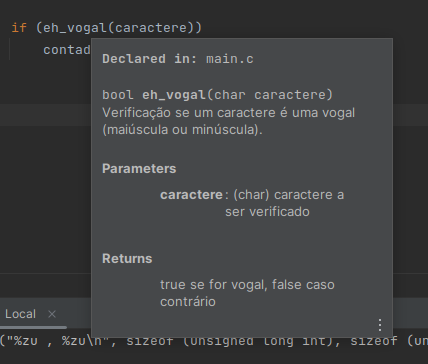
\includegraphics[width=0.6\linewidth,height=\textheight,keepaspectratio]{figuras/ide-popup.png}

}

\end{figure}%

\section{Criação de funções}\label{criauxe7uxe3o-de-funuxe7uxf5es}

Quando uma função é escrita em um programa, é importante que se tenha
clareza do seu objetivo. A função deve, em consequência, ater-se somente
a ele e não realizar outra tarefa qualquer. Por exemplo, se uma função é
escrita para converter graus Celsius para Fahrenheit, é somente a
conversão que deve ser feita; a função não deve ler nada nem escrever
nada.

Segue um exemplo dessa função.

\begin{Shaded}
\begin{Highlighting}[]
\CommentTok{/*!}
\CommentTok{ * Retorna a temperatura em Fahenheit dado seu valor em graus Celsius}
\CommentTok{ * }\AnnotationTok{@param}\CommentTok{ }\CommentVarTok{celsius:}\CommentTok{ a temperatura Celsius}
\CommentTok{ * }\AnnotationTok{@return}\CommentTok{ a temperatura em Fahrenheit}
\CommentTok{ */}
\DataTypeTok{double}\NormalTok{ celsius\_para\_fahrenheit}\OperatorTok{(}\DataTypeTok{double}\NormalTok{ celsius}\OperatorTok{)} \OperatorTok{\{}
    \ControlFlowTok{return} \FloatTok{1.8} \OperatorTok{*}\NormalTok{ celsius }\OperatorTok{+} \DecValTok{32}\OperatorTok{;}
\OperatorTok{\}}
\end{Highlighting}
\end{Shaded}

Todos os dados necessários devem ser passados como parâmetros e o
resultado retornado pela função.

Não se está dizendo aqui que função não podem nem ler nem escrever. Se
uma função tenha como objetivo ler um valor digitado pelo usuário, é
isso que ela tem que fazer. O programa exemplo seguinte inclui uma
função de interface para ler um valor inteiro digitado pelo usuário,
verificando erros e garantindo que um valor válido seja entrado.

\begin{Shaded}
\begin{Highlighting}[]
\CommentTok{/*}
\CommentTok{Leitura da idade de uma pessoa e escrita desse valor na tela}
\CommentTok{Requer: digitação de uma idade}
\CommentTok{Assegura: apresentação da idade na tela}
\CommentTok{*/}
\PreprocessorTok{\#include }\ImportTok{\textless{}stdio.h\textgreater{}}

\DataTypeTok{int}\NormalTok{ leia\_inteiro}\OperatorTok{(}\DataTypeTok{char} \OperatorTok{*}\NormalTok{mensagem}\OperatorTok{);}

\DataTypeTok{int}\NormalTok{ main}\OperatorTok{(}\DataTypeTok{void}\OperatorTok{)} \OperatorTok{\{}
    \DataTypeTok{int}\NormalTok{ idade }\OperatorTok{=}\NormalTok{ leia\_inteiro}\OperatorTok{(}\StringTok{"Digite sua idade: "}\OperatorTok{);}
\NormalTok{    printf}\OperatorTok{(}\StringTok{"Você tem }\SpecialCharTok{\%d}\StringTok{ anos de idade.}\SpecialCharTok{\textbackslash{}n}\StringTok{"}\OperatorTok{,}\NormalTok{ idade}\OperatorTok{);}

    \ControlFlowTok{return} \DecValTok{0}\OperatorTok{;}
\OperatorTok{\}}

\CommentTok{/*!}
\CommentTok{ * Retorna um valor inteiro válido digitado pelo usuário.}
\CommentTok{ * A leitura é repetida caso o valor digitado não corresponda a}
\CommentTok{ * um inteiro válido, sendo uma mensagem de aviso apresentada. Qualquer}
\CommentTok{ * texto depois do inteiro é descartado.}
\CommentTok{ * }\AnnotationTok{@param}\CommentTok{ }\CommentVarTok{mensagem:}\CommentTok{ mensagem solicitando a leitura}
\CommentTok{ * }\AnnotationTok{@return}\CommentTok{ um valor inteiro lido}
\CommentTok{ */}
\DataTypeTok{int}\NormalTok{ leia\_inteiro}\OperatorTok{(}\DataTypeTok{char} \OperatorTok{*}\NormalTok{mensagem}\OperatorTok{)} \OperatorTok{\{}
\NormalTok{    printf}\OperatorTok{(}\StringTok{"}\SpecialCharTok{\%s}\StringTok{"}\OperatorTok{,}\NormalTok{ mensagem}\OperatorTok{);}
    \DataTypeTok{int}\NormalTok{ valor\_lido}\OperatorTok{,}\NormalTok{ quantidade\_itens\_lidos}\OperatorTok{;}
    \ControlFlowTok{do} \OperatorTok{\{}
        \DataTypeTok{char}\NormalTok{ entrada}\OperatorTok{[}\DecValTok{160}\OperatorTok{];}
\NormalTok{        fgets}\OperatorTok{(}\NormalTok{entrada}\OperatorTok{,} \KeywordTok{sizeof}\NormalTok{ entrada}\OperatorTok{,}\NormalTok{ stdin}\OperatorTok{);}
\NormalTok{        quantidade\_itens\_lidos }\OperatorTok{=}\NormalTok{ sscanf}\OperatorTok{(}\NormalTok{entrada}\OperatorTok{,} \StringTok{"}\SpecialCharTok{\%d}\StringTok{"}\OperatorTok{,} \OperatorTok{\&}\NormalTok{valor\_lido}\OperatorTok{);}
        \ControlFlowTok{if} \OperatorTok{(}\NormalTok{quantidade\_itens\_lidos }\OperatorTok{!=} \DecValTok{1}\OperatorTok{)}
\NormalTok{            printf}\OperatorTok{(}\StringTok{"\textgreater{} Valor inválido. Esperado um inteiro.}\SpecialCharTok{\textbackslash{}n}\StringTok{"}
                   \StringTok{"}\SpecialCharTok{\%s}\StringTok{"}\OperatorTok{,}\NormalTok{ mensagem}\OperatorTok{);}
    \OperatorTok{\}} \ControlFlowTok{while} \OperatorTok{(}\NormalTok{quantidade\_itens\_lidos }\OperatorTok{!=} \DecValTok{1}\OperatorTok{);}

    \ControlFlowTok{return}\NormalTok{ valor\_lido}\OperatorTok{;}
\OperatorTok{\}}
\end{Highlighting}
\end{Shaded}

\begin{Shaded}
\begin{Highlighting}[]
\NormalTok{Digite sua idade: }\KeywordTok{abc}
\NormalTok{\textgreater{} Valor inválido. Esperado um inteiro.}
\NormalTok{Digite sua idade: }\KeywordTok{*}
\NormalTok{\textgreater{} Valor inválido. Esperado um inteiro.}
\NormalTok{Digite sua idade: }\KeywordTok{\#10}
\NormalTok{\textgreater{} Valor inválido. Esperado um inteiro.}
\NormalTok{Digite sua idade: }\KeywordTok{25}
\NormalTok{Você tem 25 anos de idade.}
\end{Highlighting}
\end{Shaded}

Há que se notar que a função deve ler e retornar um valor inteiro e
digitações erradas são detectadas e contornadas. Para ser uma função
genérica, ela lê inteiros e não idades (tanto que valores negativos
seriam aceitos nesse caso). Essa função pode ser usada em qualquer outro
programa para a leitura de um inteiro e ela não atende exclusivamente o
problema do programa em questão.

Caso fosse interessante garantir que o valor fosse maior que zero, outra
função poderia ser escrita para ler valores apenas em \(\mathbb{N}\).
Segue um exemplo de implementação de uma função que atende a esses
requisitos, a qual aproveita a já escrita \texttt{leia\_inteiro}, apenas
repassando a mensagem para o usuário. No programa anterior, bastaria
\texttt{main} executar \texttt{leia\_natural} no lugar de
\texttt{leia\_inteiro}.

\begin{Shaded}
\begin{Highlighting}[]
\CommentTok{/*!}
\CommentTok{ * Retorna um valor inteiro natural digitado pelo usuário.}
\CommentTok{ * A leitura é repetida para valores inválidos e o restante da linha}
\CommentTok{ * depois do inteiro é ignorado}
\CommentTok{ * }\AnnotationTok{@param}\CommentTok{ }\CommentVarTok{mensagem:}\CommentTok{ mensagem solicitando a leitura}
\CommentTok{ * }\AnnotationTok{@return}\CommentTok{ valor inteiro lido, maior ou igual a zero}
\CommentTok{ */}
\DataTypeTok{int}\NormalTok{ leia\_natural}\OperatorTok{(}\DataTypeTok{char} \OperatorTok{*}\NormalTok{mensagem}\OperatorTok{)} \OperatorTok{\{}
    \DataTypeTok{int}\NormalTok{ valor\_lido}\OperatorTok{;}
    \ControlFlowTok{do} \OperatorTok{\{}
\NormalTok{        valor\_lido }\OperatorTok{=}\NormalTok{ leia\_inteiro}\OperatorTok{(}\NormalTok{mensagem}\OperatorTok{);}
        \ControlFlowTok{if} \OperatorTok{(}\NormalTok{valor\_lido }\OperatorTok{\textless{}} \DecValTok{0}\OperatorTok{)}
\NormalTok{            printf}\OperatorTok{(}\StringTok{"Valor inválido. Esperado maior ou igual a zero.}\SpecialCharTok{\textbackslash{}n}\StringTok{"}\OperatorTok{);}
    \OperatorTok{\}} \ControlFlowTok{while} \OperatorTok{(}\NormalTok{valor\_lido }\OperatorTok{\textless{}} \DecValTok{0}\OperatorTok{);}
    \ControlFlowTok{return}\NormalTok{ valor\_lido}\OperatorTok{;}
\OperatorTok{\}}
\end{Highlighting}
\end{Shaded}

\section{Escolha dos tipos de retorno e dos
parâmetros}\label{escolha-dos-tipos-de-retorno-e-dos-paruxe2metros}

Os tipos dos parâmetros devem satisfazer as necessidades das funções.
Por exemplo, na conversão de graus Celsius para Fahrenheit é esperado
que a temperatura em Celsius seja \texttt{double}, assim como o valor
retornado em Fahrenheit.

\begin{Shaded}
\begin{Highlighting}[]
\DataTypeTok{double}\NormalTok{ celsius\_para\_fahrenheit}\OperatorTok{(}\DataTypeTok{double}\NormalTok{ celsius}\OperatorTok{);}
\end{Highlighting}
\end{Shaded}

Para uma função do cálculo do fatorial de um número, entretanto, as
escolhas podem não ser tão elementares. Uma primeira tentativa seria,
por exemplo, ter a função com o seguinte protótipo.

\begin{Shaded}
\begin{Highlighting}[]
\DataTypeTok{int}\NormalTok{ fatorial}\OperatorTok{(}\DataTypeTok{int}\NormalTok{ n}\OperatorTok{);}
\end{Highlighting}
\end{Shaded}

Um primeiro ponto é que, nos sistemas atuais, um \texttt{int} ocupa
geralmente quatro bytes e permite valores de -2.147.483.648 a
2.147.483.647. Metade dos valores representados são negativos e o
resultado do fatorial nunca será negativo. Assim, pode-se optar pela
prototipagem seguinte.

\begin{Shaded}
\begin{Highlighting}[]
\DataTypeTok{unsigned} \DataTypeTok{int}\NormalTok{ fatorial}\OperatorTok{(}\DataTypeTok{int}\NormalTok{ n}\OperatorTok{);}
\end{Highlighting}
\end{Shaded}

Nessa nova versão, ainda considerando os tamanhos típicos para inteiros,
os valores de retorno podem ser de zero a 4.294.967.295. Esse intervalo
comportaria valores até 12\(!\) (479.001.600), pois 13\(!\)
(6.227.020.800) já extrapolaria.

A versão seguinte expande o tipo de retorno para
\texttt{unsigned\ long\ int}, o qual usa oito bytes na versão do
\texttt{gcc} usada nos programas. Desse modo, a gama de possíveis
resultados vai para 18.446.744.073.709.551.615, o que comportaria até
20\(!\)\footnote{Embora 20\(!\) não pareça muito, vale lembrar seu valor
  é 2.432.902.008.176.640.000, ou seja, aproximadamente
  2,4~\(\times\)~10\textsuperscript{18}.}.

\begin{Shaded}
\begin{Highlighting}[]
\DataTypeTok{unsigned} \DataTypeTok{long} \DataTypeTok{int}\NormalTok{ fatorial}\OperatorTok{(}\DataTypeTok{int}\NormalTok{ n}\OperatorTok{);}
\end{Highlighting}
\end{Shaded}

O mesmo raciocínio se aplicaria ao parâmetro \texttt{n}. Para \(n!\),
sempre se tem \(n \geq 0\), e, assim, a função poderia ter como
protótipo final o formato que segue.

\begin{Shaded}
\begin{Highlighting}[]
\DataTypeTok{unsigned} \DataTypeTok{long} \DataTypeTok{int}\NormalTok{ fatorial}\OperatorTok{(}\DataTypeTok{unsigned} \DataTypeTok{int}\NormalTok{ n}\OperatorTok{);}
\end{Highlighting}
\end{Shaded}

Sua implementação seria como se segue.

\begin{Shaded}
\begin{Highlighting}[]
\CommentTok{/*!}
\CommentTok{ * Retorna, para um dado n, o valor de n!}
\CommentTok{ * }\AnnotationTok{@param}\CommentTok{ }\CommentVarTok{n:}\CommentTok{ valor para o qual seu fatorial é calculado, n \textgreater{}= 0}
\CommentTok{ * }\AnnotationTok{@return}\CommentTok{ n!}
\CommentTok{ */}
\DataTypeTok{unsigned} \DataTypeTok{long} \DataTypeTok{int}\NormalTok{ fatorial}\OperatorTok{(}\DataTypeTok{unsigned} \DataTypeTok{int}\NormalTok{ n}\OperatorTok{)} \OperatorTok{\{}
    \DataTypeTok{unsigned} \DataTypeTok{long} \DataTypeTok{int}\NormalTok{ multiplicador }\OperatorTok{=} \DecValTok{1}\OperatorTok{;}
    \ControlFlowTok{for} \OperatorTok{(}\DataTypeTok{unsigned} \DataTypeTok{int}\NormalTok{ i }\OperatorTok{=} \DecValTok{2}\OperatorTok{;}\NormalTok{ i }\OperatorTok{\textless{}=}\NormalTok{ n}\OperatorTok{;}\NormalTok{ i}\OperatorTok{++)}
\NormalTok{        multiplicador }\OperatorTok{*=}\NormalTok{ i}\OperatorTok{;}

    \ControlFlowTok{return}\NormalTok{ multiplicador}\OperatorTok{;}
\OperatorTok{\}}
\end{Highlighting}
\end{Shaded}

A vantagem na escolha dos tipos é que, até certo limite, o compilador
consegue verificar consistência nos valores passados para a função. Por
exemplo, se houver uma variável \texttt{i} do tipo \texttt{int} (que
possui valores negativos), o compilador pode avisar (não é erro) que
pode haver algum problema. A mensagem de compilação seguinte mostra que
pode haver um problema de conversão caso os valores sejam negativos e o
resultado, portanto, pode não ser confiável.

\begin{Shaded}
\begin{Highlighting}[]
\NormalTok{main.c:18:31: warning: conversion to ‘unsigned int’ from ‘int’ may change}
\NormalTok{the sign of the result [{-}Wsign{-}conversion]}
\NormalTok{   18 |     printf("\%lu.\textbackslash{}n", fatorial(i));}
\NormalTok{      |                               \^{}}
\end{Highlighting}
\end{Shaded}

A boa escolha dos tipos sempre proporciona uma camada adicional de
controle na escrita de programas.

\chapter{Regras de escopo com a
modularização}\label{sec-regras-de-escopo-com-modularizacao}

Este capítulo estende os conceitos de escopo de validade das declarações
na linguagem C. A Seção~\ref{sec-declaracoes-e-validade} abordou as
declarações de variáveis internas (locais) a \texttt{main}, enquanto na
Seção~\ref{sec-escopo-da-declaracao-de-funcoes}. Esses assuntos são
revisitados e integrados.

Além de variáveis e funções, há outros elementos em C que podem ser
declarados. Esses não serão cobertos diretamente neste texto e, em
grande parte, a discussão exposta aqui também se aplica a eles.

\section{\texorpdfstring{Local \(\times\)
global}{Local \textbackslash times global}}\label{local-times-global}

Um código fonte escrito em C contém declarações, sejam de funções ou de
variáveis. Esse código fonte está contido em um arquivo texto,
usualmente com extensão \texttt{.c}.

Qualquer função declarada no arquivo tem escopo global, o que quer dizer
que sua validade vai desde a linha em que ocorre a declaração até a
última linha do arquivo. Em outras palavras, essa função é conhecida e
pode ser usada dentro de seu escopo de declaração. Essa regra aplica-se
tanto à declaração simples, na forma de protótipo de função, quanto às
implementações sem o protótipo
(Seção~\ref{sec-escopo-da-declaracao-de-funcoes}).

Outra forma de olhar para essa questão é considerar global qualquer
declaração feita fora de uma função.

Como existe o conceito de ``fora de uma função'', também há o de
``dentro de uma função''. Assim, variáveis declaradas no corpo da
implementação de uma função estão dentro da função e são chamadas de
declarações locais. O termo se aplica também aos parâmetros formais da
função.

\subsection{Validade das declarações globais e
locais}\label{validade-das-declarauxe7uxf5es-globais-e-locais}

Para exemplificar tanto declarações globais quanto locais quanto suas
validades, segue um programa para simplificação de números racionais, o
qual emprega uma função para o cálculo do máximo divisor comum (MDC)
entre dois números inteiros e outra para o cálculo do valor absoluto
(módulo, \(\lvert n\rvert\)) de um inteiro. O objetivo do programa é
simplificar um número racional, lembrando que \(q \in \mathbb{Q}\) é um
valor expresso na forma \(a/b\), sendo \(a \in \mathbb{Z}\) com
\(b \in \mathbb{Z}^*\).

A lógica de modificação do número racional é apresentada no
Algoritmo~\ref{alg-simplificacao-padronizacao-racionais}.

\begin{algorithm}[H]
\caption{\label{alg-simplificacao-padronizacao-racionais}Leitura e
apresentação de números racionais.}
\begingroup%

%| title: Leitura e apresentação de números racionais.
%| label: #alg-simplificacao-padronizacao-racionais

\begin{algorithmic}
    \Description Leitura de um valor racional na forma $\frac{a}{b}$ e sua apresentação, padronizando para mostrar o sinal (se negativo) e sua forma fracionária simplificada
    \Require número racional $\frac{a}{b}$
    \Ensure apresentação do racional em forma padronizada
    \Statex{}
    \Statep{Obtenha o racional $r = \frac{a}{b}$}
    \Statep{Determine o valor do sinal de $r$}[$1$ ou $-1$]
    \Statep{Calcule o MDC entre $a$ e $b$, guardando em \Id{fator}}
    \Statep{Calcule $a'$ e $b'$ com, respectivamente, $\lvert a\rvert$ e $\lvert b\rvert$}
    \Statep{Modifique o valor de $a'$ para ter o sinal de $r$ e o valor $\frac{a'}{\Id{fator}}$}[simplifica o numerador]
    \Statep{Modifique o valor de $b'$ para $\frac{b'}{\Id{fator}}$}[simplifica o denominador]
    \Statep{Apresente $r' = \frac{a'}{b'}$}[o sinal já está presente em $a'$]
\end{algorithmic}

\endgroup
\end{algorithm}

A codificação em C é apresentada na sequência.

\begin{Shaded}
\begin{Highlighting}[numbers=left,,]
\CommentTok{/*}
\CommentTok{ * Leitura e escrita de um número racional na forma de fração}
\CommentTok{ * Requer: a digitação de um valor a/b, a,b inteiros, b != 0}
\CommentTok{ * Assegura: apresentação do mesmo valor em forma simplificada e padronizada}
\CommentTok{ */}
\PreprocessorTok{\#include }\ImportTok{\textless{}stdio.h\textgreater{}}

\CommentTok{/*!}
\CommentTok{ * Retorna o MDC de dois inteiros quaisquer (máximo divisor comum).}
\CommentTok{ * }\AnnotationTok{@param}\CommentTok{ }\CommentVarTok{n1:}\CommentTok{ primeiro valor}
\CommentTok{ * }\AnnotationTok{@param}\CommentTok{ }\CommentVarTok{n2:}\CommentTok{ segundo valor}
\CommentTok{ * }\AnnotationTok{@return}\CommentTok{ MDC(n1, n2)}
\CommentTok{ */}
\DataTypeTok{unsigned} \DataTypeTok{int}\NormalTok{ mdc}\OperatorTok{(}\DataTypeTok{int}\NormalTok{ n1}\OperatorTok{,} \DataTypeTok{int}\NormalTok{ n2}\OperatorTok{);}

\CommentTok{/*!}
\CommentTok{ * Retorna o valor absoluto de um inteiro}
\CommentTok{ * }\AnnotationTok{@param}\CommentTok{ }\CommentVarTok{n:}\CommentTok{ valor inteiro}
\CommentTok{ * }\AnnotationTok{@return}\CommentTok{ o valor absoluto do número, |n|}
\CommentTok{ */}
\DataTypeTok{int}\NormalTok{ valor\_absoluto}\OperatorTok{(}\DataTypeTok{int}\NormalTok{ n}\OperatorTok{);}

\CommentTok{/*}
\CommentTok{ * Main}
\CommentTok{ */}
\DataTypeTok{int}\NormalTok{ main}\OperatorTok{()} \OperatorTok{\{}
    \CommentTok{// Leitura}
\NormalTok{    printf}\OperatorTok{(}\StringTok{"Digite um número racional a/b (a e b inteiros e b não nulo): "}\OperatorTok{);}
    \DataTypeTok{char}\NormalTok{ entrada}\OperatorTok{[}\DecValTok{160}\OperatorTok{];}
\NormalTok{    fgets}\OperatorTok{(}\NormalTok{entrada}\OperatorTok{,} \KeywordTok{sizeof}\NormalTok{ entrada}\OperatorTok{,}\NormalTok{ stdin}\OperatorTok{);}
    \DataTypeTok{int}\NormalTok{ numerador}\OperatorTok{,}\NormalTok{ denominador}\OperatorTok{;}
\NormalTok{    sscanf}\OperatorTok{(}\NormalTok{entrada}\OperatorTok{,} \StringTok{"}\SpecialCharTok{\%d}\StringTok{/}\SpecialCharTok{\%d}\StringTok{"}\OperatorTok{,} \OperatorTok{\&}\NormalTok{numerador}\OperatorTok{,} \OperatorTok{\&}\NormalTok{denominador}\OperatorTok{);}

    \CommentTok{// Simplificação da fração e colocação do sinal no numerador}
    \ControlFlowTok{if} \OperatorTok{(}\NormalTok{numerador }\OperatorTok{==} \DecValTok{0}\OperatorTok{)}
\NormalTok{        denominador }\OperatorTok{=} \DecValTok{1}\OperatorTok{;}  \CommentTok{// o valor zero é padronizado para 0/1}
    \ControlFlowTok{else} \OperatorTok{\{}
        \DataTypeTok{int}\NormalTok{ fator\_divisao }\OperatorTok{=}\NormalTok{ mdc}\OperatorTok{(}\NormalTok{numerador}\OperatorTok{,}\NormalTok{ denominador}\OperatorTok{);}
        \DataTypeTok{int}\NormalTok{ sinal\_da\_fracao }\OperatorTok{=} \OperatorTok{((}\DataTypeTok{double}\OperatorTok{)}\NormalTok{numerador }\OperatorTok{/}\NormalTok{ denominador }\OperatorTok{\textgreater{}=} \DecValTok{0}\OperatorTok{)} \OperatorTok{?} \DecValTok{1} \OperatorTok{:} \OperatorTok{{-}}\DecValTok{1}\OperatorTok{;}
\NormalTok{        numerador }\OperatorTok{=}\NormalTok{ valor\_absoluto}\OperatorTok{(}\NormalTok{numerador}\OperatorTok{);}
\NormalTok{        denominador }\OperatorTok{=}\NormalTok{ valor\_absoluto}\OperatorTok{(}\NormalTok{denominador}\OperatorTok{);}
\NormalTok{        numerador }\OperatorTok{/=}\NormalTok{ sinal\_da\_fracao }\OperatorTok{*}\NormalTok{ fator\_divisao}\OperatorTok{;}
\NormalTok{        denominador }\OperatorTok{/=}\NormalTok{ fator\_divisao}\OperatorTok{;}
    \OperatorTok{\}}

    \CommentTok{// Resultado}
\NormalTok{    printf}\OperatorTok{(}\StringTok{"O racional digitado foi: }\SpecialCharTok{\%d}\StringTok{/}\SpecialCharTok{\%d}\StringTok{.}\SpecialCharTok{\textbackslash{}n}\StringTok{"}\OperatorTok{,}\NormalTok{ numerador}\OperatorTok{,}\NormalTok{ denominador}\OperatorTok{);}

    \ControlFlowTok{return} \DecValTok{0}\OperatorTok{;}
\OperatorTok{\}}

\CommentTok{// Máximo divisor comum: MDC(n1, n2)}
\DataTypeTok{unsigned} \DataTypeTok{int}\NormalTok{ mdc}\OperatorTok{(}\DataTypeTok{int}\NormalTok{ n1}\OperatorTok{,} \DataTypeTok{int}\NormalTok{ n2}\OperatorTok{)} \OperatorTok{\{}
    \CommentTok{// Converte n1 e n2 para valores positivos}
\NormalTok{    n1 }\OperatorTok{=}\NormalTok{ valor\_absoluto}\OperatorTok{(}\NormalTok{n1}\OperatorTok{);}
\NormalTok{    n2 }\OperatorTok{=}\NormalTok{ valor\_absoluto}\OperatorTok{(}\NormalTok{n2}\OperatorTok{);}

    \CommentTok{// Resolução pelo método de Euclides}
    \DataTypeTok{int}\NormalTok{ resto}\OperatorTok{;}
    \ControlFlowTok{do} \OperatorTok{\{}
\NormalTok{        resto }\OperatorTok{=}\NormalTok{ n1 }\OperatorTok{\%}\NormalTok{ n2}\OperatorTok{;}
\NormalTok{        n1 }\OperatorTok{=}\NormalTok{ n2}\OperatorTok{;}
\NormalTok{        n2 }\OperatorTok{=}\NormalTok{ resto}\OperatorTok{;}
    \OperatorTok{\}} \ControlFlowTok{while} \OperatorTok{(}\NormalTok{resto }\OperatorTok{!=} \DecValTok{0}\OperatorTok{);}

    \ControlFlowTok{return}\NormalTok{ n1}\OperatorTok{;}  \CommentTok{// Contém o MDC no final}
\OperatorTok{\}}

\CommentTok{// Valor absoluto de um inteiro}
\DataTypeTok{int}\NormalTok{ valor\_absoluto}\OperatorTok{(}\DataTypeTok{int}\NormalTok{ n}\OperatorTok{)} \OperatorTok{\{}
    \ControlFlowTok{return} \OperatorTok{(}\NormalTok{n }\OperatorTok{\textgreater{}=} \DecValTok{0}\OperatorTok{)} \OperatorTok{?}\NormalTok{ n }\OperatorTok{:} \OperatorTok{{-}}\NormalTok{n}\OperatorTok{;}
\OperatorTok{\}}
\end{Highlighting}
\end{Shaded}

\begin{Shaded}
\begin{Highlighting}[]
\NormalTok{Digite um número racional a/b (a e b inteiros e b não nulo): }\KeywordTok{{-}3553/{-}627}
\NormalTok{O racional digitado foi: 17/3.}
\end{Highlighting}
\end{Shaded}

Para esse programa, há declarações tanto de variáveis quanto de funções.
A Tabela~\ref{tbl-validade-declaracoes-racionais} apresenta as
declarações de interesse no programa e destaca o escopo e validade
(linhas do código) de cada uma.

\begin{longtable}[]{@{}
  >{\raggedright\arraybackslash}p{(\linewidth - 8\tabcolsep) * \real{0.4000}}
  >{\centering\arraybackslash}p{(\linewidth - 8\tabcolsep) * \real{0.1286}}
  >{\centering\arraybackslash}p{(\linewidth - 8\tabcolsep) * \real{0.3429}}
  >{\centering\arraybackslash}p{(\linewidth - 8\tabcolsep) * \real{0.0857}}
  >{\centering\arraybackslash}p{(\linewidth - 8\tabcolsep) * \real{0.0429}}@{}}
\caption{Declarações relevantes feitas no programa de apresentação de
números racionais, seu tipo, escopo e linhas em que são
válidas.}\label{tbl-validade-declaracoes-racionais}\tabularnewline
\toprule\noalign{}
\begin{minipage}[b]{\linewidth}\raggedright
Declaração
\end{minipage} & \begin{minipage}[b]{\linewidth}\centering
Tipo
\end{minipage} & \begin{minipage}[b]{\linewidth}\centering
Escopo
\end{minipage} & \begin{minipage}[b]{\linewidth}\centering
Início
\end{minipage} & \begin{minipage}[b]{\linewidth}\centering
Fim
\end{minipage} \\
\midrule\noalign{}
\endfirsthead
\toprule\noalign{}
\begin{minipage}[b]{\linewidth}\raggedright
Declaração
\end{minipage} & \begin{minipage}[b]{\linewidth}\centering
Tipo
\end{minipage} & \begin{minipage}[b]{\linewidth}\centering
Escopo
\end{minipage} & \begin{minipage}[b]{\linewidth}\centering
Início
\end{minipage} & \begin{minipage}[b]{\linewidth}\centering
Fim
\end{minipage} \\
\midrule\noalign{}
\endhead
\bottomrule\noalign{}
\endlastfoot
\texttt{mdc} & função & global & 14 & 68 \\
\texttt{valor\_absoluto} & função & global & 21 & 68 \\
\texttt{entrada} & variável & local (\texttt{main}) & 29 & 46 \\
\texttt{numerador}, \texttt{denominador} & variável & local
(\texttt{main}) & 31 & 46 \\
\texttt{fator\_divisao} & variável & local (\texttt{main}) & 35 & 46 \\
\texttt{sinal\_da\_fracao} & variável & local (\texttt{main}) & 36 &
46 \\
\texttt{n1}, \texttt{n2} & parâmetro & local (\texttt{mdc}) & 49 & 63 \\
\texttt{resto} & variável & local (\texttt{mdc}) & 55 & 63 \\
\texttt{n} & parâmetro & local (\texttt{valor\_absoluto}) & 66 & 68 \\
\end{longtable}

\begin{tcolorbox}[enhanced jigsaw, arc=.35mm, bottomtitle=1mm, colbacktitle=quarto-callout-tip-color!10!white, title=\textcolor{quarto-callout-tip-color}{\faLightbulb}\hspace{0.5em}{Curiosidade}, toprule=.15mm, left=2mm, opacityback=0, colback=white, colframe=quarto-callout-tip-color-frame, opacitybacktitle=0.6, bottomrule=.15mm, leftrule=.75mm, toptitle=1mm, coltitle=black, titlerule=0mm, rightrule=.15mm, breakable]

É interessante apontar que \texttt{n1} e \texttt{n2} na linha 14, assim
como \texttt{n} na linha 21 do programa apresentado não possuem
validade, pois o protótipo de uma função é apenas sua declaração e, como
tal, seus parâmetros não são realmente criados, mas apenas informados ao
compilador.

Na prática, a linha 14 do código do programa poderia ser escrita como
segue, mas com o prejuízo de reduzir as informações de documentação do
programa ao não informar semanticamente a que cada parâmetro se refere.

\begin{Shaded}
\begin{Highlighting}[]
\DataTypeTok{unsigned} \DataTypeTok{int}\NormalTok{ mdc}\OperatorTok{(}\DataTypeTok{int}\OperatorTok{,} \DataTypeTok{int}\OperatorTok{);}  \CommentTok{// o nome dos parâmetros é irrelevante, mas sua}
                             \CommentTok{// omissão prejudica a documentação e legibilidade}
\end{Highlighting}
\end{Shaded}

\end{tcolorbox}

\section{Reuso de identificadores}\label{reuso-de-identificadores}

Nos programa em C é possível usar um mesmo identificador desde que eles
suas declarações atendam escopos diferentes. Dessa forma, um
identificador \texttt{p} pode ser parâmetro para diversas funções
diferentes. Da mesma forma, uma variável local a uma função não conflita
com qualquer outra declaração. O compilador reclamará, assim, apenas de
duas declarações globais com mesmo identificador ou então o uso de um
mesmo nome em duplicidade no mesmo contexto local.

A seguir é apresentado um código fonte genérico, não realiza qualquer
processamento útil, O objetivo é indicar como identificadores iguais são
tratados.

\begin{Shaded}
\begin{Highlighting}[]
\CommentTok{/*}
\CommentTok{ * Programa exemplo de declarações}
\CommentTok{ */}
\PreprocessorTok{\#include }\ImportTok{\textless{}stdio.h\textgreater{}}

\DataTypeTok{int}\NormalTok{ f1}\OperatorTok{(}\DataTypeTok{int}\NormalTok{ a}\OperatorTok{,} \DataTypeTok{int}\NormalTok{ b}\OperatorTok{);}

\DataTypeTok{double}\NormalTok{ f2}\OperatorTok{(}\DataTypeTok{double}\NormalTok{ a}\OperatorTok{);}

\DataTypeTok{int}\NormalTok{ f3}\OperatorTok{(}\DataTypeTok{double}\NormalTok{ f1}\OperatorTok{,} \DataTypeTok{double}\NormalTok{ f2}\OperatorTok{);}

\DataTypeTok{int}\NormalTok{ main}\OperatorTok{(}\DataTypeTok{void}\OperatorTok{)} \OperatorTok{\{}
    \DataTypeTok{int}\NormalTok{ a}\OperatorTok{,}\NormalTok{ b}\OperatorTok{,}\NormalTok{ c}\OperatorTok{;}
    \DataTypeTok{double}\NormalTok{ d }\OperatorTok{=} \FloatTok{1.25}\OperatorTok{;}

\NormalTok{    a }\OperatorTok{=} \OperatorTok{(}\DataTypeTok{int}\OperatorTok{)}\NormalTok{f2}\OperatorTok{(}\NormalTok{d}\OperatorTok{);}
\NormalTok{    b }\OperatorTok{=}\NormalTok{ f3}\OperatorTok{(}\NormalTok{d}\OperatorTok{,} \FloatTok{0.5} \OperatorTok{*}\NormalTok{ a}\OperatorTok{);}
\NormalTok{    c }\OperatorTok{=}\NormalTok{ f1}\OperatorTok{(}\NormalTok{a}\OperatorTok{,}\NormalTok{ b}\OperatorTok{);}

\NormalTok{    printf}\OperatorTok{(}\StringTok{"}\SpecialCharTok{\%d}\StringTok{ }\SpecialCharTok{\%d}\StringTok{ }\SpecialCharTok{\%d}\StringTok{ }\SpecialCharTok{\%g\textbackslash{}n}\StringTok{"}\OperatorTok{,}\NormalTok{ a}\OperatorTok{,}\NormalTok{ b}\OperatorTok{,}\NormalTok{ c}\OperatorTok{,}\NormalTok{ d}\OperatorTok{);}

    \ControlFlowTok{return} \DecValTok{0}\OperatorTok{;}
\OperatorTok{\}}

\DataTypeTok{int}\NormalTok{ f1}\OperatorTok{(}\DataTypeTok{int}\NormalTok{ a}\OperatorTok{,} \DataTypeTok{int}\NormalTok{ b}\OperatorTok{)} \OperatorTok{\{}
    \DataTypeTok{int}\NormalTok{ n }\OperatorTok{=}\NormalTok{ f3}\OperatorTok{(}\NormalTok{a}\OperatorTok{,}\NormalTok{ b}\OperatorTok{);}
    \ControlFlowTok{return}\NormalTok{ a }\OperatorTok{+}\NormalTok{ b }\OperatorTok{+}\NormalTok{ n}\OperatorTok{;}
\OperatorTok{\}}

\DataTypeTok{double}\NormalTok{ f2}\OperatorTok{(}\DataTypeTok{double}\NormalTok{ a}\OperatorTok{)} \OperatorTok{\{}
    \DataTypeTok{int}\NormalTok{ n }\OperatorTok{=} \DecValTok{1}\OperatorTok{;}
    \DataTypeTok{double}\NormalTok{ b }\OperatorTok{=}\NormalTok{ f1}\OperatorTok{(}\NormalTok{a}\OperatorTok{,}\NormalTok{ n}\OperatorTok{);}
    \ControlFlowTok{return}\NormalTok{ b}\OperatorTok{;}
\OperatorTok{\}}

\DataTypeTok{int}\NormalTok{ f3}\OperatorTok{(}\DataTypeTok{double}\NormalTok{ f1}\OperatorTok{,} \DataTypeTok{double}\NormalTok{ f2}\OperatorTok{)} \OperatorTok{\{}
    \DataTypeTok{int}\NormalTok{ main }\OperatorTok{=} \OperatorTok{(}\DataTypeTok{int}\OperatorTok{)}\NormalTok{f1 }\OperatorTok{+} \OperatorTok{(}\DataTypeTok{int}\OperatorTok{)}\NormalTok{f2}\OperatorTok{;}
    \ControlFlowTok{return}\NormalTok{ main}\OperatorTok{;}
\OperatorTok{\}}
\end{Highlighting}
\end{Shaded}

\begin{Shaded}
\begin{Highlighting}[]
\NormalTok{4 3 14 1.25}
\end{Highlighting}
\end{Shaded}

Os pontos que requerem atenção neste programa são os seguintes:

\begin{itemize}
\tightlist
\item
  As funções \texttt{f1}, \texttt{f2} e \texttt{f3} têm validade em
  praticamente todo o programa;
\item
  Ambas as funções \texttt{f1} e \texttt{f2} possuem parâmetro com
  identificador \texttt{a}, mas eles são independentes pois estão em
  escopos diferentes;
\item
  A função principal \texttt{main} também possui variáveis locais
  \texttt{a} e \texttt{b}, também disjuntas dos parâmetros e outras
  declarações locais;
\item
  Tanto \texttt{f1} quanto \texttt{f2} possuem variáveis locais chamadas
  \texttt{n}, sendo elas completamente separadas dado seu escopo local
  diferente;
\item
  A função \texttt{f1} chama \texttt{f3}, que é conhecida dado o escopo
  global, sendo que o mesmo ocorre com a chamada de \texttt{f1} em
  \texttt{f2};
\item
  \texttt{f3} possui parâmetros \texttt{f1} e \texttt{f2}, cujos nomes
  se sobrepõem às funções globais \texttt{f1} e \texttt{f2},
  significando que, dentro de \texttt{f3}, essas funções não estão
  acessíveis pois são obscurecidas pelas declarações locais;
\item
  \texttt{f3} possui uma variável local \texttt{main}, que não conflita
  com a função global com mesmo nome.
\end{itemize}

Dessa forma, seguem algumas orientações gerais de escopo:

\begin{itemize}
\tightlist
\item
  Declarações globais valem em todo o código fonte a partir de sua
  declaração;
\item
  Parâmetros e declarações em funções são locais, têm apenas validade no
  escopo da função e são independentes de qualquer outra declaração com
  mesmo nome em escopo maior;
\item
  Declarações locais podem se sobrepor e ocultar declarações globais;
\item
  Blocos de comandos podem ter declarações cujo escopo é o próprio bloco
  apenas (Seção~\ref{sec-declaracoes-e-validade}).
\end{itemize}

\section{Variáveis globais}\label{variuxe1veis-globais}

Assim como funções, também variáveis podem ser globais. Uma variável
declarada fora do escopo de qualquer função é uma variável global e,
como tal, tem sua validade definida e conhecida desde a linha em que é
declarada até o final do arquivo.

Variáveis declaradas como globais possuem duas diferenças importantes em
relação às locais, sejam variáveis ou parâmetros de funções:

\begin{itemize}
\tightlist
\item
  Local e momento de criação;
\item
  Iniciação automática.
\end{itemize}

A primeira diferença, portanto, é que as variáveis globais são criadas
juntamente com a execução do programa e possuem um espaço de memória
específico para elas. As variáveis locais e os parâmetros são criados
apenas no momento em que a função é chamada e, dependendo de quando isso
ocorre, podem ser criadas em diferentes locais da memória dependendo da
chamada.

Variáveis globais são consideradas estáticas enquanto as locais são
criadas dinamicamente em função do momento em que as funções são
chamadas

O segundo ponto é que as variáveis locais nunca possuem lixo, ou seja,
são sempre iniciadas com valores nulos. Assim, se uma variável global
\texttt{int\ i} é criada sem atribuição, seu valor será necessariamente
zero. Caso exista um \texttt{double\ d} global, o valor de \texttt{d}
será 0,0, exceto se houver outro valor inicial. De forma similar, se uma
cadeia de caracteres for criada em escopo global com
\texttt{char\ s{[}100{]}}, ela terá comprimento zero, pois todas suas
posições terão \texttt{\textbackslash{}0}.

\subsection{Declaração de variáveis
globais}\label{declarauxe7uxe3o-de-variuxe1veis-globais}

Para que uma variável seja global, basta que sua declaração seja feita
fora de uma função. Segue um exemplo simples em que foi criado um
contador global para monitorar o número de vezes que uma

\begin{Shaded}
\begin{Highlighting}[]
\CommentTok{/*}
\CommentTok{ * Programa exemplo com variável global}
\CommentTok{ * O código cria duas funções, volta\_igual e volta\_negativo, mantendo}
\CommentTok{ *      controle sobre o número de vezes que elas são chamadas}
\CommentTok{ * Assegura: apresentações diversas do uso da função e do número de vezes}
\CommentTok{ *      em que foram chamadas}
\CommentTok{ */}
\PreprocessorTok{\#include }\ImportTok{\textless{}stdio.h\textgreater{}}

\CommentTok{//! Contador para uso global}
\DataTypeTok{int}\NormalTok{ numero\_chamadas}\OperatorTok{;}

\CommentTok{/*!}
\CommentTok{ * Retorna igual ao que foi passado}
\CommentTok{ * }\AnnotationTok{@param}\CommentTok{ }\CommentVarTok{n}
\CommentTok{ * }\AnnotationTok{@return}\CommentTok{ n}
\CommentTok{ */}
\DataTypeTok{int}\NormalTok{ volta\_igual}\OperatorTok{(}\DataTypeTok{int}\NormalTok{ n}\OperatorTok{);}

\CommentTok{/*!}
\CommentTok{ * Retorna o oposto do que foi passado}
\CommentTok{ * }\AnnotationTok{@param}\CommentTok{ }\CommentVarTok{n}
\CommentTok{ * }\AnnotationTok{@return}\CommentTok{ {-}n}
\CommentTok{ */}
\DataTypeTok{int}\NormalTok{ volta\_negativo}\OperatorTok{(}\DataTypeTok{int}\NormalTok{ n}\OperatorTok{);}

\CommentTok{/*}
\CommentTok{ * Main}
\CommentTok{ */}
\DataTypeTok{int}\NormalTok{ main}\OperatorTok{(}\DataTypeTok{void}\OperatorTok{)} \OperatorTok{\{}
\NormalTok{    printf}\OperatorTok{(}\StringTok{"}\SpecialCharTok{\%d}\StringTok{ = }\SpecialCharTok{\%d}\StringTok{.}\SpecialCharTok{\textbackslash{}n}\StringTok{"}\OperatorTok{,} \DecValTok{10}\OperatorTok{,}\NormalTok{ volta\_igual}\OperatorTok{(}\DecValTok{10}\OperatorTok{));}
\NormalTok{    printf}\OperatorTok{(}\StringTok{"}\SpecialCharTok{\%d}\StringTok{ = {-}1 * }\SpecialCharTok{\%d}\StringTok{.}\SpecialCharTok{\textbackslash{}n\textbackslash{}n}\StringTok{"}\OperatorTok{,} \OperatorTok{{-}}\DecValTok{10}\OperatorTok{,}\NormalTok{ volta\_negativo}\OperatorTok{({-}}\DecValTok{10}\OperatorTok{));}
    \ControlFlowTok{for} \OperatorTok{(}\DataTypeTok{int}\NormalTok{ n }\OperatorTok{=} \OperatorTok{{-}}\DecValTok{5}\OperatorTok{;}\NormalTok{ n }\OperatorTok{\textless{}=} \DecValTok{5}\OperatorTok{;}\NormalTok{ n}\OperatorTok{++)}
\NormalTok{        printf}\OperatorTok{(}\StringTok{"}\SpecialCharTok{\%d}\StringTok{ = }\SpecialCharTok{\%d}\StringTok{ = {-}1 * }\SpecialCharTok{\%d}\StringTok{.}\SpecialCharTok{\textbackslash{}n}\StringTok{"}\OperatorTok{,}\NormalTok{ n}\OperatorTok{,}\NormalTok{ volta\_igual}\OperatorTok{(}\NormalTok{n}\OperatorTok{),}\NormalTok{ volta\_negativo}\OperatorTok{(}\NormalTok{n}\OperatorTok{));}

\NormalTok{    printf}\OperatorTok{(}\StringTok{"}\SpecialCharTok{\textbackslash{}n}\StringTok{As funções volta\_igual e volta\_negativo foram chamadas }\SpecialCharTok{\%d}\StringTok{ "}
           \StringTok{"vezes no total.}\SpecialCharTok{\textbackslash{}n}\StringTok{"}\OperatorTok{,}\NormalTok{ numero\_chamadas}\OperatorTok{);}
    \ControlFlowTok{return} \DecValTok{0}\OperatorTok{;}
\OperatorTok{\}}

\CommentTok{// Retorna igual}
\DataTypeTok{int}\NormalTok{ volta\_igual}\OperatorTok{(}\DataTypeTok{int}\NormalTok{ n}\OperatorTok{)} \OperatorTok{\{}
\NormalTok{    numero\_chamadas}\OperatorTok{++;}  \CommentTok{// conta a chamada à função}
    \ControlFlowTok{return}\NormalTok{ n}\OperatorTok{;}
\OperatorTok{\}}

\CommentTok{// Retorna negativo}
\DataTypeTok{int}\NormalTok{ volta\_negativo}\OperatorTok{(}\DataTypeTok{int}\NormalTok{ n}\OperatorTok{)} \OperatorTok{\{}
\NormalTok{    numero\_chamadas}\OperatorTok{++;}  \CommentTok{// conta a chamada à função}
    \ControlFlowTok{return} \OperatorTok{{-}}\NormalTok{n}\OperatorTok{;}
\OperatorTok{\}}
\end{Highlighting}
\end{Shaded}

\begin{Shaded}
\begin{Highlighting}[]
\NormalTok{10 = 10.}
\NormalTok{{-}10 = {-}1 * 10.}

\NormalTok{{-}5 = {-}5 = {-}1 * 5.}
\NormalTok{{-}4 = {-}4 = {-}1 * 4.}
\NormalTok{{-}3 = {-}3 = {-}1 * 3.}
\NormalTok{{-}2 = {-}2 = {-}1 * 2.}
\NormalTok{{-}1 = {-}1 = {-}1 * 1.}
\NormalTok{0 = 0 = {-}1 * 0.}
\NormalTok{1 = 1 = {-}1 * {-}1.}
\NormalTok{2 = 2 = {-}1 * {-}2.}
\NormalTok{3 = 3 = {-}1 * {-}3.}
\NormalTok{4 = 4 = {-}1 * {-}4.}
\NormalTok{5 = 5 = {-}1 * {-}5.}

\NormalTok{As funções volta\_igual e volta\_negativo foram chamadas 24 vezes no total.}
\end{Highlighting}
\end{Shaded}

A variável \texttt{numero\_chamadas} é global e seu escopo de validade
se inicia na linha de declaração, de forma que ela pode ser usada em
todas as funções seguintes, incluindo \texttt{main}. Como ela é global e
não há iniciação explícita, seu valor inicial é zero. Cada vez que as
funções \texttt{volta\_igual} e \texttt{volta\_negativo} são chamadas,
essa variável é incrementada.

\subsection{Quando usar variáveis
globais?}\label{quando-usar-variuxe1veis-globais}

A resposta rápida e curta para a pergunta do título da seção é simples:
nunca. Claro que ``nunca'' é um exagero, pois há exceções. O ponto é
sempre que qualquer variável global deve ser evitada, pois pode induzir
a erros no código extremamente difíceis de serem localizados.

O exemplo do contador de chamadas pode, talvez, ser caracterizado como
uma exceção. O programa é pequeno e o uso da variável global para o
contador oculta a contagem separando-a do uso da função. Se outro
programador fizer modificações no programa, ele poderia até ignorar a
contagem e usar as duas funções definidas sem problemas.

O problema do uso de variáveis locais, entretanto, é exatamente alguém
fazer uma modificação no programa e, por um descuido simples, interferir
inadvertidamente no valor de uma variável que ele nem sabia que existia.

Para exemplificar, suponha que seja solicitado a outro programador uma
pequena modificação na função \texttt{main}: a inclusão de uma série de
exemplos de chamadas à função \texttt{volta\_negativo} antes dos
exemplos já existentes. O programa seguinte mostra a solução feita
rapidamente pelo novo programador.

\begin{Shaded}
\begin{Highlighting}[]
\CommentTok{/*}
\CommentTok{ * Programa exemplo com variável global}
\CommentTok{ * O código cria duas funções, volta\_igual e volta\_negativo, mantendo}
\CommentTok{ *      controle sobre o número de vezes que elas são chamadas}
\CommentTok{ * Assegura: apresentações diversas do uso da função e do número de vezes}
\CommentTok{ *      em que foram chamadas}
\CommentTok{ */}
\PreprocessorTok{\#include }\ImportTok{\textless{}stdio.h\textgreater{}}

\CommentTok{//! Contador para uso global}
\DataTypeTok{int}\NormalTok{ numero\_chamadas}\OperatorTok{;}

\CommentTok{/*!}
\CommentTok{ * Retorna igual ao que foi passado}
\CommentTok{ * }\AnnotationTok{@param}\CommentTok{ }\CommentVarTok{n}
\CommentTok{ * }\AnnotationTok{@return}\CommentTok{ n}
\CommentTok{ */}
\DataTypeTok{int}\NormalTok{ volta\_igual}\OperatorTok{(}\DataTypeTok{int}\NormalTok{ n}\OperatorTok{);}

\CommentTok{/*!}
\CommentTok{ * Retorna o oposto do que foi passado}
\CommentTok{ * }\AnnotationTok{@param}\CommentTok{ }\CommentVarTok{n}
\CommentTok{ * }\AnnotationTok{@return}\CommentTok{ {-}n}
\CommentTok{ */}
\DataTypeTok{int}\NormalTok{ volta\_negativo}\OperatorTok{(}\DataTypeTok{int}\NormalTok{ n}\OperatorTok{);}

\CommentTok{/*}
\CommentTok{ * Main}
\CommentTok{ */}
\DataTypeTok{int}\NormalTok{ main}\OperatorTok{(}\DataTypeTok{void}\OperatorTok{)} \OperatorTok{\{}
    \CommentTok{// Exemplos novos para volta\_negativo}
    \DataTypeTok{int}\NormalTok{ numero\_chamadas}\OperatorTok{;}
    \ControlFlowTok{for} \OperatorTok{(}\NormalTok{numero\_chamadas }\OperatorTok{=} \DecValTok{10}\OperatorTok{;}\NormalTok{ numero\_chamadas }\OperatorTok{\textgreater{}=} \DecValTok{0}\OperatorTok{;}\NormalTok{ numero\_chamadas}\OperatorTok{{-}{-})}
\NormalTok{        printf}\OperatorTok{(}\StringTok{"\textgreater{} volta\_negativo(}\SpecialCharTok{\%d}\StringTok{) = }\SpecialCharTok{\%d}\StringTok{.}\SpecialCharTok{\textbackslash{}n}\StringTok{"}\OperatorTok{,}\NormalTok{ numero\_chamadas}\OperatorTok{,}
\NormalTok{               volta\_negativo}\OperatorTok{(}\NormalTok{numero\_chamadas}\OperatorTok{));}

    \CommentTok{// Código com os exemplos orginais}
\NormalTok{    printf}\OperatorTok{(}\StringTok{"}\SpecialCharTok{\%d}\StringTok{ = }\SpecialCharTok{\%d}\StringTok{.}\SpecialCharTok{\textbackslash{}n}\StringTok{"}\OperatorTok{,} \DecValTok{10}\OperatorTok{,}\NormalTok{ volta\_igual}\OperatorTok{(}\DecValTok{10}\OperatorTok{));}
\NormalTok{    printf}\OperatorTok{(}\StringTok{"}\SpecialCharTok{\%d}\StringTok{ = {-}1 * }\SpecialCharTok{\%d}\StringTok{.}\SpecialCharTok{\textbackslash{}n\textbackslash{}n}\StringTok{"}\OperatorTok{,} \OperatorTok{{-}}\DecValTok{10}\OperatorTok{,}\NormalTok{ volta\_negativo}\OperatorTok{({-}}\DecValTok{10}\OperatorTok{));}
    \ControlFlowTok{for} \OperatorTok{(}\DataTypeTok{int}\NormalTok{ n }\OperatorTok{=} \OperatorTok{{-}}\DecValTok{5}\OperatorTok{;}\NormalTok{ n }\OperatorTok{\textless{}=} \DecValTok{5}\OperatorTok{;}\NormalTok{ n}\OperatorTok{++)}
\NormalTok{        printf}\OperatorTok{(}\StringTok{"}\SpecialCharTok{\%d}\StringTok{ = }\SpecialCharTok{\%d}\StringTok{ = {-}1 * }\SpecialCharTok{\%d}\StringTok{.}\SpecialCharTok{\textbackslash{}n}\StringTok{"}\OperatorTok{,}\NormalTok{ n}\OperatorTok{,}\NormalTok{ volta\_igual}\OperatorTok{(}\NormalTok{n}\OperatorTok{),}\NormalTok{ volta\_negativo}\OperatorTok{(}\NormalTok{n}\OperatorTok{));}

\NormalTok{    printf}\OperatorTok{(}\StringTok{"}\SpecialCharTok{\textbackslash{}n}\StringTok{As funções volta\_igual e volta\_negativo foram chamadas }\SpecialCharTok{\%d}\StringTok{ "}
           \StringTok{"vezes no total.}\SpecialCharTok{\textbackslash{}n}\StringTok{"}\OperatorTok{,}\NormalTok{ numero\_chamadas}\OperatorTok{);}
    \ControlFlowTok{return} \DecValTok{0}\OperatorTok{;}
\OperatorTok{\}}

\CommentTok{// Retorna igual}
\DataTypeTok{int}\NormalTok{ volta\_igual}\OperatorTok{(}\DataTypeTok{int}\NormalTok{ n}\OperatorTok{)} \OperatorTok{\{}
\NormalTok{    numero\_chamadas}\OperatorTok{++;}  \CommentTok{// conta a chamada à função}
    \ControlFlowTok{return}\NormalTok{ n}\OperatorTok{;}
\OperatorTok{\}}

\CommentTok{// Retorna negativo}
\DataTypeTok{int}\NormalTok{ volta\_negativo}\OperatorTok{(}\DataTypeTok{int}\NormalTok{ n}\OperatorTok{)} \OperatorTok{\{}
\NormalTok{    numero\_chamadas}\OperatorTok{++;}  \CommentTok{// conta a chamada à função}
    \ControlFlowTok{return} \OperatorTok{{-}}\NormalTok{n}\OperatorTok{;}
\OperatorTok{\}}
\end{Highlighting}
\end{Shaded}

\begin{Shaded}
\begin{Highlighting}[]
\NormalTok{\textgreater{} volta\_negativo(10) = {-}10.}
\NormalTok{\textgreater{} volta\_negativo(9) = {-}9.}
\NormalTok{\textgreater{} volta\_negativo(8) = {-}8.}
\NormalTok{\textgreater{} volta\_negativo(7) = {-}7.}
\NormalTok{\textgreater{} volta\_negativo(6) = {-}6.}
\NormalTok{\textgreater{} volta\_negativo(5) = {-}5.}
\NormalTok{\textgreater{} volta\_negativo(4) = {-}4.}
\NormalTok{\textgreater{} volta\_negativo(3) = {-}3.}
\NormalTok{\textgreater{} volta\_negativo(2) = {-}2.}
\NormalTok{\textgreater{} volta\_negativo(1) = {-}1.}
\NormalTok{\textgreater{} volta\_negativo(0) = 0.}
\NormalTok{10 = 10.}
\NormalTok{{-}10 = {-}1 * 10.}

\NormalTok{{-}5 = {-}5 = {-}1 * 5.}
\NormalTok{{-}4 = {-}4 = {-}1 * 4.}
\NormalTok{{-}3 = {-}3 = {-}1 * 3.}
\NormalTok{{-}2 = {-}2 = {-}1 * 2.}
\NormalTok{{-}1 = {-}1 = {-}1 * 1.}
\NormalTok{0 = 0 = {-}1 * 0.}
\NormalTok{1 = 1 = {-}1 * {-}1.}
\NormalTok{2 = 2 = {-}1 * {-}2.}
\NormalTok{3 = 3 = {-}1 * {-}3.}
\NormalTok{4 = 4 = {-}1 * {-}4.}
\NormalTok{5 = 5 = {-}1 * {-}5.}

\NormalTok{As funções volta\_igual e volta\_negativo foram chamadas {-}1 vezes no total.}
\end{Highlighting}
\end{Shaded}

O programa foi compilado com sucesso, sem erros e sem avisos. Porém o
resultado agora está incorreto. Uma vez criada a variável local
\texttt{numero\_chamadas}, ela se sobrepõe à global. No último
\texttt{printf}, o valor mostrado para a contagem é o da nova variável
local e não mais o do contador global, produzindo um resultado
inconsistente, provavelmente de fácil detecção, já que o novo resultado
é incongruente.

Um erro mais sutil poderia ser introduzido, gerando uma situação em que
o programa afirma que 11~=~-10.

\begin{Shaded}
\begin{Highlighting}[]
\CommentTok{/*}
\CommentTok{ * Programa exemplo com variável global}
\CommentTok{ * O código cria duas funções, volta\_igual e volta\_negativo, mantendo}
\CommentTok{ *      controle sobre o número de vezes que elas são chamadas}
\CommentTok{ * Assegura: apresentações diversas do uso da função e do número de vezes}
\CommentTok{ *      em que foram chamadas}
\CommentTok{ */}
\PreprocessorTok{\#include }\ImportTok{\textless{}stdio.h\textgreater{}}

\CommentTok{//! Contador para uso global}
\DataTypeTok{int}\NormalTok{ numero\_chamadas}\OperatorTok{;}

\CommentTok{/*!}
\CommentTok{ * Retorna igual ao que foi passado}
\CommentTok{ * }\AnnotationTok{@param}\CommentTok{ }\CommentVarTok{n}
\CommentTok{ * }\AnnotationTok{@return}\CommentTok{ n}
\CommentTok{ */}
\DataTypeTok{int}\NormalTok{ volta\_igual}\OperatorTok{(}\DataTypeTok{int}\NormalTok{ n}\OperatorTok{);}

\CommentTok{/*!}
\CommentTok{ * Retorna o oposto do que foi passado}
\CommentTok{ * }\AnnotationTok{@param}\CommentTok{ }\CommentVarTok{n}
\CommentTok{ * }\AnnotationTok{@return}\CommentTok{ {-}n}
\CommentTok{ */}
\DataTypeTok{int}\NormalTok{ volta\_negativo}\OperatorTok{(}\DataTypeTok{int}\NormalTok{ n}\OperatorTok{);}

\CommentTok{/*}
\CommentTok{ * Main}
\CommentTok{ */}
\DataTypeTok{int}\NormalTok{ main}\OperatorTok{(}\DataTypeTok{void}\OperatorTok{)} \OperatorTok{\{}
    \CommentTok{// Exemplo adicional }
\NormalTok{    numero\_chamadas }\OperatorTok{=} \DecValTok{10}\OperatorTok{;}
\NormalTok{    printf}\OperatorTok{(}\StringTok{"\textgreater{} volta\_negativo(}\SpecialCharTok{\%d}\StringTok{) = }\SpecialCharTok{\%d}\StringTok{.}\SpecialCharTok{\textbackslash{}n}\StringTok{"}\OperatorTok{,}\NormalTok{ numero\_chamadas}\OperatorTok{,}
\NormalTok{           volta\_negativo}\OperatorTok{(}\NormalTok{numero\_chamadas}\OperatorTok{));}

    \CommentTok{// Código com os exemplos originais}
\NormalTok{    printf}\OperatorTok{(}\StringTok{"}\SpecialCharTok{\%d}\StringTok{ = }\SpecialCharTok{\%d}\StringTok{.}\SpecialCharTok{\textbackslash{}n}\StringTok{"}\OperatorTok{,} \DecValTok{10}\OperatorTok{,}\NormalTok{ volta\_igual}\OperatorTok{(}\DecValTok{10}\OperatorTok{));}
\NormalTok{    printf}\OperatorTok{(}\StringTok{"}\SpecialCharTok{\%d}\StringTok{ = {-}1 * }\SpecialCharTok{\%d}\StringTok{.}\SpecialCharTok{\textbackslash{}n\textbackslash{}n}\StringTok{"}\OperatorTok{,} \OperatorTok{{-}}\DecValTok{10}\OperatorTok{,}\NormalTok{ volta\_negativo}\OperatorTok{({-}}\DecValTok{10}\OperatorTok{));}
    \ControlFlowTok{for} \OperatorTok{(}\DataTypeTok{int}\NormalTok{ n }\OperatorTok{=} \OperatorTok{{-}}\DecValTok{5}\OperatorTok{;}\NormalTok{ n }\OperatorTok{\textless{}=} \DecValTok{5}\OperatorTok{;}\NormalTok{ n}\OperatorTok{++)}
\NormalTok{        printf}\OperatorTok{(}\StringTok{"}\SpecialCharTok{\%d}\StringTok{ = }\SpecialCharTok{\%d}\StringTok{ = {-}1 * }\SpecialCharTok{\%d}\StringTok{.}\SpecialCharTok{\textbackslash{}n}\StringTok{"}\OperatorTok{,}\NormalTok{ n}\OperatorTok{,}\NormalTok{ volta\_igual}\OperatorTok{(}\NormalTok{n}\OperatorTok{),}\NormalTok{ volta\_negativo}\OperatorTok{(}\NormalTok{n}\OperatorTok{));}

\NormalTok{    printf}\OperatorTok{(}\StringTok{"}\SpecialCharTok{\textbackslash{}n}\StringTok{As funções volta\_igual e volta\_negativo foram chamadas }\SpecialCharTok{\%d}\StringTok{ "}
           \StringTok{"vezes no total.}\SpecialCharTok{\textbackslash{}n}\StringTok{"}\OperatorTok{,}\NormalTok{ numero\_chamadas}\OperatorTok{);}
    \ControlFlowTok{return} \DecValTok{0}\OperatorTok{;}
\OperatorTok{\}}

\CommentTok{// Retorna igual}
\DataTypeTok{int}\NormalTok{ volta\_igual}\OperatorTok{(}\DataTypeTok{int}\NormalTok{ n}\OperatorTok{)} \OperatorTok{\{}
\NormalTok{    numero\_chamadas}\OperatorTok{++;}  \CommentTok{// conta a chamada à função}
    \ControlFlowTok{return}\NormalTok{ n}\OperatorTok{;}
\OperatorTok{\}}

\CommentTok{// Retorna negativo}
\DataTypeTok{int}\NormalTok{ volta\_negativo}\OperatorTok{(}\DataTypeTok{int}\NormalTok{ n}\OperatorTok{)} \OperatorTok{\{}
\NormalTok{    numero\_chamadas}\OperatorTok{++;}  \CommentTok{// conta a chamada à função}
    \ControlFlowTok{return} \OperatorTok{{-}}\NormalTok{n}\OperatorTok{;}
\OperatorTok{\}}
\end{Highlighting}
\end{Shaded}

\begin{Shaded}
\begin{Highlighting}[]
\NormalTok{\textgreater{} volta\_negativo(11) = {-}10.}
\NormalTok{10 = 10.}
\NormalTok{{-}10 = {-}1 * 10.}

\NormalTok{{-}5 = {-}5 = {-}1 * 5.}
\NormalTok{{-}4 = {-}4 = {-}1 * 4.}
\NormalTok{{-}3 = {-}3 = {-}1 * 3.}
\NormalTok{{-}2 = {-}2 = {-}1 * 2.}
\NormalTok{{-}1 = {-}1 = {-}1 * 1.}
\NormalTok{0 = 0 = {-}1 * 0.}
\NormalTok{1 = 1 = {-}1 * {-}1.}
\NormalTok{2 = 2 = {-}1 * {-}2.}
\NormalTok{3 = 3 = {-}1 * {-}3.}
\NormalTok{4 = 4 = {-}1 * {-}4.}
\NormalTok{5 = 5 = {-}1 * {-}5.}

\NormalTok{As funções volta\_igual e volta\_negativo foram chamadas 35 vezes no total.}
\end{Highlighting}
\end{Shaded}

Em programas mais longos, mais complexos e com muitas funções,
diagnosticar problemas com variáveis globais pode ser uma tarefa árdua e
desmotivante.

\chapter{Endereçamento de memória e ponteiros nos
programas}\label{sec-enderecamento-de-memoria-e-ponteiros}

Este capítulo aborda alguns detalhes sobre como os diversos elementos se
relacionam à memória do dispositivo onde um programa é executado. Esse
tema pode parecer desconexo do conteúdo de todos os capítulos
anteriores, mas os conceitos descritos aqui são muito importantes para
capítulos seguintes. Para capítulos anteriores este material complementa
informações já apresentadas de forma mais superficial. Nos capítulos
seguintes este conteúdo será relevante, pois são tratados mecanismos
para modificar, dentro de funções, variáveis declaradas em outros
escopos (Capítulo~\ref{sec-procedimentos},
Seção~\ref{sec-passagem-por-referencia}) e também meios para requerer
dinamicamente espaços para armazenamento de dados
(\textbf{?@sec-alocacao-dinamica-de-memoria}).

Nesta parte do texto apenas os conceitos de armazenamento e uso da
memória são abordados. As aplicações desses recursos para resolver
problemas práticos da linguagem são abordados em outros lugares.

\section{Endereçamento de memória}\label{endereuxe7amento-de-memuxf3ria}

Quando uma variável é declarada, um espaço na memória é reservado para
guardar seu valor. Por exemplo, ao se criar uma variável \texttt{i} do
tipo \texttt{int}, alguns bytes da memória precisam ser reservados para
guardar o valor da variável.

\begin{Shaded}
\begin{Highlighting}[]
\DataTypeTok{int}\NormalTok{ i}\OperatorTok{;}  \CommentTok{// criação de uma variável inteira}
\end{Highlighting}
\end{Shaded}

Ao se fazer uma atribuição, como \texttt{i\ =\ 10}, os bytes da variável
\texttt{i} são modificados para representar o valor inteiro 10. Se uma
chamada \texttt{printf("\%d",\ i)} é feita, os bytes da memória
reservados para \texttt{i} são consultados e convertidos para um texto
(valor decimal, \texttt{\%d}) e apresentado na tela.

\begin{Shaded}
\begin{Highlighting}[]
\NormalTok{i }\OperatorTok{=} \DecValTok{10}\OperatorTok{;}  \CommentTok{// os bytes de i são modificados para representar o valor inteiro 10}
\NormalTok{printf}\OperatorTok{(}\StringTok{"}\SpecialCharTok{\%d}\StringTok{"}\OperatorTok{,}\NormalTok{ i}\OperatorTok{);}  \CommentTok{// os bytes de i são consultados e convertidos para "10"}
\end{Highlighting}
\end{Shaded}

Até este momento, os bytes reservados para a variável \texttt{i} foram
irrelevantes. O compilador, apenas tendo o nome da variável
(identificador \texttt{i}), sabe onde e quantos são os bytes usados e
como os valores devem ser representados. Para usar a memória para os
dados, basta usar seu identificador e todo o resto é gerenciado
automaticamente. E isso é ótimo para o programador, tanto que essa
necessidade pelos detalhes nunca apareceu.

Para ilustrar esses detalhes ocultos, segue um programa que apresenta
mais informações sobre as variáveis do programa.

\begin{Shaded}
\begin{Highlighting}[]
\CommentTok{/*}
\CommentTok{ * Apresentação simples de endereços de memória}
\CommentTok{ * Assegura: apresentação do valor de variáveis e suas localizações na}
\CommentTok{ *  memória de execução do programa}
\CommentTok{ */}
\PreprocessorTok{\#include }\ImportTok{\textless{}stdio.h\textgreater{}}

\DataTypeTok{int}\NormalTok{ main}\OperatorTok{(}\DataTypeTok{void}\OperatorTok{)} \OperatorTok{\{}
    \DataTypeTok{int}\NormalTok{ i }\OperatorTok{=} \DecValTok{100}\OperatorTok{;}
\NormalTok{    printf}\OperatorTok{(}\StringTok{"i = }\SpecialCharTok{\%d}\StringTok{ e está no endereço }\SpecialCharTok{\%p}\StringTok{ e tem }\SpecialCharTok{\%zu}\StringTok{ bytes.}\SpecialCharTok{\textbackslash{}n}\StringTok{"}\OperatorTok{,}\NormalTok{ i}\OperatorTok{,} \OperatorTok{(}\DataTypeTok{void} \OperatorTok{*)\&}\NormalTok{i}\OperatorTok{,}
           \KeywordTok{sizeof}\NormalTok{ i}\OperatorTok{);}

    \DataTypeTok{double}\NormalTok{ d }\OperatorTok{=} \OperatorTok{{-}}\FloatTok{17.2}\OperatorTok{;}
\NormalTok{    printf}\OperatorTok{(}\StringTok{"d = }\SpecialCharTok{\%g}\StringTok{ e está no endereço }\SpecialCharTok{\%p}\StringTok{ e tem }\SpecialCharTok{\%zu}\StringTok{ bytes.}\SpecialCharTok{\textbackslash{}n}\StringTok{"}\OperatorTok{,}\NormalTok{ d}\OperatorTok{,} \OperatorTok{(}\DataTypeTok{void} \OperatorTok{*)\&}\NormalTok{d}\OperatorTok{,}
           \KeywordTok{sizeof}\NormalTok{ d}\OperatorTok{);}

    \ControlFlowTok{return} \DecValTok{0}\OperatorTok{;}
\OperatorTok{\}}
\end{Highlighting}
\end{Shaded}

\begin{Shaded}
\begin{Highlighting}[]
\NormalTok{i = 100 e está no endereço 0x7ffe51267d3c e tem 4 bytes.}
\NormalTok{d = {-}17.2 e está no endereço 0x7ffe51267d30 e tem 8 bytes.}
\end{Highlighting}
\end{Shaded}

Não há novidades na atribuição de valores tanto à variável \texttt{i}
quanto \texttt{d}, nem na apresentação de seus valores com o
\texttt{printf}. O que este programa introduz é o operador \texttt{\&},
o qual significa ``endereço de''. Assim, \texttt{\&i} é o endereço de
memória da variável \texttt{i}, da mesma forma que \texttt{\&d}
corresponde ao endereço de \texttt{d}. O modificador de tipo
(\emph{cast}) \texttt{(void\ *)} serve apenas para indicar que o
endereço é genérico e desprovido de tipo. Ao longo do texto esse assunto
voltará a ser tratado. O operador \texttt{sizeof} também já foi
utilizado e indica quantos bytes cada variável usa.

Quando um programa é colocado em execução, o sistema operacional cria um
processo e compartilha com o programa o uso do processador e também uma
porção da memória principal. A memória do programa vista por ele como um
bloco contínuo de bytes, cada com seu endereço. É usual que endereços de
memória sejam apresentados em valores hexadecimais (formato \texttt{\%p}
do \texttt{printf}).

Por exemplo, 7FFE51267D3C\textsubscript{16} (endereço de \texttt{i} no
programa) corresponde ao valor decimal 140.730.259.897.660, mas esse
valor, por si só, não é relevante. Dado que a variável está no endereço
7FFE51267D3C\textsubscript{16} e possui quatro bytes, os endereços
7FFE51267D3C\textsubscript{16}, 7FFE51267D3D\textsubscript{16},
7FFE51267D3E\textsubscript{16} e 7FFE51267D3F\textsubscript{16} são
usados pela variável. Um raciocínio similar se aplica aos oito bytes da
variável \texttt{d}.

Para os objetivos desta seção, é apenas relevante saber, que cada
variável está em algum lugar e que o compilador sabe seu endereço. Desse
modo, atribuições triviais como \texttt{d\ =\ -17.2} podem ser feitas,
pois o compilador sabe o tipo (\texttt{double}), a quantidade de bytes
que serão usados (\texttt{sizeof\ d}) e quais são esses bytes (os oito
bytes começando em 7FFE51267D30\textsubscript{16}).

\section{Armazenamento de
endereços}\label{armazenamento-de-endereuxe7os}

Endereços de memória podem ser guardados em variáveis, as quais recebem
genericamente o nome de ponteiros. Quando um ponteiro guarda um
endereço, diz-se que ele guarda uma referência àquele endereço e,
portanto, ao seu conteúdo.

\begin{Shaded}
\begin{Highlighting}[]
\CommentTok{/*}
\CommentTok{ * Armazenamento de endereços de memória}
\CommentTok{ * Assegura: apresentação do endereço de uma variável}
\CommentTok{ */}
\PreprocessorTok{\#include }\ImportTok{\textless{}stdio.h\textgreater{}}

\DataTypeTok{int}\NormalTok{ main}\OperatorTok{(}\DataTypeTok{void}\OperatorTok{)} \OperatorTok{\{}
    \DataTypeTok{double}\NormalTok{ d }\OperatorTok{=} \FloatTok{1.125}\OperatorTok{;}
    \DataTypeTok{double} \OperatorTok{*}\NormalTok{endereco\_de\_d }\OperatorTok{=} \OperatorTok{\&}\NormalTok{d}\OperatorTok{;}
    
\NormalTok{    printf}\OperatorTok{(}\StringTok{"A variável d usa }\SpecialCharTok{\%zu}\StringTok{ bytes começando em }\SpecialCharTok{\%p}\StringTok{.}\SpecialCharTok{\textbackslash{}n}\StringTok{"}\OperatorTok{,} \KeywordTok{sizeof}\NormalTok{ d}\OperatorTok{,}
           \OperatorTok{(}\DataTypeTok{void} \OperatorTok{*)}\NormalTok{endereco\_de\_d}\OperatorTok{);}

    \ControlFlowTok{return} \DecValTok{0}\OperatorTok{;}
\OperatorTok{\}}
\end{Highlighting}
\end{Shaded}

\begin{Shaded}
\begin{Highlighting}[]
\NormalTok{A variável d usa 8 bytes começando em 0x7ffe9166ef68.}
\end{Highlighting}
\end{Shaded}

Este programa cria uma variável chamada \texttt{endereco\_de\_d}, à qual
é atribuído o valor \texttt{\&d} (que é o endereço de \texttt{d}). O
tipo de uma variável que guarda endereços deve ser sempre um ponteiro e
sua declaração usa o \texttt{*} para indicar isso.

\begin{Shaded}
\begin{Highlighting}[]
\DataTypeTok{double} \OperatorTok{*}\NormalTok{endereco\_de\_d}\OperatorTok{;}  \CommentTok{// variável que guarda um endereço}
\end{Highlighting}
\end{Shaded}

Entrando em mais detalhes, a variável é declarada com o tipo
\texttt{double\ *} e isso significa que a variável guarda o endereço de
algo que ela sabe que é um \texttt{double}. Na prática, uma declaração
de ponteiro como a usada significa que o valor armazenado será o
endereço primeiro dos oito bytes que estão guardando um valor do tipo
\texttt{double}.

Os ponteiros são criados com tipos associados à referência que vão
armazenar e, assim, o compilador têm o controle do que é apontado.
Seguem alguns exemplos adicionais de declarações.

\begin{Shaded}
\begin{Highlighting}[]
\DataTypeTok{int} \OperatorTok{*}\NormalTok{pi}\OperatorTok{;}  \CommentTok{// endereço de um inteiro}
\DataTypeTok{char} \OperatorTok{*}\NormalTok{pc}\OperatorTok{;}  \CommentTok{// endereço de um char}
\DataTypeTok{unsigned} \DataTypeTok{long} \DataTypeTok{int} \OperatorTok{*}\NormalTok{puli}\OperatorTok{;}  \CommentTok{// endereço de um unsigned long int}
\end{Highlighting}
\end{Shaded}

\section{Ponteiros nulos}\label{ponteiros-nulos}

Não custa lembrar que uma variável do tipo ponteiro é como qualquer
outra variável e, para ser usada, precisa ter um valor válido atribuído
a ela. O programa que segue mostra o conteúdo de um ponteiro para
\texttt{double} que não foi iniciado e, portanto, contém lixo.

\begin{Shaded}
\begin{Highlighting}[]
\CommentTok{/*}
\CommentTok{ * Uso de um ponteiro sem valor atribuído}
\CommentTok{ * Assegura: apresentação do endereço de uma variável}
\CommentTok{ */}
\PreprocessorTok{\#include }\ImportTok{\textless{}stdio.h\textgreater{}}

\DataTypeTok{int}\NormalTok{ main}\OperatorTok{(}\DataTypeTok{void}\OperatorTok{)} \OperatorTok{\{}
    \DataTypeTok{double} \OperatorTok{*}\NormalTok{ponteiro\_para\_double}\OperatorTok{;}
\NormalTok{    printf}\OperatorTok{(}\StringTok{"}\SpecialCharTok{\%p}\StringTok{.}\SpecialCharTok{\textbackslash{}n}\StringTok{"}\OperatorTok{,} \OperatorTok{(}\DataTypeTok{void} \OperatorTok{*)}\NormalTok{ponteiro\_para\_double}\OperatorTok{);}  \CommentTok{// lixo}

    \ControlFlowTok{return} \DecValTok{0}\OperatorTok{;}
\OperatorTok{\}}
\end{Highlighting}
\end{Shaded}

\begin{Shaded}
\begin{Highlighting}[]
\NormalTok{main.c: In function ‘main’:}
\NormalTok{main.c:9:5: warning: ‘ponteiro\_para\_double’ is used uninitialized }
\NormalTok{[{-}Wuninitialized]}
\NormalTok{    9 |     printf("\%p.\textbackslash{}n", (void *)ponteiro\_para\_double);  // lixo}
\NormalTok{      |     \^{}\textasciitilde{}\textasciitilde{}\textasciitilde{}\textasciitilde{}\textasciitilde{}\textasciitilde{}\textasciitilde{}\textasciitilde{}\textasciitilde{}\textasciitilde{}\textasciitilde{}\textasciitilde{}\textasciitilde{}\textasciitilde{}\textasciitilde{}\textasciitilde{}\textasciitilde{}\textasciitilde{}\textasciitilde{}\textasciitilde{}\textasciitilde{}\textasciitilde{}\textasciitilde{}\textasciitilde{}\textasciitilde{}\textasciitilde{}\textasciitilde{}\textasciitilde{}\textasciitilde{}\textasciitilde{}\textasciitilde{}\textasciitilde{}\textasciitilde{}\textasciitilde{}\textasciitilde{}\textasciitilde{}\textasciitilde{}\textasciitilde{}\textasciitilde{}\textasciitilde{}\textasciitilde{}\textasciitilde{}\textasciitilde{}\textasciitilde{}}
\NormalTok{main.c:8:13: note: ‘ponteiro\_para\_double’ was declared here}
\NormalTok{    8 |     double *ponteiro\_para\_double;}
\NormalTok{      |             \^{}\textasciitilde{}\textasciitilde{}\textasciitilde{}\textasciitilde{}\textasciitilde{}\textasciitilde{}\textasciitilde{}\textasciitilde{}\textasciitilde{}\textasciitilde{}\textasciitilde{}\textasciitilde{}\textasciitilde{}\textasciitilde{}\textasciitilde{}\textasciitilde{}\textasciitilde{}\textasciitilde{}\textasciitilde{}}
\end{Highlighting}
\end{Shaded}

\begin{Shaded}
\begin{Highlighting}[]
\NormalTok{0x7ffc374c6118.}
\end{Highlighting}
\end{Shaded}

Porém, há uma diferença entre ter uma variável com valor inválido (nada
foi atribuído a ela) e ter uma variável que ``não aponta para nada''. Em
C, o valor \texttt{NULL} é usado para indicar explicitamente que uma
variável não é referência para um endereço real.

\begin{Shaded}
\begin{Highlighting}[]
\CommentTok{/*}
\CommentTok{ * Uso de um ponteiro sem valor atribuído}
\CommentTok{ * Assegura: apresentação do endereço de uma variável}
\CommentTok{ */}
\PreprocessorTok{\#include }\ImportTok{\textless{}stdio.h\textgreater{}}

\DataTypeTok{int}\NormalTok{ main}\OperatorTok{(}\DataTypeTok{void}\OperatorTok{)} \OperatorTok{\{}
    \DataTypeTok{double} \OperatorTok{*}\NormalTok{ponteiro\_para\_double }\OperatorTok{=}\NormalTok{ NULL}\OperatorTok{;}  \CommentTok{// endereço explicitamente inválido}
\NormalTok{    printf}\OperatorTok{(}\StringTok{"}\SpecialCharTok{\%p}\StringTok{.}\SpecialCharTok{\textbackslash{}n}\StringTok{"}\OperatorTok{,} \OperatorTok{(}\DataTypeTok{void} \OperatorTok{*)}\NormalTok{ponteiro\_para\_double}\OperatorTok{);} 

    \ControlFlowTok{return} \DecValTok{0}\OperatorTok{;}
\OperatorTok{\}}
\end{Highlighting}
\end{Shaded}

\begin{Shaded}
\begin{Highlighting}[]
\NormalTok{(nil).}
\end{Highlighting}
\end{Shaded}

Na computação em geral, termos como \emph{null}, \emph{nil} ou
\emph{nulo} são usados para se referir a um endereço sabidamente
inválido. Em C esse valor é expresso por \texttt{NULL} e permite
comparações, como \texttt{if\ (p\ !=\ NULL)}, por exemplo.

Para recordar essa situação é possível citar o acesso a arquivos. Uma
variável para guardar um arquivo lógico é um ponteiro do tipo
\texttt{FILE\ *}, ou seja, guarda uma referência (endereço) de um objeto
do tipo \texttt{FILE}. Quando uma chamada à função \texttt{fopen} não
consegue acessar o arquivo, ela retorna \texttt{NULL}, Em outras
palavras, \texttt{fopen} retorna o endereço de algo válido em caso de
sucesso ou o endereço especial \texttt{NULL} para indicar que o endereço
não pode ser usado. Todas as demais funções (\texttt{fprint},
\texttt{fgets}, \texttt{fclose}) apenas usam o endereço válido quando
são chamadas.

\section{Manipulação da memória com uso de
ponteiros}\label{manipulauxe7uxe3o-da-memuxf3ria-com-uso-de-ponteiros}

Uma aplicação importante de ponteiros é a possibilidade de, tendo em
mãos um endereço, modificar o que há naquele local. Assim, se um
ponteiro contém o endereço de um inteiro, é viável ver e alterar o valor
apontado.

Um exemplo inicial simples é apresentado na sequência, ilustrando como o
ponteiro pode ser usado para acessar uma posição de memória.

\begin{Shaded}
\begin{Highlighting}[]
\CommentTok{/*}
\CommentTok{ * Uso de ponteiro para ter acesso a um valor armazenado na memória}
\CommentTok{ * Assegura: Apresentação do valor de duas variáveis usando um ponteiro}
\CommentTok{ */}
\PreprocessorTok{\#include }\ImportTok{\textless{}stdio.h\textgreater{}}

\DataTypeTok{int}\NormalTok{ main}\OperatorTok{(}\DataTypeTok{void}\OperatorTok{)} \OperatorTok{\{}
    \DataTypeTok{int}\NormalTok{ n1 }\OperatorTok{=} \DecValTok{75}\OperatorTok{;}
    \DataTypeTok{int}\NormalTok{ n2 }\OperatorTok{=} \OperatorTok{{-}}\DecValTok{3}\OperatorTok{;}
    \DataTypeTok{int} \OperatorTok{*}\NormalTok{ponteiro}\OperatorTok{;}

    \CommentTok{// Uso do ponteiro com n1}
\NormalTok{    ponteiro }\OperatorTok{=} \OperatorTok{\&}\NormalTok{n1}\OperatorTok{;}  \CommentTok{// guarda em ponteiro a referência para n1}
\NormalTok{    printf}\OperatorTok{(}\StringTok{"Valor apontado: }\SpecialCharTok{\%d}\StringTok{.}\SpecialCharTok{\textbackslash{}n}\StringTok{"}\OperatorTok{,} \OperatorTok{*}\NormalTok{ponteiro}\OperatorTok{);}

    \CommentTok{// Uso do ponteiro com n2}
\NormalTok{    ponteiro }\OperatorTok{=} \OperatorTok{\&}\NormalTok{n2}\OperatorTok{;}  \CommentTok{// altera a referência para n2}
\NormalTok{    printf}\OperatorTok{(}\StringTok{"Valor apontado: }\SpecialCharTok{\%d}\StringTok{.}\SpecialCharTok{\textbackslash{}n}\StringTok{"}\OperatorTok{,} \OperatorTok{*}\NormalTok{ponteiro}\OperatorTok{);}

    \ControlFlowTok{return} \DecValTok{0}\OperatorTok{;}
\OperatorTok{\}}
\end{Highlighting}
\end{Shaded}

\begin{Shaded}
\begin{Highlighting}[]
\NormalTok{Valor apontado: 75.}
\NormalTok{Valor apontado: {-}3.}
\end{Highlighting}
\end{Shaded}

Neste programa são criadas duas variáveis \texttt{int}: \texttt{n1} e
\texttt{n2}. À primeira é atribuído o valor 75 e à segunda, -3. Uma
variável \texttt{ponteiro} é criada para guardar o endereço de um valor
\texttt{int} e o endereço de \texttt{n1} é armazenado, conforme
destacado na sequência.

\begin{Shaded}
\begin{Highlighting}[]
\DataTypeTok{int} \OperatorTok{*}\NormalTok{ponteiro}\OperatorTok{;}  \CommentTok{// criação de uma variável ponteiro}
\NormalTok{ponteiro }\OperatorTok{=} \OperatorTok{\&}\NormalTok{n1}\OperatorTok{;}  \CommentTok{// armazenamento do endereço de n1}
\end{Highlighting}
\end{Shaded}

Nesse momento, com \texttt{ponteiro} contendo o endereço de \texttt{n1},
a expressão \texttt{*ponteiro} se refere ao valor inteiro guardado nesse
endereço. Em outras palavras, \texttt{ponteiro} aponta para \texttt{n1}
e, em consequência, \texttt{*ponteiro} dá o valor apontando, que é o
valor de \texttt{n1}. Assim, o \texttt{printf} usa essa valor para
``espiar'' em \texttt{n1}.

O programa então dá instruções para que \texttt{ponteiro} aponte para
\texttt{n2} para, em seguida, usar \texttt{*ponteiro} para acessar seu
valor, conforme destaque seguinte.

\begin{Shaded}
\begin{Highlighting}[]
\NormalTok{ponteiro }\OperatorTok{=} \OperatorTok{\&}\NormalTok{n2}\OperatorTok{;}  \CommentTok{// altera a referência para n2}
\NormalTok{printf}\OperatorTok{(}\StringTok{"Valor apontado: }\SpecialCharTok{\%d}\StringTok{.}\SpecialCharTok{\textbackslash{}n}\StringTok{"}\OperatorTok{,} \OperatorTok{*}\NormalTok{ponteiro}\OperatorTok{);}
\end{Highlighting}
\end{Shaded}

É importante notar que, nesse programa, \texttt{ponteiro} é do tipo
\texttt{int\ *} e guarda endereços de elementos inteiros e, por sua vez,
\texttt{*ponteiro} é do tipo \texttt{int}, pois olha o conteúdo apontado
naquele endereço. A Tabela~\ref{tbl-declaracoes-ponteiros} mostra alguns
casos e os tipos associados à notação sem e com o operador \texttt{*}.

\begin{longtable}[]{@{}
  >{\raggedright\arraybackslash}p{(\linewidth - 4\tabcolsep) * \real{0.3108}}
  >{\raggedright\arraybackslash}p{(\linewidth - 4\tabcolsep) * \real{0.3649}}
  >{\raggedright\arraybackslash}p{(\linewidth - 4\tabcolsep) * \real{0.3108}}@{}}
\caption{Algumas declarações de ponteiros e os tipos associados ao
identificador e ao uso do operador
\texttt{*}.}\label{tbl-declaracoes-ponteiros}\tabularnewline
\toprule\noalign{}
\begin{minipage}[b]{\linewidth}\raggedright
Declaração
\end{minipage} & \begin{minipage}[b]{\linewidth}\raggedright
Tipos associados
\end{minipage} & \begin{minipage}[b]{\linewidth}\raggedright
Exemplos
\end{minipage} \\
\midrule\noalign{}
\endfirsthead
\toprule\noalign{}
\begin{minipage}[b]{\linewidth}\raggedright
Declaração
\end{minipage} & \begin{minipage}[b]{\linewidth}\raggedright
Tipos associados
\end{minipage} & \begin{minipage}[b]{\linewidth}\raggedright
Exemplos
\end{minipage} \\
\midrule\noalign{}
\endhead
\bottomrule\noalign{}
\endlastfoot
\multirow{2}{=}{\texttt{char\ *pc}} & \multirow{2}{=}{\texttt{pc} é
\texttt{char\ *}

\texttt{*pc} é \texttt{char}} & \multirow{2}{=}{\texttt{pc\ =\ \&c}

\texttt{prinf("\%c",\ *pc)}} \\
 \\
\multirow{2}{=}{\texttt{int\ *pi}} & \multirow{2}{=}{\texttt{pi} é
\texttt{int\ *}

\texttt{*pi} é \texttt{int}} & \multirow{2}{=}{\texttt{pi\ =\ \&i}

\texttt{printf("\%d",\ *pi)}} \\
 \\
\multirow{2}{=}{\texttt{double\ *pd}} & \multirow{2}{=}{\texttt{pd} é
\texttt{double\ *}

\texttt{*pd} é \texttt{double}} & \multirow{2}{=}{\texttt{pd\ =\ \&d}

\texttt{printf("\%g",\ *pd)}} \\
 \\
\multirow{2}{=}{\texttt{unsigned\ int\ *pui}} &
\multirow{2}{=}{\texttt{pui} é \texttt{unsigned\ int\ *}

\texttt{*pd} é \texttt{unsigned\ int}} &
\multirow{2}{=}{\texttt{pui\ =\ \&ui}

\texttt{printf("\%u",\ *pui)}} \\
 \\
\end{longtable}

De forma similar ao se obter o conteúdo referenciado por um ponteiro,
também é possível modificar o valor apontado. Segue um programa para
exemplificar essa situação.

\begin{Shaded}
\begin{Highlighting}[]
\CommentTok{/*}
\CommentTok{ * Modificação de um valor inteiro com uso de um ponteiro}
\CommentTok{ * Assegura: Apresentação do valor do inteiro antes e depois da modificação}
\CommentTok{ */}
\PreprocessorTok{\#include }\ImportTok{\textless{}stdio.h\textgreater{}}

\DataTypeTok{int}\NormalTok{ main}\OperatorTok{(}\DataTypeTok{void}\OperatorTok{)} \OperatorTok{\{}
    \DataTypeTok{int}\NormalTok{ valor\_inteiro }\OperatorTok{=} \DecValTok{123}\OperatorTok{;}
\NormalTok{    printf}\OperatorTok{(}\StringTok{"Valor da variável: }\SpecialCharTok{\%d}\StringTok{.}\SpecialCharTok{\textbackslash{}n}\StringTok{"}\OperatorTok{,}\NormalTok{ valor\_inteiro}\OperatorTok{);}

    \DataTypeTok{int} \OperatorTok{*}\NormalTok{ponteiro }\OperatorTok{=} \OperatorTok{\&}\NormalTok{valor\_inteiro}\OperatorTok{;}
    \OperatorTok{*}\NormalTok{ponteiro }\OperatorTok{=} \DecValTok{98765}\OperatorTok{;}
\NormalTok{    printf}\OperatorTok{(}\StringTok{"Valor da variável: }\SpecialCharTok{\%d}\StringTok{.}\SpecialCharTok{\textbackslash{}n}\StringTok{"}\OperatorTok{,}\NormalTok{ valor\_inteiro}\OperatorTok{);}

    \ControlFlowTok{return} \DecValTok{0}\OperatorTok{;}
\OperatorTok{\}}
\end{Highlighting}
\end{Shaded}

\begin{Shaded}
\begin{Highlighting}[]
\NormalTok{Valor da variável: 123.}
\NormalTok{Valor da variável: 98765.}
\end{Highlighting}
\end{Shaded}

A variável \texttt{valor\_inteiro} é declarada, tem o valor 123
atribuído a ela e esse valor é apresentado. Então a variável
\texttt{ponteiro} é criada e o endereço de \texttt{valor\_inteiro} é
armazenado nela. A modificação de valor é feita pelo comando destacado.

\begin{Shaded}
\begin{Highlighting}[]
\OperatorTok{*}\NormalTok{ponteiro }\OperatorTok{=} \DecValTok{98765}\OperatorTok{;}  \CommentTok{// modifica o valor do endereço guardado em ponteiro}
\end{Highlighting}
\end{Shaded}

Essa instrução, basicamente, diz ``coloque o valor 98765 no endereço
armazenado em \texttt{ponteiro}''. Nesse caso, como \texttt{ponteiro}
aponta para \texttt{valor\_inteiro}, os bytes dessa última variável
serão alterados. O resultado é que, em última instância,
\texttt{valor\_inteiro} tem seu conteúdo atualizado.

Desse modo, \texttt{*ponteiro} pode ser tanto usado para obter o valor
apontado quanto para modificá-lo.

\begin{Shaded}
\begin{Highlighting}[]
\DataTypeTok{int}\NormalTok{ i}\OperatorTok{,}\NormalTok{ j}\OperatorTok{,} \OperatorTok{*}\NormalTok{pi}\OperatorTok{;}  \CommentTok{// i e j inteiros, pi ponteiro para inteiro}

\NormalTok{i }\OperatorTok{=} \DecValTok{10}\OperatorTok{;}
\NormalTok{pi }\OperatorTok{=} \OperatorTok{\&}\NormalTok{i}\OperatorTok{;}

\NormalTok{j }\OperatorTok{=} \OperatorTok{*}\NormalTok{pi}\OperatorTok{;}  \CommentTok{// copia o valor 10 (de i) para j}
\OperatorTok{*}\NormalTok{pi }\OperatorTok{=} \DecValTok{1}\OperatorTok{;}  \CommentTok{// coloca o valor 1 em i}
\end{Highlighting}
\end{Shaded}

\section{Os ponteiros têm tipos}\label{os-ponteiros-tuxeam-tipos}

Os ponteiros são sempre declarados usando um tipo (\texttt{char},
\texttt{int}, \texttt{double} etc.) e especificando um asterisco antes
do identificador, conforme os exemplos que seguem.

\begin{Shaded}
\begin{Highlighting}[]
\DataTypeTok{int} \OperatorTok{*}\NormalTok{pi}\OperatorTok{;}  \CommentTok{// ponteiro para int}
\DataTypeTok{char} \OperatorTok{*}\NormalTok{pc}\OperatorTok{;}  \CommentTok{// ponteiro para char}
\DataTypeTok{long} \DataTypeTok{double} \OperatorTok{*}\NormalTok{pld}\OperatorTok{;}  \CommentTok{// ponteiro para long double}
\DataTypeTok{unsigned} \DataTypeTok{char} \OperatorTok{*}\NormalTok{puc}\OperatorTok{;}  \CommentTok{// ponteiro para um unsigned char}
\end{Highlighting}
\end{Shaded}

Os tipos são importantes para o compilador lidar com as diversas
operações. Assim, atribuições usando \texttt{*pi} do lado esquerdo do
operador de atribuição tratarão uma atribuição para inteiro; ao se
escrever \texttt{*pi\ +\ *pld}, as promoções de tipo serão feitas
segundo as regras; ou para usar o \texttt{printf} para mostrar
\texttt{*puc} deve ser usado o formato \texttt{\%u}, pois seu tipo é
\texttt{unsigned\ char}.

Segue um exemplo em que há mistura de tipos e, dada a mistura, os
resultados divergem dos esperados.

\begin{Shaded}
\begin{Highlighting}[]
\CommentTok{/*}
\CommentTok{ * Uso do tipo incorreto para um ponteiro}
\CommentTok{ * Assegura: Apresentação do valor do inteiro antes e depois da modificação}
\CommentTok{ */}
\PreprocessorTok{\#include }\ImportTok{\textless{}stdio.h\textgreater{}}

\DataTypeTok{int}\NormalTok{ main}\OperatorTok{(}\DataTypeTok{void}\OperatorTok{)} \OperatorTok{\{}
    \DataTypeTok{float}\NormalTok{ f }\OperatorTok{=} \OperatorTok{{-}}\FloatTok{1.1}\OperatorTok{;}

    \DataTypeTok{int} \OperatorTok{*}\NormalTok{p }\OperatorTok{=} \OperatorTok{(}\DataTypeTok{int} \OperatorTok{*)\&}\NormalTok{f}\OperatorTok{;}  \CommentTok{// usa int* para apontar para float}
    \OperatorTok{*}\NormalTok{p }\OperatorTok{=} \DecValTok{1000}\OperatorTok{;}  \CommentTok{// altera o conteúdo de d}

\NormalTok{    printf}\OperatorTok{(}\StringTok{"d = }\SpecialCharTok{\%g}\StringTok{.}\SpecialCharTok{\textbackslash{}n}\StringTok{"}\OperatorTok{,}\NormalTok{ f}\OperatorTok{);}

    \ControlFlowTok{return} \DecValTok{0}\OperatorTok{;}
\OperatorTok{\}}
\end{Highlighting}
\end{Shaded}

\begin{Shaded}
\begin{Highlighting}[]
\NormalTok{d = 1.4013e{-}42.}
\end{Highlighting}
\end{Shaded}

Como as representações de \texttt{float} e \texttt{int} são diferentes,
a variável \texttt{f} tenta extrair um valor real a partir de um
conjunto de bits que, na realidade, representa um inteiro. A conclusão é
simples: não funciona.

\section{Ponteiros para cadeias de
caracteres}\label{sec-ponteiros-para-cadeias-de-caracteres}

Em C, uma cadeia de caracteres é uma sequência de bytes contínuos na
memória (os caracteres) seguida por um byte nulo
\texttt{\textbackslash{}0}. É dessa forma, por exemplo, que a função
\texttt{printf}, quando usa o formato \texttt{\%s}, interpreta a memória
e decide o que apresentar na tela.

Como está introduzido na Capítulo~\ref{sec-dados-textuais}, há cadeias
de caracteres constantes e também em variáveis. Em particular, a
Seção~\ref{sec-ponteiros-para-strings-constantes} mostra como usar
ponteiros para referenciar as constantes literais existentes em um
programa.

Da mesma forma que é possível ter uma variável do tipo \texttt{char\ *}
apontando para uma constante, também é comum que esse ponteiro seja
usado para apontar para uma variável.

Para os ponteiros lidarem com cadeias de caracteres há dois pontos
principais: o ponteiro mantém o endereço do primeiro byte da cadeia e o
fim da cadeia é indicado pelo terminador \texttt{\textbackslash{}0}.

O programa seguinte mostra o uso de ponteiros tanto para constantes
quanto para variáveis.

\begin{Shaded}
\begin{Highlighting}[]
\CommentTok{/*}
\CommentTok{ * Ponteiros para cadeias de caracteres}
\CommentTok{ * Assegura: apresentação de algumas cadeias de caracteres}
\CommentTok{ */}
\PreprocessorTok{\#include }\ImportTok{\textless{}stdio.h\textgreater{}}

\DataTypeTok{int}\NormalTok{ main}\OperatorTok{(}\DataTypeTok{void}\OperatorTok{)} \OperatorTok{\{}
    \DataTypeTok{char} \OperatorTok{*}\NormalTok{texto\_ponteiro }\OperatorTok{=} \StringTok{"Texto constante"}\OperatorTok{;}  \CommentTok{// ponteiro para constante}
\NormalTok{    printf}\OperatorTok{(}\StringTok{"Constante: }\SpecialCharTok{\%s}\StringTok{.}\SpecialCharTok{\textbackslash{}n}\StringTok{"}\OperatorTok{,}\NormalTok{ texto\_ponteiro}\OperatorTok{);}

    \DataTypeTok{char}\NormalTok{ texto\_variavel}\OperatorTok{[}\DecValTok{100}\OperatorTok{]} \OperatorTok{=} \StringTok{"Texto de iniciação da variável"}\OperatorTok{;}  \CommentTok{// variável}
\NormalTok{    printf}\OperatorTok{(}\StringTok{"Variável: }\SpecialCharTok{\%s}\StringTok{.}\SpecialCharTok{\textbackslash{}n}\StringTok{"}\OperatorTok{,}\NormalTok{ texto\_variavel}\OperatorTok{);}

    \DataTypeTok{char} \OperatorTok{*}\NormalTok{outro\_ponteiro}\OperatorTok{;}
\NormalTok{    outro\_ponteiro }\OperatorTok{=}\NormalTok{ texto\_ponteiro}\OperatorTok{;}  \CommentTok{// também aponta para a constante}
\NormalTok{    printf}\OperatorTok{(}\StringTok{"Constante de novo: }\SpecialCharTok{\%s}\StringTok{.}\SpecialCharTok{\textbackslash{}n}\StringTok{"}\OperatorTok{,}\NormalTok{ outro\_ponteiro}\OperatorTok{);}

\NormalTok{    outro\_ponteiro }\OperatorTok{=}\NormalTok{ texto\_variavel}\OperatorTok{;}  \CommentTok{// aponta para a variável}
\NormalTok{    printf}\OperatorTok{(}\StringTok{"Variável via ponteiro: }\SpecialCharTok{\%s}\StringTok{.}\SpecialCharTok{\textbackslash{}n}\StringTok{"}\OperatorTok{,}\NormalTok{ outro\_ponteiro}\OperatorTok{);}
    
    \ControlFlowTok{return} \DecValTok{0}\OperatorTok{;}
\OperatorTok{\}}
\end{Highlighting}
\end{Shaded}

\begin{Shaded}
\begin{Highlighting}[]
\NormalTok{Constante: Texto constante.}
\NormalTok{Variável: Texto de iniciação da variável.}
\NormalTok{Constante de novo: Texto constante.}
\NormalTok{Variável via ponteiro: Texto de iniciação da variável.}
\end{Highlighting}
\end{Shaded}

A variável \texttt{texto\_ponteiro} é um ponteiro e contém o endereço do
primeiro byte da constante \texttt{"Texto\ constante"}. Por sua vez,
\texttt{texto\_variavel} já é um espaço para uma cadeia de até 99~bytes,
ao qual também é copiado um valor inicial.

Uma terceira variável \texttt{outro\_ponteiro} é usada, em um primeiro
momento, para apontar para a constante, o que é feito copiando-se o
endereço armazenado em \texttt{texto\_ponteiro}.

\begin{Shaded}
\begin{Highlighting}[]
\NormalTok{outro\_ponteiro }\OperatorTok{=}\NormalTok{ texto\_ponteiro}\OperatorTok{;}  \CommentTok{// copia a referência para outro\_ponteiro}
\end{Highlighting}
\end{Shaded}

Essa mesma variável é usada para, em um segundo momento, apontar para o
primeiro byte da variável \texttt{texto\_variavel}.

\begin{Shaded}
\begin{Highlighting}[]
\NormalTok{outro\_ponteiro }\OperatorTok{=}\NormalTok{ texto\_variavel}\OperatorTok{;}  \CommentTok{// aponta para a variável}
\end{Highlighting}
\end{Shaded}

Aqui, é importante observar que existe uma variável literal denominada
\texttt{texto\_variavel} e o uso deste identificador não se refere ao
texto armazenado nela, mas ao seu endereço. Na prática,
\texttt{texto\_variavel} equivale a \texttt{\&texto\_variavel{[}0{]}},
ou seja, ao endereço do primeiro byte da variável. Esta é uma das razões
pelas quais a atribuição direta a variáveis textuais em C não funciona,
como exemplificado na sequência.

\begin{Shaded}
\begin{Highlighting}[]
\DataTypeTok{char}\NormalTok{ nome}\OperatorTok{[}\DecValTok{100}\OperatorTok{]} \OperatorTok{=} \StringTok{"Cervantes"}  \CommentTok{// variável }
\DataTypeTok{char}\NormalTok{ outro\_nome}\OperatorTok{[}\DecValTok{100}\OperatorTok{];}

\NormalTok{outro\_nome }\OperatorTok{=}\NormalTok{ nome}\OperatorTok{;}  \CommentTok{// não funciona, pois \textquotesingle{}nome\textquotesingle{} é um endereço e não}
                    \CommentTok{// o texto "Cervantes"}
\end{Highlighting}
\end{Shaded}

\section{Exemplos}\label{exemplos-3}

Nesta seção são apresentados alguns programas relativamente simples e
genéricos que usam ponteiros, tendo como objetivo reforçar os conceitos
e indicar alguns de seus usos.

\subsection{Selecionando o menor
valor}\label{selecionando-o-menor-valor}

O exemplo seguinte usa um ponteiro para modificar o valor de uma entre
duas variáveis. A variável a ser modificada é sempre a de valor mínimo.

\begin{Shaded}
\begin{Highlighting}[]
\CommentTok{/*}
\CommentTok{ * Duplicando o valor mínimo com uso de ponteiro}
\CommentTok{ * Requer: dois valores reais quaisquer}
\CommentTok{ * Assegura: apresentação do dobro do valor mínimo e do valor máximo original}
\CommentTok{ */}
\PreprocessorTok{\#include }\ImportTok{\textless{}stdio.h\textgreater{}}

\DataTypeTok{int}\NormalTok{ main}\OperatorTok{(}\DataTypeTok{void}\OperatorTok{)} \OperatorTok{\{}
    \CommentTok{// Entrada}
\NormalTok{    printf}\OperatorTok{(}\StringTok{"Digite dois valores reais: "}\OperatorTok{);}
    \DataTypeTok{char}\NormalTok{ entrada}\OperatorTok{[}\DecValTok{160}\OperatorTok{];}
\NormalTok{    fgets}\OperatorTok{(}\NormalTok{entrada}\OperatorTok{,} \KeywordTok{sizeof}\NormalTok{ entrada}\OperatorTok{,}\NormalTok{ stdin}\OperatorTok{);}
    \DataTypeTok{double}\NormalTok{ valor1}\OperatorTok{,}\NormalTok{ valor2}\OperatorTok{;}
\NormalTok{    sscanf}\OperatorTok{(}\NormalTok{entrada}\OperatorTok{,} \StringTok{"}\SpecialCharTok{\%lf\%lf}\StringTok{"}\OperatorTok{,} \OperatorTok{\&}\NormalTok{valor1}\OperatorTok{,} \OperatorTok{\&}\NormalTok{valor2}\OperatorTok{);}

    \CommentTok{// Duplicação do valor mínimo usando um ponteiro}
    \DataTypeTok{double} \OperatorTok{*}\NormalTok{ponteiro\_minimo}\OperatorTok{;}
    \ControlFlowTok{if} \OperatorTok{(}\NormalTok{valor1 }\OperatorTok{\textless{}}\NormalTok{ valor2}\OperatorTok{)}
\NormalTok{        ponteiro\_minimo }\OperatorTok{=} \OperatorTok{\&}\NormalTok{valor1}\OperatorTok{;}
    \ControlFlowTok{else}
\NormalTok{        ponteiro\_minimo }\OperatorTok{=} \OperatorTok{\&}\NormalTok{valor2}\OperatorTok{;}
    \OperatorTok{*}\NormalTok{ponteiro\_minimo }\OperatorTok{=} \OperatorTok{*}\NormalTok{ponteiro\_minimo }\OperatorTok{*} \DecValTok{2}\OperatorTok{;}  \CommentTok{// dobra o valor mínimo}

    \CommentTok{// Apresentação do resultado}
\NormalTok{    printf}\OperatorTok{(}\StringTok{"valor1 = }\SpecialCharTok{\%g}\StringTok{ e valor2 = }\SpecialCharTok{\%g}\StringTok{.}\SpecialCharTok{\textbackslash{}n}\StringTok{"}\OperatorTok{,}\NormalTok{ valor1}\OperatorTok{,}\NormalTok{ valor2}\OperatorTok{);}

    \ControlFlowTok{return} \DecValTok{0}\OperatorTok{;}
\OperatorTok{\}}
\end{Highlighting}
\end{Shaded}

\begin{Shaded}
\begin{Highlighting}[]
\NormalTok{Digite dois valores reais: }\KeywordTok{10.7 18.2}
\NormalTok{valor1 = 21.4 e valor2 = 18.2.}
\end{Highlighting}
\end{Shaded}

Com \texttt{valor1} e \texttt{valor2} lidos, a variável
\texttt{ponteiro\_minimo} pode apontar tanto para a primeira quanto para
a segunda, a depender de seus valores.

A estrutura \texttt{if} usada poderia ser substituída por uma atribuição
com o condicional ternário:

\begin{Shaded}
\begin{Highlighting}[]
\NormalTok{ponteiro\_minimo }\OperatorTok{=} \OperatorTok{(}\NormalTok{valor1 }\OperatorTok{\textless{}}\NormalTok{ valor2}\OperatorTok{)} \OperatorTok{?} \OperatorTok{\&}\NormalTok{valor1 }\OperatorTok{:} \OperatorTok{\&}\NormalTok{valor2}\OperatorTok{;}
\end{Highlighting}
\end{Shaded}

\subsection{Vários ponteiros para um mesmo
local}\label{sec-exemplo-varios-ponteiros-para-mesmo-local}

Assim como nada impede que duas ou mais variáveis \texttt{double} tenham
um mesmo valor, também é possível que vários ponteiros armazenem o mesmo
endereço. Nesse caso, diz-se que vários ponteiros apontam para o mesmo
local.

O programa seguinte define uma variável \texttt{c} do tipo \texttt{char}
e usa três ponteiros para referenciá-la.

\begin{Shaded}
\begin{Highlighting}[]
\CommentTok{/*}
\CommentTok{ * Uso de vários ponteiros para um mesmo local}
\CommentTok{ * Assegura: apresentação dos valores apontados dadas algumas modificações}
\CommentTok{ */}
\PreprocessorTok{\#include }\ImportTok{\textless{}stdio.h\textgreater{}}

\DataTypeTok{int}\NormalTok{ main}\OperatorTok{(}\DataTypeTok{void}\OperatorTok{)} \OperatorTok{\{}
    \DataTypeTok{char}\NormalTok{ c }\OperatorTok{=} \CharTok{\textquotesingle{}A\textquotesingle{}}\OperatorTok{;}

    \DataTypeTok{char} \OperatorTok{*}\NormalTok{p1}\OperatorTok{,} \OperatorTok{*}\NormalTok{p2}\OperatorTok{,} \OperatorTok{*}\NormalTok{p3}\OperatorTok{;}
\NormalTok{    p1 }\OperatorTok{=}\NormalTok{ p2 }\OperatorTok{=}\NormalTok{ p3 }\OperatorTok{=} \OperatorTok{\&}\NormalTok{c}\OperatorTok{;}  \CommentTok{// todos os ponteiros apontam para c}
\NormalTok{    printf}\OperatorTok{(}\StringTok{"c = }\SpecialCharTok{\%c}\StringTok{; *p1 = }\SpecialCharTok{\%c}\StringTok{; *p2 = }\SpecialCharTok{\%c}\StringTok{; *p3 = }\SpecialCharTok{\%c}\StringTok{.}\SpecialCharTok{\textbackslash{}n}\StringTok{"}\OperatorTok{,}\NormalTok{ c}\OperatorTok{,} \OperatorTok{*}\NormalTok{p1}\OperatorTok{,} \OperatorTok{*}\NormalTok{p2}\OperatorTok{,} \OperatorTok{*}\NormalTok{p3}\OperatorTok{);}

\NormalTok{    c }\OperatorTok{=} \CharTok{\textquotesingle{}B\textquotesingle{}}\OperatorTok{;}
\NormalTok{    printf}\OperatorTok{(}\StringTok{"c = }\SpecialCharTok{\%c}\StringTok{; *p1 = }\SpecialCharTok{\%c}\StringTok{; *p2 = }\SpecialCharTok{\%c}\StringTok{; *p3 = }\SpecialCharTok{\%c}\StringTok{.}\SpecialCharTok{\textbackslash{}n}\StringTok{"}\OperatorTok{,}\NormalTok{ c}\OperatorTok{,} \OperatorTok{*}\NormalTok{p1}\OperatorTok{,} \OperatorTok{*}\NormalTok{p2}\OperatorTok{,} \OperatorTok{*}\NormalTok{p3}\OperatorTok{);}

    \OperatorTok{*}\NormalTok{p1 }\OperatorTok{=} \CharTok{\textquotesingle{}C\textquotesingle{}}\OperatorTok{;}
\NormalTok{    printf}\OperatorTok{(}\StringTok{"c = }\SpecialCharTok{\%c}\StringTok{; *p1 = }\SpecialCharTok{\%c}\StringTok{; *p2 = }\SpecialCharTok{\%c}\StringTok{; *p3 = }\SpecialCharTok{\%c}\StringTok{.}\SpecialCharTok{\textbackslash{}n}\StringTok{"}\OperatorTok{,}\NormalTok{ c}\OperatorTok{,} \OperatorTok{*}\NormalTok{p1}\OperatorTok{,} \OperatorTok{*}\NormalTok{p2}\OperatorTok{,} \OperatorTok{*}\NormalTok{p3}\OperatorTok{);}

    \OperatorTok{*}\NormalTok{p2 }\OperatorTok{=} \CharTok{\textquotesingle{}D\textquotesingle{}}\OperatorTok{;}
\NormalTok{    printf}\OperatorTok{(}\StringTok{"c = }\SpecialCharTok{\%c}\StringTok{; *p1 = }\SpecialCharTok{\%c}\StringTok{; *p2 = }\SpecialCharTok{\%c}\StringTok{; *p3 = }\SpecialCharTok{\%c}\StringTok{.}\SpecialCharTok{\textbackslash{}n}\StringTok{"}\OperatorTok{,}\NormalTok{ c}\OperatorTok{,} \OperatorTok{*}\NormalTok{p1}\OperatorTok{,} \OperatorTok{*}\NormalTok{p2}\OperatorTok{,} \OperatorTok{*}\NormalTok{p3}\OperatorTok{);}

    \OperatorTok{*}\NormalTok{p3 }\OperatorTok{=} \CharTok{\textquotesingle{}E\textquotesingle{}}\OperatorTok{;}
\NormalTok{    printf}\OperatorTok{(}\StringTok{"c = }\SpecialCharTok{\%c}\StringTok{; *p1 = }\SpecialCharTok{\%c}\StringTok{; *p2 = }\SpecialCharTok{\%c}\StringTok{; *p3 = }\SpecialCharTok{\%c}\StringTok{.}\SpecialCharTok{\textbackslash{}n}\StringTok{"}\OperatorTok{,}\NormalTok{ c}\OperatorTok{,} \OperatorTok{*}\NormalTok{p1}\OperatorTok{,} \OperatorTok{*}\NormalTok{p2}\OperatorTok{,} \OperatorTok{*}\NormalTok{p3}\OperatorTok{);}

    \ControlFlowTok{return} \DecValTok{0}\OperatorTok{;}
\OperatorTok{\}}
\end{Highlighting}
\end{Shaded}

\begin{Shaded}
\begin{Highlighting}[]
\NormalTok{c = A; *p1 = A; *p2 = A; *p3 = A.}
\NormalTok{c = B; *p1 = B; *p2 = B; *p3 = B.}
\NormalTok{c = C; *p1 = C; *p2 = C; *p3 = C.}
\NormalTok{c = D; *p1 = D; *p2 = D; *p3 = D.}
\NormalTok{c = E; *p1 = E; *p2 = E; *p3 = E.}
\end{Highlighting}
\end{Shaded}

Como todas as variáveis (\texttt{c}, \texttt{*p1}, \texttt{*p2} e
\texttt{*p3}) estão se referenciando ao mesmo \texttt{char} na memória,
esse caractere pode ser modificado por qualquer uma delas.

\subsection{Copiando referências}\label{copiando-referuxeancias}

Ao se atribuir o endereço de uma variável a um ponteiro, o valor
armazenado é o endereço de memória do primeiro byte dessa variável. Se
houver outra variável do tipo ponteiro, esse endereço pode ser copiado
para ela com uma atribuição simples. Dessa forma, como no exemplo da
Seção~\ref{sec-exemplo-varios-ponteiros-para-mesmo-local}, o resultado é
que se tem mais de um ponteiro referenciando uma mesma posição.

\begin{Shaded}
\begin{Highlighting}[]
\CommentTok{/*}
\CommentTok{ * Cópia de referência entre ponteiros}
\CommentTok{ * Assegura: apresentação dos valores apontados dadas algumas modificações}
\CommentTok{ */}
\PreprocessorTok{\#include }\ImportTok{\textless{}stdio.h\textgreater{}}

\DataTypeTok{int}\NormalTok{ main}\OperatorTok{(}\DataTypeTok{void}\OperatorTok{)} \OperatorTok{\{}
    \DataTypeTok{char}\NormalTok{ c }\OperatorTok{=} \CharTok{\textquotesingle{}A\textquotesingle{}}\OperatorTok{;}

    \DataTypeTok{char} \OperatorTok{*}\NormalTok{p1 }\OperatorTok{=} \OperatorTok{\&}\NormalTok{c}\OperatorTok{;}
    \DataTypeTok{char} \OperatorTok{*}\NormalTok{p2 }\OperatorTok{=}\NormalTok{ p1}\OperatorTok{;}
\NormalTok{    printf}\OperatorTok{(}\StringTok{"c = }\SpecialCharTok{\%c}\StringTok{; *p1 = }\SpecialCharTok{\%c}\StringTok{; *p2 = }\SpecialCharTok{\%c}\StringTok{.}\SpecialCharTok{\textbackslash{}n}\StringTok{"}\OperatorTok{,}\NormalTok{ c}\OperatorTok{,} \OperatorTok{*}\NormalTok{p1}\OperatorTok{,} \OperatorTok{*}\NormalTok{p2}\OperatorTok{);}

\NormalTok{    c }\OperatorTok{=} \CharTok{\textquotesingle{}X\textquotesingle{}}\OperatorTok{;}
\NormalTok{    printf}\OperatorTok{(}\StringTok{"c = }\SpecialCharTok{\%c}\StringTok{; *p1 = }\SpecialCharTok{\%c}\StringTok{; *p2 = }\SpecialCharTok{\%c}\StringTok{.}\SpecialCharTok{\textbackslash{}n}\StringTok{"}\OperatorTok{,}\NormalTok{ c}\OperatorTok{,} \OperatorTok{*}\NormalTok{p1}\OperatorTok{,} \OperatorTok{*}\NormalTok{p2}\OperatorTok{);}

    \ControlFlowTok{return} \DecValTok{0}\OperatorTok{;}
\OperatorTok{\}}
\end{Highlighting}
\end{Shaded}

\begin{Shaded}
\begin{Highlighting}[]
\NormalTok{c = A; *p1 = A; *p2 = A.}
\NormalTok{c = X; *p1 = X; *p2 = X.}
\end{Highlighting}
\end{Shaded}

Neste programa, \texttt{p1} aponta para \texttt{c} ao receber
\texttt{\&c}. Para \texttt{p2} é atribuído o valor de \texttt{p1}, o
qual, nesse momento, é igual ao \texttt{\&c}.

\chapter{Procedimentos em C}\label{sec-procedimentos}

A modularização envolve as funções, como apresentado no
Capítulo~\ref{sec-funcoes}. Há casos, porém, em que há necessidades de
um módulo para realizar uma ação, mas ele não precisa retornar um valor.
Módulos que não retornam valores são chamados procedimentos e, em C, são
funções que não voltam valor.

Este capítulo trata das funções sem retorno de valor.

\section{Funções sem retorno}\label{funuxe7uxf5es-sem-retorno}

Um exemplo simples de função que não retorna nada é a função
(procedimento) \texttt{perror}, cuja função é apresentar uma mensagem de
erro, como o programa seguinte que mostra as mensagens referentes aos
códigos de erro de zero até nove.

\begin{Shaded}
\begin{Highlighting}[]
\CommentTok{/*}
\CommentTok{ * Mensagens de erro padrão da biblioteca C}
\CommentTok{ * Assegura: apresentação das 10 primeiras mensagens de erro}
\CommentTok{ */}
\PreprocessorTok{\#include }\ImportTok{\textless{}stdio.h\textgreater{}}
\PreprocessorTok{\#include }\ImportTok{\textless{}errno.h\textgreater{}}

\DataTypeTok{int}\NormalTok{ main}\OperatorTok{(}\DataTypeTok{void}\OperatorTok{)} \OperatorTok{\{}
    \ControlFlowTok{for} \OperatorTok{(}\DataTypeTok{int}\NormalTok{ i }\OperatorTok{=} \DecValTok{0}\OperatorTok{;}\NormalTok{ i }\OperatorTok{\textless{}} \DecValTok{10}\OperatorTok{;}\NormalTok{ i}\OperatorTok{++)} \OperatorTok{\{}
\NormalTok{        errno }\OperatorTok{=}\NormalTok{ i}\OperatorTok{;}  \CommentTok{// ajusta o erro para o valor de i}
\NormalTok{        perror}\OperatorTok{(}\NormalTok{NULL}\OperatorTok{);}  \CommentTok{// mensagem referente ao erro i}
    \OperatorTok{\}}

    \ControlFlowTok{return} \DecValTok{0}\OperatorTok{;}
\OperatorTok{\}}
\end{Highlighting}
\end{Shaded}

\begin{Shaded}
\begin{Highlighting}[]
\NormalTok{Success}
\NormalTok{Operation not permitted}
\NormalTok{No such file or directory}
\NormalTok{No such process}
\NormalTok{Interrupted system call}
\NormalTok{Input/output error}
\NormalTok{No such device or address}
\NormalTok{Argument list too long}
\NormalTok{Exec format error}
\NormalTok{Bad file descriptor}
\end{Highlighting}
\end{Shaded}

O objetivo de \texttt{perror} é apresentar uma mensagem na tela de
acordo com o valor de \texttt{errno}, artificialmente ajustado com o
valor de \texttt{i} a cada repetição. Essa função não retorna nenhum
valor. Essa função tem a declaração seguinte.

\begin{Shaded}
\begin{Highlighting}[]
\DataTypeTok{void}\NormalTok{ perror}\OperatorTok{(}\DataTypeTok{const} \DataTypeTok{char} \OperatorTok{*}\NormalTok{s}\OperatorTok{);}
\end{Highlighting}
\end{Shaded}

O tipo de retorno é especificado como \texttt{void}, que poderia ser
entendido como ``nada'', o que indica que essa função somente pode ser
usada como um comando e nunca em uma expressão.

Outro exemplo de procedimento da biblioteca padrão é
\texttt{bzero}\footnote{A função \texttt{bzero}, embora seja um bom
  exemplo para este texto, é obsoleta e não deve ser usada.}, que
preenche todos os bytes de uma cadeia de caracteres com o byte nulo e
não retorna qualquer valor.

\begin{Shaded}
\begin{Highlighting}[]
\DataTypeTok{void}\NormalTok{ bzero}\OperatorTok{(}\DataTypeTok{void}\NormalTok{ s}\OperatorTok{[.}\NormalTok{n}\OperatorTok{],} \DataTypeTok{size\_t}\NormalTok{ n}\OperatorTok{);}
\end{Highlighting}
\end{Shaded}

\begin{tcolorbox}[enhanced jigsaw, arc=.35mm, bottomtitle=1mm, colbacktitle=quarto-callout-note-color!10!white, title=\textcolor{quarto-callout-note-color}{\faInfo}\hspace{0.5em}{Nota}, toprule=.15mm, left=2mm, opacityback=0, colback=white, colframe=quarto-callout-note-color-frame, opacitybacktitle=0.6, bottomrule=.15mm, leftrule=.75mm, toptitle=1mm, coltitle=black, titlerule=0mm, rightrule=.15mm, breakable]

Embora o nome procedimento se refira claramente a um conjunto de
instruções que não retornam valor, é comum na linguagem C o uso do nome
função. Assim, de forma geral, algumas vezes uma rotina será chamada de
procedimento, mas no geral, retornando ou não valores, os módulos com
rotinas serão chamados genericamente de funções.

O leitor, portanto, não deve assumir que o nome função se refere
necessariamente à rotina que retorna um valor.

\end{tcolorbox}

\section{Criação de procedimentos}\label{criauxe7uxe3o-de-procedimentos}

Para escrever um procedimento, basta que seu tipo de retorno seja
\texttt{void}. Os parâmetros podem ser quantos e de quais tipos forem
necessários.

Segue um exemplo de um procedimento que apresenta uma mensagem (bom dia,
boa tarde ou boa noite) dependendo da hora do dia.

\begin{Shaded}
\begin{Highlighting}[]
\CommentTok{/*!}
\CommentTok{ * Apresenta na tela uma saudação dependente da hora do dia}
\CommentTok{ * }\AnnotationTok{@param}\CommentTok{ }\CommentVarTok{hora:}\CommentTok{ hora do dia, de 0 a 23}
\CommentTok{ */}
\DataTypeTok{void}\NormalTok{ faca\_uma\_saudacao}\OperatorTok{(}\DataTypeTok{int}\NormalTok{ hora}\OperatorTok{);}
\end{Highlighting}
\end{Shaded}

A implementação dessa função pode ser observada no programa exemplo que
segue.

\begin{Shaded}
\begin{Highlighting}[]
\CommentTok{/*}
\CommentTok{ * Saudação cordial}
\CommentTok{ * Assegura: apresentação de uma mensagem de acordo com o horário (bom dia,}
\CommentTok{ *  boa tarde ou boa noite)}
\CommentTok{ */}
\PreprocessorTok{\#include }\ImportTok{\textless{}stdio.h\textgreater{}}
\PreprocessorTok{\#include }\ImportTok{\textless{}time.h\textgreater{}}

\CommentTok{/*!}
\CommentTok{ * Retorna a hora atual}
\CommentTok{ * }\AnnotationTok{@return}\CommentTok{ hora segundo o sistema operacional, de 0 a 24}
\CommentTok{ */}
\DataTypeTok{int}\NormalTok{ obtenha\_hora\_atual}\OperatorTok{();}

\CommentTok{/*!}
\CommentTok{ * Apresenta na tela uma saudação dependente da hora do dia (bom dia,}
\CommentTok{ *  boa tarde ou boa noite)}
\CommentTok{ */}
\DataTypeTok{void}\NormalTok{ faca\_uma\_saudacao}\OperatorTok{(}\DataTypeTok{int}\NormalTok{ hora}\OperatorTok{);}

\CommentTok{/*}
\CommentTok{ * Main}
\CommentTok{ */}
\DataTypeTok{int}\NormalTok{ main}\OperatorTok{(}\DataTypeTok{void}\OperatorTok{)} \OperatorTok{\{}
\NormalTok{    printf}\OperatorTok{(}\StringTok{"Às 8 horas: "}\OperatorTok{);}
\NormalTok{    faca\_uma\_saudacao}\OperatorTok{(}\DecValTok{8}\OperatorTok{);}

\NormalTok{    printf}\OperatorTok{(}\StringTok{"Às 17 horas: "}\OperatorTok{);}
\NormalTok{    faca\_uma\_saudacao}\OperatorTok{(}\DecValTok{17}\OperatorTok{);}

\NormalTok{    printf}\OperatorTok{(}\StringTok{"Às 22 horas: "}\OperatorTok{);}
\NormalTok{    faca\_uma\_saudacao}\OperatorTok{(}\DecValTok{22}\OperatorTok{);}

    \DataTypeTok{int}\NormalTok{ hora\_atual }\OperatorTok{=}\NormalTok{ obtenha\_hora\_atual}\OperatorTok{();}
\NormalTok{    printf}\OperatorTok{(}\StringTok{"Agora, }\SpecialCharTok{\%d}\StringTok{ hora(s): "}\OperatorTok{,}\NormalTok{ hora\_atual}\OperatorTok{);}
\NormalTok{    faca\_uma\_saudacao}\OperatorTok{(}\NormalTok{hora\_atual}\OperatorTok{);}

    \ControlFlowTok{return} \DecValTok{0}\OperatorTok{;}
\OperatorTok{\}}

\CommentTok{// Apresenta saudação dependente da hora}
\DataTypeTok{void}\NormalTok{ faca\_uma\_saudacao}\OperatorTok{(}\DataTypeTok{int}\NormalTok{ hora}\OperatorTok{)} \OperatorTok{\{}
    \ControlFlowTok{if} \OperatorTok{(}\NormalTok{hora }\OperatorTok{\textless{}=} \DecValTok{11}\OperatorTok{)}
\NormalTok{        printf}\OperatorTok{(}\StringTok{"Bom dia!}\SpecialCharTok{\textbackslash{}n}\StringTok{"}\OperatorTok{);}
    \ControlFlowTok{else} \ControlFlowTok{if} \OperatorTok{(}\NormalTok{hora }\OperatorTok{\textless{}=} \DecValTok{18}\OperatorTok{)}
\NormalTok{        printf}\OperatorTok{(}\StringTok{"Boa tarde!}\SpecialCharTok{\textbackslash{}n}\StringTok{"}\OperatorTok{);}
    \ControlFlowTok{else}
\NormalTok{        printf}\OperatorTok{(}\StringTok{"Boa noite!}\SpecialCharTok{\textbackslash{}n}\StringTok{"}\OperatorTok{);}
\OperatorTok{\}}

\CommentTok{// Retorna a hora atual do sistema}
\DataTypeTok{int}\NormalTok{ obtenha\_hora\_atual}\OperatorTok{()} \OperatorTok{\{}
    \DataTypeTok{time\_t}\NormalTok{ tempo }\OperatorTok{=}\NormalTok{ time}\OperatorTok{(}\NormalTok{NULL}\OperatorTok{);}
    \KeywordTok{struct}\NormalTok{ tm horario }\OperatorTok{=} \OperatorTok{*}\NormalTok{localtime}\OperatorTok{(\&}\NormalTok{tempo}\OperatorTok{);}
    \ControlFlowTok{return}\NormalTok{ horario}\OperatorTok{.}\NormalTok{tm\_hour}\OperatorTok{;}
\OperatorTok{\}}
\end{Highlighting}
\end{Shaded}

\begin{Shaded}
\begin{Highlighting}[]
\NormalTok{Às 8 horas: Bom dia!}
\NormalTok{Às 17 horas: Boa tarde!}
\NormalTok{Às 22 horas: Boa noite!}
\NormalTok{Agora, 18 hora(s): Boa tarde!}
\end{Highlighting}
\end{Shaded}

O procedimento \texttt{faca\_uma\_saudacao} escolhe qual saudação
apresentar, havendo em \texttt{main} três exemplos fixos e um dependente
da hora real. É relevante notar que os procedimentos dispensam o
\texttt{return}, apenas terminando naturalmente depois de executar a
última instrução interna.

A função \texttt{obtenha\_hora\_atual} retorna um valor de zero a 23
dependendo da hora atual do sistema operacional. Os detalhes das funções
envolvidas não são relevantes e não são discutidos.

Como talvez tenha já sido constado pelo leitor, o uso de procedimentos
costuma ser menor que o de funções (que voltam valores).

\chapter{Parâmetros das funções na linguagem
C}\label{sec-parametros-de-funcoes}

Neste capítulo são retomados os conceitos de parâmetros de funções,
detalhando seu funcionamento interno e dando alternativas para algumas
necessidades reais dos programas.

\section{Passagem de parâmetros por
valor}\label{passagem-de-paruxe2metros-por-valor}

A ideia de se ter parâmetros nas funções é bastante intuitivo.
Considerando-se uma função simples, pode ser escrito o código seguinte
para o cálculo do quadrado de um valor real.

\begin{Shaded}
\begin{Highlighting}[]
\CommentTok{/*!}
\CommentTok{ * Retorna x\^{}2}
\CommentTok{ * }\AnnotationTok{@param}\CommentTok{ }\CommentVarTok{x}\CommentTok{ }
\CommentTok{ * }\AnnotationTok{@return}\CommentTok{ x\^{}2}
\CommentTok{ */}
\DataTypeTok{double}\NormalTok{ quadrado}\OperatorTok{(}\DataTypeTok{double}\NormalTok{ x}\OperatorTok{);}
\end{Highlighting}
\end{Shaded}

A implementação dessa função pode ser dada como se segue.

\begin{Shaded}
\begin{Highlighting}[]
\CommentTok{// Retorna o quadrado de x}
\DataTypeTok{double}\NormalTok{ quadrado}\OperatorTok{(}\DataTypeTok{double}\NormalTok{ x}\OperatorTok{)} \OperatorTok{\{}
    \ControlFlowTok{return}\NormalTok{ x }\OperatorTok{*}\NormalTok{ x}\OperatorTok{;}
\OperatorTok{\}}
\end{Highlighting}
\end{Shaded}

Dessa forma, um comando usando essa função é bastante direto.

\begin{Shaded}
\begin{Highlighting}[]
\DataTypeTok{double}\NormalTok{ x }\OperatorTok{=} \FloatTok{32.2}\OperatorTok{;}
\DataTypeTok{double}\NormalTok{ y }\OperatorTok{=}\NormalTok{ quadrado}\OperatorTok{(}\NormalTok{x}\OperatorTok{);}

\NormalTok{printf}\OperatorTok{(}\StringTok{"}\SpecialCharTok{\%g}\StringTok{\^{}2 = }\SpecialCharTok{\%g}\StringTok{.}\SpecialCharTok{\textbackslash{}n}\StringTok{"}\OperatorTok{,}\NormalTok{ x}\OperatorTok{,}\NormalTok{ y}\OperatorTok{);}
\end{Highlighting}
\end{Shaded}

Como não existe uma única forma de se implementar uma função, uma nova
versão pode ser usada, como a que é apresentada na sequência.

\begin{Shaded}
\begin{Highlighting}[]
\CommentTok{// Retorna o quadrado de x}
\DataTypeTok{double}\NormalTok{ quadrado}\OperatorTok{(}\DataTypeTok{double}\NormalTok{ x}\OperatorTok{)} \OperatorTok{\{}
\NormalTok{    x }\OperatorTok{=}\NormalTok{ x }\OperatorTok{*}\NormalTok{ x}\OperatorTok{;}  \CommentTok{// transforma x em x\^{}2}
    \ControlFlowTok{return}\NormalTok{ x}\OperatorTok{;}
\OperatorTok{\}}
\end{Highlighting}
\end{Shaded}

Para essa implementação, não há dúvidas de que o valor retornado sempre
será igual ao da primeira implementação. A diferença aqui é que o
parâmetro \texttt{x} é modificado dentro da função.

O que se pode colocar em dúvida aqui é, ao se escrever
\texttt{y\ =\ quadrado(x)}, o valor de \texttt{x} não é também alterado?
Da discussão apresentada no
Capítulo~\ref{sec-regras-de-escopo-com-modularizacao} já é possível
deduzir que o parâmetro \texttt{x} é uma declaração local e, portanto,
independente de qualquer outro \texttt{x} que exista no programa. A
execução do programa exemplo seguinte demonstra isso.

\begin{Shaded}
\begin{Highlighting}[]
\CommentTok{/*}
\CommentTok{ * Cálculo do quadrado de um valor real}
\CommentTok{ * Assegura: apresentação do quadrado de um valor exemplo}
\CommentTok{ */}
\PreprocessorTok{\#include }\ImportTok{\textless{}stdio.h\textgreater{}}

\CommentTok{/*!}
\CommentTok{ * Retorna x\^{}2}
\CommentTok{ * }\AnnotationTok{@param}\CommentTok{ }\CommentVarTok{x}
\CommentTok{ * }\AnnotationTok{@return}\CommentTok{ x\^{}2}
\CommentTok{ */}
\DataTypeTok{double}\NormalTok{ quadrado}\OperatorTok{(}\DataTypeTok{double}\NormalTok{ x}\OperatorTok{);}

\CommentTok{/*}
\CommentTok{ * Main}
\CommentTok{ */}
\DataTypeTok{int}\NormalTok{ main}\OperatorTok{(}\DataTypeTok{void}\OperatorTok{)} \OperatorTok{\{}
    \DataTypeTok{double}\NormalTok{ x }\OperatorTok{=} \FloatTok{32.2}\OperatorTok{;}
    \DataTypeTok{double}\NormalTok{ y }\OperatorTok{=}\NormalTok{ quadrado}\OperatorTok{(}\NormalTok{x}\OperatorTok{);}

\NormalTok{    printf}\OperatorTok{(}\StringTok{"}\SpecialCharTok{\%g}\StringTok{\^{}2 = }\SpecialCharTok{\%g}\StringTok{.}\SpecialCharTok{\textbackslash{}n}\StringTok{"}\OperatorTok{,}\NormalTok{ x}\OperatorTok{,}\NormalTok{ y}\OperatorTok{);}

    \ControlFlowTok{return} \DecValTok{0}\OperatorTok{;}
\OperatorTok{\}}

\CommentTok{// Retorna o quadrado de x}
\DataTypeTok{double}\NormalTok{ quadrado}\OperatorTok{(}\DataTypeTok{double}\NormalTok{ x}\OperatorTok{)} \OperatorTok{\{}
\NormalTok{    x }\OperatorTok{=}\NormalTok{ x }\OperatorTok{*}\NormalTok{ x}\OperatorTok{;}
    \ControlFlowTok{return}\NormalTok{ x}\OperatorTok{;}
\OperatorTok{\}}
\end{Highlighting}
\end{Shaded}

\begin{Shaded}
\begin{Highlighting}[]
\NormalTok{32.2\^{}2 = 1036.84.}
\end{Highlighting}
\end{Shaded}

No \texttt{printf} usado em \texttt{main} é possível verificar que o
valor de \texttt{x} local continua com o valor inicialmente atribuído.

Para um segundo exemplo, um outro programa é apresentado, o qual contém
uma função para apresentar uma cadeia de caracteres entre aspas.

\begin{Shaded}
\begin{Highlighting}[]
\CommentTok{/*}
\CommentTok{ * Cálculo do quadrado de um valor real}
\CommentTok{ * Assegura: apresentação do quadrado de um valor exemplo}
\CommentTok{ */}
\PreprocessorTok{\#include }\ImportTok{\textless{}stdio.h\textgreater{}}
\PreprocessorTok{\#include }\ImportTok{\textless{}string.h\textgreater{}}

\CommentTok{/*!}
\CommentTok{ * Escreve o texto na tela entre aspas}
\CommentTok{ * }\AnnotationTok{@param}\CommentTok{ }\CommentVarTok{texto:}\CommentTok{ referência ao texto que será escrito}
\CommentTok{ */}
\DataTypeTok{void}\NormalTok{ escreva\_entre\_aspas}\OperatorTok{(}\DataTypeTok{char} \OperatorTok{*}\NormalTok{texto}\OperatorTok{);}

\CommentTok{/*}
\CommentTok{ * Main}
\CommentTok{ */}
\DataTypeTok{int}\NormalTok{ main}\OperatorTok{(}\DataTypeTok{void}\OperatorTok{)} \OperatorTok{\{}
    \CommentTok{// Constante textual}
    \DataTypeTok{char} \OperatorTok{*}\NormalTok{texto\_constante }\OperatorTok{=} \StringTok{"Programação em C é legal!"}\OperatorTok{;}
\NormalTok{    escreva\_entre\_aspas}\OperatorTok{(}\NormalTok{texto\_constante}\OperatorTok{);}
\NormalTok{    printf}\OperatorTok{(}\StringTok{"}\SpecialCharTok{\textbackslash{}n}\StringTok{"}\OperatorTok{);}

    \CommentTok{// Variável textual}
    \DataTypeTok{char}\NormalTok{ texto\_variavel}\OperatorTok{[}\DecValTok{100}\OperatorTok{];}
\NormalTok{    strncpy}\OperatorTok{(}\NormalTok{texto\_variavel}\OperatorTok{,} \StringTok{"Outras linguagens também são!"}\OperatorTok{,}
            \KeywordTok{sizeof}\NormalTok{ texto\_variavel }\OperatorTok{{-}} \DecValTok{1}\OperatorTok{);}
\NormalTok{    escreva\_entre\_aspas}\OperatorTok{(}\NormalTok{texto\_variavel}\OperatorTok{);}
\NormalTok{    printf}\OperatorTok{(}\StringTok{"}\SpecialCharTok{\textbackslash{}n}\StringTok{"}\OperatorTok{);}

    \ControlFlowTok{return} \DecValTok{0}\OperatorTok{;}
\OperatorTok{\}}

\CommentTok{// Escreve texto entre aspas}
\DataTypeTok{void}\NormalTok{ escreva\_entre\_aspas}\OperatorTok{(}\DataTypeTok{char} \OperatorTok{*}\NormalTok{texto}\OperatorTok{)} \OperatorTok{\{}
\NormalTok{    printf}\OperatorTok{(}\StringTok{"}\SpecialCharTok{\textbackslash{}"\%s\textbackslash{}"}\StringTok{"}\OperatorTok{,}\NormalTok{ texto}\OperatorTok{);}
\OperatorTok{\}}
\end{Highlighting}
\end{Shaded}

\begin{Shaded}
\begin{Highlighting}[]
\NormalTok{"Programação em C é legal!"}
\NormalTok{"Outras linguagens também são!"}
\end{Highlighting}
\end{Shaded}

Neste caso, como cadeias de caracteres não podem ser copiadas
diretamente em C, a opção foi usar as referências às cadeias, como está
apresentado na Seção~\ref{sec-ponteiros-para-cadeias-de-caracteres}. O
``truque'' é passar o endereço do que se deseja apresentar na tela,
lembrando que, em \texttt{main}, nas duas chamadas para o procedimento
\texttt{escreva\_entre\_aspas} o argumento é sempre o endereço do
primeiro byte da cadeia de caracteres de interesse.

Para especificar claramente as passagens de parâmetros, no exemplo da
função \texttt{quadrado}, o parâmetro \texttt{x} recebe uma cópia do
valor do \texttt{x}. Para o caso da função
\texttt{escreva\_entre\_aspas}, o parâmetro \texttt{texto} (que é um
ponteiro), recebe uma cópia do valor do endereço de
\texttt{texto\_constante} (na primeira chamada) e de
\texttt{texto\_variavel} (na segunda).

Em programação, quando um parâmetro recebe a cópia do valor de seu
argumento, essa passagem de parâmetros é chamada passagem por valor.

\section{Passagem de referências}\label{sec-passagem-por-referencia}

Para introduzir uma nova necessidade, um novo programa é apresentado.
Nele, dois valores são dados pelo usuário e eles devem ser trocados se
estiverem em ordem decrescente. Esta implementação é uma nova versão
para o Algoritmo~\ref{alg-escrita-nao-decrescente}, agora usando um
procedimento.

\begin{Shaded}
\begin{Highlighting}[]
\CommentTok{/*}
\CommentTok{Apresentação de dois valores em ordem não decrescente}
\CommentTok{Requer: dois valores reais v1 e v2}
\CommentTok{Assegura: apresentação de v1 e v2, v1 \textless{}= v2}
\CommentTok{*/}
\PreprocessorTok{\#include }\ImportTok{\textless{}stdio.h\textgreater{}}

\CommentTok{/*!}
\CommentTok{ * Troca o valor do primeiro com o do segundo}
\CommentTok{ * }\AnnotationTok{@param}\CommentTok{ }\CommentVarTok{valor1:}\CommentTok{ o primeiro valor}
\CommentTok{ * }\AnnotationTok{@param}\CommentTok{ }\CommentVarTok{valor2:}\CommentTok{ o segundo valor}
\CommentTok{ */}
\DataTypeTok{void}\NormalTok{ troque\_valores}\OperatorTok{(}\DataTypeTok{double}\NormalTok{ valor1}\OperatorTok{,} \DataTypeTok{double}\NormalTok{ valor2}\OperatorTok{);}

\CommentTok{/*}
\CommentTok{ * Main}
\CommentTok{ */}
\DataTypeTok{int}\NormalTok{ main}\OperatorTok{(}\DataTypeTok{void}\OperatorTok{)} \OperatorTok{\{}
\NormalTok{    printf}\OperatorTok{(}\StringTok{"Digite dois valores reais: "}\OperatorTok{);}
    \DataTypeTok{char}\NormalTok{ entrada}\OperatorTok{[}\DecValTok{160}\OperatorTok{];}
\NormalTok{    fgets}\OperatorTok{(}\NormalTok{entrada}\OperatorTok{,} \KeywordTok{sizeof}\NormalTok{ entrada}\OperatorTok{,}\NormalTok{ stdin}\OperatorTok{);}
    \DataTypeTok{double}\NormalTok{ v1}\OperatorTok{,}\NormalTok{ v2}\OperatorTok{;}
\NormalTok{    sscanf}\OperatorTok{(}\NormalTok{entrada}\OperatorTok{,} \StringTok{"}\SpecialCharTok{\%lf\%lf}\StringTok{"}\OperatorTok{,} \OperatorTok{\&}\NormalTok{v1}\OperatorTok{,} \OperatorTok{\&}\NormalTok{v2}\OperatorTok{);}

    \ControlFlowTok{if} \OperatorTok{(}\NormalTok{v2 }\OperatorTok{\textless{}}\NormalTok{ v1}\OperatorTok{)}
\NormalTok{        troque\_valores}\OperatorTok{(}\NormalTok{v1}\OperatorTok{,}\NormalTok{ v2}\OperatorTok{);}

\NormalTok{    printf}\OperatorTok{(}\StringTok{"Valores em ordem não decrescente: }\SpecialCharTok{\%g}\StringTok{ e }\SpecialCharTok{\%g}\StringTok{.}\SpecialCharTok{\textbackslash{}n}\StringTok{"}\OperatorTok{,}\NormalTok{ v1}\OperatorTok{,}\NormalTok{ v2}\OperatorTok{);}

    \ControlFlowTok{return} \DecValTok{0}\OperatorTok{;}
\OperatorTok{\}}

\CommentTok{// Troca os valores de valor1 e valor2 (versão incorreta)}
\DataTypeTok{void}\NormalTok{ troque\_valores}\OperatorTok{(}\DataTypeTok{double}\NormalTok{ valor1}\OperatorTok{,} \DataTypeTok{double}\NormalTok{ valor2}\OperatorTok{)} \OperatorTok{\{}
    \DataTypeTok{double}\NormalTok{ temporario }\OperatorTok{=}\NormalTok{ valor1}\OperatorTok{;}
\NormalTok{    valor1 }\OperatorTok{=}\NormalTok{ valor2}\OperatorTok{;}
\NormalTok{    valor2 }\OperatorTok{=}\NormalTok{ temporario}\OperatorTok{;}
\OperatorTok{\}}
\end{Highlighting}
\end{Shaded}

\begin{Shaded}
\begin{Highlighting}[]
\NormalTok{Digite dois valores reais: }\KeywordTok{120 28}
\NormalTok{Valores em ordem não decrescente: 120 e 28.}
\end{Highlighting}
\end{Shaded}

Há uma óbvia frustração ao se executar o programa, visto que os valores
não são apresentados na ordem esperada. Isso se deve à passagem por
valor de \texttt{v1} e \texttt{v2}, pois efetivamente os conteúdos de
\texttt{valor1} e \texttt{valor2} são trocados, porém as variáveis
usadas nas chamadas são mantidas intactas.

Muitas linguagens dispõe de uma forma de passagem de parâmetros
conhecida como passagem por referência, de forma que modificações feitas
nos parâmetros se refletem nas variáveis usadas para chamar a função.
Seguem exemplos de implementações com passagem por referência em Pascal
e C++.

Em Pascal, a palavra chave \texttt{var} indica que os dados serão
alterados externamente ao procedimento.

\begin{Shaded}
\begin{Highlighting}[]
\CommentTok{\{ Troca os valores de Valor1 e Valor2 \}}
\KeywordTok{procedure}\NormalTok{ TroqueValores(}\KeywordTok{var}\NormalTok{ Valor1, Valor2: }\DataTypeTok{Real}\NormalTok{);}
\KeywordTok{var}\NormalTok{ Temporario: }\DataTypeTok{Real}\NormalTok{;}
\KeywordTok{begin}
\NormalTok{    Temporario := Valor1;}
\NormalTok{    Valor1 := Valor2;}
\NormalTok{    Valor2 := Temporario;}
\KeywordTok{end}\NormalTok{;}
\end{Highlighting}
\end{Shaded}

Em C++, o \texttt{var} do Pascal é substituído por \texttt{\&}, com o
mesmo significado.

\begin{Shaded}
\begin{Highlighting}[]
\CommentTok{// Troca os valores de valor1 e valor2}
\DataTypeTok{void}\NormalTok{ troque\_valores}\OperatorTok{(}\DataTypeTok{double} \OperatorTok{\&}\NormalTok{valor1}\OperatorTok{,} \DataTypeTok{double} \OperatorTok{\&}\NormalTok{valor2}\OperatorTok{)} \OperatorTok{\{}
    \DataTypeTok{double}\NormalTok{ temporario }\OperatorTok{=}\NormalTok{ valor1}\OperatorTok{;}
\NormalTok{    valor1 }\OperatorTok{=}\NormalTok{ valor2}\OperatorTok{;}
\NormalTok{    valor2 }\OperatorTok{=}\NormalTok{ temporario}\OperatorTok{;}
\OperatorTok{\}}
\end{Highlighting}
\end{Shaded}

Em C, porém, há um limitante importante para códigos similares: a
linguagem não possui passagem por referência. A solução, portanto, é
contornar essa restrição.

Conforme se discute no
Capítulo~\ref{sec-enderecamento-de-memoria-e-ponteiros}, é possível
alterar o valor de uma variável se houver um ponteiro que a referencie.
É essa a estratégia usada nos programas em C, passando os endereços das
variáveis que devem ser modificadas e usando os ponteiros para fazer as
alterações desejadas.

Segue a versão funcional do programa para a troca dos valores das
variáveis.

\begin{Shaded}
\begin{Highlighting}[]
\CommentTok{/*}
\CommentTok{Apresentação de dois valores em ordem não decrescente}
\CommentTok{Requer: dois valores reais v1 e v2}
\CommentTok{Assegura: v1 \textless{}= v2}
\CommentTok{*/}
\PreprocessorTok{\#include }\ImportTok{\textless{}stdio.h\textgreater{}}

\CommentTok{/*!}
\CommentTok{ * Troca o valor do primeiro com o do segundo}
\CommentTok{ * }\AnnotationTok{@param}\CommentTok{ }\CommentVarTok{valor1:}\CommentTok{ referência ao primeiro valor}
\CommentTok{ * }\AnnotationTok{@param}\CommentTok{ }\CommentVarTok{valor2:}\CommentTok{ referência ao segundo valor}
\CommentTok{ */}
\DataTypeTok{void}\NormalTok{ troque\_valores}\OperatorTok{(}\DataTypeTok{double} \OperatorTok{*}\NormalTok{valor1}\OperatorTok{,} \DataTypeTok{double} \OperatorTok{*}\NormalTok{valor2}\OperatorTok{);}

\CommentTok{/*}
\CommentTok{ * Main}
\CommentTok{ */}
\DataTypeTok{int}\NormalTok{ main}\OperatorTok{(}\DataTypeTok{void}\OperatorTok{)} \OperatorTok{\{}
    \DataTypeTok{char}\NormalTok{ entrada}\OperatorTok{[}\DecValTok{160}\OperatorTok{];}

\NormalTok{    printf}\OperatorTok{(}\StringTok{"Digite dois valores reais: "}\OperatorTok{);}
\NormalTok{    fgets}\OperatorTok{(}\NormalTok{entrada}\OperatorTok{,} \KeywordTok{sizeof}\NormalTok{ entrada}\OperatorTok{,}\NormalTok{ stdin}\OperatorTok{);}
    \DataTypeTok{double}\NormalTok{ v1}\OperatorTok{,}\NormalTok{ v2}\OperatorTok{;}
\NormalTok{    sscanf}\OperatorTok{(}\NormalTok{entrada}\OperatorTok{,} \StringTok{"}\SpecialCharTok{\%lf\%lf}\StringTok{"}\OperatorTok{,} \OperatorTok{\&}\NormalTok{v1}\OperatorTok{,} \OperatorTok{\&}\NormalTok{v2}\OperatorTok{);}

    \ControlFlowTok{if} \OperatorTok{(}\NormalTok{v2 }\OperatorTok{\textless{}}\NormalTok{ v1}\OperatorTok{)}
\NormalTok{        troque\_valores}\OperatorTok{(\&}\NormalTok{v1}\OperatorTok{,} \OperatorTok{\&}\NormalTok{v2}\OperatorTok{);}

\NormalTok{    printf}\OperatorTok{(}\StringTok{"Valores em ordem não decrescente: }\SpecialCharTok{\%g}\StringTok{ e }\SpecialCharTok{\%g}\StringTok{.}\SpecialCharTok{\textbackslash{}n}\StringTok{"}\OperatorTok{,}\NormalTok{ v1}\OperatorTok{,}\NormalTok{ v2}\OperatorTok{);}

    \ControlFlowTok{return} \DecValTok{0}\OperatorTok{;}
\OperatorTok{\}}

\CommentTok{// Troca os valores de valor1 e valor2}
\DataTypeTok{void}\NormalTok{ troque\_valores}\OperatorTok{(}\DataTypeTok{double} \OperatorTok{*}\NormalTok{valor1}\OperatorTok{,} \DataTypeTok{double} \OperatorTok{*}\NormalTok{valor2}\OperatorTok{)} \OperatorTok{\{}
    \DataTypeTok{double}\NormalTok{ temporario }\OperatorTok{=} \OperatorTok{*}\NormalTok{valor1}\OperatorTok{;}
    \OperatorTok{*}\NormalTok{valor1 }\OperatorTok{=} \OperatorTok{*}\NormalTok{valor2}\OperatorTok{;}
    \OperatorTok{*}\NormalTok{valor2 }\OperatorTok{=}\NormalTok{ temporario}\OperatorTok{;}
\OperatorTok{\}}
\end{Highlighting}
\end{Shaded}

\begin{Shaded}
\begin{Highlighting}[]
\NormalTok{Digite dois valores reais: }\KeywordTok{120 28}
\NormalTok{Valores em ordem não decrescente: 28 e 120.}
\end{Highlighting}
\end{Shaded}

Inicialmente, é preciso notar que os parâmetros para chamar as funções
não são mais os valores das variáveis, mas seus endereços.

\begin{Shaded}
\begin{Highlighting}[]
\NormalTok{troque\_valores}\OperatorTok{(\&}\NormalTok{v1}\OperatorTok{,} \OperatorTok{\&}\NormalTok{v2}\OperatorTok{);}  \CommentTok{// passagem dos endereços das variáveis}
\end{Highlighting}
\end{Shaded}

Para receber os endereços, os parâmetros formais da função agora são
ponteiros.

\begin{Shaded}
\begin{Highlighting}[]
\DataTypeTok{void}\NormalTok{ troque\_valores}\OperatorTok{(}\DataTypeTok{double} \OperatorTok{*}\NormalTok{valor1}\OperatorTok{,} \DataTypeTok{double} \OperatorTok{*}\NormalTok{valor2}\OperatorTok{);}  \CommentTok{// parâmetros: ponteiros}
\end{Highlighting}
\end{Shaded}

Na implementação da função, \texttt{temporario} é uma variável local do
tipo \texttt{double}, sem nada de especial. Para realizar as trocas, o
conteúdo apontado pelos parâmetros é usado.

\begin{Shaded}
\begin{Highlighting}[]
\DataTypeTok{double}\NormalTok{ temporario }\OperatorTok{=} \OperatorTok{*}\NormalTok{valor1}\OperatorTok{;}  \CommentTok{// copia o que está no endereço passado para o}
                              \CommentTok{// primeiro parâmetro (valor1) para temporario}
\OperatorTok{*}\NormalTok{valor1 }\OperatorTok{=} \OperatorTok{*}\NormalTok{valor2}\OperatorTok{;}  \CommentTok{// copia o conteúdo de um endereço para o outro}
\OperatorTok{*}\NormalTok{valor2 }\OperatorTok{=}\NormalTok{ temporario}\OperatorTok{;}  \CommentTok{// recupera o temporario e o copia para o endereço }
                       \CommentTok{// do segundo parâmetro (valor2)}
\end{Highlighting}
\end{Shaded}

Na linguagem C, como não há passagem por referência, as referências têm
que ser passadas explicitamente.

\subsection{Cadeias de caracteres são sempre passagem por
referência}\label{cadeias-de-caracteres-suxe3o-sempre-passagem-por-referuxeancia}

Para as variáveis que armazenam cadeias de caracteres, tem-se que seu
identificador já representa seu endereço. Em consequência, quando a
função \texttt{fgets} é usada, seu primeiro parâmetro é uma passagem da
referência. Isso é ilustrado a seguir.

\begin{Shaded}
\begin{Highlighting}[]
\DataTypeTok{char}\NormalTok{ texto}\OperatorTok{[}\DecValTok{100}\OperatorTok{];}
\NormalTok{fgets}\OperatorTok{(}\NormalTok{texto}\OperatorTok{,} \KeywordTok{sizeof}\NormalTok{ texto}\OperatorTok{,}\NormalTok{ stdin}\OperatorTok{);}  \CommentTok{// o parâmetro texto é o endereço onde}
                                    \CommentTok{// os dados da variável são guardados}
\end{Highlighting}
\end{Shaded}

Dessa forma a função \texttt{fgets} consegue, por meio do ponteiro
passado, modificar o conteúdo da variável \texttt{texto}. A declaração
de \texttt{fgets} é equivalente à apresentada na sequência\footnote{A
  declaração foi levemente modificada para maior clareza, porém mantendo
  a equivalência.}.

\begin{Shaded}
\begin{Highlighting}[]
\DataTypeTok{char} \OperatorTok{*}\NormalTok{fgets}\OperatorTok{(}\DataTypeTok{char}\NormalTok{ s}\OperatorTok{*,} \DataTypeTok{int}\NormalTok{ size}\OperatorTok{,} \DataTypeTok{FILE} \OperatorTok{*}\NormalTok{stream}\OperatorTok{);}
\end{Highlighting}
\end{Shaded}

O primeiro parâmetro da função espera que seja passado um endereço de um
\texttt{char}, que é para onde os bytes lidos serão transferidos.

A consequência é que, na linguagem C, sempre são passadas as referências
(endereços) das cadeias de caracteres.

\begin{tcolorbox}[enhanced jigsaw, arc=.35mm, bottomtitle=1mm, colbacktitle=quarto-callout-tip-color!10!white, title=\textcolor{quarto-callout-tip-color}{\faLightbulb}\hspace{0.5em}{Dica}, toprule=.15mm, left=2mm, opacityback=0, colback=white, colframe=quarto-callout-tip-color-frame, opacitybacktitle=0.6, bottomrule=.15mm, leftrule=.75mm, toptitle=1mm, coltitle=black, titlerule=0mm, rightrule=.15mm, breakable]

Quando se desejar passar uma cadeia de caracteres por valor (o que não é
tecnicamente possível), pode-se contornar o problema especificando que a
função não tem autorização para mudar o conteúdo da variável. O valor
passado como parâmetro continua sendo a referência, mas o compilador
gerará um erro caso o programador tente modificar o valor.

Segue um exemplo simples.

\begin{Shaded}
\begin{Highlighting}[]
\CommentTok{/*}
\CommentTok{ * Exemplo de erro ao tentar mudar uma cadeia de caracteres}
\CommentTok{ */}
\PreprocessorTok{\#include }\ImportTok{\textless{}stdio.h\textgreater{}}

\CommentTok{/*!}
\CommentTok{ * Apresenta uma mensagem na tela}
\CommentTok{ * }\AnnotationTok{@param}\CommentTok{ }\CommentVarTok{mensagem:}\CommentTok{ texto a ser apresentado}
\CommentTok{ */}
\DataTypeTok{void}\NormalTok{ apresente\_mensagem}\OperatorTok{(}\DataTypeTok{char} \DataTypeTok{const} \OperatorTok{*}\NormalTok{mensagem}\OperatorTok{);}

\CommentTok{/*}
\CommentTok{ * Main}
\CommentTok{ */}
\DataTypeTok{int}\NormalTok{ main}\OperatorTok{(}\DataTypeTok{void}\OperatorTok{)} \OperatorTok{\{}
    \DataTypeTok{char}\NormalTok{ minha\_mensagem}\OperatorTok{[]} \OperatorTok{=} \StringTok{"Olá a todos!"}\OperatorTok{;}
\NormalTok{    apresente\_mensagem}\OperatorTok{(}\NormalTok{minha\_mensagem}\OperatorTok{);}

    \ControlFlowTok{return} \DecValTok{0}\OperatorTok{;}
\OperatorTok{\}}

\CommentTok{// Apresenta a mensagem }
\DataTypeTok{void}\NormalTok{ apresente\_mensagem}\OperatorTok{(}\DataTypeTok{const} \DataTypeTok{char} \OperatorTok{*}\NormalTok{mensagem}\OperatorTok{)} \OperatorTok{\{}
\NormalTok{    mensagem}\OperatorTok{[}\DecValTok{0}\OperatorTok{]} \OperatorTok{=} \CharTok{\textquotesingle{}X\textquotesingle{}}\OperatorTok{;}  \CommentTok{// tentativa de alteração}
\NormalTok{    printf}\OperatorTok{(}\StringTok{"}\SpecialCharTok{\%s\textbackslash{}n}\StringTok{"}\OperatorTok{,}\NormalTok{ mensagem}\OperatorTok{);}
\OperatorTok{\}}
\end{Highlighting}
\end{Shaded}

\begin{Shaded}
\begin{Highlighting}[]
\NormalTok{main.c: In function ‘apresente\_mensagem’:}
\NormalTok{main.c:24:17: error: assignment of read{-}only location ‘*mensagem’}
\NormalTok{   24 |     mensagem[0] = \textquotesingle{}X\textquotesingle{};  // tentativa de alteração}
\NormalTok{      |                 \^{}}
\end{Highlighting}
\end{Shaded}

O modificador \texttt{const} adicionado ao parâmetro alerta o compilador
que o identificador \texttt{mensagem} (parâmetro) não pode ser usado
para alterar o valor.

\end{tcolorbox}

\section{Exemplos}\label{exemplos-4}

Nesta seção alguns exemplos interessantes são apresentados.

\subsection{``Já usei passagem por referência muitas
vezes''}\label{juxe1-usei-passagem-por-referuxeancia-muitas-vezes}

Ao longo dos inúmeros exemplos usados neste livro, a passagem por
referência já vinha sendo utilizada. Por exemplo, na leitura de um valor
real, a conversão é feita pelo \texttt{sscanf}, que pode ter o formato
seguinte.

\begin{Shaded}
\begin{Highlighting}[]
\NormalTok{sscanf}\OperatorTok{(}\NormalTok{entrada}\OperatorTok{,} \StringTok{"}\SpecialCharTok{\%lf}\StringTok{"}\OperatorTok{,} \OperatorTok{\&}\NormalTok{valor}\OperatorTok{);}
\end{Highlighting}
\end{Shaded}

É importante notar que o endereço da variável \texttt{valor} foi passado
para \texttt{sscanf}. Depois de interpretar a cadeia de caracteres em
\texttt{entrada} procurando por um \texttt{\%lf} presente, o resultado
dessa conversão é guardado como um \texttt{double} na posição de memória
passada, ou seja, exatamente onde está a variável \texttt{valor}.

Sem o operador \texttt{\&}, a função \texttt{sscanf} não conseguiria ter
acesso à variável \texttt{valor}, que tem escopo externo a ela, e usa
seu endereço para conseguir modificá-la.

E, naturalmente, também \texttt{fgets} usa referência para fazer a
leitura.

\subsection{Simplificação de números
racionais}\label{simplificauxe7uxe3o-de-nuxfameros-racionais}

Um número racional (\(\mathbb{Q}\)) é aquele que pode ser escrito na
forma \(a/b\), sendo \(a \in \mathbb{Z}\) com \(b \in \mathbb{Z}^*\). O
Algoritmo~\ref{alg-simplificacao-padronizacao-racionais} apresenta uma
solução de como fazer a simplificação de um valor racional, padronizando
sua apresentação.

A seguir é apresentada uma versão de implementação desse algoritmo,
agora com o emprego de um procedimento para fazer a simplificação.

\begin{Shaded}
\begin{Highlighting}[]
\CommentTok{/*}
\CommentTok{ * Leitura e escrita de um número racional na forma de fração}
\CommentTok{ * Requer: a digitação de um valor a/b, a,b inteiros, a, b != 0}
\CommentTok{ * Assegura: apresentação do mesmo valor em forma simplificada e padronizada}
\CommentTok{ */}
\PreprocessorTok{\#include }\ImportTok{\textless{}stdio.h\textgreater{}}

\CommentTok{/*!}
\CommentTok{ * Simplificação de um número racional dados numerador e denominador}
\CommentTok{ * }\AnnotationTok{@param}\CommentTok{ }\CommentVarTok{numerador:}\CommentTok{ numerador}
\CommentTok{ * }\AnnotationTok{@param}\CommentTok{ }\CommentVarTok{denominador:}\CommentTok{ denominador (não nulo)}
\CommentTok{ */}
\DataTypeTok{void}\NormalTok{ simplifique\_racional}\OperatorTok{(}\DataTypeTok{int} \OperatorTok{*}\NormalTok{numerador}\OperatorTok{,} \DataTypeTok{int} \OperatorTok{*}\NormalTok{denominador}\OperatorTok{);}

\CommentTok{/*!}
\CommentTok{ * Retorna o MDC de dois inteiros quaisquer (máximo divisor comum).}
\CommentTok{ * }\AnnotationTok{@param}\CommentTok{ }\CommentVarTok{n1:}\CommentTok{ primeiro valor}
\CommentTok{ * }\AnnotationTok{@param}\CommentTok{ }\CommentVarTok{n2:}\CommentTok{ segundo valor}
\CommentTok{ * }\AnnotationTok{@return}\CommentTok{ MDC(n1, n2)}
\CommentTok{ */}
\DataTypeTok{unsigned} \DataTypeTok{int}\NormalTok{ mdc}\OperatorTok{(}\DataTypeTok{int}\NormalTok{ n1}\OperatorTok{,} \DataTypeTok{int}\NormalTok{ n2}\OperatorTok{);}

\CommentTok{/*!}
\CommentTok{ * Retorna o valor absoluto de um inteiro}
\CommentTok{ * }\AnnotationTok{@param}\CommentTok{ }\CommentVarTok{n:}\CommentTok{ valor inteiro}
\CommentTok{ * }\AnnotationTok{@return}\CommentTok{ o valor absoluto do número, |n|}
\CommentTok{ */}
\DataTypeTok{int}\NormalTok{ valor\_absoluto}\OperatorTok{(}\DataTypeTok{int}\NormalTok{ n}\OperatorTok{);}

\CommentTok{/*}
\CommentTok{ * Main}
\CommentTok{ */}
\DataTypeTok{int}\NormalTok{ main}\OperatorTok{()} \OperatorTok{\{}
    \CommentTok{// Leitura}
\NormalTok{    printf}\OperatorTok{(}\StringTok{"Digite um número racional a/b (a e b inteiros e b não nulo): "}\OperatorTok{);}
    \DataTypeTok{char}\NormalTok{ entrada}\OperatorTok{[}\DecValTok{160}\OperatorTok{];}
\NormalTok{    fgets}\OperatorTok{(}\NormalTok{entrada}\OperatorTok{,} \KeywordTok{sizeof}\NormalTok{ entrada}\OperatorTok{,}\NormalTok{ stdin}\OperatorTok{);}
    \DataTypeTok{int}\NormalTok{ numerador}\OperatorTok{,}\NormalTok{ denominador}\OperatorTok{;}
\NormalTok{    sscanf}\OperatorTok{(}\NormalTok{entrada}\OperatorTok{,} \StringTok{"}\SpecialCharTok{\%d}\StringTok{/}\SpecialCharTok{\%d}\StringTok{"}\OperatorTok{,} \OperatorTok{\&}\NormalTok{numerador}\OperatorTok{,} \OperatorTok{\&}\NormalTok{denominador}\OperatorTok{);}

    \CommentTok{// Simplificação e apresentação da razão}
\NormalTok{    simplifique\_racional}\OperatorTok{(\&}\NormalTok{numerador}\OperatorTok{,} \OperatorTok{\&}\NormalTok{denominador}\OperatorTok{);}
\NormalTok{    printf}\OperatorTok{(}\StringTok{"O racional digitado foi: }\SpecialCharTok{\%d}\StringTok{/}\SpecialCharTok{\%d}\StringTok{.}\SpecialCharTok{\textbackslash{}n}\StringTok{"}\OperatorTok{,}\NormalTok{ numerador}\OperatorTok{,}\NormalTok{ denominador}\OperatorTok{);}

    \ControlFlowTok{return} \DecValTok{0}\OperatorTok{;}
\OperatorTok{\}}

\CommentTok{// Máximo divisor comum: MDC(n1, n2)}
\DataTypeTok{unsigned} \DataTypeTok{int}\NormalTok{ mdc}\OperatorTok{(}\DataTypeTok{int}\NormalTok{ n1}\OperatorTok{,} \DataTypeTok{int}\NormalTok{ n2}\OperatorTok{)} \OperatorTok{\{}
    \CommentTok{// Converte n1 e n2 para valores positivos}
\NormalTok{    n1 }\OperatorTok{=}\NormalTok{ valor\_absoluto}\OperatorTok{(}\NormalTok{n1}\OperatorTok{);}
\NormalTok{    n2 }\OperatorTok{=}\NormalTok{ valor\_absoluto}\OperatorTok{(}\NormalTok{n2}\OperatorTok{);}

    \CommentTok{// Resolução pelo método de Euclides}
    \DataTypeTok{int}\NormalTok{ resto}\OperatorTok{;}
    \ControlFlowTok{do} \OperatorTok{\{}
\NormalTok{        resto }\OperatorTok{=}\NormalTok{ n1 }\OperatorTok{\%}\NormalTok{ n2}\OperatorTok{;}
\NormalTok{        n1 }\OperatorTok{=}\NormalTok{ n2}\OperatorTok{;}
\NormalTok{        n2 }\OperatorTok{=}\NormalTok{ resto}\OperatorTok{;}
    \OperatorTok{\}} \ControlFlowTok{while} \OperatorTok{(}\NormalTok{resto }\OperatorTok{!=} \DecValTok{0}\OperatorTok{);}

    \ControlFlowTok{return} \OperatorTok{(}\DataTypeTok{unsigned} \DataTypeTok{int}\OperatorTok{)}\NormalTok{n1}\OperatorTok{;}  \CommentTok{// Contém o MDC no final}
\OperatorTok{\}}

\CommentTok{// Valor absoluto de um inteiro}
\DataTypeTok{int}\NormalTok{ valor\_absoluto}\OperatorTok{(}\DataTypeTok{int}\NormalTok{ n}\OperatorTok{)} \OperatorTok{\{}
    \ControlFlowTok{return} \OperatorTok{(}\NormalTok{n }\OperatorTok{\textgreater{}=} \DecValTok{0}\OperatorTok{)} \OperatorTok{?}\NormalTok{ n }\OperatorTok{:} \OperatorTok{{-}}\NormalTok{n}\OperatorTok{;}
\OperatorTok{\}}

\CommentTok{// Simplificação de um racional}
\DataTypeTok{void}\NormalTok{ simplifique\_racional}\OperatorTok{(}\DataTypeTok{int} \OperatorTok{*}\NormalTok{numerador}\OperatorTok{,} \DataTypeTok{int} \OperatorTok{*}\NormalTok{denominador}\OperatorTok{)} \OperatorTok{\{}
    \ControlFlowTok{if} \OperatorTok{(*}\NormalTok{numerador }\OperatorTok{==} \DecValTok{0}\OperatorTok{)} \OperatorTok{\{}
        \OperatorTok{*}\NormalTok{denominador }\OperatorTok{=} \DecValTok{1}\OperatorTok{;}  \CommentTok{// padroniza zero para 0/1}
    \OperatorTok{\}}
    \ControlFlowTok{else} \OperatorTok{\{}
        \DataTypeTok{int}\NormalTok{ sinal\_da\_fracao }\OperatorTok{=} \OperatorTok{((}\DataTypeTok{double}\OperatorTok{)*}\NormalTok{numerador }\OperatorTok{/} \OperatorTok{*}\NormalTok{denominador }\OperatorTok{\textgreater{}=} \DecValTok{0}\OperatorTok{)} \OperatorTok{?} \DecValTok{1} \OperatorTok{:} \OperatorTok{{-}}\DecValTok{1}\OperatorTok{;}
        \DataTypeTok{int}\NormalTok{ fator\_divisao }\OperatorTok{=} \OperatorTok{(}\DataTypeTok{int}\OperatorTok{)}\NormalTok{mdc}\OperatorTok{(*}\NormalTok{numerador}\OperatorTok{,} \OperatorTok{*}\NormalTok{denominador}\OperatorTok{);}
        \OperatorTok{*}\NormalTok{numerador }\OperatorTok{=}\NormalTok{ valor\_absoluto}\OperatorTok{(*}\NormalTok{numerador}\OperatorTok{);}
        \OperatorTok{*}\NormalTok{denominador }\OperatorTok{=}\NormalTok{ valor\_absoluto}\OperatorTok{(*}\NormalTok{denominador}\OperatorTok{);}
        \OperatorTok{*}\NormalTok{numerador }\OperatorTok{/=}\NormalTok{ sinal\_da\_fracao }\OperatorTok{*}\NormalTok{ fator\_divisao}\OperatorTok{;}
        \OperatorTok{*}\NormalTok{denominador }\OperatorTok{/=}\NormalTok{ fator\_divisao}\OperatorTok{;}
    \OperatorTok{\}}
\OperatorTok{\}}
\end{Highlighting}
\end{Shaded}

\begin{Shaded}
\begin{Highlighting}[]
\NormalTok{Digite um número racional a/b (a e b inteiros e b não nulo): }\KeywordTok{18/{-}26}
\NormalTok{O racional digitado foi: {-}9/13.}
\end{Highlighting}
\end{Shaded}

A função \texttt{simplifique\_racional} determina o sinal (-1 ou 1, o
qual será associado ao numerador) e qual o MDC entre o numerador e o
denominador. Como são passadas referências às variáveis que estão em
\texttt{main}, dentro da função são usados \texttt{*numerador} e
\texttt{*denominador} para acesso às variáveis externas. A chamada para
a simplificação, também, requer que os endereços das variáveis sejam
passados.

\begin{Shaded}
\begin{Highlighting}[]
\NormalTok{simplifique\_racional}\OperatorTok{(\&}\NormalTok{numerador}\OperatorTok{,} \OperatorTok{\&}\NormalTok{denominador}\OperatorTok{);}  \CommentTok{// endereços das variáveis}
\end{Highlighting}
\end{Shaded}

Um ponto positivo de ter funções para realizar as diversas tarefas é que
a função \texttt{main} fica mais simples e mais legível.

\part{Estruturação de dados}

\chapter{\texorpdfstring{C: Dados com
\texttt{struct}}{C: Dados com struct}}\label{c-dados-com-struct}

Este capítulo discute como variáveis compostas heterogêneas, comumente
chamadas de registros, são declaradas e usadas em~C. São cobertos os
aspectos de declaração, atribuição e seu uso com funções.

\section{Variáveis compostas}\label{variuxe1veis-compostas}

A exploração de variáveis compostas se inicia com a apresentação de um
problema envolvendo pontos em \(\mathbb{R}^3\). Se três pontos no espaço
são especificados, então um triângulo é formado e sua área pode ser
calculada. O Algoritmo~\ref{alg-area-triangulo-espaco} apresenta a
estratégia para esse cálculo.

\begin{algorithm}[H]
\caption{\label{alg-area-triangulo-espaco}Cálculo da área de um
triângulo no espaço \(\mathbb{R}^3\).}
\begingroup%

%| title: Cálculo da área de um triângulo no espaço $\mathbb{R}^3$.
%| label: #alg-area-triangulo-espaco
\begin{algorithmic}
    \Description Determinação da área de um triângulo dados seus três vértices em $\mathbb{R}^3$
    \Require três pontos em $\mathbb{R}^3$
    \Ensure apresentação da área do triângulo formado
    \Statex
    \Statep{Obtenha os pontos $P_1$, $P_2$ e $P_3$}
    \Statep{Apresente \Call{ÁreaTriângulo}{$P_1$, $P_2$, $P_3$}}
\end{algorithmic}

\endgroup
\end{algorithm}

A função \Module{ÁreaTriângulo} está apresentada no
Algoritmo~\ref{alg-funcao-area-triangulo-espaco}, assim como uma função
\Module{DistânciaPontos} necessária à sua execução.

\begin{algorithm}[H]
\caption{\label{alg-funcao-area-triangulo-espaco}Função para cálculo da
área de um triângulo dados seus vértices.}
\begingroup%

%| title: Função para cálculo da área de um triângulo dados seus vértices.
%| label: #alg-funcao-area-triangulo-espaco
\begin{algorithmic}
    \Description Cálculo da área de um triângulo dados seus três vértices em $\mathbb{R}^3$
    \Require três pontos em $\mathbb{R}^3$
    \Ensure retorno área do triângulo formado
    \Statex
    \Function{ÁreaTriângulo}{$P_1$, $P_2$, $P_3$}
        \Statep{Calcule $l_1$ como \Call{DistânciaPontos}{$P_1, P_2$}}
        \Statep{Calcule $l_2$ como \Call{DistânciaPontos}{$P_1, P_3$}}
        \Statep{Calcule $l_3$ como \Call{DistânciaPontos}{$P_2, P_3$}}
        \Statep{Calcule o semiperímetro $p$ como $\dfrac{l_1 + l_2 + l_3}{2}$}
        \Statep{\Return $\sqrt{p(p - l_1)(p - l_2)(p - l_3)}$}
    \EndFunction

    \Statex{}
    \Statex{}
    \Description Cálculo da distância entre dois pontos em $\mathbb{R}^3$
    \Require pontos $P_1$ e $P_2$
    \Ensure distância entre os pontos
    \Statex
    \Function{DistânciaPontos}{$P_1$, $P_2$}
        \Statep{\Return $\sqrt{(P_1.x - P_2.x)^2 + (P_1.y - P_2.y)^2 + (P_1.z - P_2.z)^2}$}
    \EndFunction
\end{algorithmic}

\endgroup
\end{algorithm}

Com base nessas especificações, é possível escrever um programa em C
para implementar essa solução.

\begin{Shaded}
\begin{Highlighting}[]
\CommentTok{/*}
\CommentTok{ * Determinação da área de um triângulo dados seus vértices em R\^{}3}
\CommentTok{ * Requer: três pontos, cada um composto por suas coordenadas x, y e z}
\CommentTok{ * Assegura: a apresentação da área do triângulo definido pelos vértices}
\CommentTok{ */}
\PreprocessorTok{\#include }\ImportTok{\textless{}stdio.h\textgreater{}}
\PreprocessorTok{\#include }\ImportTok{\textless{}math.h\textgreater{}}

\CommentTok{/*!}
\CommentTok{ * Retorna a área de um triângulo dados seus vértices}
\CommentTok{ * }\AnnotationTok{@param}\CommentTok{ }\CommentVarTok{x1:}\CommentTok{ x de P1}
\CommentTok{ * }\AnnotationTok{@param}\CommentTok{ }\CommentVarTok{y1:}\CommentTok{ y de P1}
\CommentTok{ * }\AnnotationTok{@param}\CommentTok{ }\CommentVarTok{z1:}\CommentTok{ z de P1}
\CommentTok{ * }\AnnotationTok{@param}\CommentTok{ }\CommentVarTok{x2:}\CommentTok{ x de P2}
\CommentTok{ * }\AnnotationTok{@param}\CommentTok{ }\CommentVarTok{y2:}\CommentTok{ y de P2}
\CommentTok{ * }\AnnotationTok{@param}\CommentTok{ }\CommentVarTok{z2:}\CommentTok{ z de P2}
\CommentTok{ * }\AnnotationTok{@param}\CommentTok{ }\CommentVarTok{x3:}\CommentTok{ x de P3}
\CommentTok{ * }\AnnotationTok{@param}\CommentTok{ }\CommentVarTok{y3:}\CommentTok{ y de P3}
\CommentTok{ * }\AnnotationTok{@param}\CommentTok{ }\CommentVarTok{z3:}\CommentTok{ z de P3}
\CommentTok{ * }\AnnotationTok{@return}\CommentTok{ área do triângulo}
\CommentTok{ */}
\DataTypeTok{double}\NormalTok{ area\_triangulo}\OperatorTok{(}\DataTypeTok{double}\NormalTok{ x1}\OperatorTok{,} \DataTypeTok{double}\NormalTok{ y1}\OperatorTok{,} \DataTypeTok{double}\NormalTok{ z1}\OperatorTok{,}
                      \DataTypeTok{double}\NormalTok{ x2}\OperatorTok{,} \DataTypeTok{double}\NormalTok{ y2}\OperatorTok{,} \DataTypeTok{double}\NormalTok{ z2}\OperatorTok{,}
                      \DataTypeTok{double}\NormalTok{ x3}\OperatorTok{,} \DataTypeTok{double}\NormalTok{ y3}\OperatorTok{,} \DataTypeTok{double}\NormalTok{ z3}\OperatorTok{);}

\CommentTok{/*!}
\CommentTok{ * Retorna a distância entre P1 e P2}
\CommentTok{ * }\AnnotationTok{@param}\CommentTok{ }\CommentVarTok{x1:}\CommentTok{ x de P1}
\CommentTok{ * }\AnnotationTok{@param}\CommentTok{ }\CommentVarTok{y1:}\CommentTok{ y de P1}
\CommentTok{ * }\AnnotationTok{@param}\CommentTok{ }\CommentVarTok{z1:}\CommentTok{ z de P1}
\CommentTok{ * }\AnnotationTok{@param}\CommentTok{ }\CommentVarTok{x2:}\CommentTok{ x de P2}
\CommentTok{ * }\AnnotationTok{@param}\CommentTok{ }\CommentVarTok{y2:}\CommentTok{ y de P2}
\CommentTok{ * }\AnnotationTok{@param}\CommentTok{ }\CommentVarTok{z2:}\CommentTok{ z de P2}
\CommentTok{ * }\AnnotationTok{@return}\CommentTok{ a distância}
\CommentTok{ */}

\DataTypeTok{double}\NormalTok{ distancia\_pontos}\OperatorTok{(}\DataTypeTok{double}\NormalTok{ x1}\OperatorTok{,} \DataTypeTok{double}\NormalTok{ y1}\OperatorTok{,} \DataTypeTok{double}\NormalTok{ z1}\OperatorTok{,}
                        \DataTypeTok{double}\NormalTok{ x2}\OperatorTok{,} \DataTypeTok{double}\NormalTok{ y2}\OperatorTok{,} \DataTypeTok{double}\NormalTok{ z2}\OperatorTok{);}

\CommentTok{/*!}
\CommentTok{ * Leitura de um ponto em R\^{}3}
\CommentTok{ * }\AnnotationTok{@param}\CommentTok{ }\CommentVarTok{mensagem:}\CommentTok{ mensagem solicitando a digitação dos dados}
\CommentTok{ * }\AnnotationTok{@param}\CommentTok{ }\CommentVarTok{x:}\CommentTok{ referência a x}
\CommentTok{ * }\AnnotationTok{@param}\CommentTok{ }\CommentVarTok{y:}\CommentTok{ referência a y}
\CommentTok{ * }\AnnotationTok{@param}\CommentTok{ }\CommentVarTok{z:}\CommentTok{ referência a z}
\CommentTok{ */}
\DataTypeTok{void}\NormalTok{ leia\_ponto}\OperatorTok{(}\DataTypeTok{char} \OperatorTok{*}\NormalTok{mensagem}\OperatorTok{,} \DataTypeTok{double} \OperatorTok{*}\NormalTok{x}\OperatorTok{,} \DataTypeTok{double} \OperatorTok{*}\NormalTok{y}\OperatorTok{,} \DataTypeTok{double} \OperatorTok{*}\NormalTok{z}\OperatorTok{);}

\CommentTok{/*}
\CommentTok{ * Main}
\CommentTok{ */}
\DataTypeTok{int}\NormalTok{ main}\OperatorTok{(}\DataTypeTok{void}\OperatorTok{)} \OperatorTok{\{}
    \DataTypeTok{double}\NormalTok{ x1}\OperatorTok{,}\NormalTok{ y1}\OperatorTok{,}\NormalTok{ z1}\OperatorTok{;}
\NormalTok{    leia\_ponto}\OperatorTok{(}\StringTok{"Digite as coordenadas de P1: "}\OperatorTok{,} \OperatorTok{\&}\NormalTok{x1}\OperatorTok{,} \OperatorTok{\&}\NormalTok{y1}\OperatorTok{,} \OperatorTok{\&}\NormalTok{z1}\OperatorTok{);}  \CommentTok{// P1}

    \DataTypeTok{double}\NormalTok{ x2}\OperatorTok{,}\NormalTok{ y2}\OperatorTok{,}\NormalTok{ z2}\OperatorTok{;}
\NormalTok{    leia\_ponto}\OperatorTok{(}\StringTok{"Digite as coordenadas de P2: "}\OperatorTok{,} \OperatorTok{\&}\NormalTok{x2}\OperatorTok{,} \OperatorTok{\&}\NormalTok{y2}\OperatorTok{,} \OperatorTok{\&}\NormalTok{z2}\OperatorTok{);}  \CommentTok{// P2}

    \DataTypeTok{double}\NormalTok{ x3}\OperatorTok{,}\NormalTok{ y3}\OperatorTok{,}\NormalTok{ z3}\OperatorTok{;}
\NormalTok{    leia\_ponto}\OperatorTok{(}\StringTok{"Digite as coordenadas de P3: "}\OperatorTok{,} \OperatorTok{\&}\NormalTok{x3}\OperatorTok{,} \OperatorTok{\&}\NormalTok{y3}\OperatorTok{,} \OperatorTok{\&}\NormalTok{z3}\OperatorTok{);}  \CommentTok{// P3}

    \DataTypeTok{double}\NormalTok{ area }\OperatorTok{=}\NormalTok{ area\_triangulo}\OperatorTok{(}\NormalTok{x1}\OperatorTok{,}\NormalTok{ y1}\OperatorTok{,}\NormalTok{ z1}\OperatorTok{,}\NormalTok{ x2}\OperatorTok{,}\NormalTok{ y2}\OperatorTok{,}\NormalTok{ z2}\OperatorTok{,}\NormalTok{ x3}\OperatorTok{,}\NormalTok{ y3}\OperatorTok{,}\NormalTok{ z3}\OperatorTok{);}
\NormalTok{    printf}\OperatorTok{(}\StringTok{"Área do triângulo: }\SpecialCharTok{\%.2f}\StringTok{.}\SpecialCharTok{\textbackslash{}n}\StringTok{"}\OperatorTok{,}\NormalTok{ area}\OperatorTok{);}
\OperatorTok{\}}

\CommentTok{// Retorna a área do triângulo dados os vértices}
\DataTypeTok{double}\NormalTok{ area\_triangulo}\OperatorTok{(}\DataTypeTok{double}\NormalTok{ x1}\OperatorTok{,} \DataTypeTok{double}\NormalTok{ y1}\OperatorTok{,} \DataTypeTok{double}\NormalTok{ z1}\OperatorTok{,}
                      \DataTypeTok{double}\NormalTok{ x2}\OperatorTok{,} \DataTypeTok{double}\NormalTok{ y2}\OperatorTok{,} \DataTypeTok{double}\NormalTok{ z2}\OperatorTok{,}
                      \DataTypeTok{double}\NormalTok{ x3}\OperatorTok{,} \DataTypeTok{double}\NormalTok{ y3}\OperatorTok{,} \DataTypeTok{double}\NormalTok{ z3}\OperatorTok{)} \OperatorTok{\{}
    \DataTypeTok{double}\NormalTok{ lado1 }\OperatorTok{=}\NormalTok{ distancia\_pontos}\OperatorTok{(}\NormalTok{x1}\OperatorTok{,}\NormalTok{ y1}\OperatorTok{,}\NormalTok{ z1}\OperatorTok{,}\NormalTok{ x2}\OperatorTok{,}\NormalTok{ y2}\OperatorTok{,}\NormalTok{ z2}\OperatorTok{);} \CommentTok{// P1 e P2}
    \DataTypeTok{double}\NormalTok{ lado2 }\OperatorTok{=}\NormalTok{ distancia\_pontos}\OperatorTok{(}\NormalTok{x1}\OperatorTok{,}\NormalTok{ y1}\OperatorTok{,}\NormalTok{ z1}\OperatorTok{,}\NormalTok{ x3}\OperatorTok{,}\NormalTok{ y3}\OperatorTok{,}\NormalTok{ z3}\OperatorTok{);} \CommentTok{// P1 e P3}
    \DataTypeTok{double}\NormalTok{ lado3 }\OperatorTok{=}\NormalTok{ distancia\_pontos}\OperatorTok{(}\NormalTok{x2}\OperatorTok{,}\NormalTok{ y2}\OperatorTok{,}\NormalTok{ z2}\OperatorTok{,}\NormalTok{ x3}\OperatorTok{,}\NormalTok{ y3}\OperatorTok{,}\NormalTok{ z3}\OperatorTok{);} \CommentTok{// P2 e P3}
    \DataTypeTok{double}\NormalTok{ semiperimetro }\OperatorTok{=} \OperatorTok{(}\NormalTok{lado1 }\OperatorTok{+}\NormalTok{ lado2 }\OperatorTok{+}\NormalTok{ lado3}\OperatorTok{)} \OperatorTok{/} \DecValTok{2}\OperatorTok{;}

    \ControlFlowTok{return}\NormalTok{ sqrt}\OperatorTok{(}\NormalTok{semiperimetro }\OperatorTok{*} \OperatorTok{(}\NormalTok{semiperimetro }\OperatorTok{{-}}\NormalTok{ lado1}\OperatorTok{)} \OperatorTok{*}
                \OperatorTok{(}\NormalTok{semiperimetro }\OperatorTok{{-}}\NormalTok{ lado2}\OperatorTok{)} \OperatorTok{*} \OperatorTok{(}\NormalTok{semiperimetro }\OperatorTok{{-}}\NormalTok{ lado3}\OperatorTok{));}
\OperatorTok{\}}

\CommentTok{// Retorna a distância entre dois pontos}
\DataTypeTok{double}\NormalTok{ distancia\_pontos}\OperatorTok{(}\DataTypeTok{double}\NormalTok{ x1}\OperatorTok{,} \DataTypeTok{double}\NormalTok{ y1}\OperatorTok{,} \DataTypeTok{double}\NormalTok{ z1}\OperatorTok{,}
                        \DataTypeTok{double}\NormalTok{ x2}\OperatorTok{,} \DataTypeTok{double}\NormalTok{ y2}\OperatorTok{,} \DataTypeTok{double}\NormalTok{ z2}\OperatorTok{)} \OperatorTok{\{}
    \ControlFlowTok{return}\NormalTok{ sqrt}\OperatorTok{(}\NormalTok{pow}\OperatorTok{(}\NormalTok{x1 }\OperatorTok{{-}}\NormalTok{ x2}\OperatorTok{,} \DecValTok{2}\OperatorTok{)} \OperatorTok{+}\NormalTok{ pow}\OperatorTok{(}\NormalTok{y1 }\OperatorTok{{-}}\NormalTok{ y2}\OperatorTok{,} \DecValTok{2}\OperatorTok{)} \OperatorTok{+}\NormalTok{ pow}\OperatorTok{(}\NormalTok{z1 }\OperatorTok{{-}}\NormalTok{ z2}\OperatorTok{,} \DecValTok{2}\OperatorTok{));}
\OperatorTok{\}}

\CommentTok{// Leitura de um ponto}
\DataTypeTok{void}\NormalTok{ leia\_ponto}\OperatorTok{(}\DataTypeTok{char} \OperatorTok{*}\NormalTok{mensagem}\OperatorTok{,} \DataTypeTok{double} \OperatorTok{*}\NormalTok{x}\OperatorTok{,} \DataTypeTok{double} \OperatorTok{*}\NormalTok{y}\OperatorTok{,} \DataTypeTok{double} \OperatorTok{*}\NormalTok{z}\OperatorTok{)} \OperatorTok{\{}
\NormalTok{    printf}\OperatorTok{(}\StringTok{"}\SpecialCharTok{\%s}\StringTok{"}\OperatorTok{,}\NormalTok{ mensagem}\OperatorTok{);}
    \DataTypeTok{char}\NormalTok{ entrada}\OperatorTok{[}\DecValTok{160}\OperatorTok{];}
\NormalTok{    fgets}\OperatorTok{(}\NormalTok{entrada}\OperatorTok{,} \KeywordTok{sizeof}\NormalTok{ entrada}\OperatorTok{,}\NormalTok{ stdin}\OperatorTok{);}
\NormalTok{    sscanf}\OperatorTok{(}\NormalTok{entrada}\OperatorTok{,} \StringTok{"}\SpecialCharTok{\%lf\%lf\%lf}\StringTok{"}\OperatorTok{,}\NormalTok{ x}\OperatorTok{,}\NormalTok{ y}\OperatorTok{,}\NormalTok{ z}\OperatorTok{);}
\OperatorTok{\}}
\end{Highlighting}
\end{Shaded}

\begin{Shaded}
\begin{Highlighting}[]
\NormalTok{Digite as coordenadas de P1: }\KeywordTok{{-}1 7 3}
\NormalTok{Digite as coordenadas de P2: }\KeywordTok{{-}1 0 0}
\NormalTok{Digite as coordenadas de P3: }\KeywordTok{2 3 5}
\NormalTok{Área do triângulo: 17.31.}
\end{Highlighting}
\end{Shaded}

A grande distância entre o algoritmo e a implementação é a complexidade
introduzida pelo número de parâmetros que as funções possuem. Enquanto
no algoritmo a instrução \Module{ÁreaTriângulo}(\(P_1\), \(P_2\),
\(P_3\)) é clara, a codificação
\texttt{area\_triangulo(x1,\ y1,\ z1,\ x2,\ y2,\ z2,\ x3,\ y3,\ z3)} é
mais longa e propensa a erros\footnote{Este autor reconhece que um certo
  número de recompilações foi necessário por erros na digitação dos
  parâmetros ao criar o exemplo.}.

A questão envolvida nesse momento é como representar
\Module{ÁreaTriângulo}(\(P_1\), \(P_2\), \(P_3\)) no código
\texttt{area\_triangulo(p1,\ p2,\ p3)}.

Para esse fim, cada ponto pode ser estruturado como um registro e, em C,
esse agrupamento é feito na forma de um \texttt{struct}.

\section{\texorpdfstring{Declaração e uso do
\texttt{struct}}{Declaração e uso do struct}}\label{declarauxe7uxe3o-e-uso-do-struct}

As variáveis compostas, chamadas registros, são criadas com
\texttt{struct} em C. A declaração de registros na linguagem pode
assumir diversos formatos. Neste texto será adotado, com poucas
exceções, um formato padronizado para manter a clareza.

Um grupo de informações pode ser agrupado em uma única variável
criando-se um registro. Como exemplo, um ponto no espaço, composto de
coordenadas \(x\), \(y\) e \(z\) pode ser estruturado como segue.

\begin{Shaded}
\begin{Highlighting}[]
\CommentTok{/*! }\AnnotationTok{@struct}\CommentTok{ }\CommentVarTok{Ponto}\CommentTok{ em R\^{}3 */}
\KeywordTok{struct}\NormalTok{ ponto }\OperatorTok{\{}
    \DataTypeTok{double}\NormalTok{ x}\OperatorTok{,}\NormalTok{ y}\OperatorTok{,}\NormalTok{ z}\OperatorTok{;}
\OperatorTok{\};}
\end{Highlighting}
\end{Shaded}

Essa instrução define um novo tipo na linguagem, chamado
\texttt{struct\ ponto}. Ela é apenas uma declaração e nenhuma variável
criada ou espaço de armazenamento é reservado.

Variáveis podem ser criadas usando-se o formato geral de declarações: o
tipo da variável é precedido pelo identificadores.

\begin{Shaded}
\begin{Highlighting}[]
\KeywordTok{struct}\NormalTok{ ponto ponto1}\OperatorTok{,}\NormalTok{ ponto2}\OperatorTok{;}  \CommentTok{// duas variáveis (ponto1 e ponto2), ambas}
                              \CommentTok{// do tipo struct ponto}
\end{Highlighting}
\end{Shaded}

\subsection{Uso e acesso a campos}\label{uso-e-acesso-a-campos}

O acesso aos campos é feito com o operador \texttt{.} (ponto). Assim,
\texttt{ponto1.x} é o campo \texttt{x} da variável \texttt{ponto1}.

\begin{Shaded}
\begin{Highlighting}[]
\CommentTok{// Definição de ponto1 como o ponto (1.5, 0, 3.9)}
\NormalTok{ponto1}\OperatorTok{.}\NormalTok{x }\OperatorTok{=} \FloatTok{1.5}\OperatorTok{;}
\NormalTok{ponto1}\OperatorTok{.}\NormalTok{y }\OperatorTok{=} \DecValTok{0}\OperatorTok{;}
\NormalTok{ponto1}\OperatorTok{.}\NormalTok{z }\OperatorTok{=} \FloatTok{3.9}\OperatorTok{;}
\end{Highlighting}
\end{Shaded}

Uma vantagem interessante de variáveis \texttt{struct} é a capacidade de
atribuição direta. Por exemplo, a instrução \texttt{ponto2\ =\ ponto1}
pode ser usada sem problemas. Na prática, o compilador não está ciente
dos campos ou de seus valores, mas copia todos os bytes que formam um
registro para o outro, resultando em uma cópia idêntica.

\subsection{Declaração com
iniciação}\label{declarauxe7uxe3o-com-iniciauxe7uxe3o}

É possível, ao declarar uma varável do tipo registro, já incluir a
iniciação de seus valores. O programa seguinte ilustra essa manipulação.

\begin{Shaded}
\begin{Highlighting}[]
\CommentTok{/*}
\CommentTok{ * Exemplo de iniciação de valores de um registro}
\CommentTok{ * Assegura: apresentação dos valores iniciados}
\CommentTok{ */}
\PreprocessorTok{\#include }\ImportTok{\textless{}stdio.h\textgreater{}}

\DataTypeTok{int}\NormalTok{ main}\OperatorTok{(}\DataTypeTok{void}\OperatorTok{)} \OperatorTok{\{}
    \KeywordTok{struct}\NormalTok{ pessoa }\OperatorTok{\{}
        \DataTypeTok{char}\NormalTok{ nome}\OperatorTok{[}\DecValTok{100}\OperatorTok{];}
        \DataTypeTok{char}\NormalTok{ cpf}\OperatorTok{[}\DecValTok{15}\OperatorTok{];}
        \DataTypeTok{int}\NormalTok{ ano\_nascimento}\OperatorTok{;}
    \OperatorTok{\};}

    \KeywordTok{struct}\NormalTok{ pessoa alguem }\OperatorTok{=} \OperatorTok{\{}\StringTok{"Fulano de tal"}\OperatorTok{,} \StringTok{"123.456.789{-}00"}\OperatorTok{,} \DecValTok{2008}\OperatorTok{\};}

\NormalTok{    printf}\OperatorTok{(}\StringTok{"Nome: }\SpecialCharTok{\%s}\StringTok{,}\SpecialCharTok{\textbackslash{}n}\StringTok{CPF: }\SpecialCharTok{\%s}\StringTok{,}\SpecialCharTok{\textbackslash{}n}\StringTok{Ano: }\SpecialCharTok{\%d}\StringTok{.}\SpecialCharTok{\textbackslash{}n}\StringTok{"}\OperatorTok{,}\NormalTok{ alguem}\OperatorTok{.}\NormalTok{nome}\OperatorTok{,}\NormalTok{ alguem}\OperatorTok{.}\NormalTok{cpf}\OperatorTok{,}
\NormalTok{           alguem}\OperatorTok{.}\NormalTok{ano\_nascimento}\OperatorTok{);}

    \ControlFlowTok{return} \DecValTok{0}\OperatorTok{;}
\OperatorTok{\}}
\end{Highlighting}
\end{Shaded}

\begin{Shaded}
\begin{Highlighting}[]
\NormalTok{Nome: Fulano de tal,}
\NormalTok{CPF: 123.456.789{-}00,}
\NormalTok{Ano: 2008.}
\end{Highlighting}
\end{Shaded}

Esse recurso, porém, apenas está disponível na declaração. Tentativas de
atribuição posteriores não são aceitas. Nestes casos as atribuições
necessariamente têm que ser feitas campo a campo.

\begin{Shaded}
\begin{Highlighting}[]
\CommentTok{/*}
\CommentTok{ * Exemplo de falha na atribuição de registros}
\CommentTok{ */}
\PreprocessorTok{\#include }\ImportTok{\textless{}stdio.h\textgreater{}}

\DataTypeTok{int}\NormalTok{ main}\OperatorTok{(}\DataTypeTok{void}\OperatorTok{)} \OperatorTok{\{}
    \KeywordTok{struct}\NormalTok{ pessoa }\OperatorTok{\{}
        \DataTypeTok{char}\NormalTok{ nome}\OperatorTok{[}\DecValTok{100}\OperatorTok{];}
        \DataTypeTok{char}\NormalTok{ cpf}\OperatorTok{[}\DecValTok{15}\OperatorTok{];}
        \DataTypeTok{int}\NormalTok{ ano\_nascimento}\OperatorTok{;}
    \OperatorTok{\};}

    \KeywordTok{struct}\NormalTok{ pessoa alguem}\OperatorTok{;}
\NormalTok{    alguem }\OperatorTok{=} \OperatorTok{\{}\StringTok{"Muriel Gomes Faruak"}\OperatorTok{,} \StringTok{"123.456.789{-}00"}\OperatorTok{,} \DecValTok{2008}\OperatorTok{\};}  \CommentTok{// não funciona!}

\NormalTok{    printf}\OperatorTok{(}\StringTok{"Nome: }\SpecialCharTok{\%s}\StringTok{,}\SpecialCharTok{\textbackslash{}n}\StringTok{CPF: }\SpecialCharTok{\%s}\StringTok{,}\SpecialCharTok{\textbackslash{}n}\StringTok{Ano: }\SpecialCharTok{\%d}\StringTok{.}\SpecialCharTok{\textbackslash{}n}\StringTok{"}\OperatorTok{,}\NormalTok{ alguem}\OperatorTok{.}\NormalTok{nome}\OperatorTok{,}\NormalTok{ alguem}\OperatorTok{.}\NormalTok{cpf}\OperatorTok{,}
\NormalTok{           alguem}\OperatorTok{.}\NormalTok{ano\_nascimento}\OperatorTok{);}

    \ControlFlowTok{return} \DecValTok{0}\OperatorTok{;}
\OperatorTok{\}}
\end{Highlighting}
\end{Shaded}

\begin{Shaded}
\begin{Highlighting}[]
\NormalTok{main.c: In function ‘main’:}
\NormalTok{main.c:14:14: error: expected expression before ‘\{’ token}
\NormalTok{   14 |     alguem = \{"Muriel Gomes Faruak", "123.456.789{-}00", 2008\};  // }
\NormalTok{não funciona!}
\NormalTok{      |              \^{}}
\end{Highlighting}
\end{Shaded}

\section{\texorpdfstring{Modularização com
\texttt{struct}}{Modularização com struct}}\label{modularizauxe7uxe3o-com-struct}

Um ponto positivo do \texttt{struct} na linguagem C é a possibilidade da
atribuição de um registro para outro, copiando todos os campos de uma
única vez, desde que sejam do mesmo tipo. Essa característica é
interessante, em particular, ao passar um registro completo como
parâmetro.

Retomando o Algoritmo~\ref{alg-area-triangulo-espaco}, a função para o
cálculo da área da distância entre dois pontos pode se apresentar
conforme segue, juntamente com a nova versão de
\Module{DistânciaPontos}.

\begin{Shaded}
\begin{Highlighting}[]
\CommentTok{/*! }\AnnotationTok{@struct}\CommentTok{ }\CommentVarTok{ponto}\CommentTok{ */}
\KeywordTok{struct}\NormalTok{ ponto }\OperatorTok{\{}
    \DataTypeTok{double}\NormalTok{ x}\OperatorTok{,}\NormalTok{ y}\OperatorTok{,}\NormalTok{ z}\OperatorTok{;}
\OperatorTok{\};}

\CommentTok{/*!}
\CommentTok{ * Retorna a área de um triângulo dados seus vértices}
\CommentTok{ * }\AnnotationTok{@param}\CommentTok{ }\CommentVarTok{ponto1:}\CommentTok{ primeiro vértice}
\CommentTok{ * }\AnnotationTok{@param}\CommentTok{ }\CommentVarTok{ponto2:}\CommentTok{ segundo vértice}
\CommentTok{ * }\AnnotationTok{@param}\CommentTok{ }\CommentVarTok{ponto3:}\CommentTok{ terceiro vértice}
\CommentTok{ * }\AnnotationTok{@return}\CommentTok{ área do triângulo}
\CommentTok{ */}
\DataTypeTok{double}\NormalTok{ area\_triangulo}\OperatorTok{(}\KeywordTok{struct}\NormalTok{ ponto ponto1}\OperatorTok{,}
                      \KeywordTok{struct}\NormalTok{ ponto ponto2}\OperatorTok{,}
                      \KeywordTok{struct}\NormalTok{ ponto ponto3}\OperatorTok{);}

\CommentTok{/*!}
\CommentTok{ * Retorna a distância entre P1 e P2}
\CommentTok{ * }\AnnotationTok{@param}\CommentTok{ }\CommentVarTok{ponto1:}\CommentTok{ P1}
\CommentTok{ * }\AnnotationTok{@param}\CommentTok{ }\CommentVarTok{ponto2:}\CommentTok{ P2}
\CommentTok{ * }\AnnotationTok{@return}\CommentTok{ a distância}
\CommentTok{ */}
\DataTypeTok{double}\NormalTok{ distancia\_pontos}\OperatorTok{(}\KeywordTok{struct}\NormalTok{ ponto ponto1}\OperatorTok{,} \KeywordTok{struct}\NormalTok{ ponto ponto2}\OperatorTok{);}
\end{Highlighting}
\end{Shaded}

As funções possuem como parâmetros formais registros do tipo
\texttt{struct\ ponto}. A declaração de tipo desse \texttt{struct}tem
que ser global, uma vez que precisa ser conhecida nas funções
subsequentes e, depois, dentro da função \texttt{main}.

Na sequência é apresentada a implementação da função
\texttt{area\_triangulo}.

\begin{Shaded}
\begin{Highlighting}[]
\CommentTok{// Retorna a área do triângulo dados os vértices}
\DataTypeTok{double}\NormalTok{ area\_triangulo}\OperatorTok{(}\KeywordTok{struct}\NormalTok{ ponto ponto1}\OperatorTok{,}
                      \KeywordTok{struct}\NormalTok{ ponto ponto2}\OperatorTok{,}
                      \KeywordTok{struct}\NormalTok{ ponto ponto3}\OperatorTok{)} \OperatorTok{\{}
    \DataTypeTok{double}\NormalTok{ lado1 }\OperatorTok{=}\NormalTok{ distancia\_pontos}\OperatorTok{(}\NormalTok{ponto1}\OperatorTok{,}\NormalTok{ ponto2}\OperatorTok{);}
    \DataTypeTok{double}\NormalTok{ lado2 }\OperatorTok{=}\NormalTok{ distancia\_pontos}\OperatorTok{(}\NormalTok{ponto1}\OperatorTok{,}\NormalTok{ ponto3}\OperatorTok{);}
    \DataTypeTok{double}\NormalTok{ lado3 }\OperatorTok{=}\NormalTok{ distancia\_pontos}\OperatorTok{(}\NormalTok{ponto2}\OperatorTok{,}\NormalTok{ ponto3}\OperatorTok{);}
    \DataTypeTok{double}\NormalTok{ semiperimetro }\OperatorTok{=} \OperatorTok{(}\NormalTok{lado1 }\OperatorTok{+}\NormalTok{ lado2 }\OperatorTok{+}\NormalTok{ lado3}\OperatorTok{)} \OperatorTok{/} \DecValTok{2}\OperatorTok{;}

    \ControlFlowTok{return}\NormalTok{ sqrt}\OperatorTok{(}\NormalTok{semiperimetro }\OperatorTok{*} \OperatorTok{(}\NormalTok{semiperimetro }\OperatorTok{{-}}\NormalTok{ lado1}\OperatorTok{)} \OperatorTok{*}
                \OperatorTok{(}\NormalTok{semiperimetro }\OperatorTok{{-}}\NormalTok{ lado2}\OperatorTok{)} \OperatorTok{*} \OperatorTok{(}\NormalTok{semiperimetro }\OperatorTok{{-}}\NormalTok{ lado3}\OperatorTok{));}
\OperatorTok{\}}
\end{Highlighting}
\end{Shaded}

Todas as chamadas são por valor, uma vez que uma cópia do registro
inteiro é feita na passagem dos parâmetros.

O código completo pode ser, então. apresentado.

\begin{Shaded}
\begin{Highlighting}[]
\CommentTok{/*}
\CommentTok{ * Determinação da área de um triângulo dados seus vértices em R\^{}3}
\CommentTok{ * Requer: três pontos, cada um composto por suas coordenadas x, y e z}
\CommentTok{ * Assegura: a apresentação da área do triângulo definido pelos vértices}
\CommentTok{ */}
\PreprocessorTok{\#include }\ImportTok{\textless{}stdio.h\textgreater{}}
\PreprocessorTok{\#include }\ImportTok{\textless{}math.h\textgreater{}}

\CommentTok{/*! }\AnnotationTok{@struct}\CommentTok{ }\CommentVarTok{ponto}\CommentTok{ */}
\KeywordTok{struct}\NormalTok{ ponto }\OperatorTok{\{}
    \DataTypeTok{double}\NormalTok{ x}\OperatorTok{,}\NormalTok{ y}\OperatorTok{,}\NormalTok{ z}\OperatorTok{;}
\OperatorTok{\};}

\CommentTok{/*!}
\CommentTok{ * Retorna a área de um triângulo dados seus vértices}
\CommentTok{ * }\AnnotationTok{@param}\CommentTok{ }\CommentVarTok{ponto1:}\CommentTok{ primeiro vértice}
\CommentTok{ * }\AnnotationTok{@param}\CommentTok{ }\CommentVarTok{ponto2:}\CommentTok{ segundo vértice}
\CommentTok{ * }\AnnotationTok{@param}\CommentTok{ }\CommentVarTok{ponto3:}\CommentTok{ terceiro vértice}
\CommentTok{ * }\AnnotationTok{@return}\CommentTok{ área do triângulo}
\CommentTok{ */}
\DataTypeTok{double}\NormalTok{ area\_triangulo}\OperatorTok{(}\KeywordTok{struct}\NormalTok{ ponto ponto1}\OperatorTok{,}
                      \KeywordTok{struct}\NormalTok{ ponto ponto2}\OperatorTok{,}
                      \KeywordTok{struct}\NormalTok{ ponto ponto3}\OperatorTok{);}

\CommentTok{/*!}
\CommentTok{ * Retorna a distância entre P1 e P2}
\CommentTok{ * }\AnnotationTok{@param}\CommentTok{ }\CommentVarTok{ponto1:}\CommentTok{ P1}
\CommentTok{ * }\AnnotationTok{@param}\CommentTok{ }\CommentVarTok{ponto2:}\CommentTok{ P2}
\CommentTok{ * }\AnnotationTok{@return}\CommentTok{ a distância}
\CommentTok{ */}
\DataTypeTok{double}\NormalTok{ distancia\_pontos}\OperatorTok{(}\KeywordTok{struct}\NormalTok{ ponto ponto1}\OperatorTok{,} \KeywordTok{struct}\NormalTok{ ponto ponto2}\OperatorTok{);}

\CommentTok{/*!}
\CommentTok{ * Leitura de um ponto em R\^{}3}
\CommentTok{ * }\AnnotationTok{@param}\CommentTok{ }\CommentVarTok{mensagem:}\CommentTok{ mensagem solicitando a digitação dos dados}
\CommentTok{ * }\AnnotationTok{@param}\CommentTok{ }\CommentVarTok{x:}\CommentTok{ referência a x}
\CommentTok{ * }\AnnotationTok{@param}\CommentTok{ }\CommentVarTok{y:}\CommentTok{ referência a y}
\CommentTok{ * }\AnnotationTok{@param}\CommentTok{ }\CommentVarTok{z:}\CommentTok{ referência a z}
\CommentTok{ */}
\DataTypeTok{void}\NormalTok{ leia\_ponto}\OperatorTok{(}\DataTypeTok{char} \OperatorTok{*}\NormalTok{mensagem}\OperatorTok{,} \DataTypeTok{double} \OperatorTok{*}\NormalTok{x}\OperatorTok{,} \DataTypeTok{double} \OperatorTok{*}\NormalTok{y}\OperatorTok{,} \DataTypeTok{double} \OperatorTok{*}\NormalTok{z}\OperatorTok{);}

\CommentTok{/*}
\CommentTok{ * Main}
\CommentTok{ */}
\DataTypeTok{int}\NormalTok{ main}\OperatorTok{(}\DataTypeTok{void}\OperatorTok{)} \OperatorTok{\{}
    \KeywordTok{struct}\NormalTok{ ponto vertice1}\OperatorTok{;}
\NormalTok{    leia\_ponto}\OperatorTok{(}\StringTok{"Digite as coordenadas 1: "}\OperatorTok{,} \OperatorTok{\&}\NormalTok{vertice1}\OperatorTok{.}\NormalTok{x}\OperatorTok{,} \OperatorTok{\&}\NormalTok{vertice1}\OperatorTok{.}\NormalTok{y}\OperatorTok{,}
               \OperatorTok{\&}\NormalTok{vertice1}\OperatorTok{.}\NormalTok{z}\OperatorTok{);}

    \KeywordTok{struct}\NormalTok{ ponto vertice2}\OperatorTok{;}
\NormalTok{    leia\_ponto}\OperatorTok{(}\StringTok{"Digite as coordenadas 2: "}\OperatorTok{,} \OperatorTok{\&}\NormalTok{vertice2}\OperatorTok{.}\NormalTok{x}\OperatorTok{,} \OperatorTok{\&}\NormalTok{vertice2}\OperatorTok{.}\NormalTok{y}\OperatorTok{,}
               \OperatorTok{\&}\NormalTok{vertice2}\OperatorTok{.}\NormalTok{z}\OperatorTok{);}

    \KeywordTok{struct}\NormalTok{ ponto vertice3}\OperatorTok{;}
\NormalTok{    leia\_ponto}\OperatorTok{(}\StringTok{"Digite as coordenadas 1: "}\OperatorTok{,} \OperatorTok{\&}\NormalTok{vertice3}\OperatorTok{.}\NormalTok{x}\OperatorTok{,} \OperatorTok{\&}\NormalTok{vertice3}\OperatorTok{.}\NormalTok{y}\OperatorTok{,}
               \OperatorTok{\&}\NormalTok{vertice3}\OperatorTok{.}\NormalTok{z}\OperatorTok{);}

    \DataTypeTok{double}\NormalTok{ area }\OperatorTok{=}\NormalTok{ area\_triangulo}\OperatorTok{(}\NormalTok{vertice1}\OperatorTok{,}\NormalTok{ vertice2}\OperatorTok{,}\NormalTok{ vertice3}\OperatorTok{);}
\NormalTok{    printf}\OperatorTok{(}\StringTok{"Área do triângulo: }\SpecialCharTok{\%.2f}\StringTok{.}\SpecialCharTok{\textbackslash{}n}\StringTok{"}\OperatorTok{,}\NormalTok{ area}\OperatorTok{);}
\OperatorTok{\}}

\CommentTok{// Retorna a área do triângulo dados os vértices}
\DataTypeTok{double}\NormalTok{ area\_triangulo}\OperatorTok{(}\KeywordTok{struct}\NormalTok{ ponto ponto1}\OperatorTok{,}
                      \KeywordTok{struct}\NormalTok{ ponto ponto2}\OperatorTok{,}
                      \KeywordTok{struct}\NormalTok{ ponto ponto3}\OperatorTok{)} \OperatorTok{\{}
    \DataTypeTok{double}\NormalTok{ lado1 }\OperatorTok{=}\NormalTok{ distancia\_pontos}\OperatorTok{(}\NormalTok{ponto1}\OperatorTok{,}\NormalTok{ ponto2}\OperatorTok{);}
    \DataTypeTok{double}\NormalTok{ lado2 }\OperatorTok{=}\NormalTok{ distancia\_pontos}\OperatorTok{(}\NormalTok{ponto1}\OperatorTok{,}\NormalTok{ ponto3}\OperatorTok{);}
    \DataTypeTok{double}\NormalTok{ lado3 }\OperatorTok{=}\NormalTok{ distancia\_pontos}\OperatorTok{(}\NormalTok{ponto2}\OperatorTok{,}\NormalTok{ ponto3}\OperatorTok{);}
    \DataTypeTok{double}\NormalTok{ semiperimetro }\OperatorTok{=} \OperatorTok{(}\NormalTok{lado1 }\OperatorTok{+}\NormalTok{ lado2 }\OperatorTok{+}\NormalTok{ lado3}\OperatorTok{)} \OperatorTok{/} \DecValTok{2}\OperatorTok{;}

    \ControlFlowTok{return}\NormalTok{ sqrt}\OperatorTok{(}\NormalTok{semiperimetro }\OperatorTok{*} \OperatorTok{(}\NormalTok{semiperimetro }\OperatorTok{{-}}\NormalTok{ lado1}\OperatorTok{)} \OperatorTok{*}
                \OperatorTok{(}\NormalTok{semiperimetro }\OperatorTok{{-}}\NormalTok{ lado2}\OperatorTok{)} \OperatorTok{*} \OperatorTok{(}\NormalTok{semiperimetro }\OperatorTok{{-}}\NormalTok{ lado3}\OperatorTok{));}
\OperatorTok{\}}

\CommentTok{// Retorna a distância entre dois pontos}
\DataTypeTok{double}\NormalTok{ distancia\_pontos}\OperatorTok{(}\KeywordTok{struct}\NormalTok{ ponto ponto1}\OperatorTok{,} \KeywordTok{struct}\NormalTok{ ponto ponto2}\OperatorTok{)} \OperatorTok{\{}
    \ControlFlowTok{return}\NormalTok{ sqrt}\OperatorTok{(}\NormalTok{pow}\OperatorTok{(}\NormalTok{ponto1}\OperatorTok{.}\NormalTok{x }\OperatorTok{{-}}\NormalTok{ ponto2}\OperatorTok{.}\NormalTok{x}\OperatorTok{,} \DecValTok{2}\OperatorTok{)} \OperatorTok{+}
\NormalTok{                pow}\OperatorTok{(}\NormalTok{ponto1}\OperatorTok{.}\NormalTok{y }\OperatorTok{{-}}\NormalTok{ ponto2}\OperatorTok{.}\NormalTok{y}\OperatorTok{,} \DecValTok{2}\OperatorTok{)} \OperatorTok{+}
\NormalTok{                pow}\OperatorTok{(}\NormalTok{ponto1}\OperatorTok{.}\NormalTok{z }\OperatorTok{{-}}\NormalTok{ ponto2}\OperatorTok{.}\NormalTok{z}\OperatorTok{,} \DecValTok{2}\OperatorTok{));}
\OperatorTok{\}}

\CommentTok{// Leitura de um ponto}
\DataTypeTok{void}\NormalTok{ leia\_ponto}\OperatorTok{(}\DataTypeTok{char} \OperatorTok{*}\NormalTok{mensagem}\OperatorTok{,} \DataTypeTok{double} \OperatorTok{*}\NormalTok{x}\OperatorTok{,} \DataTypeTok{double} \OperatorTok{*}\NormalTok{y}\OperatorTok{,} \DataTypeTok{double} \OperatorTok{*}\NormalTok{z}\OperatorTok{)} \OperatorTok{\{}
\NormalTok{    printf}\OperatorTok{(}\StringTok{"}\SpecialCharTok{\%s}\StringTok{"}\OperatorTok{,}\NormalTok{ mensagem}\OperatorTok{);}
    \DataTypeTok{char}\NormalTok{ entrada}\OperatorTok{[}\DecValTok{160}\OperatorTok{];}
\NormalTok{    fgets}\OperatorTok{(}\NormalTok{entrada}\OperatorTok{,} \KeywordTok{sizeof}\NormalTok{ entrada}\OperatorTok{,}\NormalTok{ stdin}\OperatorTok{);}
\NormalTok{    sscanf}\OperatorTok{(}\NormalTok{entrada}\OperatorTok{,} \StringTok{"}\SpecialCharTok{\%lf\%lf\%lf}\StringTok{"}\OperatorTok{,}\NormalTok{ x}\OperatorTok{,}\NormalTok{ y}\OperatorTok{,}\NormalTok{ z}\OperatorTok{);}
\OperatorTok{\}}
\end{Highlighting}
\end{Shaded}

\begin{Shaded}
\begin{Highlighting}[]
\NormalTok{Digite as coordenadas 1: }\KeywordTok{{-}1 7 3}
\NormalTok{Digite as coordenadas 2: }\KeywordTok{{-}1 0 0}
\NormalTok{Digite as coordenadas 1: }\KeywordTok{2 3 5}
\NormalTok{Área do triângulo: 17.31.}
\end{Highlighting}
\end{Shaded}

\subsection{Passagem de registro por
referência}\label{passagem-de-registro-por-referuxeancia}

Da mesma forma que outras variáveis, é possível passar a referência de
um registro para uma função. O endereço de um registro é o endereço de
seu primeiro byte, independentemente de seus campos.

No caso do exemplo da área do triângulo, a leitura de cada ponto está
passando cada campo de forma independente. Essa situação pode ser
modificada passando um único parâmetro (o registro) para a função, todo
ele por referência.

Segue a nova versão do procedimento \texttt{leia\_ponto}.

\begin{Shaded}
\begin{Highlighting}[]
\CommentTok{/*!}
\CommentTok{ * Leitura de um ponto em R\^{}3}
\CommentTok{ * }\AnnotationTok{@param}\CommentTok{ }\CommentVarTok{mensagem:}\CommentTok{ mensagem solicitando a digitação dos dados}
\CommentTok{ * }\AnnotationTok{@param}\CommentTok{ }\CommentVarTok{ponto:}\CommentTok{ referência a um ponto}
\CommentTok{ */}
\DataTypeTok{void}\NormalTok{ leia\_ponto}\OperatorTok{(}\DataTypeTok{char} \OperatorTok{*}\NormalTok{mensagem}\OperatorTok{,} \KeywordTok{struct}\NormalTok{ ponto }\OperatorTok{*}\NormalTok{ponto}\OperatorTok{);}
\end{Highlighting}
\end{Shaded}

O primeiro parâmetro, \texttt{mensagem}, está inalterado e as três
coordenadas foram substituídas pelo registro todo. Agora, o parâmetro
formal aguarda o endereço de uma variável \texttt{struct\ ponto},
estruturando uma passagem por referência. A chamada para essa função
pode ser, por exemplo, como apresentada logo na sequência.

\begin{Shaded}
\begin{Highlighting}[]
\KeywordTok{struct}\NormalTok{ ponto ponto}\OperatorTok{;}
\NormalTok{leia\_ponto}\OperatorTok{(}\StringTok{"Digite as coordenadas: "}\OperatorTok{,} \OperatorTok{\&}\NormalTok{ponto}\OperatorTok{);}
\end{Highlighting}
\end{Shaded}

\subsection{\texorpdfstring{Ponteiros para \texttt{struct} e acesso a
campos}{Ponteiros para struct e acesso a campos}}\label{ponteiros-para-struct-e-acesso-a-campos}

O entendimento da passagem por referência quando os parâmetros são
\texttt{struct} requer entender a natureza da notação específica usada
em C para esses casos. Dessa forma, uma sequência de exemplos
proporcionam o entendimento dos operadores utilizados.

O programa seguinte mostra o uso de um ponteiro para fazer acesso ao
conteúdo de um registro.

\begin{Shaded}
\begin{Highlighting}[]
\CommentTok{/*}
\CommentTok{ * Registros e ponteiros para registros}
\CommentTok{ */}
\PreprocessorTok{\#include }\ImportTok{\textless{}stdio.h\textgreater{}}

\DataTypeTok{int}\NormalTok{ main}\OperatorTok{(}\DataTypeTok{void}\OperatorTok{)} \OperatorTok{\{}
    \CommentTok{/*! }\AnnotationTok{@struct}\CommentTok{ }\CommentVarTok{registro}\CommentTok{ com campos diversos */}
    \KeywordTok{struct}\NormalTok{ registro }\OperatorTok{\{}
        \DataTypeTok{int}\NormalTok{ i}\OperatorTok{;}
        \DataTypeTok{double}\NormalTok{ d}\OperatorTok{;}
        \DataTypeTok{char}\NormalTok{ c}\OperatorTok{;}
    \OperatorTok{\};}

    \CommentTok{// Variável comum para registro}
    \KeywordTok{struct}\NormalTok{ registro r1 }\OperatorTok{=} \OperatorTok{\{}\DecValTok{9}\OperatorTok{,} \FloatTok{3.7}\OperatorTok{,} \CharTok{\textquotesingle{}x\textquotesingle{}}\OperatorTok{\};}
\NormalTok{    printf}\OperatorTok{(}\StringTok{"r1 = }\SpecialCharTok{\%d}\StringTok{ / }\SpecialCharTok{\%g}\StringTok{ / \textquotesingle{}}\SpecialCharTok{\%c}\StringTok{\textquotesingle{}.}\SpecialCharTok{\textbackslash{}n}\StringTok{"}\OperatorTok{,}\NormalTok{ r1}\OperatorTok{.}\NormalTok{i}\OperatorTok{,}\NormalTok{ r1}\OperatorTok{.}\NormalTok{d}\OperatorTok{,}\NormalTok{ r1}\OperatorTok{.}\NormalTok{c}\OperatorTok{);}

    \CommentTok{// Ponteiro para registro}
    \KeywordTok{struct}\NormalTok{ registro }\OperatorTok{*}\NormalTok{pr }\OperatorTok{=} \OperatorTok{\&}\NormalTok{r1}\OperatorTok{;}  \CommentTok{// pr aponta para r1}

    \CommentTok{// Uso do ponteiro com outra variável comum}
    \KeywordTok{struct}\NormalTok{ registro r2 }\OperatorTok{=} \OperatorTok{*}\NormalTok{pr}\OperatorTok{;}  \CommentTok{// copia r1 para r2}
\NormalTok{    printf}\OperatorTok{(}\StringTok{"r2 = }\SpecialCharTok{\%d}\StringTok{ / }\SpecialCharTok{\%g}\StringTok{ / \textquotesingle{}}\SpecialCharTok{\%c}\StringTok{\textquotesingle{}.}\SpecialCharTok{\textbackslash{}n}\StringTok{"}\OperatorTok{,}\NormalTok{ r2}\OperatorTok{.}\NormalTok{i}\OperatorTok{,}\NormalTok{ r2}\OperatorTok{.}\NormalTok{d}\OperatorTok{,}\NormalTok{ r2}\OperatorTok{.}\NormalTok{c}\OperatorTok{);}

    \ControlFlowTok{return} \DecValTok{0}\OperatorTok{;}
\OperatorTok{\}}
\end{Highlighting}
\end{Shaded}

\begin{Shaded}
\begin{Highlighting}[]
\NormalTok{r1 = 9 / 3.7 / \textquotesingle{}x\textquotesingle{}.}
\NormalTok{r2 = 9 / 3.7 / \textquotesingle{}x\textquotesingle{}.}
\end{Highlighting}
\end{Shaded}

Nesse programa, \texttt{r1} é um registro com três campos, iniciados com
alguns valores ilustrativos. Há, também, uma variável do tipo ponteiro,
cujo tipo base é \texttt{struct\ registro}.

\begin{Shaded}
\begin{Highlighting}[]
\KeywordTok{struct}\NormalTok{ registro }\OperatorTok{*}\NormalTok{pr}\OperatorTok{;}  \CommentTok{// para guardar o endereço de um registro}
\end{Highlighting}
\end{Shaded}

Da mesma forma que outras variáveis e respectivos ponteiros, \texttt{pr}
é usado para guardar um endereço (no caso, de \texttt{r1}) e a notação
\texttt{*pr} permite o acesso aos dados apontado. Dessa forma, escrever
\texttt{r2\ =\ *pr} equivale, no código, a \texttt{r2\ =\ r1}, já que
\texttt{pr} aponta para \texttt{r1}. Em outras palavras, o tipo de
\texttt{pr} é \texttt{struct\ registro*} (um ponteiro) e de \texttt{*pr}
é \texttt{struct\ registro} (o registro real que está sendo apontado).

A questão que se apresenta é o acesso aos campos de um registro
apontado. C disponibiliza uma notação particular para essa situação,
usando o operador \texttt{-\textgreater{}}, como se ilustra a seguir.

\begin{Shaded}
\begin{Highlighting}[]
\CommentTok{/*}
\CommentTok{ * Registros e ponteiros para registros}
\CommentTok{ */}
\PreprocessorTok{\#include }\ImportTok{\textless{}stdio.h\textgreater{}}

\DataTypeTok{int}\NormalTok{ main}\OperatorTok{(}\DataTypeTok{void}\OperatorTok{)} \OperatorTok{\{}
    \CommentTok{/*! }\AnnotationTok{@struct}\CommentTok{ }\CommentVarTok{registro}\CommentTok{ com campos diversos */}
    \KeywordTok{struct}\NormalTok{ registro }\OperatorTok{\{}
        \DataTypeTok{int}\NormalTok{ i}\OperatorTok{;}
        \DataTypeTok{double}\NormalTok{ d}\OperatorTok{;}
        \DataTypeTok{char}\NormalTok{ c}\OperatorTok{;}
    \OperatorTok{\};}

    \KeywordTok{struct}\NormalTok{ registro r1 }\OperatorTok{=} \OperatorTok{\{}\DecValTok{9}\OperatorTok{,} \FloatTok{3.7}\OperatorTok{,} \CharTok{\textquotesingle{}x\textquotesingle{}}\OperatorTok{\};}
\NormalTok{    printf}\OperatorTok{(}\StringTok{"r1 = }\SpecialCharTok{\%d}\StringTok{ / }\SpecialCharTok{\%g}\StringTok{ / \textquotesingle{}}\SpecialCharTok{\%c}\StringTok{\textquotesingle{}.}\SpecialCharTok{\textbackslash{}n}\StringTok{"}\OperatorTok{,}\NormalTok{ r1}\OperatorTok{.}\NormalTok{i}\OperatorTok{,}\NormalTok{ r1}\OperatorTok{.}\NormalTok{d}\OperatorTok{,}\NormalTok{ r1}\OperatorTok{.}\NormalTok{c}\OperatorTok{);}

    \KeywordTok{struct}\NormalTok{ registro }\OperatorTok{*}\NormalTok{pr }\OperatorTok{=} \OperatorTok{\&}\NormalTok{r1}\OperatorTok{;}
\NormalTok{    printf}\OperatorTok{(}\StringTok{"r2 = }\SpecialCharTok{\%d}\StringTok{ / }\SpecialCharTok{\%g}\StringTok{ / \textquotesingle{}}\SpecialCharTok{\%c}\StringTok{\textquotesingle{}.}\SpecialCharTok{\textbackslash{}n}\StringTok{"}\OperatorTok{,}\NormalTok{ pr}\OperatorTok{{-}\textgreater{}}\NormalTok{i}\OperatorTok{,}\NormalTok{ pr}\OperatorTok{{-}\textgreater{}}\NormalTok{d}\OperatorTok{,}\NormalTok{ pr}\OperatorTok{{-}\textgreater{}}\NormalTok{c}\OperatorTok{);}

    \ControlFlowTok{return} \DecValTok{0}\OperatorTok{;}
\OperatorTok{\}}
\end{Highlighting}
\end{Shaded}

\begin{Shaded}
\begin{Highlighting}[]
\NormalTok{r1 = 9 / 3.7 / \textquotesingle{}x\textquotesingle{}.}
\NormalTok{r2 = 9 / 3.7 / \textquotesingle{}x\textquotesingle{}.}
\end{Highlighting}
\end{Shaded}

Quando uma variável \texttt{p} é um ponteiro para um \texttt{struct},
\texttt{*p} é o registro apontado inteiro e \texttt{p-\textgreater{}c}
indica o acesso ao campo \texttt{c} de \texttt{*p}.

\subsection{Uso dos ponteiros na passagem por
referência}\label{uso-dos-ponteiros-na-passagem-por-referuxeancia}

Com o uso de ponteiros, a passagem por referência de um registro pode
ser feita. O programa seguinte modifica a função de leitura de um ponto,
trocando as três coordenadas separadas pelo registro como um todo. As
demais funções ficaram inalteradas e foram suprimidas para simplificar a
listagem.

\begin{Shaded}
\begin{Highlighting}[]
\CommentTok{/*}
\CommentTok{ * Determinação da área de um triângulo dados seus vértices em R\^{}3}
\CommentTok{ * Requer: três pontos, cada um composto por suas coordenadas x, y e z}
\CommentTok{ * Assegura: a apresentação da área do triângulo definido pelos vértices}
\CommentTok{ */}
\PreprocessorTok{\#include }\ImportTok{\textless{}stdio.h\textgreater{}}
\PreprocessorTok{\#include }\ImportTok{\textless{}math.h\textgreater{}}

\CommentTok{/*! }\AnnotationTok{@struct}\CommentTok{ }\CommentVarTok{ponto}\CommentTok{ */}
\KeywordTok{struct}\NormalTok{ ponto }\OperatorTok{\{}
    \DataTypeTok{double}\NormalTok{ x}\OperatorTok{,}\NormalTok{ y}\OperatorTok{,}\NormalTok{ z}\OperatorTok{;}
\OperatorTok{\};}

\CommentTok{// {-}{-}{-} Alguns protótipos foram suprimidos}

\CommentTok{/*!}
\CommentTok{ * Leitura de um ponto em R\^{}3}
\CommentTok{ * }\AnnotationTok{@param}\CommentTok{ }\CommentVarTok{mensagem:}\CommentTok{ mensagem solicitando a digitação dos dados}
\CommentTok{ * }\AnnotationTok{@param}\CommentTok{ }\CommentVarTok{ponto:}\CommentTok{ referência para o ponto}
\CommentTok{ */}
\DataTypeTok{void}\NormalTok{ leia\_ponto}\OperatorTok{(}\DataTypeTok{char} \OperatorTok{*}\NormalTok{mensagem}\OperatorTok{,} \KeywordTok{struct}\NormalTok{ ponto }\OperatorTok{*}\NormalTok{ponto}\OperatorTok{);}

\CommentTok{/*}
\CommentTok{ * Main}
\CommentTok{ */}
\DataTypeTok{int}\NormalTok{ main}\OperatorTok{(}\DataTypeTok{void}\OperatorTok{)} \OperatorTok{\{}
    \KeywordTok{struct}\NormalTok{ ponto vertice1}\OperatorTok{;}
\NormalTok{    leia\_ponto}\OperatorTok{(}\StringTok{"Digite as coordenadas 1: "}\OperatorTok{,} \OperatorTok{\&}\NormalTok{vertice1}\OperatorTok{);}

    \KeywordTok{struct}\NormalTok{ ponto vertice2}\OperatorTok{;}
\NormalTok{    leia\_ponto}\OperatorTok{(}\StringTok{"Digite as coordenadas 2: "}\OperatorTok{,} \OperatorTok{\&}\NormalTok{vertice2}\OperatorTok{);}

    \KeywordTok{struct}\NormalTok{ ponto vertice3}\OperatorTok{;}
\NormalTok{    leia\_ponto}\OperatorTok{(}\StringTok{"Digite as coordenadas 1: "}\OperatorTok{,} \OperatorTok{\&}\NormalTok{vertice3}\OperatorTok{);}

    \DataTypeTok{double}\NormalTok{ area }\OperatorTok{=}\NormalTok{ area\_triangulo}\OperatorTok{(}\NormalTok{vertice1}\OperatorTok{,}\NormalTok{ vertice2}\OperatorTok{,}\NormalTok{ vertice3}\OperatorTok{);}
\NormalTok{    printf}\OperatorTok{(}\StringTok{"Área do triângulo: }\SpecialCharTok{\%.2f}\StringTok{.}\SpecialCharTok{\textbackslash{}n}\StringTok{"}\OperatorTok{,}\NormalTok{ area}\OperatorTok{);}
\OperatorTok{\}}

\CommentTok{// {-}{-}{-} Algumas implementações foram suprimidas}

\CommentTok{// Leitura de um ponto}
\DataTypeTok{void}\NormalTok{ leia\_ponto}\OperatorTok{(}\DataTypeTok{char} \OperatorTok{*}\NormalTok{mensagem}\OperatorTok{,} \KeywordTok{struct}\NormalTok{ ponto }\OperatorTok{*}\NormalTok{ponto}\OperatorTok{)} \OperatorTok{\{}
\NormalTok{    printf}\OperatorTok{(}\StringTok{"}\SpecialCharTok{\%s}\StringTok{"}\OperatorTok{,}\NormalTok{ mensagem}\OperatorTok{);}
    \DataTypeTok{char}\NormalTok{ entrada}\OperatorTok{[}\DecValTok{160}\OperatorTok{];}
\NormalTok{    fgets}\OperatorTok{(}\NormalTok{entrada}\OperatorTok{,} \KeywordTok{sizeof}\NormalTok{ entrada}\OperatorTok{,}\NormalTok{ stdin}\OperatorTok{);}
\NormalTok{    sscanf}\OperatorTok{(}\NormalTok{entrada}\OperatorTok{,} \StringTok{"}\SpecialCharTok{\%lf\%lf\%lf}\StringTok{"}\OperatorTok{,} \OperatorTok{\&}\NormalTok{ponto}\OperatorTok{{-}\textgreater{}}\NormalTok{x}\OperatorTok{,} \OperatorTok{\&}\NormalTok{ponto}\OperatorTok{{-}\textgreater{}}\NormalTok{y}\OperatorTok{,} \OperatorTok{\&}\NormalTok{ponto}\OperatorTok{{-}\textgreater{}}\NormalTok{z}\OperatorTok{);}
\OperatorTok{\}}
\end{Highlighting}
\end{Shaded}

\begin{Shaded}
\begin{Highlighting}[]
\NormalTok{Digite as coordenadas 1: }\KeywordTok{{-}1 7 3}
\NormalTok{Digite as coordenadas 2: }\KeywordTok{{-}1 0 0}
\NormalTok{Digite as coordenadas 1: }\KeywordTok{2 3 5}
\NormalTok{Área do triângulo: 17.31.}
\end{Highlighting}
\end{Shaded}

O procedimento \texttt{leia\_ponto} mantém o primeiro parâmetro
original, que é a mensagem apresentada e define mais um único parâmetro
que é o \texttt{struct} passado como referência (com tipo
\texttt{struct\ ponto*}). Dado que dentro desse procedimento o parâmetro
\texttt{ponto} é um ponteiro, o acesso aos campos é escrito
\texttt{ponto-\textgreater{}x}, \texttt{ponto-\textgreater{}y} e
\texttt{ponto-\textgreater{}z}. Para o \texttt{sscanf}, que também
espera passagens por referência, são indicados os endereços de cada
campo individualmente: \texttt{\&ponto-\textgreater{}x},
\texttt{\&ponto-\textgreater{}y} e \texttt{\&ponto-\textgreater{}z}.

Na função \texttt{main}, a chamada para \texttt{leia\_ponto} requer que
seja passado o endereço do registro que será modificado.

\begin{Shaded}
\begin{Highlighting}[]
\NormalTok{leia\_ponto}\OperatorTok{(}\StringTok{"Digite as coordenadas 1: "}\OperatorTok{,} \OperatorTok{\&}\NormalTok{vertice1}\OperatorTok{);}
\end{Highlighting}
\end{Shaded}

\section{\texorpdfstring{Mais sobre as declarações de
\texttt{struct}}{Mais sobre as declarações de struct}}\label{mais-sobre-as-declarauxe7uxf5es-de-struct}

Declarações de registros na linguagem C apresentam uma certa variedade
de formatos. Nesta seção há comentários sobre algumas variações, embora
nem todas sejam consideradas.

\subsection{Declaração sem nome de
registro}\label{sec-declaracao-struct-sem-nome}

Em algumas situações, é possível agrupar os campos em um registro sem
que o \texttt{struct} tenha um nome próprio.

Segue um exemplo

\begin{Shaded}
\begin{Highlighting}[]
\CommentTok{/*}
\CommentTok{ * Exemplo de struct sem nome}
\CommentTok{ * Assegura: apresentação dos valores iniciados}
\CommentTok{ */}
\PreprocessorTok{\#include }\ImportTok{\textless{}stdio.h\textgreater{}}
\PreprocessorTok{\#include }\ImportTok{\textless{}string.h\textgreater{}}

\DataTypeTok{int}\NormalTok{ main}\OperatorTok{(}\DataTypeTok{void}\OperatorTok{)} \OperatorTok{\{}
    \KeywordTok{struct} \OperatorTok{\{}
        \DataTypeTok{char}\NormalTok{ nome}\OperatorTok{[}\DecValTok{100}\OperatorTok{];}
        \DataTypeTok{char}\NormalTok{ cpf}\OperatorTok{[}\DecValTok{15}\OperatorTok{];}
        \DataTypeTok{int}\NormalTok{ ano\_nascimento}\OperatorTok{;}
    \OperatorTok{\}}\NormalTok{ alguem}\OperatorTok{;}
    
\NormalTok{    strncpy}\OperatorTok{(}\NormalTok{alguem}\OperatorTok{.}\NormalTok{nome}\OperatorTok{,} \StringTok{"Muriel Gomes Faruak"}\OperatorTok{,} \KeywordTok{sizeof}\NormalTok{ alguem}\OperatorTok{.}\NormalTok{nome }\OperatorTok{{-}} \DecValTok{1}\OperatorTok{);}
\NormalTok{    strncpy}\OperatorTok{(}\NormalTok{alguem}\OperatorTok{.}\NormalTok{cpf}\OperatorTok{,} \StringTok{"123.456.789{-}00"}\OperatorTok{,} \KeywordTok{sizeof}\NormalTok{ alguem}\OperatorTok{.}\NormalTok{cpf }\OperatorTok{{-}} \DecValTok{1}\OperatorTok{);}
\NormalTok{    alguem}\OperatorTok{.}\NormalTok{ano\_nascimento }\OperatorTok{=} \DecValTok{2008}\OperatorTok{;}

\NormalTok{    printf}\OperatorTok{(}\StringTok{"Nome: }\SpecialCharTok{\%s}\StringTok{,}\SpecialCharTok{\textbackslash{}n}\StringTok{CPF: }\SpecialCharTok{\%s}\StringTok{,}\SpecialCharTok{\textbackslash{}n}\StringTok{Ano: }\SpecialCharTok{\%d}\StringTok{.}\SpecialCharTok{\textbackslash{}n}\StringTok{"}\OperatorTok{,}\NormalTok{ alguem}\OperatorTok{.}\NormalTok{nome}\OperatorTok{,}\NormalTok{ alguem}\OperatorTok{.}\NormalTok{cpf}\OperatorTok{,}
\NormalTok{           alguem}\OperatorTok{.}\NormalTok{ano\_nascimento}\OperatorTok{);}

    \ControlFlowTok{return} \DecValTok{0}\OperatorTok{;}
\OperatorTok{\}}
\end{Highlighting}
\end{Shaded}

\begin{Shaded}
\begin{Highlighting}[]
\NormalTok{Nome: Muriel Gomes Faruak,}
\NormalTok{CPF: 123.456.789{-}00�3�,}
\NormalTok{Ano: 2008.}
\end{Highlighting}
\end{Shaded}

Nesse exemplo, o registro é criado e a variável é declarada de uma única
vez. Um nome para o registro, dado que a variável já está criada, é
irrelevante e pode ser omitido.

\subsection{Declarações ``iguais''}\label{sec-declaracoes-struct-iguais}

Em C, ao se encontrar a definição do registro como um tipo, o compilador
adiciona esse novo \texttt{struct} a uma tabela interna de novos tipos.
Se duas definições são idênticas, porém criadas em momentos diferentes,
elas não são compatíveis.

Segue um exemplo no qual duas variáveis são criadas sem especificação do
nome do \texttt{struct} (Seção~\ref{sec-declaracao-struct-sem-nome})
para, em seguida, ser declarada uma terceira variável com
\texttt{struct} idêntico no formato.

\begin{Shaded}
\begin{Highlighting}[]

\CommentTok{/*}
\CommentTok{ * Exemplo de struct sem nome}
\CommentTok{ * Assegura: apresentação dos valores iniciados}
\CommentTok{ */}
\PreprocessorTok{\#include }\ImportTok{\textless{}stdio.h\textgreater{}}
\PreprocessorTok{\#include }\ImportTok{\textless{}string.h\textgreater{}}

\DataTypeTok{int}\NormalTok{ main}\OperatorTok{(}\DataTypeTok{void}\OperatorTok{)} \OperatorTok{\{}
    \CommentTok{// registro1 e registro2 são compatíveis}
    \KeywordTok{struct} \OperatorTok{\{}
        \DataTypeTok{int}\NormalTok{ i}\OperatorTok{;}
        \DataTypeTok{double}\NormalTok{ d}\OperatorTok{;}
    \OperatorTok{\}}\NormalTok{ registro1}\OperatorTok{,}\NormalTok{ registro2}\OperatorTok{;}
\NormalTok{    registro1}\OperatorTok{.}\NormalTok{i }\OperatorTok{=} \DecValTok{10}\OperatorTok{;}
\NormalTok{    registro1}\OperatorTok{.}\NormalTok{d }\OperatorTok{=} \FloatTok{1.1}\OperatorTok{;}
\NormalTok{    registro2 }\OperatorTok{=}\NormalTok{ registro1}\OperatorTok{;}  \CommentTok{// cópia completa}

    \CommentTok{// registro3 possui a mesma organização, porém é incompatível}
    \KeywordTok{struct} \OperatorTok{\{}
        \DataTypeTok{int}\NormalTok{ i}\OperatorTok{;}
        \DataTypeTok{double}\NormalTok{ d}\OperatorTok{;}
    \OperatorTok{\}}\NormalTok{ registro3}\OperatorTok{;}
\NormalTok{    registro3 }\OperatorTok{=}\NormalTok{ registro1}\OperatorTok{;}

    \ControlFlowTok{return} \DecValTok{0}\OperatorTok{;}
\OperatorTok{\}}
\end{Highlighting}
\end{Shaded}

\begin{Shaded}
\begin{Highlighting}[]
\NormalTok{main.c: In function ‘main’:}
\NormalTok{main.c:24:17: error: incompatible types when assigning to type ‘struct }
\NormalTok{\textless{}anonymous\textgreater{}’ from type ‘struct \textless{}anonymous\textgreater{}’}
\NormalTok{   24 |     registro3 = registro1;}
\NormalTok{      |                 \^{}\textasciitilde{}\textasciitilde{}\textasciitilde{}\textasciitilde{}\textasciitilde{}\textasciitilde{}\textasciitilde{}\textasciitilde{}}
\NormalTok{main.c:23:7: warning: variable ‘registro3’ set but not used }
\NormalTok{[{-}Wunused{-}but{-}set{-}variable]}
\NormalTok{   23 |     \} registro3;}
\NormalTok{      |       \^{}\textasciitilde{}\textasciitilde{}\textasciitilde{}\textasciitilde{}\textasciitilde{}\textasciitilde{}\textasciitilde{}\textasciitilde{}}
\NormalTok{main.c:14:18: warning: variable ‘registro2’ set but not used }
\NormalTok{[{-}Wunused{-}but{-}set{-}variable]}
\NormalTok{   14 |     \} registro1, registro2;}
\NormalTok{      |                  \^{}\textasciitilde{}\textasciitilde{}\textasciitilde{}\textasciitilde{}\textasciitilde{}\textasciitilde{}\textasciitilde{}\textasciitilde{}}
\end{Highlighting}
\end{Shaded}

O uso de \texttt{struct} com nome permite a declaração de novas
variáveis referenciando um único tipo e, assim, mantendo a
compatibilidade entre as variáveis.

\section{Exemplos}\label{exemplos-5}

Mais alguns exemplos com registros são apresentados.

\subsection{Apresentação de um registro em uma
função}\label{apresentauxe7uxe3o-de-um-registro-em-uma-funuxe7uxe3o}

O programa seguinte mostra mais um exemplo de passagem de um registro
como parâmetro por valor.

\begin{Shaded}
\begin{Highlighting}[]
\CommentTok{/*}
\CommentTok{ * Apresentação de dados de um vetor 2D com rótulo}
\CommentTok{ * Assegura: apresentação dos campos do registro}
\CommentTok{ */}
\PreprocessorTok{\#include }\ImportTok{\textless{}stdio.h\textgreater{}}

\CommentTok{/*! }\AnnotationTok{@struct}\CommentTok{ }\CommentVarTok{vetor}\CommentTok{ 2D */}
\KeywordTok{struct}\NormalTok{ vetor }\OperatorTok{\{}
    \DataTypeTok{char}\NormalTok{ rotulo}\OperatorTok{;}
    \DataTypeTok{double}\NormalTok{ x}\OperatorTok{,}\NormalTok{ y}\OperatorTok{;}
\OperatorTok{\};}

\CommentTok{/*!}
\CommentTok{ * Escreve o conteúdo de um vetor}
\CommentTok{ * }\AnnotationTok{@param}\CommentTok{ }\CommentVarTok{vetor:}\CommentTok{ vetor a ser escrito}
\CommentTok{ */}
\DataTypeTok{void}\NormalTok{ escreva\_vetor}\OperatorTok{(}\KeywordTok{struct}\NormalTok{ vetor vetor}\OperatorTok{);}

\CommentTok{/*}
\CommentTok{ * Main}
\CommentTok{ */}
\DataTypeTok{int}\NormalTok{ main}\OperatorTok{(}\DataTypeTok{void}\OperatorTok{)} \OperatorTok{\{}
    \KeywordTok{struct}\NormalTok{ vetor vetor1 }\OperatorTok{=} \OperatorTok{\{}\CharTok{\textquotesingle{}A\textquotesingle{}}\OperatorTok{,} \FloatTok{0.0}\OperatorTok{,} \FloatTok{0.0}\OperatorTok{\};}
    \KeywordTok{struct}\NormalTok{ vetor vetor2 }\OperatorTok{=} \OperatorTok{\{}\CharTok{\textquotesingle{}B\textquotesingle{}}\OperatorTok{,} \OperatorTok{{-}}\FloatTok{2.2}\OperatorTok{,} \FloatTok{1.7}\OperatorTok{\};}

\NormalTok{    escreva\_vetor}\OperatorTok{(}\NormalTok{vetor1}\OperatorTok{);}
\NormalTok{    escreva\_vetor}\OperatorTok{(}\NormalTok{vetor2}\OperatorTok{);}

    \ControlFlowTok{return} \DecValTok{0}\OperatorTok{;}
\OperatorTok{\}}

\CommentTok{// Apresenta um vetor na tela}
\DataTypeTok{void}\NormalTok{ escreva\_vetor}\OperatorTok{(}\KeywordTok{struct}\NormalTok{ vetor vetor}\OperatorTok{)} \OperatorTok{\{}
\NormalTok{    printf}\OperatorTok{(}\StringTok{"vetor }\SpecialCharTok{\%c}\StringTok{: (}\SpecialCharTok{\%.1f}\StringTok{, }\SpecialCharTok{\%.1f}\StringTok{).}\SpecialCharTok{\textbackslash{}n}\StringTok{"}\OperatorTok{,}\NormalTok{ vetor}\OperatorTok{.}\NormalTok{rotulo}\OperatorTok{,}\NormalTok{ vetor}\OperatorTok{.}\NormalTok{x}\OperatorTok{,}\NormalTok{ vetor}\OperatorTok{.}\NormalTok{y}\OperatorTok{);}
\OperatorTok{\}}
\end{Highlighting}
\end{Shaded}

\begin{Shaded}
\begin{Highlighting}[]
\NormalTok{vetor A: (0.0, 0.0).}
\NormalTok{vetor B: ({-}2.2, 1.7).}
\end{Highlighting}
\end{Shaded}

É reforçado, aqui, que a declaração de \texttt{struct\ vetor} deve ser
global, pois isso é necessário para que o registro definido possa ser
usado tanto na função \texttt{escreva\_vetor} quanto na função
\texttt{main}.

Dessa forma, a função \texttt{escreva\_vetor} tem como único parâmetro
um \texttt{struct\ vetor}. Em \texttt{main}, duas variáveis
(\texttt{vetor1} e \texttt{vetor2}) são declaradas e compartilham o
mesmo tipo do parâmetro. Nas chamadas à função, cada um dos registros é
passado por valor, com cópia do registro de \texttt{main} para o
parâmetro \texttt{vetor} de \texttt{escreva\_vetor}.

\subsection{Normalização de
vetores}\label{normalizauxe7uxe3o-de-vetores}

Um vetor \(\vec{v}\) é usualmente representando por um segmento
orientado, indicando sua direção e intensidade. A norma de um vetor,
também chamada módulo, é representada por \(\lvert\vec{v}\rvert\) e
corresponde, graficamente, ao comprimento do segmento.

Quando um vetor é normalizado, é mantida sua direção e sentido,
alterando-se sua norma para uma unidade, ou seja
\({\lvert\vec{v'}\rvert = 1}\). O programa seguinte ilustra como vetores
são normalizados. Cada vetor é organizado em um \texttt{struct} e são
usadas funções para as diversas manipulações.

\begin{Shaded}
\begin{Highlighting}[]
\CommentTok{/*}
\CommentTok{ * Apresentação de dados de um vetor 2D com rótulo}
\CommentTok{ * Assegura: apresentação dos campos do registro}
\CommentTok{ */}
\PreprocessorTok{\#include }\ImportTok{\textless{}stdio.h\textgreater{}}
\PreprocessorTok{\#include }\ImportTok{\textless{}math.h\textgreater{}}

\CommentTok{/*! }\AnnotationTok{@struct}\CommentTok{ }\CommentVarTok{vetor}\CommentTok{ 2D */}
\KeywordTok{struct}\NormalTok{ vetor }\OperatorTok{\{}
    \DataTypeTok{char}\NormalTok{ rotulo}\OperatorTok{;}
    \DataTypeTok{double}\NormalTok{ x}\OperatorTok{,}\NormalTok{ y}\OperatorTok{;}
\OperatorTok{\};}

\CommentTok{/*!}
\CommentTok{ * Escreve o conteúdo de um vetor}
\CommentTok{ * }\AnnotationTok{@param}\CommentTok{ }\CommentVarTok{vetor:}\CommentTok{ vetor a ser escrito}
\CommentTok{ */}
\DataTypeTok{void}\NormalTok{ escreva\_vetor}\OperatorTok{(}\KeywordTok{struct}\NormalTok{ vetor vetor}\OperatorTok{);}

\CommentTok{/*!}
\CommentTok{ * Faz a normalização de um vetor para que tenha norma igual a 1}
\CommentTok{ * }\AnnotationTok{@param}\CommentTok{ }\CommentVarTok{vetor:}\CommentTok{ referência para o vetor}
\CommentTok{ */}
\DataTypeTok{void}\NormalTok{ normalize\_vetor}\OperatorTok{(}\KeywordTok{struct}\NormalTok{ vetor }\OperatorTok{*}\NormalTok{vetor}\OperatorTok{);}

\CommentTok{/*!}
\CommentTok{ * Retorna a norma (módulo) de um vetor}
\CommentTok{ * }\AnnotationTok{@param}\CommentTok{ }\CommentVarTok{vetor}
\CommentTok{ * }\AnnotationTok{@return}\CommentTok{ norma do vetor}
\CommentTok{ */}
\DataTypeTok{double}\NormalTok{ norma\_vetor}\OperatorTok{(}\KeywordTok{struct}\NormalTok{ vetor vetor}\OperatorTok{);}

\CommentTok{/*}
\CommentTok{ * Main}
\CommentTok{ */}
\DataTypeTok{int}\NormalTok{ main}\OperatorTok{(}\DataTypeTok{void}\OperatorTok{)} \OperatorTok{\{}
    \KeywordTok{struct}\NormalTok{ vetor vetor1 }\OperatorTok{=} \OperatorTok{\{}\CharTok{\textquotesingle{}A\textquotesingle{}}\OperatorTok{,} \FloatTok{3.0}\OperatorTok{,} \FloatTok{4.0}\OperatorTok{\};}
\NormalTok{    escreva\_vetor}\OperatorTok{(}\NormalTok{vetor1}\OperatorTok{);}
\NormalTok{    normalize\_vetor}\OperatorTok{(\&}\NormalTok{vetor1}\OperatorTok{);}
\NormalTok{    escreva\_vetor}\OperatorTok{(}\NormalTok{vetor1}\OperatorTok{);}

    \KeywordTok{struct}\NormalTok{ vetor vetor2 }\OperatorTok{=} \OperatorTok{\{}\CharTok{\textquotesingle{}B\textquotesingle{}}\OperatorTok{,} \FloatTok{300.0}\OperatorTok{,} \FloatTok{400.0}\OperatorTok{\};}
\NormalTok{    escreva\_vetor}\OperatorTok{(}\NormalTok{vetor2}\OperatorTok{);}
\NormalTok{    normalize\_vetor}\OperatorTok{(\&}\NormalTok{vetor2}\OperatorTok{);}
\NormalTok{    escreva\_vetor}\OperatorTok{(}\NormalTok{vetor2}\OperatorTok{);}

    \KeywordTok{struct}\NormalTok{ vetor vetor3 }\OperatorTok{=} \OperatorTok{\{}\CharTok{\textquotesingle{}C\textquotesingle{}}\OperatorTok{,} \OperatorTok{{-}}\FloatTok{18.7}\OperatorTok{,} \FloatTok{41.1}\OperatorTok{\};}
\NormalTok{    escreva\_vetor}\OperatorTok{(}\NormalTok{vetor3}\OperatorTok{);}
\NormalTok{    normalize\_vetor}\OperatorTok{(\&}\NormalTok{vetor3}\OperatorTok{);}
\NormalTok{    escreva\_vetor}\OperatorTok{(}\NormalTok{vetor3}\OperatorTok{);}

    \ControlFlowTok{return} \DecValTok{0}\OperatorTok{;}
\OperatorTok{\}}

\CommentTok{// Apresenta um vetor na tela}
\DataTypeTok{void}\NormalTok{ escreva\_vetor}\OperatorTok{(}\KeywordTok{struct}\NormalTok{ vetor vetor}\OperatorTok{)} \OperatorTok{\{}
\NormalTok{    printf}\OperatorTok{(}\StringTok{"vetor }\SpecialCharTok{\%c}\StringTok{: (}\SpecialCharTok{\%.1f}\StringTok{, }\SpecialCharTok{\%.1f}\StringTok{); norma }\SpecialCharTok{\%.2f}\StringTok{.}\SpecialCharTok{\textbackslash{}n}\StringTok{"}\OperatorTok{,}\NormalTok{ vetor}\OperatorTok{.}\NormalTok{rotulo}\OperatorTok{,}\NormalTok{ vetor}\OperatorTok{.}\NormalTok{x}\OperatorTok{,}
\NormalTok{            vetor}\OperatorTok{.}\NormalTok{y}\OperatorTok{,}\NormalTok{ norma\_vetor}\OperatorTok{(}\NormalTok{vetor}\OperatorTok{));}
\OperatorTok{\}}

\CommentTok{// Normalização de um vetor}
\DataTypeTok{void}\NormalTok{ normalize\_vetor}\OperatorTok{(}\KeywordTok{struct}\NormalTok{ vetor }\OperatorTok{*}\NormalTok{vetor}\OperatorTok{)} \OperatorTok{\{}
    \DataTypeTok{double}\NormalTok{ norma }\OperatorTok{=}\NormalTok{ norma\_vetor}\OperatorTok{(*}\NormalTok{vetor}\OperatorTok{);}

\NormalTok{    vetor}\OperatorTok{{-}\textgreater{}}\NormalTok{x }\OperatorTok{/=}\NormalTok{ norma}\OperatorTok{;}
\NormalTok{    vetor}\OperatorTok{{-}\textgreater{}}\NormalTok{y }\OperatorTok{/=}\NormalTok{ norma}\OperatorTok{;}
\OperatorTok{\}}

\CommentTok{// Calcula a norma de um vetor}
\DataTypeTok{double}\NormalTok{ norma\_vetor}\OperatorTok{(}\KeywordTok{struct}\NormalTok{ vetor vetor}\OperatorTok{)} \OperatorTok{\{}
    \ControlFlowTok{return}\NormalTok{ sqrt}\OperatorTok{(}\NormalTok{vetor}\OperatorTok{.}\NormalTok{x }\OperatorTok{*}\NormalTok{ vetor}\OperatorTok{.}\NormalTok{x }\OperatorTok{+}\NormalTok{ vetor}\OperatorTok{.}\NormalTok{y }\OperatorTok{*}\NormalTok{ vetor}\OperatorTok{.}\NormalTok{y}\OperatorTok{);}
\OperatorTok{\}}
\end{Highlighting}
\end{Shaded}

\begin{Shaded}
\begin{Highlighting}[]
\NormalTok{vetor A: (3.0, 4.0); norma 5.00.}
\NormalTok{vetor A: (0.6, 0.8); norma 1.00.}
\NormalTok{vetor B: (300.0, 400.0); norma 500.00.}
\NormalTok{vetor B: (0.6, 0.8); norma 1.00.}
\NormalTok{vetor C: ({-}18.7, 41.1); norma 45.15.}
\NormalTok{vetor C: ({-}0.4, 0.9); norma 1.00.}
\end{Highlighting}
\end{Shaded}

As funções \texttt{escreva\_vetor} e \texttt{norma\_vetor} recebem um
\texttt{struct\ vetor} por valor, com cópia do conteúdo do argumento. A
normalização, por sua vez, recebe seu parâmetro por referência e altera
o conteúdo do registro apontado.

\chapter{C: Dados em vetores}\label{c-dados-em-vetores}

Os vetores são estruturas de dados que agrupam coleções de itens, todos
com o mesmo tipo. Cada item de um vetor é individualizado por seu
índice, que é um valor inteiro. Neste capítulo é abordado como vetores
são criados em C e quais as peculiaridades que possuem.

\section{Declaração de vetores em
C}\label{declarauxe7uxe3o-de-vetores-em-c}

Ao se criar uma coleção de itens como um arranjo (outro nome comum para
vetor), é preciso especificar o tipo que cada item deve ter e a
quantidade de itens.

\begin{Shaded}
\begin{Highlighting}[]
\DataTypeTok{int}\NormalTok{ v}\OperatorTok{[}\DecValTok{100}\OperatorTok{];}  \CommentTok{// criação de 100 valores do tipo int}
\end{Highlighting}
\end{Shaded}

Cada item individual pode ser especificado por seu índice, que é um
valor inteiro sempre iniciado em zero. Dessa forma, se um vetor
\texttt{v} possui \(n\) itens, seu primeiro item é \texttt{v{[}0{]}} e
seu último, \texttt{v{[}}\(n-1\)\texttt{{]}}. Os comandos seguintes
ilustram como preencher um vetor \texttt{v} com dados.

\begin{Shaded}
\begin{Highlighting}[]
\DataTypeTok{int}\NormalTok{ v}\OperatorTok{[}\DecValTok{100}\OperatorTok{];}
\ControlFlowTok{for}\OperatorTok{(}\DataTypeTok{int}\NormalTok{ i }\OperatorTok{=} \DecValTok{0}\OperatorTok{;}\NormalTok{ i }\OperatorTok{\textless{}} \DecValTok{100}\OperatorTok{;}\NormalTok{ i}\OperatorTok{++)}  \CommentTok{// de 0 a 99}
\NormalTok{    v}\OperatorTok{[}\NormalTok{i}\OperatorTok{]} \OperatorTok{=}\NormalTok{ i}\OperatorTok{;}
\end{Highlighting}
\end{Shaded}

\begin{tcolorbox}[enhanced jigsaw, arc=.35mm, bottomtitle=1mm, colbacktitle=quarto-callout-tip-color!10!white, title=\textcolor{quarto-callout-tip-color}{\faLightbulb}\hspace{0.5em}{Dica}, toprule=.15mm, left=2mm, opacityback=0, colback=white, colframe=quarto-callout-tip-color-frame, opacitybacktitle=0.6, bottomrule=.15mm, leftrule=.75mm, toptitle=1mm, coltitle=black, titlerule=0mm, rightrule=.15mm, breakable]

A atenção aos índices é sempre importante, tanto para se ter acesso ao
item desejado quanto não ultrapassar os limites do vetor, atribuindo
valores a áreas que não pertencem à variável.

É sempre importante lembrar que C não faz verificações de acesso fora
dos índices válidos e cabe, portanto, ao programador garantir que esse
acesso não aconteça.

\end{tcolorbox}

Quando um vetor é criado, um bloco de memória contínuo é criado, de
forma que, por exemplo, os endereços do bytes de \texttt{v{[}i{]}} vêm
na sequência de \texttt{v{[}i\ -\ 1{]}}.

Se não houver uma atribuição inicial de valores junto com uma declaração
local, os valores contidos no vetor devem ser considerados como não
iniciados, ou seja, lixo. Se houver uma declaração global, todos os
valores conterão bytes nulos, o que implica em zero para inteiros e
reais, \texttt{\textbackslash{}0} para caracteres, \texttt{NULL} para
ponteiros, mesmo que o tipo base do vetor seja um registro.

No programa C seguinte, dois vetores de \texttt{double} são criados, um
global e outro local. Nenhum deles é explicitamente iniciado com
valores.

\begin{Shaded}
\begin{Highlighting}[]
\CommentTok{/*}
\CommentTok{ * Programa mostrando a declaração de vetores}
\CommentTok{ * Assegura: apresentação da quantidade de valores nulos em cada vetor}
\CommentTok{ */}
\PreprocessorTok{\#include }\ImportTok{\textless{}stdio.h\textgreater{}}

\DataTypeTok{double}\NormalTok{ vetor\_global}\OperatorTok{[}\DecValTok{1000}\OperatorTok{];}  \CommentTok{// criado com todos itens iguais a zero}

\DataTypeTok{int}\NormalTok{ main}\OperatorTok{(}\DataTypeTok{void}\OperatorTok{)} \OperatorTok{\{}
    \DataTypeTok{double}\NormalTok{ vetor\_local}\OperatorTok{[}\DecValTok{1000}\OperatorTok{];}  \CommentTok{// criado sem iniciação (i.e., contém lixo)}

    \DataTypeTok{int}\NormalTok{ contador\_de\_zeros\_global }\OperatorTok{=} \DecValTok{0}\OperatorTok{;}
    \DataTypeTok{int}\NormalTok{ contador\_de\_zeros\_local }\OperatorTok{=} \DecValTok{0}\OperatorTok{;}
    \ControlFlowTok{for} \OperatorTok{(}\DataTypeTok{int}\NormalTok{ i }\OperatorTok{=} \DecValTok{0}\OperatorTok{;}\NormalTok{ i }\OperatorTok{\textless{}} \DecValTok{1000}\OperatorTok{;}\NormalTok{ i}\OperatorTok{++)} \OperatorTok{\{}
        \ControlFlowTok{if} \OperatorTok{(}\NormalTok{vetor\_global}\OperatorTok{[}\NormalTok{i}\OperatorTok{]} \OperatorTok{==} \DecValTok{0}\OperatorTok{)}
\NormalTok{            contador\_de\_zeros\_global}\OperatorTok{++;}
        \ControlFlowTok{if} \OperatorTok{(}\NormalTok{vetor\_local}\OperatorTok{[}\NormalTok{i}\OperatorTok{]} \OperatorTok{==} \DecValTok{0}\OperatorTok{)}
\NormalTok{            contador\_de\_zeros\_local}\OperatorTok{++;}
    \OperatorTok{\}}
\NormalTok{    printf}\OperatorTok{(}\StringTok{"No vetor global: }\SpecialCharTok{\%d}\StringTok{ de 1000 valores zero.}\SpecialCharTok{\textbackslash{}n}\StringTok{"}\OperatorTok{,}
\NormalTok{           contador\_de\_zeros\_global}\OperatorTok{);}
\NormalTok{    printf}\OperatorTok{(}\StringTok{"No vetor local: }\SpecialCharTok{\%d}\StringTok{ de 1000 valores zero.}\SpecialCharTok{\textbackslash{}n}\StringTok{"}\OperatorTok{,}
\NormalTok{           contador\_de\_zeros\_local}\OperatorTok{);}

    \ControlFlowTok{return} \DecValTok{0}\OperatorTok{;}
\OperatorTok{\}}
\end{Highlighting}
\end{Shaded}

\begin{Shaded}
\begin{Highlighting}[]
\NormalTok{main.c: In function ‘main’:}
\NormalTok{main.c:17:24: warning: ‘vetor\_local’ may be used uninitialized }
\NormalTok{[{-}Wmaybe{-}uninitialized]}
\NormalTok{   17 |         if (vetor\_local[i] == 0)}
\NormalTok{      |             \textasciitilde{}\textasciitilde{}\textasciitilde{}\textasciitilde{}\textasciitilde{}\textasciitilde{}\textasciitilde{}\textasciitilde{}\textasciitilde{}\textasciitilde{}\textasciitilde{}\^{}\textasciitilde{}\textasciitilde{}}
\NormalTok{main.c:10:12: note: ‘vetor\_local’ declared here}
\NormalTok{   10 |     double vetor\_local[1000];  // criado sem iniciação (i.e., }
\NormalTok{contém lixo)}
\NormalTok{      |            \^{}\textasciitilde{}\textasciitilde{}\textasciitilde{}\textasciitilde{}\textasciitilde{}\textasciitilde{}\textasciitilde{}\textasciitilde{}\textasciitilde{}\textasciitilde{}}
\end{Highlighting}
\end{Shaded}

\begin{Shaded}
\begin{Highlighting}[]
\NormalTok{No vetor global: 1000 de 1000 valores zero.}
\NormalTok{No vetor local: 521 de 1000 valores zero.}
\end{Highlighting}
\end{Shaded}

É interessante observar que o compilador ajuda o programador com uma
mensagem sobre a possibilidade de uso de \texttt{vetor\_local} com
valores não iniciados (o que é, propositalmente, o caso), porém nada é
apresentado sobre o vetor global, visto que esse foi, necessariamente,
iniciado com zeros.

A saída produzida pelo programa, que o a quantidade de zeros em cada
variável, atesta que todos os valores de \texttt{vetor\_global} são
zeros, mas o mesmo não é verdade para \texttt{vetor\_local}.

Como sempre, o programador nunca deve usar uma variável sem que um valor
tenha sido anteriormente atribuído a ela, mesmo que essa ``variável''
seja uma posição qualquer em um vetor.

\subsection{Declarações com atribuição
explícita}\label{declarauxe7uxf5es-com-atribuiuxe7uxe3o-expluxedcita}

Assim como outras variáveis, é possível iniciar os valores de um vetor
juntamente com sua declaração.

Para vetores com itens inteiros ou reais, a iniciação é indicada por uma
atribuição com os valores indicados entre chaves. Segue um exemplo
simples com a iniciação de um vetor de valores reais.

\begin{Shaded}
\begin{Highlighting}[]
\CommentTok{/*}
\CommentTok{ * Programa mostrando a declaração de vetor com iniciação}
\CommentTok{ * Assegura: apresentação dos valores do vetor}
\CommentTok{ */}
\PreprocessorTok{\#include }\ImportTok{\textless{}stdio.h\textgreater{}}

\DataTypeTok{int}\NormalTok{ main}\OperatorTok{(}\DataTypeTok{void}\OperatorTok{)} \OperatorTok{\{}
    \DataTypeTok{double}\NormalTok{ vetor}\OperatorTok{[}\DecValTok{5}\OperatorTok{]} \OperatorTok{=} \OperatorTok{\{}\FloatTok{1.7}\OperatorTok{,} \FloatTok{8.2}\OperatorTok{,} \OperatorTok{{-}}\FloatTok{6.5}\OperatorTok{,} \FloatTok{0.0}\OperatorTok{,} \FloatTok{1.2}\OperatorTok{\};}

    \ControlFlowTok{for}\OperatorTok{(}\DataTypeTok{int}\NormalTok{ i }\OperatorTok{=} \DecValTok{0}\OperatorTok{;}\NormalTok{ i }\OperatorTok{\textless{}} \DecValTok{5}\OperatorTok{;}\NormalTok{ i}\OperatorTok{++)}
\NormalTok{        printf}\OperatorTok{(}\StringTok{"}\SpecialCharTok{\%g}\StringTok{ "}\OperatorTok{,}\NormalTok{ vetor}\OperatorTok{[}\NormalTok{i}\OperatorTok{]);}
\NormalTok{    printf}\OperatorTok{(}\StringTok{"}\SpecialCharTok{\textbackslash{}n}\StringTok{"}\OperatorTok{);}

    \ControlFlowTok{return} \DecValTok{0}\OperatorTok{;}
\OperatorTok{\}}
\end{Highlighting}
\end{Shaded}

\begin{Shaded}
\begin{Highlighting}[]
\NormalTok{1.7 8.2 {-}6.5 0 1.2 }
\end{Highlighting}
\end{Shaded}

Também é possível atribuir apenas às posições iniciais do vetor, como se
exemplifica.

\begin{Shaded}
\begin{Highlighting}[]
\CommentTok{/*}
\CommentTok{ * Programa mostrando a declaração de vetor com iniciação}
\CommentTok{ * Assegura: apresentação dos valores do vetor}
\CommentTok{ */}
\PreprocessorTok{\#include }\ImportTok{\textless{}stdio.h\textgreater{}}

\DataTypeTok{int}\NormalTok{ main}\OperatorTok{(}\DataTypeTok{void}\OperatorTok{)} \OperatorTok{\{}
    \DataTypeTok{double}\NormalTok{ vetor}\OperatorTok{[}\DecValTok{10}\OperatorTok{]} \OperatorTok{=} \OperatorTok{\{{-}}\FloatTok{8.23}\OperatorTok{,} \FloatTok{0.0}\OperatorTok{,} \OperatorTok{{-}}\FloatTok{6.5}\OperatorTok{\};}

    \ControlFlowTok{for}\OperatorTok{(}\DataTypeTok{int}\NormalTok{ i }\OperatorTok{=} \DecValTok{0}\OperatorTok{;}\NormalTok{ i }\OperatorTok{\textless{}} \DecValTok{10}\OperatorTok{;}\NormalTok{ i}\OperatorTok{++)}
\NormalTok{        printf}\OperatorTok{(}\StringTok{"}\SpecialCharTok{\%g}\StringTok{ "}\OperatorTok{,}\NormalTok{ vetor}\OperatorTok{[}\NormalTok{i}\OperatorTok{]);}
\NormalTok{    printf}\OperatorTok{(}\StringTok{"}\SpecialCharTok{\textbackslash{}n}\StringTok{"}\OperatorTok{);}

    \ControlFlowTok{return} \DecValTok{0}\OperatorTok{;}
\OperatorTok{\}}
\end{Highlighting}
\end{Shaded}

\begin{Shaded}
\begin{Highlighting}[]
\NormalTok{{-}8.23 0 {-}6.5 0 0 0 0 0 0 0 }
\end{Highlighting}
\end{Shaded}

No programa, apenas são indicados valores para as três primeiras
posições de \texttt{vetor}, sendo que para as demais nada é
explicitamente especificado. Neste caso, todas as posições não
especificadas terão valores nulos (ou equivalente, dependendo do tipo
base do vetor).

O programa seguinte exemplifica um vetor que tem apenas suas duas
posições iniciais com valores explicitamente atribuídos. As demais, uma
vez que houve a atribuição, têm seus valores zerados.

\begin{Shaded}
\begin{Highlighting}[]
\CommentTok{/*}
\CommentTok{ * Programa mostrando a declaração de vetores com iniciação parcial}
\CommentTok{ * Assegura: apresentação da quantidade de zeros no vetor}
\CommentTok{ */}
\PreprocessorTok{\#include }\ImportTok{\textless{}stdio.h\textgreater{}}

\DataTypeTok{int}\NormalTok{ main}\OperatorTok{(}\DataTypeTok{void}\OperatorTok{)} \OperatorTok{\{}
    \DataTypeTok{double}\NormalTok{ vetor}\OperatorTok{[}\DecValTok{1000}\OperatorTok{]} \OperatorTok{=} \OperatorTok{\{}\FloatTok{1.1}\OperatorTok{,} \FloatTok{2.2}\OperatorTok{\};}  \CommentTok{// valores para posições 0 e 1}

    \DataTypeTok{int}\NormalTok{ contador\_de\_zeros }\OperatorTok{=} \DecValTok{0}\OperatorTok{;}
    \ControlFlowTok{for} \OperatorTok{(}\DataTypeTok{int}\NormalTok{ i }\OperatorTok{=} \DecValTok{0}\OperatorTok{;}\NormalTok{ i }\OperatorTok{\textless{}} \DecValTok{1000}\OperatorTok{;}\NormalTok{ i}\OperatorTok{++)}
        \ControlFlowTok{if} \OperatorTok{(}\NormalTok{vetor}\OperatorTok{[}\NormalTok{i}\OperatorTok{]} \OperatorTok{==} \DecValTok{0}\OperatorTok{)}
\NormalTok{            contador\_de\_zeros}\OperatorTok{++;}
\NormalTok{    printf}\OperatorTok{(}\StringTok{"No vetor local: }\SpecialCharTok{\%d}\StringTok{ de 1000 valores zero.}\SpecialCharTok{\textbackslash{}n}\StringTok{"}\OperatorTok{,}\NormalTok{ contador\_de\_zeros}\OperatorTok{);}

    \ControlFlowTok{return} \DecValTok{0}\OperatorTok{;}
\OperatorTok{\}}
\end{Highlighting}
\end{Shaded}

\begin{Shaded}
\begin{Highlighting}[]
\NormalTok{No vetor local: 998 de 1000 valores zero.}
\end{Highlighting}
\end{Shaded}

A execução mostra que, exceto pelos pelas duas posições iniciais do
vetor, todas as demais possuem valor nulo.

Essa atribuição é interessante para casos em que se precisa de um vetor
com zeros inicialmente em todas suas posições. Assim, uma declaração
como a seguinte é suficiente.

\begin{Shaded}
\begin{Highlighting}[]
\DataTypeTok{int}\NormalTok{ v}\OperatorTok{[}\DecValTok{500000}\OperatorTok{]} \OperatorTok{=} \OperatorTok{\{}\DecValTok{0}\OperatorTok{\};}  \CommentTok{// todo o vetor é iniciado com 500.000 zeros}
\end{Highlighting}
\end{Shaded}

Quando o tipo base do vetor é \texttt{char}, as mesmas regras gerais
valem. Se um vetor local sem iniciação explícita é criado, seu conteúdo
é considerado lixo.

\begin{Shaded}
\begin{Highlighting}[]
\DataTypeTok{char}\NormalTok{ s}\OperatorTok{[}\DecValTok{300}\OperatorTok{];}  \CommentTok{// 300 caracteres simples}
\end{Highlighting}
\end{Shaded}

A iniciação do vetor pode ser realizada juntamente com a declaração da
variável especificando-se os valores, posição a posição. Como nos casos
de inteiros e reais, as primeiras posições recebem valores e as demais
ficam com bytes nulos. No caso de cadeias de caracteres, o byte nulo é o
caractere \texttt{\textbackslash{}0}.

\begin{Shaded}
\begin{Highlighting}[]
\DataTypeTok{char}\NormalTok{ s}\OperatorTok{[}\DecValTok{10}\OperatorTok{]} \OperatorTok{=} \OperatorTok{\{}\CharTok{\textquotesingle{}H\textquotesingle{}}\OperatorTok{,} \CharTok{\textquotesingle{}e\textquotesingle{}}\OperatorTok{,} \CharTok{\textquotesingle{}l\textquotesingle{}}\OperatorTok{,} \CharTok{\textquotesingle{}l\textquotesingle{}}\OperatorTok{,} \CharTok{\textquotesingle{}o\textquotesingle{}}\OperatorTok{\};}
\end{Highlighting}
\end{Shaded}

O programa seguinte comprova esse comportamento.

\begin{Shaded}
\begin{Highlighting}[]
\CommentTok{/*}
\CommentTok{ * Criação de vetor de caracteres com iniciação parcial}
\CommentTok{ * Assegura: apresentação do conteúdo do vetor, posição a posição}
\CommentTok{ */}
\PreprocessorTok{\#include }\ImportTok{\textless{}stdio.h\textgreater{}}

\DataTypeTok{int}\NormalTok{ main}\OperatorTok{(}\DataTypeTok{void}\OperatorTok{)} \OperatorTok{\{}
    \DataTypeTok{char}\NormalTok{ s}\OperatorTok{[}\DecValTok{10}\OperatorTok{]} \OperatorTok{=} \OperatorTok{\{}\CharTok{\textquotesingle{}H\textquotesingle{}}\OperatorTok{,} \CharTok{\textquotesingle{}e\textquotesingle{}}\OperatorTok{,} \CharTok{\textquotesingle{}l\textquotesingle{}}\OperatorTok{,} \CharTok{\textquotesingle{}l\textquotesingle{}}\OperatorTok{,} \CharTok{\textquotesingle{}o\textquotesingle{}}\OperatorTok{\};}

    \ControlFlowTok{for} \OperatorTok{(}\DataTypeTok{int}\NormalTok{ i }\OperatorTok{=} \DecValTok{0}\OperatorTok{;}\NormalTok{ i }\OperatorTok{\textless{}} \DecValTok{10}\OperatorTok{;}\NormalTok{ i}\OperatorTok{++)}
\NormalTok{        printf}\OperatorTok{(}\StringTok{"s[}\SpecialCharTok{\%d}\StringTok{] = \textquotesingle{}}\SpecialCharTok{\%c}\StringTok{\textquotesingle{} }\SpecialCharTok{\textbackslash{}t}\StringTok{(código }\SpecialCharTok{\%d}\StringTok{)}\SpecialCharTok{\textbackslash{}n}\StringTok{"}\OperatorTok{,}\NormalTok{ i}\OperatorTok{,}\NormalTok{ s}\OperatorTok{[}\NormalTok{i}\OperatorTok{],}\NormalTok{ s}\OperatorTok{[}\NormalTok{i}\OperatorTok{]);}

    \ControlFlowTok{return} \DecValTok{0}\OperatorTok{;}
\OperatorTok{\}}
\end{Highlighting}
\end{Shaded}

\begin{verbatim}
s[0] = 'H' 	(código 72)
s[1] = 'e' 	(código 101)
s[2] = 'l' 	(código 108)
s[3] = 'l' 	(código 108)
s[4] = 'o' 	(código 111)
s[5] = '' 	(código 0)
s[6] = '' 	(código 0)
s[7] = '' 	(código 0)
s[8] = '' 	(código 0)
s[9] = '' 	(código 0)
\end{verbatim}

Aqui é importante relembrar a compatibilidade dessa iniciação com a
representação de cadeias de caraceteres. Por exemplo, a função printf,
usando o formato \texttt{\%s}, escreva na tela o texto \emph{Hello},
pois interpreta o \texttt{\textbackslash{}0} de \texttt{s{[}5{]}} com
fim da cadeia.

Há também que se ter uma concordância dos programadores que digitar
\texttt{\textquotesingle{}H\textquotesingle{},\ \textquotesingle{}e\textquotesingle{},\ \textquotesingle{}l\textquotesingle{},\ \textquotesingle{}l\textquotesingle{},\ \textquotesingle{}o\textquotesingle{}}
é uma tarefa, no mínimo, aborrecida. A linguagem aceita a iniciação com
os valores entre aspas, usando o conceito dos valores textuais. Dessa
forma, a mesma declaração com a mesma iniciação pode ser escrita usando
as aspas duplas, com o mesmo resultado.

\begin{Shaded}
\begin{Highlighting}[]
\DataTypeTok{char}\NormalTok{ s}\OperatorTok{[}\DecValTok{10}\OperatorTok{]} \OperatorTok{=} \StringTok{"Hello"}\OperatorTok{;}
\end{Highlighting}
\end{Shaded}

A versão que especifica o conteúdo caractere a caractere é útil se o
vetor não for usado como uma cadeia de caracteres usual, mas como um
vetor de caracteres qualquer. O programa seguinte, variação do anterior,
ilustra que o conteúdo do vetor é tratado como vários caracteres e não
como uma \emph{string}.

\begin{Shaded}
\begin{Highlighting}[]
\CommentTok{/*}
\CommentTok{ * Criação de vetor de caracteres com iniciação parcial}
\CommentTok{ * Assegura: apresentação do conteúdo do vetor, posição a posição}
\CommentTok{ */}
\PreprocessorTok{\#include }\ImportTok{\textless{}stdio.h\textgreater{}}

\DataTypeTok{int}\NormalTok{ main}\OperatorTok{(}\DataTypeTok{void}\OperatorTok{)} \OperatorTok{\{}
    \DataTypeTok{char}\NormalTok{ s}\OperatorTok{[}\DecValTok{10}\OperatorTok{]} \OperatorTok{=} \OperatorTok{\{}\CharTok{\textquotesingle{}a\textquotesingle{}}\OperatorTok{,} \CharTok{\textquotesingle{}e\textquotesingle{}}\OperatorTok{,} \CharTok{\textquotesingle{}K\textquotesingle{}}\OperatorTok{,} \CharTok{\textquotesingle{}}\SpecialCharTok{\textbackslash{}0}\CharTok{\textquotesingle{}}\OperatorTok{,} \CharTok{\textquotesingle{}G\textquotesingle{}}\OperatorTok{,} \CharTok{\textquotesingle{}}\SpecialCharTok{\textbackslash{}t}\CharTok{\textquotesingle{}}\OperatorTok{,} \CharTok{\textquotesingle{}o\textquotesingle{}}\OperatorTok{,} \CharTok{\textquotesingle{}}\SpecialCharTok{\textbackslash{}a}\CharTok{\textquotesingle{}}\OperatorTok{,} \CharTok{\textquotesingle{}}\SpecialCharTok{\textbackslash{}0}\CharTok{\textquotesingle{}}\OperatorTok{,} \CharTok{\textquotesingle{}A\textquotesingle{}}\OperatorTok{\};}

    \ControlFlowTok{for} \OperatorTok{(}\DataTypeTok{int}\NormalTok{ i }\OperatorTok{=} \DecValTok{0}\OperatorTok{;}\NormalTok{ i }\OperatorTok{\textless{}} \DecValTok{10}\OperatorTok{;}\NormalTok{ i}\OperatorTok{++)}
\NormalTok{        printf}\OperatorTok{(}\StringTok{"s[}\SpecialCharTok{\%2d}\StringTok{] = \textquotesingle{}}\SpecialCharTok{\%c}\StringTok{\textquotesingle{} }\SpecialCharTok{\textbackslash{}t}\StringTok{(código }\SpecialCharTok{\%d}\StringTok{)}\SpecialCharTok{\textbackslash{}n}\StringTok{"}\OperatorTok{,}\NormalTok{ i}\OperatorTok{,}\NormalTok{ s}\OperatorTok{[}\NormalTok{i}\OperatorTok{],}\NormalTok{ s}\OperatorTok{[}\NormalTok{i}\OperatorTok{]);}

    \ControlFlowTok{return} \DecValTok{0}\OperatorTok{;}
\OperatorTok{\}}
\end{Highlighting}
\end{Shaded}

\begin{verbatim}
s[ 0] = 'a' 	(código 97)
s[ 1] = 'e' 	(código 101)
s[ 2] = 'K' 	(código 75)
s[ 3] = '' 	(código 0)
s[ 4] = 'G' 	(código 71)
s[ 5] = '	' 	(código 9)
s[ 6] = 'o' 	(código 111)
s[ 7] = '' 	(código 7)
s[ 8] = '' 	(código 0)
s[ 9] = 'A' 	(código 65)
\end{verbatim}

\subsection{Declarações com tamanho
automático}\label{declarauxe7uxf5es-com-tamanho-automuxe1tico}

A linguagem permite uma facilidade ao programador quando um vetor é
criado com valores inicialmente atribuídos, que é omitir a quantidade de
itens que o vetor possui. Esse tamanho é determinado pelos valores
atribuídos. Segue um exemplo.

\begin{Shaded}
\begin{Highlighting}[]
\CommentTok{/*}
\CommentTok{ * Programa mostrando a declaração de vetores com tamanho automático}
\CommentTok{ * Assegura: apresentação dos valores do vetor}
\CommentTok{ */}
\PreprocessorTok{\#include }\ImportTok{\textless{}stdio.h\textgreater{}}

\DataTypeTok{int}\NormalTok{ main}\OperatorTok{(}\DataTypeTok{void}\OperatorTok{)} \OperatorTok{\{}
    \DataTypeTok{int}\NormalTok{ vetor}\OperatorTok{[]} \OperatorTok{=} \OperatorTok{\{}\DecValTok{5}\OperatorTok{,} \DecValTok{4}\OperatorTok{,} \DecValTok{3}\OperatorTok{,} \DecValTok{2}\OperatorTok{,} \DecValTok{1}\OperatorTok{\};}  \CommentTok{// vetor com 5 itens}

    \ControlFlowTok{for} \OperatorTok{(}\DataTypeTok{int}\NormalTok{ i }\OperatorTok{=} \DecValTok{0}\OperatorTok{;}\NormalTok{ i }\OperatorTok{\textless{}} \DecValTok{5}\OperatorTok{;}\NormalTok{ i}\OperatorTok{++)}
\NormalTok{        printf}\OperatorTok{(}\StringTok{"}\SpecialCharTok{\%d}\StringTok{ "}\OperatorTok{,}\NormalTok{ vetor}\OperatorTok{[}\NormalTok{i}\OperatorTok{]);}
\NormalTok{    printf}\OperatorTok{(}\StringTok{"}\SpecialCharTok{\textbackslash{}n}\StringTok{"}\OperatorTok{);}

    \ControlFlowTok{return} \DecValTok{0}\OperatorTok{;}
\OperatorTok{\}}
\end{Highlighting}
\end{Shaded}

\begin{Shaded}
\begin{Highlighting}[]
\NormalTok{5 4 3 2 1 }
\end{Highlighting}
\end{Shaded}

A variável \texttt{vetor} é criada com exatamente cinco itens, já que há
especificação de cinco valores na iniciação. A declaração feita no
programa é exatamente equivalente à declaração seguinte.

\begin{Shaded}
\begin{Highlighting}[]
\DataTypeTok{int}\NormalTok{ vetor}\OperatorTok{[}\DecValTok{5}\OperatorTok{]} \OperatorTok{=} \OperatorTok{\{}\DecValTok{5}\OperatorTok{,} \DecValTok{4}\OperatorTok{,} \DecValTok{3}\OperatorTok{,} \DecValTok{2}\OperatorTok{,} \DecValTok{1}\OperatorTok{\};}
\end{Highlighting}
\end{Shaded}

A vantagem dessa omissão do tamanho é facilitar a escrita do código, sem
que o programador tenha que contar quantos valores estão sendo usados na
iniciação para colocá-lo dentro dos colchetes.

Embora esse recurso de escrita facilite a declaração, ele não se estende
ao resto do código. Por exemplo, no programa exemplo o \texttt{for} usou
a condição \texttt{i\ \textless{}\ 5}, o que significa que o programador
tem que saber quantos valores há efetivamente no vetor. Para esses
casos, um truque de programação pode ser usado e ele é exemplificado no
programa seguinte.

\begin{Shaded}
\begin{Highlighting}[]
\CommentTok{/*}
\CommentTok{ * Programa mostrando a declaração de vetores com tamanho automático}
\CommentTok{ * Assegura: apresentação do tamanho de vetor em bytes, do tamanho do }
\CommentTok{ *  tipo base em bytes e a quantidade de itens no vetor}
\CommentTok{ */}
\PreprocessorTok{\#include }\ImportTok{\textless{}stdio.h\textgreater{}}

\DataTypeTok{int}\NormalTok{ main}\OperatorTok{(}\DataTypeTok{void}\OperatorTok{)} \OperatorTok{\{}
    \DataTypeTok{int}\NormalTok{ vetor}\OperatorTok{[]} \OperatorTok{=} \OperatorTok{\{}\DecValTok{18}\OperatorTok{,} \OperatorTok{{-}}\DecValTok{2}\OperatorTok{,} \DecValTok{0}\OperatorTok{,} \DecValTok{3}\OperatorTok{,} \DecValTok{1}\OperatorTok{,} \DecValTok{7}\OperatorTok{,} \DecValTok{22}\OperatorTok{,} \DecValTok{13}\OperatorTok{,} \DecValTok{255}\OperatorTok{,} \DecValTok{1}\OperatorTok{,} \DecValTok{0}\OperatorTok{,} \DecValTok{0}\OperatorTok{,} \DecValTok{3}\OperatorTok{\};}
\NormalTok{    printf}\OperatorTok{(}\StringTok{"O vetor de int possui }\SpecialCharTok{\%zu}\StringTok{ bytes.}\SpecialCharTok{\textbackslash{}n}\StringTok{"}\OperatorTok{,} \KeywordTok{sizeof}\NormalTok{ vetor}\OperatorTok{);}
\NormalTok{    printf}\OperatorTok{(}\StringTok{"Um único int possui }\SpecialCharTok{\%zu}\StringTok{ bytes.}\SpecialCharTok{\textbackslash{}n}\StringTok{"}\OperatorTok{,} \KeywordTok{sizeof}\OperatorTok{(}\DataTypeTok{int}\OperatorTok{));}
\NormalTok{    printf}\OperatorTok{(}\StringTok{"Portanto, o vetor possui }\SpecialCharTok{\%zu}\StringTok{/}\SpecialCharTok{\%zu}\StringTok{ = }\SpecialCharTok{\%zu}\StringTok{ itens!}\SpecialCharTok{\textbackslash{}n}\StringTok{"}\OperatorTok{,}
           \KeywordTok{sizeof}\NormalTok{ vetor}\OperatorTok{,} \KeywordTok{sizeof}\OperatorTok{(}\DataTypeTok{int}\OperatorTok{),} \KeywordTok{sizeof}\NormalTok{ vetor }\OperatorTok{/} \KeywordTok{sizeof}\OperatorTok{(}\DataTypeTok{int}\OperatorTok{));}

    \ControlFlowTok{return} \DecValTok{0}\OperatorTok{;}
\OperatorTok{\}}
\end{Highlighting}
\end{Shaded}

\begin{Shaded}
\begin{Highlighting}[]
\NormalTok{O vetor de int possui 52 bytes.}
\NormalTok{Um único int possui 4 bytes.}
\NormalTok{Portanto, o vetor possui 52/4 = 13 itens!}
\end{Highlighting}
\end{Shaded}

Sabendo-se o tamanho total em bytes do vetor (\texttt{sizeof\ vetor}) e
o tamanho em bytes de cada um de seus itens (\texttt{sizeof\ (int)}), é
possível deduzir quantos itens há no vetor. Segue um novo programa
exemplo que usa essa estratégia.

\begin{Shaded}
\begin{Highlighting}[]
\CommentTok{/*}
\CommentTok{ * Apresentação das unidades monetárias da moeda brasileira}
\CommentTok{ * Assegura: apresentação de cada valor de cédula ou moeda (reais ou}
\CommentTok{ *  centavos)}
\CommentTok{ */}
\PreprocessorTok{\#include }\ImportTok{\textless{}stdio.h\textgreater{}}

\DataTypeTok{int}\NormalTok{ main}\OperatorTok{(}\DataTypeTok{void}\OperatorTok{)} \OperatorTok{\{}
\NormalTok{    printf}\OperatorTok{(}\StringTok{"Moeda brasileira}\SpecialCharTok{\textbackslash{}n}\StringTok{"}
           \StringTok{"{-}{-}{-}{-}{-}{-}{-}{-}{-}{-}{-}{-}{-}{-}{-}{-}}\SpecialCharTok{\textbackslash{}n\textbackslash{}n}\StringTok{"}
           \StringTok{"Notas:}\SpecialCharTok{\textbackslash{}n}\StringTok{"}\OperatorTok{);}
    \DataTypeTok{double}\NormalTok{ valores\_notas}\OperatorTok{[]} \OperatorTok{=} \OperatorTok{\{}\FloatTok{200.00}\OperatorTok{,} \FloatTok{100.00}\OperatorTok{,} \FloatTok{50.00}\OperatorTok{,} \FloatTok{20.00}\OperatorTok{,} \FloatTok{10.00}\OperatorTok{,} \FloatTok{5.00}\OperatorTok{,} \FloatTok{2.00}\OperatorTok{\};}
    \ControlFlowTok{for} \OperatorTok{(}\DataTypeTok{int}\NormalTok{ i }\OperatorTok{=} \DecValTok{0}\OperatorTok{;}\NormalTok{ i }\OperatorTok{\textless{}} \OperatorTok{(}\DataTypeTok{int}\OperatorTok{)(}\KeywordTok{sizeof}\NormalTok{ valores\_notas }\OperatorTok{/} \KeywordTok{sizeof}\OperatorTok{(}\DataTypeTok{double}\OperatorTok{));}\NormalTok{ i}\OperatorTok{++)}
\NormalTok{        printf}\OperatorTok{(}\StringTok{"R$ }\SpecialCharTok{\%6.2f\textbackslash{}n}\StringTok{"}\OperatorTok{,}\NormalTok{ valores\_notas}\OperatorTok{[}\NormalTok{i}\OperatorTok{]);}

\NormalTok{    printf}\OperatorTok{(}\StringTok{"}\SpecialCharTok{\textbackslash{}n}\StringTok{Moedas:}\SpecialCharTok{\textbackslash{}n}\StringTok{"}\OperatorTok{);}
    \DataTypeTok{double}\NormalTok{ valores\_moedas}\OperatorTok{[]} \OperatorTok{=} \OperatorTok{\{}\FloatTok{1.00}\OperatorTok{,} \FloatTok{0.50}\OperatorTok{,} \FloatTok{0.25}\OperatorTok{,} \FloatTok{0.10}\OperatorTok{,} \FloatTok{0.05}\OperatorTok{,} \FloatTok{0.01}\OperatorTok{\};}
    \ControlFlowTok{for} \OperatorTok{(}\DataTypeTok{int}\NormalTok{ i }\OperatorTok{=} \DecValTok{0}\OperatorTok{;}\NormalTok{ i }\OperatorTok{\textless{}} \OperatorTok{(}\DataTypeTok{int}\OperatorTok{)(}\KeywordTok{sizeof}\NormalTok{ valores\_moedas }\OperatorTok{/} \KeywordTok{sizeof}\OperatorTok{(}\DataTypeTok{double}\OperatorTok{));}\NormalTok{ i}\OperatorTok{++)}
\NormalTok{        printf}\OperatorTok{(}\StringTok{"R$ }\SpecialCharTok{\%.2f\textbackslash{}n}\StringTok{"}\OperatorTok{,}\NormalTok{ valores\_moedas}\OperatorTok{[}\NormalTok{i}\OperatorTok{]);}

    \ControlFlowTok{return} \DecValTok{0}\OperatorTok{;}
\OperatorTok{\}}
\end{Highlighting}
\end{Shaded}

\begin{Shaded}
\begin{Highlighting}[]
\NormalTok{Moeda brasileira}
\NormalTok{{-}{-}{-}{-}{-}{-}{-}{-}{-}{-}{-}{-}{-}{-}{-}{-}}

\NormalTok{Notas:}
\NormalTok{R$ 200.00}
\NormalTok{R$ 100.00}
\NormalTok{R$  50.00}
\NormalTok{R$  20.00}
\NormalTok{R$  10.00}
\NormalTok{R$   5.00}
\NormalTok{R$   2.00}

\NormalTok{Moedas:}
\NormalTok{R$ 1.00}
\NormalTok{R$ 0.50}
\NormalTok{R$ 0.25}
\NormalTok{R$ 0.10}
\NormalTok{R$ 0.05}
\NormalTok{R$ 0.01}
\end{Highlighting}
\end{Shaded}

\subsection{Vetores com tamanho sob
demanda}\label{vetores-com-tamanho-sob-demanda}

O número de itens de um vetor pode ser especificado de duas formas
básicas: com a especificação explícita do tamanho nos colchetes ou
fazendo a iniciação com o número desejado de itens. Uma possibilidade
adicional, relativa ao primeiro formato, é o uso de uma expressão para
indicar a quantidade.

\begin{Shaded}
\begin{Highlighting}[]
\DataTypeTok{int}\NormalTok{ n }\OperatorTok{=} \DecValTok{10}\OperatorTok{;}
\DataTypeTok{double}\NormalTok{ v1}\OperatorTok{[}\NormalTok{n}\OperatorTok{];}  \CommentTok{// vetor com 10 itens}
\DataTypeTok{double}\NormalTok{ v2}\OperatorTok{[}\DecValTok{2} \OperatorTok{*}\NormalTok{ n}\OperatorTok{];}  \CommentTok{// vetor com 20 itens}
\end{Highlighting}
\end{Shaded}

Na prática, a quantidade de itens usada para dimensionar o vetor pode
depender de um cálculo ou uma informação em tempo de execução.

O programa seguinte mostra vetores criados com tamanhos aleatórios,
usando a função \texttt{rand} de \texttt{stdlib.h}.

\begin{Shaded}
\begin{Highlighting}[]
\CommentTok{/*}
\CommentTok{ * Criação de vetores com diferentes quantidades de itens}
\CommentTok{ * Assegura: apresentação do número de itens de cada vetor}
\CommentTok{ */}
\PreprocessorTok{\#include }\ImportTok{\textless{}stdio.h\textgreater{}}
\PreprocessorTok{\#include }\ImportTok{\textless{}stdlib.h\textgreater{}}

\DataTypeTok{int}\NormalTok{ main}\OperatorTok{(}\DataTypeTok{void}\OperatorTok{)} \OperatorTok{\{}
    \ControlFlowTok{for} \OperatorTok{(}\DataTypeTok{int}\NormalTok{ exemplo }\OperatorTok{=} \DecValTok{1}\OperatorTok{;}\NormalTok{ exemplo }\OperatorTok{\textless{}=} \DecValTok{10}\OperatorTok{;}\NormalTok{ exemplo}\OperatorTok{++)} \OperatorTok{\{}
        \CommentTok{// rand() \% 20 + 1 resulta em um valor aleatório de 1 até 20}
        \DataTypeTok{double}\NormalTok{ vetor}\OperatorTok{[}\NormalTok{rand}\OperatorTok{()} \OperatorTok{\%} \DecValTok{20} \OperatorTok{+} \DecValTok{1}\OperatorTok{];}
\NormalTok{        printf}\OperatorTok{(}\StringTok{"Exemplo }\SpecialCharTok{\%d}\StringTok{: vetor criado com }\SpecialCharTok{\%zu}\StringTok{ itens.}\SpecialCharTok{\textbackslash{}n}\StringTok{"}\OperatorTok{,}\NormalTok{ exemplo}\OperatorTok{,}
               \KeywordTok{sizeof}\NormalTok{ vetor}\OperatorTok{/}\KeywordTok{sizeof} \OperatorTok{(}\DataTypeTok{double}\OperatorTok{));}
    \OperatorTok{\}}

    \ControlFlowTok{return} \DecValTok{0}\OperatorTok{;}
\OperatorTok{\}}
\end{Highlighting}
\end{Shaded}

\begin{Shaded}
\begin{Highlighting}[]
\NormalTok{Exemplo 1: vetor criado com 4 itens.}
\NormalTok{Exemplo 2: vetor criado com 7 itens.}
\NormalTok{Exemplo 3: vetor criado com 18 itens.}
\NormalTok{Exemplo 4: vetor criado com 16 itens.}
\NormalTok{Exemplo 5: vetor criado com 14 itens.}
\NormalTok{Exemplo 6: vetor criado com 16 itens.}
\NormalTok{Exemplo 7: vetor criado com 7 itens.}
\NormalTok{Exemplo 8: vetor criado com 13 itens.}
\NormalTok{Exemplo 9: vetor criado com 10 itens.}
\NormalTok{Exemplo 10: vetor criado com 2 itens.}
\end{Highlighting}
\end{Shaded}

A cada repetição do \texttt{for} é criado um vetor com um tamanho
aleatório, podendo ter de 1 a 20 itens. A quantidade de itens é
apresentada verificando o tamanho real do vetor.

O uso desse recurso é interessante, por exemplo, quando o usuário
fornece a quantidade de itens inicialmente, seguida dos valores de cada
dado. O vetor pode ser criado exatamente do tamanho para armazenar os
dados esperados.

\section{\texorpdfstring{Vetores de
\texttt{struct}}{Vetores de struct}}\label{vetores-de-struct}

O tipo base de um vetore pode ser um registro (\texttt{struct}), de modo
que uma coleção de registros pode ser facilmente organizada.

Como exemplo, pode-se considerar um registro contendo as três
coordenadas de um ponto em \(\mathbb{R}^3\).

\begin{Shaded}
\begin{Highlighting}[]
\KeywordTok{struct}\NormalTok{ ponto3d }\OperatorTok{\{}
    \DataTypeTok{double}\NormalTok{ x}\OperatorTok{,}\NormalTok{ y}\OperatorTok{,}\NormalTok{ z}\OperatorTok{;}
\OperatorTok{\};}

\KeywordTok{struct}\NormalTok{ ponto3d lista\_pontos}\OperatorTok{[}\DecValTok{200}\OperatorTok{];}  \CommentTok{// 200 registros}
\end{Highlighting}
\end{Shaded}

Cada elemento do vetor \texttt{lista\_pontos} é um registro. Assim,
\texttt{lista\_pontos{[}0{]}} é o primeiro registro do vetor, o que leva
a \texttt{lista\_pontos{[}0{]}.x}, \texttt{lista\_pontos{[}0{]}.y} e
\texttt{lista\_pontos{[}0{]}.z} serem a especificação de cada um dos
seus campos.

\section{Ponteiros para vetores}\label{ponteiros-para-vetores}

Em C, quando o identificador de um vetor é usado, o compilador associa a
ele o endereço dessa variável na memória.

\begin{Shaded}
\begin{Highlighting}[]
\DataTypeTok{int}\NormalTok{ i}\OperatorTok{;} 
\DataTypeTok{int}\NormalTok{ vet}\OperatorTok{[}\DecValTok{10}\OperatorTok{];}

\CommentTok{// \&i é o endereço de i}
\CommentTok{// vet é o endereço de vet}
\end{Highlighting}
\end{Shaded}



\backmatter
\printbibliography


\printindex


\end{document}
